\documentclass[twoside]{book}

% Packages required by doxygen
\usepackage{fixltx2e}
\usepackage{calc}
\usepackage{doxygen}
\usepackage[export]{adjustbox} % also loads graphicx
\usepackage{graphicx}
\usepackage[utf8]{inputenc}
\usepackage{makeidx}
\usepackage{multicol}
\usepackage{multirow}
\PassOptionsToPackage{warn}{textcomp}
\usepackage{textcomp}
\usepackage[nointegrals]{wasysym}
\usepackage[table]{xcolor}

% Font selection
\usepackage[T1]{fontenc}
\usepackage[scaled=.90]{helvet}
\usepackage{courier}
\usepackage{amssymb}
\usepackage{sectsty}
\renewcommand{\familydefault}{\sfdefault}
\allsectionsfont{%
  \fontseries{bc}\selectfont%
  \color{darkgray}%
}
\renewcommand{\DoxyLabelFont}{%
  \fontseries{bc}\selectfont%
  \color{darkgray}%
}
\newcommand{\+}{\discretionary{\mbox{\scriptsize$\hookleftarrow$}}{}{}}

% Page & text layout
\usepackage{geometry}
\geometry{%
  a4paper,%
  top=2.5cm,%
  bottom=2.5cm,%
  left=2.5cm,%
  right=2.5cm%
}
\tolerance=750
\hfuzz=15pt
\hbadness=750
\setlength{\emergencystretch}{15pt}
\setlength{\parindent}{0cm}
\setlength{\parskip}{0.2cm}
\makeatletter
\renewcommand{\paragraph}{%
  \@startsection{paragraph}{4}{0ex}{-1.0ex}{1.0ex}{%
    \normalfont\normalsize\bfseries\SS@parafont%
  }%
}
\renewcommand{\subparagraph}{%
  \@startsection{subparagraph}{5}{0ex}{-1.0ex}{1.0ex}{%
    \normalfont\normalsize\bfseries\SS@subparafont%
  }%
}
\makeatother

% Headers & footers
\usepackage{fancyhdr}
\pagestyle{fancyplain}
\fancyhead[LE]{\fancyplain{}{\bfseries\thepage}}
\fancyhead[CE]{\fancyplain{}{}}
\fancyhead[RE]{\fancyplain{}{\bfseries\leftmark}}
\fancyhead[LO]{\fancyplain{}{\bfseries\rightmark}}
\fancyhead[CO]{\fancyplain{}{}}
\fancyhead[RO]{\fancyplain{}{\bfseries\thepage}}
\fancyfoot[LE]{\fancyplain{}{}}
\fancyfoot[CE]{\fancyplain{}{}}
\fancyfoot[RE]{\fancyplain{}{\bfseries\scriptsize Generated on Wed Jul 15 2015 15\+:06\+:34 for lib\+Road\+Runner by Doxygen }}
\fancyfoot[LO]{\fancyplain{}{\bfseries\scriptsize Generated on Wed Jul 15 2015 15\+:06\+:34 for lib\+Road\+Runner by Doxygen }}
\fancyfoot[CO]{\fancyplain{}{}}
\fancyfoot[RO]{\fancyplain{}{}}
\renewcommand{\footrulewidth}{0.4pt}
\renewcommand{\chaptermark}[1]{%
  \markboth{#1}{}%
}
\renewcommand{\sectionmark}[1]{%
  \markright{\thesection\ #1}%
}

% Indices & bibliography
\usepackage{natbib}
\usepackage[titles]{tocloft}
\setcounter{tocdepth}{3}
\setcounter{secnumdepth}{5}
\makeindex

% Hyperlinks (required, but should be loaded last)
\usepackage{ifpdf}
\ifpdf
  \usepackage[pdftex,pagebackref=true]{hyperref}
\else
  \usepackage[ps2pdf,pagebackref=true]{hyperref}
\fi
\hypersetup{%
  colorlinks=true,%
  linkcolor=blue,%
  citecolor=blue,%
  unicode%
}

% Custom commands
\newcommand{\clearemptydoublepage}{%
  \newpage{\pagestyle{empty}\cleardoublepage}%
}


%===== C O N T E N T S =====

\begin{document}

% Titlepage & ToC
\hypersetup{pageanchor=false,
             bookmarks=true,
             bookmarksnumbered=true,
             pdfencoding=unicode
            }
\pagenumbering{roman}
\begin{titlepage}
\vspace*{7cm}
\begin{center}%
{\Large lib\+Road\+Runner \\[1ex]\large 1.\+0.\+1 }\\
\vspace*{1cm}
{\large Generated by Doxygen 1.8.10}\\
\vspace*{0.5cm}
{\small Wed Jul 15 2015 15:06:34}\\
\end{center}
\end{titlepage}
\clearemptydoublepage
\tableofcontents
\clearemptydoublepage
\pagenumbering{arabic}
\hypersetup{pageanchor=true}

%--- Begin generated contents ---
\chapter{Road\+Runner C A\+P\+I Library}
\label{index}\hypertarget{index}{}\hypertarget{index_intro_sec}{}\section{Introduction}\label{index_intro_sec}
Road\+Runner is a S\+B\+M\+L compliant high performance and portable simulation engine for systems and synthetic biology. To run a simple S\+B\+M\+L model and generate time series data we would write the following code\+:


\begin{DoxyCode}
\textcolor{preprocessor}{#undef \_\_cplusplus}
\textcolor{preprocessor}{#define STATIC\_RRC}
\textcolor{preprocessor}{#include <stdio.h>}
\textcolor{preprocessor}{#include <stdlib.h>}
\textcolor{preprocessor}{#include "\hyperlink{rrc__api_8h}{rrc\_api.h}"}
\textcolor{preprocessor}{#include "\hyperlink{rrc__types_8h}{rrc\_types.h}"}
\textcolor{preprocessor}{#include "\hyperlink{rrc__utilities_8h}{rrc\_utilities.h}"}
\textcolor{keywordtype}{int} main (\textcolor{keywordtype}{int} argc, \textcolor{keywordtype}{char} *argv[]) \{
    \hyperlink{rrc__types_8h_a1d68f0592372208fa5a5f2799ea4b3ae}{RRHandle} rrHandle;
    \hyperlink{struct_r_r_c_data}{RRCDataPtr} result;

    printf (\textcolor{stringliteral}{"Starting Test Program %s\(\backslash\)n"}, argv[0]);
    rrHandle = \hyperlink{group__initialization_ga3285113641ecf1dc35c39fceb39b60fc}{createRRInstance}();
    \textcolor{keywordflow}{if} (!\hyperlink{group__loadsave_ga03cb924c6790b039f77a1a9c5dbcdda1}{loadSBMLFromFile} (rrHandle, \textcolor{stringliteral}{"feedback.xml"})) \{
        printf (\textcolor{stringliteral}{"Failed to load model: %s\(\backslash\)n"}, \hyperlink{group__errorfunctions_ga0a0d2c042920c6fc648bcb4ce8091ede}{getLastError} ());
        getchar ();
        exit (0);
    \}
    result = \hyperlink{group__simulation_ga12a2129f06507eafbace57a8612cc600}{simulateEx} (rrHandle, 0, 10, 100);
    printf (\hyperlink{group__to_string_ga9ecd62cd0fd10a179bd2fe5e55f69929}{rrCDataToString} (result));
    \hyperlink{group__free_routines_gaca3178e98973909708974aedef4ece46}{freeRRCData}(result);

    getchar ();
    exit (0);
\}
\end{DoxyCode}


More complex example, using C A\+P\+I\+: 
\begin{DoxyCode}
\textcolor{preprocessor}{#undef \_\_cplusplus}
\textcolor{preprocessor}{#define STATIC\_RRC}
\textcolor{preprocessor}{#include <stdio.h>}
\textcolor{preprocessor}{#include <stdlib.h>}
\textcolor{preprocessor}{#include "\hyperlink{rrc__api_8h}{rrc\_api.h}"}
\textcolor{preprocessor}{#include "\hyperlink{rrc__types_8h}{rrc\_types.h}"}
\textcolor{preprocessor}{#include "\hyperlink{rrc__utilities_8h}{rrc\_utilities.h}"}
\textcolor{keywordtype}{int} main (\textcolor{keywordtype}{int} argc, \textcolor{keywordtype}{char} *argv[]) \{
   \hyperlink{rrc__types_8h_a1d68f0592372208fa5a5f2799ea4b3ae}{RRHandle} rrHandle;
   \hyperlink{struct_r_r_c_data}{RRCDataPtr} result;
   \textcolor{keywordtype}{int} index;
   \textcolor{keywordtype}{int} col;
   \textcolor{keywordtype}{int} row;
   printf (\textcolor{stringliteral}{"Starting Test Program %s\(\backslash\)n"}, argv[0]);
   rrHandle = \hyperlink{group__initialization_ga3285113641ecf1dc35c39fceb39b60fc}{createRRInstance}();
   \textcolor{keywordflow}{if} (!\hyperlink{group__loadsave_gaeaaaf4f7855457d6207934149f52f5f9}{loadSBML} (rrHandle, \textcolor{stringliteral}{"feedback.xml"})) \{
      printf (\textcolor{stringliteral}{"Error while loading SBML file\(\backslash\)n"});
      printf (\textcolor{stringliteral}{"Error message: %s\(\backslash\)n"}, \hyperlink{group__errorfunctions_ga0a0d2c042920c6fc648bcb4ce8091ede}{getLastError}());
      getchar ();
      exit (0);
   \}
   result = \hyperlink{group__simulation_ga12a2129f06507eafbace57a8612cc600}{simulateEx} (rrHandle, 0, 10, 10);  \textcolor{comment}{// start time, end time, and number of points}
   index = 0;
   \textcolor{comment}{// Print out column headers... typically time and species.}
   \textcolor{keywordflow}{for} (col = 0; col < result->\hyperlink{struct_r_r_c_data_a573616e93e0241d11b40ea56c708041b}{CSize}; col++)
   \{
      printf (\textcolor{stringliteral}{"%10s"}, result->\hyperlink{struct_r_r_c_data_a54acd2748775883500033984275be173}{ColumnHeaders}[index++]);
      \textcolor{keywordflow}{if} (col < result->CSize - 1)
      \{
         printf (\textcolor{stringliteral}{"\(\backslash\)t"});
      \}
   \}
   printf (\textcolor{stringliteral}{"\(\backslash\)n"});
   index = 0;
   \textcolor{comment}{// Print out the data}
   \textcolor{keywordflow}{for} (row = 0; row < result->\hyperlink{struct_r_r_c_data_aaebd12e68638f3572eea166c7dd0af69}{RSize}; row++)
   \{
      \textcolor{keywordflow}{for} (col = 0; col < result->\hyperlink{struct_r_r_c_data_a573616e93e0241d11b40ea56c708041b}{CSize}; col++)
      \{
         printf (\textcolor{stringliteral}{"%10f"}, result->\hyperlink{struct_r_r_c_data_a4f2db98f036a01dca7168fee658bac0c}{Data}[index++]);
         \textcolor{keywordflow}{if} (col < result->CSize -1)
         \{
            printf (\textcolor{stringliteral}{"\(\backslash\)t"});
         \}
      \}
   printf (\textcolor{stringliteral}{"\(\backslash\)n"});
   \}
   \textcolor{comment}{//Cleanup}
   \hyperlink{group__free_routines_gaca3178e98973909708974aedef4ece46}{freeRRCData} (result);
   \hyperlink{group__initialization_gae0b2f65464742bba3beb0ad38dcdd863}{freeRRInstance} (rrHandle);
   getchar ();
   exit (0);
\}
\end{DoxyCode}


Would create output as shown below\+:


\begin{DoxyCode}
Starting Test Program: <File path Here>
     time            [S1]            [S2]            [S3]            [S4]
 0.000000        0.000000        0.000000        0.000000        0.000000
 1.111111        3.295975        1.677255        1.121418        1.074708
 2.222222        0.971810        1.658970        1.841065        2.192728
 3.333333        0.137340        0.501854        1.295138        2.444883
 4.444445        0.141470        0.200937        0.549172        1.505662
 5.555556        1.831017        1.317792        1.129982        1.351300
 6.666667        0.306310        0.775477        1.304950        1.952076
 7.777778        0.193459        0.268986        0.628542        1.483161
 8.888889        1.566864        1.219950        1.105718        1.370199
10.000000        0.269437        0.678127        1.199353        1.868247
\end{DoxyCode}
 \hypertarget{index_install_sec}{}\section{Installation}\label{index_install_sec}
Installation documentation is provided at lib\+Road\+Runner.\+org.\hypertarget{index_license_sec}{}\section{License}\label{index_license_sec}
Copyright (C) 2012-\/2015 University of Washington, Seattle, W\+A, U\+S\+A

Licensed under the Apache License, Version 2.\+0 (the \char`\"{}\+License\char`\"{}); you may not use this file except in compliance with the License. You may obtain a copy of the License at \begin{DoxyVerb}http://www.apache.org/licenses/LICENSE-2.0
\end{DoxyVerb}


Unless required by applicable law or agreed to in writing, software distributed under the License is distributed on an \char`\"{}\+A\+S I\+S\char`\"{} B\+A\+S\+I\+S, W\+I\+T\+H\+O\+U\+T W\+A\+R\+R\+A\+N\+T\+I\+E\+S O\+R C\+O\+N\+D\+I\+T\+I\+O\+N\+S O\+F A\+N\+Y K\+I\+N\+D, either express or implied. See the License for the specific language governing permissions and limitations under the License.

In plain english this means\+:

You C\+A\+N freely download and use this software, in whole or in part, for personal, company internal, or commercial purposes;

You C\+A\+N use the software in packages or distributions that you create.

You S\+H\+O\+U\+L\+D include a copy of the license in any redistribution you may make;

You are N\+O\+T required include the source of software, or of any modifications you may have made to it, in any redistribution you may assemble that includes it.

Y\+O\+U C\+A\+N\+N\+O\+T\+:

redistribute any piece of this software without proper attribution; 
\chapter{Module Index}
\section{Modules}
Here is a list of all modules\+:\begin{DoxyCompactList}
\item \contentsline{section}{Library initialization and termination methods}{\pageref{group__initialization}}{}
\item \contentsline{section}{Read and write models}{\pageref{group__loadsave}}{}
\item \contentsline{section}{Utility functions}{\pageref{group__utility}}{}
\item \contentsline{section}{Error handling functions}{\pageref{group__errorfunctions}}{}
\item \contentsline{section}{Logging functionality}{\pageref{group__logging}}{}
\item \contentsline{section}{Current state of system}{\pageref{group__state}}{}
\item \contentsline{section}{Time-\/course simulation}{\pageref{group__simulation}}{}
\item \contentsline{section}{Steady state routines}{\pageref{group__steadystate}}{}
\item \contentsline{section}{Reaction group}{\pageref{group__reaction}}{}
\item \contentsline{section}{Rates of change group}{\pageref{group__rate_of_change}}{}
\item \contentsline{section}{Boundary species group}{\pageref{group__boundary}}{}
\item \contentsline{section}{Floating species group}{\pageref{group__floating}}{}
\item \contentsline{section}{Initial conditions group}{\pageref{group__initial_conditions}}{}
\item \contentsline{section}{Parameters group}{\pageref{group__parameters}}{}
\item \contentsline{section}{Compartment group}{\pageref{group__compartment}}{}
\item \contentsline{section}{Metabolic control analysis}{\pageref{group__mca}}{}
\item \contentsline{section}{Stochastic simulations}{\pageref{group__stochastic}}{}
\item \contentsline{section}{Stoichiometry analysis}{\pageref{group___stoich}}{}
\item \contentsline{section}{Network object model (N\+O\+M) functions}{\pageref{group___n_o_m}}{}
\item \contentsline{section}{Linear algebra functions}{\pageref{group___linear_algebra}}{}
\item \contentsline{section}{List handling routines}{\pageref{group__list}}{}
\item \contentsline{section}{Helper routines}{\pageref{group__helper_routines}}{}
\item \contentsline{section}{To\+String routines}{\pageref{group__to_string}}{}
\item \contentsline{section}{String\+Array routines}{\pageref{group__string_array}}{}
\item \contentsline{section}{Free memory routines}{\pageref{group__free_routines}}{}
\item \contentsline{section}{Reset methods}{\pageref{group__reset}}{}
\item \contentsline{section}{Solver options A\+P\+I}{\pageref{group__simopts}}{}
\end{DoxyCompactList}

\chapter{Hierarchical Index}
\section{Class Hierarchy}
This inheritance list is sorted roughly, but not completely, alphabetically\+:\begin{DoxyCompactList}
\item \contentsline{section}{rrc\+:\+:Array\+List}{\pageref{classrrc_1_1_array_list}}{}
\item \contentsline{section}{rrc\+:\+:Array\+List\+Item\+Base}{\pageref{classrrc_1_1_array_list_item_base}}{}
\begin{DoxyCompactList}
\item \contentsline{section}{rrc\+:\+:Array\+List\+Item$<$ T $>$}{\pageref{classrrc_1_1_array_list_item}}{}
\end{DoxyCompactList}
\item \contentsline{section}{R\+R\+C\+Data}{\pageref{struct_r_r_c_data}}{}
\item \contentsline{section}{R\+R\+Complex}{\pageref{struct_r_r_complex}}{}
\item \contentsline{section}{R\+R\+Complex\+Matrix}{\pageref{struct_r_r_complex_matrix}}{}
\item \contentsline{section}{R\+R\+Complex\+Vector}{\pageref{struct_r_r_complex_vector}}{}
\item \contentsline{section}{R\+R\+Double\+Matrix}{\pageref{struct_r_r_double_matrix}}{}
\item \contentsline{section}{R\+R\+List}{\pageref{struct_r_r_list}}{}
\item \contentsline{section}{R\+R\+List\+Item}{\pageref{struct_r_r_list_item}}{}
\item \contentsline{section}{R\+R\+String\+Array}{\pageref{struct_r_r_string_array}}{}
\item \contentsline{section}{R\+R\+Vector}{\pageref{struct_r_r_vector}}{}
\item \contentsline{section}{rrc\+:\+:String\+List}{\pageref{classrrc_1_1_string_list}}{}
\end{DoxyCompactList}

\chapter{Class Index}
\section{Class List}
Here are the classes, structs, unions and interfaces with brief descriptions\+:\begin{DoxyCompactList}
\item\contentsline{section}{\hyperlink{classrrc_1_1_array_list}{rrc\+::\+Array\+List} }{\pageref{classrrc_1_1_array_list}}{}
\item\contentsline{section}{\hyperlink{classrrc_1_1_array_list_item}{rrc\+::\+Array\+List\+Item$<$ T $>$} }{\pageref{classrrc_1_1_array_list_item}}{}
\item\contentsline{section}{\hyperlink{classrrc_1_1_array_list_item_base}{rrc\+::\+Array\+List\+Item\+Base} }{\pageref{classrrc_1_1_array_list_item_base}}{}
\item\contentsline{section}{\hyperlink{struct_r_r_c_data}{R\+R\+C\+Data} \\*Structure for the result type from the simulate calls. The client is responsible for freeing the R\+R\+C\+Data\+Ptr }{\pageref{struct_r_r_c_data}}{}
\item\contentsline{section}{\hyperlink{struct_r_r_complex}{R\+R\+Complex} \\*Structure for a complex number }{\pageref{struct_r_r_complex}}{}
\item\contentsline{section}{\hyperlink{struct_r_r_complex_matrix}{R\+R\+Complex\+Matrix} \\*Structure for a simple complex Matrix type }{\pageref{struct_r_r_complex_matrix}}{}
\item\contentsline{section}{\hyperlink{struct_r_r_complex_vector}{R\+R\+Complex\+Vector} \\*Structure for a simple complex Vector type }{\pageref{struct_r_r_complex_vector}}{}
\item\contentsline{section}{\hyperlink{struct_r_r_double_matrix}{R\+R\+Double\+Matrix} \\*Structure for a simple double Matrix type }{\pageref{struct_r_r_double_matrix}}{}
\item\contentsline{section}{\hyperlink{struct_r_r_list}{R\+R\+List} \\*A list type, stores int, double, strings and lists }{\pageref{struct_r_r_list}}{}
\item\contentsline{section}{\hyperlink{struct_r_r_list_item}{R\+R\+List\+Item} \\*A single list element type }{\pageref{struct_r_r_list_item}}{}
\item\contentsline{section}{\hyperlink{struct_r_r_string_array}{R\+R\+String\+Array} \\*Structure for a simple vector of strings }{\pageref{struct_r_r_string_array}}{}
\item\contentsline{section}{\hyperlink{struct_r_r_vector}{R\+R\+Vector} \\*Structure for a simple vector of doubles }{\pageref{struct_r_r_vector}}{}
\item\contentsline{section}{\hyperlink{classrrc_1_1_string_list}{rrc\+::\+String\+List} }{\pageref{classrrc_1_1_string_list}}{}
\end{DoxyCompactList}

\chapter{File Index}
\section{File List}
Here is a list of all documented files with brief descriptions\+:\begin{DoxyCompactList}
\item\contentsline{section}{{\bfseries \+\_\+rrc\+\_\+api.\+h} }{\pageref{__rrc__api_8h}}{}
\item\contentsline{section}{{\bfseries rr\+Array\+List.\+h} }{\pageref{rr_array_list_8h}}{}
\item\contentsline{section}{{\bfseries rr\+Array\+List\+Item.\+h} }{\pageref{rr_array_list_item_8h}}{}
\item\contentsline{section}{{\bfseries rr\+Array\+List\+Item\+Base.\+h} }{\pageref{rr_array_list_item_base_8h}}{}
\item\contentsline{section}{\hyperlink{rrc__api_8cpp}{rrc\+\_\+api.\+cpp} \\*Road\+Runner C A\+P\+I 2012 }{\pageref{rrc__api_8cpp}}{}
\item\contentsline{section}{\hyperlink{rrc__api_8h}{rrc\+\_\+api.\+h} \\*Lib\+Road\+Runner C A\+P\+I 2012-\/2015 }{\pageref{rrc__api_8h}}{}
\item\contentsline{section}{\hyperlink{rrc__cpp__support_8h}{rrc\+\_\+cpp\+\_\+support.\+h} \\*Road\+Runner C A\+P\+I 2012 }{\pageref{rrc__cpp__support_8h}}{}
\item\contentsline{section}{\hyperlink{rrc__exporter_8h}{rrc\+\_\+exporter.\+h} \\*Road\+Runner C A\+P\+I 2012 }{\pageref{rrc__exporter_8h}}{}
\item\contentsline{section}{\hyperlink{rrc__libstruct__api_8h}{rrc\+\_\+libstruct\+\_\+api.\+h} \\*Road\+Runner C A\+P\+I 2012 }{\pageref{rrc__libstruct__api_8h}}{}
\item\contentsline{section}{\hyperlink{rrc__logging__api_8h}{rrc\+\_\+logging\+\_\+api.\+h} \\*Road\+Runner C A\+P\+I 2012 }{\pageref{rrc__logging__api_8h}}{}
\item\contentsline{section}{\hyperlink{rrc__macros_8h}{rrc\+\_\+macros.\+h} \\*Road\+Runner C A\+P\+I 2012 }{\pageref{rrc__macros_8h}}{}
\item\contentsline{section}{\hyperlink{rrc__nom__api_8h}{rrc\+\_\+nom\+\_\+api.\+h} \\*Road\+Runner C A\+P\+I 2012 }{\pageref{rrc__nom__api_8h}}{}
\item\contentsline{section}{\hyperlink{rrc__types_8h}{rrc\+\_\+types.\+h} \\*Road\+Runner C A\+P\+I 2012 }{\pageref{rrc__types_8h}}{}
\item\contentsline{section}{\hyperlink{rrc__utilities_8h}{rrc\+\_\+utilities.\+h} \\*Road\+Runner C A\+P\+I 2012 }{\pageref{rrc__utilities_8h}}{}
\item\contentsline{section}{{\bfseries rrc\+String\+List.\+h} }{\pageref{rrc_string_list_8h}}{}
\end{DoxyCompactList}

\chapter{Module Documentation}
\hypertarget{group__initialization}{\section{Library initialization and termination methods}
\label{group__initialization}\index{Library initialization and termination methods@{Library initialization and termination methods}}
}


Initialize library and terminate library instance.  


\subsection*{Functions}
\begin{DoxyCompactItemize}
\item 
\hyperlink{rrc__types_8h_a1d68f0592372208fa5a5f2799ea4b3ae}{R\+R\+Handle} \hyperlink{group__initialization_gac5b4dbf9108edb1ea6e315379e5576e0}{create\+R\+R\+Instance} (void)
\begin{DoxyCompactList}\small\item\em Initialize a new road\+Runner instance and return a handle to it. \end{DoxyCompactList}\item 
\hyperlink{rrc__types_8h_a1d68f0592372208fa5a5f2799ea4b3ae}{R\+R\+Handle} \hyperlink{group__initialization_ga03b0c84179407dda1f4ae19a66dacf47}{create\+R\+R\+Instance\+Ex} (const char $\ast$temp\+Folder, const char $\ast$compiler)
\begin{DoxyCompactList}\small\item\em Initialize a new road\+Runner instance and return a handle to it. \end{DoxyCompactList}\item 
bool \hyperlink{group__initialization_gaa085b3245183be2ee16a94dfe0de1751}{free\+R\+R\+Instance} (\hyperlink{rrc__types_8h_a1d68f0592372208fa5a5f2799ea4b3ae}{R\+R\+Handle} handle)
\begin{DoxyCompactList}\small\item\em Free the road\+Runner instance. \end{DoxyCompactList}\item 
char $\ast$ \hyperlink{group__initialization_gad1a68a41c939d388df3d8cf1f14023a5}{get\+Install\+Folder} (void)
\begin{DoxyCompactList}\small\item\em Returns the folder in which the Road\+Runner A\+P\+I is installed. \end{DoxyCompactList}\item 
bool \hyperlink{group__initialization_gad1eb8bfdac1addc406f8ea5ee6d32c8d}{set\+Install\+Folder} (const char $\ast$folder)
\begin{DoxyCompactList}\small\item\em Set the internal string containing the folder in where the Road\+Runner C A\+P\+I is installed. \end{DoxyCompactList}\item 
bool \hyperlink{group__initialization_gaf336e356c4647feec53d5f8ca02614d5}{set\+Compute\+And\+Assign\+Conservation\+Laws} (\hyperlink{rrc__types_8h_a1d68f0592372208fa5a5f2799ea4b3ae}{R\+R\+Handle} handle, const bool On\+\_\+\+Or\+\_\+\+Off)
\begin{DoxyCompactList}\small\item\em Enable or disable conservation analysis. \end{DoxyCompactList}\end{DoxyCompactItemize}


\subsection{Detailed Description}
Initialize library and terminate library instance. 



\subsection{Function Documentation}
\hypertarget{group__initialization_gac5b4dbf9108edb1ea6e315379e5576e0}{\index{Library initialization and termination methods@{Library initialization and termination methods}!create\+R\+R\+Instance@{create\+R\+R\+Instance}}
\index{create\+R\+R\+Instance@{create\+R\+R\+Instance}!Library initialization and termination methods@{Library initialization and termination methods}}
\subsubsection[{create\+R\+R\+Instance}]{\setlength{\rightskip}{0pt plus 5cm}{\bf R\+R\+Handle} create\+R\+R\+Instance (
\begin{DoxyParamCaption}
\item[{void}]{}
\end{DoxyParamCaption}
)}}\label{group__initialization_gac5b4dbf9108edb1ea6e315379e5576e0}


Initialize a new road\+Runner instance and return a handle to it. 

\begin{DoxyReturn}{Returns}
Returns a Road\+Runner instance, returns null if it fails 
\end{DoxyReturn}
\hypertarget{group__initialization_ga03b0c84179407dda1f4ae19a66dacf47}{\index{Library initialization and termination methods@{Library initialization and termination methods}!create\+R\+R\+Instance\+Ex@{create\+R\+R\+Instance\+Ex}}
\index{create\+R\+R\+Instance\+Ex@{create\+R\+R\+Instance\+Ex}!Library initialization and termination methods@{Library initialization and termination methods}}
\subsubsection[{create\+R\+R\+Instance\+Ex}]{\setlength{\rightskip}{0pt plus 5cm}{\bf R\+R\+Handle} create\+R\+R\+Instance\+Ex (
\begin{DoxyParamCaption}
\item[{const char $\ast$}]{temp\+Folder, }
\item[{const char $\ast$}]{compiler}
\end{DoxyParamCaption}
)}}\label{group__initialization_ga03b0c84179407dda1f4ae19a66dacf47}


Initialize a new road\+Runner instance and return a handle to it. 


\begin{DoxyParams}[1]{Parameters}
\mbox{\tt in}  & {\em temp\+Folder} & set the roadrunner temporary folder \\
\hline
\mbox{\tt in}  & {\em compiler} & may be N\+U\+L\+L, if N\+U\+L\+L, uses default compiler. If L\+L\+V\+M build is enabled, setting compiler to \char`\"{}llvm\char`\"{} enables llvm based model generation. \\
\hline
\end{DoxyParams}
\begin{DoxyReturn}{Returns}
Returns a Road\+Runner instance, returns null if it fails 
\end{DoxyReturn}
\hypertarget{group__initialization_gaa085b3245183be2ee16a94dfe0de1751}{\index{Library initialization and termination methods@{Library initialization and termination methods}!free\+R\+R\+Instance@{free\+R\+R\+Instance}}
\index{free\+R\+R\+Instance@{free\+R\+R\+Instance}!Library initialization and termination methods@{Library initialization and termination methods}}
\subsubsection[{free\+R\+R\+Instance}]{\setlength{\rightskip}{0pt plus 5cm}bool free\+R\+R\+Instance (
\begin{DoxyParamCaption}
\item[{{\bf R\+R\+Handle}}]{handle}
\end{DoxyParamCaption}
)}}\label{group__initialization_gaa085b3245183be2ee16a94dfe0de1751}


Free the road\+Runner instance. 


\begin{DoxyParams}[1]{Parameters}
\mbox{\tt in}  & {\em handle} & Handle to a Road\+Runner instance \\
\hline
\end{DoxyParams}
\hypertarget{group__initialization_gad1a68a41c939d388df3d8cf1f14023a5}{\index{Library initialization and termination methods@{Library initialization and termination methods}!get\+Install\+Folder@{get\+Install\+Folder}}
\index{get\+Install\+Folder@{get\+Install\+Folder}!Library initialization and termination methods@{Library initialization and termination methods}}
\subsubsection[{get\+Install\+Folder}]{\setlength{\rightskip}{0pt plus 5cm}char$\ast$ get\+Install\+Folder (
\begin{DoxyParamCaption}
\item[{void}]{}
\end{DoxyParamCaption}
)}}\label{group__initialization_gad1a68a41c939d388df3d8cf1f14023a5}


Returns the folder in which the Road\+Runner A\+P\+I is installed. 

\begin{DoxyReturn}{Returns}
Pointer to string holding the install folder 
\end{DoxyReturn}
\hypertarget{group__initialization_gaf336e356c4647feec53d5f8ca02614d5}{\index{Library initialization and termination methods@{Library initialization and termination methods}!set\+Compute\+And\+Assign\+Conservation\+Laws@{set\+Compute\+And\+Assign\+Conservation\+Laws}}
\index{set\+Compute\+And\+Assign\+Conservation\+Laws@{set\+Compute\+And\+Assign\+Conservation\+Laws}!Library initialization and termination methods@{Library initialization and termination methods}}
\subsubsection[{set\+Compute\+And\+Assign\+Conservation\+Laws}]{\setlength{\rightskip}{0pt plus 5cm}bool set\+Compute\+And\+Assign\+Conservation\+Laws (
\begin{DoxyParamCaption}
\item[{{\bf R\+R\+Handle}}]{handle, }
\item[{const bool}]{On\+\_\+\+Or\+\_\+\+Off}
\end{DoxyParamCaption}
)}}\label{group__initialization_gaf336e356c4647feec53d5f8ca02614d5}


Enable or disable conservation analysis. 


\begin{DoxyParams}[1]{Parameters}
\mbox{\tt in}  & {\em handle} & Handle to a Road\+Runner instance \\
\hline
\mbox{\tt in}  & {\em On\+\_\+\+Or\+\_\+\+Off} & Set true to switch on conservation analysis \\
\hline
\end{DoxyParams}
\begin{DoxyReturn}{Returns}
Returns true if successful 
\end{DoxyReturn}
\hypertarget{group__initialization_gad1eb8bfdac1addc406f8ea5ee6d32c8d}{\index{Library initialization and termination methods@{Library initialization and termination methods}!set\+Install\+Folder@{set\+Install\+Folder}}
\index{set\+Install\+Folder@{set\+Install\+Folder}!Library initialization and termination methods@{Library initialization and termination methods}}
\subsubsection[{set\+Install\+Folder}]{\setlength{\rightskip}{0pt plus 5cm}bool set\+Install\+Folder (
\begin{DoxyParamCaption}
\item[{const char $\ast$}]{folder}
\end{DoxyParamCaption}
)}}\label{group__initialization_gad1eb8bfdac1addc406f8ea5ee6d32c8d}


Set the internal string containing the folder in where the Road\+Runner C A\+P\+I is installed. 


\begin{DoxyParams}[1]{Parameters}
\mbox{\tt in}  & {\em folder} & Pointer to string holding the install folder \\
\hline
\end{DoxyParams}
\begin{DoxyReturn}{Returns}
Boolean indicating success 
\end{DoxyReturn}

\hypertarget{group__loadsave}{\section{Read and write models}
\label{group__loadsave}\index{Read and write models@{Read and write models}}
}


Read and write models to files or strings. Support for S\+B\+M\+L formats.  


\subsection*{Functions}
\begin{DoxyCompactItemize}
\item 
bool \hyperlink{group__loadsave_gafb3515fd8472da389f5f24530017f037}{load\+S\+B\+M\+L} (\hyperlink{rrc__types_8h_a1d68f0592372208fa5a5f2799ea4b3ae}{R\+R\+Handle} handle, const char $\ast$sbml)
\begin{DoxyCompactList}\small\item\em Load a model from an S\+B\+M\+L string. \end{DoxyCompactList}\item 
bool \hyperlink{group__loadsave_ga80ede4ecc6e4e697e289d187c1a8d844}{load\+S\+B\+M\+L\+Ex} (\hyperlink{rrc__types_8h_a1d68f0592372208fa5a5f2799ea4b3ae}{R\+R\+Handle} handle, const char $\ast$sbml, bool force\+Recompile)
\begin{DoxyCompactList}\small\item\em Load a model from an S\+B\+M\+L string. \end{DoxyCompactList}\item 
bool \hyperlink{group__loadsave_ga275b8f8d7350505c383fdc9634713041}{load\+S\+B\+M\+L\+From\+File} (\hyperlink{rrc__types_8h_a1d68f0592372208fa5a5f2799ea4b3ae}{R\+R\+Handle} handle, const char $\ast$file\+Name)
\begin{DoxyCompactList}\small\item\em Load a model from a S\+B\+M\+L file. \end{DoxyCompactList}\item 
bool \hyperlink{group__loadsave_gaba8e934b2e2c045312686c5e857aacab}{load\+S\+B\+M\+L\+From\+File\+E} (\hyperlink{rrc__types_8h_a1d68f0592372208fa5a5f2799ea4b3ae}{R\+R\+Handle} handle, const char $\ast$file\+Name, bool force\+Recompile)
\begin{DoxyCompactList}\small\item\em Load a model from a S\+B\+M\+L file, force recompilation. \end{DoxyCompactList}\item 
bool \hyperlink{group__loadsave_gaffa66f342ebcdb5a7821b688a44fea11}{un\+Load\+Model} (\hyperlink{rrc__types_8h_a1d68f0592372208fa5a5f2799ea4b3ae}{R\+R\+Handle} handle)
\begin{DoxyCompactList}\small\item\em Unload current model. \end{DoxyCompactList}\item 
bool \hyperlink{group__loadsave_ga533342a784ba4e48c16cc59e2307f609}{is\+Model\+Loaded} (\hyperlink{rrc__types_8h_a1d68f0592372208fa5a5f2799ea4b3ae}{R\+R\+Handle} handle)
\begin{DoxyCompactList}\small\item\em check if a model is loaded \end{DoxyCompactList}\item 
bool \hyperlink{group__loadsave_ga93797731c7c87ca775b2d4ce1ed3178c}{load\+Simulation\+Settings} (\hyperlink{rrc__types_8h_a1d68f0592372208fa5a5f2799ea4b3ae}{R\+R\+Handle} handle, const char $\ast$file\+Name)
\begin{DoxyCompactList}\small\item\em Load simulation settings from a file. \end{DoxyCompactList}\item 
char $\ast$ \hyperlink{group__loadsave_ga25aa1fa8ffc3b1b2eb1f2e06547d1f7d}{get\+Current\+S\+B\+M\+L} (\hyperlink{rrc__types_8h_a1d68f0592372208fa5a5f2799ea4b3ae}{R\+R\+Handle} handle)
\begin{DoxyCompactList}\small\item\em Retrieve the {\bfseries current state} of the model in the form of an S\+B\+M\+L string. \end{DoxyCompactList}\item 
char $\ast$ \hyperlink{group__loadsave_ga763ce5a62be1e1d4ff5685764f7565ef}{get\+S\+B\+M\+L} (\hyperlink{rrc__types_8h_a1d68f0592372208fa5a5f2799ea4b3ae}{R\+R\+Handle} handle)
\begin{DoxyCompactList}\small\item\em Retrieve the S\+B\+M\+L model that was last loaded into road\+Runner. \end{DoxyCompactList}\end{DoxyCompactItemize}


\subsection{Detailed Description}
Read and write models to files or strings. Support for S\+B\+M\+L formats. 



\subsection{Function Documentation}
\hypertarget{group__loadsave_ga25aa1fa8ffc3b1b2eb1f2e06547d1f7d}{\index{Read and write models@{Read and write models}!get\+Current\+S\+B\+M\+L@{get\+Current\+S\+B\+M\+L}}
\index{get\+Current\+S\+B\+M\+L@{get\+Current\+S\+B\+M\+L}!Read and write models@{Read and write models}}
\subsubsection[{get\+Current\+S\+B\+M\+L}]{\setlength{\rightskip}{0pt plus 5cm}char$\ast$ get\+Current\+S\+B\+M\+L (
\begin{DoxyParamCaption}
\item[{{\bf R\+R\+Handle}}]{handle}
\end{DoxyParamCaption}
)}}\label{group__loadsave_ga25aa1fa8ffc3b1b2eb1f2e06547d1f7d}


Retrieve the {\bfseries current state} of the model in the form of an S\+B\+M\+L string. 


\begin{DoxyParams}[1]{Parameters}
\mbox{\tt in}  & {\em handle} & Handle to a Road\+Runner instance \\
\hline
\end{DoxyParams}
\begin{DoxyReturn}{Returns}
Returns null if the call fails, otherwise returns a pointer to the S\+B\+M\+L string 
\end{DoxyReturn}
\hypertarget{group__loadsave_ga763ce5a62be1e1d4ff5685764f7565ef}{\index{Read and write models@{Read and write models}!get\+S\+B\+M\+L@{get\+S\+B\+M\+L}}
\index{get\+S\+B\+M\+L@{get\+S\+B\+M\+L}!Read and write models@{Read and write models}}
\subsubsection[{get\+S\+B\+M\+L}]{\setlength{\rightskip}{0pt plus 5cm}char$\ast$ get\+S\+B\+M\+L (
\begin{DoxyParamCaption}
\item[{{\bf R\+R\+Handle}}]{handle}
\end{DoxyParamCaption}
)}}\label{group__loadsave_ga763ce5a62be1e1d4ff5685764f7565ef}


Retrieve the S\+B\+M\+L model that was last loaded into road\+Runner. 


\begin{DoxyParams}[1]{Parameters}
\mbox{\tt in}  & {\em handle} & Handle to a Road\+Runner instance \\
\hline
\end{DoxyParams}
\begin{DoxyReturn}{Returns}
Returns null if the call fails, otherwise returns a pointer to the S\+B\+M\+L string 
\end{DoxyReturn}
\hypertarget{group__loadsave_ga533342a784ba4e48c16cc59e2307f609}{\index{Read and write models@{Read and write models}!is\+Model\+Loaded@{is\+Model\+Loaded}}
\index{is\+Model\+Loaded@{is\+Model\+Loaded}!Read and write models@{Read and write models}}
\subsubsection[{is\+Model\+Loaded}]{\setlength{\rightskip}{0pt plus 5cm}bool is\+Model\+Loaded (
\begin{DoxyParamCaption}
\item[{{\bf R\+R\+Handle}}]{handle}
\end{DoxyParamCaption}
)}}\label{group__loadsave_ga533342a784ba4e48c16cc59e2307f609}


check if a model is loaded 


\begin{DoxyParams}[1]{Parameters}
\mbox{\tt in}  & {\em handle} & Handle to a Road\+Runner instance \\
\hline
\end{DoxyParams}
\begin{DoxyReturn}{Returns}
Returns true/false indicating whether a model is loaded or not 
\end{DoxyReturn}
\hypertarget{group__loadsave_gafb3515fd8472da389f5f24530017f037}{\index{Read and write models@{Read and write models}!load\+S\+B\+M\+L@{load\+S\+B\+M\+L}}
\index{load\+S\+B\+M\+L@{load\+S\+B\+M\+L}!Read and write models@{Read and write models}}
\subsubsection[{load\+S\+B\+M\+L}]{\setlength{\rightskip}{0pt plus 5cm}bool load\+S\+B\+M\+L (
\begin{DoxyParamCaption}
\item[{{\bf R\+R\+Handle}}]{handle, }
\item[{const char $\ast$}]{sbml}
\end{DoxyParamCaption}
)}}\label{group__loadsave_gafb3515fd8472da389f5f24530017f037}


Load a model from an S\+B\+M\+L string. 


\begin{DoxyParams}[1]{Parameters}
\mbox{\tt in}  & {\em handle} & Handle to a Road\+Runner instance \\
\hline
\mbox{\tt in}  & {\em sbml} & string \\
\hline
\end{DoxyParams}
\begin{DoxyReturn}{Returns}
Returns true if successful 
\end{DoxyReturn}
\hypertarget{group__loadsave_ga80ede4ecc6e4e697e289d187c1a8d844}{\index{Read and write models@{Read and write models}!load\+S\+B\+M\+L\+Ex@{load\+S\+B\+M\+L\+Ex}}
\index{load\+S\+B\+M\+L\+Ex@{load\+S\+B\+M\+L\+Ex}!Read and write models@{Read and write models}}
\subsubsection[{load\+S\+B\+M\+L\+Ex}]{\setlength{\rightskip}{0pt plus 5cm}bool load\+S\+B\+M\+L\+Ex (
\begin{DoxyParamCaption}
\item[{{\bf R\+R\+Handle}}]{handle, }
\item[{const char $\ast$}]{sbml, }
\item[{bool}]{force\+Recompile}
\end{DoxyParamCaption}
)}}\label{group__loadsave_ga80ede4ecc6e4e697e289d187c1a8d844}


Load a model from an S\+B\+M\+L string. 


\begin{DoxyParams}[1]{Parameters}
\mbox{\tt in}  & {\em handle} & Handle to a Road\+Runner instance \\
\hline
\mbox{\tt in}  & {\em sbml} & string \\
\hline
\mbox{\tt in}  & {\em force\+Recompile} & boolean. True means the model is recompiled. False causes roadrunner to use an already compiled model \\
\hline
\end{DoxyParams}
\begin{DoxyReturn}{Returns}
Returns true if successful 
\end{DoxyReturn}
\hypertarget{group__loadsave_ga275b8f8d7350505c383fdc9634713041}{\index{Read and write models@{Read and write models}!load\+S\+B\+M\+L\+From\+File@{load\+S\+B\+M\+L\+From\+File}}
\index{load\+S\+B\+M\+L\+From\+File@{load\+S\+B\+M\+L\+From\+File}!Read and write models@{Read and write models}}
\subsubsection[{load\+S\+B\+M\+L\+From\+File}]{\setlength{\rightskip}{0pt plus 5cm}bool load\+S\+B\+M\+L\+From\+File (
\begin{DoxyParamCaption}
\item[{{\bf R\+R\+Handle}}]{handle, }
\item[{const char $\ast$}]{file\+Name}
\end{DoxyParamCaption}
)}}\label{group__loadsave_ga275b8f8d7350505c383fdc9634713041}


Load a model from a S\+B\+M\+L file. 


\begin{DoxyParams}[1]{Parameters}
\mbox{\tt in}  & {\em handle} & Handle to a Road\+Runner instance \\
\hline
\mbox{\tt in}  & {\em file\+Name} & file name (or full path) to file that holds the S\+B\+M\+L model \\
\hline
\end{DoxyParams}
\begin{DoxyReturn}{Returns}
Returns true if successful 
\end{DoxyReturn}
\hypertarget{group__loadsave_gaba8e934b2e2c045312686c5e857aacab}{\index{Read and write models@{Read and write models}!load\+S\+B\+M\+L\+From\+File\+E@{load\+S\+B\+M\+L\+From\+File\+E}}
\index{load\+S\+B\+M\+L\+From\+File\+E@{load\+S\+B\+M\+L\+From\+File\+E}!Read and write models@{Read and write models}}
\subsubsection[{load\+S\+B\+M\+L\+From\+File\+E}]{\setlength{\rightskip}{0pt plus 5cm}bool load\+S\+B\+M\+L\+From\+File\+E (
\begin{DoxyParamCaption}
\item[{{\bf R\+R\+Handle}}]{handle, }
\item[{const char $\ast$}]{file\+Name, }
\item[{bool}]{force\+Recompile}
\end{DoxyParamCaption}
)}}\label{group__loadsave_gaba8e934b2e2c045312686c5e857aacab}


Load a model from a S\+B\+M\+L file, force recompilation. 


\begin{DoxyParams}[1]{Parameters}
\mbox{\tt in}  & {\em handle} & Handle to a Road\+Runner instance \\
\hline
\mbox{\tt in}  & {\em file\+Name} & file name (or full path) to file that holds the S\+B\+M\+L model \\
\hline
\mbox{\tt in}  & {\em force\+Recompile} & Boolean that forces recompilation if true. If false, no compilation occur if model dll exists \\
\hline
\end{DoxyParams}
\begin{DoxyReturn}{Returns}
Returns true if successful 
\end{DoxyReturn}
\hypertarget{group__loadsave_ga93797731c7c87ca775b2d4ce1ed3178c}{\index{Read and write models@{Read and write models}!load\+Simulation\+Settings@{load\+Simulation\+Settings}}
\index{load\+Simulation\+Settings@{load\+Simulation\+Settings}!Read and write models@{Read and write models}}
\subsubsection[{load\+Simulation\+Settings}]{\setlength{\rightskip}{0pt plus 5cm}bool load\+Simulation\+Settings (
\begin{DoxyParamCaption}
\item[{{\bf R\+R\+Handle}}]{handle, }
\item[{const char $\ast$}]{file\+Name}
\end{DoxyParamCaption}
)}}\label{group__loadsave_ga93797731c7c87ca775b2d4ce1ed3178c}


Load simulation settings from a file. 


\begin{DoxyParams}[1]{Parameters}
\mbox{\tt in}  & {\em handle} & Handle to a Road\+Runner instance \\
\hline
\mbox{\tt in}  & {\em file\+Name} & file name (or full path) to file that holds simulation settings \\
\hline
\end{DoxyParams}
\begin{DoxyReturn}{Returns}
Returns true if successful 
\end{DoxyReturn}
\hypertarget{group__loadsave_gaffa66f342ebcdb5a7821b688a44fea11}{\index{Read and write models@{Read and write models}!un\+Load\+Model@{un\+Load\+Model}}
\index{un\+Load\+Model@{un\+Load\+Model}!Read and write models@{Read and write models}}
\subsubsection[{un\+Load\+Model}]{\setlength{\rightskip}{0pt plus 5cm}bool un\+Load\+Model (
\begin{DoxyParamCaption}
\item[{{\bf R\+R\+Handle}}]{handle}
\end{DoxyParamCaption}
)}}\label{group__loadsave_gaffa66f342ebcdb5a7821b688a44fea11}


Unload current model. 


\begin{DoxyParams}[1]{Parameters}
\mbox{\tt in}  & {\em handle} & Handle to a Road\+Runner instance \\
\hline
\end{DoxyParams}
\begin{DoxyReturn}{Returns}
Returns true if successful 
\end{DoxyReturn}

\hypertarget{group__utility}{\section{Utility functions}
\label{group__utility}\index{Utility functions@{Utility functions}}
}


Various miscellaneous routines that return useful information about the library.  


\subsection*{Functions}
\begin{DoxyCompactItemize}
\item 
char $\ast$ \hyperlink{group__utility_ga15926a2382e69eb842d4f74e76fe6572}{get\+A\+P\+I\+Version} (void)
\begin{DoxyCompactList}\small\item\em Retrieve the current version number of the C A\+P\+I library. \end{DoxyCompactList}\item 
char $\ast$ \hyperlink{group__utility_ga54b7e9e1d61787294e15b00ad485ec01}{get\+C\+P\+P\+A\+P\+I\+Version} (\hyperlink{rrc__types_8h_a1d68f0592372208fa5a5f2799ea4b3ae}{R\+R\+Handle} handle)
\begin{DoxyCompactList}\small\item\em Retrieve the current version number of the C++ A\+P\+I (Core Road\+Runner A\+P\+I) library. \end{DoxyCompactList}\item 
char $\ast$ \hyperlink{group__utility_ga4aa3b25a273d9d7c4c1750e51818bd56}{get\+Extended\+A\+P\+I\+Info} ()
\begin{DoxyCompactList}\small\item\em Retrieve extended A\+P\+I info. \end{DoxyCompactList}\item 
char $\ast$ \hyperlink{group__utility_ga3997a57475e6d266df999b8e94f000b1}{get\+Build\+Date} (void)
\begin{DoxyCompactList}\small\item\em Retrieve the current build date of the library. \end{DoxyCompactList}\item 
char $\ast$ \hyperlink{group__utility_ga4e9d3eb8e6659d8c2696a3a81d64d6d8}{get\+Build\+Time} (void)
\begin{DoxyCompactList}\small\item\em Retrieve the current build time (H\+H\+:\+M\+M\+:S\+S) of the library. \end{DoxyCompactList}\item 
char $\ast$ \hyperlink{group__utility_ga16eda89d3bd174a80f04c8001dfb7e83}{get\+Build\+Date\+Time} (void)
\begin{DoxyCompactList}\small\item\em Retrieve the current build date + time of the library. \end{DoxyCompactList}\item 
char $\ast$ \hyperlink{group__utility_ga507ced51faf6bee8973726a470aceb17}{get\+Copyright} (void)
\begin{DoxyCompactList}\small\item\em Retrieve the current copyright notice for the library. \end{DoxyCompactList}\item 
char $\ast$ \hyperlink{group__utility_ga6b79ad661e4164c02d900f25cdfc617b}{get\+Info} (\hyperlink{rrc__types_8h_a1d68f0592372208fa5a5f2799ea4b3ae}{R\+R\+Handle} handle)
\begin{DoxyCompactList}\small\item\em Retrieve info about current state of roadrunner, e.\+g. loaded model, conservation\+Analysis etc. \end{DoxyCompactList}\item 
char $\ast$ \hyperlink{group__utility_gab726c59a8850dfec26ee68278402b7bc}{getlib\+S\+B\+M\+L\+Version} (\hyperlink{rrc__types_8h_a1d68f0592372208fa5a5f2799ea4b3ae}{R\+R\+Handle} handle)
\begin{DoxyCompactList}\small\item\em Retrieve the current version number of the lib\+S\+B\+M\+L library. \end{DoxyCompactList}\item 
bool \hyperlink{group__utility_ga8d788961a18c347e246bbe6011ca4df8}{set\+Temp\+Folder} (\hyperlink{rrc__types_8h_a1d68f0592372208fa5a5f2799ea4b3ae}{R\+R\+Handle} handle, const char $\ast$folder)
\begin{DoxyCompactList}\small\item\em Set the path to the temporary folder where the C code will be stored. \end{DoxyCompactList}\item 
char $\ast$ \hyperlink{group__utility_ga4092eb05ae6dee0fa4b28b2ec9209cee}{get\+Temp\+Folder} (\hyperlink{rrc__types_8h_a1d68f0592372208fa5a5f2799ea4b3ae}{R\+R\+Handle} handle)
\begin{DoxyCompactList}\small\item\em Retrieve the current temporary folder path. \end{DoxyCompactList}\item 
char $\ast$ \hyperlink{group__utility_gac438cd3e90fe25e796efb3476ee0c57d}{get\+Working\+Directory} (void)
\begin{DoxyCompactList}\small\item\em Retrieve the current working directory path. \end{DoxyCompactList}\item 
char $\ast$ \hyperlink{group__utility_gae8a0c8e5e61c0b1643de3438e751fc3d}{get\+R\+R\+C\+A\+P\+I\+Location} (void)
\begin{DoxyCompactList}\small\item\em Retrieve the directory path of the shared rr\+C\+Api library. \end{DoxyCompactList}\item 
bool \hyperlink{group__utility_ga359c597f4e2f825bbf054f76e2df46d9}{set\+Compiler} (\hyperlink{rrc__types_8h_a1d68f0592372208fa5a5f2799ea4b3ae}{R\+R\+Handle} handle, const char $\ast$f\+Name\+With\+Path)
\begin{DoxyCompactList}\small\item\em Set the path and filename to the compiler to be used by roadrunner. \end{DoxyCompactList}\item 
\hypertarget{group__utility_gabd72321b78397262a7ec604a76f2e331}{char $\ast$ \hyperlink{group__utility_gabd72321b78397262a7ec604a76f2e331}{get\+Compiler} (\hyperlink{rrc__types_8h_a1d68f0592372208fa5a5f2799ea4b3ae}{R\+R\+Handle} handle)}\label{group__utility_gabd72321b78397262a7ec604a76f2e331}

\begin{DoxyCompactList}\small\item\em Get the name of the compiler currently being used by roadrunner. \end{DoxyCompactList}\item 
bool \hyperlink{group__utility_ga67ef111be16bc217142f7042c4c73650}{set\+Compiler\+Location} (\hyperlink{rrc__types_8h_a1d68f0592372208fa5a5f2799ea4b3ae}{R\+R\+Handle} handle, const char $\ast$folder)
\begin{DoxyCompactList}\small\item\em Set the path to a folder containing the compiler to be used. \end{DoxyCompactList}\item 
char $\ast$ \hyperlink{group__utility_gaa7fe2089043fa1cafdf34a9d879e0ec5}{get\+Compiler\+Location} (\hyperlink{rrc__types_8h_a1d68f0592372208fa5a5f2799ea4b3ae}{R\+R\+Handle} handle)
\begin{DoxyCompactList}\small\item\em Get the path to a folder containing the compiler being used. \end{DoxyCompactList}\item 
bool \hyperlink{group__utility_gaf6bd5a3e646e8c16b678bd7367662507}{set\+Support\+Code\+Folder} (\hyperlink{rrc__types_8h_a1d68f0592372208fa5a5f2799ea4b3ae}{R\+R\+Handle} handle, const char $\ast$folder)
\begin{DoxyCompactList}\small\item\em Set the path to a folder containing support code for model generation. \end{DoxyCompactList}\item 
char $\ast$ \hyperlink{group__utility_ga204366fa4ab93a8e9870c8e40abd7e45}{get\+Support\+Code\+Folder} (\hyperlink{rrc__types_8h_a1d68f0592372208fa5a5f2799ea4b3ae}{R\+R\+Handle} handle)
\begin{DoxyCompactList}\small\item\em Get the path to a folder containing support code. \end{DoxyCompactList}\item 
bool \hyperlink{group__utility_ga9ebbfb65683084894314101e2c4e5571}{set\+Code\+Generation\+Mode} (\hyperlink{rrc__types_8h_a1d68f0592372208fa5a5f2799ea4b3ae}{R\+R\+Handle} handle, int mode)
\begin{DoxyCompactList}\small\item\em Set the runtime generation option \mbox{[}Not yet implemented\mbox{]}. \end{DoxyCompactList}\end{DoxyCompactItemize}


\subsection{Detailed Description}
Various miscellaneous routines that return useful information about the library. 



\subsection{Function Documentation}
\hypertarget{group__utility_ga15926a2382e69eb842d4f74e76fe6572}{\index{Utility functions@{Utility functions}!get\+A\+P\+I\+Version@{get\+A\+P\+I\+Version}}
\index{get\+A\+P\+I\+Version@{get\+A\+P\+I\+Version}!Utility functions@{Utility functions}}
\subsubsection[{get\+A\+P\+I\+Version}]{\setlength{\rightskip}{0pt plus 5cm}char$\ast$ get\+A\+P\+I\+Version (
\begin{DoxyParamCaption}
\item[{void}]{}
\end{DoxyParamCaption}
)}}\label{group__utility_ga15926a2382e69eb842d4f74e76fe6572}


Retrieve the current version number of the C A\+P\+I library. 

\begin{DoxyReturn}{Returns}
Returns null if it fails, otherwise it returns the version number of the C A\+P\+I library 
\end{DoxyReturn}
\hypertarget{group__utility_ga3997a57475e6d266df999b8e94f000b1}{\index{Utility functions@{Utility functions}!get\+Build\+Date@{get\+Build\+Date}}
\index{get\+Build\+Date@{get\+Build\+Date}!Utility functions@{Utility functions}}
\subsubsection[{get\+Build\+Date}]{\setlength{\rightskip}{0pt plus 5cm}char$\ast$ get\+Build\+Date (
\begin{DoxyParamCaption}
\item[{void}]{}
\end{DoxyParamCaption}
)}}\label{group__utility_ga3997a57475e6d266df999b8e94f000b1}


Retrieve the current build date of the library. 

\begin{DoxyReturn}{Returns}
Returns null if it fails, otherwise it returns the build date 
\end{DoxyReturn}
\hypertarget{group__utility_ga16eda89d3bd174a80f04c8001dfb7e83}{\index{Utility functions@{Utility functions}!get\+Build\+Date\+Time@{get\+Build\+Date\+Time}}
\index{get\+Build\+Date\+Time@{get\+Build\+Date\+Time}!Utility functions@{Utility functions}}
\subsubsection[{get\+Build\+Date\+Time}]{\setlength{\rightskip}{0pt plus 5cm}char$\ast$ get\+Build\+Date\+Time (
\begin{DoxyParamCaption}
\item[{void}]{}
\end{DoxyParamCaption}
)}}\label{group__utility_ga16eda89d3bd174a80f04c8001dfb7e83}


Retrieve the current build date + time of the library. 

\begin{DoxyReturn}{Returns}
Returns null if it fails, otherwise it returns the build date + time 
\end{DoxyReturn}
\hypertarget{group__utility_ga4e9d3eb8e6659d8c2696a3a81d64d6d8}{\index{Utility functions@{Utility functions}!get\+Build\+Time@{get\+Build\+Time}}
\index{get\+Build\+Time@{get\+Build\+Time}!Utility functions@{Utility functions}}
\subsubsection[{get\+Build\+Time}]{\setlength{\rightskip}{0pt plus 5cm}char$\ast$ get\+Build\+Time (
\begin{DoxyParamCaption}
\item[{void}]{}
\end{DoxyParamCaption}
)}}\label{group__utility_ga4e9d3eb8e6659d8c2696a3a81d64d6d8}


Retrieve the current build time (H\+H\+:\+M\+M\+:S\+S) of the library. 

\begin{DoxyReturn}{Returns}
Returns null if it fails, otherwise it returns the build time 
\end{DoxyReturn}
\hypertarget{group__utility_gaa7fe2089043fa1cafdf34a9d879e0ec5}{\index{Utility functions@{Utility functions}!get\+Compiler\+Location@{get\+Compiler\+Location}}
\index{get\+Compiler\+Location@{get\+Compiler\+Location}!Utility functions@{Utility functions}}
\subsubsection[{get\+Compiler\+Location}]{\setlength{\rightskip}{0pt plus 5cm}char$\ast$ get\+Compiler\+Location (
\begin{DoxyParamCaption}
\item[{{\bf R\+R\+Handle}}]{handle}
\end{DoxyParamCaption}
)}}\label{group__utility_gaa7fe2089043fa1cafdf34a9d879e0ec5}


Get the path to a folder containing the compiler being used. 


\begin{DoxyParams}[1]{Parameters}
\mbox{\tt in}  & {\em handle} & Handle to a Road\+Runner instance\\
\hline
\end{DoxyParams}
\begin{DoxyReturn}{Returns}
Returns the path if successful, N\+U\+L\+L otherwise 
\end{DoxyReturn}
\hypertarget{group__utility_ga507ced51faf6bee8973726a470aceb17}{\index{Utility functions@{Utility functions}!get\+Copyright@{get\+Copyright}}
\index{get\+Copyright@{get\+Copyright}!Utility functions@{Utility functions}}
\subsubsection[{get\+Copyright}]{\setlength{\rightskip}{0pt plus 5cm}char$\ast$ get\+Copyright (
\begin{DoxyParamCaption}
\item[{void}]{}
\end{DoxyParamCaption}
)}}\label{group__utility_ga507ced51faf6bee8973726a470aceb17}


Retrieve the current copyright notice for the library. 

\begin{DoxyReturn}{Returns}
Returns null if it fails, otherwise it returns the copyright string 
\end{DoxyReturn}
\hypertarget{group__utility_ga54b7e9e1d61787294e15b00ad485ec01}{\index{Utility functions@{Utility functions}!get\+C\+P\+P\+A\+P\+I\+Version@{get\+C\+P\+P\+A\+P\+I\+Version}}
\index{get\+C\+P\+P\+A\+P\+I\+Version@{get\+C\+P\+P\+A\+P\+I\+Version}!Utility functions@{Utility functions}}
\subsubsection[{get\+C\+P\+P\+A\+P\+I\+Version}]{\setlength{\rightskip}{0pt plus 5cm}char$\ast$ get\+C\+P\+P\+A\+P\+I\+Version (
\begin{DoxyParamCaption}
\item[{{\bf R\+R\+Handle}}]{handle}
\end{DoxyParamCaption}
)}}\label{group__utility_ga54b7e9e1d61787294e15b00ad485ec01}


Retrieve the current version number of the C++ A\+P\+I (Core Road\+Runner A\+P\+I) library. 


\begin{DoxyParams}[1]{Parameters}
\mbox{\tt in}  & {\em handle} & Road\+Runner instance handle \\
\hline
\end{DoxyParams}
\begin{DoxyReturn}{Returns}
Returns null if it fails, otherwise it returns the version number of the C++ A\+P\+I library 
\end{DoxyReturn}
\hypertarget{group__utility_ga4aa3b25a273d9d7c4c1750e51818bd56}{\index{Utility functions@{Utility functions}!get\+Extended\+A\+P\+I\+Info@{get\+Extended\+A\+P\+I\+Info}}
\index{get\+Extended\+A\+P\+I\+Info@{get\+Extended\+A\+P\+I\+Info}!Utility functions@{Utility functions}}
\subsubsection[{get\+Extended\+A\+P\+I\+Info}]{\setlength{\rightskip}{0pt plus 5cm}char$\ast$ get\+Extended\+A\+P\+I\+Info (
\begin{DoxyParamCaption}
{}
\end{DoxyParamCaption}
)}}\label{group__utility_ga4aa3b25a273d9d7c4c1750e51818bd56}


Retrieve extended A\+P\+I info. 

\begin{DoxyReturn}{Returns}
Returns null if it fails, otherwise it returns a string with the info 
\end{DoxyReturn}
\hypertarget{group__utility_ga6b79ad661e4164c02d900f25cdfc617b}{\index{Utility functions@{Utility functions}!get\+Info@{get\+Info}}
\index{get\+Info@{get\+Info}!Utility functions@{Utility functions}}
\subsubsection[{get\+Info}]{\setlength{\rightskip}{0pt plus 5cm}char$\ast$ get\+Info (
\begin{DoxyParamCaption}
\item[{{\bf R\+R\+Handle}}]{handle}
\end{DoxyParamCaption}
)}}\label{group__utility_ga6b79ad661e4164c02d900f25cdfc617b}


Retrieve info about current state of roadrunner, e.\+g. loaded model, conservation\+Analysis etc. 


\begin{DoxyParams}[1]{Parameters}
\mbox{\tt in}  & {\em handle} & Handle to a Road\+Runner instance \\
\hline
\end{DoxyParams}
\begin{DoxyReturn}{Returns}
Returns null if it fails, otherwise it returns a string with the info 
\end{DoxyReturn}
\hypertarget{group__utility_gab726c59a8850dfec26ee68278402b7bc}{\index{Utility functions@{Utility functions}!getlib\+S\+B\+M\+L\+Version@{getlib\+S\+B\+M\+L\+Version}}
\index{getlib\+S\+B\+M\+L\+Version@{getlib\+S\+B\+M\+L\+Version}!Utility functions@{Utility functions}}
\subsubsection[{getlib\+S\+B\+M\+L\+Version}]{\setlength{\rightskip}{0pt plus 5cm}char$\ast$ getlib\+S\+B\+M\+L\+Version (
\begin{DoxyParamCaption}
\item[{{\bf R\+R\+Handle}}]{handle}
\end{DoxyParamCaption}
)}}\label{group__utility_gab726c59a8850dfec26ee68278402b7bc}


Retrieve the current version number of the lib\+S\+B\+M\+L library. 


\begin{DoxyParams}[1]{Parameters}
\mbox{\tt in}  & {\em handle} & Handle to a Road\+Runner instance \\
\hline
\end{DoxyParams}
\begin{DoxyReturn}{Returns}
Returns null if it fails, otherwise it returns the version number of the library 
\end{DoxyReturn}
\hypertarget{group__utility_gae8a0c8e5e61c0b1643de3438e751fc3d}{\index{Utility functions@{Utility functions}!get\+R\+R\+C\+A\+P\+I\+Location@{get\+R\+R\+C\+A\+P\+I\+Location}}
\index{get\+R\+R\+C\+A\+P\+I\+Location@{get\+R\+R\+C\+A\+P\+I\+Location}!Utility functions@{Utility functions}}
\subsubsection[{get\+R\+R\+C\+A\+P\+I\+Location}]{\setlength{\rightskip}{0pt plus 5cm}char$\ast$ get\+R\+R\+C\+A\+P\+I\+Location (
\begin{DoxyParamCaption}
\item[{void}]{}
\end{DoxyParamCaption}
)}}\label{group__utility_gae8a0c8e5e61c0b1643de3438e751fc3d}


Retrieve the directory path of the shared rr\+C\+Api library. 

\begin{DoxyReturn}{Returns}
Returns null if it fails, otherwise it returns the path 
\end{DoxyReturn}
\hypertarget{group__utility_ga204366fa4ab93a8e9870c8e40abd7e45}{\index{Utility functions@{Utility functions}!get\+Support\+Code\+Folder@{get\+Support\+Code\+Folder}}
\index{get\+Support\+Code\+Folder@{get\+Support\+Code\+Folder}!Utility functions@{Utility functions}}
\subsubsection[{get\+Support\+Code\+Folder}]{\setlength{\rightskip}{0pt plus 5cm}char$\ast$ get\+Support\+Code\+Folder (
\begin{DoxyParamCaption}
\item[{{\bf R\+R\+Handle}}]{handle}
\end{DoxyParamCaption}
)}}\label{group__utility_ga204366fa4ab93a8e9870c8e40abd7e45}


Get the path to a folder containing support code. 


\begin{DoxyParams}[1]{Parameters}
\mbox{\tt in}  & {\em handle} & Handle to a Road\+Runner instance \\
\hline
\end{DoxyParams}
\begin{DoxyReturn}{Returns}
Returns the path if successful, N\+U\+L\+L otherwise 
\end{DoxyReturn}
\hypertarget{group__utility_ga4092eb05ae6dee0fa4b28b2ec9209cee}{\index{Utility functions@{Utility functions}!get\+Temp\+Folder@{get\+Temp\+Folder}}
\index{get\+Temp\+Folder@{get\+Temp\+Folder}!Utility functions@{Utility functions}}
\subsubsection[{get\+Temp\+Folder}]{\setlength{\rightskip}{0pt plus 5cm}char$\ast$ get\+Temp\+Folder (
\begin{DoxyParamCaption}
\item[{{\bf R\+R\+Handle}}]{handle}
\end{DoxyParamCaption}
)}}\label{group__utility_ga4092eb05ae6dee0fa4b28b2ec9209cee}


Retrieve the current temporary folder path. 

When Road\+Runner is run in C generation mode its uses a temporary folder to store the generate C source code. This method can be used to get the current value for the temporary folder path. 
\begin{DoxyParams}[1]{Parameters}
\mbox{\tt in}  & {\em handle} & Handle to a Road\+Runner instance \\
\hline
\end{DoxyParams}
\begin{DoxyReturn}{Returns}
Returns null if it fails, otherwise it returns the path 
\end{DoxyReturn}
\hypertarget{group__utility_gac438cd3e90fe25e796efb3476ee0c57d}{\index{Utility functions@{Utility functions}!get\+Working\+Directory@{get\+Working\+Directory}}
\index{get\+Working\+Directory@{get\+Working\+Directory}!Utility functions@{Utility functions}}
\subsubsection[{get\+Working\+Directory}]{\setlength{\rightskip}{0pt plus 5cm}char$\ast$ get\+Working\+Directory (
\begin{DoxyParamCaption}
\item[{void}]{}
\end{DoxyParamCaption}
)}}\label{group__utility_gac438cd3e90fe25e796efb3476ee0c57d}


Retrieve the current working directory path. 

\begin{DoxyReturn}{Returns}
Returns null if it fails, otherwise it returns the path 
\end{DoxyReturn}
\hypertarget{group__utility_ga9ebbfb65683084894314101e2c4e5571}{\index{Utility functions@{Utility functions}!set\+Code\+Generation\+Mode@{set\+Code\+Generation\+Mode}}
\index{set\+Code\+Generation\+Mode@{set\+Code\+Generation\+Mode}!Utility functions@{Utility functions}}
\subsubsection[{set\+Code\+Generation\+Mode}]{\setlength{\rightskip}{0pt plus 5cm}bool set\+Code\+Generation\+Mode (
\begin{DoxyParamCaption}
\item[{{\bf R\+R\+Handle}}]{handle, }
\item[{int}]{mode}
\end{DoxyParamCaption}
)}}\label{group__utility_ga9ebbfb65683084894314101e2c4e5571}


Set the runtime generation option \mbox{[}Not yet implemented\mbox{]}. 

Road\+Runner can either execute a model by generating, compiling and linking self-\/generated C code or it can employ an internal interpreter to evaluate the model equations. The later method is useful when the O\+S forbids the compiling of externally generated code.


\begin{DoxyParams}[1]{Parameters}
\mbox{\tt in}  & {\em handle} & Handle to a Road\+Runner instance \\
\hline
\mbox{\tt in}  & {\em mode} & is set to 0 Road\+Runner generates C Code, if set to 1 Road\+Runner uses its internal math interpreter. \\
\hline
\end{DoxyParams}
\begin{DoxyReturn}{Returns}
Returns false if it fails, 
\end{DoxyReturn}
\hypertarget{group__utility_ga359c597f4e2f825bbf054f76e2df46d9}{\index{Utility functions@{Utility functions}!set\+Compiler@{set\+Compiler}}
\index{set\+Compiler@{set\+Compiler}!Utility functions@{Utility functions}}
\subsubsection[{set\+Compiler}]{\setlength{\rightskip}{0pt plus 5cm}bool set\+Compiler (
\begin{DoxyParamCaption}
\item[{{\bf R\+R\+Handle}}]{handle, }
\item[{const char $\ast$}]{f\+Name\+With\+Path}
\end{DoxyParamCaption}
)}}\label{group__utility_ga359c597f4e2f825bbf054f76e2df46d9}


Set the path and filename to the compiler to be used by roadrunner. 


\begin{DoxyParams}[1]{Parameters}
\mbox{\tt in}  & {\em handle} & Handle to a Road\+Runner instance \\
\hline
\mbox{\tt in}  & {\em f\+Name\+With\+Path} & Pointer to string holding the file\+Name and path to a compiler \\
\hline
\end{DoxyParams}
\begin{DoxyReturn}{Returns}
Returns true if successful 
\end{DoxyReturn}
\hypertarget{group__utility_ga67ef111be16bc217142f7042c4c73650}{\index{Utility functions@{Utility functions}!set\+Compiler\+Location@{set\+Compiler\+Location}}
\index{set\+Compiler\+Location@{set\+Compiler\+Location}!Utility functions@{Utility functions}}
\subsubsection[{set\+Compiler\+Location}]{\setlength{\rightskip}{0pt plus 5cm}bool set\+Compiler\+Location (
\begin{DoxyParamCaption}
\item[{{\bf R\+R\+Handle}}]{handle, }
\item[{const char $\ast$}]{folder}
\end{DoxyParamCaption}
)}}\label{group__utility_ga67ef111be16bc217142f7042c4c73650}


Set the path to a folder containing the compiler to be used. 


\begin{DoxyParams}[1]{Parameters}
\mbox{\tt in}  & {\em handle} & Handle to a Road\+Runner instance\\
\hline
\mbox{\tt in}  & {\em folder} & Pointer to string holding the path to a compiler \\
\hline
\end{DoxyParams}
\begin{DoxyReturn}{Returns}
Returns true if successful 
\end{DoxyReturn}
\hypertarget{group__utility_gaf6bd5a3e646e8c16b678bd7367662507}{\index{Utility functions@{Utility functions}!set\+Support\+Code\+Folder@{set\+Support\+Code\+Folder}}
\index{set\+Support\+Code\+Folder@{set\+Support\+Code\+Folder}!Utility functions@{Utility functions}}
\subsubsection[{set\+Support\+Code\+Folder}]{\setlength{\rightskip}{0pt plus 5cm}bool set\+Support\+Code\+Folder (
\begin{DoxyParamCaption}
\item[{{\bf R\+R\+Handle}}]{handle, }
\item[{const char $\ast$}]{folder}
\end{DoxyParamCaption}
)}}\label{group__utility_gaf6bd5a3e646e8c16b678bd7367662507}


Set the path to a folder containing support code for model generation. 


\begin{DoxyParams}[1]{Parameters}
\mbox{\tt in}  & {\em handle} & Handle to a Road\+Runner instance \\
\hline
\mbox{\tt in}  & {\em folder} & Pointer to string holding the path to the support code folder \\
\hline
\end{DoxyParams}
\begin{DoxyReturn}{Returns}
Returns true if successful 
\end{DoxyReturn}
\hypertarget{group__utility_ga8d788961a18c347e246bbe6011ca4df8}{\index{Utility functions@{Utility functions}!set\+Temp\+Folder@{set\+Temp\+Folder}}
\index{set\+Temp\+Folder@{set\+Temp\+Folder}!Utility functions@{Utility functions}}
\subsubsection[{set\+Temp\+Folder}]{\setlength{\rightskip}{0pt plus 5cm}bool set\+Temp\+Folder (
\begin{DoxyParamCaption}
\item[{{\bf R\+R\+Handle}}]{handle, }
\item[{const char $\ast$}]{folder}
\end{DoxyParamCaption}
)}}\label{group__utility_ga8d788961a18c347e246bbe6011ca4df8}


Set the path to the temporary folder where the C code will be stored. 

When Road\+Runner is run in C generation mode its uses a temporary folder to store the generated C source code. This method can be used to set the temporary folder path if necessary. 
\begin{DoxyParams}[1]{Parameters}
\mbox{\tt in}  & {\em handle} & Handle to a Road\+Runner instance \\
\hline
\mbox{\tt in}  & {\em folder} & Pointer to string holding folder path\\
\hline
\end{DoxyParams}
\begin{DoxyReturn}{Returns}
Returns true if successful 
\end{DoxyReturn}

\hypertarget{group__errorfunctions}{}\section{Error handling functions}
\label{group__errorfunctions}\index{Error handling functions@{Error handling functions}}


Error handling routines.  


\subsection*{Functions}
\begin{DoxyCompactItemize}
\item 
C\+\_\+\+D\+E\+C\+L\+\_\+\+S\+P\+E\+C bool rrc\+Call\+Conv \hyperlink{group__errorfunctions_ga5ff7d55f1f52b72f5f17a687c0c361fd}{has\+Error} (void)
\begin{DoxyCompactList}\small\item\em Check if there is an error string to retrieve. \end{DoxyCompactList}\item 
C\+\_\+\+D\+E\+C\+L\+\_\+\+S\+P\+E\+C char $\ast$rrc\+Call\+Conv \hyperlink{group__errorfunctions_ga0a0d2c042920c6fc648bcb4ce8091ede}{get\+Last\+Error} (void)
\begin{DoxyCompactList}\small\item\em Retrieve the current error string. \end{DoxyCompactList}\end{DoxyCompactItemize}


\subsection{Detailed Description}
Error handling routines. 



\subsection{Function Documentation}
\hypertarget{group__errorfunctions_ga0a0d2c042920c6fc648bcb4ce8091ede}{}\index{Error handling functions@{Error handling functions}!get\+Last\+Error@{get\+Last\+Error}}
\index{get\+Last\+Error@{get\+Last\+Error}!Error handling functions@{Error handling functions}}
\subsubsection[{get\+Last\+Error(void)}]{\setlength{\rightskip}{0pt plus 5cm}C\+\_\+\+D\+E\+C\+L\+\_\+\+S\+P\+E\+C char $\ast$rrc\+Call\+Conv get\+Last\+Error (
\begin{DoxyParamCaption}
\item[{void}]{}
\end{DoxyParamCaption}
)}\label{group__errorfunctions_ga0a0d2c042920c6fc648bcb4ce8091ede}


Retrieve the current error string. 

Example\+:
\begin{DoxyCode}
1 str = getLastError (void); 
\end{DoxyCode}


\begin{DoxyReturn}{Returns}
Return null if fails, otherwise returns a pointer to the error string 
\end{DoxyReturn}
\hypertarget{group__errorfunctions_ga5ff7d55f1f52b72f5f17a687c0c361fd}{}\index{Error handling functions@{Error handling functions}!has\+Error@{has\+Error}}
\index{has\+Error@{has\+Error}!Error handling functions@{Error handling functions}}
\subsubsection[{has\+Error(void)}]{\setlength{\rightskip}{0pt plus 5cm}C\+\_\+\+D\+E\+C\+L\+\_\+\+S\+P\+E\+C bool rrc\+Call\+Conv has\+Error (
\begin{DoxyParamCaption}
\item[{void}]{}
\end{DoxyParamCaption}
)}\label{group__errorfunctions_ga5ff7d55f1f52b72f5f17a687c0c361fd}


Check if there is an error string to retrieve. 

Example\+: status = has\+Error (void)

\begin{DoxyReturn}{Returns}
Returns true if there is an error waiting to be retrieved 
\end{DoxyReturn}

\hypertarget{group__logging}{\section{Logging functionality}
\label{group__logging}\index{Logging functionality@{Logging functionality}}
}


Road\+Runner logging routines.  


\subsection*{Functions}
\begin{DoxyCompactItemize}
\item 
bool \hyperlink{group__logging_ga1289bf0c4cc9c078d53d82b60e8dbdbb}{enable\+Logging\+To\+Console} (void)
\begin{DoxyCompactList}\small\item\em Enable logging to console. \end{DoxyCompactList}\item 
bool \hyperlink{group__logging_ga894d611c74147f5cd1dcb64c1a758b5e}{disable\+Logging\+To\+Console} (void)
\begin{DoxyCompactList}\small\item\em Disable logging to console. \end{DoxyCompactList}\item 
bool \hyperlink{group__logging_ga85cc1f6f174a51a4498b4a44313e8d18}{enable\+Logging\+To\+File} (\hyperlink{rrc__types_8h_a1d68f0592372208fa5a5f2799ea4b3ae}{R\+R\+Handle} handle)
\begin{DoxyCompactList}\small\item\em Enable logging to log\+File. \end{DoxyCompactList}\item 
bool \hyperlink{group__logging_gac1f91b27feb5ffdb19c6d54f3013d7e0}{disable\+Logging\+To\+File} ()
\begin{DoxyCompactList}\small\item\em Disable logging to log\+File. \end{DoxyCompactList}\item 
bool \hyperlink{group__logging_gad113b4e32a079d7a8c1d188561e1ffbc}{set\+Log\+Level} (const char $\ast$lvl)
\begin{DoxyCompactList}\small\item\em Set the logging status level The logging level is determined by the following strings. \end{DoxyCompactList}\item 
char $\ast$ \hyperlink{group__logging_gab140cb9d963dc39925115865d5d63640}{get\+Log\+Level} (void)
\begin{DoxyCompactList}\small\item\em Get the logging status level as a pointer to a string. \end{DoxyCompactList}\item 
char $\ast$ \hyperlink{group__logging_gaefba127a269969e3de8ebd380a009962}{get\+Log\+File\+Name} (void)
\begin{DoxyCompactList}\small\item\em Get a pointer to the string that holds the logging file name path. \end{DoxyCompactList}\item 
void \hyperlink{group__logging_ga46306556cbe2226881d4b9701f24982d}{log\+Msg} (enum \hyperlink{rrc__logging__api_8h_a588bd44cc2c96622ce20b8aba702686a}{C\+Log\+Level} lvl, const char $\ast$msg)
\begin{DoxyCompactList}\small\item\em Create a log message. \end{DoxyCompactList}\end{DoxyCompactItemize}


\subsection{Detailed Description}
Road\+Runner logging routines. 



\subsection{Function Documentation}
\hypertarget{group__logging_ga894d611c74147f5cd1dcb64c1a758b5e}{\index{Logging functionality@{Logging functionality}!disable\+Logging\+To\+Console@{disable\+Logging\+To\+Console}}
\index{disable\+Logging\+To\+Console@{disable\+Logging\+To\+Console}!Logging functionality@{Logging functionality}}
\subsubsection[{disable\+Logging\+To\+Console}]{\setlength{\rightskip}{0pt plus 5cm}bool disable\+Logging\+To\+Console (
\begin{DoxyParamCaption}
\item[{void}]{}
\end{DoxyParamCaption}
)}}\label{group__logging_ga894d611c74147f5cd1dcb64c1a758b5e}


Disable logging to console. 

\begin{DoxyReturn}{Returns}
Returns true if successful, false otherwise 
\end{DoxyReturn}
\hypertarget{group__logging_gac1f91b27feb5ffdb19c6d54f3013d7e0}{\index{Logging functionality@{Logging functionality}!disable\+Logging\+To\+File@{disable\+Logging\+To\+File}}
\index{disable\+Logging\+To\+File@{disable\+Logging\+To\+File}!Logging functionality@{Logging functionality}}
\subsubsection[{disable\+Logging\+To\+File}]{\setlength{\rightskip}{0pt plus 5cm}bool disable\+Logging\+To\+File (
\begin{DoxyParamCaption}
{}
\end{DoxyParamCaption}
)}}\label{group__logging_gac1f91b27feb5ffdb19c6d54f3013d7e0}


Disable logging to log\+File. 

\begin{DoxyReturn}{Returns}
Returns true if successful, false otherwise 
\end{DoxyReturn}
\hypertarget{group__logging_ga1289bf0c4cc9c078d53d82b60e8dbdbb}{\index{Logging functionality@{Logging functionality}!enable\+Logging\+To\+Console@{enable\+Logging\+To\+Console}}
\index{enable\+Logging\+To\+Console@{enable\+Logging\+To\+Console}!Logging functionality@{Logging functionality}}
\subsubsection[{enable\+Logging\+To\+Console}]{\setlength{\rightskip}{0pt plus 5cm}bool enable\+Logging\+To\+Console (
\begin{DoxyParamCaption}
\item[{void}]{}
\end{DoxyParamCaption}
)}}\label{group__logging_ga1289bf0c4cc9c078d53d82b60e8dbdbb}


Enable logging to console. 

\begin{DoxyReturn}{Returns}
Returns true if successful, false otherwise 
\end{DoxyReturn}
\hypertarget{group__logging_ga85cc1f6f174a51a4498b4a44313e8d18}{\index{Logging functionality@{Logging functionality}!enable\+Logging\+To\+File@{enable\+Logging\+To\+File}}
\index{enable\+Logging\+To\+File@{enable\+Logging\+To\+File}!Logging functionality@{Logging functionality}}
\subsubsection[{enable\+Logging\+To\+File}]{\setlength{\rightskip}{0pt plus 5cm}bool enable\+Logging\+To\+File (
\begin{DoxyParamCaption}
\item[{{\bf R\+R\+Handle}}]{handle}
\end{DoxyParamCaption}
)}}\label{group__logging_ga85cc1f6f174a51a4498b4a44313e8d18}


Enable logging to log\+File. 

\begin{DoxyReturn}{Returns}
Returns true if successful, false otherwise 
\end{DoxyReturn}
\hypertarget{group__logging_gaefba127a269969e3de8ebd380a009962}{\index{Logging functionality@{Logging functionality}!get\+Log\+File\+Name@{get\+Log\+File\+Name}}
\index{get\+Log\+File\+Name@{get\+Log\+File\+Name}!Logging functionality@{Logging functionality}}
\subsubsection[{get\+Log\+File\+Name}]{\setlength{\rightskip}{0pt plus 5cm}char$\ast$ get\+Log\+File\+Name (
\begin{DoxyParamCaption}
\item[{void}]{}
\end{DoxyParamCaption}
)}}\label{group__logging_gaefba127a269969e3de8ebd380a009962}


Get a pointer to the string that holds the logging file name path. 

Example\+: str = get\+Log\+File\+Name (void)

\begin{DoxyReturn}{Returns}
Returns null if it fails otherwise returns the full path to the logging file name 
\end{DoxyReturn}
\hypertarget{group__logging_gab140cb9d963dc39925115865d5d63640}{\index{Logging functionality@{Logging functionality}!get\+Log\+Level@{get\+Log\+Level}}
\index{get\+Log\+Level@{get\+Log\+Level}!Logging functionality@{Logging functionality}}
\subsubsection[{get\+Log\+Level}]{\setlength{\rightskip}{0pt plus 5cm}char$\ast$ get\+Log\+Level (
\begin{DoxyParamCaption}
\item[{void}]{}
\end{DoxyParamCaption}
)}}\label{group__logging_gab140cb9d963dc39925115865d5d63640}


Get the logging status level as a pointer to a string. 

The logging level can be one of the following strings

\char`\"{}\+A\+N\+Y\char`\"{}, \char`\"{}\+D\+E\+B\+U\+G5\char`\"{}, \char`\"{}\+D\+E\+B\+U\+G4\char`\"{}, \char`\"{}\+D\+E\+B\+U\+G3\char`\"{}, \char`\"{}\+D\+E\+B\+U\+G2\char`\"{}, \char`\"{}\+D\+E\+B\+U\+G1\char`\"{}, \char`\"{}\+D\+E\+B\+U\+G\char`\"{}, \char`\"{}\+I\+N\+F\+O\char`\"{}, \char`\"{}\+W\+A\+R\+N\+I\+N\+G\char`\"{}, \char`\"{}\+E\+R\+R\+O\+R\char`\"{}

Example\+:
\begin{DoxyCode}
1 str = getLogLevel (void) 
\end{DoxyCode}


\begin{DoxyReturn}{Returns}
Returns null if it fails else returns a pointer to the logging string 
\end{DoxyReturn}
\hypertarget{group__logging_ga46306556cbe2226881d4b9701f24982d}{\index{Logging functionality@{Logging functionality}!log\+Msg@{log\+Msg}}
\index{log\+Msg@{log\+Msg}!Logging functionality@{Logging functionality}}
\subsubsection[{log\+Msg}]{\setlength{\rightskip}{0pt plus 5cm}void log\+Msg (
\begin{DoxyParamCaption}
\item[{enum {\bf C\+Log\+Level}}]{lvl, }
\item[{const char $\ast$}]{msg}
\end{DoxyParamCaption}
)}}\label{group__logging_ga46306556cbe2226881d4b9701f24982d}


Create a log message. 


\begin{DoxyParams}{Parameters}
{\em lvl} & Loglevel for message \\
\hline
{\em msg} & Log message \\
\hline
\end{DoxyParams}
\hypertarget{group__logging_gad113b4e32a079d7a8c1d188561e1ffbc}{\index{Logging functionality@{Logging functionality}!set\+Log\+Level@{set\+Log\+Level}}
\index{set\+Log\+Level@{set\+Log\+Level}!Logging functionality@{Logging functionality}}
\subsubsection[{set\+Log\+Level}]{\setlength{\rightskip}{0pt plus 5cm}bool set\+Log\+Level (
\begin{DoxyParamCaption}
\item[{const char $\ast$}]{lvl}
\end{DoxyParamCaption}
)}}\label{group__logging_gad113b4e32a079d7a8c1d188561e1ffbc}


Set the logging status level The logging level is determined by the following strings. 

\char`\"{}\+A\+N\+Y\char`\"{}, \char`\"{}\+D\+E\+B\+U\+G5\char`\"{}, \char`\"{}\+D\+E\+B\+U\+G4\char`\"{}, \char`\"{}\+D\+E\+B\+U\+G3\char`\"{}, \char`\"{}\+D\+E\+B\+U\+G2\char`\"{}, \char`\"{}\+D\+E\+B\+U\+G1\char`\"{}, \char`\"{}\+D\+E\+B\+U\+G\char`\"{}, \char`\"{}\+I\+N\+F\+O\char`\"{}, \char`\"{}\+W\+A\+R\+N\+I\+N\+G\char`\"{}, \char`\"{}\+E\+R\+R\+O\+R\char`\"{}

Example\+:
\begin{DoxyCode}
1 setLogLevel ("DEBUG4") 
\end{DoxyCode}


Will show log messages with levels D\+E\+B\+U\+G4, D\+E\+B\+U\+G3 -\/$>$ Error


\begin{DoxyParams}{Parameters}
{\em lvl} & Pointer to the logging level string. \\
\hline
\end{DoxyParams}
\begin{DoxyReturn}{Returns}
Returns true if successful 
\end{DoxyReturn}

\hypertarget{group__state}{}\section{Current state of system}
\label{group__state}\index{Current state of system@{Current state of system}}


Compute derivatives, fluxes, and other values of the system at the current state.  


\subsection*{Functions}
\begin{DoxyCompactItemize}
\item 
C\+\_\+\+D\+E\+C\+L\+\_\+\+S\+P\+E\+C bool rrc\+Call\+Conv \hyperlink{group__state_ga6ff35b4282c583424f4d5708330012b9}{get\+Value} (\hyperlink{rrc__types_8h_a1d68f0592372208fa5a5f2799ea4b3ae}{R\+R\+Handle} handle, const char $\ast$symbol\+Id, double $\ast$value)
\begin{DoxyCompactList}\small\item\em Get the value for a given symbol, use get\+Available\+Time\+Course\+Symbols(void) for a list of symbols. \end{DoxyCompactList}\item 
C\+\_\+\+D\+E\+C\+L\+\_\+\+S\+P\+E\+C bool rrc\+Call\+Conv \hyperlink{group__state_gab8416894a99ef18924c1a719be4521f3}{set\+Value} (\hyperlink{rrc__types_8h_a1d68f0592372208fa5a5f2799ea4b3ae}{R\+R\+Handle} handle, const char $\ast$symbol\+Id, const double value)
\begin{DoxyCompactList}\small\item\em Set the value for a given symbol, use get\+Available\+Time\+Course\+Symbols(void) for a list of symbols. \end{DoxyCompactList}\item 
C\+\_\+\+D\+E\+C\+L\+\_\+\+S\+P\+E\+C bool rrc\+Call\+Conv \hyperlink{group__state_ga045d3842446954ba06e4010e19a2f1b1}{eval\+Model} (\hyperlink{rrc__types_8h_a1d68f0592372208fa5a5f2799ea4b3ae}{R\+R\+Handle} handle)
\begin{DoxyCompactList}\small\item\em Evaluate the current model, that it update all assignments and rates of change. Do not carry out an integration step. \end{DoxyCompactList}\item 
C\+\_\+\+D\+E\+C\+L\+\_\+\+S\+P\+E\+C \hyperlink{rrc__types_8h_a7c9475df6c7337d99482b13a365e7596}{R\+R\+String\+Array\+Ptr} rrc\+Call\+Conv \hyperlink{group__state_ga37cb4ffafece558c4b6f1af4e53667b9}{get\+Eigenvalue\+Ids} (\hyperlink{rrc__types_8h_a1d68f0592372208fa5a5f2799ea4b3ae}{R\+R\+Handle} handle)
\begin{DoxyCompactList}\small\item\em Obtain the list of eigenvalue Ids. \end{DoxyCompactList}\item 
C\+\_\+\+D\+E\+C\+L\+\_\+\+S\+P\+E\+C \hyperlink{rrc__types_8h_a32a8a60ac06858ff3a791672bd2bec73}{R\+R\+List\+Ptr} rrc\+Call\+Conv \hyperlink{group__state_ga60829d32710dc201c4103c76214a4bc6}{get\+Available\+Time\+Course\+Symbols} (\hyperlink{rrc__types_8h_a1d68f0592372208fa5a5f2799ea4b3ae}{R\+R\+Handle} handle)
\begin{DoxyCompactList}\small\item\em Obtain the list of all available symbols. \end{DoxyCompactList}\item 
C\+\_\+\+D\+E\+C\+L\+\_\+\+S\+P\+E\+C \hyperlink{rrc__types_8h_a32a8a60ac06858ff3a791672bd2bec73}{R\+R\+List\+Ptr} rrc\+Call\+Conv \hyperlink{group__state_gafe7dc6a912c3f97edd20b1e6da61b12c}{get\+Available\+Steady\+State\+Symbols} (\hyperlink{rrc__types_8h_a1d68f0592372208fa5a5f2799ea4b3ae}{R\+R\+Handle} handle)
\begin{DoxyCompactList}\small\item\em Obtain the list of all available steady state symbols. \end{DoxyCompactList}\end{DoxyCompactItemize}


\subsection{Detailed Description}
Compute derivatives, fluxes, and other values of the system at the current state. 



\subsection{Function Documentation}
\hypertarget{group__state_ga045d3842446954ba06e4010e19a2f1b1}{}\index{Current state of system@{Current state of system}!eval\+Model@{eval\+Model}}
\index{eval\+Model@{eval\+Model}!Current state of system@{Current state of system}}
\subsubsection[{eval\+Model(\+R\+R\+Handle handle)}]{\setlength{\rightskip}{0pt plus 5cm}C\+\_\+\+D\+E\+C\+L\+\_\+\+S\+P\+E\+C bool rrc\+Call\+Conv eval\+Model (
\begin{DoxyParamCaption}
\item[{{\bf R\+R\+Handle}}]{handle}
\end{DoxyParamCaption}
)}\label{group__state_ga045d3842446954ba06e4010e19a2f1b1}


Evaluate the current model, that it update all assignments and rates of change. Do not carry out an integration step. 


\begin{DoxyParams}[1]{Parameters}
\mbox{\tt in}  & {\em handle} & Handle to a Road\+Runner instance \\
\hline
\end{DoxyParams}
\begin{DoxyReturn}{Returns}
Returns false if it fails 
\end{DoxyReturn}
\hypertarget{group__state_gafe7dc6a912c3f97edd20b1e6da61b12c}{}\index{Current state of system@{Current state of system}!get\+Available\+Steady\+State\+Symbols@{get\+Available\+Steady\+State\+Symbols}}
\index{get\+Available\+Steady\+State\+Symbols@{get\+Available\+Steady\+State\+Symbols}!Current state of system@{Current state of system}}
\subsubsection[{get\+Available\+Steady\+State\+Symbols(\+R\+R\+Handle handle)}]{\setlength{\rightskip}{0pt plus 5cm}C\+\_\+\+D\+E\+C\+L\+\_\+\+S\+P\+E\+C {\bf R\+R\+List\+Ptr} rrc\+Call\+Conv get\+Available\+Steady\+State\+Symbols (
\begin{DoxyParamCaption}
\item[{{\bf R\+R\+Handle}}]{handle}
\end{DoxyParamCaption}
)}\label{group__state_gafe7dc6a912c3f97edd20b1e6da61b12c}


Obtain the list of all available steady state symbols. 


\begin{DoxyParams}[1]{Parameters}
\mbox{\tt in}  & {\em handle} & Handle to a Road\+Runner instance \\
\hline
\end{DoxyParams}
\begin{DoxyReturn}{Returns}
Returns -\/1 if it fails, if successful it returns a pointer to a R\+R\+List\+Ptr struct 
\end{DoxyReturn}
\hypertarget{group__state_ga60829d32710dc201c4103c76214a4bc6}{}\index{Current state of system@{Current state of system}!get\+Available\+Time\+Course\+Symbols@{get\+Available\+Time\+Course\+Symbols}}
\index{get\+Available\+Time\+Course\+Symbols@{get\+Available\+Time\+Course\+Symbols}!Current state of system@{Current state of system}}
\subsubsection[{get\+Available\+Time\+Course\+Symbols(\+R\+R\+Handle handle)}]{\setlength{\rightskip}{0pt plus 5cm}C\+\_\+\+D\+E\+C\+L\+\_\+\+S\+P\+E\+C {\bf R\+R\+List\+Ptr} rrc\+Call\+Conv get\+Available\+Time\+Course\+Symbols (
\begin{DoxyParamCaption}
\item[{{\bf R\+R\+Handle}}]{handle}
\end{DoxyParamCaption}
)}\label{group__state_ga60829d32710dc201c4103c76214a4bc6}


Obtain the list of all available symbols. 


\begin{DoxyParams}[1]{Parameters}
\mbox{\tt in}  & {\em handle} & Handle to a Road\+Runner instance \\
\hline
\end{DoxyParams}
\begin{DoxyReturn}{Returns}
Returns -\/1 if it fails, if successful it returns a pointer to a R\+R\+List\+Handle struct 
\end{DoxyReturn}
\hypertarget{group__state_ga37cb4ffafece558c4b6f1af4e53667b9}{}\index{Current state of system@{Current state of system}!get\+Eigenvalue\+Ids@{get\+Eigenvalue\+Ids}}
\index{get\+Eigenvalue\+Ids@{get\+Eigenvalue\+Ids}!Current state of system@{Current state of system}}
\subsubsection[{get\+Eigenvalue\+Ids(\+R\+R\+Handle handle)}]{\setlength{\rightskip}{0pt plus 5cm}C\+\_\+\+D\+E\+C\+L\+\_\+\+S\+P\+E\+C {\bf R\+R\+String\+Array\+Ptr} rrc\+Call\+Conv get\+Eigenvalue\+Ids (
\begin{DoxyParamCaption}
\item[{{\bf R\+R\+Handle}}]{handle}
\end{DoxyParamCaption}
)}\label{group__state_ga37cb4ffafece558c4b6f1af4e53667b9}


Obtain the list of eigenvalue Ids. 


\begin{DoxyParams}[1]{Parameters}
\mbox{\tt in}  & {\em handle} & Handle to a Road\+Runner instance \\
\hline
\end{DoxyParams}
\begin{DoxyReturn}{Returns}
Returns -\/1 if it fails, if successful it returns a pointer to a R\+R\+String\+Array\+Ptr struct 
\end{DoxyReturn}
\hypertarget{group__state_ga6ff35b4282c583424f4d5708330012b9}{}\index{Current state of system@{Current state of system}!get\+Value@{get\+Value}}
\index{get\+Value@{get\+Value}!Current state of system@{Current state of system}}
\subsubsection[{get\+Value(\+R\+R\+Handle handle, const char $\ast$symbol\+Id, double $\ast$value)}]{\setlength{\rightskip}{0pt plus 5cm}C\+\_\+\+D\+E\+C\+L\+\_\+\+S\+P\+E\+C bool rrc\+Call\+Conv get\+Value (
\begin{DoxyParamCaption}
\item[{{\bf R\+R\+Handle}}]{handle, }
\item[{const char $\ast$}]{symbol\+Id, }
\item[{double $\ast$}]{value}
\end{DoxyParamCaption}
)}\label{group__state_ga6ff35b4282c583424f4d5708330012b9}


Get the value for a given symbol, use get\+Available\+Time\+Course\+Symbols(void) for a list of symbols. 

Example\+:
\begin{DoxyCode}
1 status = getValue (rrHandle, "S1", &value); 
\end{DoxyCode}



\begin{DoxyParams}[1]{Parameters}
\mbox{\tt in}  & {\em handle} & Handle to a Road\+Runner instance \\
\hline
 & {\em symbol\+Id} & The symbol that we wish to obtain the value for \\
\hline
 & {\em value} & The value that will be retrieved \\
\hline
\end{DoxyParams}
\begin{DoxyReturn}{Returns}
Returns true if successful 
\end{DoxyReturn}
\hypertarget{group__state_gab8416894a99ef18924c1a719be4521f3}{}\index{Current state of system@{Current state of system}!set\+Value@{set\+Value}}
\index{set\+Value@{set\+Value}!Current state of system@{Current state of system}}
\subsubsection[{set\+Value(\+R\+R\+Handle handle, const char $\ast$symbol\+Id, const double value)}]{\setlength{\rightskip}{0pt plus 5cm}C\+\_\+\+D\+E\+C\+L\+\_\+\+S\+P\+E\+C bool rrc\+Call\+Conv set\+Value (
\begin{DoxyParamCaption}
\item[{{\bf R\+R\+Handle}}]{handle, }
\item[{const char $\ast$}]{symbol\+Id, }
\item[{const double}]{value}
\end{DoxyParamCaption}
)}\label{group__state_gab8416894a99ef18924c1a719be4521f3}


Set the value for a given symbol, use get\+Available\+Time\+Course\+Symbols(void) for a list of symbols. 

Example\+:
\begin{DoxyCode}
1 status = setValue (rrHandle, "S1", 0.5); 
\end{DoxyCode}



\begin{DoxyParams}[1]{Parameters}
\mbox{\tt in}  & {\em handle} & Handle to a Road\+Runner instance \\
\hline
 & {\em symbol\+Id} & The symbol that we wish to set the value \\
\hline
 & {\em value} & The value that will be set to the symbol \\
\hline
\end{DoxyParams}
\begin{DoxyReturn}{Returns}
Returns true if successful 
\end{DoxyReturn}

\hypertarget{group__simulation}{\section{Time-\/course simulation}
\label{group__simulation}\index{Time-\/course simulation@{Time-\/course simulation}}
}


Deterministic, stochastic, and hybrid simulation algorithms.  


\subsection*{Functions}
\begin{DoxyCompactItemize}
\item 
bool \hyperlink{group__simulation_gaa77fd6c25d583b2ade1afd1579083a38}{set\+Configuration\+X\+M\+L} (\hyperlink{rrc__types_8h_a1d68f0592372208fa5a5f2799ea4b3ae}{R\+R\+Handle} handle, const char $\ast$caps)
\begin{DoxyCompactList}\small\item\em Set the simulator's capabilities. \end{DoxyCompactList}\item 
char $\ast$ \hyperlink{group__simulation_gaecfc8d40378bcfe9f8252a1769cafb7c}{get\+Configuration\+X\+M\+L} (\hyperlink{rrc__types_8h_a1d68f0592372208fa5a5f2799ea4b3ae}{R\+R\+Handle} handle)
\begin{DoxyCompactList}\small\item\em Get the simulator's capabilities. \end{DoxyCompactList}\item 
bool \hyperlink{group__simulation_gaa5898253f7c907443f5df78387e3e77c}{set\+Time\+Start} (\hyperlink{rrc__types_8h_a1d68f0592372208fa5a5f2799ea4b3ae}{R\+R\+Handle} handle, double time\+Start)
\begin{DoxyCompactList}\small\item\em Set the time start for a time course simulation. \end{DoxyCompactList}\item 
bool \hyperlink{group__simulation_gaf609c0853e0d053f43f4ef4f068f002f}{set\+Time\+End} (\hyperlink{rrc__types_8h_a1d68f0592372208fa5a5f2799ea4b3ae}{R\+R\+Handle} handle, double time\+End)
\begin{DoxyCompactList}\small\item\em Set the time end for a time course simulation. \end{DoxyCompactList}\item 
bool \hyperlink{group__simulation_ga13f8b0ebfd2effe5264c3fed0ebb2471}{set\+Num\+Points} (\hyperlink{rrc__types_8h_a1d68f0592372208fa5a5f2799ea4b3ae}{R\+R\+Handle} handle, int number\+Of\+Points)
\begin{DoxyCompactList}\small\item\em Set the number of points to generate in a time course simulation. \end{DoxyCompactList}\item 
bool \hyperlink{group__simulation_gabc78e3202e85470f1c0e380a8988fc9e}{set\+Time\+Course\+Selection\+List} (\hyperlink{rrc__types_8h_a1d68f0592372208fa5a5f2799ea4b3ae}{R\+R\+Handle} handle, const char $\ast$list)
\begin{DoxyCompactList}\small\item\em Set the selection list for output from simulate(void) or simulate\+Ex(void) \end{DoxyCompactList}\item 
\hyperlink{rrc__types_8h_a7c9475df6c7337d99482b13a365e7596}{R\+R\+String\+Array\+Ptr} \hyperlink{group__simulation_ga4c2ce3bcc97cbd6a5dcae423dfeeba0c}{get\+Time\+Course\+Selection\+List} (\hyperlink{rrc__types_8h_a1d68f0592372208fa5a5f2799ea4b3ae}{R\+R\+Handle} handle)
\begin{DoxyCompactList}\small\item\em Get the current selection list for simulate(void) or simulate\+Ex(void) \end{DoxyCompactList}\item 
\hyperlink{rrc__types_8h_a9da8b124eb9c3c0045f8926c6a420b4a}{R\+R\+C\+Data\+Ptr} \hyperlink{group__simulation_ga55c9ef1913377542f61d1d622911cc7b}{simulate} (\hyperlink{rrc__types_8h_a1d68f0592372208fa5a5f2799ea4b3ae}{R\+R\+Handle} handle)
\begin{DoxyCompactList}\small\item\em Carry out a time-\/course simulation. set\+Time\+Start, set\+Time\+End, set\+Num\+Points, etc are used to set the simulation characteristics. \end{DoxyCompactList}\item 
\hyperlink{rrc__types_8h_a9da8b124eb9c3c0045f8926c6a420b4a}{R\+R\+C\+Data\+Ptr} \hyperlink{group__simulation_ga4c4bdc924e48c8e271e4654c6f40b3c8}{get\+Simulation\+Result} (\hyperlink{rrc__types_8h_a1d68f0592372208fa5a5f2799ea4b3ae}{R\+R\+Handle} handle)
\begin{DoxyCompactList}\small\item\em Retrieve the result of the last simulation. \end{DoxyCompactList}\item 
\hyperlink{rrc__types_8h_a9da8b124eb9c3c0045f8926c6a420b4a}{R\+R\+C\+Data\+Ptr} \hyperlink{group__simulation_gaa568722adbce33e145ce8c4a78146465}{simulate\+Ex} (\hyperlink{rrc__types_8h_a1d68f0592372208fa5a5f2799ea4b3ae}{R\+R\+Handle} handle, const double time\+Start, const double time\+End, const int number\+Of\+Points)
\begin{DoxyCompactList}\small\item\em Carry out a time-\/course simulation based on the given arguments, time start, time end and number of points. \end{DoxyCompactList}\item 
bool \hyperlink{group__simulation_ga64cec7cbfbac4e4a11dcda4cc6eb2b9e}{one\+Step} (\hyperlink{rrc__types_8h_a1d68f0592372208fa5a5f2799ea4b3ae}{R\+R\+Handle} handle, const double current\+Time, const double step\+Size, double $\ast$value)
\begin{DoxyCompactList}\small\item\em Carry out a one step integration of the model. \end{DoxyCompactList}\item 
bool \hyperlink{group__simulation_gaf302d02e9f0d57dd05995a7a211e5236}{get\+Time\+Start} (\hyperlink{rrc__types_8h_a1d68f0592372208fa5a5f2799ea4b3ae}{R\+R\+Handle} handle, double $\ast$time\+Start)
\begin{DoxyCompactList}\small\item\em Get the value of the current time start. \end{DoxyCompactList}\item 
bool \hyperlink{group__simulation_ga1130df59dce620b619e3e58874025e57}{get\+Time\+End} (\hyperlink{rrc__types_8h_a1d68f0592372208fa5a5f2799ea4b3ae}{R\+R\+Handle} handle, double $\ast$time\+End)
\begin{DoxyCompactList}\small\item\em Get the value of the current time end. \end{DoxyCompactList}\item 
bool \hyperlink{group__simulation_ga3e14da4bd986a908e4f6bcfc42c20717}{get\+Num\+Points} (\hyperlink{rrc__types_8h_a1d68f0592372208fa5a5f2799ea4b3ae}{R\+R\+Handle} handle, int $\ast$num\+Points)
\begin{DoxyCompactList}\small\item\em Get the value of the current number of points. \end{DoxyCompactList}\end{DoxyCompactItemize}


\subsection{Detailed Description}
Deterministic, stochastic, and hybrid simulation algorithms. 



\subsection{Function Documentation}
\hypertarget{group__simulation_gaecfc8d40378bcfe9f8252a1769cafb7c}{\index{Time-\/course simulation@{Time-\/course simulation}!get\+Configuration\+X\+M\+L@{get\+Configuration\+X\+M\+L}}
\index{get\+Configuration\+X\+M\+L@{get\+Configuration\+X\+M\+L}!Time-\/course simulation@{Time-\/course simulation}}
\subsubsection[{get\+Configuration\+X\+M\+L}]{\setlength{\rightskip}{0pt plus 5cm}char$\ast$ get\+Configuration\+X\+M\+L (
\begin{DoxyParamCaption}
\item[{{\bf R\+R\+Handle}}]{handle}
\end{DoxyParamCaption}
)}}\label{group__simulation_gaecfc8d40378bcfe9f8252a1769cafb7c}


Get the simulator's capabilities. 

Example\+:


\begin{DoxyCode}
1  <caps name="RoadRunner" description="Settings For RoadRunner">
2   <section name="integration" method="CVODE" description="CVODE Integrator">
3     <cap name="BDFOrder" value="5" hint="Maximum order for BDF Method" type="integer" />
4     <cap name="AdamsOrder" value="12" hint="Maximum order for Adams Method" type="integer" />
5     <cap name="rtol" value="1E-06" hint="Relative Tolerance" type="double" />
6     <cap name="atol" value="1E-12" hint="Absolute Tolerance" type="double" />
7     <cap name="maxsteps" value="10000" hint="Maximum number of internal stepsc" type="integer" />
8     <cap name="initstep" value="0" hint="the initial step size" type="double" />
9     <cap name="minstep" value="0" hint="specifies a lower bound on the magnitude of the step size."
       type="double" />
10     <cap name="maxstep" value="0" hint="specifies an upper bound on the magnitude of the step size."
       type="double" />
11     <cap name="conservation" value="1" hint="enables (=1) or disables (=0) the conservation analysis of
       models for timecourse simulations." type="int" />
12     <cap name="allowRandom" value="1" hint="if enabled (=1), reinterprets certain function definitions as
       distributions and draws random numbers for it." type="int" />
13     <cap name="usekinsol" value="0" hint="Is KinSol used as steady state integrator" type="int" />
14   </section>
15 
16   <section name="SteadyState" method="NLEQ2" description="NLEQ2 Steady State Solver">
17     <cap name="MaxIterations" value="100" hint="Maximum number of newton iterations" type="integer" />
18     <cap name="relativeTolerance" value="0.0001" hint="Relative precision of solution components"
       type="double" />
19   </section>
20 </caps>
\end{DoxyCode}



\begin{DoxyParams}[1]{Parameters}
\mbox{\tt in}  & {\em handle} & Handle to a Road\+Runner instance \\
\hline
\end{DoxyParams}
\begin{DoxyReturn}{Returns}
Returns null if it fails, otherwise it returns the simulator's capabilities in the form of an X\+M\+L string 
\end{DoxyReturn}
\hypertarget{group__simulation_ga3e14da4bd986a908e4f6bcfc42c20717}{\index{Time-\/course simulation@{Time-\/course simulation}!get\+Num\+Points@{get\+Num\+Points}}
\index{get\+Num\+Points@{get\+Num\+Points}!Time-\/course simulation@{Time-\/course simulation}}
\subsubsection[{get\+Num\+Points}]{\setlength{\rightskip}{0pt plus 5cm}bool get\+Num\+Points (
\begin{DoxyParamCaption}
\item[{{\bf R\+R\+Handle}}]{handle, }
\item[{int $\ast$}]{num\+Points}
\end{DoxyParamCaption}
)}}\label{group__simulation_ga3e14da4bd986a908e4f6bcfc42c20717}


Get the value of the current number of points. 

Example\+:
\begin{DoxyCode}
1 status = getNumPoints (rrHandle, &numberOfPoints); 
\end{DoxyCode}



\begin{DoxyParams}[1]{Parameters}
\mbox{\tt in}  & {\em handle} & Handle to a Road\+Runner instance \\
\hline
 & {\em num\+Points} & The current value for the number of points \\
\hline
\end{DoxyParams}
\begin{DoxyReturn}{Returns}
Returns true if successful 
\end{DoxyReturn}
\hypertarget{group__simulation_ga4c4bdc924e48c8e271e4654c6f40b3c8}{\index{Time-\/course simulation@{Time-\/course simulation}!get\+Simulation\+Result@{get\+Simulation\+Result}}
\index{get\+Simulation\+Result@{get\+Simulation\+Result}!Time-\/course simulation@{Time-\/course simulation}}
\subsubsection[{get\+Simulation\+Result}]{\setlength{\rightskip}{0pt plus 5cm}{\bf R\+R\+C\+Data\+Ptr} get\+Simulation\+Result (
\begin{DoxyParamCaption}
\item[{{\bf R\+R\+Handle}}]{handle}
\end{DoxyParamCaption}
)}}\label{group__simulation_ga4c4bdc924e48c8e271e4654c6f40b3c8}


Retrieve the result of the last simulation. 


\begin{DoxyParams}[1]{Parameters}
\mbox{\tt in}  & {\em handle} & Handle to a Road\+Runner instance \\
\hline
\end{DoxyParams}
\begin{DoxyReturn}{Returns}
Returns an array (R\+R\+C\+Data\+Ptr) of columns containing the results of the simulation including string labels for the individual columns. The client is responsible for freeing the resulting R\+R\+C\+Data\+Ptr structure. 
\end{DoxyReturn}
\hypertarget{group__simulation_ga4c2ce3bcc97cbd6a5dcae423dfeeba0c}{\index{Time-\/course simulation@{Time-\/course simulation}!get\+Time\+Course\+Selection\+List@{get\+Time\+Course\+Selection\+List}}
\index{get\+Time\+Course\+Selection\+List@{get\+Time\+Course\+Selection\+List}!Time-\/course simulation@{Time-\/course simulation}}
\subsubsection[{get\+Time\+Course\+Selection\+List}]{\setlength{\rightskip}{0pt plus 5cm}{\bf R\+R\+String\+Array\+Ptr} get\+Time\+Course\+Selection\+List (
\begin{DoxyParamCaption}
\item[{{\bf R\+R\+Handle}}]{handle}
\end{DoxyParamCaption}
)}}\label{group__simulation_ga4c2ce3bcc97cbd6a5dcae423dfeeba0c}


Get the current selection list for simulate(void) or simulate\+Ex(void) 


\begin{DoxyParams}[1]{Parameters}
\mbox{\tt in}  & {\em handle} & Handle to a Road\+Runner instance \\
\hline
\end{DoxyParams}
\begin{DoxyReturn}{Returns}
A list of symbol Ids indicating the current selection list 
\end{DoxyReturn}
\hypertarget{group__simulation_ga1130df59dce620b619e3e58874025e57}{\index{Time-\/course simulation@{Time-\/course simulation}!get\+Time\+End@{get\+Time\+End}}
\index{get\+Time\+End@{get\+Time\+End}!Time-\/course simulation@{Time-\/course simulation}}
\subsubsection[{get\+Time\+End}]{\setlength{\rightskip}{0pt plus 5cm}bool get\+Time\+End (
\begin{DoxyParamCaption}
\item[{{\bf R\+R\+Handle}}]{handle, }
\item[{double $\ast$}]{time\+End}
\end{DoxyParamCaption}
)}}\label{group__simulation_ga1130df59dce620b619e3e58874025e57}


Get the value of the current time end. 

Example\+:
\begin{DoxyCode}
1 status = getTimeEnd (rrHandle, &timeEnd); 
\end{DoxyCode}



\begin{DoxyParams}[1]{Parameters}
\mbox{\tt in}  & {\em handle} & Handle to a Road\+Runner instance \\
\hline
 & {\em time\+End} & The current value for the time end \\
\hline
\end{DoxyParams}
\begin{DoxyReturn}{Returns}
Returns true if successful 
\end{DoxyReturn}
\hypertarget{group__simulation_gaf302d02e9f0d57dd05995a7a211e5236}{\index{Time-\/course simulation@{Time-\/course simulation}!get\+Time\+Start@{get\+Time\+Start}}
\index{get\+Time\+Start@{get\+Time\+Start}!Time-\/course simulation@{Time-\/course simulation}}
\subsubsection[{get\+Time\+Start}]{\setlength{\rightskip}{0pt plus 5cm}bool get\+Time\+Start (
\begin{DoxyParamCaption}
\item[{{\bf R\+R\+Handle}}]{handle, }
\item[{double $\ast$}]{time\+Start}
\end{DoxyParamCaption}
)}}\label{group__simulation_gaf302d02e9f0d57dd05995a7a211e5236}


Get the value of the current time start. 

Example\+:
\begin{DoxyCode}
1 status = getTimeStart (rrHandle, &timeStart); 
\end{DoxyCode}



\begin{DoxyParams}[1]{Parameters}
\mbox{\tt in}  & {\em handle} & Handle to a Road\+Runner instance \\
\hline
\mbox{\tt out}  & {\em time\+Start} & The current value for the time start \\
\hline
\end{DoxyParams}
\begin{DoxyReturn}{Returns}
Returns true if successful 
\end{DoxyReturn}
\hypertarget{group__simulation_ga64cec7cbfbac4e4a11dcda4cc6eb2b9e}{\index{Time-\/course simulation@{Time-\/course simulation}!one\+Step@{one\+Step}}
\index{one\+Step@{one\+Step}!Time-\/course simulation@{Time-\/course simulation}}
\subsubsection[{one\+Step}]{\setlength{\rightskip}{0pt plus 5cm}bool one\+Step (
\begin{DoxyParamCaption}
\item[{{\bf R\+R\+Handle}}]{handle, }
\item[{const double}]{current\+Time, }
\item[{const double}]{step\+Size, }
\item[{double $\ast$}]{value}
\end{DoxyParamCaption}
)}}\label{group__simulation_ga64cec7cbfbac4e4a11dcda4cc6eb2b9e}


Carry out a one step integration of the model. 

Example\+:
\begin{DoxyCode}
1 status = OneStep (rrHandle, currentTime, timeStep, newTimeStep); 
\end{DoxyCode}



\begin{DoxyParams}[1]{Parameters}
\mbox{\tt in}  & {\em handle} & Handle to a Road\+Runner instance \\
\hline
\mbox{\tt in}  & {\em current\+Time} & The current time in the simulation \\
\hline
\mbox{\tt in}  & {\em step\+Size} & The step size to use in the integration \\
\hline
\mbox{\tt in}  & {\em value} & The new time (current\+Time + step\+Size)\\
\hline
\end{DoxyParams}
\begin{DoxyReturn}{Returns}
Returns true if successful 
\end{DoxyReturn}
\hypertarget{group__simulation_gaa77fd6c25d583b2ade1afd1579083a38}{\index{Time-\/course simulation@{Time-\/course simulation}!set\+Configuration\+X\+M\+L@{set\+Configuration\+X\+M\+L}}
\index{set\+Configuration\+X\+M\+L@{set\+Configuration\+X\+M\+L}!Time-\/course simulation@{Time-\/course simulation}}
\subsubsection[{set\+Configuration\+X\+M\+L}]{\setlength{\rightskip}{0pt plus 5cm}bool set\+Configuration\+X\+M\+L (
\begin{DoxyParamCaption}
\item[{{\bf R\+R\+Handle}}]{handle, }
\item[{const char $\ast$}]{caps}
\end{DoxyParamCaption}
)}}\label{group__simulation_gaa77fd6c25d583b2ade1afd1579083a38}


Set the simulator's capabilities. 


\begin{DoxyParams}[1]{Parameters}
\mbox{\tt in}  & {\em handle} & Handle to a Road\+Runner instance \\
\hline
\mbox{\tt out}  & {\em caps} & An X\+M\+L string that specifies the simulators capabilities \\
\hline
\end{DoxyParams}
\begin{DoxyReturn}{Returns}
Returns true if successful 
\end{DoxyReturn}
\hypertarget{group__simulation_ga13f8b0ebfd2effe5264c3fed0ebb2471}{\index{Time-\/course simulation@{Time-\/course simulation}!set\+Num\+Points@{set\+Num\+Points}}
\index{set\+Num\+Points@{set\+Num\+Points}!Time-\/course simulation@{Time-\/course simulation}}
\subsubsection[{set\+Num\+Points}]{\setlength{\rightskip}{0pt plus 5cm}bool set\+Num\+Points (
\begin{DoxyParamCaption}
\item[{{\bf R\+R\+Handle}}]{handle, }
\item[{int}]{number\+Of\+Points}
\end{DoxyParamCaption}
)}}\label{group__simulation_ga13f8b0ebfd2effe5264c3fed0ebb2471}


Set the number of points to generate in a time course simulation. 


\begin{DoxyParams}[1]{Parameters}
\mbox{\tt in}  & {\em handle} & Handle to a Road\+Runner instance \\
\hline
\mbox{\tt in}  & {\em number\+Of\+Points} & Number of points to generate in the time course simulation \\
\hline
\end{DoxyParams}
\begin{DoxyReturn}{Returns}
Returns true if successful 
\end{DoxyReturn}
\hypertarget{group__simulation_gabc78e3202e85470f1c0e380a8988fc9e}{\index{Time-\/course simulation@{Time-\/course simulation}!set\+Time\+Course\+Selection\+List@{set\+Time\+Course\+Selection\+List}}
\index{set\+Time\+Course\+Selection\+List@{set\+Time\+Course\+Selection\+List}!Time-\/course simulation@{Time-\/course simulation}}
\subsubsection[{set\+Time\+Course\+Selection\+List}]{\setlength{\rightskip}{0pt plus 5cm}bool set\+Time\+Course\+Selection\+List (
\begin{DoxyParamCaption}
\item[{{\bf R\+R\+Handle}}]{handle, }
\item[{const char $\ast$}]{list}
\end{DoxyParamCaption}
)}}\label{group__simulation_gabc78e3202e85470f1c0e380a8988fc9e}


Set the selection list for output from simulate(void) or simulate\+Ex(void) 

Use get\+Available\+Time\+Course\+Symbols(void) to retrieve the list of all possible symbols.

Example\+:
\begin{DoxyCode}
1 setTimeCourseSelectionList ("Time, S1, J1, J2"); 
\end{DoxyCode}


or

set\+Time\+Course\+Selection\+List (\char`\"{}\+Time S1 J1 J2\char`\"{})


\begin{DoxyParams}[1]{Parameters}
\mbox{\tt in}  & {\em handle} & Handle to a Road\+Runner instance \\
\hline
\mbox{\tt in}  & {\em list} & A string of Ids separated by spaces {\bfseries or} comma characters \\
\hline
\end{DoxyParams}
\begin{DoxyReturn}{Returns}
Returns true if successful 
\end{DoxyReturn}
\hypertarget{group__simulation_gaf609c0853e0d053f43f4ef4f068f002f}{\index{Time-\/course simulation@{Time-\/course simulation}!set\+Time\+End@{set\+Time\+End}}
\index{set\+Time\+End@{set\+Time\+End}!Time-\/course simulation@{Time-\/course simulation}}
\subsubsection[{set\+Time\+End}]{\setlength{\rightskip}{0pt plus 5cm}bool set\+Time\+End (
\begin{DoxyParamCaption}
\item[{{\bf R\+R\+Handle}}]{handle, }
\item[{double}]{time\+End}
\end{DoxyParamCaption}
)}}\label{group__simulation_gaf609c0853e0d053f43f4ef4f068f002f}


Set the time end for a time course simulation. 


\begin{DoxyParams}[1]{Parameters}
\mbox{\tt in}  & {\em handle} & Handle to a Road\+Runner instance \\
\hline
\mbox{\tt in}  & {\em time\+End} & \\
\hline
\end{DoxyParams}
\begin{DoxyReturn}{Returns}
Returns true if successful 
\end{DoxyReturn}
\hypertarget{group__simulation_gaa5898253f7c907443f5df78387e3e77c}{\index{Time-\/course simulation@{Time-\/course simulation}!set\+Time\+Start@{set\+Time\+Start}}
\index{set\+Time\+Start@{set\+Time\+Start}!Time-\/course simulation@{Time-\/course simulation}}
\subsubsection[{set\+Time\+Start}]{\setlength{\rightskip}{0pt plus 5cm}bool set\+Time\+Start (
\begin{DoxyParamCaption}
\item[{{\bf R\+R\+Handle}}]{handle, }
\item[{double}]{time\+Start}
\end{DoxyParamCaption}
)}}\label{group__simulation_gaa5898253f7c907443f5df78387e3e77c}


Set the time start for a time course simulation. 


\begin{DoxyParams}[1]{Parameters}
\mbox{\tt in}  & {\em handle} & Handle to a Road\+Runner instance \\
\hline
\mbox{\tt in}  & {\em time\+Start} & \\
\hline
\end{DoxyParams}
\begin{DoxyReturn}{Returns}
Returns True if successful 
\end{DoxyReturn}
\hypertarget{group__simulation_ga55c9ef1913377542f61d1d622911cc7b}{\index{Time-\/course simulation@{Time-\/course simulation}!simulate@{simulate}}
\index{simulate@{simulate}!Time-\/course simulation@{Time-\/course simulation}}
\subsubsection[{simulate}]{\setlength{\rightskip}{0pt plus 5cm}{\bf R\+R\+C\+Data\+Ptr} simulate (
\begin{DoxyParamCaption}
\item[{{\bf R\+R\+Handle}}]{handle}
\end{DoxyParamCaption}
)}}\label{group__simulation_ga55c9ef1913377542f61d1d622911cc7b}


Carry out a time-\/course simulation. set\+Time\+Start, set\+Time\+End, set\+Num\+Points, etc are used to set the simulation characteristics. 


\begin{DoxyParams}[1]{Parameters}
\mbox{\tt in}  & {\em handle} & Handle to a Road\+Runner instance \\
\hline
\end{DoxyParams}
\begin{DoxyReturn}{Returns}
Returns an array (R\+R\+C\+Data\+Ptr) of columns containing the results of the simulation including string labels for the individual columns. The client is responsible for freeing the resulting R\+R\+C\+Data\+Ptr structure. 
\end{DoxyReturn}
\hypertarget{group__simulation_gaa568722adbce33e145ce8c4a78146465}{\index{Time-\/course simulation@{Time-\/course simulation}!simulate\+Ex@{simulate\+Ex}}
\index{simulate\+Ex@{simulate\+Ex}!Time-\/course simulation@{Time-\/course simulation}}
\subsubsection[{simulate\+Ex}]{\setlength{\rightskip}{0pt plus 5cm}{\bf R\+R\+C\+Data\+Ptr} simulate\+Ex (
\begin{DoxyParamCaption}
\item[{{\bf R\+R\+Handle}}]{handle, }
\item[{const double}]{time\+Start, }
\item[{const double}]{time\+End, }
\item[{const int}]{number\+Of\+Points}
\end{DoxyParamCaption}
)}}\label{group__simulation_gaa568722adbce33e145ce8c4a78146465}


Carry out a time-\/course simulation based on the given arguments, time start, time end and number of points. 

Example\+: 
\begin{DoxyCode}
1 RRCDataPtr m;
2 
3 double timeStart = 0.0;
4 double timeEnd = 25;
5 int numberOfPoints = 200;
6 
7 m = simulateEx (rrHandle, timeStart, timeEnd, numberOfPoints);
\end{DoxyCode}



\begin{DoxyParams}[1]{Parameters}
\mbox{\tt in}  & {\em handle} & Handle to a Road\+Runner instance \\
\hline
\mbox{\tt in}  & {\em time\+Start} & Time start \\
\hline
\mbox{\tt in}  & {\em time\+End} & Time end \\
\hline
\mbox{\tt in}  & {\em number\+Of\+Points} & Number of points to generate \\
\hline
\end{DoxyParams}
\begin{DoxyReturn}{Returns}
Returns an array (R\+R\+C\+Data\+Ptr) of columns containing the results of the simulation including string labels for the individual columns. The client is responsible for freeing the resulting R\+R\+C\+Data\+Ptr structure. 
\end{DoxyReturn}

\hypertarget{group__steadystate}{\section{Steady state routines}
\label{group__steadystate}\index{Steady state routines@{Steady state routines}}
}


Compute and obtain basic information about the steady state.  


\subsection*{Functions}
\begin{DoxyCompactItemize}
\item 
bool \hyperlink{group__steadystate_ga6585d37a9c56840e1acbb38e9df07262}{steady\+State} (\hyperlink{rrc__types_8h_a1d68f0592372208fa5a5f2799ea4b3ae}{R\+R\+Handle} handle, double $\ast$value)
\begin{DoxyCompactList}\small\item\em Compute the steady state of the current model. \end{DoxyCompactList}\item 
\hyperlink{rrc__types_8h_a3be72d6006034fd349f753d2bf441bf7}{R\+R\+Vector\+Ptr} \hyperlink{group__steadystate_gac30f43194bb3045396e40cc6c0ffa24d}{compute\+Steady\+State\+Values} (\hyperlink{rrc__types_8h_a1d68f0592372208fa5a5f2799ea4b3ae}{R\+R\+Handle} handle)
\begin{DoxyCompactList}\small\item\em A convenient method for returning a vector of the steady state species concentrations. \end{DoxyCompactList}\item 
bool \hyperlink{group__steadystate_ga9b9f94c413981a2e1e9df3c6ea43ce4a}{set\+Steady\+State\+Selection\+List} (\hyperlink{rrc__types_8h_a1d68f0592372208fa5a5f2799ea4b3ae}{R\+R\+Handle} handle, const char $\ast$list)
\begin{DoxyCompactList}\small\item\em Set the selection list of the steady state analysis. \end{DoxyCompactList}\item 
\hyperlink{rrc__types_8h_a7c9475df6c7337d99482b13a365e7596}{R\+R\+String\+Array\+Ptr} \hyperlink{group__steadystate_gac90278de49539b861fdde7d7d0a51918}{get\+Steady\+State\+Selection\+List} (\hyperlink{rrc__types_8h_a1d68f0592372208fa5a5f2799ea4b3ae}{R\+R\+Handle} handle)
\begin{DoxyCompactList}\small\item\em Get the selection list for the steady state analysis. \end{DoxyCompactList}\end{DoxyCompactItemize}


\subsection{Detailed Description}
Compute and obtain basic information about the steady state. 



\subsection{Function Documentation}
\hypertarget{group__steadystate_gac30f43194bb3045396e40cc6c0ffa24d}{\index{Steady state routines@{Steady state routines}!compute\+Steady\+State\+Values@{compute\+Steady\+State\+Values}}
\index{compute\+Steady\+State\+Values@{compute\+Steady\+State\+Values}!Steady state routines@{Steady state routines}}
\subsubsection[{compute\+Steady\+State\+Values}]{\setlength{\rightskip}{0pt plus 5cm}{\bf R\+R\+Vector\+Ptr} compute\+Steady\+State\+Values (
\begin{DoxyParamCaption}
\item[{{\bf R\+R\+Handle}}]{handle}
\end{DoxyParamCaption}
)}}\label{group__steadystate_gac30f43194bb3045396e40cc6c0ffa24d}


A convenient method for returning a vector of the steady state species concentrations. 

Example\+:
\begin{DoxyCode}
RRVectorHandle values = \hyperlink{group__steadystate_gac30f43194bb3045396e40cc6c0ffa24d}{computeSteadyStateValues} (\textcolor{keywordtype}{void}); 
\end{DoxyCode}



\begin{DoxyParams}[1]{Parameters}
\mbox{\tt in}  & {\em handle} & Handle to a Road\+Runner instance \\
\hline
\end{DoxyParams}
\begin{DoxyReturn}{Returns}
Returns the vector of steady state values or null if an error occurred. The order of species in the vector is indicated by the order of species Ids in a call to get\+Floating\+Species\+Ids(void) 
\end{DoxyReturn}
\hypertarget{group__steadystate_gac90278de49539b861fdde7d7d0a51918}{\index{Steady state routines@{Steady state routines}!get\+Steady\+State\+Selection\+List@{get\+Steady\+State\+Selection\+List}}
\index{get\+Steady\+State\+Selection\+List@{get\+Steady\+State\+Selection\+List}!Steady state routines@{Steady state routines}}
\subsubsection[{get\+Steady\+State\+Selection\+List}]{\setlength{\rightskip}{0pt plus 5cm}{\bf R\+R\+String\+Array\+Ptr} get\+Steady\+State\+Selection\+List (
\begin{DoxyParamCaption}
\item[{{\bf R\+R\+Handle}}]{handle}
\end{DoxyParamCaption}
)}}\label{group__steadystate_gac90278de49539b861fdde7d7d0a51918}


Get the selection list for the steady state analysis. 


\begin{DoxyParams}[1]{Parameters}
\mbox{\tt in}  & {\em handle} & Handle to a Road\+Runner instance \\
\hline
\end{DoxyParams}
\begin{DoxyReturn}{Returns}
Returns null if it fails, otherwise it returns a list of strings representing symbols in the selection list 
\end{DoxyReturn}
\hypertarget{group__steadystate_ga9b9f94c413981a2e1e9df3c6ea43ce4a}{\index{Steady state routines@{Steady state routines}!set\+Steady\+State\+Selection\+List@{set\+Steady\+State\+Selection\+List}}
\index{set\+Steady\+State\+Selection\+List@{set\+Steady\+State\+Selection\+List}!Steady state routines@{Steady state routines}}
\subsubsection[{set\+Steady\+State\+Selection\+List}]{\setlength{\rightskip}{0pt plus 5cm}bool set\+Steady\+State\+Selection\+List (
\begin{DoxyParamCaption}
\item[{{\bf R\+R\+Handle}}]{handle, }
\item[{const char $\ast$}]{list}
\end{DoxyParamCaption}
)}}\label{group__steadystate_ga9b9f94c413981a2e1e9df3c6ea43ce4a}


Set the selection list of the steady state analysis. 

Use get\+Available\+Time\+Course\+Symbols(void) to retrieve the list of all possible symbols.

Example\+:


\begin{DoxyCode}
\hyperlink{group__steadystate_ga9b9f94c413981a2e1e9df3c6ea43ce4a}{setSteadyStateSelectionList} (\textcolor{stringliteral}{"S1, J1, J2"})

or

\hyperlink{group__steadystate_ga9b9f94c413981a2e1e9df3c6ea43ce4a}{setSteadyStateSelectionList} ("S1 J1 J2")
\end{DoxyCode}



\begin{DoxyParams}[1]{Parameters}
\mbox{\tt in}  & {\em handle} & Handle to a Road\+Runner instance \\
\hline
\mbox{\tt in}  & {\em list} & The string argument should be a space separated list of symbols.\\
\hline
\end{DoxyParams}
\begin{DoxyReturn}{Returns}
Returns true if successful 
\end{DoxyReturn}
\hypertarget{group__steadystate_ga6585d37a9c56840e1acbb38e9df07262}{\index{Steady state routines@{Steady state routines}!steady\+State@{steady\+State}}
\index{steady\+State@{steady\+State}!Steady state routines@{Steady state routines}}
\subsubsection[{steady\+State}]{\setlength{\rightskip}{0pt plus 5cm}bool steady\+State (
\begin{DoxyParamCaption}
\item[{{\bf R\+R\+Handle}}]{handle, }
\item[{double $\ast$}]{value}
\end{DoxyParamCaption}
)}}\label{group__steadystate_ga6585d37a9c56840e1acbb38e9df07262}


Compute the steady state of the current model. 

Example\+:
\begin{DoxyCode}
status = \hyperlink{group__steadystate_ga6585d37a9c56840e1acbb38e9df07262}{steadyState} (rrHandle, &closenessToSteadyState); 
\end{DoxyCode}



\begin{DoxyParams}[1]{Parameters}
\mbox{\tt in}  & {\em handle} & Handle to a Road\+Runner instance \\
\hline
 & {\em value} & This value is set during the call and indicates how close the solution is to the steady state. The smaller the value the better. Values less than 1\+E-\/6 usually indicate a steady state has been found. If necessary call the method a second time to improve the solution. \\
\hline
\end{DoxyParams}
\begin{DoxyReturn}{Returns}
Returns true if successful 
\end{DoxyReturn}

\hypertarget{group__reaction}{}\section{Reaction group}
\label{group__reaction}\index{Reaction group@{Reaction group}}


Get information about reaction rates.  


\subsection*{Functions}
\begin{DoxyCompactItemize}
\item 
C\+\_\+\+D\+E\+C\+L\+\_\+\+S\+P\+E\+C int rrc\+Call\+Conv \hyperlink{group__reaction_gaaa9941b7cba362c4098feedb02b047a4}{get\+Number\+Of\+Reactions} (\hyperlink{rrc__types_8h_a1d68f0592372208fa5a5f2799ea4b3ae}{R\+R\+Handle} handle)
\begin{DoxyCompactList}\small\item\em Obtain the number of reactions in the loaded model. \end{DoxyCompactList}\item 
C\+\_\+\+D\+E\+C\+L\+\_\+\+S\+P\+E\+C bool rrc\+Call\+Conv \hyperlink{group__reaction_ga6fbbae97760afea7cc74e26e2cb74926}{get\+Reaction\+Rate} (\hyperlink{rrc__types_8h_a1d68f0592372208fa5a5f2799ea4b3ae}{R\+R\+Handle} handle, const int index, double $\ast$rate)
\begin{DoxyCompactList}\small\item\em Retrieve a give reaction rate as indicated by the index parameter. \end{DoxyCompactList}\item 
C\+\_\+\+D\+E\+C\+L\+\_\+\+S\+P\+E\+C \hyperlink{rrc__types_8h_a3be72d6006034fd349f753d2bf441bf7}{R\+R\+Vector\+Ptr} rrc\+Call\+Conv \hyperlink{group__reaction_gae0d748f8af83914cc078f8728d67ed0e}{get\+Reaction\+Rates} (\hyperlink{rrc__types_8h_a1d68f0592372208fa5a5f2799ea4b3ae}{R\+R\+Handle} handle)
\begin{DoxyCompactList}\small\item\em Retrieve a vector of reaction rates as determined by the current state of the model. \end{DoxyCompactList}\item 
C\+\_\+\+D\+E\+C\+L\+\_\+\+S\+P\+E\+C \hyperlink{rrc__types_8h_a3be72d6006034fd349f753d2bf441bf7}{R\+R\+Vector\+Ptr} rrc\+Call\+Conv \hyperlink{group__reaction_ga106854f50f9896130fb77f64f2c5885c}{get\+Reaction\+Rates\+Ex} (\hyperlink{rrc__types_8h_a1d68f0592372208fa5a5f2799ea4b3ae}{R\+R\+Handle} handle, const \hyperlink{rrc__types_8h_a3be72d6006034fd349f753d2bf441bf7}{R\+R\+Vector\+Ptr} vec)
\begin{DoxyCompactList}\small\item\em Retrieve a vector of reaction rates given a vector of species concentrations. \end{DoxyCompactList}\item 
C\+\_\+\+D\+E\+C\+L\+\_\+\+S\+P\+E\+C \hyperlink{rrc__types_8h_a7c9475df6c7337d99482b13a365e7596}{R\+R\+String\+Array\+Ptr} rrc\+Call\+Conv \hyperlink{group__reaction_ga893427e9bcf19edb7742fd7a40bde89e}{get\+Reaction\+Ids} (\hyperlink{rrc__types_8h_a1d68f0592372208fa5a5f2799ea4b3ae}{R\+R\+Handle} handle)
\begin{DoxyCompactList}\small\item\em Obtain the list of reaction Ids. \end{DoxyCompactList}\end{DoxyCompactItemize}


\subsection{Detailed Description}
Get information about reaction rates. 



\subsection{Function Documentation}
\hypertarget{group__reaction_gaaa9941b7cba362c4098feedb02b047a4}{}\index{Reaction group@{Reaction group}!get\+Number\+Of\+Reactions@{get\+Number\+Of\+Reactions}}
\index{get\+Number\+Of\+Reactions@{get\+Number\+Of\+Reactions}!Reaction group@{Reaction group}}
\subsubsection[{get\+Number\+Of\+Reactions(\+R\+R\+Handle handle)}]{\setlength{\rightskip}{0pt plus 5cm}C\+\_\+\+D\+E\+C\+L\+\_\+\+S\+P\+E\+C int rrc\+Call\+Conv get\+Number\+Of\+Reactions (
\begin{DoxyParamCaption}
\item[{{\bf R\+R\+Handle}}]{handle}
\end{DoxyParamCaption}
)}\label{group__reaction_gaaa9941b7cba362c4098feedb02b047a4}


Obtain the number of reactions in the loaded model. 

Example\+:
\begin{DoxyCode}
1 number = getNumberOfReactions (RRHandle handle); 
\end{DoxyCode}



\begin{DoxyParams}[1]{Parameters}
\mbox{\tt in}  & {\em handle} & Handle to a Road\+Runner instance \\
\hline
\end{DoxyParams}
\begin{DoxyReturn}{Returns}
Returns -\/1 if it fails, if successful it return 0 or more, indicating the number of reactions 
\end{DoxyReturn}
\hypertarget{group__reaction_ga893427e9bcf19edb7742fd7a40bde89e}{}\index{Reaction group@{Reaction group}!get\+Reaction\+Ids@{get\+Reaction\+Ids}}
\index{get\+Reaction\+Ids@{get\+Reaction\+Ids}!Reaction group@{Reaction group}}
\subsubsection[{get\+Reaction\+Ids(\+R\+R\+Handle handle)}]{\setlength{\rightskip}{0pt plus 5cm}C\+\_\+\+D\+E\+C\+L\+\_\+\+S\+P\+E\+C {\bf R\+R\+String\+Array\+Ptr} rrc\+Call\+Conv get\+Reaction\+Ids (
\begin{DoxyParamCaption}
\item[{{\bf R\+R\+Handle}}]{handle}
\end{DoxyParamCaption}
)}\label{group__reaction_ga893427e9bcf19edb7742fd7a40bde89e}


Obtain the list of reaction Ids. 


\begin{DoxyParams}[1]{Parameters}
\mbox{\tt in}  & {\em handle} & Handle to a Road\+Runner instance \\
\hline
\end{DoxyParams}
\begin{DoxyReturn}{Returns}
Returns null if it fails, if successful it returns a pointer to a R\+R\+String\+Array\+Ptr struct 
\end{DoxyReturn}
\hypertarget{group__reaction_ga6fbbae97760afea7cc74e26e2cb74926}{}\index{Reaction group@{Reaction group}!get\+Reaction\+Rate@{get\+Reaction\+Rate}}
\index{get\+Reaction\+Rate@{get\+Reaction\+Rate}!Reaction group@{Reaction group}}
\subsubsection[{get\+Reaction\+Rate(\+R\+R\+Handle handle, const int index, double $\ast$rate)}]{\setlength{\rightskip}{0pt plus 5cm}C\+\_\+\+D\+E\+C\+L\+\_\+\+S\+P\+E\+C bool rrc\+Call\+Conv get\+Reaction\+Rate (
\begin{DoxyParamCaption}
\item[{{\bf R\+R\+Handle}}]{handle, }
\item[{const int}]{index, }
\item[{double $\ast$}]{rate}
\end{DoxyParamCaption}
)}\label{group__reaction_ga6fbbae97760afea7cc74e26e2cb74926}


Retrieve a give reaction rate as indicated by the index parameter. 


\begin{DoxyParams}[1]{Parameters}
\mbox{\tt in}  & {\em handle} & Handle to a Road\+Runner instance \\
\hline
 & {\em index} & -\/ The index is used to specify which reaction rate to retrieve \\
\hline
 & {\em rate} & -\/ The reaction rate is returned in the rate argument \\
\hline
\end{DoxyParams}
\begin{DoxyReturn}{Returns}
Returns false if it fails 
\end{DoxyReturn}
\hypertarget{group__reaction_gae0d748f8af83914cc078f8728d67ed0e}{}\index{Reaction group@{Reaction group}!get\+Reaction\+Rates@{get\+Reaction\+Rates}}
\index{get\+Reaction\+Rates@{get\+Reaction\+Rates}!Reaction group@{Reaction group}}
\subsubsection[{get\+Reaction\+Rates(\+R\+R\+Handle handle)}]{\setlength{\rightskip}{0pt plus 5cm}C\+\_\+\+D\+E\+C\+L\+\_\+\+S\+P\+E\+C {\bf R\+R\+Vector\+Ptr} rrc\+Call\+Conv get\+Reaction\+Rates (
\begin{DoxyParamCaption}
\item[{{\bf R\+R\+Handle}}]{handle}
\end{DoxyParamCaption}
)}\label{group__reaction_gae0d748f8af83914cc078f8728d67ed0e}


Retrieve a vector of reaction rates as determined by the current state of the model. 


\begin{DoxyParams}[1]{Parameters}
\mbox{\tt in}  & {\em handle} & Handle to a Road\+Runner instance \\
\hline
\end{DoxyParams}
\begin{DoxyReturn}{Returns}
Returns null if it fails, otherwise it returns a vector of reaction rates 
\end{DoxyReturn}
\hypertarget{group__reaction_ga106854f50f9896130fb77f64f2c5885c}{}\index{Reaction group@{Reaction group}!get\+Reaction\+Rates\+Ex@{get\+Reaction\+Rates\+Ex}}
\index{get\+Reaction\+Rates\+Ex@{get\+Reaction\+Rates\+Ex}!Reaction group@{Reaction group}}
\subsubsection[{get\+Reaction\+Rates\+Ex(\+R\+R\+Handle handle, const R\+R\+Vector\+Ptr vec)}]{\setlength{\rightskip}{0pt plus 5cm}C\+\_\+\+D\+E\+C\+L\+\_\+\+S\+P\+E\+C {\bf R\+R\+Vector\+Ptr} rrc\+Call\+Conv get\+Reaction\+Rates\+Ex (
\begin{DoxyParamCaption}
\item[{{\bf R\+R\+Handle}}]{handle, }
\item[{const {\bf R\+R\+Vector\+Ptr}}]{vec}
\end{DoxyParamCaption}
)}\label{group__reaction_ga106854f50f9896130fb77f64f2c5885c}


Retrieve a vector of reaction rates given a vector of species concentrations. 


\begin{DoxyParams}[1]{Parameters}
\mbox{\tt in}  & {\em handle} & Handle to a Road\+Runner instance \\
\hline
 & {\em vec} & The vector of floating species concentrations \\
\hline
\end{DoxyParams}
\begin{DoxyReturn}{Returns}
Returns null if it fails otherwise it returns a vector of reaction rates 
\end{DoxyReturn}

\hypertarget{group__rate_of_change}{\section{Rates of change group}
\label{group__rate_of_change}\index{Rates of change group@{Rates of change group}}
}


Get information about rates of change.  


\subsection*{Functions}
\begin{DoxyCompactItemize}
\item 
\hyperlink{rrc__types_8h_a3be72d6006034fd349f753d2bf441bf7}{R\+R\+Vector\+Ptr} \hyperlink{group__rate_of_change_gab8675813f06e4017dbe9d7584dc2fceb}{get\+Rates\+Of\+Change} (\hyperlink{rrc__types_8h_a1d68f0592372208fa5a5f2799ea4b3ae}{R\+R\+Handle} handle)
\begin{DoxyCompactList}\small\item\em Retrieve the vector of rates of change as determined by the current state of the model. \end{DoxyCompactList}\item 
\hyperlink{rrc__types_8h_a7c9475df6c7337d99482b13a365e7596}{R\+R\+String\+Array\+Ptr} \hyperlink{group__rate_of_change_ga4713af515e980542c14a735bc0e43983}{get\+Rates\+Of\+Change\+Ids} (\hyperlink{rrc__types_8h_a1d68f0592372208fa5a5f2799ea4b3ae}{R\+R\+Handle} handle)
\begin{DoxyCompactList}\small\item\em Retrieve the string list of rates of change Ids. \end{DoxyCompactList}\item 
bool \hyperlink{group__rate_of_change_ga07c04f81f07fad80bc78369b122972c2}{get\+Rate\+Of\+Change} (\hyperlink{rrc__types_8h_a1d68f0592372208fa5a5f2799ea4b3ae}{R\+R\+Handle} handle, const int, double $\ast$value)
\begin{DoxyCompactList}\small\item\em Retrieve the rate of change for a given floating species. \end{DoxyCompactList}\item 
\hyperlink{rrc__types_8h_a3be72d6006034fd349f753d2bf441bf7}{R\+R\+Vector\+Ptr} \hyperlink{group__rate_of_change_ga4e1783d741cc0c81954db891e085c664}{get\+Rates\+Of\+Change\+Ex} (\hyperlink{rrc__types_8h_a1d68f0592372208fa5a5f2799ea4b3ae}{R\+R\+Handle} handle, const \hyperlink{rrc__types_8h_a3be72d6006034fd349f753d2bf441bf7}{R\+R\+Vector\+Ptr} vec)
\begin{DoxyCompactList}\small\item\em Retrieve the vector of rates of change given a vector of floating species concentrations. \end{DoxyCompactList}\end{DoxyCompactItemize}


\subsection{Detailed Description}
Get information about rates of change. 



\subsection{Function Documentation}
\hypertarget{group__rate_of_change_ga07c04f81f07fad80bc78369b122972c2}{\index{Rates of change group@{Rates of change group}!get\+Rate\+Of\+Change@{get\+Rate\+Of\+Change}}
\index{get\+Rate\+Of\+Change@{get\+Rate\+Of\+Change}!Rates of change group@{Rates of change group}}
\subsubsection[{get\+Rate\+Of\+Change}]{\setlength{\rightskip}{0pt plus 5cm}bool get\+Rate\+Of\+Change (
\begin{DoxyParamCaption}
\item[{{\bf R\+R\+Handle}}]{handle, }
\item[{const int}]{, }
\item[{double $\ast$}]{value}
\end{DoxyParamCaption}
)}}\label{group__rate_of_change_ga07c04f81f07fad80bc78369b122972c2}


Retrieve the rate of change for a given floating species. 

Example\+:
\begin{DoxyCode}
1 status = getRateOfChange (&index, *value); 
\end{DoxyCode}



\begin{DoxyParams}[1]{Parameters}
\mbox{\tt in}  & {\em handle} & Handle to a Road\+Runner instance \\
\hline
\mbox{\tt out}  & {\em value} & Pointer to double, holding the rate of change \\
\hline
\end{DoxyParams}
\begin{DoxyReturn}{Returns}
Returns false if it fails, otherwise value contains the rate of change. 
\end{DoxyReturn}
\hypertarget{group__rate_of_change_gab8675813f06e4017dbe9d7584dc2fceb}{\index{Rates of change group@{Rates of change group}!get\+Rates\+Of\+Change@{get\+Rates\+Of\+Change}}
\index{get\+Rates\+Of\+Change@{get\+Rates\+Of\+Change}!Rates of change group@{Rates of change group}}
\subsubsection[{get\+Rates\+Of\+Change}]{\setlength{\rightskip}{0pt plus 5cm}{\bf R\+R\+Vector\+Ptr} get\+Rates\+Of\+Change (
\begin{DoxyParamCaption}
\item[{{\bf R\+R\+Handle}}]{handle}
\end{DoxyParamCaption}
)}}\label{group__rate_of_change_gab8675813f06e4017dbe9d7584dc2fceb}


Retrieve the vector of rates of change as determined by the current state of the model. 

Example\+:
\begin{DoxyCode}
1 values = getRatesOfChange (RRHandle handle); 
\end{DoxyCode}



\begin{DoxyParams}[1]{Parameters}
\mbox{\tt in}  & {\em handle} & Handle to a Road\+Runner instance \\
\hline
\end{DoxyParams}
\begin{DoxyReturn}{Returns}
Returns null if it fails, otherwise returns a vector of rates of change values 
\end{DoxyReturn}
\hypertarget{group__rate_of_change_ga4e1783d741cc0c81954db891e085c664}{\index{Rates of change group@{Rates of change group}!get\+Rates\+Of\+Change\+Ex@{get\+Rates\+Of\+Change\+Ex}}
\index{get\+Rates\+Of\+Change\+Ex@{get\+Rates\+Of\+Change\+Ex}!Rates of change group@{Rates of change group}}
\subsubsection[{get\+Rates\+Of\+Change\+Ex}]{\setlength{\rightskip}{0pt plus 5cm}{\bf R\+R\+Vector\+Ptr} get\+Rates\+Of\+Change\+Ex (
\begin{DoxyParamCaption}
\item[{{\bf R\+R\+Handle}}]{handle, }
\item[{const {\bf R\+R\+Vector\+Ptr}}]{vec}
\end{DoxyParamCaption}
)}}\label{group__rate_of_change_ga4e1783d741cc0c81954db891e085c664}


Retrieve the vector of rates of change given a vector of floating species concentrations. 

Example\+:
\begin{DoxyCode}
1 values = getRatesOfChangeEx (vector); 
\end{DoxyCode}



\begin{DoxyParams}[1]{Parameters}
\mbox{\tt in}  & {\em handle} & Handle to a Road\+Runner instance \\
\hline
\mbox{\tt in}  & {\em vec} & Vector handle holding rates of change \\
\hline
\end{DoxyParams}
\begin{DoxyReturn}{Returns}
Returns null if it fails 
\end{DoxyReturn}
\hypertarget{group__rate_of_change_ga4713af515e980542c14a735bc0e43983}{\index{Rates of change group@{Rates of change group}!get\+Rates\+Of\+Change\+Ids@{get\+Rates\+Of\+Change\+Ids}}
\index{get\+Rates\+Of\+Change\+Ids@{get\+Rates\+Of\+Change\+Ids}!Rates of change group@{Rates of change group}}
\subsubsection[{get\+Rates\+Of\+Change\+Ids}]{\setlength{\rightskip}{0pt plus 5cm}{\bf R\+R\+String\+Array\+Ptr} get\+Rates\+Of\+Change\+Ids (
\begin{DoxyParamCaption}
\item[{{\bf R\+R\+Handle}}]{handle}
\end{DoxyParamCaption}
)}}\label{group__rate_of_change_ga4713af515e980542c14a735bc0e43983}


Retrieve the string list of rates of change Ids. 

Example\+:
\begin{DoxyCode}
1 Ids = getRatesOfChangeIds (RRHandle handle); 
\end{DoxyCode}



\begin{DoxyParams}[1]{Parameters}
\mbox{\tt in}  & {\em handle} & Handle to a Road\+Runner instance \\
\hline
\end{DoxyParams}
\begin{DoxyReturn}{Returns}
Returns null if it fails, otherwise returns a list of rates of change Ids 
\end{DoxyReturn}

\hypertarget{group__boundary}{\section{Boundary species group}
\label{group__boundary}\index{Boundary species group@{Boundary species group}}
}


Get information about boundary species.  


\subsection*{Functions}
\begin{DoxyCompactItemize}
\item 
\hyperlink{rrc__types_8h_a3be72d6006034fd349f753d2bf441bf7}{R\+R\+Vector\+Ptr} \hyperlink{group__boundary_ga79f76cd262168c68697d915046781997}{get\+Boundary\+Species\+Concentrations} (\hyperlink{rrc__types_8h_a1d68f0592372208fa5a5f2799ea4b3ae}{R\+R\+Handle} handle)
\begin{DoxyCompactList}\small\item\em Retrieve the concentrations for all the boundary species in a vector. \end{DoxyCompactList}\item 
bool \hyperlink{group__boundary_ga456eb3f123433bba613db16c98cc7766}{set\+Boundary\+Species\+By\+Index} (\hyperlink{rrc__types_8h_a1d68f0592372208fa5a5f2799ea4b3ae}{R\+R\+Handle} handle, const int index, const double value)
\begin{DoxyCompactList}\small\item\em Set the concentration for a particular boundary species. \end{DoxyCompactList}\item 
bool \hyperlink{group__boundary_gacbc24df270121b930fe317f1f96bf478}{get\+Boundary\+Species\+By\+Index} (\hyperlink{rrc__types_8h_a1d68f0592372208fa5a5f2799ea4b3ae}{R\+R\+Handle} handle, const int index, double $\ast$value)
\begin{DoxyCompactList}\small\item\em Retrieve the concentration for a particular floating species. \end{DoxyCompactList}\item 
bool \hyperlink{group__boundary_ga2897a6feacbedd60bd05cf84dbabecfd}{set\+Boundary\+Species\+Concentrations} (\hyperlink{rrc__types_8h_a1d68f0592372208fa5a5f2799ea4b3ae}{R\+R\+Handle} handle, const \hyperlink{rrc__types_8h_a3be72d6006034fd349f753d2bf441bf7}{R\+R\+Vector\+Ptr} vec)
\begin{DoxyCompactList}\small\item\em Set the boundary species concentration to the vector vec. \end{DoxyCompactList}\item 
int \hyperlink{group__boundary_gafc498cd4c301202105c25c86cff89ffc}{get\+Number\+Of\+Boundary\+Species} (\hyperlink{rrc__types_8h_a1d68f0592372208fa5a5f2799ea4b3ae}{R\+R\+Handle} handle)
\begin{DoxyCompactList}\small\item\em Returns the number of boundary species in the model. \end{DoxyCompactList}\item 
\hyperlink{rrc__types_8h_a7c9475df6c7337d99482b13a365e7596}{R\+R\+String\+Array\+Ptr} \hyperlink{group__boundary_ga89364daccd0a439f387e46c4265be2e5}{get\+Boundary\+Species\+Ids} (\hyperlink{rrc__types_8h_a1d68f0592372208fa5a5f2799ea4b3ae}{R\+R\+Handle} handle)
\begin{DoxyCompactList}\small\item\em Obtain the list of boundary species Ids. \end{DoxyCompactList}\end{DoxyCompactItemize}


\subsection{Detailed Description}
Get information about boundary species. 



\subsection{Function Documentation}
\hypertarget{group__boundary_gacbc24df270121b930fe317f1f96bf478}{\index{Boundary species group@{Boundary species group}!get\+Boundary\+Species\+By\+Index@{get\+Boundary\+Species\+By\+Index}}
\index{get\+Boundary\+Species\+By\+Index@{get\+Boundary\+Species\+By\+Index}!Boundary species group@{Boundary species group}}
\subsubsection[{get\+Boundary\+Species\+By\+Index}]{\setlength{\rightskip}{0pt plus 5cm}bool get\+Boundary\+Species\+By\+Index (
\begin{DoxyParamCaption}
\item[{{\bf R\+R\+Handle}}]{handle, }
\item[{const int}]{index, }
\item[{double $\ast$}]{value}
\end{DoxyParamCaption}
)}}\label{group__boundary_gacbc24df270121b930fe317f1f96bf478}


Retrieve the concentration for a particular floating species. 


\begin{DoxyParams}[1]{Parameters}
\mbox{\tt in}  & {\em handle} & Handle to a Road\+Runner instance \\
\hline
 & {\em index} & The index to the boundary species (corresponds to position in \hyperlink{group__boundary_ga89364daccd0a439f387e46c4265be2e5}{get\+Boundary\+Species\+Ids(\+R\+R\+Handle handle)}) \\
\hline
 & {\em value} & The value returned by the method \\
\hline
\end{DoxyParams}
\begin{DoxyReturn}{Returns}
Returns true if successful 
\end{DoxyReturn}
\hypertarget{group__boundary_ga79f76cd262168c68697d915046781997}{\index{Boundary species group@{Boundary species group}!get\+Boundary\+Species\+Concentrations@{get\+Boundary\+Species\+Concentrations}}
\index{get\+Boundary\+Species\+Concentrations@{get\+Boundary\+Species\+Concentrations}!Boundary species group@{Boundary species group}}
\subsubsection[{get\+Boundary\+Species\+Concentrations}]{\setlength{\rightskip}{0pt plus 5cm}{\bf R\+R\+Vector\+Ptr} get\+Boundary\+Species\+Concentrations (
\begin{DoxyParamCaption}
\item[{{\bf R\+R\+Handle}}]{handle}
\end{DoxyParamCaption}
)}}\label{group__boundary_ga79f76cd262168c68697d915046781997}


Retrieve the concentrations for all the boundary species in a vector. 

Example\+:
\begin{DoxyCode}
1 RRVectorPtr values = getBoundarySpeciesConcentrations (void); 
\end{DoxyCode}



\begin{DoxyParams}[1]{Parameters}
\mbox{\tt in}  & {\em handle} & Handle to a Road\+Runner instance \\
\hline
\end{DoxyParams}
\begin{DoxyReturn}{Returns}
Returns the vector of boundary species concentrations or null if an error occurred 
\end{DoxyReturn}
\hypertarget{group__boundary_ga89364daccd0a439f387e46c4265be2e5}{\index{Boundary species group@{Boundary species group}!get\+Boundary\+Species\+Ids@{get\+Boundary\+Species\+Ids}}
\index{get\+Boundary\+Species\+Ids@{get\+Boundary\+Species\+Ids}!Boundary species group@{Boundary species group}}
\subsubsection[{get\+Boundary\+Species\+Ids}]{\setlength{\rightskip}{0pt plus 5cm}{\bf R\+R\+String\+Array\+Ptr} get\+Boundary\+Species\+Ids (
\begin{DoxyParamCaption}
\item[{{\bf R\+R\+Handle}}]{handle}
\end{DoxyParamCaption}
)}}\label{group__boundary_ga89364daccd0a439f387e46c4265be2e5}


Obtain the list of boundary species Ids. 


\begin{DoxyParams}[1]{Parameters}
\mbox{\tt in}  & {\em handle} & Handle to a Road\+Runner instance \\
\hline
\end{DoxyParams}
\begin{DoxyReturn}{Returns}
Returns null if it fails, if successful it returns a pointer to a R\+R\+String\+Array\+Ptr struct 
\end{DoxyReturn}
\hypertarget{group__boundary_gafc498cd4c301202105c25c86cff89ffc}{\index{Boundary species group@{Boundary species group}!get\+Number\+Of\+Boundary\+Species@{get\+Number\+Of\+Boundary\+Species}}
\index{get\+Number\+Of\+Boundary\+Species@{get\+Number\+Of\+Boundary\+Species}!Boundary species group@{Boundary species group}}
\subsubsection[{get\+Number\+Of\+Boundary\+Species}]{\setlength{\rightskip}{0pt plus 5cm}int get\+Number\+Of\+Boundary\+Species (
\begin{DoxyParamCaption}
\item[{{\bf R\+R\+Handle}}]{handle}
\end{DoxyParamCaption}
)}}\label{group__boundary_gafc498cd4c301202105c25c86cff89ffc}


Returns the number of boundary species in the model. 


\begin{DoxyParams}[1]{Parameters}
\mbox{\tt in}  & {\em handle} & Handle to a Road\+Runner instance \\
\hline
\end{DoxyParams}
\hypertarget{group__boundary_ga456eb3f123433bba613db16c98cc7766}{\index{Boundary species group@{Boundary species group}!set\+Boundary\+Species\+By\+Index@{set\+Boundary\+Species\+By\+Index}}
\index{set\+Boundary\+Species\+By\+Index@{set\+Boundary\+Species\+By\+Index}!Boundary species group@{Boundary species group}}
\subsubsection[{set\+Boundary\+Species\+By\+Index}]{\setlength{\rightskip}{0pt plus 5cm}bool set\+Boundary\+Species\+By\+Index (
\begin{DoxyParamCaption}
\item[{{\bf R\+R\+Handle}}]{handle, }
\item[{const int}]{index, }
\item[{const double}]{value}
\end{DoxyParamCaption}
)}}\label{group__boundary_ga456eb3f123433bba613db16c98cc7766}


Set the concentration for a particular boundary species. 


\begin{DoxyParams}[1]{Parameters}
\mbox{\tt in}  & {\em handle} & Handle to a Road\+Runner instance \\
\hline
 & {\em index} & The index to the boundary species (corresponds to position in get\+Boundary\+Species\+Ids(void)) \\
\hline
 & {\em value} & The concentration of the species to set \\
\hline
\end{DoxyParams}
\begin{DoxyReturn}{Returns}
Returns true if successful 
\end{DoxyReturn}
\hypertarget{group__boundary_ga2897a6feacbedd60bd05cf84dbabecfd}{\index{Boundary species group@{Boundary species group}!set\+Boundary\+Species\+Concentrations@{set\+Boundary\+Species\+Concentrations}}
\index{set\+Boundary\+Species\+Concentrations@{set\+Boundary\+Species\+Concentrations}!Boundary species group@{Boundary species group}}
\subsubsection[{set\+Boundary\+Species\+Concentrations}]{\setlength{\rightskip}{0pt plus 5cm}bool set\+Boundary\+Species\+Concentrations (
\begin{DoxyParamCaption}
\item[{{\bf R\+R\+Handle}}]{handle, }
\item[{const {\bf R\+R\+Vector\+Ptr}}]{vec}
\end{DoxyParamCaption}
)}}\label{group__boundary_ga2897a6feacbedd60bd05cf84dbabecfd}


Set the boundary species concentration to the vector vec. 

Example\+:


\begin{DoxyCode}
1 myVector = createVector (getNumberOfBoundarySpecies(RRHandle handle));
2 setVectorElement (myVector, 0, 1.2);
3 setVectorElement (myVector, 1, 5.7);
4 setVectorElement (myVector, 2, 3.4);
5 setBoundarySpeciesConcentrations(myVector);
\end{DoxyCode}



\begin{DoxyParams}[1]{Parameters}
\mbox{\tt in}  & {\em handle} & Handle to a Road\+Runner instance \\
\hline
 & {\em vec} & A vector of boundary species concentrations \\
\hline
\end{DoxyParams}
\begin{DoxyReturn}{Returns}
Returns true if successful 
\end{DoxyReturn}

\hypertarget{group__floating}{\section{Floating species group}
\label{group__floating}\index{Floating species group@{Floating species group}}
}


Get information about floating species.  


\subsection*{Functions}
\begin{DoxyCompactItemize}
\item 
\hyperlink{rrc__types_8h_a3be72d6006034fd349f753d2bf441bf7}{R\+R\+Vector\+Ptr} \hyperlink{group__floating_ga68e7a5d2a51820bdfe9eb96a0e67c53c}{get\+Floating\+Species\+Concentrations} (\hyperlink{rrc__types_8h_a1d68f0592372208fa5a5f2799ea4b3ae}{R\+R\+Handle} handle)
\begin{DoxyCompactList}\small\item\em Retrieve in a vector the concentrations for all the floating species. \end{DoxyCompactList}\item 
bool \hyperlink{group__floating_ga0cd4f0808862786a6cf7019f9d1d7d01}{set\+Floating\+Species\+Initial\+Concentration\+By\+Index} (\hyperlink{rrc__types_8h_a1d68f0592372208fa5a5f2799ea4b3ae}{R\+R\+Handle} handle, int index, double value)
\begin{DoxyCompactList}\small\item\em Set the initial concentration for a particular floating species. \end{DoxyCompactList}\item 
bool \hyperlink{group__floating_ga18817e95a20396665311107be6cbcde6}{get\+Floating\+Species\+Initial\+Concentration\+By\+Index} (\hyperlink{rrc__types_8h_a1d68f0592372208fa5a5f2799ea4b3ae}{R\+R\+Handle} handle, int index, double $\ast$value)
\begin{DoxyCompactList}\small\item\em Get the initial concentration for a particular floating species. \end{DoxyCompactList}\item 
bool \hyperlink{group__floating_gad77c7ee6b6edad962659d16f20497dd6}{set\+Floating\+Species\+By\+Index} (\hyperlink{rrc__types_8h_a1d68f0592372208fa5a5f2799ea4b3ae}{R\+R\+Handle} handle, const int index, const double value)
\begin{DoxyCompactList}\small\item\em Set the concentration for a particular floating species. \end{DoxyCompactList}\item 
bool \hyperlink{group__floating_ga4f8f8270363e5545c94f7b434319807b}{get\+Floating\+Species\+By\+Index} (\hyperlink{rrc__types_8h_a1d68f0592372208fa5a5f2799ea4b3ae}{R\+R\+Handle} handle, const int index, double $\ast$value)
\begin{DoxyCompactList}\small\item\em Retrieve the concentration for a particular floating species. \end{DoxyCompactList}\item 
bool \hyperlink{group__floating_gaf0efd671999c1689be3614e4af162bc2}{set\+Floating\+Species\+Concentrations} (\hyperlink{rrc__types_8h_a1d68f0592372208fa5a5f2799ea4b3ae}{R\+R\+Handle} handle, const \hyperlink{rrc__types_8h_a3be72d6006034fd349f753d2bf441bf7}{R\+R\+Vector\+Ptr} vec)
\begin{DoxyCompactList}\small\item\em Set the floating species concentration to the vector vec. \end{DoxyCompactList}\item 
int \hyperlink{group__floating_ga71c45e94c31e5632a3c4815da05bec9a}{get\+Number\+Of\+Floating\+Species} (\hyperlink{rrc__types_8h_a1d68f0592372208fa5a5f2799ea4b3ae}{R\+R\+Handle} handle)
\begin{DoxyCompactList}\small\item\em Returns the number of floating species in the model. \end{DoxyCompactList}\item 
int \hyperlink{group__floating_ga6038680c2da9d284277d9b73bb0c2a40}{get\+Number\+Of\+Dependent\+Species} (\hyperlink{rrc__types_8h_a1d68f0592372208fa5a5f2799ea4b3ae}{R\+R\+Handle} handle)
\begin{DoxyCompactList}\small\item\em Returns the number of dependent species in the model. \end{DoxyCompactList}\item 
int \hyperlink{group__floating_ga2c4d57dbedac2ccdf4ee9605d6a53932}{get\+Number\+Of\+Independent\+Species} (\hyperlink{rrc__types_8h_a1d68f0592372208fa5a5f2799ea4b3ae}{R\+R\+Handle} handle)
\begin{DoxyCompactList}\small\item\em Returns the number of independent species in the model. \end{DoxyCompactList}\item 
\hyperlink{rrc__types_8h_a7c9475df6c7337d99482b13a365e7596}{R\+R\+String\+Array\+Ptr} \hyperlink{group__floating_ga18277715f5f3df21eaee5f99d65ed7b7}{get\+Floating\+Species\+Ids} (\hyperlink{rrc__types_8h_a1d68f0592372208fa5a5f2799ea4b3ae}{R\+R\+Handle} handle)
\begin{DoxyCompactList}\small\item\em Obtain the list of floating species Id. \end{DoxyCompactList}\end{DoxyCompactItemize}


\subsection{Detailed Description}
Get information about floating species. 



\subsection{Function Documentation}
\hypertarget{group__floating_ga4f8f8270363e5545c94f7b434319807b}{\index{Floating species group@{Floating species group}!get\+Floating\+Species\+By\+Index@{get\+Floating\+Species\+By\+Index}}
\index{get\+Floating\+Species\+By\+Index@{get\+Floating\+Species\+By\+Index}!Floating species group@{Floating species group}}
\subsubsection[{get\+Floating\+Species\+By\+Index}]{\setlength{\rightskip}{0pt plus 5cm}bool get\+Floating\+Species\+By\+Index (
\begin{DoxyParamCaption}
\item[{{\bf R\+R\+Handle}}]{handle, }
\item[{const int}]{index, }
\item[{double $\ast$}]{value}
\end{DoxyParamCaption}
)}}\label{group__floating_ga4f8f8270363e5545c94f7b434319807b}


Retrieve the concentration for a particular floating species. 


\begin{DoxyParams}[1]{Parameters}
\mbox{\tt in}  & {\em handle} & Handle to a Road\+Runner instance \\
\hline
 & {\em index} & The index to the floating species (corresponds to position in \hyperlink{group__floating_ga18277715f5f3df21eaee5f99d65ed7b7}{get\+Floating\+Species\+Ids(\+R\+R\+Handle handle)}) \\
\hline
 & {\em value} & The value returned by the method \\
\hline
\end{DoxyParams}
\begin{DoxyReturn}{Returns}
Returns true if successful 
\end{DoxyReturn}
\hypertarget{group__floating_ga68e7a5d2a51820bdfe9eb96a0e67c53c}{\index{Floating species group@{Floating species group}!get\+Floating\+Species\+Concentrations@{get\+Floating\+Species\+Concentrations}}
\index{get\+Floating\+Species\+Concentrations@{get\+Floating\+Species\+Concentrations}!Floating species group@{Floating species group}}
\subsubsection[{get\+Floating\+Species\+Concentrations}]{\setlength{\rightskip}{0pt plus 5cm}{\bf R\+R\+Vector\+Ptr} get\+Floating\+Species\+Concentrations (
\begin{DoxyParamCaption}
\item[{{\bf R\+R\+Handle}}]{handle}
\end{DoxyParamCaption}
)}}\label{group__floating_ga68e7a5d2a51820bdfe9eb96a0e67c53c}


Retrieve in a vector the concentrations for all the floating species. 

Example\+:
\begin{DoxyCode}
1 RRVectorPtr values = getFloatingSpeciesConcentrations (void); 
\end{DoxyCode}



\begin{DoxyParams}[1]{Parameters}
\mbox{\tt in}  & {\em handle} & Handle to a Road\+Runner instance \\
\hline
\end{DoxyParams}
\begin{DoxyReturn}{Returns}
Returns the vector of floating species concentrations or null if an error occurred 
\end{DoxyReturn}
\hypertarget{group__floating_ga18277715f5f3df21eaee5f99d65ed7b7}{\index{Floating species group@{Floating species group}!get\+Floating\+Species\+Ids@{get\+Floating\+Species\+Ids}}
\index{get\+Floating\+Species\+Ids@{get\+Floating\+Species\+Ids}!Floating species group@{Floating species group}}
\subsubsection[{get\+Floating\+Species\+Ids}]{\setlength{\rightskip}{0pt plus 5cm}{\bf R\+R\+String\+Array\+Ptr} get\+Floating\+Species\+Ids (
\begin{DoxyParamCaption}
\item[{{\bf R\+R\+Handle}}]{handle}
\end{DoxyParamCaption}
)}}\label{group__floating_ga18277715f5f3df21eaee5f99d65ed7b7}


Obtain the list of floating species Id. 


\begin{DoxyParams}[1]{Parameters}
\mbox{\tt in}  & {\em handle} & Handle to a Road\+Runner instance \\
\hline
\end{DoxyParams}
\begin{DoxyReturn}{Returns}
Returns null if it fails, if successful it returns a pointer to a R\+R\+String\+Array\+Ptr struct 
\end{DoxyReturn}
\hypertarget{group__floating_ga18817e95a20396665311107be6cbcde6}{\index{Floating species group@{Floating species group}!get\+Floating\+Species\+Initial\+Concentration\+By\+Index@{get\+Floating\+Species\+Initial\+Concentration\+By\+Index}}
\index{get\+Floating\+Species\+Initial\+Concentration\+By\+Index@{get\+Floating\+Species\+Initial\+Concentration\+By\+Index}!Floating species group@{Floating species group}}
\subsubsection[{get\+Floating\+Species\+Initial\+Concentration\+By\+Index}]{\setlength{\rightskip}{0pt plus 5cm}bool get\+Floating\+Species\+Initial\+Concentration\+By\+Index (
\begin{DoxyParamCaption}
\item[{{\bf R\+R\+Handle}}]{handle, }
\item[{int}]{index, }
\item[{double $\ast$}]{value}
\end{DoxyParamCaption}
)}}\label{group__floating_ga18817e95a20396665311107be6cbcde6}


Get the initial concentration for a particular floating species. 


\begin{DoxyParams}[1]{Parameters}
\mbox{\tt in}  & {\em handle} & Handle to a Road\+Runner instance \\
\hline
 & {\em index} & The index to the floating species (corresponds to position in \hyperlink{group__floating_ga18277715f5f3df21eaee5f99d65ed7b7}{get\+Floating\+Species\+Ids(\+R\+R\+Handle handle)}) \\
\hline
\mbox{\tt in}  & {\em value} & The concentration of the species \\
\hline
\end{DoxyParams}
\begin{DoxyReturn}{Returns}
Returns true if successful 
\end{DoxyReturn}
\hypertarget{group__floating_ga6038680c2da9d284277d9b73bb0c2a40}{\index{Floating species group@{Floating species group}!get\+Number\+Of\+Dependent\+Species@{get\+Number\+Of\+Dependent\+Species}}
\index{get\+Number\+Of\+Dependent\+Species@{get\+Number\+Of\+Dependent\+Species}!Floating species group@{Floating species group}}
\subsubsection[{get\+Number\+Of\+Dependent\+Species}]{\setlength{\rightskip}{0pt plus 5cm}int get\+Number\+Of\+Dependent\+Species (
\begin{DoxyParamCaption}
\item[{{\bf R\+R\+Handle}}]{handle}
\end{DoxyParamCaption}
)}}\label{group__floating_ga6038680c2da9d284277d9b73bb0c2a40}


Returns the number of dependent species in the model. 


\begin{DoxyParams}[1]{Parameters}
\mbox{\tt in}  & {\em handle} & Handle to a Road\+Runner instance \\
\hline
\end{DoxyParams}
\hypertarget{group__floating_ga71c45e94c31e5632a3c4815da05bec9a}{\index{Floating species group@{Floating species group}!get\+Number\+Of\+Floating\+Species@{get\+Number\+Of\+Floating\+Species}}
\index{get\+Number\+Of\+Floating\+Species@{get\+Number\+Of\+Floating\+Species}!Floating species group@{Floating species group}}
\subsubsection[{get\+Number\+Of\+Floating\+Species}]{\setlength{\rightskip}{0pt plus 5cm}int get\+Number\+Of\+Floating\+Species (
\begin{DoxyParamCaption}
\item[{{\bf R\+R\+Handle}}]{handle}
\end{DoxyParamCaption}
)}}\label{group__floating_ga71c45e94c31e5632a3c4815da05bec9a}


Returns the number of floating species in the model. 


\begin{DoxyParams}[1]{Parameters}
\mbox{\tt in}  & {\em handle} & Handle to a Road\+Runner instance \\
\hline
\end{DoxyParams}
\hypertarget{group__floating_ga2c4d57dbedac2ccdf4ee9605d6a53932}{\index{Floating species group@{Floating species group}!get\+Number\+Of\+Independent\+Species@{get\+Number\+Of\+Independent\+Species}}
\index{get\+Number\+Of\+Independent\+Species@{get\+Number\+Of\+Independent\+Species}!Floating species group@{Floating species group}}
\subsubsection[{get\+Number\+Of\+Independent\+Species}]{\setlength{\rightskip}{0pt plus 5cm}int get\+Number\+Of\+Independent\+Species (
\begin{DoxyParamCaption}
\item[{{\bf R\+R\+Handle}}]{handle}
\end{DoxyParamCaption}
)}}\label{group__floating_ga2c4d57dbedac2ccdf4ee9605d6a53932}


Returns the number of independent species in the model. 


\begin{DoxyParams}[1]{Parameters}
\mbox{\tt in}  & {\em handle} & Handle to a Road\+Runner instance \\
\hline
\end{DoxyParams}
\hypertarget{group__floating_gad77c7ee6b6edad962659d16f20497dd6}{\index{Floating species group@{Floating species group}!set\+Floating\+Species\+By\+Index@{set\+Floating\+Species\+By\+Index}}
\index{set\+Floating\+Species\+By\+Index@{set\+Floating\+Species\+By\+Index}!Floating species group@{Floating species group}}
\subsubsection[{set\+Floating\+Species\+By\+Index}]{\setlength{\rightskip}{0pt plus 5cm}bool set\+Floating\+Species\+By\+Index (
\begin{DoxyParamCaption}
\item[{{\bf R\+R\+Handle}}]{handle, }
\item[{const int}]{index, }
\item[{const double}]{value}
\end{DoxyParamCaption}
)}}\label{group__floating_gad77c7ee6b6edad962659d16f20497dd6}


Set the concentration for a particular floating species. 


\begin{DoxyParams}[1]{Parameters}
\mbox{\tt in}  & {\em handle} & Handle to a Road\+Runner instance \\
\hline
 & {\em index} & The index to the floating species (corresponds to position in \hyperlink{group__floating_ga18277715f5f3df21eaee5f99d65ed7b7}{get\+Floating\+Species\+Ids(\+R\+R\+Handle handle)}) \\
\hline
 & {\em value} & The concentration of the species to set \\
\hline
\end{DoxyParams}
\begin{DoxyReturn}{Returns}
Returns true if successful 
\end{DoxyReturn}
\hypertarget{group__floating_gaf0efd671999c1689be3614e4af162bc2}{\index{Floating species group@{Floating species group}!set\+Floating\+Species\+Concentrations@{set\+Floating\+Species\+Concentrations}}
\index{set\+Floating\+Species\+Concentrations@{set\+Floating\+Species\+Concentrations}!Floating species group@{Floating species group}}
\subsubsection[{set\+Floating\+Species\+Concentrations}]{\setlength{\rightskip}{0pt plus 5cm}bool set\+Floating\+Species\+Concentrations (
\begin{DoxyParamCaption}
\item[{{\bf R\+R\+Handle}}]{handle, }
\item[{const {\bf R\+R\+Vector\+Ptr}}]{vec}
\end{DoxyParamCaption}
)}}\label{group__floating_gaf0efd671999c1689be3614e4af162bc2}


Set the floating species concentration to the vector vec. 

Example\+:


\begin{DoxyCode}
1 myVector = createVector (getNumberOfFloatingSpecies(RRHandle handle));
2 setVectorElement (myVector, 0, 1.2);
3 setVectorElement (myVector, 1, 5.7);
4 setVectorElement (myVector, 2, 3.4);
5 setFloatingSpeciesConcentrations(myVector);
\end{DoxyCode}



\begin{DoxyParams}[1]{Parameters}
\mbox{\tt in}  & {\em handle} & Handle to a Road\+Runner instance \\
\hline
\mbox{\tt in}  & {\em vec} & Pointer to a \hyperlink{struct_r_r_vector}{R\+R\+Vector} \\
\hline
\end{DoxyParams}
\begin{DoxyReturn}{Returns}
Returns true if successful 
\end{DoxyReturn}
\hypertarget{group__floating_ga0cd4f0808862786a6cf7019f9d1d7d01}{\index{Floating species group@{Floating species group}!set\+Floating\+Species\+Initial\+Concentration\+By\+Index@{set\+Floating\+Species\+Initial\+Concentration\+By\+Index}}
\index{set\+Floating\+Species\+Initial\+Concentration\+By\+Index@{set\+Floating\+Species\+Initial\+Concentration\+By\+Index}!Floating species group@{Floating species group}}
\subsubsection[{set\+Floating\+Species\+Initial\+Concentration\+By\+Index}]{\setlength{\rightskip}{0pt plus 5cm}bool set\+Floating\+Species\+Initial\+Concentration\+By\+Index (
\begin{DoxyParamCaption}
\item[{{\bf R\+R\+Handle}}]{handle, }
\item[{int}]{index, }
\item[{double}]{value}
\end{DoxyParamCaption}
)}}\label{group__floating_ga0cd4f0808862786a6cf7019f9d1d7d01}


Set the initial concentration for a particular floating species. 


\begin{DoxyParams}[1]{Parameters}
\mbox{\tt in}  & {\em handle} & Handle to a Road\+Runner instance \\
\hline
 & {\em index} & The index to the floating species (corresponds to position in \hyperlink{group__floating_ga18277715f5f3df21eaee5f99d65ed7b7}{get\+Floating\+Species\+Ids(\+R\+R\+Handle handle)}) \\
\hline
 & {\em value} & The concentration of the species to set \\
\hline
\end{DoxyParams}
\begin{DoxyReturn}{Returns}
Returns true if successful 
\end{DoxyReturn}

\hypertarget{group__initial_conditions}{\section{Initial conditions group}
\label{group__initial_conditions}\index{Initial conditions group@{Initial conditions group}}
}


Set or get initial conditions.  


\subsection*{Functions}
\begin{DoxyCompactItemize}
\item 
bool \hyperlink{group__initial_conditions_ga48bea9d12449568647e4f0fc6ea22b3a}{set\+Floating\+Species\+Initial\+Concentrations} (\hyperlink{rrc__types_8h_a1d68f0592372208fa5a5f2799ea4b3ae}{R\+R\+Handle} handle, const \hyperlink{rrc__types_8h_a3be72d6006034fd349f753d2bf441bf7}{R\+R\+Vector\+Ptr} vec)
\begin{DoxyCompactList}\small\item\em Set the initial floating species concentrations. \end{DoxyCompactList}\item 
\hyperlink{rrc__types_8h_a3be72d6006034fd349f753d2bf441bf7}{R\+R\+Vector\+Ptr} \hyperlink{group__initial_conditions_ga2f4703d54375cb17e20887df4eb90032}{get\+Floating\+Species\+Initial\+Concentrations} (\hyperlink{rrc__types_8h_a1d68f0592372208fa5a5f2799ea4b3ae}{R\+R\+Handle} handle)
\begin{DoxyCompactList}\small\item\em Get the initial floating species concentrations. \end{DoxyCompactList}\item 
\hyperlink{rrc__types_8h_a7c9475df6c7337d99482b13a365e7596}{R\+R\+String\+Array\+Ptr} \hyperlink{group__initial_conditions_ga0839c13a84160df0f2b94e9aef0be5b6}{get\+Floating\+Species\+Initial\+Condition\+Ids} (\hyperlink{rrc__types_8h_a1d68f0592372208fa5a5f2799ea4b3ae}{R\+R\+Handle} handle)
\begin{DoxyCompactList}\small\item\em Get the initial floating species Ids. \end{DoxyCompactList}\end{DoxyCompactItemize}


\subsection{Detailed Description}
Set or get initial conditions. 



\subsection{Function Documentation}
\hypertarget{group__initial_conditions_ga2f4703d54375cb17e20887df4eb90032}{\index{Initial conditions group@{Initial conditions group}!get\+Floating\+Species\+Initial\+Concentrations@{get\+Floating\+Species\+Initial\+Concentrations}}
\index{get\+Floating\+Species\+Initial\+Concentrations@{get\+Floating\+Species\+Initial\+Concentrations}!Initial conditions group@{Initial conditions group}}
\subsubsection[{get\+Floating\+Species\+Initial\+Concentrations}]{\setlength{\rightskip}{0pt plus 5cm}{\bf R\+R\+Vector\+Ptr} get\+Floating\+Species\+Initial\+Concentrations (
\begin{DoxyParamCaption}
\item[{{\bf R\+R\+Handle}}]{handle}
\end{DoxyParamCaption}
)}}\label{group__initial_conditions_ga2f4703d54375cb17e20887df4eb90032}


Get the initial floating species concentrations. 

Example\+:
\begin{DoxyCode}
vec = \hyperlink{group__initial_conditions_ga2f4703d54375cb17e20887df4eb90032}{getFloatingSpeciesInitialConcentrations} (
      \hyperlink{rrc__types_8h_a1d68f0592372208fa5a5f2799ea4b3ae}{RRHandle} handle); 
\end{DoxyCode}



\begin{DoxyParams}[1]{Parameters}
\mbox{\tt in}  & {\em handle} & Handle to a Road\+Runner instance \\
\hline
\end{DoxyParams}
\begin{DoxyReturn}{Returns}
Returns null if it fails otherwise returns a vector containing the initial conditions 
\end{DoxyReturn}
\hypertarget{group__initial_conditions_ga0839c13a84160df0f2b94e9aef0be5b6}{\index{Initial conditions group@{Initial conditions group}!get\+Floating\+Species\+Initial\+Condition\+Ids@{get\+Floating\+Species\+Initial\+Condition\+Ids}}
\index{get\+Floating\+Species\+Initial\+Condition\+Ids@{get\+Floating\+Species\+Initial\+Condition\+Ids}!Initial conditions group@{Initial conditions group}}
\subsubsection[{get\+Floating\+Species\+Initial\+Condition\+Ids}]{\setlength{\rightskip}{0pt plus 5cm}{\bf R\+R\+String\+Array\+Ptr} get\+Floating\+Species\+Initial\+Condition\+Ids (
\begin{DoxyParamCaption}
\item[{{\bf R\+R\+Handle}}]{handle}
\end{DoxyParamCaption}
)}}\label{group__initial_conditions_ga0839c13a84160df0f2b94e9aef0be5b6}


Get the initial floating species Ids. 

Example\+:
\begin{DoxyCode}
vec = \hyperlink{group__initial_conditions_ga0839c13a84160df0f2b94e9aef0be5b6}{getFloatingSpeciesInitialConditionIds} (
      \hyperlink{rrc__types_8h_a1d68f0592372208fa5a5f2799ea4b3ae}{RRHandle} handle); 
\end{DoxyCode}



\begin{DoxyParams}[1]{Parameters}
\mbox{\tt in}  & {\em handle} & Handle to a Road\+Runner instance \\
\hline
\end{DoxyParams}
\begin{DoxyReturn}{Returns}
Returns null if it fails otherwise returns a vector containing names of the floating species 
\end{DoxyReturn}
\hypertarget{group__initial_conditions_ga48bea9d12449568647e4f0fc6ea22b3a}{\index{Initial conditions group@{Initial conditions group}!set\+Floating\+Species\+Initial\+Concentrations@{set\+Floating\+Species\+Initial\+Concentrations}}
\index{set\+Floating\+Species\+Initial\+Concentrations@{set\+Floating\+Species\+Initial\+Concentrations}!Initial conditions group@{Initial conditions group}}
\subsubsection[{set\+Floating\+Species\+Initial\+Concentrations}]{\setlength{\rightskip}{0pt plus 5cm}bool set\+Floating\+Species\+Initial\+Concentrations (
\begin{DoxyParamCaption}
\item[{{\bf R\+R\+Handle}}]{handle, }
\item[{const {\bf R\+R\+Vector\+Ptr}}]{vec}
\end{DoxyParamCaption}
)}}\label{group__initial_conditions_ga48bea9d12449568647e4f0fc6ea22b3a}


Set the initial floating species concentrations. 

Example\+:
\begin{DoxyCode}
status = \hyperlink{group__initial_conditions_ga48bea9d12449568647e4f0fc6ea22b3a}{setFloatingSpeciesInitialConcentrations} (vec); 
\end{DoxyCode}



\begin{DoxyParams}[1]{Parameters}
\mbox{\tt in}  & {\em handle} & Handle to a Road\+Runner instance \\
\hline
 & {\em vec} & A vector of species concentrations\+: order given by \hyperlink{group__floating_ga18277715f5f3df21eaee5f99d65ed7b7}{get\+Floating\+Species\+Ids(\+R\+R\+Handle handle)} \\
\hline
\end{DoxyParams}
\begin{DoxyReturn}{Returns}
Returns true if successful 
\end{DoxyReturn}

\hypertarget{group__parameters}{}\section{Parameters group}
\label{group__parameters}\index{Parameters group@{Parameters group}}


Set and get global and local parameters.  


\subsection*{Functions}
\begin{DoxyCompactItemize}
\item 
C\+\_\+\+D\+E\+C\+L\+\_\+\+S\+P\+E\+C \hyperlink{rrc__types_8h_a3be72d6006034fd349f753d2bf441bf7}{R\+R\+Vector\+Ptr} rrc\+Call\+Conv \hyperlink{group__parameters_ga8786ef7925e23f93be3826e3bc1a7c73}{get\+Global\+Parameter\+Values} (\hyperlink{rrc__types_8h_a1d68f0592372208fa5a5f2799ea4b3ae}{R\+R\+Handle} handle)
\begin{DoxyCompactList}\small\item\em Retrieve the values for all the global parameter values in a vector. \end{DoxyCompactList}\item 
C\+\_\+\+D\+E\+C\+L\+\_\+\+S\+P\+E\+C bool rrc\+Call\+Conv \hyperlink{group__parameters_ga3f4d3739191a328326e0de1f7c07334a}{set\+Global\+Parameter\+By\+Index} (\hyperlink{rrc__types_8h_a1d68f0592372208fa5a5f2799ea4b3ae}{R\+R\+Handle} handle, const int index, const double value)
\begin{DoxyCompactList}\small\item\em Set the value for a particular global parameter. \end{DoxyCompactList}\item 
C\+\_\+\+D\+E\+C\+L\+\_\+\+S\+P\+E\+C bool rrc\+Call\+Conv \hyperlink{group__parameters_gac2fed7cbeb8f0b2099f72f73de5dac36}{get\+Global\+Parameter\+By\+Index} (\hyperlink{rrc__types_8h_a1d68f0592372208fa5a5f2799ea4b3ae}{R\+R\+Handle} handle, const int index, double $\ast$value)
\begin{DoxyCompactList}\small\item\em Retrieve the global parameter value. \end{DoxyCompactList}\item 
C\+\_\+\+D\+E\+C\+L\+\_\+\+S\+P\+E\+C int rrc\+Call\+Conv \hyperlink{group__parameters_ga430bad38724b6db3feea39b31231e85e}{get\+Number\+Of\+Global\+Parameters} (\hyperlink{rrc__types_8h_a1d68f0592372208fa5a5f2799ea4b3ae}{R\+R\+Handle} handle)
\begin{DoxyCompactList}\small\item\em Returns the number of global parameters in the model. \end{DoxyCompactList}\item 
C\+\_\+\+D\+E\+C\+L\+\_\+\+S\+P\+E\+C \hyperlink{rrc__types_8h_a7c9475df6c7337d99482b13a365e7596}{R\+R\+String\+Array\+Ptr} rrc\+Call\+Conv \hyperlink{group__parameters_ga0ad560fd0b56ac0c36eff2db996b40cb}{get\+Global\+Parameter\+Ids} (\hyperlink{rrc__types_8h_a1d68f0592372208fa5a5f2799ea4b3ae}{R\+R\+Handle} handle)
\begin{DoxyCompactList}\small\item\em Obtain the list of global parameter Ids. \end{DoxyCompactList}\end{DoxyCompactItemize}


\subsection{Detailed Description}
Set and get global and local parameters. 



\subsection{Function Documentation}
\hypertarget{group__parameters_gac2fed7cbeb8f0b2099f72f73de5dac36}{}\index{Parameters group@{Parameters group}!get\+Global\+Parameter\+By\+Index@{get\+Global\+Parameter\+By\+Index}}
\index{get\+Global\+Parameter\+By\+Index@{get\+Global\+Parameter\+By\+Index}!Parameters group@{Parameters group}}
\subsubsection[{get\+Global\+Parameter\+By\+Index(\+R\+R\+Handle handle, const int index, double $\ast$value)}]{\setlength{\rightskip}{0pt plus 5cm}C\+\_\+\+D\+E\+C\+L\+\_\+\+S\+P\+E\+C bool rrc\+Call\+Conv get\+Global\+Parameter\+By\+Index (
\begin{DoxyParamCaption}
\item[{{\bf R\+R\+Handle}}]{handle, }
\item[{const int}]{index, }
\item[{double $\ast$}]{value}
\end{DoxyParamCaption}
)}\label{group__parameters_gac2fed7cbeb8f0b2099f72f73de5dac36}


Retrieve the global parameter value. 


\begin{DoxyParams}[1]{Parameters}
\mbox{\tt in}  & {\em handle} & Handle to a Road\+Runner instance \\
\hline
 & {\em index} & The index to the global parameter (corresponds to position in get\+Global\+Parameters\+Ids(\+R\+R\+Handle handle)) \\
\hline
 & {\em value} & The value returned by the method \\
\hline
\end{DoxyParams}
\begin{DoxyReturn}{Returns}
Returns true if successful, false otherwise 
\end{DoxyReturn}
\hypertarget{group__parameters_ga0ad560fd0b56ac0c36eff2db996b40cb}{}\index{Parameters group@{Parameters group}!get\+Global\+Parameter\+Ids@{get\+Global\+Parameter\+Ids}}
\index{get\+Global\+Parameter\+Ids@{get\+Global\+Parameter\+Ids}!Parameters group@{Parameters group}}
\subsubsection[{get\+Global\+Parameter\+Ids(\+R\+R\+Handle handle)}]{\setlength{\rightskip}{0pt plus 5cm}C\+\_\+\+D\+E\+C\+L\+\_\+\+S\+P\+E\+C {\bf R\+R\+String\+Array\+Ptr} rrc\+Call\+Conv get\+Global\+Parameter\+Ids (
\begin{DoxyParamCaption}
\item[{{\bf R\+R\+Handle}}]{handle}
\end{DoxyParamCaption}
)}\label{group__parameters_ga0ad560fd0b56ac0c36eff2db996b40cb}


Obtain the list of global parameter Ids. 


\begin{DoxyParams}[1]{Parameters}
\mbox{\tt in}  & {\em handle} & Handle to a Road\+Runner instance \\
\hline
\end{DoxyParams}
\begin{DoxyReturn}{Returns}
Returns null if it fails, if successful it returns a pointer to a R\+R\+String\+Array\+Ptr struct 
\end{DoxyReturn}
\hypertarget{group__parameters_ga8786ef7925e23f93be3826e3bc1a7c73}{}\index{Parameters group@{Parameters group}!get\+Global\+Parameter\+Values@{get\+Global\+Parameter\+Values}}
\index{get\+Global\+Parameter\+Values@{get\+Global\+Parameter\+Values}!Parameters group@{Parameters group}}
\subsubsection[{get\+Global\+Parameter\+Values(\+R\+R\+Handle handle)}]{\setlength{\rightskip}{0pt plus 5cm}C\+\_\+\+D\+E\+C\+L\+\_\+\+S\+P\+E\+C {\bf R\+R\+Vector\+Ptr} rrc\+Call\+Conv get\+Global\+Parameter\+Values (
\begin{DoxyParamCaption}
\item[{{\bf R\+R\+Handle}}]{handle}
\end{DoxyParamCaption}
)}\label{group__parameters_ga8786ef7925e23f93be3826e3bc1a7c73}


Retrieve the values for all the global parameter values in a vector. 

Example\+:
\begin{DoxyCode}
1 RRVectorPtr values = getGlobalParameterValues (void); 
\end{DoxyCode}



\begin{DoxyParams}[1]{Parameters}
\mbox{\tt in}  & {\em handle} & Handle to a Road\+Runner instance \\
\hline
\end{DoxyParams}
\begin{DoxyReturn}{Returns}
Returns the vector of global parameter values or null if an error occurred 
\end{DoxyReturn}
\hypertarget{group__parameters_ga430bad38724b6db3feea39b31231e85e}{}\index{Parameters group@{Parameters group}!get\+Number\+Of\+Global\+Parameters@{get\+Number\+Of\+Global\+Parameters}}
\index{get\+Number\+Of\+Global\+Parameters@{get\+Number\+Of\+Global\+Parameters}!Parameters group@{Parameters group}}
\subsubsection[{get\+Number\+Of\+Global\+Parameters(\+R\+R\+Handle handle)}]{\setlength{\rightskip}{0pt plus 5cm}C\+\_\+\+D\+E\+C\+L\+\_\+\+S\+P\+E\+C int rrc\+Call\+Conv get\+Number\+Of\+Global\+Parameters (
\begin{DoxyParamCaption}
\item[{{\bf R\+R\+Handle}}]{handle}
\end{DoxyParamCaption}
)}\label{group__parameters_ga430bad38724b6db3feea39b31231e85e}


Returns the number of global parameters in the model. 


\begin{DoxyParams}[1]{Parameters}
\mbox{\tt in}  & {\em handle} & Handle to a Road\+Runner instance \\
\hline
\end{DoxyParams}
\hypertarget{group__parameters_ga3f4d3739191a328326e0de1f7c07334a}{}\index{Parameters group@{Parameters group}!set\+Global\+Parameter\+By\+Index@{set\+Global\+Parameter\+By\+Index}}
\index{set\+Global\+Parameter\+By\+Index@{set\+Global\+Parameter\+By\+Index}!Parameters group@{Parameters group}}
\subsubsection[{set\+Global\+Parameter\+By\+Index(\+R\+R\+Handle handle, const int index, const double value)}]{\setlength{\rightskip}{0pt plus 5cm}C\+\_\+\+D\+E\+C\+L\+\_\+\+S\+P\+E\+C bool rrc\+Call\+Conv set\+Global\+Parameter\+By\+Index (
\begin{DoxyParamCaption}
\item[{{\bf R\+R\+Handle}}]{handle, }
\item[{const int}]{index, }
\item[{const double}]{value}
\end{DoxyParamCaption}
)}\label{group__parameters_ga3f4d3739191a328326e0de1f7c07334a}


Set the value for a particular global parameter. 


\begin{DoxyParams}[1]{Parameters}
\mbox{\tt in}  & {\em handle} & Handle to a Road\+Runner instance \\
\hline
 & {\em index} & The index to the global parameter (corresponds to position in \hyperlink{group__parameters_ga0ad560fd0b56ac0c36eff2db996b40cb}{get\+Global\+Parameter\+Ids(\+R\+R\+Handle handle)}) \\
\hline
 & {\em value} & The value of the parameter to set \\
\hline
\end{DoxyParams}
\begin{DoxyReturn}{Returns}
Returns true if successful 
\end{DoxyReturn}

\hypertarget{group__compartment}{\section{Compartment group}
\label{group__compartment}\index{Compartment group@{Compartment group}}
}


Set and Get information on compartments.  


\subsection*{Functions}
\begin{DoxyCompactItemize}
\item 
bool \hyperlink{group__compartment_ga9de42b53c1d31e477f7172d170a53d65}{get\+Compartment\+By\+Index} (\hyperlink{rrc__types_8h_a1d68f0592372208fa5a5f2799ea4b3ae}{R\+R\+Handle} handle, const int index, double $\ast$value)
\begin{DoxyCompactList}\small\item\em Retrieve the compartment volume for a particular compartment. \end{DoxyCompactList}\item 
bool \hyperlink{group__compartment_gaebcce9341fbd6568d8076e595d54818c}{set\+Compartment\+By\+Index} (\hyperlink{rrc__types_8h_a1d68f0592372208fa5a5f2799ea4b3ae}{R\+R\+Handle} handle, const int index, const double value)
\begin{DoxyCompactList}\small\item\em Set the volume for a particular compartment. \end{DoxyCompactList}\item 
int \hyperlink{group__compartment_gabc437da46732973852cbbc11a03843d7}{get\+Number\+Of\+Compartments} (\hyperlink{rrc__types_8h_a1d68f0592372208fa5a5f2799ea4b3ae}{R\+R\+Handle} handle)
\begin{DoxyCompactList}\small\item\em Returns the number of compartments in the model. \end{DoxyCompactList}\item 
\hyperlink{rrc__types_8h_a7c9475df6c7337d99482b13a365e7596}{R\+R\+String\+Array\+Ptr} \hyperlink{group__compartment_ga49d71e059c4ccdf92d0a48d180174ec1}{get\+Compartment\+Ids} (\hyperlink{rrc__types_8h_a1d68f0592372208fa5a5f2799ea4b3ae}{R\+R\+Handle} handle)
\begin{DoxyCompactList}\small\item\em Obtain the list of compartment Ids. \end{DoxyCompactList}\end{DoxyCompactItemize}


\subsection{Detailed Description}
Set and Get information on compartments. 



\subsection{Function Documentation}
\hypertarget{group__compartment_ga9de42b53c1d31e477f7172d170a53d65}{\index{Compartment group@{Compartment group}!get\+Compartment\+By\+Index@{get\+Compartment\+By\+Index}}
\index{get\+Compartment\+By\+Index@{get\+Compartment\+By\+Index}!Compartment group@{Compartment group}}
\subsubsection[{get\+Compartment\+By\+Index}]{\setlength{\rightskip}{0pt plus 5cm}bool get\+Compartment\+By\+Index (
\begin{DoxyParamCaption}
\item[{{\bf R\+R\+Handle}}]{handle, }
\item[{const int}]{index, }
\item[{double $\ast$}]{value}
\end{DoxyParamCaption}
)}}\label{group__compartment_ga9de42b53c1d31e477f7172d170a53d65}


Retrieve the compartment volume for a particular compartment. 


\begin{DoxyParams}[1]{Parameters}
\mbox{\tt in}  & {\em handle} & Handle to a Road\+Runner instance \\
\hline
\mbox{\tt in}  & {\em index} & The index to the compartment (corresponds to position in \hyperlink{group__compartment_ga49d71e059c4ccdf92d0a48d180174ec1}{get\+Compartment\+Ids(\+R\+R\+Handle handle)}) \\
\hline
\mbox{\tt in}  & {\em value} & The value returned by the method \\
\hline
\end{DoxyParams}
\begin{DoxyReturn}{Returns}
Returns true if successful, false otherwise 
\end{DoxyReturn}
\hypertarget{group__compartment_ga49d71e059c4ccdf92d0a48d180174ec1}{\index{Compartment group@{Compartment group}!get\+Compartment\+Ids@{get\+Compartment\+Ids}}
\index{get\+Compartment\+Ids@{get\+Compartment\+Ids}!Compartment group@{Compartment group}}
\subsubsection[{get\+Compartment\+Ids}]{\setlength{\rightskip}{0pt plus 5cm}{\bf R\+R\+String\+Array\+Ptr} get\+Compartment\+Ids (
\begin{DoxyParamCaption}
\item[{{\bf R\+R\+Handle}}]{handle}
\end{DoxyParamCaption}
)}}\label{group__compartment_ga49d71e059c4ccdf92d0a48d180174ec1}


Obtain the list of compartment Ids. 

Example\+:
\begin{DoxyCode}
str = \hyperlink{group__compartment_ga49d71e059c4ccdf92d0a48d180174ec1}{getCompartmentIds} (\hyperlink{rrc__types_8h_a1d68f0592372208fa5a5f2799ea4b3ae}{RRHandle} handle); 
\end{DoxyCode}



\begin{DoxyParams}[1]{Parameters}
\mbox{\tt in}  & {\em handle} & Handle to a Road\+Runner instance \\
\hline
\end{DoxyParams}
\begin{DoxyReturn}{Returns}
Returns -\/1 if it fails, if successful it returns a pointer to a R\+R\+String\+Array\+Ptr struct 
\end{DoxyReturn}
\hypertarget{group__compartment_gabc437da46732973852cbbc11a03843d7}{\index{Compartment group@{Compartment group}!get\+Number\+Of\+Compartments@{get\+Number\+Of\+Compartments}}
\index{get\+Number\+Of\+Compartments@{get\+Number\+Of\+Compartments}!Compartment group@{Compartment group}}
\subsubsection[{get\+Number\+Of\+Compartments}]{\setlength{\rightskip}{0pt plus 5cm}int get\+Number\+Of\+Compartments (
\begin{DoxyParamCaption}
\item[{{\bf R\+R\+Handle}}]{handle}
\end{DoxyParamCaption}
)}}\label{group__compartment_gabc437da46732973852cbbc11a03843d7}


Returns the number of compartments in the model. 


\begin{DoxyParams}[1]{Parameters}
\mbox{\tt in}  & {\em handle} & Handle to a Road\+Runner instance \\
\hline
\end{DoxyParams}
\begin{DoxyReturn}{Returns}
Returns number of compartments 
\end{DoxyReturn}
\hypertarget{group__compartment_gaebcce9341fbd6568d8076e595d54818c}{\index{Compartment group@{Compartment group}!set\+Compartment\+By\+Index@{set\+Compartment\+By\+Index}}
\index{set\+Compartment\+By\+Index@{set\+Compartment\+By\+Index}!Compartment group@{Compartment group}}
\subsubsection[{set\+Compartment\+By\+Index}]{\setlength{\rightskip}{0pt plus 5cm}bool set\+Compartment\+By\+Index (
\begin{DoxyParamCaption}
\item[{{\bf R\+R\+Handle}}]{handle, }
\item[{const int}]{index, }
\item[{const double}]{value}
\end{DoxyParamCaption}
)}}\label{group__compartment_gaebcce9341fbd6568d8076e595d54818c}


Set the volume for a particular compartment. 


\begin{DoxyParams}[1]{Parameters}
\mbox{\tt in}  & {\em handle} & Handle to a Road\+Runner instance \\
\hline
\mbox{\tt in}  & {\em index} & The index to the compartment (corresponds to position in \hyperlink{group__compartment_ga49d71e059c4ccdf92d0a48d180174ec1}{get\+Compartment\+Ids(\+R\+R\+Handle handle)}) \\
\hline
\mbox{\tt in}  & {\em value} & The volume of the compartment to set \\
\hline
\end{DoxyParams}
\begin{DoxyReturn}{Returns}
Returns true if successful, false otherwise 
\end{DoxyReturn}

\hypertarget{group__mca}{\section{Metabolic control analysis}
\label{group__mca}\index{Metabolic control analysis@{Metabolic control analysis}}
}


Calculate control coefficients and sensitivities.  


\subsection*{Functions}
\begin{DoxyCompactItemize}
\item 
\hyperlink{rrc__types_8h_a32a8a60ac06858ff3a791672bd2bec73}{R\+R\+List\+Ptr} \hyperlink{group__mca_gacad76b5762c25a32e413b99e9b2cfb10}{get\+Elasticity\+Coefficient\+Ids} (\hyperlink{rrc__types_8h_a1d68f0592372208fa5a5f2799ea4b3ae}{R\+R\+Handle} handle)
\begin{DoxyCompactList}\small\item\em Obtain the list of elasticity coefficient Ids. \end{DoxyCompactList}\item 
\hyperlink{rrc__types_8h_a32a8a60ac06858ff3a791672bd2bec73}{R\+R\+List\+Ptr} \hyperlink{group__mca_ga90f444f3a93b225edda7264df6dbdb12}{get\+Unscaled\+Flux\+Control\+Coefficient\+Ids} (\hyperlink{rrc__types_8h_a1d68f0592372208fa5a5f2799ea4b3ae}{R\+R\+Handle} handle)
\begin{DoxyCompactList}\small\item\em Obtain the list of unscaled flux control coefficient Ids. \end{DoxyCompactList}\item 
\hyperlink{rrc__types_8h_a32a8a60ac06858ff3a791672bd2bec73}{R\+R\+List\+Ptr} \hyperlink{group__mca_ga9c427f19db0adbed6fd5642aa2f921ba}{get\+Flux\+Control\+Coefficient\+Ids} (\hyperlink{rrc__types_8h_a1d68f0592372208fa5a5f2799ea4b3ae}{R\+R\+Handle} handle)
\begin{DoxyCompactList}\small\item\em Obtain the list of flux control coefficient Ids. \end{DoxyCompactList}\item 
\hyperlink{rrc__types_8h_a32a8a60ac06858ff3a791672bd2bec73}{R\+R\+List\+Ptr} \hyperlink{group__mca_ga5eafcd38aa64319b3952f3379118a460}{get\+Unscaled\+Concentration\+Control\+Coefficient\+Ids} (\hyperlink{rrc__types_8h_a1d68f0592372208fa5a5f2799ea4b3ae}{R\+R\+Handle} handle)
\begin{DoxyCompactList}\small\item\em Obtain the list of unscaled concentration control coefficient Ids. \end{DoxyCompactList}\item 
\hyperlink{rrc__types_8h_a32a8a60ac06858ff3a791672bd2bec73}{R\+R\+List\+Ptr} \hyperlink{group__mca_ga650eb79cd39ede099c416607706b9608}{get\+Concentration\+Control\+Coefficient\+Ids} (\hyperlink{rrc__types_8h_a1d68f0592372208fa5a5f2799ea4b3ae}{R\+R\+Handle} handle)
\begin{DoxyCompactList}\small\item\em Obtain the list of concentration coefficient Ids. \end{DoxyCompactList}\item 
\hyperlink{rrc__types_8h_ae586a879d30f0823087e42d93464b5dd}{R\+R\+Double\+Matrix\+Ptr} \hyperlink{group__mca_ga14c1f732f8988b2956f096de2fe284f6}{get\+Unscaled\+Elasticity\+Matrix} (\hyperlink{rrc__types_8h_a1d68f0592372208fa5a5f2799ea4b3ae}{R\+R\+Handle} handle)
\begin{DoxyCompactList}\small\item\em Retrieve the unscaled elasticity matrix for the current model. \end{DoxyCompactList}\item 
\hyperlink{rrc__types_8h_ae586a879d30f0823087e42d93464b5dd}{R\+R\+Double\+Matrix\+Ptr} \hyperlink{group__mca_ga4f2788a77a8c7549cb8e45b1c5a89bc7}{get\+Scaled\+Elasticity\+Matrix} (\hyperlink{rrc__types_8h_a1d68f0592372208fa5a5f2799ea4b3ae}{R\+R\+Handle} handle)
\begin{DoxyCompactList}\small\item\em Retrieve the scaled elasticity matrix for the current model. \end{DoxyCompactList}\item 
bool \hyperlink{group__mca_ga2bb4853eff9e824836b776cf67ba63b0}{get\+Scaled\+Floating\+Species\+Elasticity} (\hyperlink{rrc__types_8h_a1d68f0592372208fa5a5f2799ea4b3ae}{R\+R\+Handle} handle, const char $\ast$reaction\+Id, const char $\ast$species\+Id, double $\ast$value)
\begin{DoxyCompactList}\small\item\em Retrieve the scaled elasticity matrix for the current model. \end{DoxyCompactList}\item 
\hyperlink{rrc__types_8h_ae586a879d30f0823087e42d93464b5dd}{R\+R\+Double\+Matrix\+Ptr} \hyperlink{group__mca_gacb5aba2a12248da9b2d55624687a7ace}{get\+Unscaled\+Concentration\+Control\+Coefficient\+Matrix} (\hyperlink{rrc__types_8h_a1d68f0592372208fa5a5f2799ea4b3ae}{R\+R\+Handle} handle)
\begin{DoxyCompactList}\small\item\em Retrieve the matrix of unscaled concentration control coefficients for the current model. \end{DoxyCompactList}\item 
\hyperlink{rrc__types_8h_ae586a879d30f0823087e42d93464b5dd}{R\+R\+Double\+Matrix\+Ptr} \hyperlink{group__mca_ga9933c9181db0991fd502e76a1151a98f}{get\+Scaled\+Concentration\+Control\+Coefficient\+Matrix} (\hyperlink{rrc__types_8h_a1d68f0592372208fa5a5f2799ea4b3ae}{R\+R\+Handle} handle)
\begin{DoxyCompactList}\small\item\em Retrieve the matrix of scaled concentration control coefficients for the current model. \end{DoxyCompactList}\item 
\hyperlink{rrc__types_8h_ae586a879d30f0823087e42d93464b5dd}{R\+R\+Double\+Matrix\+Ptr} \hyperlink{group__mca_ga814b6a3331bd0e31f59b0c2ef82f6a1c}{get\+Unscaled\+Flux\+Control\+Coefficient\+Matrix} (\hyperlink{rrc__types_8h_a1d68f0592372208fa5a5f2799ea4b3ae}{R\+R\+Handle} handle)
\begin{DoxyCompactList}\small\item\em Retrieve the matrix of unscaled flux control coefficients for the current model. \end{DoxyCompactList}\item 
\hyperlink{rrc__types_8h_ae586a879d30f0823087e42d93464b5dd}{R\+R\+Double\+Matrix\+Ptr} \hyperlink{group__mca_ga4428693777e8c5e858709a455495d653}{get\+Scaled\+Flux\+Control\+Coefficient\+Matrix} (\hyperlink{rrc__types_8h_a1d68f0592372208fa5a5f2799ea4b3ae}{R\+R\+Handle} handle)
\begin{DoxyCompactList}\small\item\em Retrieve the matrix of scaled flux control coefficients for the current model. \end{DoxyCompactList}\item 
bool \hyperlink{group__mca_gae8316aebf007cc8ea676ac3ed1ed1168}{getu\+C\+C} (\hyperlink{rrc__types_8h_a1d68f0592372208fa5a5f2799ea4b3ae}{R\+R\+Handle} handle, const char $\ast$variable, const char $\ast$parameter, double $\ast$value)
\begin{DoxyCompactList}\small\item\em Retrieve a single unscaled control coefficient. \end{DoxyCompactList}\item 
bool \hyperlink{group__mca_ga65db235364c7a461c95b95cf492a8f8b}{get\+C\+C} (\hyperlink{rrc__types_8h_a1d68f0592372208fa5a5f2799ea4b3ae}{R\+R\+Handle} handle, const char $\ast$variable, const char $\ast$parameter, double $\ast$value)
\begin{DoxyCompactList}\small\item\em Retrieve a single control coefficient. \end{DoxyCompactList}\item 
bool \hyperlink{group__mca_gab6c1db248f1c131833612dbcd6cc132a}{get\+E\+E} (\hyperlink{rrc__types_8h_a1d68f0592372208fa5a5f2799ea4b3ae}{R\+R\+Handle} handle, const char $\ast$name, const char $\ast$species, double $\ast$value)
\begin{DoxyCompactList}\small\item\em Retrieve a single elasticity coefficient. \end{DoxyCompactList}\item 
bool \hyperlink{group__mca_ga528375b48f135755470a7cfbf3e7eeb9}{getu\+E\+E} (\hyperlink{rrc__types_8h_a1d68f0592372208fa5a5f2799ea4b3ae}{R\+R\+Handle} handle, const char $\ast$name, const char $\ast$species, double $\ast$value)
\begin{DoxyCompactList}\small\item\em Retrieve a single unscaled elasticity coefficient. \end{DoxyCompactList}\end{DoxyCompactItemize}


\subsection{Detailed Description}
Calculate control coefficients and sensitivities. 



\subsection{Function Documentation}
\hypertarget{group__mca_ga65db235364c7a461c95b95cf492a8f8b}{\index{Metabolic control analysis@{Metabolic control analysis}!get\+C\+C@{get\+C\+C}}
\index{get\+C\+C@{get\+C\+C}!Metabolic control analysis@{Metabolic control analysis}}
\subsubsection[{get\+C\+C}]{\setlength{\rightskip}{0pt plus 5cm}bool get\+C\+C (
\begin{DoxyParamCaption}
\item[{{\bf R\+R\+Handle}}]{handle, }
\item[{const char $\ast$}]{variable, }
\item[{const char $\ast$}]{parameter, }
\item[{double $\ast$}]{value}
\end{DoxyParamCaption}
)}}\label{group__mca_ga65db235364c7a461c95b95cf492a8f8b}


Retrieve a single control coefficient. 


\begin{DoxyParams}[1]{Parameters}
\mbox{\tt in}  & {\em handle} & Handle to a Road\+Runner instance \\
\hline
\mbox{\tt in}  & {\em variable} & This is the dependent variable of the coefficient, for example a flux or species concentration \\
\hline
\mbox{\tt in}  & {\em parameter} & This is the independent parameter, for example a kinetic constant or boundary species \\
\hline
\mbox{\tt out}  & {\em value} & This is the value of the control coefficient returns to the caller \\
\hline
\end{DoxyParams}
\begin{DoxyReturn}{Returns}
Returns true if successful 
\end{DoxyReturn}
\hypertarget{group__mca_ga650eb79cd39ede099c416607706b9608}{\index{Metabolic control analysis@{Metabolic control analysis}!get\+Concentration\+Control\+Coefficient\+Ids@{get\+Concentration\+Control\+Coefficient\+Ids}}
\index{get\+Concentration\+Control\+Coefficient\+Ids@{get\+Concentration\+Control\+Coefficient\+Ids}!Metabolic control analysis@{Metabolic control analysis}}
\subsubsection[{get\+Concentration\+Control\+Coefficient\+Ids}]{\setlength{\rightskip}{0pt plus 5cm}{\bf R\+R\+List\+Ptr} get\+Concentration\+Control\+Coefficient\+Ids (
\begin{DoxyParamCaption}
\item[{{\bf R\+R\+Handle}}]{handle}
\end{DoxyParamCaption}
)}}\label{group__mca_ga650eb79cd39ede099c416607706b9608}


Obtain the list of concentration coefficient Ids. 


\begin{DoxyParams}[1]{Parameters}
\mbox{\tt in}  & {\em handle} & Handle to a Road\+Runner instance \\
\hline
\end{DoxyParams}
\begin{DoxyReturn}{Returns}
Returns null if it fails, if successful it returns a list of Ids 
\end{DoxyReturn}
\hypertarget{group__mca_gab6c1db248f1c131833612dbcd6cc132a}{\index{Metabolic control analysis@{Metabolic control analysis}!get\+E\+E@{get\+E\+E}}
\index{get\+E\+E@{get\+E\+E}!Metabolic control analysis@{Metabolic control analysis}}
\subsubsection[{get\+E\+E}]{\setlength{\rightskip}{0pt plus 5cm}bool get\+E\+E (
\begin{DoxyParamCaption}
\item[{{\bf R\+R\+Handle}}]{handle, }
\item[{const char $\ast$}]{name, }
\item[{const char $\ast$}]{species, }
\item[{double $\ast$}]{value}
\end{DoxyParamCaption}
)}}\label{group__mca_gab6c1db248f1c131833612dbcd6cc132a}


Retrieve a single elasticity coefficient. 


\begin{DoxyParams}[1]{Parameters}
\mbox{\tt in}  & {\em handle} & Handle to a Road\+Runner instance \\
\hline
\mbox{\tt in}  & {\em name} & This is the reaction variable for the elasticity \\
\hline
\mbox{\tt in}  & {\em species} & This is the independent parameter, for example a floating of boundary species \\
\hline
\mbox{\tt out}  & {\em value} & This is the value of the elasticity coefficient returns to the caller \\
\hline
\end{DoxyParams}
\begin{DoxyReturn}{Returns}
Returns true if successful 
\end{DoxyReturn}
\hypertarget{group__mca_gacad76b5762c25a32e413b99e9b2cfb10}{\index{Metabolic control analysis@{Metabolic control analysis}!get\+Elasticity\+Coefficient\+Ids@{get\+Elasticity\+Coefficient\+Ids}}
\index{get\+Elasticity\+Coefficient\+Ids@{get\+Elasticity\+Coefficient\+Ids}!Metabolic control analysis@{Metabolic control analysis}}
\subsubsection[{get\+Elasticity\+Coefficient\+Ids}]{\setlength{\rightskip}{0pt plus 5cm}{\bf R\+R\+List\+Ptr} get\+Elasticity\+Coefficient\+Ids (
\begin{DoxyParamCaption}
\item[{{\bf R\+R\+Handle}}]{handle}
\end{DoxyParamCaption}
)}}\label{group__mca_gacad76b5762c25a32e413b99e9b2cfb10}


Obtain the list of elasticity coefficient Ids. 


\begin{DoxyParams}[1]{Parameters}
\mbox{\tt in}  & {\em handle} & Handle to a Road\+Runner instance \\
\hline
\end{DoxyParams}
\begin{DoxyReturn}{Returns}
Returns null if it fails, if successful it returns a list 
\end{DoxyReturn}
\hypertarget{group__mca_ga9c427f19db0adbed6fd5642aa2f921ba}{\index{Metabolic control analysis@{Metabolic control analysis}!get\+Flux\+Control\+Coefficient\+Ids@{get\+Flux\+Control\+Coefficient\+Ids}}
\index{get\+Flux\+Control\+Coefficient\+Ids@{get\+Flux\+Control\+Coefficient\+Ids}!Metabolic control analysis@{Metabolic control analysis}}
\subsubsection[{get\+Flux\+Control\+Coefficient\+Ids}]{\setlength{\rightskip}{0pt plus 5cm}{\bf R\+R\+List\+Ptr} get\+Flux\+Control\+Coefficient\+Ids (
\begin{DoxyParamCaption}
\item[{{\bf R\+R\+Handle}}]{handle}
\end{DoxyParamCaption}
)}}\label{group__mca_ga9c427f19db0adbed6fd5642aa2f921ba}


Obtain the list of flux control coefficient Ids. 


\begin{DoxyParams}[1]{Parameters}
\mbox{\tt in}  & {\em handle} & Handle to a Road\+Runner instance \\
\hline
\end{DoxyParams}
\begin{DoxyReturn}{Returns}
Returns null if it fails, if successful it returns a list of Ids 
\end{DoxyReturn}
\hypertarget{group__mca_ga9933c9181db0991fd502e76a1151a98f}{\index{Metabolic control analysis@{Metabolic control analysis}!get\+Scaled\+Concentration\+Control\+Coefficient\+Matrix@{get\+Scaled\+Concentration\+Control\+Coefficient\+Matrix}}
\index{get\+Scaled\+Concentration\+Control\+Coefficient\+Matrix@{get\+Scaled\+Concentration\+Control\+Coefficient\+Matrix}!Metabolic control analysis@{Metabolic control analysis}}
\subsubsection[{get\+Scaled\+Concentration\+Control\+Coefficient\+Matrix}]{\setlength{\rightskip}{0pt plus 5cm}{\bf R\+R\+Double\+Matrix\+Ptr} get\+Scaled\+Concentration\+Control\+Coefficient\+Matrix (
\begin{DoxyParamCaption}
\item[{{\bf R\+R\+Handle}}]{handle}
\end{DoxyParamCaption}
)}}\label{group__mca_ga9933c9181db0991fd502e76a1151a98f}


Retrieve the matrix of scaled concentration control coefficients for the current model. 


\begin{DoxyParams}[1]{Parameters}
\mbox{\tt in}  & {\em handle} & Handle to a Road\+Runner instance \\
\hline
\end{DoxyParams}
\begin{DoxyReturn}{Returns}
Returns null if it fails, otherwise returns a matrix of scaled concentration control coefficients 
\end{DoxyReturn}
\hypertarget{group__mca_ga4f2788a77a8c7549cb8e45b1c5a89bc7}{\index{Metabolic control analysis@{Metabolic control analysis}!get\+Scaled\+Elasticity\+Matrix@{get\+Scaled\+Elasticity\+Matrix}}
\index{get\+Scaled\+Elasticity\+Matrix@{get\+Scaled\+Elasticity\+Matrix}!Metabolic control analysis@{Metabolic control analysis}}
\subsubsection[{get\+Scaled\+Elasticity\+Matrix}]{\setlength{\rightskip}{0pt plus 5cm}{\bf R\+R\+Double\+Matrix\+Ptr} get\+Scaled\+Elasticity\+Matrix (
\begin{DoxyParamCaption}
\item[{{\bf R\+R\+Handle}}]{handle}
\end{DoxyParamCaption}
)}}\label{group__mca_ga4f2788a77a8c7549cb8e45b1c5a89bc7}


Retrieve the scaled elasticity matrix for the current model. 


\begin{DoxyParams}[1]{Parameters}
\mbox{\tt in}  & {\em handle} & Handle to a Road\+Runner instance \\
\hline
\end{DoxyParams}
\begin{DoxyReturn}{Returns}
Returns null if it fails, otherwise returns a matrix of scaled elasticities. 
\end{DoxyReturn}
\hypertarget{group__mca_ga2bb4853eff9e824836b776cf67ba63b0}{\index{Metabolic control analysis@{Metabolic control analysis}!get\+Scaled\+Floating\+Species\+Elasticity@{get\+Scaled\+Floating\+Species\+Elasticity}}
\index{get\+Scaled\+Floating\+Species\+Elasticity@{get\+Scaled\+Floating\+Species\+Elasticity}!Metabolic control analysis@{Metabolic control analysis}}
\subsubsection[{get\+Scaled\+Floating\+Species\+Elasticity}]{\setlength{\rightskip}{0pt plus 5cm}bool get\+Scaled\+Floating\+Species\+Elasticity (
\begin{DoxyParamCaption}
\item[{{\bf R\+R\+Handle}}]{handle, }
\item[{const char $\ast$}]{reaction\+Id, }
\item[{const char $\ast$}]{species\+Id, }
\item[{double $\ast$}]{value}
\end{DoxyParamCaption}
)}}\label{group__mca_ga2bb4853eff9e824836b776cf67ba63b0}


Retrieve the scaled elasticity matrix for the current model. 


\begin{DoxyParams}[1]{Parameters}
\mbox{\tt in}  & {\em handle} & Handle to a Road\+Runner instance \\
\hline
\mbox{\tt in}  & {\em reaction\+Id} & The reaction Id for computing the elasticity \\
\hline
\mbox{\tt in}  & {\em species\+Id} & The floating species to compute the elasticity for \\
\hline
\mbox{\tt out}  & {\em value} & The return value for the elasticity \\
\hline
\end{DoxyParams}
\begin{DoxyReturn}{Returns}
Returns false if it fails 
\end{DoxyReturn}
\hypertarget{group__mca_ga4428693777e8c5e858709a455495d653}{\index{Metabolic control analysis@{Metabolic control analysis}!get\+Scaled\+Flux\+Control\+Coefficient\+Matrix@{get\+Scaled\+Flux\+Control\+Coefficient\+Matrix}}
\index{get\+Scaled\+Flux\+Control\+Coefficient\+Matrix@{get\+Scaled\+Flux\+Control\+Coefficient\+Matrix}!Metabolic control analysis@{Metabolic control analysis}}
\subsubsection[{get\+Scaled\+Flux\+Control\+Coefficient\+Matrix}]{\setlength{\rightskip}{0pt plus 5cm}{\bf R\+R\+Double\+Matrix\+Ptr} get\+Scaled\+Flux\+Control\+Coefficient\+Matrix (
\begin{DoxyParamCaption}
\item[{{\bf R\+R\+Handle}}]{handle}
\end{DoxyParamCaption}
)}}\label{group__mca_ga4428693777e8c5e858709a455495d653}


Retrieve the matrix of scaled flux control coefficients for the current model. 


\begin{DoxyParams}[1]{Parameters}
\mbox{\tt in}  & {\em handle} & Handle to a Road\+Runner instance \\
\hline
\end{DoxyParams}
\begin{DoxyReturn}{Returns}
Returns null if it fails, otherwise returns a matrix of scaled flux control coefficients 
\end{DoxyReturn}
\hypertarget{group__mca_gae8316aebf007cc8ea676ac3ed1ed1168}{\index{Metabolic control analysis@{Metabolic control analysis}!getu\+C\+C@{getu\+C\+C}}
\index{getu\+C\+C@{getu\+C\+C}!Metabolic control analysis@{Metabolic control analysis}}
\subsubsection[{getu\+C\+C}]{\setlength{\rightskip}{0pt plus 5cm}bool getu\+C\+C (
\begin{DoxyParamCaption}
\item[{{\bf R\+R\+Handle}}]{handle, }
\item[{const char $\ast$}]{variable, }
\item[{const char $\ast$}]{parameter, }
\item[{double $\ast$}]{value}
\end{DoxyParamCaption}
)}}\label{group__mca_gae8316aebf007cc8ea676ac3ed1ed1168}


Retrieve a single unscaled control coefficient. 


\begin{DoxyParams}[1]{Parameters}
\mbox{\tt in}  & {\em handle} & Handle to a Road\+Runner instance \\
\hline
\mbox{\tt in}  & {\em variable} & This is the dependent variable of the coefficient, for example a flux or species concentration \\
\hline
\mbox{\tt in}  & {\em parameter} & This is the independent parameter, for example a kinetic constant or boundary species \\
\hline
\mbox{\tt out}  & {\em value} & This is the value of the unscaled control coefficient returns to the caller \\
\hline
\end{DoxyParams}
\begin{DoxyReturn}{Returns}
Returns true if successful 
\end{DoxyReturn}
\hypertarget{group__mca_ga528375b48f135755470a7cfbf3e7eeb9}{\index{Metabolic control analysis@{Metabolic control analysis}!getu\+E\+E@{getu\+E\+E}}
\index{getu\+E\+E@{getu\+E\+E}!Metabolic control analysis@{Metabolic control analysis}}
\subsubsection[{getu\+E\+E}]{\setlength{\rightskip}{0pt plus 5cm}bool getu\+E\+E (
\begin{DoxyParamCaption}
\item[{{\bf R\+R\+Handle}}]{handle, }
\item[{const char $\ast$}]{name, }
\item[{const char $\ast$}]{species, }
\item[{double $\ast$}]{value}
\end{DoxyParamCaption}
)}}\label{group__mca_ga528375b48f135755470a7cfbf3e7eeb9}


Retrieve a single unscaled elasticity coefficient. 


\begin{DoxyParams}[1]{Parameters}
\mbox{\tt in}  & {\em handle} & Handle to a Road\+Runner instance \\
\hline
\mbox{\tt in}  & {\em name} & This is the reaction variable for the unscaled elasticity \\
\hline
\mbox{\tt in}  & {\em species} & This is the independent parameter, for example a floating of boundary species \\
\hline
\mbox{\tt out}  & {\em value} & This is the value of the unscaled elasticity coefficient returns to the caller \\
\hline
\end{DoxyParams}
\begin{DoxyReturn}{Returns}
Returns true if successful 
\end{DoxyReturn}
\hypertarget{group__mca_ga5eafcd38aa64319b3952f3379118a460}{\index{Metabolic control analysis@{Metabolic control analysis}!get\+Unscaled\+Concentration\+Control\+Coefficient\+Ids@{get\+Unscaled\+Concentration\+Control\+Coefficient\+Ids}}
\index{get\+Unscaled\+Concentration\+Control\+Coefficient\+Ids@{get\+Unscaled\+Concentration\+Control\+Coefficient\+Ids}!Metabolic control analysis@{Metabolic control analysis}}
\subsubsection[{get\+Unscaled\+Concentration\+Control\+Coefficient\+Ids}]{\setlength{\rightskip}{0pt plus 5cm}{\bf R\+R\+List\+Ptr} get\+Unscaled\+Concentration\+Control\+Coefficient\+Ids (
\begin{DoxyParamCaption}
\item[{{\bf R\+R\+Handle}}]{handle}
\end{DoxyParamCaption}
)}}\label{group__mca_ga5eafcd38aa64319b3952f3379118a460}


Obtain the list of unscaled concentration control coefficient Ids. 


\begin{DoxyParams}[1]{Parameters}
\mbox{\tt in}  & {\em handle} & Handle to a Road\+Runner instance \\
\hline
\end{DoxyParams}
\begin{DoxyReturn}{Returns}
Returns null if it fails, if successful it returns a list of Ids 
\end{DoxyReturn}
\hypertarget{group__mca_gacb5aba2a12248da9b2d55624687a7ace}{\index{Metabolic control analysis@{Metabolic control analysis}!get\+Unscaled\+Concentration\+Control\+Coefficient\+Matrix@{get\+Unscaled\+Concentration\+Control\+Coefficient\+Matrix}}
\index{get\+Unscaled\+Concentration\+Control\+Coefficient\+Matrix@{get\+Unscaled\+Concentration\+Control\+Coefficient\+Matrix}!Metabolic control analysis@{Metabolic control analysis}}
\subsubsection[{get\+Unscaled\+Concentration\+Control\+Coefficient\+Matrix}]{\setlength{\rightskip}{0pt plus 5cm}{\bf R\+R\+Double\+Matrix\+Ptr} get\+Unscaled\+Concentration\+Control\+Coefficient\+Matrix (
\begin{DoxyParamCaption}
\item[{{\bf R\+R\+Handle}}]{handle}
\end{DoxyParamCaption}
)}}\label{group__mca_gacb5aba2a12248da9b2d55624687a7ace}


Retrieve the matrix of unscaled concentration control coefficients for the current model. 


\begin{DoxyParams}[1]{Parameters}
\mbox{\tt in}  & {\em handle} & Handle to a Road\+Runner instance \\
\hline
\end{DoxyParams}
\begin{DoxyReturn}{Returns}
Returns null if it fails, otherwise returns a matrix of unscaled concentration control coefficients The first column will contain the real values and the second column the imaginary values 
\end{DoxyReturn}
\hypertarget{group__mca_ga14c1f732f8988b2956f096de2fe284f6}{\index{Metabolic control analysis@{Metabolic control analysis}!get\+Unscaled\+Elasticity\+Matrix@{get\+Unscaled\+Elasticity\+Matrix}}
\index{get\+Unscaled\+Elasticity\+Matrix@{get\+Unscaled\+Elasticity\+Matrix}!Metabolic control analysis@{Metabolic control analysis}}
\subsubsection[{get\+Unscaled\+Elasticity\+Matrix}]{\setlength{\rightskip}{0pt plus 5cm}{\bf R\+R\+Double\+Matrix\+Ptr} get\+Unscaled\+Elasticity\+Matrix (
\begin{DoxyParamCaption}
\item[{{\bf R\+R\+Handle}}]{handle}
\end{DoxyParamCaption}
)}}\label{group__mca_ga14c1f732f8988b2956f096de2fe284f6}


Retrieve the unscaled elasticity matrix for the current model. 


\begin{DoxyParams}[1]{Parameters}
\mbox{\tt in}  & {\em handle} & Handle to a Road\+Runner instance \\
\hline
\end{DoxyParams}
\begin{DoxyReturn}{Returns}
Returns nil if it fails, otherwise returns a matrix of unscaled elasticities 
\end{DoxyReturn}
\hypertarget{group__mca_ga90f444f3a93b225edda7264df6dbdb12}{\index{Metabolic control analysis@{Metabolic control analysis}!get\+Unscaled\+Flux\+Control\+Coefficient\+Ids@{get\+Unscaled\+Flux\+Control\+Coefficient\+Ids}}
\index{get\+Unscaled\+Flux\+Control\+Coefficient\+Ids@{get\+Unscaled\+Flux\+Control\+Coefficient\+Ids}!Metabolic control analysis@{Metabolic control analysis}}
\subsubsection[{get\+Unscaled\+Flux\+Control\+Coefficient\+Ids}]{\setlength{\rightskip}{0pt plus 5cm}{\bf R\+R\+List\+Ptr} get\+Unscaled\+Flux\+Control\+Coefficient\+Ids (
\begin{DoxyParamCaption}
\item[{{\bf R\+R\+Handle}}]{handle}
\end{DoxyParamCaption}
)}}\label{group__mca_ga90f444f3a93b225edda7264df6dbdb12}


Obtain the list of unscaled flux control coefficient Ids. 


\begin{DoxyParams}[1]{Parameters}
\mbox{\tt in}  & {\em handle} & Handle to a Road\+Runner instance \\
\hline
\end{DoxyParams}
\begin{DoxyReturn}{Returns}
Returns null if it fails, if successful it returns a list of Ids 
\end{DoxyReturn}
\hypertarget{group__mca_ga814b6a3331bd0e31f59b0c2ef82f6a1c}{\index{Metabolic control analysis@{Metabolic control analysis}!get\+Unscaled\+Flux\+Control\+Coefficient\+Matrix@{get\+Unscaled\+Flux\+Control\+Coefficient\+Matrix}}
\index{get\+Unscaled\+Flux\+Control\+Coefficient\+Matrix@{get\+Unscaled\+Flux\+Control\+Coefficient\+Matrix}!Metabolic control analysis@{Metabolic control analysis}}
\subsubsection[{get\+Unscaled\+Flux\+Control\+Coefficient\+Matrix}]{\setlength{\rightskip}{0pt plus 5cm}{\bf R\+R\+Double\+Matrix\+Ptr} get\+Unscaled\+Flux\+Control\+Coefficient\+Matrix (
\begin{DoxyParamCaption}
\item[{{\bf R\+R\+Handle}}]{handle}
\end{DoxyParamCaption}
)}}\label{group__mca_ga814b6a3331bd0e31f59b0c2ef82f6a1c}


Retrieve the matrix of unscaled flux control coefficients for the current model. 


\begin{DoxyParams}[1]{Parameters}
\mbox{\tt in}  & {\em handle} & Handle to a Road\+Runner instance \\
\hline
\end{DoxyParams}
\begin{DoxyReturn}{Returns}
Returns null if it fails, otherwise returns a matrix of unscaled flux control coefficients 
\end{DoxyReturn}

\hypertarget{group__stochastic}{}\section{Stochastic simulations}
\label{group__stochastic}\index{Stochastic simulations@{Stochastic simulations}}


Stochastic simulation algorithms.  


\subsection*{Functions}
\begin{DoxyCompactItemize}
\item 
C\+\_\+\+D\+E\+C\+L\+\_\+\+S\+P\+E\+C bool rrc\+Call\+Conv \hyperlink{group__stochastic_ga7f5813153b9ea59a30cbc2cdfbdedffc}{get\+Seed} (\hyperlink{rrc__types_8h_a1d68f0592372208fa5a5f2799ea4b3ae}{R\+R\+Handle} handle, long $\ast$seed)
\begin{DoxyCompactList}\small\item\em Determine the current seed used by the random generator. \end{DoxyCompactList}\item 
C\+\_\+\+D\+E\+C\+L\+\_\+\+S\+P\+E\+C bool rrc\+Call\+Conv \hyperlink{group__stochastic_gaa694837d219e6fd8c55183ad5aa05910}{set\+Seed} (\hyperlink{rrc__types_8h_a1d68f0592372208fa5a5f2799ea4b3ae}{R\+R\+Handle} handle, long seed)
\begin{DoxyCompactList}\small\item\em Set the current seed used by the random generator. \end{DoxyCompactList}\item 
C\+\_\+\+D\+E\+C\+L\+\_\+\+S\+P\+E\+C \hyperlink{rrc__types_8h_a9da8b124eb9c3c0045f8926c6a420b4a}{R\+R\+C\+Data\+Ptr} rrc\+Call\+Conv \hyperlink{group__stochastic_gaeaf09f5ac0fcf9df24ccb0e62c82703e}{gillespie} (\hyperlink{rrc__types_8h_a1d68f0592372208fa5a5f2799ea4b3ae}{R\+R\+Handle} handle)
\begin{DoxyCompactList}\small\item\em Carry out a time-\/course simulation using the Gillespie algorithm with variable step size. set\+Time\+Start, set\+Time\+End, etc are used to set the simulation characteristics. \end{DoxyCompactList}\item 
C\+\_\+\+D\+E\+C\+L\+\_\+\+S\+P\+E\+C \hyperlink{rrc__types_8h_a9da8b124eb9c3c0045f8926c6a420b4a}{R\+R\+C\+Data\+Ptr} rrc\+Call\+Conv \hyperlink{group__stochastic_ga90d4504aafacfdc2148bedbde8b84823}{gillespie\+Ex} (\hyperlink{rrc__types_8h_a1d68f0592372208fa5a5f2799ea4b3ae}{R\+R\+Handle} handle, double time\+Start, double time\+End)
\begin{DoxyCompactList}\small\item\em Carry out a time-\/course simulation using the Gillespie algorithm based on the given arguments, time start, time end and number of points. \end{DoxyCompactList}\item 
C\+\_\+\+D\+E\+C\+L\+\_\+\+S\+P\+E\+C \hyperlink{rrc__types_8h_a9da8b124eb9c3c0045f8926c6a420b4a}{R\+R\+C\+Data\+Ptr} rrc\+Call\+Conv \hyperlink{group__stochastic_ga2177740637e6d6732621c7cded0dbba5}{gillespie\+On\+Grid} (\hyperlink{rrc__types_8h_a1d68f0592372208fa5a5f2799ea4b3ae}{R\+R\+Handle} handle)
\begin{DoxyCompactList}\small\item\em Carry out a time-\/course simulation using the Gillespie algorithm with fixed step size. set\+Time\+Start, set\+Time\+End, set\+Num\+Points, etc are used to set the simulation characteristics. \end{DoxyCompactList}\item 
C\+\_\+\+D\+E\+C\+L\+\_\+\+S\+P\+E\+C \hyperlink{rrc__types_8h_a9da8b124eb9c3c0045f8926c6a420b4a}{R\+R\+C\+Data\+Ptr} rrc\+Call\+Conv \hyperlink{group__stochastic_gabedfc117be6781c6caca54ecc74561ea}{gillespie\+On\+Grid\+Ex} (\hyperlink{rrc__types_8h_a1d68f0592372208fa5a5f2799ea4b3ae}{R\+R\+Handle} handle, double time\+Start, double time\+End, int number\+Of\+Points)
\begin{DoxyCompactList}\small\item\em Carry out a time-\/course simulation using the Gillespie algorithm with fixed step size based on the given arguments, time start, time end, and number of points. \end{DoxyCompactList}\item 
C\+\_\+\+D\+E\+C\+L\+\_\+\+S\+P\+E\+C \hyperlink{rrc__types_8h_a9da8b124eb9c3c0045f8926c6a420b4a}{R\+R\+C\+Data\+Ptr} rrc\+Call\+Conv \hyperlink{group__stochastic_ga3f887a483162b0eed518be4faec411d6}{gillespie\+Mean\+On\+Grid} (\hyperlink{rrc__types_8h_a1d68f0592372208fa5a5f2799ea4b3ae}{R\+R\+Handle} handle, int number\+Of\+Simulations)
\begin{DoxyCompactList}\small\item\em Carry out a series of time-\/course simulations using the Gillespie algorithm with fixed step size, then return the average of the simulations. set\+Time\+Start, set\+Time\+End, set\+Num\+Points, etc are used to set the simulation characteristics. \end{DoxyCompactList}\item 
C\+\_\+\+D\+E\+C\+L\+\_\+\+S\+P\+E\+C \hyperlink{rrc__types_8h_a9da8b124eb9c3c0045f8926c6a420b4a}{R\+R\+C\+Data\+Ptr} rrc\+Call\+Conv \hyperlink{group__stochastic_ga984a669536f489f257335903ce54469c}{gillespie\+Mean\+On\+Grid\+Ex} (\hyperlink{rrc__types_8h_a1d68f0592372208fa5a5f2799ea4b3ae}{R\+R\+Handle} handle, double time\+Start, double time\+End, int number\+Of\+Points, int number\+Of\+Simulations)
\begin{DoxyCompactList}\small\item\em Carry out a series of time-\/course simulations using the Gillespie algorithm with fixed step size, then return the average of the simulations. Based on the given arguments, time start, time end, and number of points. \end{DoxyCompactList}\item 
C\+\_\+\+D\+E\+C\+L\+\_\+\+S\+P\+E\+C \hyperlink{rrc__types_8h_a9da8b124eb9c3c0045f8926c6a420b4a}{R\+R\+C\+Data\+Ptr} rrc\+Call\+Conv \hyperlink{group__stochastic_ga4caaa9e174e6b9065524e7cdc56fabb4}{gillespie\+Mean\+S\+D\+On\+Grid} (\hyperlink{rrc__types_8h_a1d68f0592372208fa5a5f2799ea4b3ae}{R\+R\+Handle} handle, int number\+Of\+Simulations)
\begin{DoxyCompactList}\small\item\em Carry out a series of time-\/course simulations using the Gillespie algorithm with fixed step size, then return the average and standard deviation of the simulations. set\+Time\+Start, set\+Time\+End, set\+Num\+Points, etc are used to set the simulation characteristics. \end{DoxyCompactList}\item 
C\+\_\+\+D\+E\+C\+L\+\_\+\+S\+P\+E\+C \hyperlink{rrc__types_8h_a9da8b124eb9c3c0045f8926c6a420b4a}{R\+R\+C\+Data\+Ptr} rrc\+Call\+Conv \hyperlink{group__stochastic_ga11f181f858ccff7015069b6479772024}{gillespie\+Mean\+S\+D\+On\+Grid\+Ex} (\hyperlink{rrc__types_8h_a1d68f0592372208fa5a5f2799ea4b3ae}{R\+R\+Handle} handle, double time\+Start, double time\+End, int number\+Of\+Steps, int number\+Of\+Simulations)
\begin{DoxyCompactList}\small\item\em Carry out a series of time-\/course simulations using the Gillespie algorithm with fixed step size, then return the average and standard deviation of the simulations. Based on the given arguments, time start, time end, number of points, and number of simulations. \end{DoxyCompactList}\end{DoxyCompactItemize}


\subsection{Detailed Description}
Stochastic simulation algorithms. 



\subsection{Function Documentation}
\hypertarget{group__stochastic_ga7f5813153b9ea59a30cbc2cdfbdedffc}{}\index{Stochastic simulations@{Stochastic simulations}!get\+Seed@{get\+Seed}}
\index{get\+Seed@{get\+Seed}!Stochastic simulations@{Stochastic simulations}}
\subsubsection[{get\+Seed(\+R\+R\+Handle handle, long $\ast$seed)}]{\setlength{\rightskip}{0pt plus 5cm}C\+\_\+\+D\+E\+C\+L\+\_\+\+S\+P\+E\+C bool rrc\+Call\+Conv get\+Seed (
\begin{DoxyParamCaption}
\item[{{\bf R\+R\+Handle}}]{handle, }
\item[{long $\ast$}]{seed}
\end{DoxyParamCaption}
)}\label{group__stochastic_ga7f5813153b9ea59a30cbc2cdfbdedffc}


Determine the current seed used by the random generator. 


\begin{DoxyParams}[1]{Parameters}
\mbox{\tt in}  & {\em handle} & Handle to a Road\+Runner instance \\
\hline
\mbox{\tt out}  & {\em seed} & This is the value of the current seed, returned to the caller \\
\hline
\end{DoxyParams}
\begin{DoxyReturn}{Returns}
Returns true if successful 
\end{DoxyReturn}
\hypertarget{group__stochastic_gaeaf09f5ac0fcf9df24ccb0e62c82703e}{}\index{Stochastic simulations@{Stochastic simulations}!gillespie@{gillespie}}
\index{gillespie@{gillespie}!Stochastic simulations@{Stochastic simulations}}
\subsubsection[{gillespie(\+R\+R\+Handle handle)}]{\setlength{\rightskip}{0pt plus 5cm}C\+\_\+\+D\+E\+C\+L\+\_\+\+S\+P\+E\+C {\bf R\+R\+C\+Data\+Ptr} rrc\+Call\+Conv gillespie (
\begin{DoxyParamCaption}
\item[{{\bf R\+R\+Handle}}]{handle}
\end{DoxyParamCaption}
)}\label{group__stochastic_gaeaf09f5ac0fcf9df24ccb0e62c82703e}


Carry out a time-\/course simulation using the Gillespie algorithm with variable step size. set\+Time\+Start, set\+Time\+End, etc are used to set the simulation characteristics. 


\begin{DoxyParams}[1]{Parameters}
\mbox{\tt in}  & {\em handle} & Handle to a Road\+Runner instance \\
\hline
\end{DoxyParams}
\begin{DoxyReturn}{Returns}
Returns an array (R\+R\+C\+Data\+Ptr) of columns containing the results of the simulation including string labels for the individual columns. The client is responsible for freeing the resulting R\+R\+C\+Data\+Ptr structure. 
\end{DoxyReturn}
\hypertarget{group__stochastic_ga90d4504aafacfdc2148bedbde8b84823}{}\index{Stochastic simulations@{Stochastic simulations}!gillespie\+Ex@{gillespie\+Ex}}
\index{gillespie\+Ex@{gillespie\+Ex}!Stochastic simulations@{Stochastic simulations}}
\subsubsection[{gillespie\+Ex(\+R\+R\+Handle handle, double time\+Start, double time\+End)}]{\setlength{\rightskip}{0pt plus 5cm}C\+\_\+\+D\+E\+C\+L\+\_\+\+S\+P\+E\+C {\bf R\+R\+C\+Data\+Ptr} rrc\+Call\+Conv gillespie\+Ex (
\begin{DoxyParamCaption}
\item[{{\bf R\+R\+Handle}}]{handle, }
\item[{double}]{time\+Start, }
\item[{double}]{time\+End}
\end{DoxyParamCaption}
)}\label{group__stochastic_ga90d4504aafacfdc2148bedbde8b84823}


Carry out a time-\/course simulation using the Gillespie algorithm based on the given arguments, time start, time end and number of points. 

Example\+: 
\begin{DoxyCode}
1 RRCDataPtr m;
2 
3 double timeStart = 0.0;
4 double timeEnd = 25;
5 
6 m = gillespieEx (rrHandle, timeStart, timeEnd);
\end{DoxyCode}



\begin{DoxyParams}[1]{Parameters}
\mbox{\tt in}  & {\em handle} & Handle to a Road\+Runner instance \\
\hline
\mbox{\tt in}  & {\em time\+Start} & Time start \\
\hline
\mbox{\tt in}  & {\em time\+End} & Time end \\
\hline
\end{DoxyParams}
\begin{DoxyReturn}{Returns}
Returns an array (R\+R\+C\+Data\+Ptr) of columns containing the results of the simulation including string labels for the individual columns. The client is responsible for freeing the resulting R\+R\+C\+Data\+Ptr structure. 
\end{DoxyReturn}
\hypertarget{group__stochastic_ga3f887a483162b0eed518be4faec411d6}{}\index{Stochastic simulations@{Stochastic simulations}!gillespie\+Mean\+On\+Grid@{gillespie\+Mean\+On\+Grid}}
\index{gillespie\+Mean\+On\+Grid@{gillespie\+Mean\+On\+Grid}!Stochastic simulations@{Stochastic simulations}}
\subsubsection[{gillespie\+Mean\+On\+Grid(\+R\+R\+Handle handle, int number\+Of\+Simulations)}]{\setlength{\rightskip}{0pt plus 5cm}C\+\_\+\+D\+E\+C\+L\+\_\+\+S\+P\+E\+C {\bf R\+R\+C\+Data\+Ptr} rrc\+Call\+Conv gillespie\+Mean\+On\+Grid (
\begin{DoxyParamCaption}
\item[{{\bf R\+R\+Handle}}]{handle, }
\item[{int}]{number\+Of\+Simulations}
\end{DoxyParamCaption}
)}\label{group__stochastic_ga3f887a483162b0eed518be4faec411d6}


Carry out a series of time-\/course simulations using the Gillespie algorithm with fixed step size, then return the average of the simulations. set\+Time\+Start, set\+Time\+End, set\+Num\+Points, etc are used to set the simulation characteristics. 


\begin{DoxyParams}[1]{Parameters}
\mbox{\tt in}  & {\em handle} & Handle to a Road\+Runner instance \\
\hline
\mbox{\tt in}  & {\em number\+Of\+Simulations} & Number of simulations to perform \\
\hline
\end{DoxyParams}
\begin{DoxyReturn}{Returns}
Returns an array (R\+R\+C\+Data\+Ptr) of columns containing the average of the results of the simulations including string labels for the individual columns. The client is responsible for freeing the resulting R\+R\+C\+Data\+Ptr structure. 
\end{DoxyReturn}
\hypertarget{group__stochastic_ga984a669536f489f257335903ce54469c}{}\index{Stochastic simulations@{Stochastic simulations}!gillespie\+Mean\+On\+Grid\+Ex@{gillespie\+Mean\+On\+Grid\+Ex}}
\index{gillespie\+Mean\+On\+Grid\+Ex@{gillespie\+Mean\+On\+Grid\+Ex}!Stochastic simulations@{Stochastic simulations}}
\subsubsection[{gillespie\+Mean\+On\+Grid\+Ex(\+R\+R\+Handle handle, double time\+Start, double time\+End, int number\+Of\+Points, int number\+Of\+Simulations)}]{\setlength{\rightskip}{0pt plus 5cm}C\+\_\+\+D\+E\+C\+L\+\_\+\+S\+P\+E\+C {\bf R\+R\+C\+Data\+Ptr} rrc\+Call\+Conv gillespie\+Mean\+On\+Grid\+Ex (
\begin{DoxyParamCaption}
\item[{{\bf R\+R\+Handle}}]{handle, }
\item[{double}]{time\+Start, }
\item[{double}]{time\+End, }
\item[{int}]{number\+Of\+Points, }
\item[{int}]{number\+Of\+Simulations}
\end{DoxyParamCaption}
)}\label{group__stochastic_ga984a669536f489f257335903ce54469c}


Carry out a series of time-\/course simulations using the Gillespie algorithm with fixed step size, then return the average of the simulations. Based on the given arguments, time start, time end, and number of points. 

Example\+: 
\begin{DoxyCode}
1 RRCDataPtr m;
2 
3 double timeStart = 0.0;
4 double timeEnd = 25;
5 int numberOfPoints = 200;
6 int numberOfSimulations = 10;
7 
8 m = gillespieMeanOnGridEx (rrHandle, timeStart, timeEnd, numberOfPoints, numberOfSimulations);
\end{DoxyCode}



\begin{DoxyParams}[1]{Parameters}
\mbox{\tt in}  & {\em handle} & Handle to a Road\+Runner instance \\
\hline
\mbox{\tt in}  & {\em time\+Start} & Time start \\
\hline
\mbox{\tt in}  & {\em time\+End} & Time end \\
\hline
\mbox{\tt in}  & {\em number\+Of\+Points} & Fixed number of points to generate \\
\hline
\mbox{\tt in}  & {\em number\+Of\+Simulations} & Number of simulations to perform \\
\hline
\end{DoxyParams}
\begin{DoxyReturn}{Returns}
Returns an array (R\+R\+C\+Data\+Ptr) of columns containing the average of the results of the simulation including string labels for the individual columns. The client is responsible for freeing the resulting R\+R\+C\+Data\+Ptr structure. 
\end{DoxyReturn}
\hypertarget{group__stochastic_ga4caaa9e174e6b9065524e7cdc56fabb4}{}\index{Stochastic simulations@{Stochastic simulations}!gillespie\+Mean\+S\+D\+On\+Grid@{gillespie\+Mean\+S\+D\+On\+Grid}}
\index{gillespie\+Mean\+S\+D\+On\+Grid@{gillespie\+Mean\+S\+D\+On\+Grid}!Stochastic simulations@{Stochastic simulations}}
\subsubsection[{gillespie\+Mean\+S\+D\+On\+Grid(\+R\+R\+Handle handle, int number\+Of\+Simulations)}]{\setlength{\rightskip}{0pt plus 5cm}C\+\_\+\+D\+E\+C\+L\+\_\+\+S\+P\+E\+C {\bf R\+R\+C\+Data\+Ptr} rrc\+Call\+Conv gillespie\+Mean\+S\+D\+On\+Grid (
\begin{DoxyParamCaption}
\item[{{\bf R\+R\+Handle}}]{handle, }
\item[{int}]{number\+Of\+Simulations}
\end{DoxyParamCaption}
)}\label{group__stochastic_ga4caaa9e174e6b9065524e7cdc56fabb4}


Carry out a series of time-\/course simulations using the Gillespie algorithm with fixed step size, then return the average and standard deviation of the simulations. set\+Time\+Start, set\+Time\+End, set\+Num\+Points, etc are used to set the simulation characteristics. 


\begin{DoxyParams}[1]{Parameters}
\mbox{\tt in}  & {\em handle} & Handle to a Road\+Runner instance \\
\hline
\mbox{\tt in}  & {\em number\+Of\+Simulations} & Number of simulations to perform \\
\hline
\end{DoxyParams}
\begin{DoxyReturn}{Returns}
Returns an array (R\+R\+C\+Data\+Ptr) of columns containing the average of the results of the simulations including string labels for the individual columns. The averages are in Data and the standard deviations are in Weights. The client is responsible for freeing the resulting R\+R\+C\+Data\+Ptr structure. 
\end{DoxyReturn}
\hypertarget{group__stochastic_ga11f181f858ccff7015069b6479772024}{}\index{Stochastic simulations@{Stochastic simulations}!gillespie\+Mean\+S\+D\+On\+Grid\+Ex@{gillespie\+Mean\+S\+D\+On\+Grid\+Ex}}
\index{gillespie\+Mean\+S\+D\+On\+Grid\+Ex@{gillespie\+Mean\+S\+D\+On\+Grid\+Ex}!Stochastic simulations@{Stochastic simulations}}
\subsubsection[{gillespie\+Mean\+S\+D\+On\+Grid\+Ex(\+R\+R\+Handle handle, double time\+Start, double time\+End, int number\+Of\+Steps, int number\+Of\+Simulations)}]{\setlength{\rightskip}{0pt plus 5cm}C\+\_\+\+D\+E\+C\+L\+\_\+\+S\+P\+E\+C {\bf R\+R\+C\+Data\+Ptr} rrc\+Call\+Conv gillespie\+Mean\+S\+D\+On\+Grid\+Ex (
\begin{DoxyParamCaption}
\item[{{\bf R\+R\+Handle}}]{handle, }
\item[{double}]{time\+Start, }
\item[{double}]{time\+End, }
\item[{int}]{number\+Of\+Steps, }
\item[{int}]{number\+Of\+Simulations}
\end{DoxyParamCaption}
)}\label{group__stochastic_ga11f181f858ccff7015069b6479772024}


Carry out a series of time-\/course simulations using the Gillespie algorithm with fixed step size, then return the average and standard deviation of the simulations. Based on the given arguments, time start, time end, number of points, and number of simulations. 

Example\+: 
\begin{DoxyCode}
1 RRCDataPtr m;
2 
3 double timeStart = 0.0;
4 double timeEnd = 25;
5 int numberOfPoints = 200;
6 int numberOfSimulations = 10;
7 
8 m = gillespieMeanSDOnGridEx (rrHandle, timeStart, timeEnd, numberOfPoints, numberOfSimulations);
\end{DoxyCode}



\begin{DoxyParams}[1]{Parameters}
\mbox{\tt in}  & {\em handle} & Handle to a Road\+Runner instance \\
\hline
\mbox{\tt in}  & {\em time\+Start} & Time start \\
\hline
\mbox{\tt in}  & {\em time\+End} & Time end \\
\hline
\mbox{\tt in}  & {\em number\+Of\+Points} & Fixed number of points to generate \\
\hline
\mbox{\tt in}  & {\em number\+Of\+Simulations} & Number of simulations to perform \\
\hline
\end{DoxyParams}
\begin{DoxyReturn}{Returns}
Returns an array (R\+R\+C\+Data\+Ptr) of columns containing the average of the results of the simulation including string labels for the individual columns. The average values are in Data and the standard deviations are in Weights. The client is responsible for freeing the resulting R\+R\+C\+Data\+Ptr structure. 
\end{DoxyReturn}
\hypertarget{group__stochastic_ga2177740637e6d6732621c7cded0dbba5}{}\index{Stochastic simulations@{Stochastic simulations}!gillespie\+On\+Grid@{gillespie\+On\+Grid}}
\index{gillespie\+On\+Grid@{gillespie\+On\+Grid}!Stochastic simulations@{Stochastic simulations}}
\subsubsection[{gillespie\+On\+Grid(\+R\+R\+Handle handle)}]{\setlength{\rightskip}{0pt plus 5cm}C\+\_\+\+D\+E\+C\+L\+\_\+\+S\+P\+E\+C {\bf R\+R\+C\+Data\+Ptr} rrc\+Call\+Conv gillespie\+On\+Grid (
\begin{DoxyParamCaption}
\item[{{\bf R\+R\+Handle}}]{handle}
\end{DoxyParamCaption}
)}\label{group__stochastic_ga2177740637e6d6732621c7cded0dbba5}


Carry out a time-\/course simulation using the Gillespie algorithm with fixed step size. set\+Time\+Start, set\+Time\+End, set\+Num\+Points, etc are used to set the simulation characteristics. 


\begin{DoxyParams}[1]{Parameters}
\mbox{\tt in}  & {\em handle} & Handle to a Road\+Runner instance \\
\hline
\end{DoxyParams}
\begin{DoxyReturn}{Returns}
Returns an array (R\+R\+C\+Data\+Ptr) of columns containing the results of the simulation including string labels for the individual columns. The client is responsible for freeing the resulting R\+R\+C\+Data\+Ptr structure. 
\end{DoxyReturn}
\hypertarget{group__stochastic_gabedfc117be6781c6caca54ecc74561ea}{}\index{Stochastic simulations@{Stochastic simulations}!gillespie\+On\+Grid\+Ex@{gillespie\+On\+Grid\+Ex}}
\index{gillespie\+On\+Grid\+Ex@{gillespie\+On\+Grid\+Ex}!Stochastic simulations@{Stochastic simulations}}
\subsubsection[{gillespie\+On\+Grid\+Ex(\+R\+R\+Handle handle, double time\+Start, double time\+End, int number\+Of\+Points)}]{\setlength{\rightskip}{0pt plus 5cm}C\+\_\+\+D\+E\+C\+L\+\_\+\+S\+P\+E\+C {\bf R\+R\+C\+Data\+Ptr} rrc\+Call\+Conv gillespie\+On\+Grid\+Ex (
\begin{DoxyParamCaption}
\item[{{\bf R\+R\+Handle}}]{handle, }
\item[{double}]{time\+Start, }
\item[{double}]{time\+End, }
\item[{int}]{number\+Of\+Points}
\end{DoxyParamCaption}
)}\label{group__stochastic_gabedfc117be6781c6caca54ecc74561ea}


Carry out a time-\/course simulation using the Gillespie algorithm with fixed step size based on the given arguments, time start, time end, and number of points. 

Example\+: 
\begin{DoxyCode}
1 RRCDataPtr m;
2 
3 double timeStart = 0.0;
4 double timeEnd = 25;
5 int numberOfPoints = 200;
6 
7 m = gillespieOnGridEx (rrHandle, timeStart, timeEnd, numberOfPoints);
\end{DoxyCode}



\begin{DoxyParams}[1]{Parameters}
\mbox{\tt in}  & {\em handle} & Handle to a Road\+Runner instance \\
\hline
\mbox{\tt in}  & {\em time\+Start} & Time start \\
\hline
\mbox{\tt in}  & {\em time\+End} & Time end \\
\hline
\mbox{\tt in}  & {\em number\+Of\+Points} & Fixed number of points to generate \\
\hline
\end{DoxyParams}
\begin{DoxyReturn}{Returns}
Returns an array (R\+R\+C\+Data\+Ptr) of columns containing the results of the simulation including string labels for the individual columns. The client is responsible for freeing the resulting R\+R\+C\+Data\+Ptr structure. 
\end{DoxyReturn}
\hypertarget{group__stochastic_gaa694837d219e6fd8c55183ad5aa05910}{}\index{Stochastic simulations@{Stochastic simulations}!set\+Seed@{set\+Seed}}
\index{set\+Seed@{set\+Seed}!Stochastic simulations@{Stochastic simulations}}
\subsubsection[{set\+Seed(\+R\+R\+Handle handle, long seed)}]{\setlength{\rightskip}{0pt plus 5cm}C\+\_\+\+D\+E\+C\+L\+\_\+\+S\+P\+E\+C bool rrc\+Call\+Conv set\+Seed (
\begin{DoxyParamCaption}
\item[{{\bf R\+R\+Handle}}]{handle, }
\item[{long}]{seed}
\end{DoxyParamCaption}
)}\label{group__stochastic_gaa694837d219e6fd8c55183ad5aa05910}


Set the current seed used by the random generator. 


\begin{DoxyParams}[1]{Parameters}
\mbox{\tt in}  & {\em handle} & Handle to a Road\+Runner instance \\
\hline
\mbox{\tt out}  & {\em seed} & This is the value the caller will set the seed to \\
\hline
\end{DoxyParams}
\begin{DoxyReturn}{Returns}
Returns true if successful 
\end{DoxyReturn}

\hypertarget{group___stoich}{}\section{Stoichiometry analysis}
\label{group___stoich}\index{Stoichiometry analysis@{Stoichiometry analysis}}


Linear algebra based methods for analyzing a reaction network.  


\subsection*{Functions}
\begin{DoxyCompactItemize}
\item 
C\+\_\+\+D\+E\+C\+L\+\_\+\+S\+P\+E\+C \hyperlink{rrc__types_8h_ae586a879d30f0823087e42d93464b5dd}{R\+R\+Double\+Matrix\+Ptr} rrc\+Call\+Conv \hyperlink{group___stoich_ga6debd886f8814dec86b8eaa5c9d00a3e}{get\+Full\+Jacobian} (\hyperlink{rrc__types_8h_a1d68f0592372208fa5a5f2799ea4b3ae}{R\+R\+Handle} handle)
\begin{DoxyCompactList}\small\item\em Retrieve the full Jacobian for the current model. \end{DoxyCompactList}\item 
C\+\_\+\+D\+E\+C\+L\+\_\+\+S\+P\+E\+C \hyperlink{rrc__types_8h_ae586a879d30f0823087e42d93464b5dd}{R\+R\+Double\+Matrix\+Ptr} rrc\+Call\+Conv \hyperlink{group___stoich_ga0f121b1c3787ad8c932174a777a865e2}{get\+Reduced\+Jacobian} (\hyperlink{rrc__types_8h_a1d68f0592372208fa5a5f2799ea4b3ae}{R\+R\+Handle} handle)
\begin{DoxyCompactList}\small\item\em Retrieve the reduced Jacobian for the current model. \end{DoxyCompactList}\item 
C\+\_\+\+D\+E\+C\+L\+\_\+\+S\+P\+E\+C \hyperlink{rrc__types_8h_ae586a879d30f0823087e42d93464b5dd}{R\+R\+Double\+Matrix\+Ptr} rrc\+Call\+Conv \hyperlink{group___stoich_ga2f8e012b9cefe206bdbac30f07619613}{get\+Eigenvalues} (\hyperlink{rrc__types_8h_a1d68f0592372208fa5a5f2799ea4b3ae}{R\+R\+Handle} handle)
\begin{DoxyCompactList}\small\item\em Retrieve the eigenvalue matrix for the current model. \end{DoxyCompactList}\item 
C\+\_\+\+D\+E\+C\+L\+\_\+\+S\+P\+E\+C \hyperlink{rrc__types_8h_ae586a879d30f0823087e42d93464b5dd}{R\+R\+Double\+Matrix\+Ptr} rrc\+Call\+Conv \hyperlink{group___stoich_ga162f8d37e89e83e5e14cee87c02f89f2}{get\+Stoichiometry\+Matrix} (\hyperlink{rrc__types_8h_a1d68f0592372208fa5a5f2799ea4b3ae}{R\+R\+Handle} handle)
\begin{DoxyCompactList}\small\item\em Retrieve the stoichiometry matrix for the current model. \end{DoxyCompactList}\item 
C\+\_\+\+D\+E\+C\+L\+\_\+\+S\+P\+E\+C \hyperlink{rrc__types_8h_ae586a879d30f0823087e42d93464b5dd}{R\+R\+Double\+Matrix\+Ptr} rrc\+Call\+Conv \hyperlink{group___stoich_gad42abf401bcd8f7bbe9255d6013b512b}{get\+Link\+Matrix} (\hyperlink{rrc__types_8h_a1d68f0592372208fa5a5f2799ea4b3ae}{R\+R\+Handle} handle)
\begin{DoxyCompactList}\small\item\em Retrieve the Link matrix for the current model. \end{DoxyCompactList}\item 
C\+\_\+\+D\+E\+C\+L\+\_\+\+S\+P\+E\+C \hyperlink{rrc__types_8h_ae586a879d30f0823087e42d93464b5dd}{R\+R\+Double\+Matrix\+Ptr} rrc\+Call\+Conv \hyperlink{group___stoich_ga6f7995e073044c3e1767c9eda148e0c8}{get\+Nr\+Matrix} (\hyperlink{rrc__types_8h_a1d68f0592372208fa5a5f2799ea4b3ae}{R\+R\+Handle} handle)
\begin{DoxyCompactList}\small\item\em Retrieve the reduced stoichiometry matrix for the current model. \end{DoxyCompactList}\item 
C\+\_\+\+D\+E\+C\+L\+\_\+\+S\+P\+E\+C \hyperlink{rrc__types_8h_ae586a879d30f0823087e42d93464b5dd}{R\+R\+Double\+Matrix\+Ptr} rrc\+Call\+Conv \hyperlink{group___stoich_gab253411012b1974cf831970034453aef}{get\+Conservation\+Matrix} (\hyperlink{rrc__types_8h_a1d68f0592372208fa5a5f2799ea4b3ae}{R\+R\+Handle} handle)
\begin{DoxyCompactList}\small\item\em Retrieve the conservation matrix for the current model. \end{DoxyCompactList}\item 
C\+\_\+\+D\+E\+C\+L\+\_\+\+S\+P\+E\+C \hyperlink{rrc__types_8h_ae586a879d30f0823087e42d93464b5dd}{R\+R\+Double\+Matrix\+Ptr} rrc\+Call\+Conv \hyperlink{group___stoich_gabcc1c1d88e91e4c17888f63a1158fade}{get\+L0\+Matrix} (\hyperlink{rrc__types_8h_a1d68f0592372208fa5a5f2799ea4b3ae}{R\+R\+Handle} handle)
\begin{DoxyCompactList}\small\item\em Returns the L0 Matrix. \end{DoxyCompactList}\item 
C\+\_\+\+D\+E\+C\+L\+\_\+\+S\+P\+E\+C \hyperlink{rrc__types_8h_a8cf9e865d8541d100f153800adbb7c3f}{R\+R\+Complex\+Matrix\+Ptr} rrc\+Call\+Conv \hyperlink{group___stoich_ga0c68a334f896f419160f09e140c52a5b}{get\+Eigen\+Vectors} (\hyperlink{rrc__types_8h_ae586a879d30f0823087e42d93464b5dd}{R\+R\+Double\+Matrix\+Ptr} matrix)
\begin{DoxyCompactList}\small\item\em Calculates the eigen-\/vectors of a square real matrix. This function calculates the complex (right)eigenvectors of the given real matrix. The complex matrix returned contains the eigenvectors in the columns, in the same order as Lib\+L\+A\+\_\+get\+Eigen\+Values. \end{DoxyCompactList}\item 
C\+\_\+\+D\+E\+C\+L\+\_\+\+S\+P\+E\+C \hyperlink{rrc__types_8h_a8cf9e865d8541d100f153800adbb7c3f}{R\+R\+Complex\+Matrix\+Ptr} rrc\+Call\+Conv \hyperlink{group___stoich_ga5d823d9deca09548bf65c9df30bf0aac}{get\+Z\+Eigen\+Vectors} (\hyperlink{rrc__types_8h_a8cf9e865d8541d100f153800adbb7c3f}{R\+R\+Complex\+Matrix\+Ptr} matrix)
\begin{DoxyCompactList}\small\item\em Calculates the eigen-\/vectors of a square nonsymmetrix complex matrix. This function calculates the complex (right)eigenvectors of the given real matrix. The complex matrix returned contains the eigenvectors in the columns, in the same order as get\+Z\+Eigen\+Values. The right eigenvector v(j) of A satisfies\+: \end{DoxyCompactList}\item 
\hyperlink{rrc__types_8h_a3be72d6006034fd349f753d2bf441bf7}{R\+R\+Vector\+Ptr} \hyperlink{group___stoich_gaed6227a5e35be5cfdaf667ddb3f9afe9}{get\+Conserved\+Sums} (\hyperlink{rrc__types_8h_a1d68f0592372208fa5a5f2799ea4b3ae}{R\+R\+Handle} handle)
\begin{DoxyCompactList}\small\item\em Returns values for conservation laws using the current initial conditions. \end{DoxyCompactList}\end{DoxyCompactItemize}


\subsection{Detailed Description}
Linear algebra based methods for analyzing a reaction network. 



\subsection{Function Documentation}
\hypertarget{group___stoich_gab253411012b1974cf831970034453aef}{}\index{Stoichiometry analysis@{Stoichiometry analysis}!get\+Conservation\+Matrix@{get\+Conservation\+Matrix}}
\index{get\+Conservation\+Matrix@{get\+Conservation\+Matrix}!Stoichiometry analysis@{Stoichiometry analysis}}
\subsubsection[{get\+Conservation\+Matrix(\+R\+R\+Handle handle)}]{\setlength{\rightskip}{0pt plus 5cm}C\+\_\+\+D\+E\+C\+L\+\_\+\+S\+P\+E\+C {\bf R\+R\+Double\+Matrix\+Ptr} rrc\+Call\+Conv get\+Conservation\+Matrix (
\begin{DoxyParamCaption}
\item[{{\bf R\+R\+Handle}}]{handle}
\end{DoxyParamCaption}
)}\label{group___stoich_gab253411012b1974cf831970034453aef}


Retrieve the conservation matrix for the current model. 

The conservation laws as describe by row where the columns indicate the species Id.


\begin{DoxyParams}[1]{Parameters}
\mbox{\tt in}  & {\em handle} & Handle to a Road\+Runner instance \\
\hline
\end{DoxyParams}
\begin{DoxyReturn}{Returns}
Returns null if it fails, otherwise returns the conservation matrix. 
\end{DoxyReturn}
\hypertarget{group___stoich_gaed6227a5e35be5cfdaf667ddb3f9afe9}{}\index{Stoichiometry analysis@{Stoichiometry analysis}!get\+Conserved\+Sums@{get\+Conserved\+Sums}}
\index{get\+Conserved\+Sums@{get\+Conserved\+Sums}!Stoichiometry analysis@{Stoichiometry analysis}}
\subsubsection[{get\+Conserved\+Sums(\+R\+R\+Handle handle)}]{\setlength{\rightskip}{0pt plus 5cm}{\bf R\+R\+Vector\+Ptr} get\+Conserved\+Sums (
\begin{DoxyParamCaption}
\item[{{\bf R\+R\+Handle}}]{handle}
\end{DoxyParamCaption}
)}\label{group___stoich_gaed6227a5e35be5cfdaf667ddb3f9afe9}


Returns values for conservation laws using the current initial conditions. 

\begin{DoxyRemark}{Remarks}
free vector using free\+Vector function
\end{DoxyRemark}
\begin{DoxyReturn}{Returns}
The return value will be zero (0) when successful, and negative (-\/1) in case no stoichiometry matrix was loaded beforehand or none of the analysis methods has been called yet. 
\end{DoxyReturn}

\begin{DoxyParams}[1]{Parameters}
\mbox{\tt in}  & {\em handle} & Handle to a Road\+Runner instance \\
\hline
\end{DoxyParams}
\begin{DoxyReturn}{Returns}
Returns null if it fails, otherwise returns a R\+R\+Vector\+Handle. 
\end{DoxyReturn}
\hypertarget{group___stoich_ga2f8e012b9cefe206bdbac30f07619613}{}\index{Stoichiometry analysis@{Stoichiometry analysis}!get\+Eigenvalues@{get\+Eigenvalues}}
\index{get\+Eigenvalues@{get\+Eigenvalues}!Stoichiometry analysis@{Stoichiometry analysis}}
\subsubsection[{get\+Eigenvalues(\+R\+R\+Handle handle)}]{\setlength{\rightskip}{0pt plus 5cm}C\+\_\+\+D\+E\+C\+L\+\_\+\+S\+P\+E\+C {\bf R\+R\+Double\+Matrix\+Ptr} rrc\+Call\+Conv get\+Eigenvalues (
\begin{DoxyParamCaption}
\item[{{\bf R\+R\+Handle}}]{handle}
\end{DoxyParamCaption}
)}\label{group___stoich_ga2f8e012b9cefe206bdbac30f07619613}


Retrieve the eigenvalue matrix for the current model. 


\begin{DoxyParams}[1]{Parameters}
\mbox{\tt in}  & {\em handle} & Handle to a Road\+Runner instance \\
\hline
\end{DoxyParams}
\begin{DoxyReturn}{Returns}
Returns null if it fails, otherwise returns a matrix of eigenvalues. The first column will contain the real values and the second column the imaginary values 
\end{DoxyReturn}
\hypertarget{group___stoich_ga0c68a334f896f419160f09e140c52a5b}{}\index{Stoichiometry analysis@{Stoichiometry analysis}!get\+Eigen\+Vectors@{get\+Eigen\+Vectors}}
\index{get\+Eigen\+Vectors@{get\+Eigen\+Vectors}!Stoichiometry analysis@{Stoichiometry analysis}}
\subsubsection[{get\+Eigen\+Vectors(\+R\+R\+Double\+Matrix\+Ptr matrix)}]{\setlength{\rightskip}{0pt plus 5cm}C\+\_\+\+D\+E\+C\+L\+\_\+\+S\+P\+E\+C {\bf R\+R\+Complex\+Matrix\+Ptr} rrc\+Call\+Conv get\+Eigen\+Vectors (
\begin{DoxyParamCaption}
\item[{{\bf R\+R\+Double\+Matrix\+Ptr}}]{matrix}
\end{DoxyParamCaption}
)}\label{group___stoich_ga0c68a334f896f419160f09e140c52a5b}


Calculates the eigen-\/vectors of a square real matrix. This function calculates the complex (right)eigenvectors of the given real matrix. The complex matrix returned contains the eigenvectors in the columns, in the same order as Lib\+L\+A\+\_\+get\+Eigen\+Values. 

The right eigenvector v(j) of A satisfies\+: \begin{DoxyParagraph}{}
A $\ast$ v(j) = lambda(j) $\ast$ v(j) 
\end{DoxyParagraph}

\begin{DoxyParams}[1]{Parameters}
\mbox{\tt in}  & {\em matrix} & Handle to a R\+R\+Matrix \\
\hline
\end{DoxyParams}
\begin{DoxyReturn}{Returns}
Returns null if it fails, otherwise returns a \hyperlink{struct_r_r_complex_matrix}{R\+R\+Complex\+Matrix}. 
\end{DoxyReturn}
\hypertarget{group___stoich_ga6debd886f8814dec86b8eaa5c9d00a3e}{}\index{Stoichiometry analysis@{Stoichiometry analysis}!get\+Full\+Jacobian@{get\+Full\+Jacobian}}
\index{get\+Full\+Jacobian@{get\+Full\+Jacobian}!Stoichiometry analysis@{Stoichiometry analysis}}
\subsubsection[{get\+Full\+Jacobian(\+R\+R\+Handle handle)}]{\setlength{\rightskip}{0pt plus 5cm}C\+\_\+\+D\+E\+C\+L\+\_\+\+S\+P\+E\+C {\bf R\+R\+Double\+Matrix\+Ptr} rrc\+Call\+Conv get\+Full\+Jacobian (
\begin{DoxyParamCaption}
\item[{{\bf R\+R\+Handle}}]{handle}
\end{DoxyParamCaption}
)}\label{group___stoich_ga6debd886f8814dec86b8eaa5c9d00a3e}


Retrieve the full Jacobian for the current model. 


\begin{DoxyParams}[1]{Parameters}
\mbox{\tt in}  & {\em handle} & Handle to a Road\+Runner instance \\
\hline
\end{DoxyParams}
\begin{DoxyReturn}{Returns}
Returns null if it fails, otherwise returns the full Jacobian matrix 
\end{DoxyReturn}
\hypertarget{group___stoich_gabcc1c1d88e91e4c17888f63a1158fade}{}\index{Stoichiometry analysis@{Stoichiometry analysis}!get\+L0\+Matrix@{get\+L0\+Matrix}}
\index{get\+L0\+Matrix@{get\+L0\+Matrix}!Stoichiometry analysis@{Stoichiometry analysis}}
\subsubsection[{get\+L0\+Matrix(\+R\+R\+Handle handle)}]{\setlength{\rightskip}{0pt plus 5cm}C\+\_\+\+D\+E\+C\+L\+\_\+\+S\+P\+E\+C {\bf R\+R\+Double\+Matrix\+Ptr} rrc\+Call\+Conv get\+L0\+Matrix (
\begin{DoxyParamCaption}
\item[{{\bf R\+R\+Handle}}]{handle}
\end{DoxyParamCaption}
)}\label{group___stoich_gabcc1c1d88e91e4c17888f63a1158fade}


Returns the L0 Matrix. 

L0 is defined such that L0 Nr = N0. L0 forms part of the link matrix, L. N0 is the set of linear dependent rows from the lower portion of the reordered stoichiometry matrix.


\begin{DoxyParams}[1]{Parameters}
\mbox{\tt in}  & {\em handle} & Handle to a Road\+Runner instance \\
\hline
\end{DoxyParams}
\begin{DoxyReturn}{Returns}
Returns null if it fails, otherwise returns the L0 matrix.
\end{DoxyReturn}
\begin{DoxyRemark}{Remarks}
To free the returned matrix call free\+Matrix with the matrix as parameter. 
\end{DoxyRemark}
\hypertarget{group___stoich_gad42abf401bcd8f7bbe9255d6013b512b}{}\index{Stoichiometry analysis@{Stoichiometry analysis}!get\+Link\+Matrix@{get\+Link\+Matrix}}
\index{get\+Link\+Matrix@{get\+Link\+Matrix}!Stoichiometry analysis@{Stoichiometry analysis}}
\subsubsection[{get\+Link\+Matrix(\+R\+R\+Handle handle)}]{\setlength{\rightskip}{0pt plus 5cm}C\+\_\+\+D\+E\+C\+L\+\_\+\+S\+P\+E\+C {\bf R\+R\+Double\+Matrix\+Ptr} rrc\+Call\+Conv get\+Link\+Matrix (
\begin{DoxyParamCaption}
\item[{{\bf R\+R\+Handle}}]{handle}
\end{DoxyParamCaption}
)}\label{group___stoich_gad42abf401bcd8f7bbe9255d6013b512b}


Retrieve the Link matrix for the current model. 


\begin{DoxyParams}[1]{Parameters}
\mbox{\tt in}  & {\em handle} & Handle to a Road\+Runner instance \\
\hline
\end{DoxyParams}
\begin{DoxyReturn}{Returns}
Returns null if it fails, otherwise returns the Link matrix. 
\end{DoxyReturn}
\hypertarget{group___stoich_ga6f7995e073044c3e1767c9eda148e0c8}{}\index{Stoichiometry analysis@{Stoichiometry analysis}!get\+Nr\+Matrix@{get\+Nr\+Matrix}}
\index{get\+Nr\+Matrix@{get\+Nr\+Matrix}!Stoichiometry analysis@{Stoichiometry analysis}}
\subsubsection[{get\+Nr\+Matrix(\+R\+R\+Handle handle)}]{\setlength{\rightskip}{0pt plus 5cm}C\+\_\+\+D\+E\+C\+L\+\_\+\+S\+P\+E\+C {\bf R\+R\+Double\+Matrix\+Ptr} rrc\+Call\+Conv get\+Nr\+Matrix (
\begin{DoxyParamCaption}
\item[{{\bf R\+R\+Handle}}]{handle}
\end{DoxyParamCaption}
)}\label{group___stoich_ga6f7995e073044c3e1767c9eda148e0c8}


Retrieve the reduced stoichiometry matrix for the current model. 


\begin{DoxyParams}[1]{Parameters}
\mbox{\tt in}  & {\em handle} & Handle to a Road\+Runner instance \\
\hline
\end{DoxyParams}
\begin{DoxyReturn}{Returns}
Returns null if it fails, otherwise returns reduced stoichiometry matrix 
\end{DoxyReturn}
\hypertarget{group___stoich_ga0f121b1c3787ad8c932174a777a865e2}{}\index{Stoichiometry analysis@{Stoichiometry analysis}!get\+Reduced\+Jacobian@{get\+Reduced\+Jacobian}}
\index{get\+Reduced\+Jacobian@{get\+Reduced\+Jacobian}!Stoichiometry analysis@{Stoichiometry analysis}}
\subsubsection[{get\+Reduced\+Jacobian(\+R\+R\+Handle handle)}]{\setlength{\rightskip}{0pt plus 5cm}C\+\_\+\+D\+E\+C\+L\+\_\+\+S\+P\+E\+C {\bf R\+R\+Double\+Matrix\+Ptr} rrc\+Call\+Conv get\+Reduced\+Jacobian (
\begin{DoxyParamCaption}
\item[{{\bf R\+R\+Handle}}]{handle}
\end{DoxyParamCaption}
)}\label{group___stoich_ga0f121b1c3787ad8c932174a777a865e2}


Retrieve the reduced Jacobian for the current model. 

set\+Compute\+And\+Assign\+Conservation\+Laws (true) must be enabled.


\begin{DoxyParams}[1]{Parameters}
\mbox{\tt in}  & {\em handle} & Handle to a Road\+Runner instance \\
\hline
\end{DoxyParams}
\begin{DoxyReturn}{Returns}
Returns null if it fails, otherwise returns the reduced Jacobian matrix 
\end{DoxyReturn}
\hypertarget{group___stoich_ga162f8d37e89e83e5e14cee87c02f89f2}{}\index{Stoichiometry analysis@{Stoichiometry analysis}!get\+Stoichiometry\+Matrix@{get\+Stoichiometry\+Matrix}}
\index{get\+Stoichiometry\+Matrix@{get\+Stoichiometry\+Matrix}!Stoichiometry analysis@{Stoichiometry analysis}}
\subsubsection[{get\+Stoichiometry\+Matrix(\+R\+R\+Handle handle)}]{\setlength{\rightskip}{0pt plus 5cm}C\+\_\+\+D\+E\+C\+L\+\_\+\+S\+P\+E\+C {\bf R\+R\+Double\+Matrix\+Ptr} rrc\+Call\+Conv get\+Stoichiometry\+Matrix (
\begin{DoxyParamCaption}
\item[{{\bf R\+R\+Handle}}]{handle}
\end{DoxyParamCaption}
)}\label{group___stoich_ga162f8d37e89e83e5e14cee87c02f89f2}


Retrieve the stoichiometry matrix for the current model. 


\begin{DoxyParams}[1]{Parameters}
\mbox{\tt in}  & {\em handle} & Handle to a Road\+Runner instance \\
\hline
\end{DoxyParams}
\begin{DoxyReturn}{Returns}
Returns null if it fails, otherwise returns the stoichiometry matrix. 
\end{DoxyReturn}
\hypertarget{group___stoich_ga5d823d9deca09548bf65c9df30bf0aac}{}\index{Stoichiometry analysis@{Stoichiometry analysis}!get\+Z\+Eigen\+Vectors@{get\+Z\+Eigen\+Vectors}}
\index{get\+Z\+Eigen\+Vectors@{get\+Z\+Eigen\+Vectors}!Stoichiometry analysis@{Stoichiometry analysis}}
\subsubsection[{get\+Z\+Eigen\+Vectors(\+R\+R\+Complex\+Matrix\+Ptr matrix)}]{\setlength{\rightskip}{0pt plus 5cm}C\+\_\+\+D\+E\+C\+L\+\_\+\+S\+P\+E\+C {\bf R\+R\+Complex\+Matrix\+Ptr} rrc\+Call\+Conv get\+Z\+Eigen\+Vectors (
\begin{DoxyParamCaption}
\item[{{\bf R\+R\+Complex\+Matrix\+Ptr}}]{matrix}
\end{DoxyParamCaption}
)}\label{group___stoich_ga5d823d9deca09548bf65c9df30bf0aac}


Calculates the eigen-\/vectors of a square nonsymmetrix complex matrix. This function calculates the complex (right)eigenvectors of the given real matrix. The complex matrix returned contains the eigenvectors in the columns, in the same order as get\+Z\+Eigen\+Values. The right eigenvector v(j) of A satisfies\+: 

\begin{DoxyParagraph}{}
A $\ast$ v(j) = lambda(j) $\ast$ v(j) 
\end{DoxyParagraph}

\begin{DoxyParams}[1]{Parameters}
\mbox{\tt in}  & {\em matrix} & Handle to a \hyperlink{struct_r_r_complex_matrix}{R\+R\+Complex\+Matrix} \\
\hline
\end{DoxyParams}
\begin{DoxyReturn}{Returns}
Returns null if it fails, otherwise returns a \hyperlink{struct_r_r_complex_matrix}{R\+R\+Complex\+Matrix}. 
\end{DoxyReturn}

\hypertarget{group___n_o_m}{\section{Network object model (N\+O\+M) functions}
\label{group___n_o_m}\index{Network object model (\+N\+O\+M) functions@{Network object model (\+N\+O\+M) functions}}
}


Network object model functions.  


\subsection*{Functions}
\begin{DoxyCompactItemize}
\item 
int \hyperlink{group___n_o_m_gaaa0ed055afe440acf92f673a38d15bb0}{get\+Number\+Of\+Rules} (\hyperlink{rrc__types_8h_a1d68f0592372208fa5a5f2799ea4b3ae}{R\+R\+Handle} handle)
\begin{DoxyCompactList}\small\item\em Returns the number of rules in the current model. \end{DoxyCompactList}\item 
char $\ast$ \hyperlink{group___n_o_m_ga1c5aa0241b4ec1785f46d05b9dd67ba8}{get\+Model\+Name} (\hyperlink{rrc__types_8h_a1d68f0592372208fa5a5f2799ea4b3ae}{R\+R\+Handle} handle)
\begin{DoxyCompactList}\small\item\em Returns the name of currently loaded S\+B\+M\+L model. \end{DoxyCompactList}\end{DoxyCompactItemize}


\subsection{Detailed Description}
Network object model functions. 



\subsection{Function Documentation}
\hypertarget{group___n_o_m_ga1c5aa0241b4ec1785f46d05b9dd67ba8}{\index{Network object model (\+N\+O\+M) functions@{Network object model (\+N\+O\+M) functions}!get\+Model\+Name@{get\+Model\+Name}}
\index{get\+Model\+Name@{get\+Model\+Name}!Network object model (\+N\+O\+M) functions@{Network object model (\+N\+O\+M) functions}}
\subsubsection[{get\+Model\+Name}]{\setlength{\rightskip}{0pt plus 5cm}char$\ast$ get\+Model\+Name (
\begin{DoxyParamCaption}
\item[{{\bf R\+R\+Handle}}]{handle}
\end{DoxyParamCaption}
)}}\label{group___n_o_m_ga1c5aa0241b4ec1785f46d05b9dd67ba8}


Returns the name of currently loaded S\+B\+M\+L model. 


\begin{DoxyParams}[1]{Parameters}
\mbox{\tt in}  & {\em handle} & Handle to a Road\+Runner instance \\
\hline
\end{DoxyParams}
\begin{DoxyReturn}{Returns}
Returns a char$\ast$ containing the name if successful, N\+U\+L\+L otherwise 
\end{DoxyReturn}
\hypertarget{group___n_o_m_gaaa0ed055afe440acf92f673a38d15bb0}{\index{Network object model (\+N\+O\+M) functions@{Network object model (\+N\+O\+M) functions}!get\+Number\+Of\+Rules@{get\+Number\+Of\+Rules}}
\index{get\+Number\+Of\+Rules@{get\+Number\+Of\+Rules}!Network object model (\+N\+O\+M) functions@{Network object model (\+N\+O\+M) functions}}
\subsubsection[{get\+Number\+Of\+Rules}]{\setlength{\rightskip}{0pt plus 5cm}int get\+Number\+Of\+Rules (
\begin{DoxyParamCaption}
\item[{{\bf R\+R\+Handle}}]{handle}
\end{DoxyParamCaption}
)}}\label{group___n_o_m_gaaa0ed055afe440acf92f673a38d15bb0}


Returns the number of rules in the current model. 


\begin{DoxyParams}[1]{Parameters}
\mbox{\tt in}  & {\em handle} & Handle to a Road\+Runner instance \\
\hline
\end{DoxyParams}
\begin{DoxyReturn}{Returns}
Returns an integer larger or equal to 0 if successful, or -\/1 on failure 
\end{DoxyReturn}

\hypertarget{group___linear_algebra}{\section{Linear algebra functions}
\label{group___linear_algebra}\index{Linear algebra functions@{Linear algebra functions}}
}


Linear algebra utility functions.  


\subsection*{Functions}
\begin{DoxyCompactItemize}
\item 
\hyperlink{rrc__types_8h_ae586a879d30f0823087e42d93464b5dd}{R\+R\+Double\+Matrix\+Ptr} \hyperlink{group___linear_algebra_ga5cdd716ce2357e632c2836cbabd24529}{get\+Eigenvalues\+Matrix} (const \hyperlink{rrc__types_8h_ae586a879d30f0823087e42d93464b5dd}{R\+R\+Double\+Matrix\+Ptr} mat)
\begin{DoxyCompactList}\small\item\em Compute the eigenvalues of a double matrix. \end{DoxyCompactList}\item 
\hyperlink{rrc__types_8h_ae05c63419a6ca0575eb327fd04dae4b5}{R\+R\+Complex\+Vector\+Ptr} \hyperlink{group___linear_algebra_ga6e051938ef3fc78acb122016b119b8f4}{get\+Eigenvalues\+Vector} (const \hyperlink{rrc__types_8h_ae586a879d30f0823087e42d93464b5dd}{R\+R\+Double\+Matrix\+Ptr} mat)
\begin{DoxyCompactList}\small\item\em Compute the eigenvalues of a double matrix. \end{DoxyCompactList}\end{DoxyCompactItemize}


\subsection{Detailed Description}
Linear algebra utility functions. 



\subsection{Function Documentation}
\hypertarget{group___linear_algebra_ga5cdd716ce2357e632c2836cbabd24529}{\index{Linear algebra functions@{Linear algebra functions}!get\+Eigenvalues\+Matrix@{get\+Eigenvalues\+Matrix}}
\index{get\+Eigenvalues\+Matrix@{get\+Eigenvalues\+Matrix}!Linear algebra functions@{Linear algebra functions}}
\subsubsection[{get\+Eigenvalues\+Matrix}]{\setlength{\rightskip}{0pt plus 5cm}{\bf R\+R\+Double\+Matrix\+Ptr} get\+Eigenvalues\+Matrix (
\begin{DoxyParamCaption}
\item[{const {\bf R\+R\+Double\+Matrix\+Ptr}}]{mat}
\end{DoxyParamCaption}
)}}\label{group___linear_algebra_ga5cdd716ce2357e632c2836cbabd24529}


Compute the eigenvalues of a double matrix. 


\begin{DoxyParams}[1]{Parameters}
\mbox{\tt in}  & {\em mat} & Pointer to a to double matrix \\
\hline
\end{DoxyParams}
\begin{DoxyReturn}{Returns}
Returns N\+U\+L\+L if it fails, otherwise returns a matrix of eigenvalues. The first column will contain the real values and the second column the imaginary values 
\end{DoxyReturn}
\hypertarget{group___linear_algebra_ga6e051938ef3fc78acb122016b119b8f4}{\index{Linear algebra functions@{Linear algebra functions}!get\+Eigenvalues\+Vector@{get\+Eigenvalues\+Vector}}
\index{get\+Eigenvalues\+Vector@{get\+Eigenvalues\+Vector}!Linear algebra functions@{Linear algebra functions}}
\subsubsection[{get\+Eigenvalues\+Vector}]{\setlength{\rightskip}{0pt plus 5cm}{\bf R\+R\+Complex\+Vector\+Ptr} get\+Eigenvalues\+Vector (
\begin{DoxyParamCaption}
\item[{const {\bf R\+R\+Double\+Matrix\+Ptr}}]{mat}
\end{DoxyParamCaption}
)}}\label{group___linear_algebra_ga6e051938ef3fc78acb122016b119b8f4}


Compute the eigenvalues of a double matrix. 


\begin{DoxyParams}[1]{Parameters}
\mbox{\tt in}  & {\em mat} & Handle to input matrix \\
\hline
\end{DoxyParams}
\begin{DoxyReturn}{Returns}
Returns null if it fails, otherwise returns a complex vector of eigenvalues. 
\end{DoxyReturn}

\hypertarget{group__list}{\section{List handling routines}
\label{group__list}\index{List handling routines@{List handling routines}}
}


Some methods return lists (heterogeneous arrays of data), these routines make it easier to manipulate lists.  


\subsection*{Functions}
\begin{DoxyCompactItemize}
\item 
\hyperlink{rrc__types_8h_a32a8a60ac06858ff3a791672bd2bec73}{R\+R\+List\+Ptr} \hyperlink{group__list_gab6b39b0c87e8b3c9d416c99223d98bb5}{create\+R\+R\+List} (void)
\begin{DoxyCompactList}\small\item\em Create a new list. \end{DoxyCompactList}\item 
\hypertarget{group__list_ga1382c85efff1e5ef2c45a28321da99a6}{void \hyperlink{group__list_ga1382c85efff1e5ef2c45a28321da99a6}{free\+R\+R\+List} (\hyperlink{rrc__types_8h_a32a8a60ac06858ff3a791672bd2bec73}{R\+R\+List\+Ptr} list)}\label{group__list_ga1382c85efff1e5ef2c45a28321da99a6}

\begin{DoxyCompactList}\small\item\em Free R\+R\+List\+Ptr structure, i.\+e destroy a list. \end{DoxyCompactList}\item 
int \hyperlink{group__list_ga4e64dc563715bec1bc7f026ac3daeca0}{get\+List\+Length} (\hyperlink{rrc__types_8h_a32a8a60ac06858ff3a791672bd2bec73}{R\+R\+List\+Ptr} my\+List)
\begin{DoxyCompactList}\small\item\em Returns the length of a given list. \end{DoxyCompactList}\item 
\hyperlink{rrc__types_8h_a79938364b69256c42480bb3a29ebf73e}{R\+R\+List\+Item\+Ptr} \hyperlink{group__list_ga1e385c28b44b23310db9811df2ba65ca}{create\+Integer\+Item} (int value)
\begin{DoxyCompactList}\small\item\em Create a list item to store an integer. \end{DoxyCompactList}\item 
\hyperlink{rrc__types_8h_a79938364b69256c42480bb3a29ebf73e}{R\+R\+List\+Item\+Ptr} \hyperlink{group__list_gaa61ed635b56855236a98505603f0f555}{create\+Double\+Item} (double value)
\begin{DoxyCompactList}\small\item\em Create a list item to store a double value. \end{DoxyCompactList}\item 
\hyperlink{rrc__types_8h_a79938364b69256c42480bb3a29ebf73e}{R\+R\+List\+Item\+Ptr} \hyperlink{group__list_ga1e1d689f107c91c0d300f0ea9a4cd018}{create\+String\+Item} (char $\ast$value)
\begin{DoxyCompactList}\small\item\em Create a list item to store a pointer to a char$\ast$. \end{DoxyCompactList}\item 
\hyperlink{rrc__types_8h_a79938364b69256c42480bb3a29ebf73e}{R\+R\+List\+Item\+Ptr} \hyperlink{group__list_ga829d2f599093a059c771dc49b0034ac1}{create\+List\+Item} (struct \hyperlink{struct_r_r_list}{R\+R\+List} $\ast$value)
\begin{DoxyCompactList}\small\item\em Create a list item to store a list. \end{DoxyCompactList}\item 
int \hyperlink{group__list_ga62b890cf2f2b2eccb767e86f9c302e61}{add\+Item} (\hyperlink{rrc__types_8h_a32a8a60ac06858ff3a791672bd2bec73}{R\+R\+List\+Ptr} list, \hyperlink{rrc__types_8h_a79938364b69256c42480bb3a29ebf73e}{R\+R\+List\+Item\+Ptr} $\ast$item)
\begin{DoxyCompactList}\small\item\em Add a list item to a list and return index to the added item. \end{DoxyCompactList}\item 
\hyperlink{rrc__types_8h_a79938364b69256c42480bb3a29ebf73e}{R\+R\+List\+Item\+Ptr} \hyperlink{group__list_gaf1f33d11323825ab94f9318ba8b55de2}{get\+List\+Item} (\hyperlink{rrc__types_8h_a32a8a60ac06858ff3a791672bd2bec73}{R\+R\+List\+Ptr} list, int index)
\begin{DoxyCompactList}\small\item\em Returns the index$^\wedge$th item from the list. \end{DoxyCompactList}\item 
bool \hyperlink{group__list_gab2569fd6833d5fee7e30efd3a41543e3}{is\+List\+Item\+Integer} (\hyperlink{rrc__types_8h_a79938364b69256c42480bb3a29ebf73e}{R\+R\+List\+Item\+Ptr} item)
\begin{DoxyCompactList}\small\item\em Returns true or false if the list item is an integer. \end{DoxyCompactList}\item 
bool \hyperlink{group__list_ga2c763671f6abbbe6b467dc6fd38cbb27}{is\+List\+Item\+Double} (\hyperlink{rrc__types_8h_a79938364b69256c42480bb3a29ebf73e}{R\+R\+List\+Item\+Ptr} item)
\begin{DoxyCompactList}\small\item\em Returns true or false if the list item is a double. \end{DoxyCompactList}\item 
bool \hyperlink{group__list_gaeffbde1640953b8ab54725edb9db5474}{is\+List\+Item\+String} (\hyperlink{rrc__types_8h_a79938364b69256c42480bb3a29ebf73e}{R\+R\+List\+Item\+Ptr} item)
\begin{DoxyCompactList}\small\item\em Returns true or false if the list item is a character array. \end{DoxyCompactList}\item 
bool \hyperlink{group__list_ga7adc281139a5571239beaf3fb4b42b47}{is\+List\+Item\+List} (\hyperlink{rrc__types_8h_a79938364b69256c42480bb3a29ebf73e}{R\+R\+List\+Item\+Ptr} item)
\begin{DoxyCompactList}\small\item\em Returns true or false if the list item is a list itself. \end{DoxyCompactList}\item 
bool \hyperlink{group__list_ga8b204dac55a44f35cc1904d5e0972db6}{is\+List\+Item} (\hyperlink{rrc__types_8h_a79938364b69256c42480bb3a29ebf73e}{R\+R\+List\+Item\+Ptr} item, enum \hyperlink{rrc__types_8h_ab99437ab2e88aa90b7ebb8add042b25e}{List\+Item\+Type} item\+Type)
\begin{DoxyCompactList}\small\item\em Returns true or false if the list item is the given item\+Type. \end{DoxyCompactList}\item 
bool \hyperlink{group__list_ga39de89e96a475dc43b7d6653c1b16bb2}{get\+Integer\+List\+Item} (\hyperlink{rrc__types_8h_a79938364b69256c42480bb3a29ebf73e}{R\+R\+List\+Item\+Ptr} item, int $\ast$value)
\begin{DoxyCompactList}\small\item\em Returns the integer from a list item. \end{DoxyCompactList}\item 
bool \hyperlink{group__list_ga70b6de5a951d9fc8f2fff4e725cc2ad8}{get\+Double\+List\+Item} (\hyperlink{rrc__types_8h_a79938364b69256c42480bb3a29ebf73e}{R\+R\+List\+Item\+Ptr} item, double $\ast$value)
\begin{DoxyCompactList}\small\item\em Returns the double from a list item. \end{DoxyCompactList}\item 
char $\ast$ \hyperlink{group__list_ga0af9b5f54fcb61b43650cc756d5d8773}{get\+String\+List\+Item} (\hyperlink{rrc__types_8h_a79938364b69256c42480bb3a29ebf73e}{R\+R\+List\+Item\+Ptr} item)
\begin{DoxyCompactList}\small\item\em Returns the string from a list item. \end{DoxyCompactList}\item 
\hyperlink{rrc__types_8h_a32a8a60ac06858ff3a791672bd2bec73}{R\+R\+List\+Ptr} \hyperlink{group__list_ga062c416b761b13200f28830cf64e3b6c}{get\+List} (\hyperlink{rrc__types_8h_a79938364b69256c42480bb3a29ebf73e}{R\+R\+List\+Item\+Ptr} item)
\begin{DoxyCompactList}\small\item\em Returns a list from a list item if it contains a list. \end{DoxyCompactList}\end{DoxyCompactItemize}


\subsection{Detailed Description}
Some methods return lists (heterogeneous arrays of data), these routines make it easier to manipulate lists. 



\subsection{Function Documentation}
\hypertarget{group__list_ga62b890cf2f2b2eccb767e86f9c302e61}{\index{List handling routines@{List handling routines}!add\+Item@{add\+Item}}
\index{add\+Item@{add\+Item}!List handling routines@{List handling routines}}
\subsubsection[{add\+Item}]{\setlength{\rightskip}{0pt plus 5cm}int add\+Item (
\begin{DoxyParamCaption}
\item[{{\bf R\+R\+List\+Ptr}}]{list, }
\item[{{\bf R\+R\+List\+Item\+Ptr} $\ast$}]{item}
\end{DoxyParamCaption}
)}}\label{group__list_ga62b890cf2f2b2eccb767e86f9c302e61}


Add a list item to a list and return index to the added item. 


\begin{DoxyCode}
1 x = createRRList(RRHandle handle);
2 item1 = createIntegerItem (4);
3 add (x, item1);
\end{DoxyCode}



\begin{DoxyParams}[1]{Parameters}
\mbox{\tt in}  & {\em list} & The list to store the item in \\
\hline
\mbox{\tt in}  & {\em item} & The list item to store in the list \\
\hline
\end{DoxyParams}
\begin{DoxyReturn}{Returns}
The index to where the list item was added 
\end{DoxyReturn}
\hypertarget{group__list_gaa61ed635b56855236a98505603f0f555}{\index{List handling routines@{List handling routines}!create\+Double\+Item@{create\+Double\+Item}}
\index{create\+Double\+Item@{create\+Double\+Item}!List handling routines@{List handling routines}}
\subsubsection[{create\+Double\+Item}]{\setlength{\rightskip}{0pt plus 5cm}{\bf R\+R\+List\+Item\+Ptr} create\+Double\+Item (
\begin{DoxyParamCaption}
\item[{double}]{value}
\end{DoxyParamCaption}
)}}\label{group__list_gaa61ed635b56855236a98505603f0f555}


Create a list item to store a double value. 


\begin{DoxyParams}[1]{Parameters}
\mbox{\tt in}  & {\em value} & The double to store in the list item \\
\hline
\end{DoxyParams}
\begin{DoxyReturn}{Returns}
A pointer to the list item 
\end{DoxyReturn}
\hypertarget{group__list_ga1e385c28b44b23310db9811df2ba65ca}{\index{List handling routines@{List handling routines}!create\+Integer\+Item@{create\+Integer\+Item}}
\index{create\+Integer\+Item@{create\+Integer\+Item}!List handling routines@{List handling routines}}
\subsubsection[{create\+Integer\+Item}]{\setlength{\rightskip}{0pt plus 5cm}{\bf R\+R\+List\+Item\+Ptr} create\+Integer\+Item (
\begin{DoxyParamCaption}
\item[{int}]{value}
\end{DoxyParamCaption}
)}}\label{group__list_ga1e385c28b44b23310db9811df2ba65ca}


Create a list item to store an integer. 


\begin{DoxyParams}[1]{Parameters}
\mbox{\tt in}  & {\em value} & The integer to store in the list item \\
\hline
\end{DoxyParams}
\begin{DoxyReturn}{Returns}
A pointer to the list item 
\end{DoxyReturn}
\hypertarget{group__list_ga829d2f599093a059c771dc49b0034ac1}{\index{List handling routines@{List handling routines}!create\+List\+Item@{create\+List\+Item}}
\index{create\+List\+Item@{create\+List\+Item}!List handling routines@{List handling routines}}
\subsubsection[{create\+List\+Item}]{\setlength{\rightskip}{0pt plus 5cm}{\bf R\+R\+List\+Item\+Ptr} create\+List\+Item (
\begin{DoxyParamCaption}
\item[{struct {\bf R\+R\+List} $\ast$}]{value}
\end{DoxyParamCaption}
)}}\label{group__list_ga829d2f599093a059c771dc49b0034ac1}


Create a list item to store a list. 


\begin{DoxyParams}[1]{Parameters}
\mbox{\tt in}  & {\em value} & The list to store in the list item \\
\hline
\end{DoxyParams}
\begin{DoxyReturn}{Returns}
A pointer to the list item 
\end{DoxyReturn}
\hypertarget{group__list_gab6b39b0c87e8b3c9d416c99223d98bb5}{\index{List handling routines@{List handling routines}!create\+R\+R\+List@{create\+R\+R\+List}}
\index{create\+R\+R\+List@{create\+R\+R\+List}!List handling routines@{List handling routines}}
\subsubsection[{create\+R\+R\+List}]{\setlength{\rightskip}{0pt plus 5cm}{\bf R\+R\+List\+Ptr} create\+R\+R\+List (
\begin{DoxyParamCaption}
\item[{void}]{}
\end{DoxyParamCaption}
)}}\label{group__list_gab6b39b0c87e8b3c9d416c99223d98bb5}


Create a new list. 

A list is a container for storing list items. List items can represent integers, double, strings and lists. To populate a list, create list items of the appropriate type and add them to the list

Example, build the list \mbox{[}123, \mbox{[}3.\+1415926\mbox{]}\mbox{]}


\begin{DoxyCode}
1 l = createRRList(RRHandle handle);
2 item = createIntegerItem (123);
3 addItem (l, item);
4 item1 = createListItem(RRHandle handle);
5 item2 = createDoubleItem (3.1415926);
6 addItem (item1, item2);
7 addItem (l, item1);
8 
9 item = getListItem (l, 0);
10 printf ("item = %d\(\backslash\)n", item->data.iValue);
11 
12 printf (listToString (l));
13 freeRRList (l);
\end{DoxyCode}


\begin{DoxyReturn}{Returns}
Returns null if fails, otherwise returns a pointer to a new list structure 
\end{DoxyReturn}
\hypertarget{group__list_ga1e1d689f107c91c0d300f0ea9a4cd018}{\index{List handling routines@{List handling routines}!create\+String\+Item@{create\+String\+Item}}
\index{create\+String\+Item@{create\+String\+Item}!List handling routines@{List handling routines}}
\subsubsection[{create\+String\+Item}]{\setlength{\rightskip}{0pt plus 5cm}{\bf R\+R\+List\+Item\+Ptr} create\+String\+Item (
\begin{DoxyParamCaption}
\item[{char $\ast$}]{value}
\end{DoxyParamCaption}
)}}\label{group__list_ga1e1d689f107c91c0d300f0ea9a4cd018}


Create a list item to store a pointer to a char$\ast$. 


\begin{DoxyParams}[1]{Parameters}
\mbox{\tt in}  & {\em value} & The string to store in the list item \\
\hline
\end{DoxyParams}
\begin{DoxyReturn}{Returns}
A pointer to the list item 
\end{DoxyReturn}
\hypertarget{group__list_ga70b6de5a951d9fc8f2fff4e725cc2ad8}{\index{List handling routines@{List handling routines}!get\+Double\+List\+Item@{get\+Double\+List\+Item}}
\index{get\+Double\+List\+Item@{get\+Double\+List\+Item}!List handling routines@{List handling routines}}
\subsubsection[{get\+Double\+List\+Item}]{\setlength{\rightskip}{0pt plus 5cm}bool get\+Double\+List\+Item (
\begin{DoxyParamCaption}
\item[{{\bf R\+R\+List\+Item\+Ptr}}]{item, }
\item[{double $\ast$}]{value}
\end{DoxyParamCaption}
)}}\label{group__list_ga70b6de5a951d9fc8f2fff4e725cc2ad8}


Returns the double from a list item. 


\begin{DoxyParams}[1]{Parameters}
\mbox{\tt in}  & {\em item} & The list item to work with \\
\hline
\mbox{\tt out}  & {\em value} & The double value returned by the method \\
\hline
\end{DoxyParams}
\begin{DoxyReturn}{Returns}
Returns true is successful, else false 
\end{DoxyReturn}
\hypertarget{group__list_ga39de89e96a475dc43b7d6653c1b16bb2}{\index{List handling routines@{List handling routines}!get\+Integer\+List\+Item@{get\+Integer\+List\+Item}}
\index{get\+Integer\+List\+Item@{get\+Integer\+List\+Item}!List handling routines@{List handling routines}}
\subsubsection[{get\+Integer\+List\+Item}]{\setlength{\rightskip}{0pt plus 5cm}bool get\+Integer\+List\+Item (
\begin{DoxyParamCaption}
\item[{{\bf R\+R\+List\+Item\+Ptr}}]{item, }
\item[{int $\ast$}]{value}
\end{DoxyParamCaption}
)}}\label{group__list_ga39de89e96a475dc43b7d6653c1b16bb2}


Returns the integer from a list item. 


\begin{DoxyParams}[1]{Parameters}
\mbox{\tt in}  & {\em item} & The list item to work with \\
\hline
\mbox{\tt out}  & {\em value} & The integer value returned by the method \\
\hline
\end{DoxyParams}
\begin{DoxyReturn}{Returns}
Returns true is successful, else false 
\end{DoxyReturn}
\hypertarget{group__list_ga062c416b761b13200f28830cf64e3b6c}{\index{List handling routines@{List handling routines}!get\+List@{get\+List}}
\index{get\+List@{get\+List}!List handling routines@{List handling routines}}
\subsubsection[{get\+List}]{\setlength{\rightskip}{0pt plus 5cm}{\bf R\+R\+List\+Ptr} get\+List (
\begin{DoxyParamCaption}
\item[{{\bf R\+R\+List\+Item\+Ptr}}]{item}
\end{DoxyParamCaption}
)}}\label{group__list_ga062c416b761b13200f28830cf64e3b6c}


Returns a list from a list item if it contains a list. 


\begin{DoxyParams}[1]{Parameters}
\mbox{\tt in}  & {\em item} & The list item to retrieve the list type from \\
\hline
\end{DoxyParams}
\begin{DoxyReturn}{Returns}
Returns N\+U\+L\+L if item isn't a list, otherwise it returns a list from the item 
\end{DoxyReturn}
\hypertarget{group__list_gaf1f33d11323825ab94f9318ba8b55de2}{\index{List handling routines@{List handling routines}!get\+List\+Item@{get\+List\+Item}}
\index{get\+List\+Item@{get\+List\+Item}!List handling routines@{List handling routines}}
\subsubsection[{get\+List\+Item}]{\setlength{\rightskip}{0pt plus 5cm}{\bf R\+R\+List\+Item\+Ptr} get\+List\+Item (
\begin{DoxyParamCaption}
\item[{{\bf R\+R\+List\+Ptr}}]{list, }
\item[{int}]{index}
\end{DoxyParamCaption}
)}}\label{group__list_gaf1f33d11323825ab94f9318ba8b55de2}


Returns the index$^\wedge$th item from the list. 


\begin{DoxyParams}[1]{Parameters}
\mbox{\tt in}  & {\em list} & The list to retrieve the list item from \\
\hline
\mbox{\tt in}  & {\em index} & The index list item we are interested in\\
\hline
\end{DoxyParams}
\begin{DoxyReturn}{Returns}
A pointer to the retrieved list item 
\end{DoxyReturn}
\hypertarget{group__list_ga4e64dc563715bec1bc7f026ac3daeca0}{\index{List handling routines@{List handling routines}!get\+List\+Length@{get\+List\+Length}}
\index{get\+List\+Length@{get\+List\+Length}!List handling routines@{List handling routines}}
\subsubsection[{get\+List\+Length}]{\setlength{\rightskip}{0pt plus 5cm}int get\+List\+Length (
\begin{DoxyParamCaption}
\item[{{\bf R\+R\+List\+Ptr}}]{my\+List}
\end{DoxyParamCaption}
)}}\label{group__list_ga4e64dc563715bec1bc7f026ac3daeca0}


Returns the length of a given list. 


\begin{DoxyParams}[1]{Parameters}
\mbox{\tt in}  & {\em my\+List} & The list to retrieve the length from \\
\hline
\end{DoxyParams}
\begin{DoxyReturn}{Returns}
Length of list 
\end{DoxyReturn}
\hypertarget{group__list_ga0af9b5f54fcb61b43650cc756d5d8773}{\index{List handling routines@{List handling routines}!get\+String\+List\+Item@{get\+String\+List\+Item}}
\index{get\+String\+List\+Item@{get\+String\+List\+Item}!List handling routines@{List handling routines}}
\subsubsection[{get\+String\+List\+Item}]{\setlength{\rightskip}{0pt plus 5cm}char$\ast$ get\+String\+List\+Item (
\begin{DoxyParamCaption}
\item[{{\bf R\+R\+List\+Item\+Ptr}}]{item}
\end{DoxyParamCaption}
)}}\label{group__list_ga0af9b5f54fcb61b43650cc756d5d8773}


Returns the string from a list item. 


\begin{DoxyParams}[1]{Parameters}
\mbox{\tt in}  & {\em item} & The list item to work with \\
\hline
\end{DoxyParams}
\begin{DoxyReturn}{Returns}
Returns N\+U\+L\+L if it fails, otherwise returns a pointer to the string 
\end{DoxyReturn}
\hypertarget{group__list_ga8b204dac55a44f35cc1904d5e0972db6}{\index{List handling routines@{List handling routines}!is\+List\+Item@{is\+List\+Item}}
\index{is\+List\+Item@{is\+List\+Item}!List handling routines@{List handling routines}}
\subsubsection[{is\+List\+Item}]{\setlength{\rightskip}{0pt plus 5cm}bool is\+List\+Item (
\begin{DoxyParamCaption}
\item[{{\bf R\+R\+List\+Item\+Ptr}}]{item, }
\item[{enum {\bf List\+Item\+Type}}]{item\+Type}
\end{DoxyParamCaption}
)}}\label{group__list_ga8b204dac55a44f35cc1904d5e0972db6}


Returns true or false if the list item is the given item\+Type. 


\begin{DoxyParams}[1]{Parameters}
\mbox{\tt in}  & {\em item} & The list \\
\hline
\mbox{\tt in}  & {\em item\+Type} & The list item type to check for \\
\hline
\end{DoxyParams}
\begin{DoxyReturn}{Returns}
If true, then the list item holds a list 
\end{DoxyReturn}
\hypertarget{group__list_ga2c763671f6abbbe6b467dc6fd38cbb27}{\index{List handling routines@{List handling routines}!is\+List\+Item\+Double@{is\+List\+Item\+Double}}
\index{is\+List\+Item\+Double@{is\+List\+Item\+Double}!List handling routines@{List handling routines}}
\subsubsection[{is\+List\+Item\+Double}]{\setlength{\rightskip}{0pt plus 5cm}bool is\+List\+Item\+Double (
\begin{DoxyParamCaption}
\item[{{\bf R\+R\+List\+Item\+Ptr}}]{item}
\end{DoxyParamCaption}
)}}\label{group__list_ga2c763671f6abbbe6b467dc6fd38cbb27}


Returns true or false if the list item is a double. 


\begin{DoxyParams}[1]{Parameters}
\mbox{\tt in}  & {\em item} & The list \\
\hline
\end{DoxyParams}
\begin{DoxyReturn}{Returns}
If true, then the list item holds a double 
\end{DoxyReturn}
\hypertarget{group__list_gab2569fd6833d5fee7e30efd3a41543e3}{\index{List handling routines@{List handling routines}!is\+List\+Item\+Integer@{is\+List\+Item\+Integer}}
\index{is\+List\+Item\+Integer@{is\+List\+Item\+Integer}!List handling routines@{List handling routines}}
\subsubsection[{is\+List\+Item\+Integer}]{\setlength{\rightskip}{0pt plus 5cm}bool is\+List\+Item\+Integer (
\begin{DoxyParamCaption}
\item[{{\bf R\+R\+List\+Item\+Ptr}}]{item}
\end{DoxyParamCaption}
)}}\label{group__list_gab2569fd6833d5fee7e30efd3a41543e3}


Returns true or false if the list item is an integer. 


\begin{DoxyParams}[1]{Parameters}
\mbox{\tt in}  & {\em item} & The list \\
\hline
\end{DoxyParams}
\begin{DoxyReturn}{Returns}
If true, then the list item holds an integer 
\end{DoxyReturn}
\hypertarget{group__list_ga7adc281139a5571239beaf3fb4b42b47}{\index{List handling routines@{List handling routines}!is\+List\+Item\+List@{is\+List\+Item\+List}}
\index{is\+List\+Item\+List@{is\+List\+Item\+List}!List handling routines@{List handling routines}}
\subsubsection[{is\+List\+Item\+List}]{\setlength{\rightskip}{0pt plus 5cm}bool is\+List\+Item\+List (
\begin{DoxyParamCaption}
\item[{{\bf R\+R\+List\+Item\+Ptr}}]{item}
\end{DoxyParamCaption}
)}}\label{group__list_ga7adc281139a5571239beaf3fb4b42b47}


Returns true or false if the list item is a list itself. 


\begin{DoxyParams}[1]{Parameters}
\mbox{\tt in}  & {\em item} & The list \\
\hline
\end{DoxyParams}
\begin{DoxyReturn}{Returns}
If true, then the list item holds a list 
\end{DoxyReturn}
\hypertarget{group__list_gaeffbde1640953b8ab54725edb9db5474}{\index{List handling routines@{List handling routines}!is\+List\+Item\+String@{is\+List\+Item\+String}}
\index{is\+List\+Item\+String@{is\+List\+Item\+String}!List handling routines@{List handling routines}}
\subsubsection[{is\+List\+Item\+String}]{\setlength{\rightskip}{0pt plus 5cm}bool is\+List\+Item\+String (
\begin{DoxyParamCaption}
\item[{{\bf R\+R\+List\+Item\+Ptr}}]{item}
\end{DoxyParamCaption}
)}}\label{group__list_gaeffbde1640953b8ab54725edb9db5474}


Returns true or false if the list item is a character array. 


\begin{DoxyParams}[1]{Parameters}
\mbox{\tt in}  & {\em item} & The list \\
\hline
\end{DoxyParams}
\begin{DoxyReturn}{Returns}
If true, then the list item holds an character array 
\end{DoxyReturn}

\hypertarget{group__helper_routines}{\section{Helper routines}
\label{group__helper_routines}\index{Helper routines@{Helper routines}}
}


Helper routines for accessing the various C A\+P\+I types, eg lists and arrays.  


\subsection*{Functions}
\begin{DoxyCompactItemize}
\item 
int \hyperlink{group__helper_routines_ga36649ac03ad15ad8242f03ff9d28b0a9}{get\+Vector\+Length} (\hyperlink{rrc__types_8h_a3be72d6006034fd349f753d2bf441bf7}{R\+R\+Vector\+Ptr} vector)
\begin{DoxyCompactList}\small\item\em Get the number of elements in a vector type. \end{DoxyCompactList}\item 
\hyperlink{rrc__types_8h_a3be72d6006034fd349f753d2bf441bf7}{R\+R\+Vector\+Ptr} \hyperlink{group__helper_routines_gac903628f96b1bf2308fa4a79b189cc1c}{create\+Vector} (int size)
\begin{DoxyCompactList}\small\item\em Create a new vector with a given size. \end{DoxyCompactList}\item 
bool \hyperlink{group__helper_routines_ga10140bb46cc906a75e575c81022a9f2a}{get\+Vector\+Element} (\hyperlink{rrc__types_8h_a3be72d6006034fd349f753d2bf441bf7}{R\+R\+Vector\+Ptr} vector, int index, double $\ast$value)
\begin{DoxyCompactList}\small\item\em Get a particular element from a vector. \end{DoxyCompactList}\item 
bool \hyperlink{group__helper_routines_gaca70bc807a455ec497b7d8e8a2affe45}{set\+Vector\+Element} (\hyperlink{rrc__types_8h_a3be72d6006034fd349f753d2bf441bf7}{R\+R\+Vector\+Ptr} vector, int index, double value)
\begin{DoxyCompactList}\small\item\em Set a particular element in a vector. \end{DoxyCompactList}\item 
\hyperlink{rrc__types_8h_ae586a879d30f0823087e42d93464b5dd}{R\+R\+Double\+Matrix\+Ptr} \hyperlink{group__helper_routines_gaf462e87fffe618001f9a090db897b014}{create\+R\+R\+Matrix} (int r, int c)
\begin{DoxyCompactList}\small\item\em Create an empty matrix of size r by c. \end{DoxyCompactList}\item 
int \hyperlink{group__helper_routines_gace79da82f227142b2b12203eb90b39c2}{get\+Matrix\+Num\+Rows} (\hyperlink{rrc__types_8h_ae586a879d30f0823087e42d93464b5dd}{R\+R\+Double\+Matrix\+Ptr} m)
\begin{DoxyCompactList}\small\item\em Retrieve the number of rows in the given matrix. \end{DoxyCompactList}\item 
int \hyperlink{group__helper_routines_ga48c14f12ed0903649369318daa595c16}{get\+Matrix\+Num\+Cols} (\hyperlink{rrc__types_8h_ae586a879d30f0823087e42d93464b5dd}{R\+R\+Double\+Matrix\+Ptr} m)
\begin{DoxyCompactList}\small\item\em Retrieve the number of columns in the given matrix. \end{DoxyCompactList}\item 
bool \hyperlink{group__helper_routines_gaaaeee435626a35220ef9329964633356}{get\+Matrix\+Element} (\hyperlink{rrc__types_8h_ae586a879d30f0823087e42d93464b5dd}{R\+R\+Double\+Matrix\+Ptr} m, int r, int c, double $\ast$value)
\begin{DoxyCompactList}\small\item\em Retrieve an element at a given row and column from a matrix type variable. \end{DoxyCompactList}\item 
bool \hyperlink{group__helper_routines_gab8c7891563c13c1e59fc65251d4a19d7}{set\+Matrix\+Element} (\hyperlink{rrc__types_8h_ae586a879d30f0823087e42d93464b5dd}{R\+R\+Double\+Matrix\+Ptr} m, int r, int c, double value)
\begin{DoxyCompactList}\small\item\em Set an element at a given row and column with a given value in a matrix type variable. \end{DoxyCompactList}\item 
bool \hyperlink{group__helper_routines_ga881e667ad97b6c4461bf54c3a265f395}{get\+Complex\+Matrix\+Element} (\hyperlink{rrc__types_8h_a8cf9e865d8541d100f153800adbb7c3f}{R\+R\+Complex\+Matrix\+Ptr} m, int r, int c, \hyperlink{rrc__types_8h_ada2046d7326c56ae29d8510fbf6622ee}{R\+R\+Complex\+Ptr} value)
\begin{DoxyCompactList}\small\item\em Retrieve an element at a given row and column from a complex matrix type variable. \end{DoxyCompactList}\item 
bool \hyperlink{group__helper_routines_gacbdd712d1e5d677c3849ea2d6dec4001}{set\+Complex\+Matrix\+Element} (\hyperlink{rrc__types_8h_a8cf9e865d8541d100f153800adbb7c3f}{R\+R\+Complex\+Matrix\+Ptr} m, int r, int c, \hyperlink{rrc__types_8h_ada2046d7326c56ae29d8510fbf6622ee}{R\+R\+Complex\+Ptr} value)
\begin{DoxyCompactList}\small\item\em Set an element at a given row and column with a given value in a complex matrix type variable. \end{DoxyCompactList}\item 
int \hyperlink{group__helper_routines_ga0309b51e111e53ee0131d88c118eb260}{get\+R\+R\+Data\+Num\+Rows} (\hyperlink{rrc__types_8h_a9da8b124eb9c3c0045f8926c6a420b4a}{R\+R\+C\+Data\+Ptr} rr\+Data)
\begin{DoxyCompactList}\small\item\em Retrieve the number of rows in the given Road\+Runner numerical data (returned from \hyperlink{group__simulation_ga55c9ef1913377542f61d1d622911cc7b}{simulate(\+R\+R\+Handle handle)}) \end{DoxyCompactList}\item 
int \hyperlink{group__helper_routines_ga94531f474b344dd40357ceb516aef46c}{get\+R\+R\+Data\+Num\+Cols} (\hyperlink{rrc__types_8h_a9da8b124eb9c3c0045f8926c6a420b4a}{R\+R\+C\+Data\+Ptr} rr\+Data)
\begin{DoxyCompactList}\small\item\em Retrieve the number of columns in the given rr\+Data data (returned form \hyperlink{group__simulation_ga55c9ef1913377542f61d1d622911cc7b}{simulate(\+R\+R\+Handle handle)}) \end{DoxyCompactList}\item 
bool \hyperlink{group__helper_routines_gaf9a9af778156ea40a6eafe602ba09259}{get\+R\+R\+C\+Data\+Element} (\hyperlink{rrc__types_8h_a9da8b124eb9c3c0045f8926c6a420b4a}{R\+R\+C\+Data\+Ptr} rr\+Data, int r, int c, double $\ast$value)
\begin{DoxyCompactList}\small\item\em Retrieves an element at a given row and column from a Road\+Runner data type variable. \end{DoxyCompactList}\item 
char $\ast$ \hyperlink{group__helper_routines_ga137a6bddea9c76f243efd818b7a1f956}{get\+R\+R\+Data\+Column\+Label} (\hyperlink{rrc__types_8h_a9da8b124eb9c3c0045f8926c6a420b4a}{R\+R\+C\+Data\+Ptr} rr\+Data, int column)
\begin{DoxyCompactList}\small\item\em Retrieves a label for a given column in a rr\+Data type variable. \end{DoxyCompactList}\item 
bool \hyperlink{group__helper_routines_ga9da8d82f97b3e2633ea0c8a7162eb5d2}{write\+R\+R\+Data} (\hyperlink{rrc__types_8h_a1d68f0592372208fa5a5f2799ea4b3ae}{R\+R\+Handle} handle, const char $\ast$file\+Name\+And\+Path)
\begin{DoxyCompactList}\small\item\em Writes Road\+Runner data to file. \end{DoxyCompactList}\item 
bool \hyperlink{group__helper_routines_gae8189a0b11a0263d9232347bf7881776}{compile\+Source} (\hyperlink{rrc__types_8h_a1d68f0592372208fa5a5f2799ea4b3ae}{R\+R\+Handle} handle, const char $\ast$source\+File\+Name\+And\+Path)
\begin{DoxyCompactList}\small\item\em Compiles source code. \end{DoxyCompactList}\end{DoxyCompactItemize}


\subsection{Detailed Description}
Helper routines for accessing the various C A\+P\+I types, eg lists and arrays. 



\subsection{Function Documentation}
\hypertarget{group__helper_routines_gae8189a0b11a0263d9232347bf7881776}{\index{Helper routines@{Helper routines}!compile\+Source@{compile\+Source}}
\index{compile\+Source@{compile\+Source}!Helper routines@{Helper routines}}
\subsubsection[{compile\+Source}]{\setlength{\rightskip}{0pt plus 5cm}bool compile\+Source (
\begin{DoxyParamCaption}
\item[{{\bf R\+R\+Handle}}]{handle, }
\item[{const char $\ast$}]{source\+File\+Name\+And\+Path}
\end{DoxyParamCaption}
)}}\label{group__helper_routines_gae8189a0b11a0263d9232347bf7881776}


Compiles source code. 


\begin{DoxyParams}{Parameters}
{\em handle} & Handle to a R\+R\+Instance \\
\hline
{\em source\+File\+Name\+And\+Path} & Pointer to string holding the file(with path) to compile \\
\hline
\end{DoxyParams}
\begin{DoxyReturn}{Returns}
Returns a boolean indicating the result 
\end{DoxyReturn}
\hypertarget{group__helper_routines_gaf462e87fffe618001f9a090db897b014}{\index{Helper routines@{Helper routines}!create\+R\+R\+Matrix@{create\+R\+R\+Matrix}}
\index{create\+R\+R\+Matrix@{create\+R\+R\+Matrix}!Helper routines@{Helper routines}}
\subsubsection[{create\+R\+R\+Matrix}]{\setlength{\rightskip}{0pt plus 5cm}{\bf R\+R\+Double\+Matrix\+Ptr} create\+R\+R\+Matrix (
\begin{DoxyParamCaption}
\item[{int}]{r, }
\item[{int}]{c}
\end{DoxyParamCaption}
)}}\label{group__helper_routines_gaf462e87fffe618001f9a090db897b014}


Create an empty matrix of size r by c. 

Matrices are indexed from zero

Example\+:
\begin{DoxyCode}
1 m = createRRMatrix (2, 3); 
\end{DoxyCode}



\begin{DoxyParams}{Parameters}
{\em r,c} & Row and column sizes \\
\hline
\end{DoxyParams}
\begin{DoxyReturn}{Returns}
Returns N\+U\+L\+L if fails, otherwise returns a handle to the matrix 
\end{DoxyReturn}
\hypertarget{group__helper_routines_gac903628f96b1bf2308fa4a79b189cc1c}{\index{Helper routines@{Helper routines}!create\+Vector@{create\+Vector}}
\index{create\+Vector@{create\+Vector}!Helper routines@{Helper routines}}
\subsubsection[{create\+Vector}]{\setlength{\rightskip}{0pt plus 5cm}{\bf R\+R\+Vector\+Ptr} create\+Vector (
\begin{DoxyParamCaption}
\item[{int}]{size}
\end{DoxyParamCaption}
)}}\label{group__helper_routines_gac903628f96b1bf2308fa4a79b189cc1c}


Create a new vector with a given size. 

Vectors are indexed from zero

Example\+:
\begin{DoxyCode}
1 myVector = createVector (10); 
\end{DoxyCode}



\begin{DoxyParams}{Parameters}
{\em size} & The number of element in the new vector \\
\hline
\end{DoxyParams}
\begin{DoxyReturn}{Returns}
Returns null if it fails, otherwise returns a pointer to the new vector 
\end{DoxyReturn}
\hypertarget{group__helper_routines_ga881e667ad97b6c4461bf54c3a265f395}{\index{Helper routines@{Helper routines}!get\+Complex\+Matrix\+Element@{get\+Complex\+Matrix\+Element}}
\index{get\+Complex\+Matrix\+Element@{get\+Complex\+Matrix\+Element}!Helper routines@{Helper routines}}
\subsubsection[{get\+Complex\+Matrix\+Element}]{\setlength{\rightskip}{0pt plus 5cm}bool get\+Complex\+Matrix\+Element (
\begin{DoxyParamCaption}
\item[{{\bf R\+R\+Complex\+Matrix\+Ptr}}]{m, }
\item[{int}]{r, }
\item[{int}]{c, }
\item[{{\bf R\+R\+Complex\+Ptr}}]{value}
\end{DoxyParamCaption}
)}}\label{group__helper_routines_ga881e667ad97b6c4461bf54c3a265f395}


Retrieve an element at a given row and column from a complex matrix type variable. 

Matrices are indexed from zero

Example\+: 
\begin{DoxyCode}
1 status = getComplexMatrixElement (m, 2, 4, &value);
\end{DoxyCode}



\begin{DoxyParams}[1]{Parameters}
\mbox{\tt in}  & {\em m} & A pointer to a complex matrix type variable \\
\hline
\mbox{\tt in}  & {\em r} & The row index to the matrix \\
\hline
\mbox{\tt in}  & {\em c} & The column index to the matrix \\
\hline
\mbox{\tt out}  & {\em value} & The retrieved value from the matrix \\
\hline
\end{DoxyParams}
\begin{DoxyReturn}{Returns}
Returns True if successful 
\end{DoxyReturn}
\hypertarget{group__helper_routines_gaaaeee435626a35220ef9329964633356}{\index{Helper routines@{Helper routines}!get\+Matrix\+Element@{get\+Matrix\+Element}}
\index{get\+Matrix\+Element@{get\+Matrix\+Element}!Helper routines@{Helper routines}}
\subsubsection[{get\+Matrix\+Element}]{\setlength{\rightskip}{0pt plus 5cm}bool get\+Matrix\+Element (
\begin{DoxyParamCaption}
\item[{{\bf R\+R\+Double\+Matrix\+Ptr}}]{m, }
\item[{int}]{r, }
\item[{int}]{c, }
\item[{double $\ast$}]{value}
\end{DoxyParamCaption}
)}}\label{group__helper_routines_gaaaeee435626a35220ef9329964633356}


Retrieve an element at a given row and column from a matrix type variable. 

Matrices are indexed from zero

Example\+: 
\begin{DoxyCode}
1 status = getMatrixElement (m, 2, 4, &value);
\end{DoxyCode}



\begin{DoxyParams}[1]{Parameters}
\mbox{\tt in}  & {\em m} & A pointer to a matrix type variable \\
\hline
\mbox{\tt in}  & {\em r} & The row index to the matrix \\
\hline
\mbox{\tt in}  & {\em c} & The column index to the matrix \\
\hline
\mbox{\tt out}  & {\em value} & The retrieved value from the matrix \\
\hline
\end{DoxyParams}
\begin{DoxyReturn}{Returns}
Returns True if successful 
\end{DoxyReturn}
\hypertarget{group__helper_routines_ga48c14f12ed0903649369318daa595c16}{\index{Helper routines@{Helper routines}!get\+Matrix\+Num\+Cols@{get\+Matrix\+Num\+Cols}}
\index{get\+Matrix\+Num\+Cols@{get\+Matrix\+Num\+Cols}!Helper routines@{Helper routines}}
\subsubsection[{get\+Matrix\+Num\+Cols}]{\setlength{\rightskip}{0pt plus 5cm}int get\+Matrix\+Num\+Cols (
\begin{DoxyParamCaption}
\item[{{\bf R\+R\+Double\+Matrix\+Ptr}}]{m}
\end{DoxyParamCaption}
)}}\label{group__helper_routines_ga48c14f12ed0903649369318daa595c16}


Retrieve the number of columns in the given matrix. 

Matrices are indexed from zero

Example\+:
\begin{DoxyCode}
1 nRows = getMatrixNumCols (m); 
\end{DoxyCode}



\begin{DoxyParams}{Parameters}
{\em m} & A pointer to a matrix type variable \\
\hline
\end{DoxyParams}
\begin{DoxyReturn}{Returns}
Returns -\/1 if fails, otherwise returns the number of columns 
\end{DoxyReturn}
\hypertarget{group__helper_routines_gace79da82f227142b2b12203eb90b39c2}{\index{Helper routines@{Helper routines}!get\+Matrix\+Num\+Rows@{get\+Matrix\+Num\+Rows}}
\index{get\+Matrix\+Num\+Rows@{get\+Matrix\+Num\+Rows}!Helper routines@{Helper routines}}
\subsubsection[{get\+Matrix\+Num\+Rows}]{\setlength{\rightskip}{0pt plus 5cm}int get\+Matrix\+Num\+Rows (
\begin{DoxyParamCaption}
\item[{{\bf R\+R\+Double\+Matrix\+Ptr}}]{m}
\end{DoxyParamCaption}
)}}\label{group__helper_routines_gace79da82f227142b2b12203eb90b39c2}


Retrieve the number of rows in the given matrix. 

Matrices are indexed from zero

Example\+:
\begin{DoxyCode}
1 nRows = getMatrixNumRows (m); 
\end{DoxyCode}



\begin{DoxyParams}{Parameters}
{\em m} & A pointer to a matrix type variable \\
\hline
\end{DoxyParams}
\begin{DoxyReturn}{Returns}
Returns -\/1 if fails, otherwise returns the number of rows 
\end{DoxyReturn}
\hypertarget{group__helper_routines_gaf9a9af778156ea40a6eafe602ba09259}{\index{Helper routines@{Helper routines}!get\+R\+R\+C\+Data\+Element@{get\+R\+R\+C\+Data\+Element}}
\index{get\+R\+R\+C\+Data\+Element@{get\+R\+R\+C\+Data\+Element}!Helper routines@{Helper routines}}
\subsubsection[{get\+R\+R\+C\+Data\+Element}]{\setlength{\rightskip}{0pt plus 5cm}bool get\+R\+R\+C\+Data\+Element (
\begin{DoxyParamCaption}
\item[{{\bf R\+R\+C\+Data\+Ptr}}]{rr\+Data, }
\item[{int}]{r, }
\item[{int}]{c, }
\item[{double $\ast$}]{value}
\end{DoxyParamCaption}
)}}\label{group__helper_routines_gaf9a9af778156ea40a6eafe602ba09259}


Retrieves an element at a given row and column from a Road\+Runner data type variable. 

Road\+Runner numerical data are indexed from zero

Example\+:
\begin{DoxyCode}
1 status = getRRCDataElement (rrData, 2, 4, *value); 
\end{DoxyCode}



\begin{DoxyParams}[1]{Parameters}
\mbox{\tt in}  & {\em rr\+Data} & A pointer to a rr\+Data type variable \\
\hline
\mbox{\tt in}  & {\em r} & -\/\+The row index to the rr\+Data data \\
\hline
\mbox{\tt in}  & {\em c} & -\/ The column index to the rr\+Data data \\
\hline
\mbox{\tt out}  & {\em value} & -\/ The retrieved value from the rr\+Data data \\
\hline
\end{DoxyParams}
\begin{DoxyReturn}{Returns}
Returns true if successful 
\end{DoxyReturn}
\hypertarget{group__helper_routines_ga137a6bddea9c76f243efd818b7a1f956}{\index{Helper routines@{Helper routines}!get\+R\+R\+Data\+Column\+Label@{get\+R\+R\+Data\+Column\+Label}}
\index{get\+R\+R\+Data\+Column\+Label@{get\+R\+R\+Data\+Column\+Label}!Helper routines@{Helper routines}}
\subsubsection[{get\+R\+R\+Data\+Column\+Label}]{\setlength{\rightskip}{0pt plus 5cm}char$\ast$ get\+R\+R\+Data\+Column\+Label (
\begin{DoxyParamCaption}
\item[{{\bf R\+R\+C\+Data\+Ptr}}]{rr\+Data, }
\item[{int}]{column}
\end{DoxyParamCaption}
)}}\label{group__helper_routines_ga137a6bddea9c76f243efd818b7a1f956}


Retrieves a label for a given column in a rr\+Data type variable. 

Result data are indexed from zero

Example\+:
\begin{DoxyCode}
1 str = getResultColumnLabel (rrData, 2, 4); 
\end{DoxyCode}



\begin{DoxyParams}[1]{Parameters}
\mbox{\tt in}  & {\em rr\+Data} & A pointer to a rr\+Data type variable \\
\hline
\mbox{\tt in}  & {\em column} & -\/ The column index for the rr\+Data data (indexing from zero) \\
\hline
\end{DoxyParams}
\begin{DoxyReturn}{Returns}
Returns null if fails, otherwise returns a pointer to the string column label 
\end{DoxyReturn}
\hypertarget{group__helper_routines_ga94531f474b344dd40357ceb516aef46c}{\index{Helper routines@{Helper routines}!get\+R\+R\+Data\+Num\+Cols@{get\+R\+R\+Data\+Num\+Cols}}
\index{get\+R\+R\+Data\+Num\+Cols@{get\+R\+R\+Data\+Num\+Cols}!Helper routines@{Helper routines}}
\subsubsection[{get\+R\+R\+Data\+Num\+Cols}]{\setlength{\rightskip}{0pt plus 5cm}int get\+R\+R\+Data\+Num\+Cols (
\begin{DoxyParamCaption}
\item[{{\bf R\+R\+C\+Data\+Ptr}}]{rr\+Data}
\end{DoxyParamCaption}
)}}\label{group__helper_routines_ga94531f474b344dd40357ceb516aef46c}


Retrieve the number of columns in the given rr\+Data data (returned form \hyperlink{group__simulation_ga55c9ef1913377542f61d1d622911cc7b}{simulate(\+R\+R\+Handle handle)}) 

Example\+:
\begin{DoxyCode}
1 nRows = getResultNumCols (rrData); 
\end{DoxyCode}



\begin{DoxyParams}[1]{Parameters}
\mbox{\tt in}  & {\em rr\+Data} & A pointer to a rr\+Data type variable \\
\hline
\end{DoxyParams}
\begin{DoxyReturn}{Returns}
Returns -\/1 if fails, otherwise returns the number of columns 
\end{DoxyReturn}
\hypertarget{group__helper_routines_ga0309b51e111e53ee0131d88c118eb260}{\index{Helper routines@{Helper routines}!get\+R\+R\+Data\+Num\+Rows@{get\+R\+R\+Data\+Num\+Rows}}
\index{get\+R\+R\+Data\+Num\+Rows@{get\+R\+R\+Data\+Num\+Rows}!Helper routines@{Helper routines}}
\subsubsection[{get\+R\+R\+Data\+Num\+Rows}]{\setlength{\rightskip}{0pt plus 5cm}int get\+R\+R\+Data\+Num\+Rows (
\begin{DoxyParamCaption}
\item[{{\bf R\+R\+C\+Data\+Ptr}}]{rr\+Data}
\end{DoxyParamCaption}
)}}\label{group__helper_routines_ga0309b51e111e53ee0131d88c118eb260}


Retrieve the number of rows in the given Road\+Runner numerical data (returned from \hyperlink{group__simulation_ga55c9ef1913377542f61d1d622911cc7b}{simulate(\+R\+R\+Handle handle)}) 

Example\+:
\begin{DoxyCode}
1 nRows = getRRDataNumRows (result); 
\end{DoxyCode}



\begin{DoxyParams}[1]{Parameters}
\mbox{\tt in}  & {\em rr\+Data} & A pointer to a Road\+Runner numerical data type variable \\
\hline
\end{DoxyParams}
\begin{DoxyReturn}{Returns}
Returns -\/1 if fails, otherwise returns the number of rows 
\end{DoxyReturn}
\hypertarget{group__helper_routines_ga10140bb46cc906a75e575c81022a9f2a}{\index{Helper routines@{Helper routines}!get\+Vector\+Element@{get\+Vector\+Element}}
\index{get\+Vector\+Element@{get\+Vector\+Element}!Helper routines@{Helper routines}}
\subsubsection[{get\+Vector\+Element}]{\setlength{\rightskip}{0pt plus 5cm}bool get\+Vector\+Element (
\begin{DoxyParamCaption}
\item[{{\bf R\+R\+Vector\+Ptr}}]{vector, }
\item[{int}]{index, }
\item[{double $\ast$}]{value}
\end{DoxyParamCaption}
)}}\label{group__helper_routines_ga10140bb46cc906a75e575c81022a9f2a}


Get a particular element from a vector. 

Vectors are indexed from zero

Example\+:
\begin{DoxyCode}
1 status = getVectorElement (myVector, 10, *value); 
\end{DoxyCode}



\begin{DoxyParams}{Parameters}
{\em vector} & A pointer to the vector variable type \\
\hline
{\em index} & An integer indicating the ith element to retrieve (indexing is from zero) \\
\hline
{\em value} & A pointer to the retrieved double value \\
\hline
\end{DoxyParams}
\begin{DoxyReturn}{Returns}
Returns true if successful 
\end{DoxyReturn}
\hypertarget{group__helper_routines_ga36649ac03ad15ad8242f03ff9d28b0a9}{\index{Helper routines@{Helper routines}!get\+Vector\+Length@{get\+Vector\+Length}}
\index{get\+Vector\+Length@{get\+Vector\+Length}!Helper routines@{Helper routines}}
\subsubsection[{get\+Vector\+Length}]{\setlength{\rightskip}{0pt plus 5cm}int get\+Vector\+Length (
\begin{DoxyParamCaption}
\item[{{\bf R\+R\+Vector\+Ptr}}]{vector}
\end{DoxyParamCaption}
)}}\label{group__helper_routines_ga36649ac03ad15ad8242f03ff9d28b0a9}


Get the number of elements in a vector type. 

Vectors are indexed from zero

Example\+:
\begin{DoxyCode}
1 count = getVectorLength (myVector); 
\end{DoxyCode}



\begin{DoxyParams}{Parameters}
{\em vector} & A pointer to the vector variable type \\
\hline
\end{DoxyParams}
\begin{DoxyReturn}{Returns}
Returns -\/1 if it fails, otherwise returns the number of elements in the vector 
\end{DoxyReturn}
\hypertarget{group__helper_routines_gacbdd712d1e5d677c3849ea2d6dec4001}{\index{Helper routines@{Helper routines}!set\+Complex\+Matrix\+Element@{set\+Complex\+Matrix\+Element}}
\index{set\+Complex\+Matrix\+Element@{set\+Complex\+Matrix\+Element}!Helper routines@{Helper routines}}
\subsubsection[{set\+Complex\+Matrix\+Element}]{\setlength{\rightskip}{0pt plus 5cm}bool set\+Complex\+Matrix\+Element (
\begin{DoxyParamCaption}
\item[{{\bf R\+R\+Complex\+Matrix\+Ptr}}]{m, }
\item[{int}]{r, }
\item[{int}]{c, }
\item[{{\bf R\+R\+Complex\+Ptr}}]{value}
\end{DoxyParamCaption}
)}}\label{group__helper_routines_gacbdd712d1e5d677c3849ea2d6dec4001}


Set an element at a given row and column with a given value in a complex matrix type variable. 

Matrices are indexed from zero

Example\+: 
\begin{DoxyCode}
1 status = setComplexMatrixElement (m, 2, 4, value);
\end{DoxyCode}



\begin{DoxyParams}[1]{Parameters}
\mbox{\tt in}  & {\em m} & A pointer to a complex matrix type variable \\
\hline
\mbox{\tt in}  & {\em r} & The row index to the matrix \\
\hline
\mbox{\tt in}  & {\em c} & The column index to the matrix \\
\hline
\mbox{\tt out}  & {\em value} & The value to set to the complex matrix element \\
\hline
\end{DoxyParams}
\begin{DoxyReturn}{Returns}
Returns True if successful 
\end{DoxyReturn}
\hypertarget{group__helper_routines_gab8c7891563c13c1e59fc65251d4a19d7}{\index{Helper routines@{Helper routines}!set\+Matrix\+Element@{set\+Matrix\+Element}}
\index{set\+Matrix\+Element@{set\+Matrix\+Element}!Helper routines@{Helper routines}}
\subsubsection[{set\+Matrix\+Element}]{\setlength{\rightskip}{0pt plus 5cm}bool set\+Matrix\+Element (
\begin{DoxyParamCaption}
\item[{{\bf R\+R\+Double\+Matrix\+Ptr}}]{m, }
\item[{int}]{r, }
\item[{int}]{c, }
\item[{double}]{value}
\end{DoxyParamCaption}
)}}\label{group__helper_routines_gab8c7891563c13c1e59fc65251d4a19d7}


Set an element at a given row and column with a given value in a matrix type variable. 

Matrices are indexed from zero

Example\+: 
\begin{DoxyCode}
1 status = setMatrixElement (m, 2, 4, value);
\end{DoxyCode}



\begin{DoxyParams}[1]{Parameters}
\mbox{\tt in}  & {\em m} & A pointer to a matrix type variable \\
\hline
\mbox{\tt in}  & {\em r} & The row index to the matrix \\
\hline
\mbox{\tt in}  & {\em c} & The column index to the matrix \\
\hline
\mbox{\tt out}  & {\em value} & The value to set to the matrix element \\
\hline
\end{DoxyParams}
\begin{DoxyReturn}{Returns}
Returns True if successful 
\end{DoxyReturn}
\hypertarget{group__helper_routines_gaca70bc807a455ec497b7d8e8a2affe45}{\index{Helper routines@{Helper routines}!set\+Vector\+Element@{set\+Vector\+Element}}
\index{set\+Vector\+Element@{set\+Vector\+Element}!Helper routines@{Helper routines}}
\subsubsection[{set\+Vector\+Element}]{\setlength{\rightskip}{0pt plus 5cm}bool set\+Vector\+Element (
\begin{DoxyParamCaption}
\item[{{\bf R\+R\+Vector\+Ptr}}]{vector, }
\item[{int}]{index, }
\item[{double}]{value}
\end{DoxyParamCaption}
)}}\label{group__helper_routines_gaca70bc807a455ec497b7d8e8a2affe45}


Set a particular element in a vector. 

Vectors are indexed from zero

Example\+:
\begin{DoxyCode}
1 status = setVectorElement (myVector, 10, 3.1415); 
\end{DoxyCode}



\begin{DoxyParams}{Parameters}
{\em vector} & A pointer to the vector variable type \\
\hline
{\em index} & An integer indicating the ith element to set (indexing is from zero) \\
\hline
{\em value} & The value to store in the vector at the indexth position \\
\hline
\end{DoxyParams}
\begin{DoxyReturn}{Returns}
Returns true if successful 
\end{DoxyReturn}
\hypertarget{group__helper_routines_ga9da8d82f97b3e2633ea0c8a7162eb5d2}{\index{Helper routines@{Helper routines}!write\+R\+R\+Data@{write\+R\+R\+Data}}
\index{write\+R\+R\+Data@{write\+R\+R\+Data}!Helper routines@{Helper routines}}
\subsubsection[{write\+R\+R\+Data}]{\setlength{\rightskip}{0pt plus 5cm}bool write\+R\+R\+Data (
\begin{DoxyParamCaption}
\item[{{\bf R\+R\+Handle}}]{handle, }
\item[{const char $\ast$}]{file\+Name\+And\+Path}
\end{DoxyParamCaption}
)}}\label{group__helper_routines_ga9da8d82f97b3e2633ea0c8a7162eb5d2}


Writes Road\+Runner data to file. 


\begin{DoxyParams}{Parameters}
{\em handle} & Handle to a Roadrunner Instance \\
\hline
{\em file\+Name\+And\+Path} & Pointer to string holding the file(with path) to write data to \\
\hline
\end{DoxyParams}
\begin{DoxyReturn}{Returns}
Returns a boolean indicating the result 
\end{DoxyReturn}

\hypertarget{group__to_string}{}\section{To\+String routines}
\label{group__to_string}\index{To\+String routines@{To\+String routines}}


Render various result data types as strings.  


\subsection*{Functions}
\begin{DoxyCompactItemize}
\item 
C\+\_\+\+D\+E\+C\+L\+\_\+\+S\+P\+E\+C char $\ast$rrc\+Call\+Conv \hyperlink{group__to_string_gaff70db9c262110e72d1cf090b04d05a3}{vector\+To\+String} (const \hyperlink{rrc__types_8h_a3be72d6006034fd349f753d2bf441bf7}{R\+R\+Vector\+Ptr} vec)
\begin{DoxyCompactList}\small\item\em Returns a vector in string form. \end{DoxyCompactList}\item 
C\+\_\+\+D\+E\+C\+L\+\_\+\+S\+P\+E\+C char $\ast$rrc\+Call\+Conv \hyperlink{group__to_string_gaef1d1f1789f4c5bca4e6b7af4bf53885}{complex\+Vector\+To\+String} (const \hyperlink{rrc__types_8h_ae05c63419a6ca0575eb327fd04dae4b5}{R\+R\+Complex\+Vector\+Ptr} vec)
\begin{DoxyCompactList}\small\item\em Returns a complex vector in string form. \end{DoxyCompactList}\item 
C\+\_\+\+D\+E\+C\+L\+\_\+\+S\+P\+E\+C char $\ast$rrc\+Call\+Conv \hyperlink{group__to_string_ga9ecd62cd0fd10a179bd2fe5e55f69929}{rr\+C\+Data\+To\+String} (const \hyperlink{rrc__types_8h_a9da8b124eb9c3c0045f8926c6a420b4a}{R\+R\+C\+Data\+Ptr} rr\+Data)
\begin{DoxyCompactList}\small\item\em Returns a rr\+C\+Data struct in string form. \end{DoxyCompactList}\item 
C\+\_\+\+D\+E\+C\+L\+\_\+\+S\+P\+E\+C char $\ast$rrc\+Call\+Conv \hyperlink{group__to_string_ga02a9a7fee7703402fcf6e36f30d384be}{matrix\+To\+String} (const \hyperlink{rrc__types_8h_ae586a879d30f0823087e42d93464b5dd}{R\+R\+Double\+Matrix\+Ptr} mat)
\begin{DoxyCompactList}\small\item\em Returns a matrix in string form. \end{DoxyCompactList}\item 
C\+\_\+\+D\+E\+C\+L\+\_\+\+S\+P\+E\+C char $\ast$rrc\+Call\+Conv \hyperlink{group__to_string_gacb4e2892fead121b86bcaf22fea17178}{complex\+Matrix\+To\+String} (const \hyperlink{rrc__types_8h_a8cf9e865d8541d100f153800adbb7c3f}{R\+R\+Complex\+Matrix\+Ptr} mat)
\begin{DoxyCompactList}\small\item\em Returns a complex matrix in string form. \end{DoxyCompactList}\item 
C\+\_\+\+D\+E\+C\+L\+\_\+\+S\+P\+E\+C char $\ast$rrc\+Call\+Conv \hyperlink{group__to_string_ga57ac412ea941375e41f6cbc193c666e1}{string\+Array\+To\+String} (const \hyperlink{rrc__types_8h_a7c9475df6c7337d99482b13a365e7596}{R\+R\+String\+Array\+Ptr} list)
\begin{DoxyCompactList}\small\item\em Returns a string list in string form. \end{DoxyCompactList}\item 
C\+\_\+\+D\+E\+C\+L\+\_\+\+S\+P\+E\+C char $\ast$rrc\+Call\+Conv \hyperlink{group__to_string_ga7cfc863a3d8fec26c951a2f40fa7dfa4}{list\+To\+String} (const \hyperlink{rrc__types_8h_a32a8a60ac06858ff3a791672bd2bec73}{R\+R\+List\+Ptr} list)
\begin{DoxyCompactList}\small\item\em Returns a list in string form. \end{DoxyCompactList}\end{DoxyCompactItemize}


\subsection{Detailed Description}
Render various result data types as strings. 



\subsection{Function Documentation}
\hypertarget{group__to_string_gacb4e2892fead121b86bcaf22fea17178}{}\index{To\+String routines@{To\+String routines}!complex\+Matrix\+To\+String@{complex\+Matrix\+To\+String}}
\index{complex\+Matrix\+To\+String@{complex\+Matrix\+To\+String}!To\+String routines@{To\+String routines}}
\subsubsection[{complex\+Matrix\+To\+String(const R\+R\+Complex\+Matrix\+Ptr mat)}]{\setlength{\rightskip}{0pt plus 5cm}C\+\_\+\+D\+E\+C\+L\+\_\+\+S\+P\+E\+C char$\ast$ rrc\+Call\+Conv complex\+Matrix\+To\+String (
\begin{DoxyParamCaption}
\item[{const {\bf R\+R\+Complex\+Matrix\+Ptr}}]{mat}
\end{DoxyParamCaption}
)}\label{group__to_string_gacb4e2892fead121b86bcaf22fea17178}


Returns a complex matrix in string form. 

\begin{DoxyReturn}{Returns}
Returns complex matrix as a character string 
\end{DoxyReturn}
\hypertarget{group__to_string_gaef1d1f1789f4c5bca4e6b7af4bf53885}{}\index{To\+String routines@{To\+String routines}!complex\+Vector\+To\+String@{complex\+Vector\+To\+String}}
\index{complex\+Vector\+To\+String@{complex\+Vector\+To\+String}!To\+String routines@{To\+String routines}}
\subsubsection[{complex\+Vector\+To\+String(const R\+R\+Complex\+Vector\+Ptr vec)}]{\setlength{\rightskip}{0pt plus 5cm}C\+\_\+\+D\+E\+C\+L\+\_\+\+S\+P\+E\+C char$\ast$ rrc\+Call\+Conv complex\+Vector\+To\+String (
\begin{DoxyParamCaption}
\item[{const {\bf R\+R\+Complex\+Vector\+Ptr}}]{vec}
\end{DoxyParamCaption}
)}\label{group__to_string_gaef1d1f1789f4c5bca4e6b7af4bf53885}


Returns a complex vector in string form. 

\begin{DoxyReturn}{Returns}
Returns complex vector as a character string 
\end{DoxyReturn}
\hypertarget{group__to_string_ga7cfc863a3d8fec26c951a2f40fa7dfa4}{}\index{To\+String routines@{To\+String routines}!list\+To\+String@{list\+To\+String}}
\index{list\+To\+String@{list\+To\+String}!To\+String routines@{To\+String routines}}
\subsubsection[{list\+To\+String(const R\+R\+List\+Ptr list)}]{\setlength{\rightskip}{0pt plus 5cm}C\+\_\+\+D\+E\+C\+L\+\_\+\+S\+P\+E\+C char$\ast$ rrc\+Call\+Conv list\+To\+String (
\begin{DoxyParamCaption}
\item[{const {\bf R\+R\+List\+Ptr}}]{list}
\end{DoxyParamCaption}
)}\label{group__to_string_ga7cfc863a3d8fec26c951a2f40fa7dfa4}


Returns a list in string form. 

\begin{DoxyReturn}{Returns}
Returns list as a character string 
\end{DoxyReturn}
\hypertarget{group__to_string_ga02a9a7fee7703402fcf6e36f30d384be}{}\index{To\+String routines@{To\+String routines}!matrix\+To\+String@{matrix\+To\+String}}
\index{matrix\+To\+String@{matrix\+To\+String}!To\+String routines@{To\+String routines}}
\subsubsection[{matrix\+To\+String(const R\+R\+Double\+Matrix\+Ptr mat)}]{\setlength{\rightskip}{0pt plus 5cm}C\+\_\+\+D\+E\+C\+L\+\_\+\+S\+P\+E\+C char$\ast$ rrc\+Call\+Conv matrix\+To\+String (
\begin{DoxyParamCaption}
\item[{const {\bf R\+R\+Double\+Matrix\+Ptr}}]{mat}
\end{DoxyParamCaption}
)}\label{group__to_string_ga02a9a7fee7703402fcf6e36f30d384be}


Returns a matrix in string form. 

\begin{DoxyReturn}{Returns}
Returns matrix as a character string 
\end{DoxyReturn}
\hypertarget{group__to_string_ga9ecd62cd0fd10a179bd2fe5e55f69929}{}\index{To\+String routines@{To\+String routines}!rr\+C\+Data\+To\+String@{rr\+C\+Data\+To\+String}}
\index{rr\+C\+Data\+To\+String@{rr\+C\+Data\+To\+String}!To\+String routines@{To\+String routines}}
\subsubsection[{rr\+C\+Data\+To\+String(const R\+R\+C\+Data\+Ptr rr\+Data)}]{\setlength{\rightskip}{0pt plus 5cm}C\+\_\+\+D\+E\+C\+L\+\_\+\+S\+P\+E\+C char$\ast$ rrc\+Call\+Conv rr\+C\+Data\+To\+String (
\begin{DoxyParamCaption}
\item[{const {\bf R\+R\+C\+Data\+Ptr}}]{rr\+Data}
\end{DoxyParamCaption}
)}\label{group__to_string_ga9ecd62cd0fd10a179bd2fe5e55f69929}


Returns a rr\+C\+Data struct in string form. 

\begin{DoxyReturn}{Returns}
Returns rr\+C\+Data struct as a character string 
\end{DoxyReturn}
\hypertarget{group__to_string_ga57ac412ea941375e41f6cbc193c666e1}{}\index{To\+String routines@{To\+String routines}!string\+Array\+To\+String@{string\+Array\+To\+String}}
\index{string\+Array\+To\+String@{string\+Array\+To\+String}!To\+String routines@{To\+String routines}}
\subsubsection[{string\+Array\+To\+String(const R\+R\+String\+Array\+Ptr list)}]{\setlength{\rightskip}{0pt plus 5cm}C\+\_\+\+D\+E\+C\+L\+\_\+\+S\+P\+E\+C char$\ast$ rrc\+Call\+Conv string\+Array\+To\+String (
\begin{DoxyParamCaption}
\item[{const {\bf R\+R\+String\+Array\+Ptr}}]{list}
\end{DoxyParamCaption}
)}\label{group__to_string_ga57ac412ea941375e41f6cbc193c666e1}


Returns a string list in string form. 

\begin{DoxyReturn}{Returns}
Returns string list as a character string 
\end{DoxyReturn}
\hypertarget{group__to_string_gaff70db9c262110e72d1cf090b04d05a3}{}\index{To\+String routines@{To\+String routines}!vector\+To\+String@{vector\+To\+String}}
\index{vector\+To\+String@{vector\+To\+String}!To\+String routines@{To\+String routines}}
\subsubsection[{vector\+To\+String(const R\+R\+Vector\+Ptr vec)}]{\setlength{\rightskip}{0pt plus 5cm}C\+\_\+\+D\+E\+C\+L\+\_\+\+S\+P\+E\+C char$\ast$ rrc\+Call\+Conv vector\+To\+String (
\begin{DoxyParamCaption}
\item[{const {\bf R\+R\+Vector\+Ptr}}]{vec}
\end{DoxyParamCaption}
)}\label{group__to_string_gaff70db9c262110e72d1cf090b04d05a3}


Returns a vector in string form. 

\begin{DoxyReturn}{Returns}
Returns vector as a character string 
\end{DoxyReturn}

\hypertarget{group__string_array}{\section{String\+Array routines}
\label{group__string_array}\index{String\+Array routines@{String\+Array routines}}
}


Utility routines to deal with the string array type.  


\subsection*{Functions}
\begin{DoxyCompactItemize}
\item 
int \hyperlink{group__string_array_gaa9c5170518e7af66f1347588a5cbd1a8}{get\+Number\+Of\+String\+Elements} (const \hyperlink{rrc__types_8h_a7c9475df6c7337d99482b13a365e7596}{R\+R\+String\+Array\+Ptr} list)
\begin{DoxyCompactList}\small\item\em Returns the length of a string array. \end{DoxyCompactList}\item 
char $\ast$ \hyperlink{group__string_array_ga59111f88b19909001913792ed87a55da}{get\+String\+Element} (\hyperlink{rrc__types_8h_a7c9475df6c7337d99482b13a365e7596}{R\+R\+String\+Array\+Ptr} list, int index)
\begin{DoxyCompactList}\small\item\em Returns the indexth element from the string array in the argument value. \end{DoxyCompactList}\end{DoxyCompactItemize}


\subsection{Detailed Description}
Utility routines to deal with the string array type. 



\subsection{Function Documentation}
\hypertarget{group__string_array_gaa9c5170518e7af66f1347588a5cbd1a8}{\index{String\+Array routines@{String\+Array routines}!get\+Number\+Of\+String\+Elements@{get\+Number\+Of\+String\+Elements}}
\index{get\+Number\+Of\+String\+Elements@{get\+Number\+Of\+String\+Elements}!String\+Array routines@{String\+Array routines}}
\subsubsection[{get\+Number\+Of\+String\+Elements}]{\setlength{\rightskip}{0pt plus 5cm}int get\+Number\+Of\+String\+Elements (
\begin{DoxyParamCaption}
\item[{const {\bf R\+R\+String\+Array\+Ptr}}]{list}
\end{DoxyParamCaption}
)}}\label{group__string_array_gaa9c5170518e7af66f1347588a5cbd1a8}


Returns the length of a string array. 

\begin{DoxyReturn}{Returns}
Returns the length of a string array, return -\/1 if string array is N\+U\+L\+L 
\end{DoxyReturn}
\hypertarget{group__string_array_ga59111f88b19909001913792ed87a55da}{\index{String\+Array routines@{String\+Array routines}!get\+String\+Element@{get\+String\+Element}}
\index{get\+String\+Element@{get\+String\+Element}!String\+Array routines@{String\+Array routines}}
\subsubsection[{get\+String\+Element}]{\setlength{\rightskip}{0pt plus 5cm}char$\ast$ get\+String\+Element (
\begin{DoxyParamCaption}
\item[{{\bf R\+R\+String\+Array\+Ptr}}]{list, }
\item[{int}]{index}
\end{DoxyParamCaption}
)}}\label{group__string_array_ga59111f88b19909001913792ed87a55da}


Returns the indexth element from the string array in the argument value. 

\begin{DoxyReturn}{Returns}
Returns pointer to string else return null if error 
\end{DoxyReturn}

\hypertarget{group__free_routines}{}\section{Free memory routines}
\label{group__free_routines}\index{Free memory routines@{Free memory routines}}


Routines that should be used to free various data structures generated during the course of using the library.  


\subsection*{Functions}
\begin{DoxyCompactItemize}
\item 
\hypertarget{group__free_routines_gaca3178e98973909708974aedef4ece46}{}C\+\_\+\+D\+E\+C\+L\+\_\+\+S\+P\+E\+C bool rrc\+Call\+Conv \hyperlink{group__free_routines_gaca3178e98973909708974aedef4ece46}{free\+R\+R\+C\+Data} (\hyperlink{rrc__types_8h_a9da8b124eb9c3c0045f8926c6a420b4a}{R\+R\+C\+Data\+Ptr} handle)\label{group__free_routines_gaca3178e98973909708974aedef4ece46}

\begin{DoxyCompactList}\small\item\em Free the memory associated to a \hyperlink{struct_r_r_c_data}{R\+R\+C\+Data} object. \end{DoxyCompactList}\item 
\hypertarget{group__free_routines_gae36f30c608631d163e10860353e45e10}{}C\+\_\+\+D\+E\+C\+L\+\_\+\+S\+P\+E\+C bool rrc\+Call\+Conv \hyperlink{group__free_routines_gae36f30c608631d163e10860353e45e10}{free\+Text} (char $\ast$text)\label{group__free_routines_gae36f30c608631d163e10860353e45e10}

\begin{DoxyCompactList}\small\item\em Free char$\ast$ generated by library routines. \end{DoxyCompactList}\item 
C\+\_\+\+D\+E\+C\+L\+\_\+\+S\+P\+E\+C bool rrc\+Call\+Conv \hyperlink{group__free_routines_gaa929a9a3e6a4b4fe2bf6c260266f0b5a}{free\+String\+Array} (\hyperlink{rrc__types_8h_a7c9475df6c7337d99482b13a365e7596}{R\+R\+String\+Array\+Ptr} sl)
\begin{DoxyCompactList}\small\item\em Free R\+R\+String\+List\+Handle structures. \end{DoxyCompactList}\item 
\hypertarget{group__free_routines_gaa6881948e250978168f7661087a27974}{}C\+\_\+\+D\+E\+C\+L\+\_\+\+S\+P\+E\+C bool rrc\+Call\+Conv \hyperlink{group__free_routines_gaa6881948e250978168f7661087a27974}{free\+Vector} (\hyperlink{rrc__types_8h_a3be72d6006034fd349f753d2bf441bf7}{R\+R\+Vector\+Ptr} vector)\label{group__free_routines_gaa6881948e250978168f7661087a27974}

\begin{DoxyCompactList}\small\item\em Free R\+R\+Vector\+Handle structures. \end{DoxyCompactList}\item 
\hypertarget{group__free_routines_ga3ce4a1e4f0befb5f02a80a1395e9e89b}{}C\+\_\+\+D\+E\+C\+L\+\_\+\+S\+P\+E\+C bool rrc\+Call\+Conv \hyperlink{group__free_routines_ga3ce4a1e4f0befb5f02a80a1395e9e89b}{free\+Matrix} (\hyperlink{rrc__types_8h_ae586a879d30f0823087e42d93464b5dd}{R\+R\+Double\+Matrix\+Ptr} matrix)\label{group__free_routines_ga3ce4a1e4f0befb5f02a80a1395e9e89b}

\begin{DoxyCompactList}\small\item\em Free R\+R\+Double\+Matrix\+Ptr structures. \end{DoxyCompactList}\end{DoxyCompactItemize}


\subsection{Detailed Description}
Routines that should be used to free various data structures generated during the course of using the library. 



\subsection{Function Documentation}
\hypertarget{group__free_routines_gaa929a9a3e6a4b4fe2bf6c260266f0b5a}{}\index{Free memory routines@{Free memory routines}!free\+String\+Array@{free\+String\+Array}}
\index{free\+String\+Array@{free\+String\+Array}!Free memory routines@{Free memory routines}}
\subsubsection[{free\+String\+Array(\+R\+R\+String\+Array\+Ptr sl)}]{\setlength{\rightskip}{0pt plus 5cm}C\+\_\+\+D\+E\+C\+L\+\_\+\+S\+P\+E\+C bool rrc\+Call\+Conv free\+String\+Array (
\begin{DoxyParamCaption}
\item[{{\bf R\+R\+String\+Array\+Ptr}}]{sl}
\end{DoxyParamCaption}
)}\label{group__free_routines_gaa929a9a3e6a4b4fe2bf6c260266f0b5a}


Free R\+R\+String\+List\+Handle structures. 

Free R\+R\+String\+Array\+Ptr structures 
\hypertarget{group__reset}{}\section{Reset methods}
\label{group__reset}\index{Reset methods@{Reset methods}}


Methods for resetting instances to various initial states.  


\subsection*{Functions}
\begin{DoxyCompactItemize}
\item 
C\+\_\+\+D\+E\+C\+L\+\_\+\+S\+P\+E\+C bool rrc\+Call\+Conv \hyperlink{group__reset_gabde768cf80e67fe8f2811a28843e41f4}{reset} (\hyperlink{rrc__types_8h_a1d68f0592372208fa5a5f2799ea4b3ae}{R\+R\+Handle} handle)
\begin{DoxyCompactList}\small\item\em Resets all variables of the model to their current initial values. Does not change the parameters. \end{DoxyCompactList}\item 
C\+\_\+\+D\+E\+C\+L\+\_\+\+S\+P\+E\+C bool rrc\+Call\+Conv \hyperlink{group__reset_ga50d3ec99c57ba89550a4deef3129e19f}{reset\+All} (\hyperlink{rrc__types_8h_a1d68f0592372208fa5a5f2799ea4b3ae}{R\+R\+Handle} handle)
\begin{DoxyCompactList}\small\item\em Resets all variables of the model to their current initial values, and resets all parameters to their original values. \end{DoxyCompactList}\item 
C\+\_\+\+D\+E\+C\+L\+\_\+\+S\+P\+E\+C bool rrc\+Call\+Conv \hyperlink{group__reset_ga24d6b0810b8cbf5a7e9b4da38908b6f7}{reset\+To\+Origin} (\hyperlink{rrc__types_8h_a1d68f0592372208fa5a5f2799ea4b3ae}{R\+R\+Handle} handle)
\begin{DoxyCompactList}\small\item\em Resets the model to the state in which it was first loaded, including initial conditions, variables, and parameters. \end{DoxyCompactList}\end{DoxyCompactItemize}


\subsection{Detailed Description}
Methods for resetting instances to various initial states. 



\subsection{Function Documentation}
\hypertarget{group__reset_gabde768cf80e67fe8f2811a28843e41f4}{}\index{Reset methods@{Reset methods}!reset@{reset}}
\index{reset@{reset}!Reset methods@{Reset methods}}
\subsubsection[{reset(\+R\+R\+Handle handle)}]{\setlength{\rightskip}{0pt plus 5cm}C\+\_\+\+D\+E\+C\+L\+\_\+\+S\+P\+E\+C bool rrc\+Call\+Conv reset (
\begin{DoxyParamCaption}
\item[{{\bf R\+R\+Handle}}]{handle}
\end{DoxyParamCaption}
)}\label{group__reset_gabde768cf80e67fe8f2811a28843e41f4}


Resets all variables of the model to their current initial values. Does not change the parameters. 


\begin{DoxyParams}[1]{Parameters}
\mbox{\tt in}  & {\em handle} & Handle to a Road\+Runner instance \\
\hline
\end{DoxyParams}
\begin{DoxyReturn}{Returns}
Boolean indicating success 
\end{DoxyReturn}
\hypertarget{group__reset_ga50d3ec99c57ba89550a4deef3129e19f}{}\index{Reset methods@{Reset methods}!reset\+All@{reset\+All}}
\index{reset\+All@{reset\+All}!Reset methods@{Reset methods}}
\subsubsection[{reset\+All(\+R\+R\+Handle handle)}]{\setlength{\rightskip}{0pt plus 5cm}C\+\_\+\+D\+E\+C\+L\+\_\+\+S\+P\+E\+C bool rrc\+Call\+Conv reset\+All (
\begin{DoxyParamCaption}
\item[{{\bf R\+R\+Handle}}]{handle}
\end{DoxyParamCaption}
)}\label{group__reset_ga50d3ec99c57ba89550a4deef3129e19f}


Resets all variables of the model to their current initial values, and resets all parameters to their original values. 


\begin{DoxyParams}[1]{Parameters}
\mbox{\tt in}  & {\em handle} & Handle to a Road\+Runner instance \\
\hline
\end{DoxyParams}
\begin{DoxyReturn}{Returns}
Boolean indicating success 
\end{DoxyReturn}
\hypertarget{group__reset_ga24d6b0810b8cbf5a7e9b4da38908b6f7}{}\index{Reset methods@{Reset methods}!reset\+To\+Origin@{reset\+To\+Origin}}
\index{reset\+To\+Origin@{reset\+To\+Origin}!Reset methods@{Reset methods}}
\subsubsection[{reset\+To\+Origin(\+R\+R\+Handle handle)}]{\setlength{\rightskip}{0pt plus 5cm}C\+\_\+\+D\+E\+C\+L\+\_\+\+S\+P\+E\+C bool rrc\+Call\+Conv reset\+To\+Origin (
\begin{DoxyParamCaption}
\item[{{\bf R\+R\+Handle}}]{handle}
\end{DoxyParamCaption}
)}\label{group__reset_ga24d6b0810b8cbf5a7e9b4da38908b6f7}


Resets the model to the state in which it was first loaded, including initial conditions, variables, and parameters. 


\begin{DoxyParams}[1]{Parameters}
\mbox{\tt in}  & {\em handle} & Handle to a Road\+Runner instance \\
\hline
\end{DoxyParams}
\begin{DoxyReturn}{Returns}
Boolean indicating success 
\end{DoxyReturn}

\hypertarget{group__simopts}{\section{Solver options A\+P\+I}
\label{group__simopts}\index{Solver options A\+P\+I@{Solver options A\+P\+I}}
}


Reflective A\+P\+I for interacting with steady state solvers and integrators.  


\subsection*{Functions}
\begin{DoxyCompactItemize}
\item 
int \hyperlink{group__simopts_ga53617fbabff8088e10c8bc5deee40353}{get\+Num\+Registered\+Integrators} ()
\begin{DoxyCompactList}\small\item\em Get the number of registered integrators. \end{DoxyCompactList}\item 
char $\ast$ \hyperlink{group__simopts_ga5713f7cea279fc58aa497615ebb7ddbf}{get\+Registered\+Integrator\+Name} (int n)
\begin{DoxyCompactList}\small\item\em Get the name of a registered integrator (e.\+g. cvode etc.) \end{DoxyCompactList}\item 
char $\ast$ \hyperlink{group__simopts_ga6d22f11e49e89336e5d795e620e55530}{get\+Registered\+Integrator\+Hint} (int n)
\begin{DoxyCompactList}\small\item\em Get the hint of a registered integrator (e.\+g. cvode etc.) \end{DoxyCompactList}\item 
char $\ast$ \hyperlink{group__simopts_ga3b8047489d530224b71e5ea64e898f85}{get\+Registered\+Integrator\+Description} (int n)
\begin{DoxyCompactList}\small\item\em Get the description of a registered integrator (e.\+g. cvode etc.) \end{DoxyCompactList}\item 
int \hyperlink{group__simopts_ga492555873a0da5f8aa167eeafb7d7d21}{get\+Num\+Instantiated\+Integrators} (\hyperlink{rrc__types_8h_a1d68f0592372208fa5a5f2799ea4b3ae}{R\+R\+Handle} handle)
\begin{DoxyCompactList}\small\item\em Get the number of instantiated integrators.  To instantiate an integrator, use \hyperlink{group__simopts_ga7d4664a6a66a2a9b224db95b751127fe}{set\+Current\+Integrator}. \end{DoxyCompactList}\item 
int \hyperlink{group__simopts_ga7d4664a6a66a2a9b224db95b751127fe}{set\+Current\+Integrator} (\hyperlink{rrc__types_8h_a1d68f0592372208fa5a5f2799ea4b3ae}{R\+R\+Handle} handle, char $\ast$name\+Of\+Integrator)
\begin{DoxyCompactList}\small\item\em Specify the current integrator to be used for simulation.  This method instantiates a new integrator of the given type (e.\+g. cvode, gillespie) if one does not currently exist. Otherwise, the existing integrator of this type is used. \end{DoxyCompactList}\item 
char $\ast$ \hyperlink{group__simopts_gac5b7c83a8b539302b657f4ad3522fc9c}{get\+Current\+Integrator\+Name} (\hyperlink{rrc__types_8h_a1d68f0592372208fa5a5f2799ea4b3ae}{R\+R\+Handle} handle)
\begin{DoxyCompactList}\small\item\em Obtain a description of the current integrator. \end{DoxyCompactList}\item 
char $\ast$ \hyperlink{group__simopts_ga4a917a0539977b7206d1bfbddcc98347}{get\+Current\+Integrator\+Description} (\hyperlink{rrc__types_8h_a1d68f0592372208fa5a5f2799ea4b3ae}{R\+R\+Handle} handle)
\begin{DoxyCompactList}\small\item\em Obtain a description of the current integrator. \end{DoxyCompactList}\item 
char $\ast$ \hyperlink{group__simopts_gadc3f18f7a683daa8848968ba54436f96}{get\+Current\+Integrator\+Hint} (\hyperlink{rrc__types_8h_a1d68f0592372208fa5a5f2799ea4b3ae}{R\+R\+Handle} handle)
\begin{DoxyCompactList}\small\item\em Obtain a short hint for the current integrator. \end{DoxyCompactList}\item 
int \hyperlink{group__simopts_ga7885d06904fc2cdceaa7e71448cde468}{get\+Number\+Of\+Current\+Integrator\+Parameters} (\hyperlink{rrc__types_8h_a1d68f0592372208fa5a5f2799ea4b3ae}{R\+R\+Handle} handle)
\begin{DoxyCompactList}\small\item\em Get the number of adjustable settings for the current integrator. \end{DoxyCompactList}\item 
char $\ast$ \hyperlink{group__simopts_ga81f0ab837b82e6bdc8740237c7a2ef11}{get\+Current\+Integrator\+Nth\+Parameter\+Name} (\hyperlink{rrc__types_8h_a1d68f0592372208fa5a5f2799ea4b3ae}{R\+R\+Handle} handle, int n)
\begin{DoxyCompactList}\small\item\em Get the name of a parameter of the current integrator. \end{DoxyCompactList}\item 
char $\ast$ \hyperlink{group__simopts_ga2e525f711d43789ec1170f043f86f127}{get\+Current\+Integrator\+Nth\+Parameter\+Description} (\hyperlink{rrc__types_8h_a1d68f0592372208fa5a5f2799ea4b3ae}{R\+R\+Handle} handle, int n)
\begin{DoxyCompactList}\small\item\em Get the description of a parameter of the current integrator. \end{DoxyCompactList}\item 
char $\ast$ \hyperlink{group__simopts_gae27a074293fc7bde4fcb09720bfdfb85}{get\+Current\+Integrator\+Nth\+Parameter\+Display\+Name} (\hyperlink{rrc__types_8h_a1d68f0592372208fa5a5f2799ea4b3ae}{R\+R\+Handle} handle, int n)
\begin{DoxyCompactList}\small\item\em Get the display name of a parameter of the current integrator. \end{DoxyCompactList}\item 
char $\ast$ \hyperlink{group__simopts_gafa723d0091d673126b4330ec9d6dca11}{get\+Current\+Integrator\+Nth\+Parameter\+Hint} (\hyperlink{rrc__types_8h_a1d68f0592372208fa5a5f2799ea4b3ae}{R\+R\+Handle} handle, int n)
\begin{DoxyCompactList}\small\item\em Get the hint of a parameter of the current integrator. \end{DoxyCompactList}\item 
int \hyperlink{group__simopts_ga0d54a5567d45d3f0547fecbaeae86dd7}{get\+Current\+Integrator\+Nth\+Parameter\+Type} (\hyperlink{rrc__types_8h_a1d68f0592372208fa5a5f2799ea4b3ae}{R\+R\+Handle} handle, int n)
\begin{DoxyCompactList}\small\item\em Get the type of a parameter of the current integrator. \end{DoxyCompactList}\item 
int \hyperlink{group__simopts_gaefa42b6e122d13988bde99fcf6e050d6}{reset\+Current\+Integrator\+Parameters} (\hyperlink{rrc__types_8h_a1d68f0592372208fa5a5f2799ea4b3ae}{R\+R\+Handle} handle)
\begin{DoxyCompactList}\small\item\em Reset the integrator parameters to their default values. \end{DoxyCompactList}\item 
\hyperlink{rrc__types_8h_a7c9475df6c7337d99482b13a365e7596}{R\+R\+String\+Array\+Ptr} \hyperlink{group__simopts_ga8bc1ea6950f141d40373416d64abaefa}{get\+List\+Of\+Current\+Integrator\+Parameter\+Names} (\hyperlink{rrc__types_8h_a1d68f0592372208fa5a5f2799ea4b3ae}{R\+R\+Handle} handle)
\begin{DoxyCompactList}\small\item\em Get the names of adjustable settings for the current integrator. \end{DoxyCompactList}\item 
char $\ast$ \hyperlink{group__simopts_gae4308a0893d84e49ef877d2db65d110c}{get\+Current\+Integrator\+Parameter\+Description} (\hyperlink{rrc__types_8h_a1d68f0592372208fa5a5f2799ea4b3ae}{R\+R\+Handle} handle, char $\ast$parameter\+Name)
\begin{DoxyCompactList}\small\item\em Get the description for a specific integrator setting. \end{DoxyCompactList}\item 
char $\ast$ \hyperlink{group__simopts_ga4cc4c3b42b58f7ce266cff67cbc79c85}{get\+Current\+Integrator\+Parameter\+Hint} (\hyperlink{rrc__types_8h_a1d68f0592372208fa5a5f2799ea4b3ae}{R\+R\+Handle} handle, char $\ast$parameter\+Name)
\begin{DoxyCompactList}\small\item\em Get the hint for a specific integrator setting. \end{DoxyCompactList}\item 
int \hyperlink{group__simopts_ga04f015cae3234d1e24dc86c4ca6cf7ab}{get\+Current\+Integrator\+Parameter\+Type} (\hyperlink{rrc__types_8h_a1d68f0592372208fa5a5f2799ea4b3ae}{R\+R\+Handle} handle, char $\ast$parameter\+Name)
\begin{DoxyCompactList}\small\item\em Get the return type for a specific integrator setting. \end{DoxyCompactList}\item 
int \hyperlink{group__simopts_ga23b63638fae7a4823ac503474126c85b}{get\+Current\+Integrator\+Parameter\+Int} (\hyperlink{rrc__types_8h_a1d68f0592372208fa5a5f2799ea4b3ae}{R\+R\+Handle} handle, char $\ast$parameter\+Name)
\begin{DoxyCompactList}\small\item\em Get the integer value for a specific integrator setting. \end{DoxyCompactList}\item 
int \hyperlink{group__simopts_ga4b5b2be1b4a77b8225f5c7d9a1e0bdfb}{set\+Current\+Integrator\+Parameter\+Int} (\hyperlink{rrc__types_8h_a1d68f0592372208fa5a5f2799ea4b3ae}{R\+R\+Handle} handle, char $\ast$parameter\+Name, int value)
\begin{DoxyCompactList}\small\item\em Set the integer value for a specific integrator setting. \end{DoxyCompactList}\item 
unsigned int \hyperlink{group__simopts_ga3f5772f9a764e74036b994c290a99a86}{get\+Current\+Integrator\+Parameter\+U\+Int} (\hyperlink{rrc__types_8h_a1d68f0592372208fa5a5f2799ea4b3ae}{R\+R\+Handle} handle, char $\ast$parameter\+Name)
\begin{DoxyCompactList}\small\item\em Get the unsigned integer value for a specific integrator setting. \end{DoxyCompactList}\item 
int \hyperlink{group__simopts_gaba7305c74494496bffde25aa431ce638}{set\+Current\+Integrator\+Parameter\+U\+Int} (\hyperlink{rrc__types_8h_a1d68f0592372208fa5a5f2799ea4b3ae}{R\+R\+Handle} handle, char $\ast$parameter\+Name, unsigned int value)
\begin{DoxyCompactList}\small\item\em Set the unsigned integer value for a specific integrator setting. \end{DoxyCompactList}\item 
double \hyperlink{group__simopts_gad859b0cb1724ab3aeee81230c2da272a}{get\+Current\+Integrator\+Parameter\+Double} (\hyperlink{rrc__types_8h_a1d68f0592372208fa5a5f2799ea4b3ae}{R\+R\+Handle} handle, char $\ast$parameter\+Name)
\begin{DoxyCompactList}\small\item\em Get the double value for a specific integrator setting. \end{DoxyCompactList}\item 
int \hyperlink{group__simopts_ga90d69322c437f56d551c14445b57bb5a}{set\+Current\+Integrator\+Parameter\+Double} (\hyperlink{rrc__types_8h_a1d68f0592372208fa5a5f2799ea4b3ae}{R\+R\+Handle} handle, char $\ast$parameter\+Name, double value)
\begin{DoxyCompactList}\small\item\em Set the double value for a specific integrator setting. \end{DoxyCompactList}\item 
char $\ast$ \hyperlink{group__simopts_ga11536f253e0b43f8a282bf3bdfaf1328}{get\+Current\+Integrator\+Parameter\+String} (\hyperlink{rrc__types_8h_a1d68f0592372208fa5a5f2799ea4b3ae}{R\+R\+Handle} handle, char $\ast$parameter\+Name)
\begin{DoxyCompactList}\small\item\em Get the string value for a specific integrator setting. \end{DoxyCompactList}\item 
int \hyperlink{group__simopts_ga7b901ff654788259368fc15c01fe53a6}{set\+Current\+Integrator\+Parameter\+String} (\hyperlink{rrc__types_8h_a1d68f0592372208fa5a5f2799ea4b3ae}{R\+R\+Handle} handle, char $\ast$parameter\+Name, char $\ast$value)
\begin{DoxyCompactList}\small\item\em Set the string value for a specific integrator setting. \end{DoxyCompactList}\item 
int \hyperlink{group__simopts_gab06f6ef3c9c6b57a2806132b1906a52e}{get\+Current\+Integrator\+Parameter\+Boolean} (\hyperlink{rrc__types_8h_a1d68f0592372208fa5a5f2799ea4b3ae}{R\+R\+Handle} handle, char $\ast$parameter\+Name)
\begin{DoxyCompactList}\small\item\em Get the boolean value for a specific integrator setting. \end{DoxyCompactList}\item 
int \hyperlink{group__simopts_gab89192771385f30f5223756c46bda227}{set\+Current\+Integrator\+Parameter\+Boolean} (\hyperlink{rrc__types_8h_a1d68f0592372208fa5a5f2799ea4b3ae}{R\+R\+Handle} handle, char $\ast$parameter\+Name, int value)
\begin{DoxyCompactList}\small\item\em Set the boolean value for a specific integrator setting. \end{DoxyCompactList}\item 
int \hyperlink{group__simopts_ga210bf6ea10e2c17023a4f108833680e7}{get\+Num\+Registered\+Steady\+State\+Solvers} ()
\begin{DoxyCompactList}\small\item\em Get the number of registered steady state solvers. \end{DoxyCompactList}\item 
char $\ast$ \hyperlink{group__simopts_gae4dfba532a52cfdd6011355a2a48fdd0}{get\+Registered\+Steady\+State\+Solver\+Name} (int n)
\begin{DoxyCompactList}\small\item\em Get the name of a registered steady state solver (e.\+g. cvode etc.) \end{DoxyCompactList}\item 
char $\ast$ \hyperlink{group__simopts_gaf6ac4275f7bc0967d420f15377b189a6}{get\+Registered\+Steady\+State\+Solver\+Hint} (int n)
\begin{DoxyCompactList}\small\item\em Get the hint of a registered steady state solver (e.\+g. cvode etc.) \end{DoxyCompactList}\item 
char $\ast$ \hyperlink{group__simopts_ga090a38a435c4819945e8fc7724ff68f2}{get\+Registered\+Steady\+State\+Solver\+Description} (int n)
\begin{DoxyCompactList}\small\item\em Get the description of a registered steady state solver (e.\+g. cvode etc.) \end{DoxyCompactList}\item 
int \hyperlink{group__simopts_ga3f75fb22d03a7f532bedf31d45a791be}{set\+Current\+Steady\+State\+Solver} (\hyperlink{rrc__types_8h_a1d68f0592372208fa5a5f2799ea4b3ae}{R\+R\+Handle} handle, char $\ast$name\+Of\+Steady\+State\+Solver)
\begin{DoxyCompactList}\small\item\em Specify the current steady state solver to be used for simulation.  This method instantiates a new steady state solver of the given type (e.\+g. cvode, gillespie) if one does not currently exist. Otherwise, the existing steady state solver of this type is used. \end{DoxyCompactList}\item 
char $\ast$ \hyperlink{group__simopts_gac0d4601ea3af03c7c15353bb10bbd95f}{get\+Current\+Steady\+State\+Solver\+Name} (\hyperlink{rrc__types_8h_a1d68f0592372208fa5a5f2799ea4b3ae}{R\+R\+Handle} handle)
\begin{DoxyCompactList}\small\item\em Obtain a description of the current steady state solver. \end{DoxyCompactList}\item 
char $\ast$ \hyperlink{group__simopts_ga408c62750f0976ed81a84fbeb77980df}{get\+Current\+Steady\+State\+Solver\+Description} (\hyperlink{rrc__types_8h_a1d68f0592372208fa5a5f2799ea4b3ae}{R\+R\+Handle} handle)
\begin{DoxyCompactList}\small\item\em Obtain a description of the current steady state solver. \end{DoxyCompactList}\item 
char $\ast$ \hyperlink{group__simopts_ga7e0bc7da3c46b6869fc086ccea75d052}{get\+Current\+Steady\+State\+Solver\+Hint} (\hyperlink{rrc__types_8h_a1d68f0592372208fa5a5f2799ea4b3ae}{R\+R\+Handle} handle)
\begin{DoxyCompactList}\small\item\em Obtain a short hint for the current steady state solver. \end{DoxyCompactList}\item 
int \hyperlink{group__simopts_ga669437dfce773b8fa6f72bd3d26748b0}{get\+Number\+Of\+Current\+Steady\+State\+Solver\+Parameters} (\hyperlink{rrc__types_8h_a1d68f0592372208fa5a5f2799ea4b3ae}{R\+R\+Handle} handle)
\begin{DoxyCompactList}\small\item\em Get the number of adjustable settings for the current steady state solver. \end{DoxyCompactList}\item 
char $\ast$ \hyperlink{group__simopts_gae7bae8b195623a1f170422b4257bc97b}{get\+Current\+Steady\+State\+Solver\+Nth\+Parameter\+Name} (\hyperlink{rrc__types_8h_a1d68f0592372208fa5a5f2799ea4b3ae}{R\+R\+Handle} handle, int n)
\begin{DoxyCompactList}\small\item\em Get the name of a parameter of the current steady state solver. \end{DoxyCompactList}\item 
char $\ast$ \hyperlink{group__simopts_ga26312818edb69cf716ac56a5a065d1d5}{get\+Current\+Steady\+State\+Solver\+Nth\+Parameter\+Display\+Name} (\hyperlink{rrc__types_8h_a1d68f0592372208fa5a5f2799ea4b3ae}{R\+R\+Handle} handle, int n)
\begin{DoxyCompactList}\small\item\em Get the display name of a parameter of the current steady state solver. \end{DoxyCompactList}\item 
char $\ast$ \hyperlink{group__simopts_gae8ec0f65a3425758d77f43ed8ce21ce3}{get\+Current\+Steady\+State\+Solver\+Nth\+Parameter\+Description} (\hyperlink{rrc__types_8h_a1d68f0592372208fa5a5f2799ea4b3ae}{R\+R\+Handle} handle, int n)
\begin{DoxyCompactList}\small\item\em Get the description of a parameter of the current steady state solver. \end{DoxyCompactList}\item 
char $\ast$ \hyperlink{group__simopts_gae77505cd72c88e472c6e6b8f967aa263}{get\+Current\+Steady\+State\+Solver\+Nth\+Parameter\+Hint} (\hyperlink{rrc__types_8h_a1d68f0592372208fa5a5f2799ea4b3ae}{R\+R\+Handle} handle, int n)
\begin{DoxyCompactList}\small\item\em Get the hint of a parameter of the current steady state solver. \end{DoxyCompactList}\item 
int \hyperlink{group__simopts_ga77dcaf609de8b7c9ff829e26f02695b0}{get\+Current\+Steady\+State\+Solver\+Nth\+Parameter\+Type} (\hyperlink{rrc__types_8h_a1d68f0592372208fa5a5f2799ea4b3ae}{R\+R\+Handle} handle, int n)
\begin{DoxyCompactList}\small\item\em Get the type of a parameter of the current steady state solver. \end{DoxyCompactList}\item 
int \hyperlink{group__simopts_gafccd26495f4b099700e8f52fdb20794a}{reset\+Current\+Steady\+State\+Solver\+Parameters} (\hyperlink{rrc__types_8h_a1d68f0592372208fa5a5f2799ea4b3ae}{R\+R\+Handle} handle)
\begin{DoxyCompactList}\small\item\em Reset the steady state solver parameters to their default values. \end{DoxyCompactList}\item 
const char $\ast$ \hyperlink{group__simopts_ga756168c1c856360e327f017ac7578333}{solver\+Type\+To\+String} (int code)
\begin{DoxyCompactList}\small\item\em Get a string description of the type \mbox{[}S\+T\+A\+T\+I\+C M\+E\+M\+O\+R\+Y -\/ D\+O N\+O\+T F\+R\+E\+E\mbox{]}  Can call on return value of e.\+g. \hyperlink{group__simopts_ga77dcaf609de8b7c9ff829e26f02695b0}{get\+Current\+Steady\+State\+Solver\+Nth\+Parameter\+Type} to retrieve human-\/readable string representation. \end{DoxyCompactList}\item 
\hyperlink{rrc__types_8h_a7c9475df6c7337d99482b13a365e7596}{R\+R\+String\+Array\+Ptr} \hyperlink{group__simopts_gaab9cc86032339b6275487ca0be59b853}{get\+List\+Of\+Current\+Steady\+State\+Solver\+Parameter\+Names} (\hyperlink{rrc__types_8h_a1d68f0592372208fa5a5f2799ea4b3ae}{R\+R\+Handle} handle)
\begin{DoxyCompactList}\small\item\em Get the names of adjustable settings for the current steady state solver. \end{DoxyCompactList}\item 
char $\ast$ \hyperlink{group__simopts_ga4e00e2cbee01bc5b91c0ae6cfb454b75}{get\+Current\+Steady\+State\+Solver\+Parameter\+Description} (\hyperlink{rrc__types_8h_a1d68f0592372208fa5a5f2799ea4b3ae}{R\+R\+Handle} handle, char $\ast$parameter\+Name)
\begin{DoxyCompactList}\small\item\em Get the description for a specific steady state solver setting. \end{DoxyCompactList}\item 
char $\ast$ \hyperlink{group__simopts_gae754a6adb94adcc4ff2f653f8f10c273}{get\+Current\+Steady\+State\+Solver\+Parameter\+Hint} (\hyperlink{rrc__types_8h_a1d68f0592372208fa5a5f2799ea4b3ae}{R\+R\+Handle} handle, char $\ast$parameter\+Name)
\begin{DoxyCompactList}\small\item\em Get the hint for a specific steady state solver setting. \end{DoxyCompactList}\item 
int \hyperlink{group__simopts_ga56bede07a54dfef6e610f231a794b8bf}{get\+Current\+Steady\+State\+Solver\+Parameter\+Type} (\hyperlink{rrc__types_8h_a1d68f0592372208fa5a5f2799ea4b3ae}{R\+R\+Handle} handle, char $\ast$parameter\+Name)
\begin{DoxyCompactList}\small\item\em Get the return type for a specific steady state solver setting. \end{DoxyCompactList}\item 
int \hyperlink{group__simopts_gaa9d75e9d517748ca24a31bdc7aabd403}{get\+Current\+Steady\+State\+Solver\+Parameter\+Int} (\hyperlink{rrc__types_8h_a1d68f0592372208fa5a5f2799ea4b3ae}{R\+R\+Handle} handle, char $\ast$parameter\+Name)
\begin{DoxyCompactList}\small\item\em Get the integer value for a specific steady state solver setting. \end{DoxyCompactList}\item 
int \hyperlink{group__simopts_gabfe7778b94e2c0311cb58ed61fa84697}{set\+Current\+Steady\+State\+Solver\+Parameter\+Int} (\hyperlink{rrc__types_8h_a1d68f0592372208fa5a5f2799ea4b3ae}{R\+R\+Handle} handle, char $\ast$parameter\+Name, int value)
\begin{DoxyCompactList}\small\item\em Set the integer value for a specific steady state solver setting. \end{DoxyCompactList}\item 
unsigned int \hyperlink{group__simopts_gad591e2afd57f3c63cd9df72949daefb1}{get\+Current\+Steady\+State\+Solver\+Parameter\+U\+Int} (\hyperlink{rrc__types_8h_a1d68f0592372208fa5a5f2799ea4b3ae}{R\+R\+Handle} handle, char $\ast$parameter\+Name)
\begin{DoxyCompactList}\small\item\em Get the unsigned integer value for a specific steady state solver setting. \end{DoxyCompactList}\item 
int \hyperlink{group__simopts_ga3091b392515179d6993e9255f327cb3e}{set\+Current\+Steady\+State\+Solver\+Parameter\+U\+Int} (\hyperlink{rrc__types_8h_a1d68f0592372208fa5a5f2799ea4b3ae}{R\+R\+Handle} handle, char $\ast$parameter\+Name, unsigned int value)
\begin{DoxyCompactList}\small\item\em Set the unsigned integer value for a specific steady state solver setting. \end{DoxyCompactList}\item 
double \hyperlink{group__simopts_gaef590828bd962f47e941ca74b09a93ac}{get\+Current\+Steady\+State\+Solver\+Parameter\+Double} (\hyperlink{rrc__types_8h_a1d68f0592372208fa5a5f2799ea4b3ae}{R\+R\+Handle} handle, char $\ast$parameter\+Name)
\begin{DoxyCompactList}\small\item\em Get the double value for a specific steady state solver setting. \end{DoxyCompactList}\item 
int \hyperlink{group__simopts_ga6487a043a634ea934606bb7b784403d5}{set\+Current\+Steady\+State\+Solver\+Parameter\+Double} (\hyperlink{rrc__types_8h_a1d68f0592372208fa5a5f2799ea4b3ae}{R\+R\+Handle} handle, char $\ast$parameter\+Name, double value)
\begin{DoxyCompactList}\small\item\em Set the double value for a specific steady state solver setting. \end{DoxyCompactList}\item 
char $\ast$ \hyperlink{group__simopts_gab55ff5d92aab50f66e969d4ce8aa53fe}{get\+Current\+Steady\+State\+Solver\+Parameter\+String} (\hyperlink{rrc__types_8h_a1d68f0592372208fa5a5f2799ea4b3ae}{R\+R\+Handle} handle, char $\ast$parameter\+Name)
\begin{DoxyCompactList}\small\item\em Get the string value for a specific steady state solver setting. \end{DoxyCompactList}\item 
int \hyperlink{group__simopts_ga55010e4ed7f2612113ebbb894473c2f9}{set\+Current\+Steady\+State\+Solver\+Parameter\+String} (\hyperlink{rrc__types_8h_a1d68f0592372208fa5a5f2799ea4b3ae}{R\+R\+Handle} handle, char $\ast$parameter\+Name, char $\ast$value)
\begin{DoxyCompactList}\small\item\em Set the string value for a specific steady state solver setting. \end{DoxyCompactList}\item 
int \hyperlink{group__simopts_ga079741650e3df582e5b51147bb8b47d8}{get\+Current\+Steady\+State\+Solver\+Parameter\+Boolean} (\hyperlink{rrc__types_8h_a1d68f0592372208fa5a5f2799ea4b3ae}{R\+R\+Handle} handle, char $\ast$parameter\+Name)
\begin{DoxyCompactList}\small\item\em Get the boolean value for a specific steady state solver setting. \end{DoxyCompactList}\item 
int \hyperlink{group__simopts_ga65b83fdacb58e594c065c35252c9db57}{set\+Current\+Steady\+State\+Solver\+Parameter\+Boolean} (\hyperlink{rrc__types_8h_a1d68f0592372208fa5a5f2799ea4b3ae}{R\+R\+Handle} handle, char $\ast$parameter\+Name, int value)
\begin{DoxyCompactList}\small\item\em Set the boolean value for a specific steady state solver setting. \end{DoxyCompactList}\end{DoxyCompactItemize}


\subsection{Detailed Description}
Reflective A\+P\+I for interacting with steady state solvers and integrators. 



\subsection{Function Documentation}
\hypertarget{group__simopts_ga4a917a0539977b7206d1bfbddcc98347}{\index{Solver options A\+P\+I@{Solver options A\+P\+I}!get\+Current\+Integrator\+Description@{get\+Current\+Integrator\+Description}}
\index{get\+Current\+Integrator\+Description@{get\+Current\+Integrator\+Description}!Solver options A\+P\+I@{Solver options A\+P\+I}}
\subsubsection[{get\+Current\+Integrator\+Description}]{\setlength{\rightskip}{0pt plus 5cm}char$\ast$ get\+Current\+Integrator\+Description (
\begin{DoxyParamCaption}
\item[{{\bf R\+R\+Handle}}]{handle}
\end{DoxyParamCaption}
)}}\label{group__simopts_ga4a917a0539977b7206d1bfbddcc98347}


Obtain a description of the current integrator. 


\begin{DoxyParams}[1]{Parameters}
\mbox{\tt in}  & {\em handle} & Handle to a Road\+Runner instance. \\
\hline
\end{DoxyParams}
\begin{DoxyReturn}{Returns}
Returns a description of the current integrator. 
\end{DoxyReturn}
\hypertarget{group__simopts_gadc3f18f7a683daa8848968ba54436f96}{\index{Solver options A\+P\+I@{Solver options A\+P\+I}!get\+Current\+Integrator\+Hint@{get\+Current\+Integrator\+Hint}}
\index{get\+Current\+Integrator\+Hint@{get\+Current\+Integrator\+Hint}!Solver options A\+P\+I@{Solver options A\+P\+I}}
\subsubsection[{get\+Current\+Integrator\+Hint}]{\setlength{\rightskip}{0pt plus 5cm}char$\ast$ get\+Current\+Integrator\+Hint (
\begin{DoxyParamCaption}
\item[{{\bf R\+R\+Handle}}]{handle}
\end{DoxyParamCaption}
)}}\label{group__simopts_gadc3f18f7a683daa8848968ba54436f96}


Obtain a short hint for the current integrator. 


\begin{DoxyParams}[1]{Parameters}
\mbox{\tt in}  & {\em handle} & Handle to a Road\+Runner instance. \\
\hline
\end{DoxyParams}
\begin{DoxyReturn}{Returns}
Returns a short hint of the current integrator. 
\end{DoxyReturn}
\hypertarget{group__simopts_gac5b7c83a8b539302b657f4ad3522fc9c}{\index{Solver options A\+P\+I@{Solver options A\+P\+I}!get\+Current\+Integrator\+Name@{get\+Current\+Integrator\+Name}}
\index{get\+Current\+Integrator\+Name@{get\+Current\+Integrator\+Name}!Solver options A\+P\+I@{Solver options A\+P\+I}}
\subsubsection[{get\+Current\+Integrator\+Name}]{\setlength{\rightskip}{0pt plus 5cm}char$\ast$ get\+Current\+Integrator\+Name (
\begin{DoxyParamCaption}
\item[{{\bf R\+R\+Handle}}]{handle}
\end{DoxyParamCaption}
)}}\label{group__simopts_gac5b7c83a8b539302b657f4ad3522fc9c}


Obtain a description of the current integrator. 


\begin{DoxyParams}[1]{Parameters}
\mbox{\tt in}  & {\em handle} & Handle to a Road\+Runner instance. \\
\hline
\end{DoxyParams}
\begin{DoxyReturn}{Returns}
Returns a description of the current integrator. 
\end{DoxyReturn}
\hypertarget{group__simopts_ga2e525f711d43789ec1170f043f86f127}{\index{Solver options A\+P\+I@{Solver options A\+P\+I}!get\+Current\+Integrator\+Nth\+Parameter\+Description@{get\+Current\+Integrator\+Nth\+Parameter\+Description}}
\index{get\+Current\+Integrator\+Nth\+Parameter\+Description@{get\+Current\+Integrator\+Nth\+Parameter\+Description}!Solver options A\+P\+I@{Solver options A\+P\+I}}
\subsubsection[{get\+Current\+Integrator\+Nth\+Parameter\+Description}]{\setlength{\rightskip}{0pt plus 5cm}char$\ast$ get\+Current\+Integrator\+Nth\+Parameter\+Description (
\begin{DoxyParamCaption}
\item[{{\bf R\+R\+Handle}}]{handle, }
\item[{int}]{n}
\end{DoxyParamCaption}
)}}\label{group__simopts_ga2e525f711d43789ec1170f043f86f127}


Get the description of a parameter of the current integrator. 


\begin{DoxyParams}[1]{Parameters}
\mbox{\tt in}  & {\em handle} & Handle to a Road\+Runner instance. \\
\hline
\mbox{\tt in}  & {\em n} & The index of the parameter (0 $<$= n $<$ \hyperlink{group__simopts_ga7885d06904fc2cdceaa7e71448cde468}{get\+Number\+Of\+Current\+Integrator\+Parameters}) \\
\hline
\end{DoxyParams}
\hypertarget{group__simopts_gae27a074293fc7bde4fcb09720bfdfb85}{\index{Solver options A\+P\+I@{Solver options A\+P\+I}!get\+Current\+Integrator\+Nth\+Parameter\+Display\+Name@{get\+Current\+Integrator\+Nth\+Parameter\+Display\+Name}}
\index{get\+Current\+Integrator\+Nth\+Parameter\+Display\+Name@{get\+Current\+Integrator\+Nth\+Parameter\+Display\+Name}!Solver options A\+P\+I@{Solver options A\+P\+I}}
\subsubsection[{get\+Current\+Integrator\+Nth\+Parameter\+Display\+Name}]{\setlength{\rightskip}{0pt plus 5cm}char$\ast$ get\+Current\+Integrator\+Nth\+Parameter\+Display\+Name (
\begin{DoxyParamCaption}
\item[{{\bf R\+R\+Handle}}]{handle, }
\item[{int}]{n}
\end{DoxyParamCaption}
)}}\label{group__simopts_gae27a074293fc7bde4fcb09720bfdfb85}


Get the display name of a parameter of the current integrator. 


\begin{DoxyParams}[1]{Parameters}
\mbox{\tt in}  & {\em handle} & Handle to a Road\+Runner instance. \\
\hline
\mbox{\tt in}  & {\em n} & The index of the parameter (0 $<$= n $<$ \hyperlink{group__simopts_ga7885d06904fc2cdceaa7e71448cde468}{get\+Number\+Of\+Current\+Integrator\+Parameters}) \\
\hline
\end{DoxyParams}
\hypertarget{group__simopts_gafa723d0091d673126b4330ec9d6dca11}{\index{Solver options A\+P\+I@{Solver options A\+P\+I}!get\+Current\+Integrator\+Nth\+Parameter\+Hint@{get\+Current\+Integrator\+Nth\+Parameter\+Hint}}
\index{get\+Current\+Integrator\+Nth\+Parameter\+Hint@{get\+Current\+Integrator\+Nth\+Parameter\+Hint}!Solver options A\+P\+I@{Solver options A\+P\+I}}
\subsubsection[{get\+Current\+Integrator\+Nth\+Parameter\+Hint}]{\setlength{\rightskip}{0pt plus 5cm}char$\ast$ get\+Current\+Integrator\+Nth\+Parameter\+Hint (
\begin{DoxyParamCaption}
\item[{{\bf R\+R\+Handle}}]{handle, }
\item[{int}]{n}
\end{DoxyParamCaption}
)}}\label{group__simopts_gafa723d0091d673126b4330ec9d6dca11}


Get the hint of a parameter of the current integrator. 


\begin{DoxyParams}[1]{Parameters}
\mbox{\tt in}  & {\em handle} & Handle to a Road\+Runner instance. \\
\hline
\mbox{\tt in}  & {\em n} & The index of the parameter (0 $<$= n $<$ \hyperlink{group__simopts_ga7885d06904fc2cdceaa7e71448cde468}{get\+Number\+Of\+Current\+Integrator\+Parameters}) \\
\hline
\end{DoxyParams}
\hypertarget{group__simopts_ga81f0ab837b82e6bdc8740237c7a2ef11}{\index{Solver options A\+P\+I@{Solver options A\+P\+I}!get\+Current\+Integrator\+Nth\+Parameter\+Name@{get\+Current\+Integrator\+Nth\+Parameter\+Name}}
\index{get\+Current\+Integrator\+Nth\+Parameter\+Name@{get\+Current\+Integrator\+Nth\+Parameter\+Name}!Solver options A\+P\+I@{Solver options A\+P\+I}}
\subsubsection[{get\+Current\+Integrator\+Nth\+Parameter\+Name}]{\setlength{\rightskip}{0pt plus 5cm}char$\ast$ get\+Current\+Integrator\+Nth\+Parameter\+Name (
\begin{DoxyParamCaption}
\item[{{\bf R\+R\+Handle}}]{handle, }
\item[{int}]{n}
\end{DoxyParamCaption}
)}}\label{group__simopts_ga81f0ab837b82e6bdc8740237c7a2ef11}


Get the name of a parameter of the current integrator. 


\begin{DoxyParams}[1]{Parameters}
\mbox{\tt in}  & {\em handle} & Handle to a Road\+Runner instance. \\
\hline
\mbox{\tt in}  & {\em n} & The index of the parameter (0 $<$= n $<$ \hyperlink{group__simopts_ga7885d06904fc2cdceaa7e71448cde468}{get\+Number\+Of\+Current\+Integrator\+Parameters}) \\
\hline
\end{DoxyParams}
\hypertarget{group__simopts_ga0d54a5567d45d3f0547fecbaeae86dd7}{\index{Solver options A\+P\+I@{Solver options A\+P\+I}!get\+Current\+Integrator\+Nth\+Parameter\+Type@{get\+Current\+Integrator\+Nth\+Parameter\+Type}}
\index{get\+Current\+Integrator\+Nth\+Parameter\+Type@{get\+Current\+Integrator\+Nth\+Parameter\+Type}!Solver options A\+P\+I@{Solver options A\+P\+I}}
\subsubsection[{get\+Current\+Integrator\+Nth\+Parameter\+Type}]{\setlength{\rightskip}{0pt plus 5cm}int get\+Current\+Integrator\+Nth\+Parameter\+Type (
\begin{DoxyParamCaption}
\item[{{\bf R\+R\+Handle}}]{handle, }
\item[{int}]{n}
\end{DoxyParamCaption}
)}}\label{group__simopts_ga0d54a5567d45d3f0547fecbaeae86dd7}


Get the type of a parameter of the current integrator. 


\begin{DoxyParams}[1]{Parameters}
\mbox{\tt in}  & {\em handle} & Handle to a Road\+Runner instance. \\
\hline
\mbox{\tt in}  & {\em n} & The index of the parameter (0 $<$= n $<$ \hyperlink{group__simopts_ga7885d06904fc2cdceaa7e71448cde468}{get\+Number\+Of\+Current\+Integrator\+Parameters}) \\
\hline
\end{DoxyParams}
\hypertarget{group__simopts_gab06f6ef3c9c6b57a2806132b1906a52e}{\index{Solver options A\+P\+I@{Solver options A\+P\+I}!get\+Current\+Integrator\+Parameter\+Boolean@{get\+Current\+Integrator\+Parameter\+Boolean}}
\index{get\+Current\+Integrator\+Parameter\+Boolean@{get\+Current\+Integrator\+Parameter\+Boolean}!Solver options A\+P\+I@{Solver options A\+P\+I}}
\subsubsection[{get\+Current\+Integrator\+Parameter\+Boolean}]{\setlength{\rightskip}{0pt plus 5cm}int get\+Current\+Integrator\+Parameter\+Boolean (
\begin{DoxyParamCaption}
\item[{{\bf R\+R\+Handle}}]{handle, }
\item[{char $\ast$}]{parameter\+Name}
\end{DoxyParamCaption}
)}}\label{group__simopts_gab06f6ef3c9c6b57a2806132b1906a52e}


Get the boolean value for a specific integrator setting. 


\begin{DoxyParams}[1]{Parameters}
\mbox{\tt in}  & {\em handle} & Handle to a Road\+Runner instance. \\
\hline
\mbox{\tt in}  & {\em paramter\+Name} & Name of the integrator setting. \\
\hline
\end{DoxyParams}
\begin{DoxyReturn}{Returns}
Returns a boolean value for the integrator setting. 
\end{DoxyReturn}
\hypertarget{group__simopts_gae4308a0893d84e49ef877d2db65d110c}{\index{Solver options A\+P\+I@{Solver options A\+P\+I}!get\+Current\+Integrator\+Parameter\+Description@{get\+Current\+Integrator\+Parameter\+Description}}
\index{get\+Current\+Integrator\+Parameter\+Description@{get\+Current\+Integrator\+Parameter\+Description}!Solver options A\+P\+I@{Solver options A\+P\+I}}
\subsubsection[{get\+Current\+Integrator\+Parameter\+Description}]{\setlength{\rightskip}{0pt plus 5cm}char$\ast$ get\+Current\+Integrator\+Parameter\+Description (
\begin{DoxyParamCaption}
\item[{{\bf R\+R\+Handle}}]{handle, }
\item[{char $\ast$}]{parameter\+Name}
\end{DoxyParamCaption}
)}}\label{group__simopts_gae4308a0893d84e49ef877d2db65d110c}


Get the description for a specific integrator setting. 


\begin{DoxyParams}[1]{Parameters}
\mbox{\tt in}  & {\em handle} & Handle to a Road\+Runner instance. \\
\hline
\mbox{\tt in}  & {\em paramter\+Name} & Name of the integrator setting. \\
\hline
\end{DoxyParams}
\begin{DoxyReturn}{Returns}
Returns a description for the integrator setting. 
\end{DoxyReturn}
\hypertarget{group__simopts_gad859b0cb1724ab3aeee81230c2da272a}{\index{Solver options A\+P\+I@{Solver options A\+P\+I}!get\+Current\+Integrator\+Parameter\+Double@{get\+Current\+Integrator\+Parameter\+Double}}
\index{get\+Current\+Integrator\+Parameter\+Double@{get\+Current\+Integrator\+Parameter\+Double}!Solver options A\+P\+I@{Solver options A\+P\+I}}
\subsubsection[{get\+Current\+Integrator\+Parameter\+Double}]{\setlength{\rightskip}{0pt plus 5cm}double get\+Current\+Integrator\+Parameter\+Double (
\begin{DoxyParamCaption}
\item[{{\bf R\+R\+Handle}}]{handle, }
\item[{char $\ast$}]{parameter\+Name}
\end{DoxyParamCaption}
)}}\label{group__simopts_gad859b0cb1724ab3aeee81230c2da272a}


Get the double value for a specific integrator setting. 


\begin{DoxyParams}[1]{Parameters}
\mbox{\tt in}  & {\em handle} & Handle to a Road\+Runner instance. \\
\hline
\mbox{\tt in}  & {\em paramter\+Name} & Name of the integrator setting. \\
\hline
\end{DoxyParams}
\begin{DoxyReturn}{Returns}
Returns a double value for the integrator setting. 
\end{DoxyReturn}
\hypertarget{group__simopts_ga4cc4c3b42b58f7ce266cff67cbc79c85}{\index{Solver options A\+P\+I@{Solver options A\+P\+I}!get\+Current\+Integrator\+Parameter\+Hint@{get\+Current\+Integrator\+Parameter\+Hint}}
\index{get\+Current\+Integrator\+Parameter\+Hint@{get\+Current\+Integrator\+Parameter\+Hint}!Solver options A\+P\+I@{Solver options A\+P\+I}}
\subsubsection[{get\+Current\+Integrator\+Parameter\+Hint}]{\setlength{\rightskip}{0pt plus 5cm}char$\ast$ get\+Current\+Integrator\+Parameter\+Hint (
\begin{DoxyParamCaption}
\item[{{\bf R\+R\+Handle}}]{handle, }
\item[{char $\ast$}]{parameter\+Name}
\end{DoxyParamCaption}
)}}\label{group__simopts_ga4cc4c3b42b58f7ce266cff67cbc79c85}


Get the hint for a specific integrator setting. 


\begin{DoxyParams}[1]{Parameters}
\mbox{\tt in}  & {\em handle} & Handle to a Road\+Runner instance. \\
\hline
\mbox{\tt in}  & {\em paramter\+Name} & Name of the integrator setting. \\
\hline
\end{DoxyParams}
\begin{DoxyReturn}{Returns}
Returns a hint for the integrator setting. 
\end{DoxyReturn}
\hypertarget{group__simopts_ga23b63638fae7a4823ac503474126c85b}{\index{Solver options A\+P\+I@{Solver options A\+P\+I}!get\+Current\+Integrator\+Parameter\+Int@{get\+Current\+Integrator\+Parameter\+Int}}
\index{get\+Current\+Integrator\+Parameter\+Int@{get\+Current\+Integrator\+Parameter\+Int}!Solver options A\+P\+I@{Solver options A\+P\+I}}
\subsubsection[{get\+Current\+Integrator\+Parameter\+Int}]{\setlength{\rightskip}{0pt plus 5cm}int get\+Current\+Integrator\+Parameter\+Int (
\begin{DoxyParamCaption}
\item[{{\bf R\+R\+Handle}}]{handle, }
\item[{char $\ast$}]{parameter\+Name}
\end{DoxyParamCaption}
)}}\label{group__simopts_ga23b63638fae7a4823ac503474126c85b}


Get the integer value for a specific integrator setting. 


\begin{DoxyParams}[1]{Parameters}
\mbox{\tt in}  & {\em handle} & Handle to a Road\+Runner instance. \\
\hline
\mbox{\tt in}  & {\em paramter\+Name} & Name of the integrator setting. \\
\hline
\end{DoxyParams}
\begin{DoxyReturn}{Returns}
Returns an integer value for the integrator setting. 
\end{DoxyReturn}
\hypertarget{group__simopts_ga11536f253e0b43f8a282bf3bdfaf1328}{\index{Solver options A\+P\+I@{Solver options A\+P\+I}!get\+Current\+Integrator\+Parameter\+String@{get\+Current\+Integrator\+Parameter\+String}}
\index{get\+Current\+Integrator\+Parameter\+String@{get\+Current\+Integrator\+Parameter\+String}!Solver options A\+P\+I@{Solver options A\+P\+I}}
\subsubsection[{get\+Current\+Integrator\+Parameter\+String}]{\setlength{\rightskip}{0pt plus 5cm}char$\ast$ get\+Current\+Integrator\+Parameter\+String (
\begin{DoxyParamCaption}
\item[{{\bf R\+R\+Handle}}]{handle, }
\item[{char $\ast$}]{parameter\+Name}
\end{DoxyParamCaption}
)}}\label{group__simopts_ga11536f253e0b43f8a282bf3bdfaf1328}


Get the string value for a specific integrator setting. 


\begin{DoxyParams}[1]{Parameters}
\mbox{\tt in}  & {\em handle} & Handle to a Road\+Runner instance. \\
\hline
\mbox{\tt in}  & {\em paramter\+Name} & Name of the integrator setting. \\
\hline
\end{DoxyParams}
\begin{DoxyReturn}{Returns}
Returns a string value for the integrator setting. 
\end{DoxyReturn}
\hypertarget{group__simopts_ga04f015cae3234d1e24dc86c4ca6cf7ab}{\index{Solver options A\+P\+I@{Solver options A\+P\+I}!get\+Current\+Integrator\+Parameter\+Type@{get\+Current\+Integrator\+Parameter\+Type}}
\index{get\+Current\+Integrator\+Parameter\+Type@{get\+Current\+Integrator\+Parameter\+Type}!Solver options A\+P\+I@{Solver options A\+P\+I}}
\subsubsection[{get\+Current\+Integrator\+Parameter\+Type}]{\setlength{\rightskip}{0pt plus 5cm}int get\+Current\+Integrator\+Parameter\+Type (
\begin{DoxyParamCaption}
\item[{{\bf R\+R\+Handle}}]{handle, }
\item[{char $\ast$}]{parameter\+Name}
\end{DoxyParamCaption}
)}}\label{group__simopts_ga04f015cae3234d1e24dc86c4ca6cf7ab}


Get the return type for a specific integrator setting. 


\begin{DoxyParams}[1]{Parameters}
\mbox{\tt in}  & {\em handle} & Handle to a Road\+Runner instance. \\
\hline
\mbox{\tt in}  & {\em paramter\+Name} & Name of the integrator setting. \\
\hline
\end{DoxyParams}
\begin{DoxyReturn}{Returns}
Returns a integer that indicates the return type for the integrator setting. 0-\/\+S\+T\+R\+I\+N\+G, 1-\/\+B\+O\+O\+L, 2-\/\+I\+N\+T32, 3-\/\+U\+I\+N\+T32, 4-\/\+I\+N\+T64, 5-\/\+U\+I\+N\+T64, 6-\/\+F\+L\+O\+A\+T, 7-\/\+D\+O\+U\+B\+L\+E, 8-\/\+C\+H\+A\+R, 9-\/\+U\+C\+H\+A\+R, 10-\/\+E\+M\+P\+T\+Y 
\end{DoxyReturn}
\hypertarget{group__simopts_ga3f5772f9a764e74036b994c290a99a86}{\index{Solver options A\+P\+I@{Solver options A\+P\+I}!get\+Current\+Integrator\+Parameter\+U\+Int@{get\+Current\+Integrator\+Parameter\+U\+Int}}
\index{get\+Current\+Integrator\+Parameter\+U\+Int@{get\+Current\+Integrator\+Parameter\+U\+Int}!Solver options A\+P\+I@{Solver options A\+P\+I}}
\subsubsection[{get\+Current\+Integrator\+Parameter\+U\+Int}]{\setlength{\rightskip}{0pt plus 5cm}unsigned int get\+Current\+Integrator\+Parameter\+U\+Int (
\begin{DoxyParamCaption}
\item[{{\bf R\+R\+Handle}}]{handle, }
\item[{char $\ast$}]{parameter\+Name}
\end{DoxyParamCaption}
)}}\label{group__simopts_ga3f5772f9a764e74036b994c290a99a86}


Get the unsigned integer value for a specific integrator setting. 


\begin{DoxyParams}[1]{Parameters}
\mbox{\tt in}  & {\em handle} & Handle to a Road\+Runner instance. \\
\hline
\mbox{\tt in}  & {\em paramter\+Name} & Name of the integrator setting. \\
\hline
\end{DoxyParams}
\begin{DoxyReturn}{Returns}
Returns an integer value for the integrator setting. 
\end{DoxyReturn}
\hypertarget{group__simopts_ga408c62750f0976ed81a84fbeb77980df}{\index{Solver options A\+P\+I@{Solver options A\+P\+I}!get\+Current\+Steady\+State\+Solver\+Description@{get\+Current\+Steady\+State\+Solver\+Description}}
\index{get\+Current\+Steady\+State\+Solver\+Description@{get\+Current\+Steady\+State\+Solver\+Description}!Solver options A\+P\+I@{Solver options A\+P\+I}}
\subsubsection[{get\+Current\+Steady\+State\+Solver\+Description}]{\setlength{\rightskip}{0pt plus 5cm}char$\ast$ get\+Current\+Steady\+State\+Solver\+Description (
\begin{DoxyParamCaption}
\item[{{\bf R\+R\+Handle}}]{handle}
\end{DoxyParamCaption}
)}}\label{group__simopts_ga408c62750f0976ed81a84fbeb77980df}


Obtain a description of the current steady state solver. 


\begin{DoxyParams}[1]{Parameters}
\mbox{\tt in}  & {\em handle} & Handle to a Road\+Runner instance. \\
\hline
\end{DoxyParams}
\begin{DoxyReturn}{Returns}
Returns a description of the current steady state solver. 
\end{DoxyReturn}
\hypertarget{group__simopts_ga7e0bc7da3c46b6869fc086ccea75d052}{\index{Solver options A\+P\+I@{Solver options A\+P\+I}!get\+Current\+Steady\+State\+Solver\+Hint@{get\+Current\+Steady\+State\+Solver\+Hint}}
\index{get\+Current\+Steady\+State\+Solver\+Hint@{get\+Current\+Steady\+State\+Solver\+Hint}!Solver options A\+P\+I@{Solver options A\+P\+I}}
\subsubsection[{get\+Current\+Steady\+State\+Solver\+Hint}]{\setlength{\rightskip}{0pt plus 5cm}char$\ast$ get\+Current\+Steady\+State\+Solver\+Hint (
\begin{DoxyParamCaption}
\item[{{\bf R\+R\+Handle}}]{handle}
\end{DoxyParamCaption}
)}}\label{group__simopts_ga7e0bc7da3c46b6869fc086ccea75d052}


Obtain a short hint for the current steady state solver. 


\begin{DoxyParams}[1]{Parameters}
\mbox{\tt in}  & {\em handle} & Handle to a Road\+Runner instance. \\
\hline
\end{DoxyParams}
\begin{DoxyReturn}{Returns}
Returns a short hint of the current steady state solver. 
\end{DoxyReturn}
\hypertarget{group__simopts_gac0d4601ea3af03c7c15353bb10bbd95f}{\index{Solver options A\+P\+I@{Solver options A\+P\+I}!get\+Current\+Steady\+State\+Solver\+Name@{get\+Current\+Steady\+State\+Solver\+Name}}
\index{get\+Current\+Steady\+State\+Solver\+Name@{get\+Current\+Steady\+State\+Solver\+Name}!Solver options A\+P\+I@{Solver options A\+P\+I}}
\subsubsection[{get\+Current\+Steady\+State\+Solver\+Name}]{\setlength{\rightskip}{0pt plus 5cm}char$\ast$ get\+Current\+Steady\+State\+Solver\+Name (
\begin{DoxyParamCaption}
\item[{{\bf R\+R\+Handle}}]{handle}
\end{DoxyParamCaption}
)}}\label{group__simopts_gac0d4601ea3af03c7c15353bb10bbd95f}


Obtain a description of the current steady state solver. 


\begin{DoxyParams}[1]{Parameters}
\mbox{\tt in}  & {\em handle} & Handle to a Road\+Runner instance. \\
\hline
\end{DoxyParams}
\begin{DoxyReturn}{Returns}
Returns a description of the current steady state solver. 
\end{DoxyReturn}
\hypertarget{group__simopts_gae8ec0f65a3425758d77f43ed8ce21ce3}{\index{Solver options A\+P\+I@{Solver options A\+P\+I}!get\+Current\+Steady\+State\+Solver\+Nth\+Parameter\+Description@{get\+Current\+Steady\+State\+Solver\+Nth\+Parameter\+Description}}
\index{get\+Current\+Steady\+State\+Solver\+Nth\+Parameter\+Description@{get\+Current\+Steady\+State\+Solver\+Nth\+Parameter\+Description}!Solver options A\+P\+I@{Solver options A\+P\+I}}
\subsubsection[{get\+Current\+Steady\+State\+Solver\+Nth\+Parameter\+Description}]{\setlength{\rightskip}{0pt plus 5cm}char$\ast$ get\+Current\+Steady\+State\+Solver\+Nth\+Parameter\+Description (
\begin{DoxyParamCaption}
\item[{{\bf R\+R\+Handle}}]{handle, }
\item[{int}]{n}
\end{DoxyParamCaption}
)}}\label{group__simopts_gae8ec0f65a3425758d77f43ed8ce21ce3}


Get the description of a parameter of the current steady state solver. 


\begin{DoxyParams}[1]{Parameters}
\mbox{\tt in}  & {\em handle} & Handle to a Road\+Runner instance. \\
\hline
\mbox{\tt in}  & {\em n} & The index of the parameter (0 $<$= n $<$ \hyperlink{group__simopts_ga669437dfce773b8fa6f72bd3d26748b0}{get\+Number\+Of\+Current\+Steady\+State\+Solver\+Parameters}) \\
\hline
\end{DoxyParams}
\hypertarget{group__simopts_ga26312818edb69cf716ac56a5a065d1d5}{\index{Solver options A\+P\+I@{Solver options A\+P\+I}!get\+Current\+Steady\+State\+Solver\+Nth\+Parameter\+Display\+Name@{get\+Current\+Steady\+State\+Solver\+Nth\+Parameter\+Display\+Name}}
\index{get\+Current\+Steady\+State\+Solver\+Nth\+Parameter\+Display\+Name@{get\+Current\+Steady\+State\+Solver\+Nth\+Parameter\+Display\+Name}!Solver options A\+P\+I@{Solver options A\+P\+I}}
\subsubsection[{get\+Current\+Steady\+State\+Solver\+Nth\+Parameter\+Display\+Name}]{\setlength{\rightskip}{0pt plus 5cm}char$\ast$ get\+Current\+Steady\+State\+Solver\+Nth\+Parameter\+Display\+Name (
\begin{DoxyParamCaption}
\item[{{\bf R\+R\+Handle}}]{handle, }
\item[{int}]{n}
\end{DoxyParamCaption}
)}}\label{group__simopts_ga26312818edb69cf716ac56a5a065d1d5}


Get the display name of a parameter of the current steady state solver. 


\begin{DoxyParams}[1]{Parameters}
\mbox{\tt in}  & {\em handle} & Handle to a Road\+Runner instance. \\
\hline
\mbox{\tt in}  & {\em n} & The index of the parameter (0 $<$= n $<$ \hyperlink{group__simopts_ga669437dfce773b8fa6f72bd3d26748b0}{get\+Number\+Of\+Current\+Steady\+State\+Solver\+Parameters}) \\
\hline
\end{DoxyParams}
\hypertarget{group__simopts_gae77505cd72c88e472c6e6b8f967aa263}{\index{Solver options A\+P\+I@{Solver options A\+P\+I}!get\+Current\+Steady\+State\+Solver\+Nth\+Parameter\+Hint@{get\+Current\+Steady\+State\+Solver\+Nth\+Parameter\+Hint}}
\index{get\+Current\+Steady\+State\+Solver\+Nth\+Parameter\+Hint@{get\+Current\+Steady\+State\+Solver\+Nth\+Parameter\+Hint}!Solver options A\+P\+I@{Solver options A\+P\+I}}
\subsubsection[{get\+Current\+Steady\+State\+Solver\+Nth\+Parameter\+Hint}]{\setlength{\rightskip}{0pt plus 5cm}char$\ast$ get\+Current\+Steady\+State\+Solver\+Nth\+Parameter\+Hint (
\begin{DoxyParamCaption}
\item[{{\bf R\+R\+Handle}}]{handle, }
\item[{int}]{n}
\end{DoxyParamCaption}
)}}\label{group__simopts_gae77505cd72c88e472c6e6b8f967aa263}


Get the hint of a parameter of the current steady state solver. 


\begin{DoxyParams}[1]{Parameters}
\mbox{\tt in}  & {\em handle} & Handle to a Road\+Runner instance. \\
\hline
\mbox{\tt in}  & {\em n} & The index of the parameter (0 $<$= n $<$ \hyperlink{group__simopts_ga669437dfce773b8fa6f72bd3d26748b0}{get\+Number\+Of\+Current\+Steady\+State\+Solver\+Parameters}) \\
\hline
\end{DoxyParams}
\hypertarget{group__simopts_gae7bae8b195623a1f170422b4257bc97b}{\index{Solver options A\+P\+I@{Solver options A\+P\+I}!get\+Current\+Steady\+State\+Solver\+Nth\+Parameter\+Name@{get\+Current\+Steady\+State\+Solver\+Nth\+Parameter\+Name}}
\index{get\+Current\+Steady\+State\+Solver\+Nth\+Parameter\+Name@{get\+Current\+Steady\+State\+Solver\+Nth\+Parameter\+Name}!Solver options A\+P\+I@{Solver options A\+P\+I}}
\subsubsection[{get\+Current\+Steady\+State\+Solver\+Nth\+Parameter\+Name}]{\setlength{\rightskip}{0pt plus 5cm}char$\ast$ get\+Current\+Steady\+State\+Solver\+Nth\+Parameter\+Name (
\begin{DoxyParamCaption}
\item[{{\bf R\+R\+Handle}}]{handle, }
\item[{int}]{n}
\end{DoxyParamCaption}
)}}\label{group__simopts_gae7bae8b195623a1f170422b4257bc97b}


Get the name of a parameter of the current steady state solver. 


\begin{DoxyParams}[1]{Parameters}
\mbox{\tt in}  & {\em handle} & Handle to a Road\+Runner instance. \\
\hline
\mbox{\tt in}  & {\em n} & The index of the parameter (0 $<$= n $<$ \hyperlink{group__simopts_ga669437dfce773b8fa6f72bd3d26748b0}{get\+Number\+Of\+Current\+Steady\+State\+Solver\+Parameters}) \\
\hline
\end{DoxyParams}
\hypertarget{group__simopts_ga77dcaf609de8b7c9ff829e26f02695b0}{\index{Solver options A\+P\+I@{Solver options A\+P\+I}!get\+Current\+Steady\+State\+Solver\+Nth\+Parameter\+Type@{get\+Current\+Steady\+State\+Solver\+Nth\+Parameter\+Type}}
\index{get\+Current\+Steady\+State\+Solver\+Nth\+Parameter\+Type@{get\+Current\+Steady\+State\+Solver\+Nth\+Parameter\+Type}!Solver options A\+P\+I@{Solver options A\+P\+I}}
\subsubsection[{get\+Current\+Steady\+State\+Solver\+Nth\+Parameter\+Type}]{\setlength{\rightskip}{0pt plus 5cm}int get\+Current\+Steady\+State\+Solver\+Nth\+Parameter\+Type (
\begin{DoxyParamCaption}
\item[{{\bf R\+R\+Handle}}]{handle, }
\item[{int}]{n}
\end{DoxyParamCaption}
)}}\label{group__simopts_ga77dcaf609de8b7c9ff829e26f02695b0}


Get the type of a parameter of the current steady state solver. 


\begin{DoxyParams}[1]{Parameters}
\mbox{\tt in}  & {\em handle} & Handle to a Road\+Runner instance. \\
\hline
\mbox{\tt in}  & {\em n} & The index of the parameter (0 $<$= n $<$ \hyperlink{group__simopts_ga669437dfce773b8fa6f72bd3d26748b0}{get\+Number\+Of\+Current\+Steady\+State\+Solver\+Parameters}) \\
\hline
\end{DoxyParams}
\hypertarget{group__simopts_ga079741650e3df582e5b51147bb8b47d8}{\index{Solver options A\+P\+I@{Solver options A\+P\+I}!get\+Current\+Steady\+State\+Solver\+Parameter\+Boolean@{get\+Current\+Steady\+State\+Solver\+Parameter\+Boolean}}
\index{get\+Current\+Steady\+State\+Solver\+Parameter\+Boolean@{get\+Current\+Steady\+State\+Solver\+Parameter\+Boolean}!Solver options A\+P\+I@{Solver options A\+P\+I}}
\subsubsection[{get\+Current\+Steady\+State\+Solver\+Parameter\+Boolean}]{\setlength{\rightskip}{0pt plus 5cm}int get\+Current\+Steady\+State\+Solver\+Parameter\+Boolean (
\begin{DoxyParamCaption}
\item[{{\bf R\+R\+Handle}}]{handle, }
\item[{char $\ast$}]{parameter\+Name}
\end{DoxyParamCaption}
)}}\label{group__simopts_ga079741650e3df582e5b51147bb8b47d8}


Get the boolean value for a specific steady state solver setting. 


\begin{DoxyParams}[1]{Parameters}
\mbox{\tt in}  & {\em handle} & Handle to a Road\+Runner instance. \\
\hline
\mbox{\tt in}  & {\em paramter\+Name} & Name of the steady state solver setting. \\
\hline
\end{DoxyParams}
\begin{DoxyReturn}{Returns}
Returns a boolean value for the steady state solver setting. 
\end{DoxyReturn}
\hypertarget{group__simopts_ga4e00e2cbee01bc5b91c0ae6cfb454b75}{\index{Solver options A\+P\+I@{Solver options A\+P\+I}!get\+Current\+Steady\+State\+Solver\+Parameter\+Description@{get\+Current\+Steady\+State\+Solver\+Parameter\+Description}}
\index{get\+Current\+Steady\+State\+Solver\+Parameter\+Description@{get\+Current\+Steady\+State\+Solver\+Parameter\+Description}!Solver options A\+P\+I@{Solver options A\+P\+I}}
\subsubsection[{get\+Current\+Steady\+State\+Solver\+Parameter\+Description}]{\setlength{\rightskip}{0pt plus 5cm}char$\ast$ get\+Current\+Steady\+State\+Solver\+Parameter\+Description (
\begin{DoxyParamCaption}
\item[{{\bf R\+R\+Handle}}]{handle, }
\item[{char $\ast$}]{parameter\+Name}
\end{DoxyParamCaption}
)}}\label{group__simopts_ga4e00e2cbee01bc5b91c0ae6cfb454b75}


Get the description for a specific steady state solver setting. 


\begin{DoxyParams}[1]{Parameters}
\mbox{\tt in}  & {\em handle} & Handle to a Road\+Runner instance. \\
\hline
\mbox{\tt in}  & {\em paramter\+Name} & Name of the steady state solver setting. \\
\hline
\end{DoxyParams}
\begin{DoxyReturn}{Returns}
Returns a description for the steady state solver setting. 
\end{DoxyReturn}
\hypertarget{group__simopts_gaef590828bd962f47e941ca74b09a93ac}{\index{Solver options A\+P\+I@{Solver options A\+P\+I}!get\+Current\+Steady\+State\+Solver\+Parameter\+Double@{get\+Current\+Steady\+State\+Solver\+Parameter\+Double}}
\index{get\+Current\+Steady\+State\+Solver\+Parameter\+Double@{get\+Current\+Steady\+State\+Solver\+Parameter\+Double}!Solver options A\+P\+I@{Solver options A\+P\+I}}
\subsubsection[{get\+Current\+Steady\+State\+Solver\+Parameter\+Double}]{\setlength{\rightskip}{0pt plus 5cm}double get\+Current\+Steady\+State\+Solver\+Parameter\+Double (
\begin{DoxyParamCaption}
\item[{{\bf R\+R\+Handle}}]{handle, }
\item[{char $\ast$}]{parameter\+Name}
\end{DoxyParamCaption}
)}}\label{group__simopts_gaef590828bd962f47e941ca74b09a93ac}


Get the double value for a specific steady state solver setting. 


\begin{DoxyParams}[1]{Parameters}
\mbox{\tt in}  & {\em handle} & Handle to a Road\+Runner instance. \\
\hline
\mbox{\tt in}  & {\em paramter\+Name} & Name of the steady state solver setting. \\
\hline
\end{DoxyParams}
\begin{DoxyReturn}{Returns}
Returns a double value for the steady state solver setting. 
\end{DoxyReturn}
\hypertarget{group__simopts_gae754a6adb94adcc4ff2f653f8f10c273}{\index{Solver options A\+P\+I@{Solver options A\+P\+I}!get\+Current\+Steady\+State\+Solver\+Parameter\+Hint@{get\+Current\+Steady\+State\+Solver\+Parameter\+Hint}}
\index{get\+Current\+Steady\+State\+Solver\+Parameter\+Hint@{get\+Current\+Steady\+State\+Solver\+Parameter\+Hint}!Solver options A\+P\+I@{Solver options A\+P\+I}}
\subsubsection[{get\+Current\+Steady\+State\+Solver\+Parameter\+Hint}]{\setlength{\rightskip}{0pt plus 5cm}char$\ast$ get\+Current\+Steady\+State\+Solver\+Parameter\+Hint (
\begin{DoxyParamCaption}
\item[{{\bf R\+R\+Handle}}]{handle, }
\item[{char $\ast$}]{parameter\+Name}
\end{DoxyParamCaption}
)}}\label{group__simopts_gae754a6adb94adcc4ff2f653f8f10c273}


Get the hint for a specific steady state solver setting. 


\begin{DoxyParams}[1]{Parameters}
\mbox{\tt in}  & {\em handle} & Handle to a Road\+Runner instance. \\
\hline
\mbox{\tt in}  & {\em paramter\+Name} & Name of the steady state solver setting. \\
\hline
\end{DoxyParams}
\begin{DoxyReturn}{Returns}
Returns a hint for the steady state solver setting. 
\end{DoxyReturn}
\hypertarget{group__simopts_gaa9d75e9d517748ca24a31bdc7aabd403}{\index{Solver options A\+P\+I@{Solver options A\+P\+I}!get\+Current\+Steady\+State\+Solver\+Parameter\+Int@{get\+Current\+Steady\+State\+Solver\+Parameter\+Int}}
\index{get\+Current\+Steady\+State\+Solver\+Parameter\+Int@{get\+Current\+Steady\+State\+Solver\+Parameter\+Int}!Solver options A\+P\+I@{Solver options A\+P\+I}}
\subsubsection[{get\+Current\+Steady\+State\+Solver\+Parameter\+Int}]{\setlength{\rightskip}{0pt plus 5cm}int get\+Current\+Steady\+State\+Solver\+Parameter\+Int (
\begin{DoxyParamCaption}
\item[{{\bf R\+R\+Handle}}]{handle, }
\item[{char $\ast$}]{parameter\+Name}
\end{DoxyParamCaption}
)}}\label{group__simopts_gaa9d75e9d517748ca24a31bdc7aabd403}


Get the integer value for a specific steady state solver setting. 


\begin{DoxyParams}[1]{Parameters}
\mbox{\tt in}  & {\em handle} & Handle to a Road\+Runner instance. \\
\hline
\mbox{\tt in}  & {\em paramter\+Name} & Name of the steady state solver setting. \\
\hline
\end{DoxyParams}
\begin{DoxyReturn}{Returns}
Returns an integer value for the steady state solver setting. 
\end{DoxyReturn}
\hypertarget{group__simopts_gab55ff5d92aab50f66e969d4ce8aa53fe}{\index{Solver options A\+P\+I@{Solver options A\+P\+I}!get\+Current\+Steady\+State\+Solver\+Parameter\+String@{get\+Current\+Steady\+State\+Solver\+Parameter\+String}}
\index{get\+Current\+Steady\+State\+Solver\+Parameter\+String@{get\+Current\+Steady\+State\+Solver\+Parameter\+String}!Solver options A\+P\+I@{Solver options A\+P\+I}}
\subsubsection[{get\+Current\+Steady\+State\+Solver\+Parameter\+String}]{\setlength{\rightskip}{0pt plus 5cm}char$\ast$ get\+Current\+Steady\+State\+Solver\+Parameter\+String (
\begin{DoxyParamCaption}
\item[{{\bf R\+R\+Handle}}]{handle, }
\item[{char $\ast$}]{parameter\+Name}
\end{DoxyParamCaption}
)}}\label{group__simopts_gab55ff5d92aab50f66e969d4ce8aa53fe}


Get the string value for a specific steady state solver setting. 


\begin{DoxyParams}[1]{Parameters}
\mbox{\tt in}  & {\em handle} & Handle to a Road\+Runner instance. \\
\hline
\mbox{\tt in}  & {\em paramter\+Name} & Name of the steady state solver setting. \\
\hline
\end{DoxyParams}
\begin{DoxyReturn}{Returns}
Returns a string value for the steady state solver setting. 
\end{DoxyReturn}
\hypertarget{group__simopts_ga56bede07a54dfef6e610f231a794b8bf}{\index{Solver options A\+P\+I@{Solver options A\+P\+I}!get\+Current\+Steady\+State\+Solver\+Parameter\+Type@{get\+Current\+Steady\+State\+Solver\+Parameter\+Type}}
\index{get\+Current\+Steady\+State\+Solver\+Parameter\+Type@{get\+Current\+Steady\+State\+Solver\+Parameter\+Type}!Solver options A\+P\+I@{Solver options A\+P\+I}}
\subsubsection[{get\+Current\+Steady\+State\+Solver\+Parameter\+Type}]{\setlength{\rightskip}{0pt plus 5cm}int get\+Current\+Steady\+State\+Solver\+Parameter\+Type (
\begin{DoxyParamCaption}
\item[{{\bf R\+R\+Handle}}]{handle, }
\item[{char $\ast$}]{parameter\+Name}
\end{DoxyParamCaption}
)}}\label{group__simopts_ga56bede07a54dfef6e610f231a794b8bf}


Get the return type for a specific steady state solver setting. 


\begin{DoxyParams}[1]{Parameters}
\mbox{\tt in}  & {\em handle} & Handle to a Road\+Runner instance. \\
\hline
\mbox{\tt in}  & {\em paramter\+Name} & Name of the steady state solver setting. \\
\hline
\end{DoxyParams}
\begin{DoxyReturn}{Returns}
Returns a integer that indicates the return type for the steady state solver setting. 0-\/\+S\+T\+R\+I\+N\+G, 1-\/\+B\+O\+O\+L, 2-\/\+I\+N\+T32, 3-\/\+U\+I\+N\+T32, 4-\/\+I\+N\+T64, 5-\/\+U\+I\+N\+T64, 6-\/\+F\+L\+O\+A\+T, 7-\/\+D\+O\+U\+B\+L\+E, 8-\/\+C\+H\+A\+R, 9-\/\+U\+C\+H\+A\+R, 10-\/\+E\+M\+P\+T\+Y 
\end{DoxyReturn}
\hypertarget{group__simopts_gad591e2afd57f3c63cd9df72949daefb1}{\index{Solver options A\+P\+I@{Solver options A\+P\+I}!get\+Current\+Steady\+State\+Solver\+Parameter\+U\+Int@{get\+Current\+Steady\+State\+Solver\+Parameter\+U\+Int}}
\index{get\+Current\+Steady\+State\+Solver\+Parameter\+U\+Int@{get\+Current\+Steady\+State\+Solver\+Parameter\+U\+Int}!Solver options A\+P\+I@{Solver options A\+P\+I}}
\subsubsection[{get\+Current\+Steady\+State\+Solver\+Parameter\+U\+Int}]{\setlength{\rightskip}{0pt plus 5cm}unsigned int get\+Current\+Steady\+State\+Solver\+Parameter\+U\+Int (
\begin{DoxyParamCaption}
\item[{{\bf R\+R\+Handle}}]{handle, }
\item[{char $\ast$}]{parameter\+Name}
\end{DoxyParamCaption}
)}}\label{group__simopts_gad591e2afd57f3c63cd9df72949daefb1}


Get the unsigned integer value for a specific steady state solver setting. 


\begin{DoxyParams}[1]{Parameters}
\mbox{\tt in}  & {\em handle} & Handle to a Road\+Runner instance. \\
\hline
\mbox{\tt in}  & {\em paramter\+Name} & Name of the steady state solver setting. \\
\hline
\end{DoxyParams}
\begin{DoxyReturn}{Returns}
Returns an integer value for the steady state solver setting. 
\end{DoxyReturn}
\hypertarget{group__simopts_ga8bc1ea6950f141d40373416d64abaefa}{\index{Solver options A\+P\+I@{Solver options A\+P\+I}!get\+List\+Of\+Current\+Integrator\+Parameter\+Names@{get\+List\+Of\+Current\+Integrator\+Parameter\+Names}}
\index{get\+List\+Of\+Current\+Integrator\+Parameter\+Names@{get\+List\+Of\+Current\+Integrator\+Parameter\+Names}!Solver options A\+P\+I@{Solver options A\+P\+I}}
\subsubsection[{get\+List\+Of\+Current\+Integrator\+Parameter\+Names}]{\setlength{\rightskip}{0pt plus 5cm}{\bf R\+R\+String\+Array\+Ptr} get\+List\+Of\+Current\+Integrator\+Parameter\+Names (
\begin{DoxyParamCaption}
\item[{{\bf R\+R\+Handle}}]{handle}
\end{DoxyParamCaption}
)}}\label{group__simopts_ga8bc1ea6950f141d40373416d64abaefa}


Get the names of adjustable settings for the current integrator. 


\begin{DoxyParams}[1]{Parameters}
\mbox{\tt in}  & {\em handle} & Handle to a Road\+Runner instance. \\
\hline
\end{DoxyParams}
\begin{DoxyReturn}{Returns}
Returns a list that contains the names of adjustable integrator settings. 
\end{DoxyReturn}
\hypertarget{group__simopts_gaab9cc86032339b6275487ca0be59b853}{\index{Solver options A\+P\+I@{Solver options A\+P\+I}!get\+List\+Of\+Current\+Steady\+State\+Solver\+Parameter\+Names@{get\+List\+Of\+Current\+Steady\+State\+Solver\+Parameter\+Names}}
\index{get\+List\+Of\+Current\+Steady\+State\+Solver\+Parameter\+Names@{get\+List\+Of\+Current\+Steady\+State\+Solver\+Parameter\+Names}!Solver options A\+P\+I@{Solver options A\+P\+I}}
\subsubsection[{get\+List\+Of\+Current\+Steady\+State\+Solver\+Parameter\+Names}]{\setlength{\rightskip}{0pt plus 5cm}{\bf R\+R\+String\+Array\+Ptr} get\+List\+Of\+Current\+Steady\+State\+Solver\+Parameter\+Names (
\begin{DoxyParamCaption}
\item[{{\bf R\+R\+Handle}}]{handle}
\end{DoxyParamCaption}
)}}\label{group__simopts_gaab9cc86032339b6275487ca0be59b853}


Get the names of adjustable settings for the current steady state solver. 


\begin{DoxyParams}[1]{Parameters}
\mbox{\tt in}  & {\em handle} & Handle to a Road\+Runner instance. \\
\hline
\end{DoxyParams}
\begin{DoxyReturn}{Returns}
Returns a list that contains the names of adjustable steady state solver settings. 
\end{DoxyReturn}
\hypertarget{group__simopts_ga7885d06904fc2cdceaa7e71448cde468}{\index{Solver options A\+P\+I@{Solver options A\+P\+I}!get\+Number\+Of\+Current\+Integrator\+Parameters@{get\+Number\+Of\+Current\+Integrator\+Parameters}}
\index{get\+Number\+Of\+Current\+Integrator\+Parameters@{get\+Number\+Of\+Current\+Integrator\+Parameters}!Solver options A\+P\+I@{Solver options A\+P\+I}}
\subsubsection[{get\+Number\+Of\+Current\+Integrator\+Parameters}]{\setlength{\rightskip}{0pt plus 5cm}int get\+Number\+Of\+Current\+Integrator\+Parameters (
\begin{DoxyParamCaption}
\item[{{\bf R\+R\+Handle}}]{handle}
\end{DoxyParamCaption}
)}}\label{group__simopts_ga7885d06904fc2cdceaa7e71448cde468}


Get the number of adjustable settings for the current integrator. 


\begin{DoxyParams}[1]{Parameters}
\mbox{\tt in}  & {\em handle} & Handle to a Road\+Runner instance. \\
\hline
\end{DoxyParams}
\begin{DoxyReturn}{Returns}
Returns an integer that corresponds to the number of adjustable integrator settings. 
\end{DoxyReturn}
\hypertarget{group__simopts_ga669437dfce773b8fa6f72bd3d26748b0}{\index{Solver options A\+P\+I@{Solver options A\+P\+I}!get\+Number\+Of\+Current\+Steady\+State\+Solver\+Parameters@{get\+Number\+Of\+Current\+Steady\+State\+Solver\+Parameters}}
\index{get\+Number\+Of\+Current\+Steady\+State\+Solver\+Parameters@{get\+Number\+Of\+Current\+Steady\+State\+Solver\+Parameters}!Solver options A\+P\+I@{Solver options A\+P\+I}}
\subsubsection[{get\+Number\+Of\+Current\+Steady\+State\+Solver\+Parameters}]{\setlength{\rightskip}{0pt plus 5cm}int get\+Number\+Of\+Current\+Steady\+State\+Solver\+Parameters (
\begin{DoxyParamCaption}
\item[{{\bf R\+R\+Handle}}]{handle}
\end{DoxyParamCaption}
)}}\label{group__simopts_ga669437dfce773b8fa6f72bd3d26748b0}


Get the number of adjustable settings for the current steady state solver. 


\begin{DoxyParams}[1]{Parameters}
\mbox{\tt in}  & {\em handle} & Handle to a Road\+Runner instance. \\
\hline
\end{DoxyParams}
\begin{DoxyReturn}{Returns}
Returns an integer that corresponds to the number of adjustable steady state solver settings. 
\end{DoxyReturn}
\hypertarget{group__simopts_ga492555873a0da5f8aa167eeafb7d7d21}{\index{Solver options A\+P\+I@{Solver options A\+P\+I}!get\+Num\+Instantiated\+Integrators@{get\+Num\+Instantiated\+Integrators}}
\index{get\+Num\+Instantiated\+Integrators@{get\+Num\+Instantiated\+Integrators}!Solver options A\+P\+I@{Solver options A\+P\+I}}
\subsubsection[{get\+Num\+Instantiated\+Integrators}]{\setlength{\rightskip}{0pt plus 5cm}int get\+Num\+Instantiated\+Integrators (
\begin{DoxyParamCaption}
\item[{{\bf R\+R\+Handle}}]{handle}
\end{DoxyParamCaption}
)}}\label{group__simopts_ga492555873a0da5f8aa167eeafb7d7d21}


Get the number of instantiated integrators.  To instantiate an integrator, use \hyperlink{group__simopts_ga7d4664a6a66a2a9b224db95b751127fe}{set\+Current\+Integrator}. 


\begin{DoxyParams}[1]{Parameters}
\mbox{\tt in}  & {\em handle} & Handle to a Road\+Runner instance. \\
\hline
\end{DoxyParams}
\begin{DoxyReturn}{Returns}
Returns an integer that corresponds to the number of currently registered integrators. 
\end{DoxyReturn}
\hypertarget{group__simopts_ga53617fbabff8088e10c8bc5deee40353}{\index{Solver options A\+P\+I@{Solver options A\+P\+I}!get\+Num\+Registered\+Integrators@{get\+Num\+Registered\+Integrators}}
\index{get\+Num\+Registered\+Integrators@{get\+Num\+Registered\+Integrators}!Solver options A\+P\+I@{Solver options A\+P\+I}}
\subsubsection[{get\+Num\+Registered\+Integrators}]{\setlength{\rightskip}{0pt plus 5cm}int get\+Num\+Registered\+Integrators (
\begin{DoxyParamCaption}
{}
\end{DoxyParamCaption}
)}}\label{group__simopts_ga53617fbabff8088e10c8bc5deee40353}


Get the number of registered integrators. 

\begin{DoxyReturn}{Returns}
Returns an integer that corresponds to the number of currently registered integrators. 
\end{DoxyReturn}
\hypertarget{group__simopts_ga210bf6ea10e2c17023a4f108833680e7}{\index{Solver options A\+P\+I@{Solver options A\+P\+I}!get\+Num\+Registered\+Steady\+State\+Solvers@{get\+Num\+Registered\+Steady\+State\+Solvers}}
\index{get\+Num\+Registered\+Steady\+State\+Solvers@{get\+Num\+Registered\+Steady\+State\+Solvers}!Solver options A\+P\+I@{Solver options A\+P\+I}}
\subsubsection[{get\+Num\+Registered\+Steady\+State\+Solvers}]{\setlength{\rightskip}{0pt plus 5cm}int get\+Num\+Registered\+Steady\+State\+Solvers (
\begin{DoxyParamCaption}
{}
\end{DoxyParamCaption}
)}}\label{group__simopts_ga210bf6ea10e2c17023a4f108833680e7}


Get the number of registered steady state solvers. 

\begin{DoxyReturn}{Returns}
Returns an integer that corresponds to the number of currently registered steady state solvers. 
\end{DoxyReturn}
\hypertarget{group__simopts_ga3b8047489d530224b71e5ea64e898f85}{\index{Solver options A\+P\+I@{Solver options A\+P\+I}!get\+Registered\+Integrator\+Description@{get\+Registered\+Integrator\+Description}}
\index{get\+Registered\+Integrator\+Description@{get\+Registered\+Integrator\+Description}!Solver options A\+P\+I@{Solver options A\+P\+I}}
\subsubsection[{get\+Registered\+Integrator\+Description}]{\setlength{\rightskip}{0pt plus 5cm}char$\ast$ get\+Registered\+Integrator\+Description (
\begin{DoxyParamCaption}
\item[{int}]{n}
\end{DoxyParamCaption}
)}}\label{group__simopts_ga3b8047489d530224b71e5ea64e898f85}


Get the description of a registered integrator (e.\+g. cvode etc.) 


\begin{DoxyParams}[1]{Parameters}
\mbox{\tt in}  & {\em n} & The index of the registered integrator \\
\hline
\end{DoxyParams}
\begin{DoxyNote}{Note}
Callee owns memory 
\end{DoxyNote}
\hypertarget{group__simopts_ga6d22f11e49e89336e5d795e620e55530}{\index{Solver options A\+P\+I@{Solver options A\+P\+I}!get\+Registered\+Integrator\+Hint@{get\+Registered\+Integrator\+Hint}}
\index{get\+Registered\+Integrator\+Hint@{get\+Registered\+Integrator\+Hint}!Solver options A\+P\+I@{Solver options A\+P\+I}}
\subsubsection[{get\+Registered\+Integrator\+Hint}]{\setlength{\rightskip}{0pt plus 5cm}char$\ast$ get\+Registered\+Integrator\+Hint (
\begin{DoxyParamCaption}
\item[{int}]{n}
\end{DoxyParamCaption}
)}}\label{group__simopts_ga6d22f11e49e89336e5d795e620e55530}


Get the hint of a registered integrator (e.\+g. cvode etc.) 


\begin{DoxyParams}[1]{Parameters}
\mbox{\tt in}  & {\em n} & The index of the registered integrator \\
\hline
\end{DoxyParams}
\begin{DoxyNote}{Note}
Callee owns memory 
\end{DoxyNote}
\hypertarget{group__simopts_ga5713f7cea279fc58aa497615ebb7ddbf}{\index{Solver options A\+P\+I@{Solver options A\+P\+I}!get\+Registered\+Integrator\+Name@{get\+Registered\+Integrator\+Name}}
\index{get\+Registered\+Integrator\+Name@{get\+Registered\+Integrator\+Name}!Solver options A\+P\+I@{Solver options A\+P\+I}}
\subsubsection[{get\+Registered\+Integrator\+Name}]{\setlength{\rightskip}{0pt plus 5cm}char$\ast$ get\+Registered\+Integrator\+Name (
\begin{DoxyParamCaption}
\item[{int}]{n}
\end{DoxyParamCaption}
)}}\label{group__simopts_ga5713f7cea279fc58aa497615ebb7ddbf}


Get the name of a registered integrator (e.\+g. cvode etc.) 


\begin{DoxyParams}[1]{Parameters}
\mbox{\tt in}  & {\em n} & The index of the registered integrator \\
\hline
\end{DoxyParams}
\begin{DoxyNote}{Note}
Callee owns memory 
\end{DoxyNote}
\hypertarget{group__simopts_ga090a38a435c4819945e8fc7724ff68f2}{\index{Solver options A\+P\+I@{Solver options A\+P\+I}!get\+Registered\+Steady\+State\+Solver\+Description@{get\+Registered\+Steady\+State\+Solver\+Description}}
\index{get\+Registered\+Steady\+State\+Solver\+Description@{get\+Registered\+Steady\+State\+Solver\+Description}!Solver options A\+P\+I@{Solver options A\+P\+I}}
\subsubsection[{get\+Registered\+Steady\+State\+Solver\+Description}]{\setlength{\rightskip}{0pt plus 5cm}char$\ast$ get\+Registered\+Steady\+State\+Solver\+Description (
\begin{DoxyParamCaption}
\item[{int}]{n}
\end{DoxyParamCaption}
)}}\label{group__simopts_ga090a38a435c4819945e8fc7724ff68f2}


Get the description of a registered steady state solver (e.\+g. cvode etc.) 


\begin{DoxyParams}[1]{Parameters}
\mbox{\tt in}  & {\em n} & The index of the registered steady state solver \\
\hline
\end{DoxyParams}
\begin{DoxyNote}{Note}
Callee owns memory 
\end{DoxyNote}
\hypertarget{group__simopts_gaf6ac4275f7bc0967d420f15377b189a6}{\index{Solver options A\+P\+I@{Solver options A\+P\+I}!get\+Registered\+Steady\+State\+Solver\+Hint@{get\+Registered\+Steady\+State\+Solver\+Hint}}
\index{get\+Registered\+Steady\+State\+Solver\+Hint@{get\+Registered\+Steady\+State\+Solver\+Hint}!Solver options A\+P\+I@{Solver options A\+P\+I}}
\subsubsection[{get\+Registered\+Steady\+State\+Solver\+Hint}]{\setlength{\rightskip}{0pt plus 5cm}char$\ast$ get\+Registered\+Steady\+State\+Solver\+Hint (
\begin{DoxyParamCaption}
\item[{int}]{n}
\end{DoxyParamCaption}
)}}\label{group__simopts_gaf6ac4275f7bc0967d420f15377b189a6}


Get the hint of a registered steady state solver (e.\+g. cvode etc.) 


\begin{DoxyParams}[1]{Parameters}
\mbox{\tt in}  & {\em n} & The index of the registered steady state solver \\
\hline
\end{DoxyParams}
\begin{DoxyNote}{Note}
Callee owns memory 
\end{DoxyNote}
\hypertarget{group__simopts_gae4dfba532a52cfdd6011355a2a48fdd0}{\index{Solver options A\+P\+I@{Solver options A\+P\+I}!get\+Registered\+Steady\+State\+Solver\+Name@{get\+Registered\+Steady\+State\+Solver\+Name}}
\index{get\+Registered\+Steady\+State\+Solver\+Name@{get\+Registered\+Steady\+State\+Solver\+Name}!Solver options A\+P\+I@{Solver options A\+P\+I}}
\subsubsection[{get\+Registered\+Steady\+State\+Solver\+Name}]{\setlength{\rightskip}{0pt plus 5cm}char$\ast$ get\+Registered\+Steady\+State\+Solver\+Name (
\begin{DoxyParamCaption}
\item[{int}]{n}
\end{DoxyParamCaption}
)}}\label{group__simopts_gae4dfba532a52cfdd6011355a2a48fdd0}


Get the name of a registered steady state solver (e.\+g. cvode etc.) 


\begin{DoxyParams}[1]{Parameters}
\mbox{\tt in}  & {\em n} & The index of the registered steady state solver \\
\hline
\end{DoxyParams}
\begin{DoxyNote}{Note}
Callee owns memory 
\end{DoxyNote}
\hypertarget{group__simopts_gaefa42b6e122d13988bde99fcf6e050d6}{\index{Solver options A\+P\+I@{Solver options A\+P\+I}!reset\+Current\+Integrator\+Parameters@{reset\+Current\+Integrator\+Parameters}}
\index{reset\+Current\+Integrator\+Parameters@{reset\+Current\+Integrator\+Parameters}!Solver options A\+P\+I@{Solver options A\+P\+I}}
\subsubsection[{reset\+Current\+Integrator\+Parameters}]{\setlength{\rightskip}{0pt plus 5cm}int reset\+Current\+Integrator\+Parameters (
\begin{DoxyParamCaption}
\item[{{\bf R\+R\+Handle}}]{handle}
\end{DoxyParamCaption}
)}}\label{group__simopts_gaefa42b6e122d13988bde99fcf6e050d6}


Reset the integrator parameters to their default values. 


\begin{DoxyParams}[1]{Parameters}
\mbox{\tt in}  & {\em handle} & Handle to a Road\+Runner instance. \\
\hline
\end{DoxyParams}
\begin{DoxyReturn}{Returns}
Returns True if successful. 
\end{DoxyReturn}
\hypertarget{group__simopts_gafccd26495f4b099700e8f52fdb20794a}{\index{Solver options A\+P\+I@{Solver options A\+P\+I}!reset\+Current\+Steady\+State\+Solver\+Parameters@{reset\+Current\+Steady\+State\+Solver\+Parameters}}
\index{reset\+Current\+Steady\+State\+Solver\+Parameters@{reset\+Current\+Steady\+State\+Solver\+Parameters}!Solver options A\+P\+I@{Solver options A\+P\+I}}
\subsubsection[{reset\+Current\+Steady\+State\+Solver\+Parameters}]{\setlength{\rightskip}{0pt plus 5cm}int reset\+Current\+Steady\+State\+Solver\+Parameters (
\begin{DoxyParamCaption}
\item[{{\bf R\+R\+Handle}}]{handle}
\end{DoxyParamCaption}
)}}\label{group__simopts_gafccd26495f4b099700e8f52fdb20794a}


Reset the steady state solver parameters to their default values. 


\begin{DoxyParams}[1]{Parameters}
\mbox{\tt in}  & {\em handle} & Handle to a Road\+Runner instance. \\
\hline
\end{DoxyParams}
\begin{DoxyReturn}{Returns}
Returns True if successful. 
\end{DoxyReturn}
\hypertarget{group__simopts_ga7d4664a6a66a2a9b224db95b751127fe}{\index{Solver options A\+P\+I@{Solver options A\+P\+I}!set\+Current\+Integrator@{set\+Current\+Integrator}}
\index{set\+Current\+Integrator@{set\+Current\+Integrator}!Solver options A\+P\+I@{Solver options A\+P\+I}}
\subsubsection[{set\+Current\+Integrator}]{\setlength{\rightskip}{0pt plus 5cm}int set\+Current\+Integrator (
\begin{DoxyParamCaption}
\item[{{\bf R\+R\+Handle}}]{handle, }
\item[{char $\ast$}]{name\+Of\+Integrator}
\end{DoxyParamCaption}
)}}\label{group__simopts_ga7d4664a6a66a2a9b224db95b751127fe}


Specify the current integrator to be used for simulation.  This method instantiates a new integrator of the given type (e.\+g. cvode, gillespie) if one does not currently exist. Otherwise, the existing integrator of this type is used. 


\begin{DoxyParams}[1]{Parameters}
\mbox{\tt in}  & {\em handle} & Handle to a Road\+Runner instance. \\
\hline
\mbox{\tt in}  & {\em name\+Of\+Integrator} & Name of the integrator to be used. \\
\hline
\end{DoxyParams}
\begin{DoxyReturn}{Returns}
Returns True if successful. 
\end{DoxyReturn}
\hypertarget{group__simopts_gab89192771385f30f5223756c46bda227}{\index{Solver options A\+P\+I@{Solver options A\+P\+I}!set\+Current\+Integrator\+Parameter\+Boolean@{set\+Current\+Integrator\+Parameter\+Boolean}}
\index{set\+Current\+Integrator\+Parameter\+Boolean@{set\+Current\+Integrator\+Parameter\+Boolean}!Solver options A\+P\+I@{Solver options A\+P\+I}}
\subsubsection[{set\+Current\+Integrator\+Parameter\+Boolean}]{\setlength{\rightskip}{0pt plus 5cm}int set\+Current\+Integrator\+Parameter\+Boolean (
\begin{DoxyParamCaption}
\item[{{\bf R\+R\+Handle}}]{handle, }
\item[{char $\ast$}]{parameter\+Name, }
\item[{int}]{value}
\end{DoxyParamCaption}
)}}\label{group__simopts_gab89192771385f30f5223756c46bda227}


Set the boolean value for a specific integrator setting. 


\begin{DoxyParams}[1]{Parameters}
\mbox{\tt in}  & {\em handle} & Handle to a Road\+Runner instance. \\
\hline
\mbox{\tt in}  & {\em paramter\+Name} & Name of the integrator setting. \\
\hline
\mbox{\tt in}  & {\em value} & The boolean value for the integrator setting. \\
\hline
\end{DoxyParams}
\begin{DoxyReturn}{Returns}
Returns True if successful. 
\end{DoxyReturn}
\hypertarget{group__simopts_ga90d69322c437f56d551c14445b57bb5a}{\index{Solver options A\+P\+I@{Solver options A\+P\+I}!set\+Current\+Integrator\+Parameter\+Double@{set\+Current\+Integrator\+Parameter\+Double}}
\index{set\+Current\+Integrator\+Parameter\+Double@{set\+Current\+Integrator\+Parameter\+Double}!Solver options A\+P\+I@{Solver options A\+P\+I}}
\subsubsection[{set\+Current\+Integrator\+Parameter\+Double}]{\setlength{\rightskip}{0pt plus 5cm}int set\+Current\+Integrator\+Parameter\+Double (
\begin{DoxyParamCaption}
\item[{{\bf R\+R\+Handle}}]{handle, }
\item[{char $\ast$}]{parameter\+Name, }
\item[{double}]{value}
\end{DoxyParamCaption}
)}}\label{group__simopts_ga90d69322c437f56d551c14445b57bb5a}


Set the double value for a specific integrator setting. 


\begin{DoxyParams}[1]{Parameters}
\mbox{\tt in}  & {\em handle} & Handle to a Road\+Runner instance. \\
\hline
\mbox{\tt in}  & {\em paramter\+Name} & Name of the integrator setting. \\
\hline
\mbox{\tt in}  & {\em value} & The double value for the integrator setting. \\
\hline
\end{DoxyParams}
\begin{DoxyReturn}{Returns}
Returns True if successful. 
\end{DoxyReturn}
\hypertarget{group__simopts_ga4b5b2be1b4a77b8225f5c7d9a1e0bdfb}{\index{Solver options A\+P\+I@{Solver options A\+P\+I}!set\+Current\+Integrator\+Parameter\+Int@{set\+Current\+Integrator\+Parameter\+Int}}
\index{set\+Current\+Integrator\+Parameter\+Int@{set\+Current\+Integrator\+Parameter\+Int}!Solver options A\+P\+I@{Solver options A\+P\+I}}
\subsubsection[{set\+Current\+Integrator\+Parameter\+Int}]{\setlength{\rightskip}{0pt plus 5cm}int set\+Current\+Integrator\+Parameter\+Int (
\begin{DoxyParamCaption}
\item[{{\bf R\+R\+Handle}}]{handle, }
\item[{char $\ast$}]{parameter\+Name, }
\item[{int}]{value}
\end{DoxyParamCaption}
)}}\label{group__simopts_ga4b5b2be1b4a77b8225f5c7d9a1e0bdfb}


Set the integer value for a specific integrator setting. 


\begin{DoxyParams}[1]{Parameters}
\mbox{\tt in}  & {\em handle} & Handle to a Road\+Runner instance. \\
\hline
\mbox{\tt in}  & {\em paramter\+Name} & Name of the integrator setting. \\
\hline
\mbox{\tt in}  & {\em value} & The integer value for the integrator setting. \\
\hline
\end{DoxyParams}
\begin{DoxyReturn}{Returns}
Returns True if successful. 
\end{DoxyReturn}
\hypertarget{group__simopts_ga7b901ff654788259368fc15c01fe53a6}{\index{Solver options A\+P\+I@{Solver options A\+P\+I}!set\+Current\+Integrator\+Parameter\+String@{set\+Current\+Integrator\+Parameter\+String}}
\index{set\+Current\+Integrator\+Parameter\+String@{set\+Current\+Integrator\+Parameter\+String}!Solver options A\+P\+I@{Solver options A\+P\+I}}
\subsubsection[{set\+Current\+Integrator\+Parameter\+String}]{\setlength{\rightskip}{0pt plus 5cm}int set\+Current\+Integrator\+Parameter\+String (
\begin{DoxyParamCaption}
\item[{{\bf R\+R\+Handle}}]{handle, }
\item[{char $\ast$}]{parameter\+Name, }
\item[{char $\ast$}]{value}
\end{DoxyParamCaption}
)}}\label{group__simopts_ga7b901ff654788259368fc15c01fe53a6}


Set the string value for a specific integrator setting. 


\begin{DoxyParams}[1]{Parameters}
\mbox{\tt in}  & {\em handle} & Handle to a Road\+Runner instance. \\
\hline
\mbox{\tt in}  & {\em paramter\+Name} & Name of the integrator setting. \\
\hline
\mbox{\tt in}  & {\em value} & The string value for the integrator setting. \\
\hline
\end{DoxyParams}
\begin{DoxyReturn}{Returns}
Returns True if successful. 
\end{DoxyReturn}
\hypertarget{group__simopts_gaba7305c74494496bffde25aa431ce638}{\index{Solver options A\+P\+I@{Solver options A\+P\+I}!set\+Current\+Integrator\+Parameter\+U\+Int@{set\+Current\+Integrator\+Parameter\+U\+Int}}
\index{set\+Current\+Integrator\+Parameter\+U\+Int@{set\+Current\+Integrator\+Parameter\+U\+Int}!Solver options A\+P\+I@{Solver options A\+P\+I}}
\subsubsection[{set\+Current\+Integrator\+Parameter\+U\+Int}]{\setlength{\rightskip}{0pt plus 5cm}int set\+Current\+Integrator\+Parameter\+U\+Int (
\begin{DoxyParamCaption}
\item[{{\bf R\+R\+Handle}}]{handle, }
\item[{char $\ast$}]{parameter\+Name, }
\item[{unsigned int}]{value}
\end{DoxyParamCaption}
)}}\label{group__simopts_gaba7305c74494496bffde25aa431ce638}


Set the unsigned integer value for a specific integrator setting. 


\begin{DoxyParams}[1]{Parameters}
\mbox{\tt in}  & {\em handle} & Handle to a Road\+Runner instance. \\
\hline
\mbox{\tt in}  & {\em paramter\+Name} & Name of the integrator setting. \\
\hline
\mbox{\tt in}  & {\em value} & The integer value for the integrator setting. \\
\hline
\end{DoxyParams}
\begin{DoxyReturn}{Returns}
Returns True if successful. 
\end{DoxyReturn}
\hypertarget{group__simopts_ga3f75fb22d03a7f532bedf31d45a791be}{\index{Solver options A\+P\+I@{Solver options A\+P\+I}!set\+Current\+Steady\+State\+Solver@{set\+Current\+Steady\+State\+Solver}}
\index{set\+Current\+Steady\+State\+Solver@{set\+Current\+Steady\+State\+Solver}!Solver options A\+P\+I@{Solver options A\+P\+I}}
\subsubsection[{set\+Current\+Steady\+State\+Solver}]{\setlength{\rightskip}{0pt plus 5cm}int set\+Current\+Steady\+State\+Solver (
\begin{DoxyParamCaption}
\item[{{\bf R\+R\+Handle}}]{handle, }
\item[{char $\ast$}]{name\+Of\+Steady\+State\+Solver}
\end{DoxyParamCaption}
)}}\label{group__simopts_ga3f75fb22d03a7f532bedf31d45a791be}


Specify the current steady state solver to be used for simulation.  This method instantiates a new steady state solver of the given type (e.\+g. cvode, gillespie) if one does not currently exist. Otherwise, the existing steady state solver of this type is used. 


\begin{DoxyParams}[1]{Parameters}
\mbox{\tt in}  & {\em handle} & Handle to a Road\+Runner instance. \\
\hline
\mbox{\tt in}  & {\em name\+Of\+Steady\+State\+Solver} & Name of the steady state solver to be used. \\
\hline
\end{DoxyParams}
\begin{DoxyReturn}{Returns}
Returns True if successful. 
\end{DoxyReturn}
\hypertarget{group__simopts_ga65b83fdacb58e594c065c35252c9db57}{\index{Solver options A\+P\+I@{Solver options A\+P\+I}!set\+Current\+Steady\+State\+Solver\+Parameter\+Boolean@{set\+Current\+Steady\+State\+Solver\+Parameter\+Boolean}}
\index{set\+Current\+Steady\+State\+Solver\+Parameter\+Boolean@{set\+Current\+Steady\+State\+Solver\+Parameter\+Boolean}!Solver options A\+P\+I@{Solver options A\+P\+I}}
\subsubsection[{set\+Current\+Steady\+State\+Solver\+Parameter\+Boolean}]{\setlength{\rightskip}{0pt plus 5cm}int set\+Current\+Steady\+State\+Solver\+Parameter\+Boolean (
\begin{DoxyParamCaption}
\item[{{\bf R\+R\+Handle}}]{handle, }
\item[{char $\ast$}]{parameter\+Name, }
\item[{int}]{value}
\end{DoxyParamCaption}
)}}\label{group__simopts_ga65b83fdacb58e594c065c35252c9db57}


Set the boolean value for a specific steady state solver setting. 


\begin{DoxyParams}[1]{Parameters}
\mbox{\tt in}  & {\em handle} & Handle to a Road\+Runner instance. \\
\hline
\mbox{\tt in}  & {\em paramter\+Name} & Name of the steady state solver setting. \\
\hline
\mbox{\tt in}  & {\em value} & The boolean value for the steady state solver setting. \\
\hline
\end{DoxyParams}
\begin{DoxyReturn}{Returns}
Returns True if successful. 
\end{DoxyReturn}
\hypertarget{group__simopts_ga6487a043a634ea934606bb7b784403d5}{\index{Solver options A\+P\+I@{Solver options A\+P\+I}!set\+Current\+Steady\+State\+Solver\+Parameter\+Double@{set\+Current\+Steady\+State\+Solver\+Parameter\+Double}}
\index{set\+Current\+Steady\+State\+Solver\+Parameter\+Double@{set\+Current\+Steady\+State\+Solver\+Parameter\+Double}!Solver options A\+P\+I@{Solver options A\+P\+I}}
\subsubsection[{set\+Current\+Steady\+State\+Solver\+Parameter\+Double}]{\setlength{\rightskip}{0pt plus 5cm}int set\+Current\+Steady\+State\+Solver\+Parameter\+Double (
\begin{DoxyParamCaption}
\item[{{\bf R\+R\+Handle}}]{handle, }
\item[{char $\ast$}]{parameter\+Name, }
\item[{double}]{value}
\end{DoxyParamCaption}
)}}\label{group__simopts_ga6487a043a634ea934606bb7b784403d5}


Set the double value for a specific steady state solver setting. 


\begin{DoxyParams}[1]{Parameters}
\mbox{\tt in}  & {\em handle} & Handle to a Road\+Runner instance. \\
\hline
\mbox{\tt in}  & {\em paramter\+Name} & Name of the steady state solver setting. \\
\hline
\mbox{\tt in}  & {\em value} & The double value for the steady state solver setting. \\
\hline
\end{DoxyParams}
\begin{DoxyReturn}{Returns}
Returns True if successful. 
\end{DoxyReturn}
\hypertarget{group__simopts_gabfe7778b94e2c0311cb58ed61fa84697}{\index{Solver options A\+P\+I@{Solver options A\+P\+I}!set\+Current\+Steady\+State\+Solver\+Parameter\+Int@{set\+Current\+Steady\+State\+Solver\+Parameter\+Int}}
\index{set\+Current\+Steady\+State\+Solver\+Parameter\+Int@{set\+Current\+Steady\+State\+Solver\+Parameter\+Int}!Solver options A\+P\+I@{Solver options A\+P\+I}}
\subsubsection[{set\+Current\+Steady\+State\+Solver\+Parameter\+Int}]{\setlength{\rightskip}{0pt plus 5cm}int set\+Current\+Steady\+State\+Solver\+Parameter\+Int (
\begin{DoxyParamCaption}
\item[{{\bf R\+R\+Handle}}]{handle, }
\item[{char $\ast$}]{parameter\+Name, }
\item[{int}]{value}
\end{DoxyParamCaption}
)}}\label{group__simopts_gabfe7778b94e2c0311cb58ed61fa84697}


Set the integer value for a specific steady state solver setting. 


\begin{DoxyParams}[1]{Parameters}
\mbox{\tt in}  & {\em handle} & Handle to a Road\+Runner instance. \\
\hline
\mbox{\tt in}  & {\em paramter\+Name} & Name of the steady state solver setting. \\
\hline
\mbox{\tt in}  & {\em value} & The integer value for the steady state solver setting. \\
\hline
\end{DoxyParams}
\begin{DoxyReturn}{Returns}
Returns True if successful. 
\end{DoxyReturn}
\hypertarget{group__simopts_ga55010e4ed7f2612113ebbb894473c2f9}{\index{Solver options A\+P\+I@{Solver options A\+P\+I}!set\+Current\+Steady\+State\+Solver\+Parameter\+String@{set\+Current\+Steady\+State\+Solver\+Parameter\+String}}
\index{set\+Current\+Steady\+State\+Solver\+Parameter\+String@{set\+Current\+Steady\+State\+Solver\+Parameter\+String}!Solver options A\+P\+I@{Solver options A\+P\+I}}
\subsubsection[{set\+Current\+Steady\+State\+Solver\+Parameter\+String}]{\setlength{\rightskip}{0pt plus 5cm}int set\+Current\+Steady\+State\+Solver\+Parameter\+String (
\begin{DoxyParamCaption}
\item[{{\bf R\+R\+Handle}}]{handle, }
\item[{char $\ast$}]{parameter\+Name, }
\item[{char $\ast$}]{value}
\end{DoxyParamCaption}
)}}\label{group__simopts_ga55010e4ed7f2612113ebbb894473c2f9}


Set the string value for a specific steady state solver setting. 


\begin{DoxyParams}[1]{Parameters}
\mbox{\tt in}  & {\em handle} & Handle to a Road\+Runner instance. \\
\hline
\mbox{\tt in}  & {\em paramter\+Name} & Name of the steady state solver setting. \\
\hline
\mbox{\tt in}  & {\em value} & The string value for the steady state solver setting. \\
\hline
\end{DoxyParams}
\begin{DoxyReturn}{Returns}
Returns True if successful. 
\end{DoxyReturn}
\hypertarget{group__simopts_ga3091b392515179d6993e9255f327cb3e}{\index{Solver options A\+P\+I@{Solver options A\+P\+I}!set\+Current\+Steady\+State\+Solver\+Parameter\+U\+Int@{set\+Current\+Steady\+State\+Solver\+Parameter\+U\+Int}}
\index{set\+Current\+Steady\+State\+Solver\+Parameter\+U\+Int@{set\+Current\+Steady\+State\+Solver\+Parameter\+U\+Int}!Solver options A\+P\+I@{Solver options A\+P\+I}}
\subsubsection[{set\+Current\+Steady\+State\+Solver\+Parameter\+U\+Int}]{\setlength{\rightskip}{0pt plus 5cm}int set\+Current\+Steady\+State\+Solver\+Parameter\+U\+Int (
\begin{DoxyParamCaption}
\item[{{\bf R\+R\+Handle}}]{handle, }
\item[{char $\ast$}]{parameter\+Name, }
\item[{unsigned int}]{value}
\end{DoxyParamCaption}
)}}\label{group__simopts_ga3091b392515179d6993e9255f327cb3e}


Set the unsigned integer value for a specific steady state solver setting. 


\begin{DoxyParams}[1]{Parameters}
\mbox{\tt in}  & {\em handle} & Handle to a Road\+Runner instance. \\
\hline
\mbox{\tt in}  & {\em paramter\+Name} & Name of the steady state solver setting. \\
\hline
\mbox{\tt in}  & {\em value} & The integer value for the steady state solver setting. \\
\hline
\end{DoxyParams}
\begin{DoxyReturn}{Returns}
Returns True if successful. 
\end{DoxyReturn}
\hypertarget{group__simopts_ga756168c1c856360e327f017ac7578333}{\index{Solver options A\+P\+I@{Solver options A\+P\+I}!solver\+Type\+To\+String@{solver\+Type\+To\+String}}
\index{solver\+Type\+To\+String@{solver\+Type\+To\+String}!Solver options A\+P\+I@{Solver options A\+P\+I}}
\subsubsection[{solver\+Type\+To\+String}]{\setlength{\rightskip}{0pt plus 5cm}const char$\ast$ solver\+Type\+To\+String (
\begin{DoxyParamCaption}
\item[{int}]{code}
\end{DoxyParamCaption}
)}}\label{group__simopts_ga756168c1c856360e327f017ac7578333}


Get a string description of the type \mbox{[}S\+T\+A\+T\+I\+C M\+E\+M\+O\+R\+Y -\/ D\+O N\+O\+T F\+R\+E\+E\mbox{]}  Can call on return value of e.\+g. \hyperlink{group__simopts_ga77dcaf609de8b7c9ff829e26f02695b0}{get\+Current\+Steady\+State\+Solver\+Nth\+Parameter\+Type} to retrieve human-\/readable string representation. 


\begin{DoxyParams}[1]{Parameters}
\mbox{\tt in}  & {\em code} & Type code for the parameter \\
\hline
\end{DoxyParams}

\chapter{Class Documentation}
\hypertarget{classrrc_1_1_array_list}{\section{Array\+List Class Reference}
\label{classrrc_1_1_array_list}\index{Array\+List@{Array\+List}}
}
\subsection*{Public Member Functions}
\begin{DoxyCompactItemize}
\item 
\hypertarget{classrrc_1_1_array_list_acbb05e3198514df15229385925cf40a3}{{\bfseries Array\+List} (const \hyperlink{classrrc_1_1_array_list}{Array\+List} \&cpy\+Me)}\label{classrrc_1_1_array_list_acbb05e3198514df15229385925cf40a3}

\item 
\hypertarget{classrrc_1_1_array_list_a028aea1c545af53946615c4d5ddba7ca}{{\bfseries Array\+List} (const string \&lbl, const \hyperlink{classrrc_1_1_string_list}{String\+List} \&string\+List)}\label{classrrc_1_1_array_list_a028aea1c545af53946615c4d5ddba7ca}

\item 
\hypertarget{classrrc_1_1_array_list_a9c595e9d42b6a4d4e62404c11ef52839}{{\bfseries Array\+List} (const string \&lbl, const \hyperlink{classrrc_1_1_array_list}{Array\+List} \&string\+List)}\label{classrrc_1_1_array_list_a9c595e9d42b6a4d4e62404c11ef52839}

\item 
\hypertarget{classrrc_1_1_array_list_a074f9905a87bb9395d21d9f4bc8c459f}{unsigned int {\bfseries Count} () const }\label{classrrc_1_1_array_list_a074f9905a87bb9395d21d9f4bc8c459f}

\item 
\hypertarget{classrrc_1_1_array_list_aa71d36872f416feaa853788a7a7a7ef8}{void {\bfseries Clear} ()}\label{classrrc_1_1_array_list_aa71d36872f416feaa853788a7a7a7ef8}

\item 
\hypertarget{classrrc_1_1_array_list_a17caac96dcd8cceab22322f020519706}{void {\bfseries Add} (const int \&item)}\label{classrrc_1_1_array_list_a17caac96dcd8cceab22322f020519706}

\item 
\hypertarget{classrrc_1_1_array_list_a5c371a159c312404e83375094cd64e89}{void {\bfseries Add} (const double \&item)}\label{classrrc_1_1_array_list_a5c371a159c312404e83375094cd64e89}

\item 
\hypertarget{classrrc_1_1_array_list_a7526bc6f2a725951f740c5715ad20ec9}{void {\bfseries Add} (const string \&item)}\label{classrrc_1_1_array_list_a7526bc6f2a725951f740c5715ad20ec9}

\item 
\hypertarget{classrrc_1_1_array_list_a7cc58eadb8c787d0224acd49249d619b}{void {\bfseries Add} (const \hyperlink{classrrc_1_1_array_list}{Array\+List} \&item)}\label{classrrc_1_1_array_list_a7cc58eadb8c787d0224acd49249d619b}

\item 
\hypertarget{classrrc_1_1_array_list_ab74dfcee4c99721f851ed47328d84efc}{void {\bfseries Add} (const \hyperlink{classrrc_1_1_string_list}{String\+List} \&list)}\label{classrrc_1_1_array_list_ab74dfcee4c99721f851ed47328d84efc}

\item 
\hypertarget{classrrc_1_1_array_list_a0e26c53f3abed565e238ad8f98e0e8f9}{void {\bfseries Add} (const string \&lbl, const \hyperlink{classrrc_1_1_string_list}{String\+List} \&list)}\label{classrrc_1_1_array_list_a0e26c53f3abed565e238ad8f98e0e8f9}

\item 
\hypertarget{classrrc_1_1_array_list_aa1f0a238547dcf0f247d3347ca3cb21f}{void {\bfseries Add} (const string \&lbl, const \hyperlink{classrrc_1_1_array_list}{Array\+List} \&list)}\label{classrrc_1_1_array_list_aa1f0a238547dcf0f247d3347ca3cb21f}

\item 
\hypertarget{classrrc_1_1_array_list_aa6ac18b04a68561b7296e296619585bc}{const \hyperlink{classrrc_1_1_array_list_item_base}{Array\+List\+Item\+Base} \& {\bfseries operator\mbox{[}$\,$\mbox{]}} (int pos) const }\label{classrrc_1_1_array_list_aa6ac18b04a68561b7296e296619585bc}

\item 
\hypertarget{classrrc_1_1_array_list_a7a01b2f7aa0665a584baaed7e966e58e}{\hyperlink{classrrc_1_1_array_list_item_base}{Array\+List\+Item\+Base} \& {\bfseries operator\mbox{[}$\,$\mbox{]}} (int pos)}\label{classrrc_1_1_array_list_a7a01b2f7aa0665a584baaed7e966e58e}

\item 
\hypertarget{classrrc_1_1_array_list_a2fa1b9e67926c5a462650a27b3ff054b}{void {\bfseries operator=} (const \hyperlink{classrrc_1_1_array_list}{Array\+List} \&rhs)}\label{classrrc_1_1_array_list_a2fa1b9e67926c5a462650a27b3ff054b}

\item 
\hypertarget{classrrc_1_1_array_list_a88f413f85d878aa501cfa0d9393af83d}{\hyperlink{classrrc_1_1_string_list}{String\+List} {\bfseries Get\+String\+List} (const string \&l\+Name)}\label{classrrc_1_1_array_list_a88f413f85d878aa501cfa0d9393af83d}

\item 
\hypertarget{classrrc_1_1_array_list_a0d713d8ec0ca7a64280381f7cf4f5519}{\hyperlink{classrrc_1_1_string_list}{String\+List} {\bfseries Get\+String\+List} (const int \&index)}\label{classrrc_1_1_array_list_a0d713d8ec0ca7a64280381f7cf4f5519}

\item 
\hypertarget{classrrc_1_1_array_list_a5d5c7bbe7e47d8a8f91911a7bcd4636d}{string {\bfseries Get\+String} (const int \&index)}\label{classrrc_1_1_array_list_a5d5c7bbe7e47d8a8f91911a7bcd4636d}

\item 
\hypertarget{classrrc_1_1_array_list_afb0cb51aaa92f311621daed306530e97}{string {\bfseries As\+String} ()}\label{classrrc_1_1_array_list_afb0cb51aaa92f311621daed306530e97}

\end{DoxyCompactItemize}
\subsection*{Data Fields}
\begin{DoxyCompactItemize}
\item 
\hypertarget{classrrc_1_1_array_list_a7825d7740ce9e23ba3f867189698155e}{vector$<$ \hyperlink{classrrc_1_1_array_list_item_base}{Array\+List\+Item\+Base} $\ast$ $>$ {\bfseries m\+List}}\label{classrrc_1_1_array_list_a7825d7740ce9e23ba3f867189698155e}

\end{DoxyCompactItemize}


The documentation for this class was generated from the following files\+:\begin{DoxyCompactItemize}
\item 
rr\+Array\+List.\+h\item 
rr\+Array\+List.\+cpp\end{DoxyCompactItemize}

\hypertarget{classrrc_1_1_array_list_item}{}\section{rrc\+:\+:Array\+List\+Item$<$ T $>$ Class Template Reference}
\label{classrrc_1_1_array_list_item}\index{rrc\+::\+Array\+List\+Item$<$ T $>$@{rrc\+::\+Array\+List\+Item$<$ T $>$}}
Inheritance diagram for rrc\+:\+:Array\+List\+Item$<$ T $>$\+:\begin{figure}[H]
\begin{center}
\leavevmode
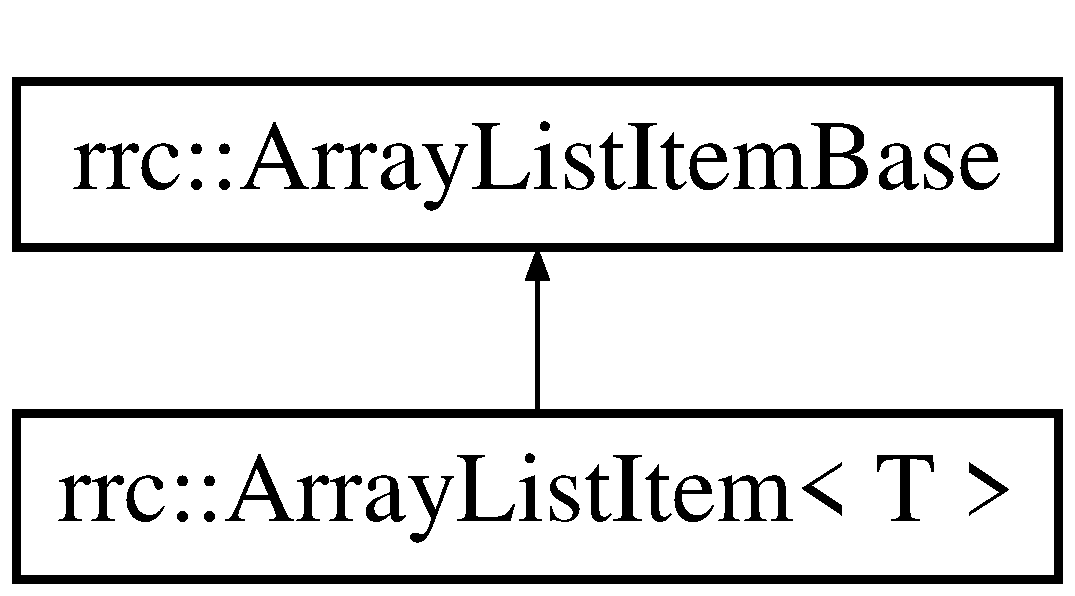
\includegraphics[height=2.000000cm]{classrrc_1_1_array_list_item}
\end{center}
\end{figure}
\subsection*{Public Member Functions}
\begin{DoxyCompactItemize}
\item 
\hypertarget{classrrc_1_1_array_list_item_ae67fbd0a39f63f753b63b5bbc9fe18c3}{}{\bfseries Array\+List\+Item} (const T \&val)\label{classrrc_1_1_array_list_item_ae67fbd0a39f63f753b63b5bbc9fe18c3}

\item 
\hypertarget{classrrc_1_1_array_list_item_a200a3d632bab9d5b2672377a4bce309f}{}{\bfseries operator T} ()\label{classrrc_1_1_array_list_item_a200a3d632bab9d5b2672377a4bce309f}

\item 
\hypertarget{classrrc_1_1_array_list_item_a729386debf17cdacf94146911c37f3e1}{}virtual const char {\bfseries operator\mbox{[}$\,$\mbox{]}} (const int \&pos) const \label{classrrc_1_1_array_list_item_a729386debf17cdacf94146911c37f3e1}

\item 
\hypertarget{classrrc_1_1_array_list_item_a0dfee6760c7c7e1a320dd2612491a908}{}\hyperlink{classrrc_1_1_array_list_item}{Array\+List\+Item}$<$ T $>$ \& {\bfseries operator=} (const \hyperlink{classrrc_1_1_array_list_item}{Array\+List\+Item}$<$ T $>$ \&rhs)\label{classrrc_1_1_array_list_item_a0dfee6760c7c7e1a320dd2612491a908}

\end{DoxyCompactItemize}


The documentation for this class was generated from the following file\+:\begin{DoxyCompactItemize}
\item 
rr\+Array\+List\+Item.\+h\end{DoxyCompactItemize}

\hypertarget{classrrc_1_1_array_list_item_base}{\section{Array\+List\+Item\+Base Class Reference}
\label{classrrc_1_1_array_list_item_base}\index{Array\+List\+Item\+Base@{Array\+List\+Item\+Base}}
}


Inherited by \hyperlink{classrrc_1_1_array_list_item}{Array\+List\+Item$<$ T $>$}.



The documentation for this class was generated from the following files\+:\begin{DoxyCompactItemize}
\item 
rr\+Array\+List\+Item\+Base.\+h\item 
rr\+Array\+List\+Item\+Base.\+cpp\end{DoxyCompactItemize}

\hypertarget{struct_r_r_c_data}{}\section{R\+R\+C\+Data Struct Reference}
\label{struct_r_r_c_data}\index{R\+R\+C\+Data@{R\+R\+C\+Data}}


Structure for the result type from the simulate calls. The client is responsible for freeing the R\+R\+C\+Data\+Ptr.  




{\ttfamily \#include $<$rrc\+\_\+types.\+h$>$}

\subsection*{Public Attributes}
\begin{DoxyCompactItemize}
\item 
int \hyperlink{struct_r_r_c_data_aaebd12e68638f3572eea166c7dd0af69}{R\+Size}
\item 
int \hyperlink{struct_r_r_c_data_a573616e93e0241d11b40ea56c708041b}{C\+Size}
\item 
double $\ast$ \hyperlink{struct_r_r_c_data_a4f2db98f036a01dca7168fee658bac0c}{Data}
\item 
double $\ast$ \hyperlink{struct_r_r_c_data_a2579ee2008f91694842f2278630852bf}{Weights}
\item 
char $\ast$$\ast$ \hyperlink{struct_r_r_c_data_a54acd2748775883500033984275be173}{Column\+Headers}
\end{DoxyCompactItemize}


\subsection{Detailed Description}
Structure for the result type from the simulate calls. The client is responsible for freeing the R\+R\+C\+Data\+Ptr. 

\subsection{Member Data Documentation}
\hypertarget{struct_r_r_c_data_a54acd2748775883500033984275be173}{}\index{R\+R\+C\+Data@{R\+R\+C\+Data}!Column\+Headers@{Column\+Headers}}
\index{Column\+Headers@{Column\+Headers}!R\+R\+C\+Data@{R\+R\+C\+Data}}
\subsubsection[{Column\+Headers}]{\setlength{\rightskip}{0pt plus 5cm}char$\ast$$\ast$ R\+R\+C\+Data\+::\+Column\+Headers}\label{struct_r_r_c_data_a54acd2748775883500033984275be173}
Pointer to an array of column header strings \hypertarget{struct_r_r_c_data_a573616e93e0241d11b40ea56c708041b}{}\index{R\+R\+C\+Data@{R\+R\+C\+Data}!C\+Size@{C\+Size}}
\index{C\+Size@{C\+Size}!R\+R\+C\+Data@{R\+R\+C\+Data}}
\subsubsection[{C\+Size}]{\setlength{\rightskip}{0pt plus 5cm}int R\+R\+C\+Data\+::\+C\+Size}\label{struct_r_r_c_data_a573616e93e0241d11b40ea56c708041b}
The number of columns in the data matrix \hypertarget{struct_r_r_c_data_a4f2db98f036a01dca7168fee658bac0c}{}\index{R\+R\+C\+Data@{R\+R\+C\+Data}!Data@{Data}}
\index{Data@{Data}!R\+R\+C\+Data@{R\+R\+C\+Data}}
\subsubsection[{Data}]{\setlength{\rightskip}{0pt plus 5cm}double$\ast$ R\+R\+C\+Data\+::\+Data}\label{struct_r_r_c_data_a4f2db98f036a01dca7168fee658bac0c}
A pointer to the data stored in the matrix. Access an element using Data\mbox{[}row$\ast$\+C\+Size + col\mbox{]} \hypertarget{struct_r_r_c_data_aaebd12e68638f3572eea166c7dd0af69}{}\index{R\+R\+C\+Data@{R\+R\+C\+Data}!R\+Size@{R\+Size}}
\index{R\+Size@{R\+Size}!R\+R\+C\+Data@{R\+R\+C\+Data}}
\subsubsection[{R\+Size}]{\setlength{\rightskip}{0pt plus 5cm}int R\+R\+C\+Data\+::\+R\+Size}\label{struct_r_r_c_data_aaebd12e68638f3572eea166c7dd0af69}
The number of rows in the data matrix \hypertarget{struct_r_r_c_data_a2579ee2008f91694842f2278630852bf}{}\index{R\+R\+C\+Data@{R\+R\+C\+Data}!Weights@{Weights}}
\index{Weights@{Weights}!R\+R\+C\+Data@{R\+R\+C\+Data}}
\subsubsection[{Weights}]{\setlength{\rightskip}{0pt plus 5cm}double$\ast$ R\+R\+C\+Data\+::\+Weights}\label{struct_r_r_c_data_a2579ee2008f91694842f2278630852bf}
A pointer to weights stored in the Weights matrix. Access an element using Weights\mbox{[}row$\ast$\+C\+Size + col\mbox{]} 

The documentation for this struct was generated from the following file\+:\begin{DoxyCompactItemize}
\item 
\hyperlink{rrc__types_8h}{rrc\+\_\+types.\+h}\end{DoxyCompactItemize}

\hypertarget{struct_r_r_complex}{\section{R\+R\+Complex Struct Reference}
\label{struct_r_r_complex}\index{R\+R\+Complex@{R\+R\+Complex}}
}


Structure for a complex number.  




{\ttfamily \#include $<$rrc\+\_\+types.\+h$>$}

\subsection*{Data Fields}
\begin{DoxyCompactItemize}
\item 
double \hyperlink{struct_r_r_complex_a5a6fce2fc5cae153945fea2c45beeb4f}{re}
\item 
double \hyperlink{struct_r_r_complex_a9aace20780eedccdde9fe2352ee4fb05}{imag}
\end{DoxyCompactItemize}


\subsection{Detailed Description}
Structure for a complex number. 

\subsection{Field Documentation}
\hypertarget{struct_r_r_complex_a9aace20780eedccdde9fe2352ee4fb05}{\index{R\+R\+Complex@{R\+R\+Complex}!imag@{imag}}
\index{imag@{imag}!R\+R\+Complex@{R\+R\+Complex}}
\subsubsection[{imag}]{\setlength{\rightskip}{0pt plus 5cm}double imag}}\label{struct_r_r_complex_a9aace20780eedccdde9fe2352ee4fb05}
imag part of complex number \hypertarget{struct_r_r_complex_a5a6fce2fc5cae153945fea2c45beeb4f}{\index{R\+R\+Complex@{R\+R\+Complex}!re@{re}}
\index{re@{re}!R\+R\+Complex@{R\+R\+Complex}}
\subsubsection[{re}]{\setlength{\rightskip}{0pt plus 5cm}double re}}\label{struct_r_r_complex_a5a6fce2fc5cae153945fea2c45beeb4f}
Real part of complex number 

The documentation for this struct was generated from the following file\+:\begin{DoxyCompactItemize}
\item 
\hyperlink{rrc__types_8h}{rrc\+\_\+types.\+h}\end{DoxyCompactItemize}

\hypertarget{struct_r_r_complex_matrix}{\section{R\+R\+Complex\+Matrix Struct Reference}
\label{struct_r_r_complex_matrix}\index{R\+R\+Complex\+Matrix@{R\+R\+Complex\+Matrix}}
}


Structure for a simple complex Matrix type.  




{\ttfamily \#include $<$rrc\+\_\+types.\+h$>$}

\subsection*{Data Fields}
\begin{DoxyCompactItemize}
\item 
int \hyperlink{struct_r_r_complex_matrix_a4d8512c879223c0e0d1522dae38e7819}{R\+Size}
\item 
int \hyperlink{struct_r_r_complex_matrix_a17c9a5894aa9cb3789346dcaa9c370bb}{C\+Size}
\item 
\hyperlink{rrc__types_8h_ada2046d7326c56ae29d8510fbf6622ee}{R\+R\+Complex\+Ptr} \hyperlink{struct_r_r_complex_matrix_a2853286fc6b37960bba4c8871da839fa}{Data}
\end{DoxyCompactItemize}


\subsection{Detailed Description}
Structure for a simple complex Matrix type. 

\subsection{Field Documentation}
\hypertarget{struct_r_r_complex_matrix_a17c9a5894aa9cb3789346dcaa9c370bb}{\index{R\+R\+Complex\+Matrix@{R\+R\+Complex\+Matrix}!C\+Size@{C\+Size}}
\index{C\+Size@{C\+Size}!R\+R\+Complex\+Matrix@{R\+R\+Complex\+Matrix}}
\subsubsection[{C\+Size}]{\setlength{\rightskip}{0pt plus 5cm}int C\+Size}}\label{struct_r_r_complex_matrix_a17c9a5894aa9cb3789346dcaa9c370bb}
The number of columns in the matrix \hypertarget{struct_r_r_complex_matrix_a2853286fc6b37960bba4c8871da839fa}{\index{R\+R\+Complex\+Matrix@{R\+R\+Complex\+Matrix}!Data@{Data}}
\index{Data@{Data}!R\+R\+Complex\+Matrix@{R\+R\+Complex\+Matrix}}
\subsubsection[{Data}]{\setlength{\rightskip}{0pt plus 5cm}{\bf R\+R\+Complex\+Ptr} Data}}\label{struct_r_r_complex_matrix_a2853286fc6b37960bba4c8871da839fa}
Items in the matrix stored as a linear array. Access an element using Data\mbox{[}row$\ast$\+C\+Size + col\mbox{]}, where i,j represent the row and column numberof the element. Indexing is from zero \hypertarget{struct_r_r_complex_matrix_a4d8512c879223c0e0d1522dae38e7819}{\index{R\+R\+Complex\+Matrix@{R\+R\+Complex\+Matrix}!R\+Size@{R\+Size}}
\index{R\+Size@{R\+Size}!R\+R\+Complex\+Matrix@{R\+R\+Complex\+Matrix}}
\subsubsection[{R\+Size}]{\setlength{\rightskip}{0pt plus 5cm}int R\+Size}}\label{struct_r_r_complex_matrix_a4d8512c879223c0e0d1522dae38e7819}
The number of rows in the matrix 

The documentation for this struct was generated from the following file\+:\begin{DoxyCompactItemize}
\item 
\hyperlink{rrc__types_8h}{rrc\+\_\+types.\+h}\end{DoxyCompactItemize}

\hypertarget{struct_r_r_complex_vector}{}\section{R\+R\+Complex\+Vector Struct Reference}
\label{struct_r_r_complex_vector}\index{R\+R\+Complex\+Vector@{R\+R\+Complex\+Vector}}


Structure for a simple complex Vector type.  




{\ttfamily \#include $<$rrc\+\_\+types.\+h$>$}

\subsection*{Public Attributes}
\begin{DoxyCompactItemize}
\item 
int \hyperlink{struct_r_r_complex_vector_a930d0decc2af8858b710280850d14d97}{Count}
\item 
\hyperlink{rrc__types_8h_ada2046d7326c56ae29d8510fbf6622ee}{R\+R\+Complex\+Ptr} \hyperlink{struct_r_r_complex_vector_ab09f6755f3856b4d97e0d40a7a7c2a20}{Data}
\end{DoxyCompactItemize}


\subsection{Detailed Description}
Structure for a simple complex Vector type. 

\subsection{Member Data Documentation}
\hypertarget{struct_r_r_complex_vector_a930d0decc2af8858b710280850d14d97}{}\index{R\+R\+Complex\+Vector@{R\+R\+Complex\+Vector}!Count@{Count}}
\index{Count@{Count}!R\+R\+Complex\+Vector@{R\+R\+Complex\+Vector}}
\subsubsection[{Count}]{\setlength{\rightskip}{0pt plus 5cm}int R\+R\+Complex\+Vector\+::\+Count}\label{struct_r_r_complex_vector_a930d0decc2af8858b710280850d14d97}
The number of elements in the vector \hypertarget{struct_r_r_complex_vector_ab09f6755f3856b4d97e0d40a7a7c2a20}{}\index{R\+R\+Complex\+Vector@{R\+R\+Complex\+Vector}!Data@{Data}}
\index{Data@{Data}!R\+R\+Complex\+Vector@{R\+R\+Complex\+Vector}}
\subsubsection[{Data}]{\setlength{\rightskip}{0pt plus 5cm}{\bf R\+R\+Complex\+Ptr} R\+R\+Complex\+Vector\+::\+Data}\label{struct_r_r_complex_vector_ab09f6755f3856b4d97e0d40a7a7c2a20}
Access an element using Data\mbox{[}i\mbox{]}, where i represents the index of the element. Indexing is from zero 

The documentation for this struct was generated from the following file\+:\begin{DoxyCompactItemize}
\item 
\hyperlink{rrc__types_8h}{rrc\+\_\+types.\+h}\end{DoxyCompactItemize}

\hypertarget{struct_r_r_double_matrix}{}\section{R\+R\+Double\+Matrix Struct Reference}
\label{struct_r_r_double_matrix}\index{R\+R\+Double\+Matrix@{R\+R\+Double\+Matrix}}


Structure for a simple double Matrix type.  




{\ttfamily \#include $<$rrc\+\_\+types.\+h$>$}

\subsection*{Public Attributes}
\begin{DoxyCompactItemize}
\item 
int \hyperlink{struct_r_r_double_matrix_a674431f97c6ce4a6ef05248a67ea1c54}{R\+Size}
\item 
int \hyperlink{struct_r_r_double_matrix_a0df8ed25504d41748cdde8c3e92062bb}{C\+Size}
\item 
double $\ast$ \hyperlink{struct_r_r_double_matrix_afeaa302597fc935e45634c8bd9e1e4b1}{Data}
\end{DoxyCompactItemize}


\subsection{Detailed Description}
Structure for a simple double Matrix type. 

\subsection{Member Data Documentation}
\hypertarget{struct_r_r_double_matrix_a0df8ed25504d41748cdde8c3e92062bb}{}\index{R\+R\+Double\+Matrix@{R\+R\+Double\+Matrix}!C\+Size@{C\+Size}}
\index{C\+Size@{C\+Size}!R\+R\+Double\+Matrix@{R\+R\+Double\+Matrix}}
\subsubsection[{C\+Size}]{\setlength{\rightskip}{0pt plus 5cm}int R\+R\+Double\+Matrix\+::\+C\+Size}\label{struct_r_r_double_matrix_a0df8ed25504d41748cdde8c3e92062bb}
The number of columns in the matrix \hypertarget{struct_r_r_double_matrix_afeaa302597fc935e45634c8bd9e1e4b1}{}\index{R\+R\+Double\+Matrix@{R\+R\+Double\+Matrix}!Data@{Data}}
\index{Data@{Data}!R\+R\+Double\+Matrix@{R\+R\+Double\+Matrix}}
\subsubsection[{Data}]{\setlength{\rightskip}{0pt plus 5cm}double$\ast$ R\+R\+Double\+Matrix\+::\+Data}\label{struct_r_r_double_matrix_afeaa302597fc935e45634c8bd9e1e4b1}
Items in the matrix stored as a linear array. Access an element using Data\mbox{[}row$\ast$\+C\+Size + col\mbox{]}, where i,j represent the row and column numberof the element. Indexing is from zero \hypertarget{struct_r_r_double_matrix_a674431f97c6ce4a6ef05248a67ea1c54}{}\index{R\+R\+Double\+Matrix@{R\+R\+Double\+Matrix}!R\+Size@{R\+Size}}
\index{R\+Size@{R\+Size}!R\+R\+Double\+Matrix@{R\+R\+Double\+Matrix}}
\subsubsection[{R\+Size}]{\setlength{\rightskip}{0pt plus 5cm}int R\+R\+Double\+Matrix\+::\+R\+Size}\label{struct_r_r_double_matrix_a674431f97c6ce4a6ef05248a67ea1c54}
The number of rows in the matrix 

The documentation for this struct was generated from the following file\+:\begin{DoxyCompactItemize}
\item 
\hyperlink{rrc__types_8h}{rrc\+\_\+types.\+h}\end{DoxyCompactItemize}

\hypertarget{struct_r_r_list}{}\section{R\+R\+List Struct Reference}
\label{struct_r_r_list}\index{R\+R\+List@{R\+R\+List}}


A list type, stores int, double, strings and lists.  




{\ttfamily \#include $<$rrc\+\_\+types.\+h$>$}

\subsection*{Public Attributes}
\begin{DoxyCompactItemize}
\item 
int \hyperlink{struct_r_r_list_a7026370b1982636d3dbba185f94eab12}{Count}
\item 
\hyperlink{rrc__types_8h_a79938364b69256c42480bb3a29ebf73e}{R\+R\+List\+Item\+Ptr} $\ast$ \hyperlink{struct_r_r_list_a3ab34807b735e2b319a6b4c5a09854dd}{Items}
\end{DoxyCompactItemize}


\subsection{Detailed Description}
A list type, stores int, double, strings and lists. 

\subsection{Member Data Documentation}
\hypertarget{struct_r_r_list_a7026370b1982636d3dbba185f94eab12}{}\index{R\+R\+List@{R\+R\+List}!Count@{Count}}
\index{Count@{Count}!R\+R\+List@{R\+R\+List}}
\subsubsection[{Count}]{\setlength{\rightskip}{0pt plus 5cm}int R\+R\+List\+::\+Count}\label{struct_r_r_list_a7026370b1982636d3dbba185f94eab12}
The number elements in this list \hypertarget{struct_r_r_list_a3ab34807b735e2b319a6b4c5a09854dd}{}\index{R\+R\+List@{R\+R\+List}!Items@{Items}}
\index{Items@{Items}!R\+R\+List@{R\+R\+List}}
\subsubsection[{Items}]{\setlength{\rightskip}{0pt plus 5cm}{\bf R\+R\+List\+Item\+Ptr}$\ast$ R\+R\+List\+::\+Items}\label{struct_r_r_list_a3ab34807b735e2b319a6b4c5a09854dd}
A pointer to a list of items 

The documentation for this struct was generated from the following file\+:\begin{DoxyCompactItemize}
\item 
\hyperlink{rrc__types_8h}{rrc\+\_\+types.\+h}\end{DoxyCompactItemize}

\hypertarget{struct_r_r_list_item}{}\section{R\+R\+List\+Item Struct Reference}
\label{struct_r_r_list_item}\index{R\+R\+List\+Item@{R\+R\+List\+Item}}


A single list element type.  




{\ttfamily \#include $<$rrc\+\_\+types.\+h$>$}

\subsection*{Public Attributes}
\begin{DoxyCompactItemize}
\item 
enum \hyperlink{rrc__types_8h_ab99437ab2e88aa90b7ebb8add042b25e}{List\+Item\+Type} \hyperlink{struct_r_r_list_item_a588ebb27c785286b9c809720be675a1d}{Item\+Type}
\item 
\begin{tabbing}
xx\=xx\=xx\=xx\=xx\=xx\=xx\=xx\=xx\=\kill
union \{\\
\>int \hyperlink{struct_r_r_list_item_ae15de7b1f1a6471da72b9772c53cc1da}{iValue}\\
\>double \hyperlink{struct_r_r_list_item_a6d5c2beab9812853769f9a32768207c2}{dValue}\\
\>char $\ast$ \hyperlink{struct_r_r_list_item_acfcabe3d9036821e5631222561c69951}{sValue}\\
\>struct \hyperlink{struct_r_r_list}{RRList} $\ast$ \hyperlink{struct_r_r_list_item_a7ba0216f30cfc65a905470abcf01534d}{lValue}\\
\} \hyperlink{struct_r_r_list_item_ade12f730888a69192a77e668a20fc00e}{data}\\

\end{tabbing}\end{DoxyCompactItemize}


\subsection{Detailed Description}
A single list element type. 

\subsection{Member Data Documentation}
\hypertarget{struct_r_r_list_item_ade12f730888a69192a77e668a20fc00e}{}\index{R\+R\+List\+Item@{R\+R\+List\+Item}!data@{data}}
\index{data@{data}!R\+R\+List\+Item@{R\+R\+List\+Item}}
\subsubsection[{data}]{\setlength{\rightskip}{0pt plus 5cm}union \{ ... \}   R\+R\+List\+Item\+::data}\label{struct_r_r_list_item_ade12f730888a69192a77e668a20fc00e}
Union \hypertarget{struct_r_r_list_item_a6d5c2beab9812853769f9a32768207c2}{}\index{R\+R\+List\+Item@{R\+R\+List\+Item}!d\+Value@{d\+Value}}
\index{d\+Value@{d\+Value}!R\+R\+List\+Item@{R\+R\+List\+Item}}
\subsubsection[{d\+Value}]{\setlength{\rightskip}{0pt plus 5cm}double R\+R\+List\+Item\+::d\+Value}\label{struct_r_r_list_item_a6d5c2beab9812853769f9a32768207c2}
Double value \hypertarget{struct_r_r_list_item_a588ebb27c785286b9c809720be675a1d}{}\index{R\+R\+List\+Item@{R\+R\+List\+Item}!Item\+Type@{Item\+Type}}
\index{Item\+Type@{Item\+Type}!R\+R\+List\+Item@{R\+R\+List\+Item}}
\subsubsection[{Item\+Type}]{\setlength{\rightskip}{0pt plus 5cm}enum {\bf List\+Item\+Type} R\+R\+List\+Item\+::\+Item\+Type}\label{struct_r_r_list_item_a588ebb27c785286b9c809720be675a1d}
The type of the item in this list element \hypertarget{struct_r_r_list_item_ae15de7b1f1a6471da72b9772c53cc1da}{}\index{R\+R\+List\+Item@{R\+R\+List\+Item}!i\+Value@{i\+Value}}
\index{i\+Value@{i\+Value}!R\+R\+List\+Item@{R\+R\+List\+Item}}
\subsubsection[{i\+Value}]{\setlength{\rightskip}{0pt plus 5cm}int R\+R\+List\+Item\+::i\+Value}\label{struct_r_r_list_item_ae15de7b1f1a6471da72b9772c53cc1da}
Integer value \hypertarget{struct_r_r_list_item_a7ba0216f30cfc65a905470abcf01534d}{}\index{R\+R\+List\+Item@{R\+R\+List\+Item}!l\+Value@{l\+Value}}
\index{l\+Value@{l\+Value}!R\+R\+List\+Item@{R\+R\+List\+Item}}
\subsubsection[{l\+Value}]{\setlength{\rightskip}{0pt plus 5cm}struct {\bf R\+R\+List}$\ast$ R\+R\+List\+Item\+::l\+Value}\label{struct_r_r_list_item_a7ba0216f30cfc65a905470abcf01534d}
List value \hypertarget{struct_r_r_list_item_acfcabe3d9036821e5631222561c69951}{}\index{R\+R\+List\+Item@{R\+R\+List\+Item}!s\+Value@{s\+Value}}
\index{s\+Value@{s\+Value}!R\+R\+List\+Item@{R\+R\+List\+Item}}
\subsubsection[{s\+Value}]{\setlength{\rightskip}{0pt plus 5cm}char$\ast$ R\+R\+List\+Item\+::s\+Value}\label{struct_r_r_list_item_acfcabe3d9036821e5631222561c69951}
String value 

The documentation for this struct was generated from the following file\+:\begin{DoxyCompactItemize}
\item 
\hyperlink{rrc__types_8h}{rrc\+\_\+types.\+h}\end{DoxyCompactItemize}

\hypertarget{struct_r_r_string_array}{}\section{R\+R\+String\+Array Struct Reference}
\label{struct_r_r_string_array}\index{R\+R\+String\+Array@{R\+R\+String\+Array}}


Structure for a simple vector of strings.  




{\ttfamily \#include $<$rrc\+\_\+types.\+h$>$}

\subsection*{Public Attributes}
\begin{DoxyCompactItemize}
\item 
int \hyperlink{struct_r_r_string_array_ac36cf70dc7a2832c24c5dec622fec2fb}{Count}
\item 
char $\ast$$\ast$ \hyperlink{struct_r_r_string_array_a848b81ad8aeeb26b39411c462aab1312}{String}
\end{DoxyCompactItemize}


\subsection{Detailed Description}
Structure for a simple vector of strings. 

\subsection{Member Data Documentation}
\hypertarget{struct_r_r_string_array_ac36cf70dc7a2832c24c5dec622fec2fb}{}\index{R\+R\+String\+Array@{R\+R\+String\+Array}!Count@{Count}}
\index{Count@{Count}!R\+R\+String\+Array@{R\+R\+String\+Array}}
\subsubsection[{Count}]{\setlength{\rightskip}{0pt plus 5cm}int R\+R\+String\+Array\+::\+Count}\label{struct_r_r_string_array_ac36cf70dc7a2832c24c5dec622fec2fb}
The number of elements in the string array \hypertarget{struct_r_r_string_array_a848b81ad8aeeb26b39411c462aab1312}{}\index{R\+R\+String\+Array@{R\+R\+String\+Array}!String@{String}}
\index{String@{String}!R\+R\+String\+Array@{R\+R\+String\+Array}}
\subsubsection[{String}]{\setlength{\rightskip}{0pt plus 5cm}char$\ast$$\ast$ R\+R\+String\+Array\+::\+String}\label{struct_r_r_string_array_a848b81ad8aeeb26b39411c462aab1312}
Points to an array of string items 

The documentation for this struct was generated from the following file\+:\begin{DoxyCompactItemize}
\item 
\hyperlink{rrc__types_8h}{rrc\+\_\+types.\+h}\end{DoxyCompactItemize}

\hypertarget{struct_r_r_vector}{\section{R\+R\+Vector Struct Reference}
\label{struct_r_r_vector}\index{R\+R\+Vector@{R\+R\+Vector}}
}


Structure for a simple vector of doubles.  




{\ttfamily \#include $<$rrc\+\_\+types.\+h$>$}

\subsection*{Data Fields}
\begin{DoxyCompactItemize}
\item 
int \hyperlink{struct_r_r_vector_aad462966ed963f892117056de1eba502}{Count}
\item 
double $\ast$ \hyperlink{struct_r_r_vector_a7c5cbda3aa940f4b0d6e8a1679307dfc}{Data}
\end{DoxyCompactItemize}


\subsection{Detailed Description}
Structure for a simple vector of doubles. 

\subsection{Field Documentation}
\hypertarget{struct_r_r_vector_aad462966ed963f892117056de1eba502}{\index{R\+R\+Vector@{R\+R\+Vector}!Count@{Count}}
\index{Count@{Count}!R\+R\+Vector@{R\+R\+Vector}}
\subsubsection[{Count}]{\setlength{\rightskip}{0pt plus 5cm}int Count}}\label{struct_r_r_vector_aad462966ed963f892117056de1eba502}
The number of elements in the vector \hypertarget{struct_r_r_vector_a7c5cbda3aa940f4b0d6e8a1679307dfc}{\index{R\+R\+Vector@{R\+R\+Vector}!Data@{Data}}
\index{Data@{Data}!R\+R\+Vector@{R\+R\+Vector}}
\subsubsection[{Data}]{\setlength{\rightskip}{0pt plus 5cm}double$\ast$ Data}}\label{struct_r_r_vector_a7c5cbda3aa940f4b0d6e8a1679307dfc}
Points to an array of double items 

The documentation for this struct was generated from the following file\+:\begin{DoxyCompactItemize}
\item 
\hyperlink{rrc__types_8h}{rrc\+\_\+types.\+h}\end{DoxyCompactItemize}

\hypertarget{classrrc_1_1_string_list}{\section{String\+List Class Reference}
\label{classrrc_1_1_string_list}\index{String\+List@{String\+List}}
}
\subsection*{Public Member Functions}
\begin{DoxyCompactItemize}
\item 
\hypertarget{classrrc_1_1_string_list_ae1e0bca30bc21edd66e7dd2b539273f4}{{\bfseries String\+List} (char $\ast$$\ast$string\+List, const int \&count)}\label{classrrc_1_1_string_list_ae1e0bca30bc21edd66e7dd2b539273f4}

\item 
\hypertarget{classrrc_1_1_string_list_a6306d63c1e79ab13cb62c1937722a06f}{{\bfseries String\+List} (const string \&str, const string \&delimiters=\char`\"{}, \char`\"{})}\label{classrrc_1_1_string_list_a6306d63c1e79ab13cb62c1937722a06f}

\item 
\hypertarget{classrrc_1_1_string_list_aec20e4743e6cebb9a3c14f04eee6ea5b}{{\bfseries String\+List} (const vector$<$ string $>$ \&strings)}\label{classrrc_1_1_string_list_aec20e4743e6cebb9a3c14f04eee6ea5b}

\item 
\hypertarget{classrrc_1_1_string_list_a2c6607735f8c410ce3ab82c1b88fc6f7}{{\bfseries String\+List} (const \hyperlink{classrrc_1_1_string_list}{String\+List} \&cp)}\label{classrrc_1_1_string_list_a2c6607735f8c410ce3ab82c1b88fc6f7}

\item 
\hypertarget{classrrc_1_1_string_list_a6dcfcea51506e87c9bbb2cf3f65751f7}{{\bfseries String\+List} (\hyperlink{rrc__types_8h_a7c9475df6c7337d99482b13a365e7596}{rrc\+::\+R\+R\+String\+Array\+Ptr} cp)}\label{classrrc_1_1_string_list_a6dcfcea51506e87c9bbb2cf3f65751f7}

\item 
\hypertarget{classrrc_1_1_string_list_ac3831ed58535977c2188dff41fbd2bcd}{void {\bfseries Insert\+At} (const int \&index, const string \&item)}\label{classrrc_1_1_string_list_ac3831ed58535977c2188dff41fbd2bcd}

\item 
\hypertarget{classrrc_1_1_string_list_aff1a1c047f187d1c50ef09f7c803d9f9}{void {\bfseries Append} (const \hyperlink{classrrc_1_1_string_list}{String\+List} \&list)}\label{classrrc_1_1_string_list_aff1a1c047f187d1c50ef09f7c803d9f9}

\item 
\hypertarget{classrrc_1_1_string_list_aba253d1961eaa72ab2ef2bd9610ec961}{string {\bfseries As\+String} (const string \&delimiter=\char`\"{},\char`\"{}) const }\label{classrrc_1_1_string_list_aba253d1961eaa72ab2ef2bd9610ec961}

\item 
unsigned int \hyperlink{classrrc_1_1_string_list_a90ca964ebcc1b02bbcde225edd49e812}{size} () const 
\item 
\hypertarget{classrrc_1_1_string_list_a074f9905a87bb9395d21d9f4bc8c459f}{unsigned int {\bfseries Count} () const }\label{classrrc_1_1_string_list_a074f9905a87bb9395d21d9f4bc8c459f}

\item 
\hypertarget{classrrc_1_1_string_list_a2d4108b1b2a5fdc64f823cb0cfb1a35d}{\hyperlink{classrrc_1_1_string_list}{String\+List} \& {\bfseries operator=} (const \hyperlink{classrrc_1_1_string_list}{String\+List} \&rhs)}\label{classrrc_1_1_string_list_a2d4108b1b2a5fdc64f823cb0cfb1a35d}

\item 
\hypertarget{classrrc_1_1_string_list_ac476e20b26f934e94e4c2d19ae41910b}{\hyperlink{classrrc_1_1_string_list}{String\+List} \& {\bfseries operator=} (const vector$<$ string $>$ \&rhs)}\label{classrrc_1_1_string_list_ac476e20b26f934e94e4c2d19ae41910b}

\item 
\hypertarget{classrrc_1_1_string_list_a6e0b8928b22a4a30d3fb04bc851fc994}{string \& {\bfseries operator\mbox{[}$\,$\mbox{]}} (const int \&index)}\label{classrrc_1_1_string_list_a6e0b8928b22a4a30d3fb04bc851fc994}

\item 
\hypertarget{classrrc_1_1_string_list_a11634ec13410f134b8e96302a9c19b31}{const string \& {\bfseries operator\mbox{[}$\,$\mbox{]}} (const int \&index) const }\label{classrrc_1_1_string_list_a11634ec13410f134b8e96302a9c19b31}

\item 
\hypertarget{classrrc_1_1_string_list_a3d27c5a58e8cd6708d62f485ff4256ef}{\hyperlink{classrrc_1_1_string_list}{String\+List} {\bfseries operator-\/} (const \hyperlink{classrrc_1_1_string_list}{String\+List} \&rhs)}\label{classrrc_1_1_string_list_a3d27c5a58e8cd6708d62f485ff4256ef}

\item 
\hypertarget{classrrc_1_1_string_list_a760a68ea559d91b53fd2a24285d20a57}{void {\bfseries remove\+At} (const int \&index)}\label{classrrc_1_1_string_list_a760a68ea559d91b53fd2a24285d20a57}

\item 
\hypertarget{classrrc_1_1_string_list_a896cb3514a30b3952977bfecad378f5e}{int {\bfseries find} (const string \&item)}\label{classrrc_1_1_string_list_a896cb3514a30b3952977bfecad378f5e}

\item 
\hypertarget{classrrc_1_1_string_list_a8f24a28ce964c32be53db5fd15e284f5}{int {\bfseries index\+Of} (const string \&item)}\label{classrrc_1_1_string_list_a8f24a28ce964c32be53db5fd15e284f5}

\item 
\hypertarget{classrrc_1_1_string_list_ac8bb3912a3ce86b15842e79d0b421204}{void {\bfseries clear} ()}\label{classrrc_1_1_string_list_ac8bb3912a3ce86b15842e79d0b421204}

\item 
\hypertarget{classrrc_1_1_string_list_a9a4d7b0a805f99ab95362516ee336b3e}{void {\bfseries empty} ()}\label{classrrc_1_1_string_list_a9a4d7b0a805f99ab95362516ee336b3e}

\item 
\hypertarget{classrrc_1_1_string_list_aca34f34ee9b97830dccc8a4d7f96e551}{bool {\bfseries Contains} (const string \&item) const }\label{classrrc_1_1_string_list_aca34f34ee9b97830dccc8a4d7f96e551}

\item 
\hypertarget{classrrc_1_1_string_list_aa97fd3fa0e7997321f117c96be4e68cd}{bool {\bfseries Dont\+Contain} (const string \&item) const }\label{classrrc_1_1_string_list_aa97fd3fa0e7997321f117c96be4e68cd}

\item 
\hypertarget{classrrc_1_1_string_list_a564a583cd9dced158058e75d2250d64b}{void {\bfseries add} (const string \&item)}\label{classrrc_1_1_string_list_a564a583cd9dced158058e75d2250d64b}

\item 
\hypertarget{classrrc_1_1_string_list_ad64543071cdb2f63020c171deaef342c}{vector$<$ string $>$\+::iterator {\bfseries begin} ()}\label{classrrc_1_1_string_list_ad64543071cdb2f63020c171deaef342c}

\item 
\hypertarget{classrrc_1_1_string_list_a3ca73b915613e6ddd538bf01a06dfb4a}{vector$<$ string $>$\+::iterator {\bfseries end} ()}\label{classrrc_1_1_string_list_a3ca73b915613e6ddd538bf01a06dfb4a}

\item 
\hypertarget{classrrc_1_1_string_list_af5dd8b48496fae30a18d14459b803cfe}{void {\bfseries Pre\+Fix} (const string \&fix)}\label{classrrc_1_1_string_list_af5dd8b48496fae30a18d14459b803cfe}

\item 
\hypertarget{classrrc_1_1_string_list_afd0d188352312d299d954879a1fbd094}{void {\bfseries Post\+Fix} (const string \&fix)}\label{classrrc_1_1_string_list_afd0d188352312d299d954879a1fbd094}

\item 
\hyperlink{classrrc_1_1_string_list_a6b71378b966274510e49991bd1234c6b}{operator const vector$<$ string $>$ \&} () const 
\end{DoxyCompactItemize}
\subsection*{Protected Attributes}
\begin{DoxyCompactItemize}
\item 
\hypertarget{classrrc_1_1_string_list_a976a0752d85b65529ae592627f586f5a}{vector$<$ string $>$ {\bfseries m\+Strings}}\label{classrrc_1_1_string_list_a976a0752d85b65529ae592627f586f5a}

\item 
\hypertarget{classrrc_1_1_string_list_a5fb77339b8b0e2edabdd22785268494e}{vector$<$ string $>$\+::iterator {\bfseries m\+L\+I}}\label{classrrc_1_1_string_list_a5fb77339b8b0e2edabdd22785268494e}

\end{DoxyCompactItemize}
\subsection*{Friends}
\begin{DoxyCompactItemize}
\item 
\hypertarget{classrrc_1_1_string_list_aa3ce47607ddae8b81ab08d118918a5fc}{R\+R\+\_\+\+D\+E\+C\+L\+S\+P\+E\+C friend ostream \& {\bfseries operator$<$$<$} (ostream \&stream, const \hyperlink{classrrc_1_1_string_list}{String\+List} \&list)}\label{classrrc_1_1_string_list_aa3ce47607ddae8b81ab08d118918a5fc}

\end{DoxyCompactItemize}


\subsection{Member Function Documentation}
\hypertarget{classrrc_1_1_string_list_a6b71378b966274510e49991bd1234c6b}{\index{rrc\+::\+String\+List@{rrc\+::\+String\+List}!operator const vector$<$ string $>$ \&@{operator const vector$<$ string $>$ \&}}
\index{operator const vector$<$ string $>$ \&@{operator const vector$<$ string $>$ \&}!rrc\+::\+String\+List@{rrc\+::\+String\+List}}
\subsubsection[{operator const vector$<$ string $>$ \&}]{\setlength{\rightskip}{0pt plus 5cm}operator const vector$<$ string $>$ \& (
\begin{DoxyParamCaption}
{}
\end{DoxyParamCaption}
) const\hspace{0.3cm}{\ttfamily [inline]}}}\label{classrrc_1_1_string_list_a6b71378b966274510e49991bd1234c6b}
so we can start getting rid of this and using standard vector$<$string$>$ \hypertarget{classrrc_1_1_string_list_a90ca964ebcc1b02bbcde225edd49e812}{\index{rrc\+::\+String\+List@{rrc\+::\+String\+List}!size@{size}}
\index{size@{size}!rrc\+::\+String\+List@{rrc\+::\+String\+List}}
\subsubsection[{size}]{\setlength{\rightskip}{0pt plus 5cm}unsigned int size (
\begin{DoxyParamCaption}
{}
\end{DoxyParamCaption}
) const}}\label{classrrc_1_1_string_list_a90ca964ebcc1b02bbcde225edd49e812}
get the size to be compatible with vector$<$string$>$ 

The documentation for this class was generated from the following files\+:\begin{DoxyCompactItemize}
\item 
rrc\+String\+List.\+h\item 
rrc\+String\+List.\+cpp\end{DoxyCompactItemize}

\chapter{File Documentation}
\hypertarget{rrc__api_8cpp}{\section{rrc\+\_\+api.\+cpp File Reference}
\label{rrc__api_8cpp}\index{rrc\+\_\+api.\+cpp@{rrc\+\_\+api.\+cpp}}
}


road\+Runner C A\+P\+I 2012  


{\ttfamily \#include $<$string$>$}\\*
{\ttfamily \#include $<$iostream$>$}\\*
{\ttfamily \#include $<$sstream$>$}\\*
{\ttfamily \#include $<$fstream$>$}\\*
{\ttfamily \#include \char`\"{}rr\+Road\+Runner.\+h\char`\"{}}\\*
{\ttfamily \#include \char`\"{}rr\+Road\+Runner\+Options.\+h\char`\"{}}\\*
{\ttfamily \#include \char`\"{}rr\+Executable\+Model.\+h\char`\"{}}\\*
{\ttfamily \#include \char`\"{}rr\+Compiler.\+h\char`\"{}}\\*
{\ttfamily \#include \char`\"{}rr\+Logger.\+h\char`\"{}}\\*
{\ttfamily \#include \char`\"{}rr\+Exception.\+h\char`\"{}}\\*
{\ttfamily \#include \char`\"{}rr\+Version\+Info.\+h\char`\"{}}\\*
{\ttfamily \#include \char`\"{}rr\+Utils.\+h\char`\"{}}\\*
{\ttfamily \#include \char`\"{}rrc\+\_\+types.\+h\char`\"{}}\\*
{\ttfamily \#include \char`\"{}rrc\+\_\+api.\+h\char`\"{}}\\*
{\ttfamily \#include \char`\"{}rrc\+\_\+utilities.\+h\char`\"{}}\\*
{\ttfamily \#include \char`\"{}rrc\+\_\+cpp\+\_\+support.\+h\char`\"{}}\\*
{\ttfamily \#include \char`\"{}Integrator.\+h\char`\"{}}\\*
{\ttfamily \#include \char`\"{}Steady\+State\+Solver.\+h\char`\"{}}\\*
{\ttfamily \#include \char`\"{}Dictionary.\+h\char`\"{}}\\*
{\ttfamily \#include \char`\"{}rr\+Config.\+h\char`\"{}}\\*
{\ttfamily \#include $<$unistd.\+h$>$}\\*
{\ttfamily \#include $<$limits.\+h$>$}\\*
\subsection*{Macros}
\begin{DoxyCompactItemize}
\item 
\hypertarget{rrc__api_8cpp_af3b54520e40857c14ac49a364ba094a8}{\#define \hyperlink{rrc__api_8cpp_af3b54520e40857c14ac49a364ba094a8}{R\+R\+\_\+\+M\+A\+X\+\_\+\+P\+A\+T\+H}~P\+A\+T\+H\+\_\+\+M\+A\+X}\label{rrc__api_8cpp_af3b54520e40857c14ac49a364ba094a8}

\begin{DoxyCompactList}\small\item\em macro for M\+A\+X\+\_\+\+P\+A\+T\+H \end{DoxyCompactList}\end{DoxyCompactItemize}
\subsection*{Functions}
\begin{DoxyCompactItemize}
\item 
\hyperlink{rrc__types_8h_a1d68f0592372208fa5a5f2799ea4b3ae}{R\+R\+Handle} \hyperlink{group__initialization_gac5b4dbf9108edb1ea6e315379e5576e0}{create\+R\+R\+Instance} ()
\begin{DoxyCompactList}\small\item\em Initialize a new road\+Runner instance and return a handle to it. \end{DoxyCompactList}\item 
\hyperlink{rrc__types_8h_a1d68f0592372208fa5a5f2799ea4b3ae}{R\+R\+Handle} \hyperlink{group__initialization_ga03b0c84179407dda1f4ae19a66dacf47}{create\+R\+R\+Instance\+Ex} (const char $\ast$temp\+Folder, const char $\ast$compiler\+\_\+cstr)
\begin{DoxyCompactList}\small\item\em Initialize a new road\+Runner instance and return a handle to it. \end{DoxyCompactList}\item 
char $\ast$ \hyperlink{group__initialization_ga0717cdb4fb8684f97a2b6793544ba6e2}{get\+Install\+Folder} ()
\begin{DoxyCompactList}\small\item\em Returns the folder in which the Road\+Runner A\+P\+I is installed. \end{DoxyCompactList}\item 
bool \hyperlink{group__initialization_gad1eb8bfdac1addc406f8ea5ee6d32c8d}{set\+Install\+Folder} (const char $\ast$folder)
\begin{DoxyCompactList}\small\item\em Set the internal string containing the folder in where the Road\+Runner C A\+P\+I is installed. \end{DoxyCompactList}\item 
char $\ast$ \hyperlink{group__utility_ga0201bfe0112ad64005f753c3ef9f967a}{get\+A\+P\+I\+Version} ()
\begin{DoxyCompactList}\small\item\em Retrieve the current version number of the C A\+P\+I library. \end{DoxyCompactList}\item 
char $\ast$ \hyperlink{group__utility_ga691ff48bcf6063a8544ee17c78c08a2e}{get\+C\+P\+P\+A\+P\+I\+Version} (\hyperlink{rrc__types_8h_a1d68f0592372208fa5a5f2799ea4b3ae}{R\+R\+Handle} handle)
\begin{DoxyCompactList}\small\item\em Retrieve the current version number of the C++ A\+P\+I (Core Road\+Runner A\+P\+I) library. \end{DoxyCompactList}\item 
int {\bfseries get\+Version} ()
\item 
char $\ast$ {\bfseries get\+Version\+Str} ()
\item 
char $\ast$ {\bfseries get\+Version\+Ex} ()
\item 
char $\ast$ \hyperlink{group__utility_gad2d89e6329c3f10496e2eeb3af705541}{get\+R\+R\+C\+A\+P\+I\+Location} ()
\begin{DoxyCompactList}\small\item\em Retrieve the directory path of the shared rr\+C\+Api library. \end{DoxyCompactList}\item 
char $\ast$ \hyperlink{group__utility_gab6fdd755cfe37c9f3d6ba9afa2d26843}{get\+Copyright} ()
\begin{DoxyCompactList}\small\item\em Retrieve the current copyright notice for the library. \end{DoxyCompactList}\item 
char $\ast$ \hyperlink{group__utility_ga45c49fe2586cf9feacb66d1c3253bb64}{get\+Info} (\hyperlink{rrc__types_8h_a1d68f0592372208fa5a5f2799ea4b3ae}{R\+R\+Handle} handle)
\begin{DoxyCompactList}\small\item\em Retrieve info about current state of roadrunner, e.\+g. loaded model, conservation\+Analysis etc. \end{DoxyCompactList}\item 
char $\ast$ \hyperlink{group__utility_ga6375654feeeed364756d04996ffefca0}{get\+Extended\+A\+P\+I\+Info} ()
\begin{DoxyCompactList}\small\item\em Retrieve extended A\+P\+I info. \end{DoxyCompactList}\item 
char $\ast$ \hyperlink{group__utility_ga776c22cd6c98c3e37a3837d95ed9ebfc}{getlib\+S\+B\+M\+L\+Version} (\hyperlink{rrc__types_8h_a1d68f0592372208fa5a5f2799ea4b3ae}{R\+R\+Handle} handle)
\begin{DoxyCompactList}\small\item\em Retrieve the current version number of the lib\+S\+B\+M\+L library. \end{DoxyCompactList}\item 
char $\ast$ \hyperlink{group__loadsave_ga25a051f0d6f624e5f1634911cf545d79}{get\+Current\+S\+B\+M\+L} (\hyperlink{rrc__types_8h_a1d68f0592372208fa5a5f2799ea4b3ae}{R\+R\+Handle} handle)
\begin{DoxyCompactList}\small\item\em Retrieve the {\bfseries current state} of the model in the form of an S\+B\+M\+L string. \end{DoxyCompactList}\item 
bool \hyperlink{group__initialization_gaf336e356c4647feec53d5f8ca02614d5}{set\+Compute\+And\+Assign\+Conservation\+Laws} (\hyperlink{rrc__types_8h_a1d68f0592372208fa5a5f2799ea4b3ae}{R\+R\+Handle} handle, const bool On\+Or\+Off)
\begin{DoxyCompactList}\small\item\em Enable or disable conservation analysis. \end{DoxyCompactList}\item 
bool \hyperlink{group__utility_ga8d788961a18c347e246bbe6011ca4df8}{set\+Temp\+Folder} (\hyperlink{rrc__types_8h_a1d68f0592372208fa5a5f2799ea4b3ae}{R\+R\+Handle} handle, const char $\ast$folder)
\begin{DoxyCompactList}\small\item\em Set the path to the temporary folder where the C code will be stored. \end{DoxyCompactList}\item 
char $\ast$ \hyperlink{group__utility_gaab1f66913fef8d529635267744ac3de6}{get\+Temp\+Folder} (\hyperlink{rrc__types_8h_a1d68f0592372208fa5a5f2799ea4b3ae}{R\+R\+Handle} handle)
\begin{DoxyCompactList}\small\item\em Retrieve the current temporary folder path. \end{DoxyCompactList}\item 
bool \hyperlink{group__utility_ga359c597f4e2f825bbf054f76e2df46d9}{set\+Compiler} (\hyperlink{rrc__types_8h_a1d68f0592372208fa5a5f2799ea4b3ae}{R\+R\+Handle} handle, const char $\ast$f\+Name)
\begin{DoxyCompactList}\small\item\em Set the path and filename to the compiler to be used by roadrunner. \end{DoxyCompactList}\item 
\hypertarget{group__utility_gacce5637b3025d0f23a5baedd87538ba5}{char $\ast$ \hyperlink{group__utility_gacce5637b3025d0f23a5baedd87538ba5}{get\+Compiler} (\hyperlink{rrc__types_8h_a1d68f0592372208fa5a5f2799ea4b3ae}{R\+R\+Handle} handle)}\label{group__utility_gacce5637b3025d0f23a5baedd87538ba5}

\begin{DoxyCompactList}\small\item\em Get the name of the compiler currently being used by roadrunner. \end{DoxyCompactList}\item 
bool \hyperlink{group__utility_ga67ef111be16bc217142f7042c4c73650}{set\+Compiler\+Location} (\hyperlink{rrc__types_8h_a1d68f0592372208fa5a5f2799ea4b3ae}{R\+R\+Handle} handle, const char $\ast$folder)
\begin{DoxyCompactList}\small\item\em Set the path to a folder containing the compiler to be used. \end{DoxyCompactList}\item 
char $\ast$ \hyperlink{group__utility_gaa7c663617b26a30e2d6d6ec87f8e8a1a}{get\+Compiler\+Location} (\hyperlink{rrc__types_8h_a1d68f0592372208fa5a5f2799ea4b3ae}{R\+R\+Handle} handle)
\begin{DoxyCompactList}\small\item\em Get the path to a folder containing the compiler being used. \end{DoxyCompactList}\item 
bool \hyperlink{group__utility_gaf6bd5a3e646e8c16b678bd7367662507}{set\+Support\+Code\+Folder} (\hyperlink{rrc__types_8h_a1d68f0592372208fa5a5f2799ea4b3ae}{R\+R\+Handle} handle, const char $\ast$folder)
\begin{DoxyCompactList}\small\item\em Set the path to a folder containing support code for model generation. \end{DoxyCompactList}\item 
char $\ast$ \hyperlink{group__utility_ga9ea74c25e9f56b9e3176475510a7d304}{get\+Support\+Code\+Folder} (\hyperlink{rrc__types_8h_a1d68f0592372208fa5a5f2799ea4b3ae}{R\+R\+Handle} handle)
\begin{DoxyCompactList}\small\item\em Get the path to a folder containing support code. \end{DoxyCompactList}\item 
char $\ast$ \hyperlink{group__utility_ga8572aeabff24d30099b45901b8992120}{get\+Working\+Directory} ()
\begin{DoxyCompactList}\small\item\em Retrieve the current working directory path. \end{DoxyCompactList}\item 
bool \hyperlink{group__loadsave_ga275b8f8d7350505c383fdc9634713041}{load\+S\+B\+M\+L\+From\+File} (\hyperlink{rrc__types_8h_a1d68f0592372208fa5a5f2799ea4b3ae}{R\+R\+Handle} \+\_\+handle, const char $\ast$file\+Name)
\begin{DoxyCompactList}\small\item\em Load a model from a S\+B\+M\+L file. \end{DoxyCompactList}\item 
bool \hyperlink{group__loadsave_gaba8e934b2e2c045312686c5e857aacab}{load\+S\+B\+M\+L\+From\+File\+E} (\hyperlink{rrc__types_8h_a1d68f0592372208fa5a5f2799ea4b3ae}{R\+R\+Handle} \+\_\+handle, const char $\ast$file\+Name, bool force\+Recompile)
\begin{DoxyCompactList}\small\item\em Load a model from a S\+B\+M\+L file, force recompilation. \end{DoxyCompactList}\item 
bool \hyperlink{group__loadsave_gafb3515fd8472da389f5f24530017f037}{load\+S\+B\+M\+L} (\hyperlink{rrc__types_8h_a1d68f0592372208fa5a5f2799ea4b3ae}{R\+R\+Handle} handle, const char $\ast$sbml)
\begin{DoxyCompactList}\small\item\em Load a model from an S\+B\+M\+L string. \end{DoxyCompactList}\item 
bool \hyperlink{group__loadsave_ga80ede4ecc6e4e697e289d187c1a8d844}{load\+S\+B\+M\+L\+Ex} (\hyperlink{rrc__types_8h_a1d68f0592372208fa5a5f2799ea4b3ae}{R\+R\+Handle} handle, const char $\ast$sbml, bool force\+Recompile)
\begin{DoxyCompactList}\small\item\em Load a model from an S\+B\+M\+L string. \end{DoxyCompactList}\item 
bool \hyperlink{group__loadsave_ga93797731c7c87ca775b2d4ce1ed3178c}{load\+Simulation\+Settings} (\hyperlink{rrc__types_8h_a1d68f0592372208fa5a5f2799ea4b3ae}{R\+R\+Handle} handle, const char $\ast$file\+Name)
\begin{DoxyCompactList}\small\item\em Load simulation settings from a file. \end{DoxyCompactList}\item 
char $\ast$ \hyperlink{group__loadsave_ga1ad04f6a6ac4ffccd25a056490bb6f53}{get\+S\+B\+M\+L} (\hyperlink{rrc__types_8h_a1d68f0592372208fa5a5f2799ea4b3ae}{R\+R\+Handle} handle)
\begin{DoxyCompactList}\small\item\em Retrieve the S\+B\+M\+L model that was last loaded into road\+Runner. \end{DoxyCompactList}\item 
bool \hyperlink{group__loadsave_ga533342a784ba4e48c16cc59e2307f609}{is\+Model\+Loaded} (\hyperlink{rrc__types_8h_a1d68f0592372208fa5a5f2799ea4b3ae}{R\+R\+Handle} handle)
\begin{DoxyCompactList}\small\item\em check if a model is loaded \end{DoxyCompactList}\item 
bool \hyperlink{group__loadsave_ga78e637849c0d221eeee1168d101fcf30}{clear\+Model} (\hyperlink{rrc__types_8h_a1d68f0592372208fa5a5f2799ea4b3ae}{R\+R\+Handle} handle)
\begin{DoxyCompactList}\small\item\em Unload current model. \end{DoxyCompactList}\item 
bool \hyperlink{group__simulation_gaa5898253f7c907443f5df78387e3e77c}{set\+Time\+Start} (\hyperlink{rrc__types_8h_a1d68f0592372208fa5a5f2799ea4b3ae}{R\+R\+Handle} handle, const double time\+Start)
\begin{DoxyCompactList}\small\item\em Set the time start for a time course simulation. \end{DoxyCompactList}\item 
bool \hyperlink{group__simulation_gaf609c0853e0d053f43f4ef4f068f002f}{set\+Time\+End} (\hyperlink{rrc__types_8h_a1d68f0592372208fa5a5f2799ea4b3ae}{R\+R\+Handle} handle, const double time\+End)
\begin{DoxyCompactList}\small\item\em Set the time end for a time course simulation. \end{DoxyCompactList}\item 
bool \hyperlink{group__simulation_ga13f8b0ebfd2effe5264c3fed0ebb2471}{set\+Num\+Points} (\hyperlink{rrc__types_8h_a1d68f0592372208fa5a5f2799ea4b3ae}{R\+R\+Handle} handle, const int nr\+Points)
\begin{DoxyCompactList}\small\item\em Set the number of points to generate in a time course simulation. \end{DoxyCompactList}\item 
bool \hyperlink{group__simulation_gaf302d02e9f0d57dd05995a7a211e5236}{get\+Time\+Start} (\hyperlink{rrc__types_8h_a1d68f0592372208fa5a5f2799ea4b3ae}{R\+R\+Handle} handle, double $\ast$time\+Start)
\begin{DoxyCompactList}\small\item\em Get the value of the current time start. \end{DoxyCompactList}\item 
bool \hyperlink{group__simulation_ga1130df59dce620b619e3e58874025e57}{get\+Time\+End} (\hyperlink{rrc__types_8h_a1d68f0592372208fa5a5f2799ea4b3ae}{R\+R\+Handle} handle, double $\ast$time\+End)
\begin{DoxyCompactList}\small\item\em Get the value of the current time end. \end{DoxyCompactList}\item 
bool \hyperlink{group__simulation_ga3e14da4bd986a908e4f6bcfc42c20717}{get\+Num\+Points} (\hyperlink{rrc__types_8h_a1d68f0592372208fa5a5f2799ea4b3ae}{R\+R\+Handle} handle, int $\ast$num\+Points)
\begin{DoxyCompactList}\small\item\em Get the value of the current number of points. \end{DoxyCompactList}\item 
bool \hyperlink{group__simulation_gabc78e3202e85470f1c0e380a8988fc9e}{set\+Time\+Course\+Selection\+List} (\hyperlink{rrc__types_8h_a1d68f0592372208fa5a5f2799ea4b3ae}{R\+R\+Handle} handle, const char $\ast$list)
\begin{DoxyCompactList}\small\item\em Set the selection list for output from simulate(void) or simulate\+Ex(void) \end{DoxyCompactList}\item 
\hyperlink{rrc__types_8h_a7c9475df6c7337d99482b13a365e7596}{R\+R\+String\+Array\+Ptr} \hyperlink{group__simulation_ga4c2ce3bcc97cbd6a5dcae423dfeeba0c}{get\+Time\+Course\+Selection\+List} (\hyperlink{rrc__types_8h_a1d68f0592372208fa5a5f2799ea4b3ae}{R\+R\+Handle} handle)
\begin{DoxyCompactList}\small\item\em Get the current selection list for simulate(void) or simulate\+Ex(void) \end{DoxyCompactList}\item 
\hyperlink{rrc__types_8h_a9da8b124eb9c3c0045f8926c6a420b4a}{R\+R\+C\+Data\+Ptr} \hyperlink{group__simulation_ga55c9ef1913377542f61d1d622911cc7b}{simulate} (\hyperlink{rrc__types_8h_a1d68f0592372208fa5a5f2799ea4b3ae}{R\+R\+Handle} handle)
\begin{DoxyCompactList}\small\item\em Carry out a time-\/course simulation. set\+Time\+Start, set\+Time\+End, set\+Num\+Points, etc are used to set the simulation characteristics. \end{DoxyCompactList}\item 
\hyperlink{rrc__types_8h_a9da8b124eb9c3c0045f8926c6a420b4a}{R\+R\+C\+Data\+Ptr} \hyperlink{group__simulation_gaa568722adbce33e145ce8c4a78146465}{simulate\+Ex} (\hyperlink{rrc__types_8h_a1d68f0592372208fa5a5f2799ea4b3ae}{R\+R\+Handle} handle, const double time\+Start, const double time\+End, const int number\+Of\+Points)
\begin{DoxyCompactList}\small\item\em Carry out a time-\/course simulation based on the given arguments, time start, time end and number of points. \end{DoxyCompactList}\item 
\hyperlink{rrc__types_8h_a9da8b124eb9c3c0045f8926c6a420b4a}{R\+R\+C\+Data\+Ptr} \hyperlink{group__simulation_ga4c4bdc924e48c8e271e4654c6f40b3c8}{get\+Simulation\+Result} (\hyperlink{rrc__types_8h_a1d68f0592372208fa5a5f2799ea4b3ae}{R\+R\+Handle} handle)
\begin{DoxyCompactList}\small\item\em Retrieve the result of the last simulation. \end{DoxyCompactList}\item 
\hyperlink{rrc__types_8h_a7c9475df6c7337d99482b13a365e7596}{R\+R\+String\+Array\+Ptr} \hyperlink{group__reaction_ga15b82b01e2ec0d4e1b0cf8a5ea2d500b}{get\+Reaction\+Ids} (\hyperlink{rrc__types_8h_a1d68f0592372208fa5a5f2799ea4b3ae}{R\+R\+Handle} handle)
\begin{DoxyCompactList}\small\item\em Obtain the list of reaction Ids. \end{DoxyCompactList}\item 
\hyperlink{rrc__types_8h_a3be72d6006034fd349f753d2bf441bf7}{R\+R\+Vector\+Ptr} \hyperlink{group__rate_of_change_gab8675813f06e4017dbe9d7584dc2fceb}{get\+Rates\+Of\+Change} (\hyperlink{rrc__types_8h_a1d68f0592372208fa5a5f2799ea4b3ae}{R\+R\+Handle} handle)
\begin{DoxyCompactList}\small\item\em Retrieve the vector of rates of change as determined by the current state of the model. \end{DoxyCompactList}\item 
\hyperlink{rrc__types_8h_a7c9475df6c7337d99482b13a365e7596}{R\+R\+String\+Array\+Ptr} \hyperlink{group__rate_of_change_ga4713af515e980542c14a735bc0e43983}{get\+Rates\+Of\+Change\+Ids} (\hyperlink{rrc__types_8h_a1d68f0592372208fa5a5f2799ea4b3ae}{R\+R\+Handle} handle)
\begin{DoxyCompactList}\small\item\em Retrieve the string list of rates of change Ids. \end{DoxyCompactList}\item 
\hyperlink{rrc__types_8h_ae586a879d30f0823087e42d93464b5dd}{R\+R\+Double\+Matrix\+Ptr} \hyperlink{group__mca_ga14c1f732f8988b2956f096de2fe284f6}{get\+Unscaled\+Elasticity\+Matrix} (\hyperlink{rrc__types_8h_a1d68f0592372208fa5a5f2799ea4b3ae}{R\+R\+Handle} handle)
\begin{DoxyCompactList}\small\item\em Retrieve the unscaled elasticity matrix for the current model. \end{DoxyCompactList}\item 
\hyperlink{rrc__types_8h_ae586a879d30f0823087e42d93464b5dd}{R\+R\+Double\+Matrix\+Ptr} \hyperlink{group__mca_ga4f2788a77a8c7549cb8e45b1c5a89bc7}{get\+Scaled\+Elasticity\+Matrix} (\hyperlink{rrc__types_8h_a1d68f0592372208fa5a5f2799ea4b3ae}{R\+R\+Handle} handle)
\begin{DoxyCompactList}\small\item\em Retrieve the scaled elasticity matrix for the current model. \end{DoxyCompactList}\item 
bool \hyperlink{group__state_ga7ff97de8f8ea4b16f6867ed1c24b75f6}{get\+Value} (\hyperlink{rrc__types_8h_a1d68f0592372208fa5a5f2799ea4b3ae}{R\+R\+Handle} handle, const char $\ast$symbol\+Id, double $\ast$value)
\begin{DoxyCompactList}\small\item\em Get the value for a given symbol, use get\+Available\+Time\+Course\+Symbols(void) for a list of symbols. \end{DoxyCompactList}\item 
bool \hyperlink{group__state_ga68328fbeb920109b943dfc61d9585f1e}{set\+Value} (\hyperlink{rrc__types_8h_a1d68f0592372208fa5a5f2799ea4b3ae}{R\+R\+Handle} handle, const char $\ast$symbol\+Id, const double value)
\begin{DoxyCompactList}\small\item\em Set the value for a given symbol, use get\+Available\+Time\+Course\+Symbols(void) for a list of symbols. \end{DoxyCompactList}\item 
\hyperlink{rrc__types_8h_ae586a879d30f0823087e42d93464b5dd}{R\+R\+Double\+Matrix\+Ptr} \hyperlink{group___stoich_ga9dfb0e092b1bf08be1be27e06faf6f63}{get\+Stoichiometry\+Matrix} (\hyperlink{rrc__types_8h_a1d68f0592372208fa5a5f2799ea4b3ae}{R\+R\+Handle} handle)
\begin{DoxyCompactList}\small\item\em Retrieve the stoichiometry matrix for the current model. \end{DoxyCompactList}\item 
\hyperlink{rrc__types_8h_ae586a879d30f0823087e42d93464b5dd}{R\+R\+Double\+Matrix\+Ptr} \hyperlink{group___stoich_ga3f9e52bb0382f993ab16312a72290ef7}{get\+Conservation\+Matrix} (\hyperlink{rrc__types_8h_a1d68f0592372208fa5a5f2799ea4b3ae}{R\+R\+Handle} handle)
\begin{DoxyCompactList}\small\item\em Retrieve the conservation matrix for the current model. \end{DoxyCompactList}\item 
\hyperlink{rrc__types_8h_ae586a879d30f0823087e42d93464b5dd}{R\+R\+Double\+Matrix\+Ptr} \hyperlink{group___stoich_ga9a9b2fadc5491d57b4487c8a8260c919}{get\+Link\+Matrix} (\hyperlink{rrc__types_8h_a1d68f0592372208fa5a5f2799ea4b3ae}{R\+R\+Handle} handle)
\begin{DoxyCompactList}\small\item\em Retrieve the Link matrix for the current model. \end{DoxyCompactList}\item 
\hyperlink{rrc__types_8h_ae586a879d30f0823087e42d93464b5dd}{R\+R\+Double\+Matrix\+Ptr} \hyperlink{group___stoich_ga37357549fd3ad7854df3da5ec6af11cb}{get\+Nr\+Matrix} (\hyperlink{rrc__types_8h_a1d68f0592372208fa5a5f2799ea4b3ae}{R\+R\+Handle} handle)
\begin{DoxyCompactList}\small\item\em Retrieve the reduced stoichiometry matrix for the current model. \end{DoxyCompactList}\item 
bool \hyperlink{group__errorfunctions_ga97333a9e820160be2bfbece76043662c}{has\+Error} ()
\begin{DoxyCompactList}\small\item\em Check if there is an error string to retrieve. \end{DoxyCompactList}\item 
char $\ast$ \hyperlink{group__errorfunctions_ga97659609c7c7715bd37e0962efd21c3a}{get\+Last\+Error} ()
\begin{DoxyCompactList}\small\item\em Retrieve the current error string. \end{DoxyCompactList}\item 
int \hyperlink{group__reaction_ga45a8bf0e5d7c9012222f0ad4c36e6731}{get\+Number\+Of\+Reactions} (\hyperlink{rrc__types_8h_a1d68f0592372208fa5a5f2799ea4b3ae}{R\+R\+Handle} handle)
\begin{DoxyCompactList}\small\item\em Obtain the number of reactions in the loaded model. \end{DoxyCompactList}\item 
bool \hyperlink{group__reaction_ga9e5d91c68214fd9642d3ffb9338cae19}{get\+Reaction\+Rate} (\hyperlink{rrc__types_8h_a1d68f0592372208fa5a5f2799ea4b3ae}{R\+R\+Handle} handle, const int rate\+Nr, double $\ast$value)
\begin{DoxyCompactList}\small\item\em Retrieve a give reaction rate as indicated by the index parameter. \end{DoxyCompactList}\item 
\hyperlink{rrc__types_8h_a3be72d6006034fd349f753d2bf441bf7}{R\+R\+Vector\+Ptr} \hyperlink{group__reaction_gaa4b8c528a76898bbb78cfa41479dd085}{get\+Reaction\+Rates} (\hyperlink{rrc__types_8h_a1d68f0592372208fa5a5f2799ea4b3ae}{R\+R\+Handle} handle)
\begin{DoxyCompactList}\small\item\em Retrieve a vector of reaction rates as determined by the current state of the model. \end{DoxyCompactList}\item 
int \hyperlink{group__boundary_gafc498cd4c301202105c25c86cff89ffc}{get\+Number\+Of\+Boundary\+Species} (\hyperlink{rrc__types_8h_a1d68f0592372208fa5a5f2799ea4b3ae}{R\+R\+Handle} handle)
\begin{DoxyCompactList}\small\item\em Returns the number of boundary species in the model. \end{DoxyCompactList}\item 
\hyperlink{rrc__types_8h_a7c9475df6c7337d99482b13a365e7596}{R\+R\+String\+Array\+Ptr} \hyperlink{group__boundary_ga89364daccd0a439f387e46c4265be2e5}{get\+Boundary\+Species\+Ids} (\hyperlink{rrc__types_8h_a1d68f0592372208fa5a5f2799ea4b3ae}{R\+R\+Handle} handle)
\begin{DoxyCompactList}\small\item\em Obtain the list of boundary species Ids. \end{DoxyCompactList}\item 
int \hyperlink{group__floating_ga71c45e94c31e5632a3c4815da05bec9a}{get\+Number\+Of\+Floating\+Species} (\hyperlink{rrc__types_8h_a1d68f0592372208fa5a5f2799ea4b3ae}{R\+R\+Handle} handle)
\begin{DoxyCompactList}\small\item\em Returns the number of floating species in the model. \end{DoxyCompactList}\item 
\hyperlink{rrc__types_8h_a7c9475df6c7337d99482b13a365e7596}{R\+R\+String\+Array\+Ptr} \hyperlink{group__floating_ga18277715f5f3df21eaee5f99d65ed7b7}{get\+Floating\+Species\+Ids} (\hyperlink{rrc__types_8h_a1d68f0592372208fa5a5f2799ea4b3ae}{R\+R\+Handle} handle)
\begin{DoxyCompactList}\small\item\em Obtain the list of floating species Id. \end{DoxyCompactList}\item 
int \hyperlink{group__parameters_ga3c5874112e8cd770fdeff634261b1740}{get\+Number\+Of\+Global\+Parameters} (\hyperlink{rrc__types_8h_a1d68f0592372208fa5a5f2799ea4b3ae}{R\+R\+Handle} handle)
\begin{DoxyCompactList}\small\item\em Returns the number of global parameters in the model. \end{DoxyCompactList}\item 
\hyperlink{rrc__types_8h_a7c9475df6c7337d99482b13a365e7596}{R\+R\+String\+Array\+Ptr} \hyperlink{group__parameters_ga75b8b7b950a89fce030cbc0120051e90}{get\+Global\+Parameter\+Ids} (\hyperlink{rrc__types_8h_a1d68f0592372208fa5a5f2799ea4b3ae}{R\+R\+Handle} handle)
\begin{DoxyCompactList}\small\item\em Obtain the list of global parameter Ids. \end{DoxyCompactList}\item 
bool \hyperlink{group__floating_ga18817e95a20396665311107be6cbcde6}{get\+Floating\+Species\+Initial\+Concentration\+By\+Index} (\hyperlink{rrc__types_8h_a1d68f0592372208fa5a5f2799ea4b3ae}{R\+R\+Handle} handle, int index, double $\ast$value)
\begin{DoxyCompactList}\small\item\em Get the initial concentration for a particular floating species. \end{DoxyCompactList}\item 
\hyperlink{rrc__types_8h_a3be72d6006034fd349f753d2bf441bf7}{R\+R\+Vector\+Ptr} \hyperlink{group__floating_ga68e7a5d2a51820bdfe9eb96a0e67c53c}{get\+Floating\+Species\+Concentrations} (\hyperlink{rrc__types_8h_a1d68f0592372208fa5a5f2799ea4b3ae}{R\+R\+Handle} handle)
\begin{DoxyCompactList}\small\item\em Retrieve in a vector the concentrations for all the floating species. \end{DoxyCompactList}\item 
\hyperlink{rrc__types_8h_a3be72d6006034fd349f753d2bf441bf7}{R\+R\+Vector\+Ptr} \hyperlink{group__boundary_ga79f76cd262168c68697d915046781997}{get\+Boundary\+Species\+Concentrations} (\hyperlink{rrc__types_8h_a1d68f0592372208fa5a5f2799ea4b3ae}{R\+R\+Handle} handle)
\begin{DoxyCompactList}\small\item\em Retrieve the concentrations for all the boundary species in a vector. \end{DoxyCompactList}\item 
\hyperlink{rrc__types_8h_a3be72d6006034fd349f753d2bf441bf7}{R\+R\+Vector\+Ptr} \hyperlink{group__initial_conditions_ga2f4703d54375cb17e20887df4eb90032}{get\+Floating\+Species\+Initial\+Concentrations} (\hyperlink{rrc__types_8h_a1d68f0592372208fa5a5f2799ea4b3ae}{R\+R\+Handle} handle)
\begin{DoxyCompactList}\small\item\em Get the initial floating species concentrations. \end{DoxyCompactList}\item 
bool \hyperlink{group__floating_gad77c7ee6b6edad962659d16f20497dd6}{set\+Floating\+Species\+By\+Index} (\hyperlink{rrc__types_8h_a1d68f0592372208fa5a5f2799ea4b3ae}{R\+R\+Handle} handle, const int index, const double value)
\begin{DoxyCompactList}\small\item\em Set the concentration for a particular floating species. \end{DoxyCompactList}\item 
bool \hyperlink{group__boundary_ga456eb3f123433bba613db16c98cc7766}{set\+Boundary\+Species\+By\+Index} (\hyperlink{rrc__types_8h_a1d68f0592372208fa5a5f2799ea4b3ae}{R\+R\+Handle} handle, const int index, const double value)
\begin{DoxyCompactList}\small\item\em Set the concentration for a particular boundary species. \end{DoxyCompactList}\item 
bool \hyperlink{group__parameters_gaf53b31742420ec60079ca65c62a65801}{set\+Global\+Parameter\+By\+Index} (\hyperlink{rrc__types_8h_a1d68f0592372208fa5a5f2799ea4b3ae}{R\+R\+Handle} handle, const int index, const double value)
\begin{DoxyCompactList}\small\item\em Set the value for a particular global parameter. \end{DoxyCompactList}\item 
bool \hyperlink{group__floating_ga0cd4f0808862786a6cf7019f9d1d7d01}{set\+Floating\+Species\+Initial\+Concentration\+By\+Index} (\hyperlink{rrc__types_8h_a1d68f0592372208fa5a5f2799ea4b3ae}{R\+R\+Handle} handle, const int index, const double value)
\begin{DoxyCompactList}\small\item\em Set the initial concentration for a particular floating species. \end{DoxyCompactList}\item 
bool \hyperlink{group__initial_conditions_ga48bea9d12449568647e4f0fc6ea22b3a}{set\+Floating\+Species\+Initial\+Concentrations} (\hyperlink{rrc__types_8h_a1d68f0592372208fa5a5f2799ea4b3ae}{R\+R\+Handle} handle, const \hyperlink{rrc__types_8h_a3be72d6006034fd349f753d2bf441bf7}{R\+R\+Vector\+Ptr} vec)
\begin{DoxyCompactList}\small\item\em Set the initial floating species concentrations. \end{DoxyCompactList}\item 
bool \hyperlink{group__floating_gaf0efd671999c1689be3614e4af162bc2}{set\+Floating\+Species\+Concentrations} (\hyperlink{rrc__types_8h_a1d68f0592372208fa5a5f2799ea4b3ae}{R\+R\+Handle} handle, const \hyperlink{rrc__types_8h_a3be72d6006034fd349f753d2bf441bf7}{R\+R\+Vector\+Ptr} vec)
\begin{DoxyCompactList}\small\item\em Set the floating species concentration to the vector vec. \end{DoxyCompactList}\item 
bool \hyperlink{group__boundary_ga2897a6feacbedd60bd05cf84dbabecfd}{set\+Boundary\+Species\+Concentrations} (\hyperlink{rrc__types_8h_a1d68f0592372208fa5a5f2799ea4b3ae}{R\+R\+Handle} handle, const \hyperlink{rrc__types_8h_a3be72d6006034fd349f753d2bf441bf7}{R\+R\+Vector\+Ptr} vec)
\begin{DoxyCompactList}\small\item\em Set the boundary species concentration to the vector vec. \end{DoxyCompactList}\item 
bool \hyperlink{group__simulation_ga64cec7cbfbac4e4a11dcda4cc6eb2b9e}{one\+Step} (\hyperlink{rrc__types_8h_a1d68f0592372208fa5a5f2799ea4b3ae}{R\+R\+Handle} handle, const double current\+Time, const double step\+Size, double $\ast$value)
\begin{DoxyCompactList}\small\item\em Carry out a one step integration of the model. \end{DoxyCompactList}\item 
\hyperlink{rrc__types_8h_a3be72d6006034fd349f753d2bf441bf7}{R\+R\+Vector\+Ptr} \hyperlink{group__parameters_ga3add5376f5242d85532074605e19f38c}{get\+Global\+Parameter\+Values} (\hyperlink{rrc__types_8h_a1d68f0592372208fa5a5f2799ea4b3ae}{R\+R\+Handle} handle)
\begin{DoxyCompactList}\small\item\em Retrieve the values for all the global parameter values in a vector. \end{DoxyCompactList}\item 
\hyperlink{rrc__types_8h_a32a8a60ac06858ff3a791672bd2bec73}{R\+R\+List\+Ptr} \hyperlink{group__state_ga442797d91971ebb3e8251ef2ff5881af}{get\+Available\+Time\+Course\+Symbols} (\hyperlink{rrc__types_8h_a1d68f0592372208fa5a5f2799ea4b3ae}{R\+R\+Handle} handle)
\begin{DoxyCompactList}\small\item\em Obtain the list of all available symbols. \end{DoxyCompactList}\item 
\hyperlink{rrc__types_8h_a32a8a60ac06858ff3a791672bd2bec73}{R\+R\+List\+Ptr} \hyperlink{group__state_ga7144267d44ea25640583a1724d38158b}{get\+Available\+Steady\+State\+Symbols} (\hyperlink{rrc__types_8h_a1d68f0592372208fa5a5f2799ea4b3ae}{R\+R\+Handle} handle)
\begin{DoxyCompactList}\small\item\em Obtain the list of all available steady state symbols. \end{DoxyCompactList}\item 
bool \hyperlink{group__boundary_gacbc24df270121b930fe317f1f96bf478}{get\+Boundary\+Species\+By\+Index} (\hyperlink{rrc__types_8h_a1d68f0592372208fa5a5f2799ea4b3ae}{R\+R\+Handle} handle, const int index, double $\ast$value)
\begin{DoxyCompactList}\small\item\em Retrieve the concentration for a particular floating species. \end{DoxyCompactList}\item 
bool \hyperlink{group__floating_ga4f8f8270363e5545c94f7b434319807b}{get\+Floating\+Species\+By\+Index} (\hyperlink{rrc__types_8h_a1d68f0592372208fa5a5f2799ea4b3ae}{R\+R\+Handle} handle, const int index, double $\ast$value)
\begin{DoxyCompactList}\small\item\em Retrieve the concentration for a particular floating species. \end{DoxyCompactList}\item 
bool \hyperlink{group__parameters_ga87c8b1dbb74786c677502d34ecfd19ba}{get\+Global\+Parameter\+By\+Index} (\hyperlink{rrc__types_8h_a1d68f0592372208fa5a5f2799ea4b3ae}{R\+R\+Handle} handle, const int index, double $\ast$value)
\begin{DoxyCompactList}\small\item\em Retrieve the global parameter value. \end{DoxyCompactList}\item 
bool \hyperlink{group__mca_gae8316aebf007cc8ea676ac3ed1ed1168}{getu\+C\+C} (\hyperlink{rrc__types_8h_a1d68f0592372208fa5a5f2799ea4b3ae}{R\+R\+Handle} handle, const char $\ast$variable, const char $\ast$parameter, double $\ast$value)
\begin{DoxyCompactList}\small\item\em Retrieve a single unscaled control coefficient. \end{DoxyCompactList}\item 
bool \hyperlink{group__mca_ga65db235364c7a461c95b95cf492a8f8b}{get\+C\+C} (\hyperlink{rrc__types_8h_a1d68f0592372208fa5a5f2799ea4b3ae}{R\+R\+Handle} handle, const char $\ast$variable, const char $\ast$parameter, double $\ast$value)
\begin{DoxyCompactList}\small\item\em Retrieve a single control coefficient. \end{DoxyCompactList}\item 
bool \hyperlink{group__mca_ga528375b48f135755470a7cfbf3e7eeb9}{getu\+E\+E} (\hyperlink{rrc__types_8h_a1d68f0592372208fa5a5f2799ea4b3ae}{R\+R\+Handle} handle, const char $\ast$name, const char $\ast$species, double $\ast$value)
\begin{DoxyCompactList}\small\item\em Retrieve a single unscaled elasticity coefficient. \end{DoxyCompactList}\item 
bool \hyperlink{group__mca_gab6c1db248f1c131833612dbcd6cc132a}{get\+E\+E} (\hyperlink{rrc__types_8h_a1d68f0592372208fa5a5f2799ea4b3ae}{R\+R\+Handle} handle, const char $\ast$name, const char $\ast$species, double $\ast$value)
\begin{DoxyCompactList}\small\item\em Retrieve a single elasticity coefficient. \end{DoxyCompactList}\item 
int \hyperlink{group__floating_ga6038680c2da9d284277d9b73bb0c2a40}{get\+Number\+Of\+Dependent\+Species} (\hyperlink{rrc__types_8h_a1d68f0592372208fa5a5f2799ea4b3ae}{R\+R\+Handle} handle)
\begin{DoxyCompactList}\small\item\em Returns the number of dependent species in the model. \end{DoxyCompactList}\item 
int \hyperlink{group__floating_ga2c4d57dbedac2ccdf4ee9605d6a53932}{get\+Number\+Of\+Independent\+Species} (\hyperlink{rrc__types_8h_a1d68f0592372208fa5a5f2799ea4b3ae}{R\+R\+Handle} handle)
\begin{DoxyCompactList}\small\item\em Returns the number of independent species in the model. \end{DoxyCompactList}\item 
bool \hyperlink{group__steadystate_ga6585d37a9c56840e1acbb38e9df07262}{steady\+State} (\hyperlink{rrc__types_8h_a1d68f0592372208fa5a5f2799ea4b3ae}{R\+R\+Handle} handle, double $\ast$value)
\begin{DoxyCompactList}\small\item\em Compute the steady state of the current model. \end{DoxyCompactList}\item 
bool \hyperlink{group__state_ga8f5b221fd8d82bc44f43f2742122f91a}{eval\+Model} (\hyperlink{rrc__types_8h_a1d68f0592372208fa5a5f2799ea4b3ae}{R\+R\+Handle} handle)
\begin{DoxyCompactList}\small\item\em Evaluate the current model, that it update all assignments and rates of change. Do not carry out an integration step. \end{DoxyCompactList}\item 
char $\ast$ {\bfseries get\+Param\+Promoted\+S\+B\+M\+L} (\hyperlink{rrc__types_8h_a1d68f0592372208fa5a5f2799ea4b3ae}{R\+R\+Handle} handle, const char $\ast$s\+Arg)
\begin{DoxyCompactList}\small\item\em Promote any local parameters to global status. \end{DoxyCompactList}\item 
\hyperlink{rrc__types_8h_a3be72d6006034fd349f753d2bf441bf7}{R\+R\+Vector\+Ptr} \hyperlink{group__steadystate_gac30f43194bb3045396e40cc6c0ffa24d}{compute\+Steady\+State\+Values} (\hyperlink{rrc__types_8h_a1d68f0592372208fa5a5f2799ea4b3ae}{R\+R\+Handle} handle)
\begin{DoxyCompactList}\small\item\em A convenient method for returning a vector of the steady state species concentrations. \end{DoxyCompactList}\item 
bool \hyperlink{group__steadystate_ga9b9f94c413981a2e1e9df3c6ea43ce4a}{set\+Steady\+State\+Selection\+List} (\hyperlink{rrc__types_8h_a1d68f0592372208fa5a5f2799ea4b3ae}{R\+R\+Handle} handle, const char $\ast$list)
\begin{DoxyCompactList}\small\item\em Set the selection list of the steady state analysis. \end{DoxyCompactList}\item 
\hyperlink{rrc__types_8h_a7c9475df6c7337d99482b13a365e7596}{R\+R\+String\+Array\+Ptr} \hyperlink{group__steadystate_gac90278de49539b861fdde7d7d0a51918}{get\+Steady\+State\+Selection\+List} (\hyperlink{rrc__types_8h_a1d68f0592372208fa5a5f2799ea4b3ae}{R\+R\+Handle} handle)
\begin{DoxyCompactList}\small\item\em Get the selection list for the steady state analysis. \end{DoxyCompactList}\item 
\hyperlink{rrc__types_8h_ae586a879d30f0823087e42d93464b5dd}{R\+R\+Double\+Matrix\+Ptr} \hyperlink{group___stoich_ga88846978224863c431128cbd438c8e85}{get\+Full\+Jacobian} (\hyperlink{rrc__types_8h_a1d68f0592372208fa5a5f2799ea4b3ae}{R\+R\+Handle} handle)
\begin{DoxyCompactList}\small\item\em Retrieve the full Jacobian for the current model. \end{DoxyCompactList}\item 
\hyperlink{rrc__types_8h_ae586a879d30f0823087e42d93464b5dd}{R\+R\+Double\+Matrix\+Ptr} \hyperlink{group___stoich_ga1de0e1a27f15a1226b2a1bf1ce55fa7d}{get\+Reduced\+Jacobian} (\hyperlink{rrc__types_8h_a1d68f0592372208fa5a5f2799ea4b3ae}{R\+R\+Handle} handle)
\begin{DoxyCompactList}\small\item\em Retrieve the reduced Jacobian for the current model. \end{DoxyCompactList}\item 
\hyperlink{rrc__types_8h_ae586a879d30f0823087e42d93464b5dd}{R\+R\+Double\+Matrix\+Ptr} \hyperlink{group___stoich_gab8a67356f527fdc041058480189c7f68}{get\+Eigenvalues} (\hyperlink{rrc__types_8h_a1d68f0592372208fa5a5f2799ea4b3ae}{R\+R\+Handle} handle)
\begin{DoxyCompactList}\small\item\em Retrieve the eigenvalue matrix for the current model. \end{DoxyCompactList}\item 
bool \hyperlink{group__utility_ga9ebbfb65683084894314101e2c4e5571}{set\+Code\+Generation\+Mode} (\hyperlink{rrc__types_8h_a1d68f0592372208fa5a5f2799ea4b3ae}{R\+R\+Handle} handle, int mode)
\begin{DoxyCompactList}\small\item\em Set the runtime generation option \mbox{[}Not yet implemented\mbox{]}. \end{DoxyCompactList}\item 
bool \hyperlink{group__mca_ga2bb4853eff9e824836b776cf67ba63b0}{get\+Scaled\+Floating\+Species\+Elasticity} (\hyperlink{rrc__types_8h_a1d68f0592372208fa5a5f2799ea4b3ae}{R\+R\+Handle} handle, const char $\ast$reaction\+Id, const char $\ast$species\+Id, double $\ast$value)
\begin{DoxyCompactList}\small\item\em Retrieve the scaled elasticity matrix for the current model. \end{DoxyCompactList}\item 
\hyperlink{rrc__types_8h_a7c9475df6c7337d99482b13a365e7596}{R\+R\+String\+Array\+Ptr} \hyperlink{group__initial_conditions_ga0839c13a84160df0f2b94e9aef0be5b6}{get\+Floating\+Species\+Initial\+Condition\+Ids} (\hyperlink{rrc__types_8h_a1d68f0592372208fa5a5f2799ea4b3ae}{R\+R\+Handle} handle)
\begin{DoxyCompactList}\small\item\em Get the initial floating species Ids. \end{DoxyCompactList}\item 
\hyperlink{rrc__types_8h_a3be72d6006034fd349f753d2bf441bf7}{R\+R\+Vector\+Ptr} \hyperlink{group__rate_of_change_ga4e1783d741cc0c81954db891e085c664}{get\+Rates\+Of\+Change\+Ex} (\hyperlink{rrc__types_8h_a1d68f0592372208fa5a5f2799ea4b3ae}{R\+R\+Handle} handle, const \hyperlink{rrc__types_8h_a3be72d6006034fd349f753d2bf441bf7}{R\+R\+Vector\+Ptr} vec)
\begin{DoxyCompactList}\small\item\em Retrieve the vector of rates of change given a vector of floating species concentrations. \end{DoxyCompactList}\item 
\hyperlink{rrc__types_8h_a3be72d6006034fd349f753d2bf441bf7}{R\+R\+Vector\+Ptr} \hyperlink{group__reaction_ga1dd7908ba77e177592587da9c21ed4f6}{get\+Reaction\+Rates\+Ex} (\hyperlink{rrc__types_8h_a1d68f0592372208fa5a5f2799ea4b3ae}{R\+R\+Handle} handle, const \hyperlink{rrc__types_8h_a3be72d6006034fd349f753d2bf441bf7}{R\+R\+Vector\+Ptr} vec)
\begin{DoxyCompactList}\small\item\em Retrieve a vector of reaction rates given a vector of species concentrations. \end{DoxyCompactList}\item 
\hyperlink{rrc__types_8h_a32a8a60ac06858ff3a791672bd2bec73}{R\+R\+List\+Ptr} \hyperlink{group__mca_gacad76b5762c25a32e413b99e9b2cfb10}{get\+Elasticity\+Coefficient\+Ids} (\hyperlink{rrc__types_8h_a1d68f0592372208fa5a5f2799ea4b3ae}{R\+R\+Handle} handle)
\begin{DoxyCompactList}\small\item\em Obtain the list of elasticity coefficient Ids. \end{DoxyCompactList}\item 
int \hyperlink{group__simopts_ga53617fbabff8088e10c8bc5deee40353}{get\+Num\+Registered\+Integrators} ()
\begin{DoxyCompactList}\small\item\em Get the number of registered integrators. \end{DoxyCompactList}\item 
char $\ast$ \hyperlink{group__simopts_ga5713f7cea279fc58aa497615ebb7ddbf}{get\+Registered\+Integrator\+Name} (int n)
\begin{DoxyCompactList}\small\item\em Get the name of a registered integrator (e.\+g. cvode etc.) \end{DoxyCompactList}\item 
char $\ast$ \hyperlink{group__simopts_ga6d22f11e49e89336e5d795e620e55530}{get\+Registered\+Integrator\+Hint} (int n)
\begin{DoxyCompactList}\small\item\em Get the hint of a registered integrator (e.\+g. cvode etc.) \end{DoxyCompactList}\item 
char $\ast$ \hyperlink{group__simopts_ga3b8047489d530224b71e5ea64e898f85}{get\+Registered\+Integrator\+Description} (int n)
\begin{DoxyCompactList}\small\item\em Get the description of a registered integrator (e.\+g. cvode etc.) \end{DoxyCompactList}\item 
int \hyperlink{group__simopts_ga492555873a0da5f8aa167eeafb7d7d21}{get\+Num\+Instantiated\+Integrators} (\hyperlink{rrc__types_8h_a1d68f0592372208fa5a5f2799ea4b3ae}{R\+R\+Handle} handle)
\begin{DoxyCompactList}\small\item\em Get the number of instantiated integrators.  To instantiate an integrator, use \hyperlink{group__simopts_ga7d4664a6a66a2a9b224db95b751127fe}{set\+Current\+Integrator}. \end{DoxyCompactList}\item 
int \hyperlink{group__simopts_ga7d4664a6a66a2a9b224db95b751127fe}{set\+Current\+Integrator} (\hyperlink{rrc__types_8h_a1d68f0592372208fa5a5f2799ea4b3ae}{R\+R\+Handle} handle, char $\ast$name\+Of\+Integrator)
\begin{DoxyCompactList}\small\item\em Specify the current integrator to be used for simulation.  This method instantiates a new integrator of the given type (e.\+g. cvode, gillespie) if one does not currently exist. Otherwise, the existing integrator of this type is used. \end{DoxyCompactList}\item 
char $\ast$ \hyperlink{group__simopts_gac5b7c83a8b539302b657f4ad3522fc9c}{get\+Current\+Integrator\+Name} (\hyperlink{rrc__types_8h_a1d68f0592372208fa5a5f2799ea4b3ae}{R\+R\+Handle} handle)
\begin{DoxyCompactList}\small\item\em Obtain a description of the current integrator. \end{DoxyCompactList}\item 
char $\ast$ \hyperlink{group__simopts_ga4a917a0539977b7206d1bfbddcc98347}{get\+Current\+Integrator\+Description} (\hyperlink{rrc__types_8h_a1d68f0592372208fa5a5f2799ea4b3ae}{R\+R\+Handle} handle)
\begin{DoxyCompactList}\small\item\em Obtain a description of the current integrator. \end{DoxyCompactList}\item 
char $\ast$ \hyperlink{group__simopts_gadc3f18f7a683daa8848968ba54436f96}{get\+Current\+Integrator\+Hint} (\hyperlink{rrc__types_8h_a1d68f0592372208fa5a5f2799ea4b3ae}{R\+R\+Handle} handle)
\begin{DoxyCompactList}\small\item\em Obtain a short hint for the current integrator. \end{DoxyCompactList}\item 
int \hyperlink{group__simopts_ga7885d06904fc2cdceaa7e71448cde468}{get\+Number\+Of\+Current\+Integrator\+Parameters} (\hyperlink{rrc__types_8h_a1d68f0592372208fa5a5f2799ea4b3ae}{R\+R\+Handle} handle)
\begin{DoxyCompactList}\small\item\em Get the number of adjustable settings for the current integrator. \end{DoxyCompactList}\item 
char $\ast$ \hyperlink{group__simopts_ga81f0ab837b82e6bdc8740237c7a2ef11}{get\+Current\+Integrator\+Nth\+Parameter\+Name} (\hyperlink{rrc__types_8h_a1d68f0592372208fa5a5f2799ea4b3ae}{R\+R\+Handle} handle, int n)
\begin{DoxyCompactList}\small\item\em Get the name of a parameter of the current integrator. \end{DoxyCompactList}\item 
char $\ast$ \hyperlink{group__simopts_gae27a074293fc7bde4fcb09720bfdfb85}{get\+Current\+Integrator\+Nth\+Parameter\+Display\+Name} (\hyperlink{rrc__types_8h_a1d68f0592372208fa5a5f2799ea4b3ae}{R\+R\+Handle} handle, int n)
\begin{DoxyCompactList}\small\item\em Get the display name of a parameter of the current integrator. \end{DoxyCompactList}\item 
char $\ast$ \hyperlink{group__simopts_gafa723d0091d673126b4330ec9d6dca11}{get\+Current\+Integrator\+Nth\+Parameter\+Hint} (\hyperlink{rrc__types_8h_a1d68f0592372208fa5a5f2799ea4b3ae}{R\+R\+Handle} handle, int n)
\begin{DoxyCompactList}\small\item\em Get the hint of a parameter of the current integrator. \end{DoxyCompactList}\item 
int \hyperlink{group__simopts_ga0d54a5567d45d3f0547fecbaeae86dd7}{get\+Current\+Integrator\+Nth\+Parameter\+Type} (\hyperlink{rrc__types_8h_a1d68f0592372208fa5a5f2799ea4b3ae}{R\+R\+Handle} handle, int n)
\begin{DoxyCompactList}\small\item\em Get the type of a parameter of the current integrator. \end{DoxyCompactList}\item 
char $\ast$ \hyperlink{group__simopts_ga2e525f711d43789ec1170f043f86f127}{get\+Current\+Integrator\+Nth\+Parameter\+Description} (\hyperlink{rrc__types_8h_a1d68f0592372208fa5a5f2799ea4b3ae}{R\+R\+Handle} handle, int n)
\begin{DoxyCompactList}\small\item\em Get the description of a parameter of the current integrator. \end{DoxyCompactList}\item 
int \hyperlink{group__simopts_gaefa42b6e122d13988bde99fcf6e050d6}{reset\+Current\+Integrator\+Parameters} (\hyperlink{rrc__types_8h_a1d68f0592372208fa5a5f2799ea4b3ae}{R\+R\+Handle} handle)
\begin{DoxyCompactList}\small\item\em Reset the integrator parameters to their default values. \end{DoxyCompactList}\item 
\hyperlink{rrc__types_8h_a7c9475df6c7337d99482b13a365e7596}{R\+R\+String\+Array\+Ptr} \hyperlink{group__simopts_ga8bc1ea6950f141d40373416d64abaefa}{get\+List\+Of\+Current\+Integrator\+Parameter\+Names} (\hyperlink{rrc__types_8h_a1d68f0592372208fa5a5f2799ea4b3ae}{R\+R\+Handle} handle)
\begin{DoxyCompactList}\small\item\em Get the names of adjustable settings for the current integrator. \end{DoxyCompactList}\item 
char $\ast$ \hyperlink{group__simopts_gae4308a0893d84e49ef877d2db65d110c}{get\+Current\+Integrator\+Parameter\+Description} (\hyperlink{rrc__types_8h_a1d68f0592372208fa5a5f2799ea4b3ae}{R\+R\+Handle} handle, char $\ast$parameter\+Name)
\begin{DoxyCompactList}\small\item\em Get the description for a specific integrator setting. \end{DoxyCompactList}\item 
char $\ast$ \hyperlink{group__simopts_ga4cc4c3b42b58f7ce266cff67cbc79c85}{get\+Current\+Integrator\+Parameter\+Hint} (\hyperlink{rrc__types_8h_a1d68f0592372208fa5a5f2799ea4b3ae}{R\+R\+Handle} handle, char $\ast$parameter\+Name)
\begin{DoxyCompactList}\small\item\em Get the hint for a specific integrator setting. \end{DoxyCompactList}\item 
int \hyperlink{group__simopts_ga04f015cae3234d1e24dc86c4ca6cf7ab}{get\+Current\+Integrator\+Parameter\+Type} (\hyperlink{rrc__types_8h_a1d68f0592372208fa5a5f2799ea4b3ae}{R\+R\+Handle} handle, char $\ast$parameter\+Name)
\begin{DoxyCompactList}\small\item\em Get the return type for a specific integrator setting. \end{DoxyCompactList}\item 
int \hyperlink{group__simopts_ga23b63638fae7a4823ac503474126c85b}{get\+Current\+Integrator\+Parameter\+Int} (\hyperlink{rrc__types_8h_a1d68f0592372208fa5a5f2799ea4b3ae}{R\+R\+Handle} handle, char $\ast$parameter\+Name)
\begin{DoxyCompactList}\small\item\em Get the integer value for a specific integrator setting. \end{DoxyCompactList}\item 
int \hyperlink{group__simopts_ga4b5b2be1b4a77b8225f5c7d9a1e0bdfb}{set\+Current\+Integrator\+Parameter\+Int} (\hyperlink{rrc__types_8h_a1d68f0592372208fa5a5f2799ea4b3ae}{R\+R\+Handle} handle, char $\ast$parameter\+Name, int value)
\begin{DoxyCompactList}\small\item\em Set the integer value for a specific integrator setting. \end{DoxyCompactList}\item 
unsigned int \hyperlink{group__simopts_ga3f5772f9a764e74036b994c290a99a86}{get\+Current\+Integrator\+Parameter\+U\+Int} (\hyperlink{rrc__types_8h_a1d68f0592372208fa5a5f2799ea4b3ae}{R\+R\+Handle} handle, char $\ast$parameter\+Name)
\begin{DoxyCompactList}\small\item\em Get the unsigned integer value for a specific integrator setting. \end{DoxyCompactList}\item 
int \hyperlink{group__simopts_gaba7305c74494496bffde25aa431ce638}{set\+Current\+Integrator\+Parameter\+U\+Int} (\hyperlink{rrc__types_8h_a1d68f0592372208fa5a5f2799ea4b3ae}{R\+R\+Handle} handle, char $\ast$parameter\+Name, unsigned int value)
\begin{DoxyCompactList}\small\item\em Set the unsigned integer value for a specific integrator setting. \end{DoxyCompactList}\item 
double \hyperlink{group__simopts_gad859b0cb1724ab3aeee81230c2da272a}{get\+Current\+Integrator\+Parameter\+Double} (\hyperlink{rrc__types_8h_a1d68f0592372208fa5a5f2799ea4b3ae}{R\+R\+Handle} handle, char $\ast$parameter\+Name)
\begin{DoxyCompactList}\small\item\em Get the double value for a specific integrator setting. \end{DoxyCompactList}\item 
int \hyperlink{group__simopts_ga90d69322c437f56d551c14445b57bb5a}{set\+Current\+Integrator\+Parameter\+Double} (\hyperlink{rrc__types_8h_a1d68f0592372208fa5a5f2799ea4b3ae}{R\+R\+Handle} handle, char $\ast$parameter\+Name, double value)
\begin{DoxyCompactList}\small\item\em Set the double value for a specific integrator setting. \end{DoxyCompactList}\item 
char $\ast$ \hyperlink{group__simopts_ga11536f253e0b43f8a282bf3bdfaf1328}{get\+Current\+Integrator\+Parameter\+String} (\hyperlink{rrc__types_8h_a1d68f0592372208fa5a5f2799ea4b3ae}{R\+R\+Handle} handle, char $\ast$parameter\+Name)
\begin{DoxyCompactList}\small\item\em Get the string value for a specific integrator setting. \end{DoxyCompactList}\item 
int \hyperlink{group__simopts_ga7b901ff654788259368fc15c01fe53a6}{set\+Current\+Integrator\+Parameter\+String} (\hyperlink{rrc__types_8h_a1d68f0592372208fa5a5f2799ea4b3ae}{R\+R\+Handle} handle, char $\ast$parameter\+Name, char $\ast$value)
\begin{DoxyCompactList}\small\item\em Set the string value for a specific integrator setting. \end{DoxyCompactList}\item 
int \hyperlink{group__simopts_gab06f6ef3c9c6b57a2806132b1906a52e}{get\+Current\+Integrator\+Parameter\+Boolean} (\hyperlink{rrc__types_8h_a1d68f0592372208fa5a5f2799ea4b3ae}{R\+R\+Handle} handle, char $\ast$parameter\+Name)
\begin{DoxyCompactList}\small\item\em Get the boolean value for a specific integrator setting. \end{DoxyCompactList}\item 
int \hyperlink{group__simopts_gab89192771385f30f5223756c46bda227}{set\+Current\+Integrator\+Parameter\+Boolean} (\hyperlink{rrc__types_8h_a1d68f0592372208fa5a5f2799ea4b3ae}{R\+R\+Handle} handle, char $\ast$parameter\+Name, int value)
\begin{DoxyCompactList}\small\item\em Set the boolean value for a specific integrator setting. \end{DoxyCompactList}\item 
int \hyperlink{group__simopts_ga210bf6ea10e2c17023a4f108833680e7}{get\+Num\+Registered\+Steady\+State\+Solvers} ()
\begin{DoxyCompactList}\small\item\em Get the number of registered steady state solvers. \end{DoxyCompactList}\item 
char $\ast$ \hyperlink{group__simopts_gae4dfba532a52cfdd6011355a2a48fdd0}{get\+Registered\+Steady\+State\+Solver\+Name} (int n)
\begin{DoxyCompactList}\small\item\em Get the name of a registered steady state solver (e.\+g. cvode etc.) \end{DoxyCompactList}\item 
char $\ast$ \hyperlink{group__simopts_gaf6ac4275f7bc0967d420f15377b189a6}{get\+Registered\+Steady\+State\+Solver\+Hint} (int n)
\begin{DoxyCompactList}\small\item\em Get the hint of a registered steady state solver (e.\+g. cvode etc.) \end{DoxyCompactList}\item 
char $\ast$ \hyperlink{group__simopts_ga090a38a435c4819945e8fc7724ff68f2}{get\+Registered\+Steady\+State\+Solver\+Description} (int n)
\begin{DoxyCompactList}\small\item\em Get the description of a registered steady state solver (e.\+g. cvode etc.) \end{DoxyCompactList}\item 
int \hyperlink{group__simopts_ga3f75fb22d03a7f532bedf31d45a791be}{set\+Current\+Steady\+State\+Solver} (\hyperlink{rrc__types_8h_a1d68f0592372208fa5a5f2799ea4b3ae}{R\+R\+Handle} handle, char $\ast$name\+Of\+Steady\+State\+Solver)
\begin{DoxyCompactList}\small\item\em Specify the current steady state solver to be used for simulation.  This method instantiates a new steady state solver of the given type (e.\+g. cvode, gillespie) if one does not currently exist. Otherwise, the existing steady state solver of this type is used. \end{DoxyCompactList}\item 
char $\ast$ \hyperlink{group__simopts_gac0d4601ea3af03c7c15353bb10bbd95f}{get\+Current\+Steady\+State\+Solver\+Name} (\hyperlink{rrc__types_8h_a1d68f0592372208fa5a5f2799ea4b3ae}{R\+R\+Handle} handle)
\begin{DoxyCompactList}\small\item\em Obtain a description of the current steady state solver. \end{DoxyCompactList}\item 
char $\ast$ \hyperlink{group__simopts_ga408c62750f0976ed81a84fbeb77980df}{get\+Current\+Steady\+State\+Solver\+Description} (\hyperlink{rrc__types_8h_a1d68f0592372208fa5a5f2799ea4b3ae}{R\+R\+Handle} handle)
\begin{DoxyCompactList}\small\item\em Obtain a description of the current steady state solver. \end{DoxyCompactList}\item 
char $\ast$ \hyperlink{group__simopts_ga7e0bc7da3c46b6869fc086ccea75d052}{get\+Current\+Steady\+State\+Solver\+Hint} (\hyperlink{rrc__types_8h_a1d68f0592372208fa5a5f2799ea4b3ae}{R\+R\+Handle} handle)
\begin{DoxyCompactList}\small\item\em Obtain a short hint for the current steady state solver. \end{DoxyCompactList}\item 
int \hyperlink{group__simopts_ga669437dfce773b8fa6f72bd3d26748b0}{get\+Number\+Of\+Current\+Steady\+State\+Solver\+Parameters} (\hyperlink{rrc__types_8h_a1d68f0592372208fa5a5f2799ea4b3ae}{R\+R\+Handle} handle)
\begin{DoxyCompactList}\small\item\em Get the number of adjustable settings for the current steady state solver. \end{DoxyCompactList}\item 
char $\ast$ \hyperlink{group__simopts_gae7bae8b195623a1f170422b4257bc97b}{get\+Current\+Steady\+State\+Solver\+Nth\+Parameter\+Name} (\hyperlink{rrc__types_8h_a1d68f0592372208fa5a5f2799ea4b3ae}{R\+R\+Handle} handle, int n)
\begin{DoxyCompactList}\small\item\em Get the name of a parameter of the current steady state solver. \end{DoxyCompactList}\item 
char $\ast$ \hyperlink{group__simopts_gae77505cd72c88e472c6e6b8f967aa263}{get\+Current\+Steady\+State\+Solver\+Nth\+Parameter\+Hint} (\hyperlink{rrc__types_8h_a1d68f0592372208fa5a5f2799ea4b3ae}{R\+R\+Handle} handle, int n)
\begin{DoxyCompactList}\small\item\em Get the hint of a parameter of the current steady state solver. \end{DoxyCompactList}\item 
int \hyperlink{group__simopts_ga77dcaf609de8b7c9ff829e26f02695b0}{get\+Current\+Steady\+State\+Solver\+Nth\+Parameter\+Type} (\hyperlink{rrc__types_8h_a1d68f0592372208fa5a5f2799ea4b3ae}{R\+R\+Handle} handle, int n)
\begin{DoxyCompactList}\small\item\em Get the type of a parameter of the current steady state solver. \end{DoxyCompactList}\item 
char $\ast$ \hyperlink{group__simopts_ga26312818edb69cf716ac56a5a065d1d5}{get\+Current\+Steady\+State\+Solver\+Nth\+Parameter\+Display\+Name} (\hyperlink{rrc__types_8h_a1d68f0592372208fa5a5f2799ea4b3ae}{R\+R\+Handle} handle, int n)
\begin{DoxyCompactList}\small\item\em Get the display name of a parameter of the current steady state solver. \end{DoxyCompactList}\item 
char $\ast$ \hyperlink{group__simopts_gae8ec0f65a3425758d77f43ed8ce21ce3}{get\+Current\+Steady\+State\+Solver\+Nth\+Parameter\+Description} (\hyperlink{rrc__types_8h_a1d68f0592372208fa5a5f2799ea4b3ae}{R\+R\+Handle} handle, int n)
\begin{DoxyCompactList}\small\item\em Get the description of a parameter of the current steady state solver. \end{DoxyCompactList}\item 
int \hyperlink{group__simopts_gafccd26495f4b099700e8f52fdb20794a}{reset\+Current\+Steady\+State\+Solver\+Parameters} (\hyperlink{rrc__types_8h_a1d68f0592372208fa5a5f2799ea4b3ae}{R\+R\+Handle} handle)
\begin{DoxyCompactList}\small\item\em Reset the steady state solver parameters to their default values. \end{DoxyCompactList}\item 
const char $\ast$ \hyperlink{group__simopts_ga756168c1c856360e327f017ac7578333}{solver\+Type\+To\+String} (int code)
\begin{DoxyCompactList}\small\item\em Get a string description of the type \mbox{[}S\+T\+A\+T\+I\+C M\+E\+M\+O\+R\+Y -\/ D\+O N\+O\+T F\+R\+E\+E\mbox{]}  Can call on return value of e.\+g. \hyperlink{group__simopts_ga77dcaf609de8b7c9ff829e26f02695b0}{get\+Current\+Steady\+State\+Solver\+Nth\+Parameter\+Type} to retrieve human-\/readable string representation. \end{DoxyCompactList}\item 
\hyperlink{rrc__types_8h_a7c9475df6c7337d99482b13a365e7596}{R\+R\+String\+Array\+Ptr} \hyperlink{group__simopts_gaab9cc86032339b6275487ca0be59b853}{get\+List\+Of\+Current\+Steady\+State\+Solver\+Parameter\+Names} (\hyperlink{rrc__types_8h_a1d68f0592372208fa5a5f2799ea4b3ae}{R\+R\+Handle} handle)
\begin{DoxyCompactList}\small\item\em Get the names of adjustable settings for the current steady state solver. \end{DoxyCompactList}\item 
char $\ast$ \hyperlink{group__simopts_ga4e00e2cbee01bc5b91c0ae6cfb454b75}{get\+Current\+Steady\+State\+Solver\+Parameter\+Description} (\hyperlink{rrc__types_8h_a1d68f0592372208fa5a5f2799ea4b3ae}{R\+R\+Handle} handle, char $\ast$parameter\+Name)
\begin{DoxyCompactList}\small\item\em Get the description for a specific steady state solver setting. \end{DoxyCompactList}\item 
char $\ast$ \hyperlink{group__simopts_gae754a6adb94adcc4ff2f653f8f10c273}{get\+Current\+Steady\+State\+Solver\+Parameter\+Hint} (\hyperlink{rrc__types_8h_a1d68f0592372208fa5a5f2799ea4b3ae}{R\+R\+Handle} handle, char $\ast$parameter\+Name)
\begin{DoxyCompactList}\small\item\em Get the hint for a specific steady state solver setting. \end{DoxyCompactList}\item 
int \hyperlink{group__simopts_ga56bede07a54dfef6e610f231a794b8bf}{get\+Current\+Steady\+State\+Solver\+Parameter\+Type} (\hyperlink{rrc__types_8h_a1d68f0592372208fa5a5f2799ea4b3ae}{R\+R\+Handle} handle, char $\ast$parameter\+Name)
\begin{DoxyCompactList}\small\item\em Get the return type for a specific steady state solver setting. \end{DoxyCompactList}\item 
int \hyperlink{group__simopts_gaa9d75e9d517748ca24a31bdc7aabd403}{get\+Current\+Steady\+State\+Solver\+Parameter\+Int} (\hyperlink{rrc__types_8h_a1d68f0592372208fa5a5f2799ea4b3ae}{R\+R\+Handle} handle, char $\ast$parameter\+Name)
\begin{DoxyCompactList}\small\item\em Get the integer value for a specific steady state solver setting. \end{DoxyCompactList}\item 
int \hyperlink{group__simopts_gabfe7778b94e2c0311cb58ed61fa84697}{set\+Current\+Steady\+State\+Solver\+Parameter\+Int} (\hyperlink{rrc__types_8h_a1d68f0592372208fa5a5f2799ea4b3ae}{R\+R\+Handle} handle, char $\ast$parameter\+Name, int value)
\begin{DoxyCompactList}\small\item\em Set the integer value for a specific steady state solver setting. \end{DoxyCompactList}\item 
unsigned int \hyperlink{group__simopts_gad591e2afd57f3c63cd9df72949daefb1}{get\+Current\+Steady\+State\+Solver\+Parameter\+U\+Int} (\hyperlink{rrc__types_8h_a1d68f0592372208fa5a5f2799ea4b3ae}{R\+R\+Handle} handle, char $\ast$parameter\+Name)
\begin{DoxyCompactList}\small\item\em Get the unsigned integer value for a specific steady state solver setting. \end{DoxyCompactList}\item 
int \hyperlink{group__simopts_ga3091b392515179d6993e9255f327cb3e}{set\+Current\+Steady\+State\+Solver\+Parameter\+U\+Int} (\hyperlink{rrc__types_8h_a1d68f0592372208fa5a5f2799ea4b3ae}{R\+R\+Handle} handle, char $\ast$parameter\+Name, unsigned int value)
\begin{DoxyCompactList}\small\item\em Set the unsigned integer value for a specific steady state solver setting. \end{DoxyCompactList}\item 
double \hyperlink{group__simopts_gaef590828bd962f47e941ca74b09a93ac}{get\+Current\+Steady\+State\+Solver\+Parameter\+Double} (\hyperlink{rrc__types_8h_a1d68f0592372208fa5a5f2799ea4b3ae}{R\+R\+Handle} handle, char $\ast$parameter\+Name)
\begin{DoxyCompactList}\small\item\em Get the double value for a specific steady state solver setting. \end{DoxyCompactList}\item 
int \hyperlink{group__simopts_ga6487a043a634ea934606bb7b784403d5}{set\+Current\+Steady\+State\+Solver\+Parameter\+Double} (\hyperlink{rrc__types_8h_a1d68f0592372208fa5a5f2799ea4b3ae}{R\+R\+Handle} handle, char $\ast$parameter\+Name, double value)
\begin{DoxyCompactList}\small\item\em Set the double value for a specific steady state solver setting. \end{DoxyCompactList}\item 
char $\ast$ \hyperlink{group__simopts_gab55ff5d92aab50f66e969d4ce8aa53fe}{get\+Current\+Steady\+State\+Solver\+Parameter\+String} (\hyperlink{rrc__types_8h_a1d68f0592372208fa5a5f2799ea4b3ae}{R\+R\+Handle} handle, char $\ast$parameter\+Name)
\begin{DoxyCompactList}\small\item\em Get the string value for a specific steady state solver setting. \end{DoxyCompactList}\item 
int \hyperlink{group__simopts_ga55010e4ed7f2612113ebbb894473c2f9}{set\+Current\+Steady\+State\+Solver\+Parameter\+String} (\hyperlink{rrc__types_8h_a1d68f0592372208fa5a5f2799ea4b3ae}{R\+R\+Handle} handle, char $\ast$parameter\+Name, char $\ast$value)
\begin{DoxyCompactList}\small\item\em Set the string value for a specific steady state solver setting. \end{DoxyCompactList}\item 
int \hyperlink{group__simopts_ga079741650e3df582e5b51147bb8b47d8}{get\+Current\+Steady\+State\+Solver\+Parameter\+Boolean} (\hyperlink{rrc__types_8h_a1d68f0592372208fa5a5f2799ea4b3ae}{R\+R\+Handle} handle, char $\ast$parameter\+Name)
\begin{DoxyCompactList}\small\item\em Get the boolean value for a specific steady state solver setting. \end{DoxyCompactList}\item 
int \hyperlink{group__simopts_ga65b83fdacb58e594c065c35252c9db57}{set\+Current\+Steady\+State\+Solver\+Parameter\+Boolean} (\hyperlink{rrc__types_8h_a1d68f0592372208fa5a5f2799ea4b3ae}{R\+R\+Handle} handle, char $\ast$parameter\+Name, int value)
\begin{DoxyCompactList}\small\item\em Set the boolean value for a specific steady state solver setting. \end{DoxyCompactList}\item 
\hyperlink{rrc__types_8h_a7c9475df6c7337d99482b13a365e7596}{R\+R\+String\+Array\+Ptr} \hyperlink{group__state_gab504f19865db9d18456dd887f4f14d60}{get\+Eigenvalue\+Ids} (\hyperlink{rrc__types_8h_a1d68f0592372208fa5a5f2799ea4b3ae}{R\+R\+Handle} handle)
\begin{DoxyCompactList}\small\item\em Obtain the list of eigenvalue Ids. \end{DoxyCompactList}\item 
\hyperlink{rrc__types_8h_a32a8a60ac06858ff3a791672bd2bec73}{R\+R\+List\+Ptr} \hyperlink{group__mca_ga9c427f19db0adbed6fd5642aa2f921ba}{get\+Flux\+Control\+Coefficient\+Ids} (\hyperlink{rrc__types_8h_a1d68f0592372208fa5a5f2799ea4b3ae}{R\+R\+Handle} handle)
\begin{DoxyCompactList}\small\item\em Obtain the list of flux control coefficient Ids. \end{DoxyCompactList}\item 
\hyperlink{rrc__types_8h_ae586a879d30f0823087e42d93464b5dd}{R\+R\+Double\+Matrix\+Ptr} \hyperlink{group__mca_gacb5aba2a12248da9b2d55624687a7ace}{get\+Unscaled\+Concentration\+Control\+Coefficient\+Matrix} (\hyperlink{rrc__types_8h_a1d68f0592372208fa5a5f2799ea4b3ae}{R\+R\+Handle} handle)
\begin{DoxyCompactList}\small\item\em Retrieve the matrix of unscaled concentration control coefficients for the current model. \end{DoxyCompactList}\item 
\hyperlink{rrc__types_8h_ae586a879d30f0823087e42d93464b5dd}{R\+R\+Double\+Matrix\+Ptr} \hyperlink{group__mca_ga9933c9181db0991fd502e76a1151a98f}{get\+Scaled\+Concentration\+Control\+Coefficient\+Matrix} (\hyperlink{rrc__types_8h_a1d68f0592372208fa5a5f2799ea4b3ae}{R\+R\+Handle} handle)
\begin{DoxyCompactList}\small\item\em Retrieve the matrix of scaled concentration control coefficients for the current model. \end{DoxyCompactList}\item 
\hyperlink{rrc__types_8h_ae586a879d30f0823087e42d93464b5dd}{R\+R\+Double\+Matrix\+Ptr} \hyperlink{group__mca_ga814b6a3331bd0e31f59b0c2ef82f6a1c}{get\+Unscaled\+Flux\+Control\+Coefficient\+Matrix} (\hyperlink{rrc__types_8h_a1d68f0592372208fa5a5f2799ea4b3ae}{R\+R\+Handle} handle)
\begin{DoxyCompactList}\small\item\em Retrieve the matrix of unscaled flux control coefficients for the current model. \end{DoxyCompactList}\item 
\hyperlink{rrc__types_8h_ae586a879d30f0823087e42d93464b5dd}{R\+R\+Double\+Matrix\+Ptr} \hyperlink{group__mca_ga4428693777e8c5e858709a455495d653}{get\+Scaled\+Flux\+Control\+Coefficient\+Matrix} (\hyperlink{rrc__types_8h_a1d68f0592372208fa5a5f2799ea4b3ae}{R\+R\+Handle} handle)
\begin{DoxyCompactList}\small\item\em Retrieve the matrix of scaled flux control coefficients for the current model. \end{DoxyCompactList}\item 
\hyperlink{rrc__types_8h_a32a8a60ac06858ff3a791672bd2bec73}{R\+R\+List\+Ptr} \hyperlink{group__mca_ga90f444f3a93b225edda7264df6dbdb12}{get\+Unscaled\+Flux\+Control\+Coefficient\+Ids} (\hyperlink{rrc__types_8h_a1d68f0592372208fa5a5f2799ea4b3ae}{R\+R\+Handle} handle)
\begin{DoxyCompactList}\small\item\em Obtain the list of unscaled flux control coefficient Ids. \end{DoxyCompactList}\item 
\hyperlink{struct_r_r_list}{R\+R\+List} $\ast$ \hyperlink{group__mca_ga650eb79cd39ede099c416607706b9608}{get\+Concentration\+Control\+Coefficient\+Ids} (\hyperlink{rrc__types_8h_a1d68f0592372208fa5a5f2799ea4b3ae}{R\+R\+Handle} handle)
\begin{DoxyCompactList}\small\item\em Obtain the list of concentration coefficient Ids. \end{DoxyCompactList}\item 
\hyperlink{rrc__types_8h_a32a8a60ac06858ff3a791672bd2bec73}{R\+R\+List\+Ptr} \hyperlink{group__mca_ga5eafcd38aa64319b3952f3379118a460}{get\+Unscaled\+Concentration\+Control\+Coefficient\+Ids} (\hyperlink{rrc__types_8h_a1d68f0592372208fa5a5f2799ea4b3ae}{R\+R\+Handle} handle)
\begin{DoxyCompactList}\small\item\em Obtain the list of unscaled concentration control coefficient Ids. \end{DoxyCompactList}\item 
int \hyperlink{group__compartment_gabc437da46732973852cbbc11a03843d7}{get\+Number\+Of\+Compartments} (\hyperlink{rrc__types_8h_a1d68f0592372208fa5a5f2799ea4b3ae}{R\+R\+Handle} handle)
\begin{DoxyCompactList}\small\item\em Returns the number of compartments in the model. \end{DoxyCompactList}\item 
bool \hyperlink{group__compartment_ga9de42b53c1d31e477f7172d170a53d65}{get\+Compartment\+By\+Index} (\hyperlink{rrc__types_8h_a1d68f0592372208fa5a5f2799ea4b3ae}{R\+R\+Handle} handle, const int index, double $\ast$value)
\begin{DoxyCompactList}\small\item\em Retrieve the compartment volume for a particular compartment. \end{DoxyCompactList}\item 
bool \hyperlink{group__compartment_gaebcce9341fbd6568d8076e595d54818c}{set\+Compartment\+By\+Index} (\hyperlink{rrc__types_8h_a1d68f0592372208fa5a5f2799ea4b3ae}{R\+R\+Handle} handle, const int index, const double value)
\begin{DoxyCompactList}\small\item\em Set the volume for a particular compartment. \end{DoxyCompactList}\item 
\hyperlink{rrc__types_8h_a7c9475df6c7337d99482b13a365e7596}{R\+R\+String\+Array\+Ptr} \hyperlink{group__compartment_ga49d71e059c4ccdf92d0a48d180174ec1}{get\+Compartment\+Ids} (\hyperlink{rrc__types_8h_a1d68f0592372208fa5a5f2799ea4b3ae}{R\+R\+Handle} handle)
\begin{DoxyCompactList}\small\item\em Obtain the list of compartment Ids. \end{DoxyCompactList}\item 
bool \hyperlink{group__rate_of_change_ga07c04f81f07fad80bc78369b122972c2}{get\+Rate\+Of\+Change} (\hyperlink{rrc__types_8h_a1d68f0592372208fa5a5f2799ea4b3ae}{R\+R\+Handle} handle, const int index, double $\ast$value)
\begin{DoxyCompactList}\small\item\em Retrieve the rate of change for a given floating species. \end{DoxyCompactList}\item 
char $\ast$ \hyperlink{group__utility_ga93a30bba20e93116a92454023621e152}{get\+Build\+Date} ()
\begin{DoxyCompactList}\small\item\em Retrieve the current build date of the library. \end{DoxyCompactList}\item 
char $\ast$ \hyperlink{group__utility_ga37e61c01f414819c0997592a2fd7923d}{get\+Build\+Time} ()
\begin{DoxyCompactList}\small\item\em Retrieve the current build time (H\+H\+:\+M\+M\+:S\+S) of the library. \end{DoxyCompactList}\item 
char $\ast$ \hyperlink{group__utility_ga238227d82d74d51ac2879413262e91b0}{get\+Build\+Date\+Time} ()
\begin{DoxyCompactList}\small\item\em Retrieve the current build date + time of the library. \end{DoxyCompactList}\item 
bool \hyperlink{group__initialization_gaa085b3245183be2ee16a94dfe0de1751}{free\+R\+R\+Instance} (\hyperlink{rrc__types_8h_a1d68f0592372208fa5a5f2799ea4b3ae}{R\+R\+Handle} handle)
\begin{DoxyCompactList}\small\item\em Free the road\+Runner instance. \end{DoxyCompactList}\item 
bool \hyperlink{group__stochastic_ga84b5d5b30763611e53bf0881bfcc2229}{get\+Seed} (\hyperlink{rrc__types_8h_a1d68f0592372208fa5a5f2799ea4b3ae}{R\+R\+Handle} h, long $\ast$result)
\begin{DoxyCompactList}\small\item\em Determine the current seed used by the random generator. \end{DoxyCompactList}\item 
bool \hyperlink{group__stochastic_ga050cbb1242145c14e4a5f2f152d40a01}{set\+Seed} (\hyperlink{rrc__types_8h_a1d68f0592372208fa5a5f2799ea4b3ae}{R\+R\+Handle} h, long result)
\begin{DoxyCompactList}\small\item\em Set the current seed used by the random generator. \end{DoxyCompactList}\item 
\hyperlink{rrc__types_8h_a9da8b124eb9c3c0045f8926c6a420b4a}{R\+R\+C\+Data\+Ptr} \hyperlink{group__stochastic_ga241498728efe5f47cc302c9315f8a663}{gillespie} (\hyperlink{rrc__types_8h_a1d68f0592372208fa5a5f2799ea4b3ae}{R\+R\+Handle} handle)
\begin{DoxyCompactList}\small\item\em Carry out a time-\/course simulation using the Gillespie algorithm with variable step size. set\+Time\+Start, set\+Time\+End, etc are used to set the simulation characteristics. \end{DoxyCompactList}\item 
\hyperlink{rrc__types_8h_a9da8b124eb9c3c0045f8926c6a420b4a}{R\+R\+C\+Data\+Ptr} \hyperlink{group__stochastic_ga4d5211689f620321e9fa934adad6490f}{gillespie\+Ex} (\hyperlink{rrc__types_8h_a1d68f0592372208fa5a5f2799ea4b3ae}{R\+R\+Handle} handle, double time\+Start, double time\+End)
\begin{DoxyCompactList}\small\item\em Carry out a time-\/course simulation using the Gillespie algorithm based on the given arguments, time start, time end and number of points. \end{DoxyCompactList}\item 
\hyperlink{rrc__types_8h_a9da8b124eb9c3c0045f8926c6a420b4a}{R\+R\+C\+Data\+Ptr} \hyperlink{group__stochastic_gad0b691715fdddc67fa25c4478a7fe6b8}{gillespie\+On\+Grid} (\hyperlink{rrc__types_8h_a1d68f0592372208fa5a5f2799ea4b3ae}{R\+R\+Handle} handle)
\begin{DoxyCompactList}\small\item\em Carry out a time-\/course simulation using the Gillespie algorithm with fixed step size. set\+Time\+Start, set\+Time\+End, set\+Num\+Points, etc are used to set the simulation characteristics. \end{DoxyCompactList}\item 
\hyperlink{rrc__types_8h_a9da8b124eb9c3c0045f8926c6a420b4a}{R\+R\+C\+Data\+Ptr} \hyperlink{group__stochastic_gae6789000f5ea8712c594150b27ce8d87}{gillespie\+On\+Grid\+Ex} (\hyperlink{rrc__types_8h_a1d68f0592372208fa5a5f2799ea4b3ae}{R\+R\+Handle} handle, double time\+Start, double time\+End, int number\+Of\+Points)
\begin{DoxyCompactList}\small\item\em Carry out a time-\/course simulation using the Gillespie algorithm with fixed step size based on the given arguments, time start, time end, and number of points. \end{DoxyCompactList}\item 
\hyperlink{rrc__types_8h_a9da8b124eb9c3c0045f8926c6a420b4a}{R\+R\+C\+Data\+Ptr} \hyperlink{group__stochastic_ga46197b22a2cacfa3bdae630273d91dac}{gillespie\+Mean\+On\+Grid} (\hyperlink{rrc__types_8h_a1d68f0592372208fa5a5f2799ea4b3ae}{R\+R\+Handle} handle, int number\+Of\+Simulations)
\begin{DoxyCompactList}\small\item\em Carry out a series of time-\/course simulations using the Gillespie algorithm with fixed step size, then return the average of the simulations. set\+Time\+Start, set\+Time\+End, set\+Num\+Points, etc are used to set the simulation characteristics. \end{DoxyCompactList}\item 
\hyperlink{rrc__types_8h_a9da8b124eb9c3c0045f8926c6a420b4a}{R\+R\+C\+Data\+Ptr} \hyperlink{group__stochastic_ga36f575b021017cbcac1e14ca839e5944}{gillespie\+Mean\+On\+Grid\+Ex} (\hyperlink{rrc__types_8h_a1d68f0592372208fa5a5f2799ea4b3ae}{R\+R\+Handle} handle, double time\+Start, double time\+End, int number\+Of\+Points, int number\+Of\+Simulations)
\begin{DoxyCompactList}\small\item\em Carry out a series of time-\/course simulations using the Gillespie algorithm with fixed step size, then return the average of the simulations. Based on the given arguments, time start, time end, and number of points. \end{DoxyCompactList}\item 
\hyperlink{rrc__types_8h_a9da8b124eb9c3c0045f8926c6a420b4a}{R\+R\+C\+Data\+Ptr} \hyperlink{group__stochastic_ga2898cc7e6c6068614f0df2698582e6af}{gillespie\+Mean\+S\+D\+On\+Grid} (\hyperlink{rrc__types_8h_a1d68f0592372208fa5a5f2799ea4b3ae}{R\+R\+Handle} handle, int number\+Of\+Simulations)
\begin{DoxyCompactList}\small\item\em Carry out a series of time-\/course simulations using the Gillespie algorithm with fixed step size, then return the average and standard deviation of the simulations. set\+Time\+Start, set\+Time\+End, set\+Num\+Points, etc are used to set the simulation characteristics. \end{DoxyCompactList}\item 
\hyperlink{rrc__types_8h_a9da8b124eb9c3c0045f8926c6a420b4a}{R\+R\+C\+Data\+Ptr} \hyperlink{group__stochastic_ga451494155afde700a3bb7934f1bda0fe}{gillespie\+Mean\+S\+D\+On\+Grid\+Ex} (\hyperlink{rrc__types_8h_a1d68f0592372208fa5a5f2799ea4b3ae}{R\+R\+Handle} handle, double time\+Start, double time\+End, int number\+Of\+Points, int number\+Of\+Simulations)
\begin{DoxyCompactList}\small\item\em Carry out a series of time-\/course simulations using the Gillespie algorithm with fixed step size, then return the average and standard deviation of the simulations. Based on the given arguments, time start, time end, number of points, and number of simulations. \end{DoxyCompactList}\item 
bool \hyperlink{group__reset_gaeaf9374c9a0cad0898f5e0a37bc387c5}{reset} (\hyperlink{rrc__types_8h_a1d68f0592372208fa5a5f2799ea4b3ae}{R\+R\+Handle} handle)
\begin{DoxyCompactList}\small\item\em Resets all variables of the model to their current initial values. Does not change the parameters. \end{DoxyCompactList}\item 
bool \hyperlink{group__reset_ga0fdde5a5cdd90408a0e2050d8e4243ec}{reset\+All} (\hyperlink{rrc__types_8h_a1d68f0592372208fa5a5f2799ea4b3ae}{R\+R\+Handle} handle)
\begin{DoxyCompactList}\small\item\em Resets all variables of the model to their current initial values, and resets all parameters to their original values. \end{DoxyCompactList}\item 
bool \hyperlink{group__reset_ga30ad9eec8febc573febf1ad8b40c99ad}{reset\+To\+Origin} (\hyperlink{rrc__types_8h_a1d68f0592372208fa5a5f2799ea4b3ae}{R\+R\+Handle} handle)
\begin{DoxyCompactList}\small\item\em Resets the model to the state in which it was first loaded, including initial conditions, variables, and parameters. \end{DoxyCompactList}\item 
int \hyperlink{group__config_gae778c76310afed5f769e44bd181e5f4a}{set\+Config\+Bool} (const char $\ast$key, int value)
\begin{DoxyCompactList}\small\item\em Set a boolean configuration value. \end{DoxyCompactList}\item 
int \hyperlink{group__config_ga22a14b4d4a38b8f70b181600eea85afb}{get\+Config\+Bool} (const char $\ast$key)
\begin{DoxyCompactList}\small\item\em Get a boolean configuration value. \end{DoxyCompactList}\item 
int \hyperlink{group__config_gaa99f01232a745b6b424ac0b7b683bfe3}{set\+Config\+Int} (const char $\ast$key, int value)
\begin{DoxyCompactList}\small\item\em Set an integer configuration value. \end{DoxyCompactList}\item 
int \hyperlink{group__config_ga743f765ab2f01f2200f4e1d6f228fc24}{get\+Config\+Int} (const char $\ast$key)
\begin{DoxyCompactList}\small\item\em Get an integer configuration value. \end{DoxyCompactList}\item 
int \hyperlink{group__config_gafb1fcaaa3158be1cded7a28f3a2e6b74}{set\+Config\+Double} (const char $\ast$key, double value)
\begin{DoxyCompactList}\small\item\em Set a double configuration value. \end{DoxyCompactList}\item 
double \hyperlink{group__config_ga144a5a318ee0d879fa60fc7138b4f349}{get\+Config\+Double} (const char $\ast$key)
\begin{DoxyCompactList}\small\item\em Get a double configuration value. \end{DoxyCompactList}\end{DoxyCompactItemize}


\subsection{Detailed Description}
road\+Runner C A\+P\+I 2012 

\begin{DoxyAuthor}{Author}
Totte Karlsson \& Herbert M Sauro
\end{DoxyAuthor}
$<$-\/-\/-\/-\/-\/-\/-\/-\/-\/-\/-\/-\/-\/-\/-\/-\/-\/-\/-\/-\/-\/-\/-\/-\/-\/-\/-\/-\/-\/-\/-\/-\/-\/-\/-\/-\/-\/-\/-\/-\/-\/-\/-\/-\/-\/-\/-\/-\/-\/-\/-\/-\/-\/-\/-\/-\/-\/-\/-\/--- This file is part of c\+Road\+Runner. See \href{http://code.google.com/p/roadrunnerlib}{\tt http\+://code.\+google.\+com/p/roadrunnerlib} for more details.

Copyright (C) 2012-\/2013 University of Washington, Seattle, W\+A, U\+S\+A

Licensed under the Apache License, Version 2.\+0 (the \char`\"{}\+License\char`\"{}); you may not use this file except in compliance with the License. You may obtain a copy of the License at \begin{DoxyVerb}http://www.apache.org/licenses/LICENSE-2.0
\end{DoxyVerb}


Unless required by applicable law or agreed to in writing, software distributed under the License is distributed on an \char`\"{}\+A\+S I\+S\char`\"{} B\+A\+S\+I\+S, W\+I\+T\+H\+O\+U\+T W\+A\+R\+R\+A\+N\+T\+I\+E\+S O\+R C\+O\+N\+D\+I\+T\+I\+O\+N\+S O\+F A\+N\+Y K\+I\+N\+D, either express or implied. See the License for the specific language governing permissions and limitations under the License.

In plain english this means\+:

You C\+A\+N freely download and use this software, in whole or in part, for personal, company internal, or commercial purposes;

You C\+A\+N use the software in packages or distributions that you create.

You S\+H\+O\+U\+L\+D include a copy of the license in any redistribution you may make;

You are N\+O\+T required include the source of software, or of any modifications you may have made to it, in any redistribution you may assemble that includes it.

Y\+O\+U C\+A\+N\+N\+O\+T\+:

redistribute any piece of this software without proper attribution; 
\hypertarget{rrc__api_8h}{\section{rrc\+\_\+api.\+h File Reference}
\label{rrc__api_8h}\index{rrc\+\_\+api.\+h@{rrc\+\_\+api.\+h}}
}


lib\+Road\+Runner C A\+P\+I 2012-\/2015  


{\ttfamily \#include \char`\"{}rrc\+\_\+exporter.\+h\char`\"{}}\\*
{\ttfamily \#include \char`\"{}rrc\+\_\+types.\+h\char`\"{}}\\*
{\ttfamily \#include \char`\"{}rrc\+\_\+utilities.\+h\char`\"{}}\\*
{\ttfamily \#include \char`\"{}rrc\+\_\+logging\+\_\+api.\+h\char`\"{}}\\*
{\ttfamily \#include \char`\"{}rrc\+\_\+nom\+\_\+api.\+h\char`\"{}}\\*
{\ttfamily \#include \char`\"{}rrc\+\_\+libstruct\+\_\+api.\+h\char`\"{}}\\*
\subsection*{Functions}
\begin{DoxyCompactItemize}
\item 
\hyperlink{rrc__types_8h_a1d68f0592372208fa5a5f2799ea4b3ae}{R\+R\+Handle} \hyperlink{group__initialization_gac5b4dbf9108edb1ea6e315379e5576e0}{create\+R\+R\+Instance} (void)
\begin{DoxyCompactList}\small\item\em Initialize a new road\+Runner instance and return a handle to it. \end{DoxyCompactList}\item 
\hyperlink{rrc__types_8h_a1d68f0592372208fa5a5f2799ea4b3ae}{R\+R\+Handle} \hyperlink{group__initialization_ga03b0c84179407dda1f4ae19a66dacf47}{create\+R\+R\+Instance\+Ex} (const char $\ast$temp\+Folder, const char $\ast$compiler)
\begin{DoxyCompactList}\small\item\em Initialize a new road\+Runner instance and return a handle to it. \end{DoxyCompactList}\item 
bool \hyperlink{group__initialization_gaa085b3245183be2ee16a94dfe0de1751}{free\+R\+R\+Instance} (\hyperlink{rrc__types_8h_a1d68f0592372208fa5a5f2799ea4b3ae}{R\+R\+Handle} handle)
\begin{DoxyCompactList}\small\item\em Free the road\+Runner instance. \end{DoxyCompactList}\item 
char $\ast$ \hyperlink{group__initialization_ga0717cdb4fb8684f97a2b6793544ba6e2}{get\+Install\+Folder} (void)
\begin{DoxyCompactList}\small\item\em Returns the folder in which the Road\+Runner A\+P\+I is installed. \end{DoxyCompactList}\item 
bool \hyperlink{group__initialization_gad1eb8bfdac1addc406f8ea5ee6d32c8d}{set\+Install\+Folder} (const char $\ast$folder)
\begin{DoxyCompactList}\small\item\em Set the internal string containing the folder in where the Road\+Runner C A\+P\+I is installed. \end{DoxyCompactList}\item 
char $\ast$ \hyperlink{group__utility_ga0201bfe0112ad64005f753c3ef9f967a}{get\+A\+P\+I\+Version} (void)
\begin{DoxyCompactList}\small\item\em Retrieve the current version number of the C A\+P\+I library. \end{DoxyCompactList}\item 
char $\ast$ \hyperlink{group__utility_ga691ff48bcf6063a8544ee17c78c08a2e}{get\+C\+P\+P\+A\+P\+I\+Version} (\hyperlink{rrc__types_8h_a1d68f0592372208fa5a5f2799ea4b3ae}{R\+R\+Handle} handle)
\begin{DoxyCompactList}\small\item\em Retrieve the current version number of the C++ A\+P\+I (Core Road\+Runner A\+P\+I) library. \end{DoxyCompactList}\item 
int \hyperlink{rrc__api_8h_a5b15fe423a1ef9d1fd4ca2f7b1c7b240}{get\+Version} ()
\item 
char $\ast$ \hyperlink{rrc__api_8h_a87e6433324fbf521f20a212769437a3a}{get\+Version\+Str} ()
\item 
char $\ast$ \hyperlink{rrc__api_8h_abbe7e84698149d0186cee05c9198d4f1}{get\+Version\+Ex} ()
\item 
char $\ast$ \hyperlink{group__utility_ga6375654feeeed364756d04996ffefca0}{get\+Extended\+A\+P\+I\+Info} ()
\begin{DoxyCompactList}\small\item\em Retrieve extended A\+P\+I info. \end{DoxyCompactList}\item 
char $\ast$ \hyperlink{group__utility_ga93a30bba20e93116a92454023621e152}{get\+Build\+Date} (void)
\begin{DoxyCompactList}\small\item\em Retrieve the current build date of the library. \end{DoxyCompactList}\item 
char $\ast$ \hyperlink{group__utility_ga37e61c01f414819c0997592a2fd7923d}{get\+Build\+Time} (void)
\begin{DoxyCompactList}\small\item\em Retrieve the current build time (H\+H\+:\+M\+M\+:S\+S) of the library. \end{DoxyCompactList}\item 
char $\ast$ \hyperlink{group__utility_ga238227d82d74d51ac2879413262e91b0}{get\+Build\+Date\+Time} (void)
\begin{DoxyCompactList}\small\item\em Retrieve the current build date + time of the library. \end{DoxyCompactList}\item 
char $\ast$ \hyperlink{group__utility_gab6fdd755cfe37c9f3d6ba9afa2d26843}{get\+Copyright} (void)
\begin{DoxyCompactList}\small\item\em Retrieve the current copyright notice for the library. \end{DoxyCompactList}\item 
char $\ast$ \hyperlink{group__utility_ga45c49fe2586cf9feacb66d1c3253bb64}{get\+Info} (\hyperlink{rrc__types_8h_a1d68f0592372208fa5a5f2799ea4b3ae}{R\+R\+Handle} handle)
\begin{DoxyCompactList}\small\item\em Retrieve info about current state of roadrunner, e.\+g. loaded model, conservation\+Analysis etc. \end{DoxyCompactList}\item 
char $\ast$ \hyperlink{group__utility_ga776c22cd6c98c3e37a3837d95ed9ebfc}{getlib\+S\+B\+M\+L\+Version} (\hyperlink{rrc__types_8h_a1d68f0592372208fa5a5f2799ea4b3ae}{R\+R\+Handle} handle)
\begin{DoxyCompactList}\small\item\em Retrieve the current version number of the lib\+S\+B\+M\+L library. \end{DoxyCompactList}\item 
bool \hyperlink{group__utility_ga8d788961a18c347e246bbe6011ca4df8}{set\+Temp\+Folder} (\hyperlink{rrc__types_8h_a1d68f0592372208fa5a5f2799ea4b3ae}{R\+R\+Handle} handle, const char $\ast$folder)
\begin{DoxyCompactList}\small\item\em Set the path to the temporary folder where the C code will be stored. \end{DoxyCompactList}\item 
char $\ast$ \hyperlink{group__utility_gaab1f66913fef8d529635267744ac3de6}{get\+Temp\+Folder} (\hyperlink{rrc__types_8h_a1d68f0592372208fa5a5f2799ea4b3ae}{R\+R\+Handle} handle)
\begin{DoxyCompactList}\small\item\em Retrieve the current temporary folder path. \end{DoxyCompactList}\item 
char $\ast$ \hyperlink{group__utility_ga8572aeabff24d30099b45901b8992120}{get\+Working\+Directory} (void)
\begin{DoxyCompactList}\small\item\em Retrieve the current working directory path. \end{DoxyCompactList}\item 
char $\ast$ \hyperlink{group__utility_gad2d89e6329c3f10496e2eeb3af705541}{get\+R\+R\+C\+A\+P\+I\+Location} (void)
\begin{DoxyCompactList}\small\item\em Retrieve the directory path of the shared rr\+C\+Api library. \end{DoxyCompactList}\item 
bool \hyperlink{group__utility_ga359c597f4e2f825bbf054f76e2df46d9}{set\+Compiler} (\hyperlink{rrc__types_8h_a1d68f0592372208fa5a5f2799ea4b3ae}{R\+R\+Handle} handle, const char $\ast$f\+Name\+With\+Path)
\begin{DoxyCompactList}\small\item\em Set the path and filename to the compiler to be used by roadrunner. \end{DoxyCompactList}\item 
\hypertarget{group__utility_gacce5637b3025d0f23a5baedd87538ba5}{char $\ast$ \hyperlink{group__utility_gacce5637b3025d0f23a5baedd87538ba5}{get\+Compiler} (\hyperlink{rrc__types_8h_a1d68f0592372208fa5a5f2799ea4b3ae}{R\+R\+Handle} handle)}\label{group__utility_gacce5637b3025d0f23a5baedd87538ba5}

\begin{DoxyCompactList}\small\item\em Get the name of the compiler currently being used by roadrunner. \end{DoxyCompactList}\item 
bool \hyperlink{group__utility_ga67ef111be16bc217142f7042c4c73650}{set\+Compiler\+Location} (\hyperlink{rrc__types_8h_a1d68f0592372208fa5a5f2799ea4b3ae}{R\+R\+Handle} handle, const char $\ast$folder)
\begin{DoxyCompactList}\small\item\em Set the path to a folder containing the compiler to be used. \end{DoxyCompactList}\item 
char $\ast$ \hyperlink{group__utility_gaa7c663617b26a30e2d6d6ec87f8e8a1a}{get\+Compiler\+Location} (\hyperlink{rrc__types_8h_a1d68f0592372208fa5a5f2799ea4b3ae}{R\+R\+Handle} handle)
\begin{DoxyCompactList}\small\item\em Get the path to a folder containing the compiler being used. \end{DoxyCompactList}\item 
bool \hyperlink{group__utility_gaf6bd5a3e646e8c16b678bd7367662507}{set\+Support\+Code\+Folder} (\hyperlink{rrc__types_8h_a1d68f0592372208fa5a5f2799ea4b3ae}{R\+R\+Handle} handle, const char $\ast$folder)
\begin{DoxyCompactList}\small\item\em Set the path to a folder containing support code for model generation. \end{DoxyCompactList}\item 
char $\ast$ \hyperlink{group__utility_ga9ea74c25e9f56b9e3176475510a7d304}{get\+Support\+Code\+Folder} (\hyperlink{rrc__types_8h_a1d68f0592372208fa5a5f2799ea4b3ae}{R\+R\+Handle} handle)
\begin{DoxyCompactList}\small\item\em Get the path to a folder containing support code. \end{DoxyCompactList}\item 
bool \hyperlink{group__utility_ga9ebbfb65683084894314101e2c4e5571}{set\+Code\+Generation\+Mode} (\hyperlink{rrc__types_8h_a1d68f0592372208fa5a5f2799ea4b3ae}{R\+R\+Handle} handle, int mode)
\begin{DoxyCompactList}\small\item\em Set the runtime generation option \mbox{[}Not yet implemented\mbox{]}. \end{DoxyCompactList}\item 
bool \hyperlink{group__errorfunctions_ga97333a9e820160be2bfbece76043662c}{has\+Error} (void)
\begin{DoxyCompactList}\small\item\em Check if there is an error string to retrieve. \end{DoxyCompactList}\item 
char $\ast$ \hyperlink{group__errorfunctions_ga97659609c7c7715bd37e0962efd21c3a}{get\+Last\+Error} (void)
\begin{DoxyCompactList}\small\item\em Retrieve the current error string. \end{DoxyCompactList}\item 
bool \hyperlink{group__initialization_gaf336e356c4647feec53d5f8ca02614d5}{set\+Compute\+And\+Assign\+Conservation\+Laws} (\hyperlink{rrc__types_8h_a1d68f0592372208fa5a5f2799ea4b3ae}{R\+R\+Handle} handle, const bool On\+\_\+\+Or\+\_\+\+Off)
\begin{DoxyCompactList}\small\item\em Enable or disable conservation analysis. \end{DoxyCompactList}\item 
bool \hyperlink{group__loadsave_gafb3515fd8472da389f5f24530017f037}{load\+S\+B\+M\+L} (\hyperlink{rrc__types_8h_a1d68f0592372208fa5a5f2799ea4b3ae}{R\+R\+Handle} handle, const char $\ast$sbml)
\begin{DoxyCompactList}\small\item\em Load a model from an S\+B\+M\+L string. \end{DoxyCompactList}\item 
bool \hyperlink{group__loadsave_ga80ede4ecc6e4e697e289d187c1a8d844}{load\+S\+B\+M\+L\+Ex} (\hyperlink{rrc__types_8h_a1d68f0592372208fa5a5f2799ea4b3ae}{R\+R\+Handle} handle, const char $\ast$sbml, bool force\+Recompile)
\begin{DoxyCompactList}\small\item\em Load a model from an S\+B\+M\+L string. \end{DoxyCompactList}\item 
bool \hyperlink{group__loadsave_ga275b8f8d7350505c383fdc9634713041}{load\+S\+B\+M\+L\+From\+File} (\hyperlink{rrc__types_8h_a1d68f0592372208fa5a5f2799ea4b3ae}{R\+R\+Handle} handle, const char $\ast$file\+Name)
\begin{DoxyCompactList}\small\item\em Load a model from a S\+B\+M\+L file. \end{DoxyCompactList}\item 
bool \hyperlink{group__loadsave_gaba8e934b2e2c045312686c5e857aacab}{load\+S\+B\+M\+L\+From\+File\+E} (\hyperlink{rrc__types_8h_a1d68f0592372208fa5a5f2799ea4b3ae}{R\+R\+Handle} handle, const char $\ast$file\+Name, bool force\+Recompile)
\begin{DoxyCompactList}\small\item\em Load a model from a S\+B\+M\+L file, force recompilation. \end{DoxyCompactList}\item 
bool \hyperlink{group__loadsave_gaffa66f342ebcdb5a7821b688a44fea11}{un\+Load\+Model} (\hyperlink{rrc__types_8h_a1d68f0592372208fa5a5f2799ea4b3ae}{R\+R\+Handle} handle)
\begin{DoxyCompactList}\small\item\em Unload current model. \end{DoxyCompactList}\item 
bool \hyperlink{group__loadsave_ga533342a784ba4e48c16cc59e2307f609}{is\+Model\+Loaded} (\hyperlink{rrc__types_8h_a1d68f0592372208fa5a5f2799ea4b3ae}{R\+R\+Handle} handle)
\begin{DoxyCompactList}\small\item\em check if a model is loaded \end{DoxyCompactList}\item 
bool \hyperlink{group__loadsave_ga93797731c7c87ca775b2d4ce1ed3178c}{load\+Simulation\+Settings} (\hyperlink{rrc__types_8h_a1d68f0592372208fa5a5f2799ea4b3ae}{R\+R\+Handle} handle, const char $\ast$file\+Name)
\begin{DoxyCompactList}\small\item\em Load simulation settings from a file. \end{DoxyCompactList}\item 
char $\ast$ \hyperlink{group__loadsave_ga25a051f0d6f624e5f1634911cf545d79}{get\+Current\+S\+B\+M\+L} (\hyperlink{rrc__types_8h_a1d68f0592372208fa5a5f2799ea4b3ae}{R\+R\+Handle} handle)
\begin{DoxyCompactList}\small\item\em Retrieve the {\bfseries current state} of the model in the form of an S\+B\+M\+L string. \end{DoxyCompactList}\item 
char $\ast$ \hyperlink{group__loadsave_ga1ad04f6a6ac4ffccd25a056490bb6f53}{get\+S\+B\+M\+L} (\hyperlink{rrc__types_8h_a1d68f0592372208fa5a5f2799ea4b3ae}{R\+R\+Handle} handle)
\begin{DoxyCompactList}\small\item\em Retrieve the S\+B\+M\+L model that was last loaded into road\+Runner. \end{DoxyCompactList}\item 
char $\ast$ \hyperlink{rrc__api_8h_a6c696d860e612922c56973d36d87dbe9}{get\+Param\+Promoted\+S\+B\+M\+L} (\hyperlink{rrc__types_8h_a1d68f0592372208fa5a5f2799ea4b3ae}{R\+R\+Handle} handle, const char $\ast$s\+Arg)
\begin{DoxyCompactList}\small\item\em Promote any local parameters to global status. \end{DoxyCompactList}\item 
bool \hyperlink{group__simulation_gaa77fd6c25d583b2ade1afd1579083a38}{set\+Configuration\+X\+M\+L} (\hyperlink{rrc__types_8h_a1d68f0592372208fa5a5f2799ea4b3ae}{R\+R\+Handle} handle, const char $\ast$caps)
\begin{DoxyCompactList}\small\item\em Set the simulator's capabilities. \end{DoxyCompactList}\item 
char $\ast$ \hyperlink{group__simulation_gac6b01548aaa54f95fa7ea5d7d8d5059b}{get\+Configuration\+X\+M\+L} (\hyperlink{rrc__types_8h_a1d68f0592372208fa5a5f2799ea4b3ae}{R\+R\+Handle} handle)
\begin{DoxyCompactList}\small\item\em Get the simulator's capabilities. \end{DoxyCompactList}\item 
int \hyperlink{group__simopts_ga53617fbabff8088e10c8bc5deee40353}{get\+Num\+Registered\+Integrators} ()
\begin{DoxyCompactList}\small\item\em Get the number of registered integrators. \end{DoxyCompactList}\item 
char $\ast$ \hyperlink{group__simopts_ga5713f7cea279fc58aa497615ebb7ddbf}{get\+Registered\+Integrator\+Name} (int n)
\begin{DoxyCompactList}\small\item\em Get the name of a registered integrator (e.\+g. cvode etc.) \end{DoxyCompactList}\item 
char $\ast$ \hyperlink{group__simopts_ga6d22f11e49e89336e5d795e620e55530}{get\+Registered\+Integrator\+Hint} (int n)
\begin{DoxyCompactList}\small\item\em Get the hint of a registered integrator (e.\+g. cvode etc.) \end{DoxyCompactList}\item 
char $\ast$ \hyperlink{group__simopts_ga3b8047489d530224b71e5ea64e898f85}{get\+Registered\+Integrator\+Description} (int n)
\begin{DoxyCompactList}\small\item\em Get the description of a registered integrator (e.\+g. cvode etc.) \end{DoxyCompactList}\item 
int \hyperlink{group__simopts_ga492555873a0da5f8aa167eeafb7d7d21}{get\+Num\+Instantiated\+Integrators} (\hyperlink{rrc__types_8h_a1d68f0592372208fa5a5f2799ea4b3ae}{R\+R\+Handle} handle)
\begin{DoxyCompactList}\small\item\em Get the number of instantiated integrators.  To instantiate an integrator, use \hyperlink{group__simopts_ga7d4664a6a66a2a9b224db95b751127fe}{set\+Current\+Integrator}. \end{DoxyCompactList}\item 
int \hyperlink{group__simopts_ga7d4664a6a66a2a9b224db95b751127fe}{set\+Current\+Integrator} (\hyperlink{rrc__types_8h_a1d68f0592372208fa5a5f2799ea4b3ae}{R\+R\+Handle} handle, char $\ast$name\+Of\+Integrator)
\begin{DoxyCompactList}\small\item\em Specify the current integrator to be used for simulation.  This method instantiates a new integrator of the given type (e.\+g. cvode, gillespie) if one does not currently exist. Otherwise, the existing integrator of this type is used. \end{DoxyCompactList}\item 
char $\ast$ \hyperlink{group__simopts_gac5b7c83a8b539302b657f4ad3522fc9c}{get\+Current\+Integrator\+Name} (\hyperlink{rrc__types_8h_a1d68f0592372208fa5a5f2799ea4b3ae}{R\+R\+Handle} handle)
\begin{DoxyCompactList}\small\item\em Obtain a description of the current integrator. \end{DoxyCompactList}\item 
char $\ast$ \hyperlink{group__simopts_ga4a917a0539977b7206d1bfbddcc98347}{get\+Current\+Integrator\+Description} (\hyperlink{rrc__types_8h_a1d68f0592372208fa5a5f2799ea4b3ae}{R\+R\+Handle} handle)
\begin{DoxyCompactList}\small\item\em Obtain a description of the current integrator. \end{DoxyCompactList}\item 
char $\ast$ \hyperlink{group__simopts_gadc3f18f7a683daa8848968ba54436f96}{get\+Current\+Integrator\+Hint} (\hyperlink{rrc__types_8h_a1d68f0592372208fa5a5f2799ea4b3ae}{R\+R\+Handle} handle)
\begin{DoxyCompactList}\small\item\em Obtain a short hint for the current integrator. \end{DoxyCompactList}\item 
int \hyperlink{group__simopts_ga7885d06904fc2cdceaa7e71448cde468}{get\+Number\+Of\+Current\+Integrator\+Parameters} (\hyperlink{rrc__types_8h_a1d68f0592372208fa5a5f2799ea4b3ae}{R\+R\+Handle} handle)
\begin{DoxyCompactList}\small\item\em Get the number of adjustable settings for the current integrator. \end{DoxyCompactList}\item 
char $\ast$ \hyperlink{group__simopts_ga81f0ab837b82e6bdc8740237c7a2ef11}{get\+Current\+Integrator\+Nth\+Parameter\+Name} (\hyperlink{rrc__types_8h_a1d68f0592372208fa5a5f2799ea4b3ae}{R\+R\+Handle} handle, int n)
\begin{DoxyCompactList}\small\item\em Get the name of a parameter of the current integrator. \end{DoxyCompactList}\item 
char $\ast$ \hyperlink{group__simopts_ga2e525f711d43789ec1170f043f86f127}{get\+Current\+Integrator\+Nth\+Parameter\+Description} (\hyperlink{rrc__types_8h_a1d68f0592372208fa5a5f2799ea4b3ae}{R\+R\+Handle} handle, int n)
\begin{DoxyCompactList}\small\item\em Get the description of a parameter of the current integrator. \end{DoxyCompactList}\item 
char $\ast$ \hyperlink{group__simopts_gafa723d0091d673126b4330ec9d6dca11}{get\+Current\+Integrator\+Nth\+Parameter\+Hint} (\hyperlink{rrc__types_8h_a1d68f0592372208fa5a5f2799ea4b3ae}{R\+R\+Handle} handle, int n)
\begin{DoxyCompactList}\small\item\em Get the hint of a parameter of the current integrator. \end{DoxyCompactList}\item 
int \hyperlink{group__simopts_ga0d54a5567d45d3f0547fecbaeae86dd7}{get\+Current\+Integrator\+Nth\+Parameter\+Type} (\hyperlink{rrc__types_8h_a1d68f0592372208fa5a5f2799ea4b3ae}{R\+R\+Handle} handle, int n)
\begin{DoxyCompactList}\small\item\em Get the type of a parameter of the current integrator. \end{DoxyCompactList}\item 
int \hyperlink{group__simopts_gaefa42b6e122d13988bde99fcf6e050d6}{reset\+Current\+Integrator\+Parameters} (\hyperlink{rrc__types_8h_a1d68f0592372208fa5a5f2799ea4b3ae}{R\+R\+Handle} handle)
\begin{DoxyCompactList}\small\item\em Reset the integrator parameters to their default values. \end{DoxyCompactList}\item 
\hyperlink{rrc__types_8h_a7c9475df6c7337d99482b13a365e7596}{R\+R\+String\+Array\+Ptr} \hyperlink{group__simopts_ga8bc1ea6950f141d40373416d64abaefa}{get\+List\+Of\+Current\+Integrator\+Parameter\+Names} (\hyperlink{rrc__types_8h_a1d68f0592372208fa5a5f2799ea4b3ae}{R\+R\+Handle} handle)
\begin{DoxyCompactList}\small\item\em Get the names of adjustable settings for the current integrator. \end{DoxyCompactList}\item 
char $\ast$ \hyperlink{group__simopts_gae4308a0893d84e49ef877d2db65d110c}{get\+Current\+Integrator\+Parameter\+Description} (\hyperlink{rrc__types_8h_a1d68f0592372208fa5a5f2799ea4b3ae}{R\+R\+Handle} handle, char $\ast$parameter\+Name)
\begin{DoxyCompactList}\small\item\em Get the description for a specific integrator setting. \end{DoxyCompactList}\item 
char $\ast$ \hyperlink{group__simopts_ga4cc4c3b42b58f7ce266cff67cbc79c85}{get\+Current\+Integrator\+Parameter\+Hint} (\hyperlink{rrc__types_8h_a1d68f0592372208fa5a5f2799ea4b3ae}{R\+R\+Handle} handle, char $\ast$parameter\+Name)
\begin{DoxyCompactList}\small\item\em Get the hint for a specific integrator setting. \end{DoxyCompactList}\item 
int \hyperlink{group__simopts_ga04f015cae3234d1e24dc86c4ca6cf7ab}{get\+Current\+Integrator\+Parameter\+Type} (\hyperlink{rrc__types_8h_a1d68f0592372208fa5a5f2799ea4b3ae}{R\+R\+Handle} handle, char $\ast$parameter\+Name)
\begin{DoxyCompactList}\small\item\em Get the return type for a specific integrator setting. \end{DoxyCompactList}\item 
int \hyperlink{group__simopts_ga23b63638fae7a4823ac503474126c85b}{get\+Current\+Integrator\+Parameter\+Int} (\hyperlink{rrc__types_8h_a1d68f0592372208fa5a5f2799ea4b3ae}{R\+R\+Handle} handle, char $\ast$parameter\+Name)
\begin{DoxyCompactList}\small\item\em Get the integer value for a specific integrator setting. \end{DoxyCompactList}\item 
int \hyperlink{group__simopts_ga4b5b2be1b4a77b8225f5c7d9a1e0bdfb}{set\+Current\+Integrator\+Parameter\+Int} (\hyperlink{rrc__types_8h_a1d68f0592372208fa5a5f2799ea4b3ae}{R\+R\+Handle} handle, char $\ast$parameter\+Name, int value)
\begin{DoxyCompactList}\small\item\em Set the integer value for a specific integrator setting. \end{DoxyCompactList}\item 
unsigned int \hyperlink{group__simopts_ga3f5772f9a764e74036b994c290a99a86}{get\+Current\+Integrator\+Parameter\+U\+Int} (\hyperlink{rrc__types_8h_a1d68f0592372208fa5a5f2799ea4b3ae}{R\+R\+Handle} handle, char $\ast$parameter\+Name)
\begin{DoxyCompactList}\small\item\em Get the unsigned integer value for a specific integrator setting. \end{DoxyCompactList}\item 
int \hyperlink{group__simopts_gaba7305c74494496bffde25aa431ce638}{set\+Current\+Integrator\+Parameter\+U\+Int} (\hyperlink{rrc__types_8h_a1d68f0592372208fa5a5f2799ea4b3ae}{R\+R\+Handle} handle, char $\ast$parameter\+Name, unsigned int value)
\begin{DoxyCompactList}\small\item\em Set the unsigned integer value for a specific integrator setting. \end{DoxyCompactList}\item 
double \hyperlink{group__simopts_gad859b0cb1724ab3aeee81230c2da272a}{get\+Current\+Integrator\+Parameter\+Double} (\hyperlink{rrc__types_8h_a1d68f0592372208fa5a5f2799ea4b3ae}{R\+R\+Handle} handle, char $\ast$parameter\+Name)
\begin{DoxyCompactList}\small\item\em Get the double value for a specific integrator setting. \end{DoxyCompactList}\item 
int \hyperlink{group__simopts_ga90d69322c437f56d551c14445b57bb5a}{set\+Current\+Integrator\+Parameter\+Double} (\hyperlink{rrc__types_8h_a1d68f0592372208fa5a5f2799ea4b3ae}{R\+R\+Handle} handle, char $\ast$parameter\+Name, double value)
\begin{DoxyCompactList}\small\item\em Set the double value for a specific integrator setting. \end{DoxyCompactList}\item 
char $\ast$ \hyperlink{group__simopts_ga11536f253e0b43f8a282bf3bdfaf1328}{get\+Current\+Integrator\+Parameter\+String} (\hyperlink{rrc__types_8h_a1d68f0592372208fa5a5f2799ea4b3ae}{R\+R\+Handle} handle, char $\ast$parameter\+Name)
\begin{DoxyCompactList}\small\item\em Get the string value for a specific integrator setting. \end{DoxyCompactList}\item 
int \hyperlink{group__simopts_ga7b901ff654788259368fc15c01fe53a6}{set\+Current\+Integrator\+Parameter\+String} (\hyperlink{rrc__types_8h_a1d68f0592372208fa5a5f2799ea4b3ae}{R\+R\+Handle} handle, char $\ast$parameter\+Name, char $\ast$value)
\begin{DoxyCompactList}\small\item\em Set the string value for a specific integrator setting. \end{DoxyCompactList}\item 
int \hyperlink{group__simopts_gab06f6ef3c9c6b57a2806132b1906a52e}{get\+Current\+Integrator\+Parameter\+Boolean} (\hyperlink{rrc__types_8h_a1d68f0592372208fa5a5f2799ea4b3ae}{R\+R\+Handle} handle, char $\ast$parameter\+Name)
\begin{DoxyCompactList}\small\item\em Get the boolean value for a specific integrator setting. \end{DoxyCompactList}\item 
int \hyperlink{group__simopts_gab89192771385f30f5223756c46bda227}{set\+Current\+Integrator\+Parameter\+Boolean} (\hyperlink{rrc__types_8h_a1d68f0592372208fa5a5f2799ea4b3ae}{R\+R\+Handle} handle, char $\ast$parameter\+Name, int value)
\begin{DoxyCompactList}\small\item\em Set the boolean value for a specific integrator setting. \end{DoxyCompactList}\item 
int \hyperlink{group__simopts_ga210bf6ea10e2c17023a4f108833680e7}{get\+Num\+Registered\+Steady\+State\+Solvers} ()
\begin{DoxyCompactList}\small\item\em Get the number of registered steady state solvers. \end{DoxyCompactList}\item 
char $\ast$ \hyperlink{group__simopts_gae4dfba532a52cfdd6011355a2a48fdd0}{get\+Registered\+Steady\+State\+Solver\+Name} (int n)
\begin{DoxyCompactList}\small\item\em Get the name of a registered steady state solver (e.\+g. cvode etc.) \end{DoxyCompactList}\item 
char $\ast$ \hyperlink{group__simopts_gaf6ac4275f7bc0967d420f15377b189a6}{get\+Registered\+Steady\+State\+Solver\+Hint} (int n)
\begin{DoxyCompactList}\small\item\em Get the hint of a registered steady state solver (e.\+g. cvode etc.) \end{DoxyCompactList}\item 
char $\ast$ \hyperlink{group__simopts_ga090a38a435c4819945e8fc7724ff68f2}{get\+Registered\+Steady\+State\+Solver\+Description} (int n)
\begin{DoxyCompactList}\small\item\em Get the description of a registered steady state solver (e.\+g. cvode etc.) \end{DoxyCompactList}\item 
int \hyperlink{group__simopts_ga3f75fb22d03a7f532bedf31d45a791be}{set\+Current\+Steady\+State\+Solver} (\hyperlink{rrc__types_8h_a1d68f0592372208fa5a5f2799ea4b3ae}{R\+R\+Handle} handle, char $\ast$name\+Of\+Steady\+State\+Solver)
\begin{DoxyCompactList}\small\item\em Specify the current steady state solver to be used for simulation.  This method instantiates a new steady state solver of the given type (e.\+g. cvode, gillespie) if one does not currently exist. Otherwise, the existing steady state solver of this type is used. \end{DoxyCompactList}\item 
char $\ast$ \hyperlink{group__simopts_gac0d4601ea3af03c7c15353bb10bbd95f}{get\+Current\+Steady\+State\+Solver\+Name} (\hyperlink{rrc__types_8h_a1d68f0592372208fa5a5f2799ea4b3ae}{R\+R\+Handle} handle)
\begin{DoxyCompactList}\small\item\em Obtain a description of the current steady state solver. \end{DoxyCompactList}\item 
char $\ast$ \hyperlink{group__simopts_ga408c62750f0976ed81a84fbeb77980df}{get\+Current\+Steady\+State\+Solver\+Description} (\hyperlink{rrc__types_8h_a1d68f0592372208fa5a5f2799ea4b3ae}{R\+R\+Handle} handle)
\begin{DoxyCompactList}\small\item\em Obtain a description of the current steady state solver. \end{DoxyCompactList}\item 
char $\ast$ \hyperlink{group__simopts_ga7e0bc7da3c46b6869fc086ccea75d052}{get\+Current\+Steady\+State\+Solver\+Hint} (\hyperlink{rrc__types_8h_a1d68f0592372208fa5a5f2799ea4b3ae}{R\+R\+Handle} handle)
\begin{DoxyCompactList}\small\item\em Obtain a short hint for the current steady state solver. \end{DoxyCompactList}\item 
int \hyperlink{group__simopts_ga669437dfce773b8fa6f72bd3d26748b0}{get\+Number\+Of\+Current\+Steady\+State\+Solver\+Parameters} (\hyperlink{rrc__types_8h_a1d68f0592372208fa5a5f2799ea4b3ae}{R\+R\+Handle} handle)
\begin{DoxyCompactList}\small\item\em Get the number of adjustable settings for the current steady state solver. \end{DoxyCompactList}\item 
char $\ast$ \hyperlink{group__simopts_gae7bae8b195623a1f170422b4257bc97b}{get\+Current\+Steady\+State\+Solver\+Nth\+Parameter\+Name} (\hyperlink{rrc__types_8h_a1d68f0592372208fa5a5f2799ea4b3ae}{R\+R\+Handle} handle, int n)
\begin{DoxyCompactList}\small\item\em Get the name of a parameter of the current steady state solver. \end{DoxyCompactList}\item 
char $\ast$ \hyperlink{group__simopts_gae8ec0f65a3425758d77f43ed8ce21ce3}{get\+Current\+Steady\+State\+Solver\+Nth\+Parameter\+Description} (\hyperlink{rrc__types_8h_a1d68f0592372208fa5a5f2799ea4b3ae}{R\+R\+Handle} handle, int n)
\begin{DoxyCompactList}\small\item\em Get the description of a parameter of the current steady state solver. \end{DoxyCompactList}\item 
char $\ast$ \hyperlink{group__simopts_gae77505cd72c88e472c6e6b8f967aa263}{get\+Current\+Steady\+State\+Solver\+Nth\+Parameter\+Hint} (\hyperlink{rrc__types_8h_a1d68f0592372208fa5a5f2799ea4b3ae}{R\+R\+Handle} handle, int n)
\begin{DoxyCompactList}\small\item\em Get the hint of a parameter of the current steady state solver. \end{DoxyCompactList}\item 
int \hyperlink{group__simopts_ga77dcaf609de8b7c9ff829e26f02695b0}{get\+Current\+Steady\+State\+Solver\+Nth\+Parameter\+Type} (\hyperlink{rrc__types_8h_a1d68f0592372208fa5a5f2799ea4b3ae}{R\+R\+Handle} handle, int n)
\begin{DoxyCompactList}\small\item\em Get the type of a parameter of the current steady state solver. \end{DoxyCompactList}\item 
int \hyperlink{group__simopts_gafccd26495f4b099700e8f52fdb20794a}{reset\+Current\+Steady\+State\+Solver\+Parameters} (\hyperlink{rrc__types_8h_a1d68f0592372208fa5a5f2799ea4b3ae}{R\+R\+Handle} handle)
\begin{DoxyCompactList}\small\item\em Reset the steady state solver parameters to their default values. \end{DoxyCompactList}\item 
const char $\ast$ \hyperlink{group__simopts_ga756168c1c856360e327f017ac7578333}{solver\+Type\+To\+String} (int code)
\begin{DoxyCompactList}\small\item\em Get a string description of the type \mbox{[}S\+T\+A\+T\+I\+C M\+E\+M\+O\+R\+Y -\/ D\+O N\+O\+T F\+R\+E\+E\mbox{]}  Can call on return value of e.\+g. \hyperlink{group__simopts_ga77dcaf609de8b7c9ff829e26f02695b0}{get\+Current\+Steady\+State\+Solver\+Nth\+Parameter\+Type} to retrieve human-\/readable string representation. \end{DoxyCompactList}\item 
\hyperlink{rrc__types_8h_a7c9475df6c7337d99482b13a365e7596}{R\+R\+String\+Array\+Ptr} \hyperlink{group__simopts_gaab9cc86032339b6275487ca0be59b853}{get\+List\+Of\+Current\+Steady\+State\+Solver\+Parameter\+Names} (\hyperlink{rrc__types_8h_a1d68f0592372208fa5a5f2799ea4b3ae}{R\+R\+Handle} handle)
\begin{DoxyCompactList}\small\item\em Get the names of adjustable settings for the current steady state solver. \end{DoxyCompactList}\item 
char $\ast$ \hyperlink{group__simopts_ga4e00e2cbee01bc5b91c0ae6cfb454b75}{get\+Current\+Steady\+State\+Solver\+Parameter\+Description} (\hyperlink{rrc__types_8h_a1d68f0592372208fa5a5f2799ea4b3ae}{R\+R\+Handle} handle, char $\ast$parameter\+Name)
\begin{DoxyCompactList}\small\item\em Get the description for a specific steady state solver setting. \end{DoxyCompactList}\item 
char $\ast$ \hyperlink{group__simopts_gae754a6adb94adcc4ff2f653f8f10c273}{get\+Current\+Steady\+State\+Solver\+Parameter\+Hint} (\hyperlink{rrc__types_8h_a1d68f0592372208fa5a5f2799ea4b3ae}{R\+R\+Handle} handle, char $\ast$parameter\+Name)
\begin{DoxyCompactList}\small\item\em Get the hint for a specific steady state solver setting. \end{DoxyCompactList}\item 
int \hyperlink{group__simopts_ga56bede07a54dfef6e610f231a794b8bf}{get\+Current\+Steady\+State\+Solver\+Parameter\+Type} (\hyperlink{rrc__types_8h_a1d68f0592372208fa5a5f2799ea4b3ae}{R\+R\+Handle} handle, char $\ast$parameter\+Name)
\begin{DoxyCompactList}\small\item\em Get the return type for a specific steady state solver setting. \end{DoxyCompactList}\item 
int \hyperlink{group__simopts_gaa9d75e9d517748ca24a31bdc7aabd403}{get\+Current\+Steady\+State\+Solver\+Parameter\+Int} (\hyperlink{rrc__types_8h_a1d68f0592372208fa5a5f2799ea4b3ae}{R\+R\+Handle} handle, char $\ast$parameter\+Name)
\begin{DoxyCompactList}\small\item\em Get the integer value for a specific steady state solver setting. \end{DoxyCompactList}\item 
int \hyperlink{group__simopts_gabfe7778b94e2c0311cb58ed61fa84697}{set\+Current\+Steady\+State\+Solver\+Parameter\+Int} (\hyperlink{rrc__types_8h_a1d68f0592372208fa5a5f2799ea4b3ae}{R\+R\+Handle} handle, char $\ast$parameter\+Name, int value)
\begin{DoxyCompactList}\small\item\em Set the integer value for a specific steady state solver setting. \end{DoxyCompactList}\item 
unsigned int \hyperlink{group__simopts_gad591e2afd57f3c63cd9df72949daefb1}{get\+Current\+Steady\+State\+Solver\+Parameter\+U\+Int} (\hyperlink{rrc__types_8h_a1d68f0592372208fa5a5f2799ea4b3ae}{R\+R\+Handle} handle, char $\ast$parameter\+Name)
\begin{DoxyCompactList}\small\item\em Get the unsigned integer value for a specific steady state solver setting. \end{DoxyCompactList}\item 
int \hyperlink{group__simopts_ga3091b392515179d6993e9255f327cb3e}{set\+Current\+Steady\+State\+Solver\+Parameter\+U\+Int} (\hyperlink{rrc__types_8h_a1d68f0592372208fa5a5f2799ea4b3ae}{R\+R\+Handle} handle, char $\ast$parameter\+Name, unsigned int value)
\begin{DoxyCompactList}\small\item\em Set the unsigned integer value for a specific steady state solver setting. \end{DoxyCompactList}\item 
double \hyperlink{group__simopts_gaef590828bd962f47e941ca74b09a93ac}{get\+Current\+Steady\+State\+Solver\+Parameter\+Double} (\hyperlink{rrc__types_8h_a1d68f0592372208fa5a5f2799ea4b3ae}{R\+R\+Handle} handle, char $\ast$parameter\+Name)
\begin{DoxyCompactList}\small\item\em Get the double value for a specific steady state solver setting. \end{DoxyCompactList}\item 
int \hyperlink{group__simopts_ga6487a043a634ea934606bb7b784403d5}{set\+Current\+Steady\+State\+Solver\+Parameter\+Double} (\hyperlink{rrc__types_8h_a1d68f0592372208fa5a5f2799ea4b3ae}{R\+R\+Handle} handle, char $\ast$parameter\+Name, double value)
\begin{DoxyCompactList}\small\item\em Set the double value for a specific steady state solver setting. \end{DoxyCompactList}\item 
char $\ast$ \hyperlink{group__simopts_gab55ff5d92aab50f66e969d4ce8aa53fe}{get\+Current\+Steady\+State\+Solver\+Parameter\+String} (\hyperlink{rrc__types_8h_a1d68f0592372208fa5a5f2799ea4b3ae}{R\+R\+Handle} handle, char $\ast$parameter\+Name)
\begin{DoxyCompactList}\small\item\em Get the string value for a specific steady state solver setting. \end{DoxyCompactList}\item 
int \hyperlink{group__simopts_ga55010e4ed7f2612113ebbb894473c2f9}{set\+Current\+Steady\+State\+Solver\+Parameter\+String} (\hyperlink{rrc__types_8h_a1d68f0592372208fa5a5f2799ea4b3ae}{R\+R\+Handle} handle, char $\ast$parameter\+Name, char $\ast$value)
\begin{DoxyCompactList}\small\item\em Set the string value for a specific steady state solver setting. \end{DoxyCompactList}\item 
int \hyperlink{group__simopts_ga079741650e3df582e5b51147bb8b47d8}{get\+Current\+Steady\+State\+Solver\+Parameter\+Boolean} (\hyperlink{rrc__types_8h_a1d68f0592372208fa5a5f2799ea4b3ae}{R\+R\+Handle} handle, char $\ast$parameter\+Name)
\begin{DoxyCompactList}\small\item\em Get the boolean value for a specific steady state solver setting. \end{DoxyCompactList}\item 
int \hyperlink{group__simopts_ga65b83fdacb58e594c065c35252c9db57}{set\+Current\+Steady\+State\+Solver\+Parameter\+Boolean} (\hyperlink{rrc__types_8h_a1d68f0592372208fa5a5f2799ea4b3ae}{R\+R\+Handle} handle, char $\ast$parameter\+Name, int value)
\begin{DoxyCompactList}\small\item\em Set the boolean value for a specific steady state solver setting. \end{DoxyCompactList}\item 
bool \hyperlink{group__simulation_gaa5898253f7c907443f5df78387e3e77c}{set\+Time\+Start} (\hyperlink{rrc__types_8h_a1d68f0592372208fa5a5f2799ea4b3ae}{R\+R\+Handle} handle, double time\+Start)
\begin{DoxyCompactList}\small\item\em Set the time start for a time course simulation. \end{DoxyCompactList}\item 
bool \hyperlink{group__simulation_gaf609c0853e0d053f43f4ef4f068f002f}{set\+Time\+End} (\hyperlink{rrc__types_8h_a1d68f0592372208fa5a5f2799ea4b3ae}{R\+R\+Handle} handle, double time\+End)
\begin{DoxyCompactList}\small\item\em Set the time end for a time course simulation. \end{DoxyCompactList}\item 
bool \hyperlink{group__simulation_ga13f8b0ebfd2effe5264c3fed0ebb2471}{set\+Num\+Points} (\hyperlink{rrc__types_8h_a1d68f0592372208fa5a5f2799ea4b3ae}{R\+R\+Handle} handle, int number\+Of\+Points)
\begin{DoxyCompactList}\small\item\em Set the number of points to generate in a time course simulation. \end{DoxyCompactList}\item 
bool \hyperlink{group__simulation_gabc78e3202e85470f1c0e380a8988fc9e}{set\+Time\+Course\+Selection\+List} (\hyperlink{rrc__types_8h_a1d68f0592372208fa5a5f2799ea4b3ae}{R\+R\+Handle} handle, const char $\ast$list)
\begin{DoxyCompactList}\small\item\em Set the selection list for output from simulate(void) or simulate\+Ex(void) \end{DoxyCompactList}\item 
\hyperlink{rrc__types_8h_a7c9475df6c7337d99482b13a365e7596}{R\+R\+String\+Array\+Ptr} \hyperlink{group__simulation_ga4c2ce3bcc97cbd6a5dcae423dfeeba0c}{get\+Time\+Course\+Selection\+List} (\hyperlink{rrc__types_8h_a1d68f0592372208fa5a5f2799ea4b3ae}{R\+R\+Handle} handle)
\begin{DoxyCompactList}\small\item\em Get the current selection list for simulate(void) or simulate\+Ex(void) \end{DoxyCompactList}\item 
\hyperlink{rrc__types_8h_a9da8b124eb9c3c0045f8926c6a420b4a}{R\+R\+C\+Data\+Ptr} \hyperlink{group__simulation_ga55c9ef1913377542f61d1d622911cc7b}{simulate} (\hyperlink{rrc__types_8h_a1d68f0592372208fa5a5f2799ea4b3ae}{R\+R\+Handle} handle)
\begin{DoxyCompactList}\small\item\em Carry out a time-\/course simulation. set\+Time\+Start, set\+Time\+End, set\+Num\+Points, etc are used to set the simulation characteristics. \end{DoxyCompactList}\item 
\hyperlink{rrc__types_8h_a9da8b124eb9c3c0045f8926c6a420b4a}{R\+R\+C\+Data\+Ptr} \hyperlink{group__simulation_ga4c4bdc924e48c8e271e4654c6f40b3c8}{get\+Simulation\+Result} (\hyperlink{rrc__types_8h_a1d68f0592372208fa5a5f2799ea4b3ae}{R\+R\+Handle} handle)
\begin{DoxyCompactList}\small\item\em Retrieve the result of the last simulation. \end{DoxyCompactList}\item 
\hyperlink{rrc__types_8h_a9da8b124eb9c3c0045f8926c6a420b4a}{R\+R\+C\+Data\+Ptr} \hyperlink{group__simulation_gaa568722adbce33e145ce8c4a78146465}{simulate\+Ex} (\hyperlink{rrc__types_8h_a1d68f0592372208fa5a5f2799ea4b3ae}{R\+R\+Handle} handle, const double time\+Start, const double time\+End, const int number\+Of\+Points)
\begin{DoxyCompactList}\small\item\em Carry out a time-\/course simulation based on the given arguments, time start, time end and number of points. \end{DoxyCompactList}\item 
bool \hyperlink{group__simulation_ga64cec7cbfbac4e4a11dcda4cc6eb2b9e}{one\+Step} (\hyperlink{rrc__types_8h_a1d68f0592372208fa5a5f2799ea4b3ae}{R\+R\+Handle} handle, const double current\+Time, const double step\+Size, double $\ast$value)
\begin{DoxyCompactList}\small\item\em Carry out a one step integration of the model. \end{DoxyCompactList}\item 
bool \hyperlink{group__simulation_gaf302d02e9f0d57dd05995a7a211e5236}{get\+Time\+Start} (\hyperlink{rrc__types_8h_a1d68f0592372208fa5a5f2799ea4b3ae}{R\+R\+Handle} handle, double $\ast$time\+Start)
\begin{DoxyCompactList}\small\item\em Get the value of the current time start. \end{DoxyCompactList}\item 
bool \hyperlink{group__simulation_ga1130df59dce620b619e3e58874025e57}{get\+Time\+End} (\hyperlink{rrc__types_8h_a1d68f0592372208fa5a5f2799ea4b3ae}{R\+R\+Handle} handle, double $\ast$time\+End)
\begin{DoxyCompactList}\small\item\em Get the value of the current time end. \end{DoxyCompactList}\item 
bool \hyperlink{group__simulation_ga3e14da4bd986a908e4f6bcfc42c20717}{get\+Num\+Points} (\hyperlink{rrc__types_8h_a1d68f0592372208fa5a5f2799ea4b3ae}{R\+R\+Handle} handle, int $\ast$num\+Points)
\begin{DoxyCompactList}\small\item\em Get the value of the current number of points. \end{DoxyCompactList}\item 
bool \hyperlink{group__steadystate_ga6585d37a9c56840e1acbb38e9df07262}{steady\+State} (\hyperlink{rrc__types_8h_a1d68f0592372208fa5a5f2799ea4b3ae}{R\+R\+Handle} handle, double $\ast$value)
\begin{DoxyCompactList}\small\item\em Compute the steady state of the current model. \end{DoxyCompactList}\item 
\hyperlink{rrc__types_8h_a3be72d6006034fd349f753d2bf441bf7}{R\+R\+Vector\+Ptr} \hyperlink{group__steadystate_gac30f43194bb3045396e40cc6c0ffa24d}{compute\+Steady\+State\+Values} (\hyperlink{rrc__types_8h_a1d68f0592372208fa5a5f2799ea4b3ae}{R\+R\+Handle} handle)
\begin{DoxyCompactList}\small\item\em A convenient method for returning a vector of the steady state species concentrations. \end{DoxyCompactList}\item 
bool \hyperlink{group__steadystate_ga9b9f94c413981a2e1e9df3c6ea43ce4a}{set\+Steady\+State\+Selection\+List} (\hyperlink{rrc__types_8h_a1d68f0592372208fa5a5f2799ea4b3ae}{R\+R\+Handle} handle, const char $\ast$list)
\begin{DoxyCompactList}\small\item\em Set the selection list of the steady state analysis. \end{DoxyCompactList}\item 
\hyperlink{rrc__types_8h_a7c9475df6c7337d99482b13a365e7596}{R\+R\+String\+Array\+Ptr} \hyperlink{group__steadystate_gac90278de49539b861fdde7d7d0a51918}{get\+Steady\+State\+Selection\+List} (\hyperlink{rrc__types_8h_a1d68f0592372208fa5a5f2799ea4b3ae}{R\+R\+Handle} handle)
\begin{DoxyCompactList}\small\item\em Get the selection list for the steady state analysis. \end{DoxyCompactList}\item 
bool \hyperlink{group__state_ga7ff97de8f8ea4b16f6867ed1c24b75f6}{get\+Value} (\hyperlink{rrc__types_8h_a1d68f0592372208fa5a5f2799ea4b3ae}{R\+R\+Handle} handle, const char $\ast$symbol\+Id, double $\ast$value)
\begin{DoxyCompactList}\small\item\em Get the value for a given symbol, use get\+Available\+Time\+Course\+Symbols(void) for a list of symbols. \end{DoxyCompactList}\item 
bool \hyperlink{group__state_ga68328fbeb920109b943dfc61d9585f1e}{set\+Value} (\hyperlink{rrc__types_8h_a1d68f0592372208fa5a5f2799ea4b3ae}{R\+R\+Handle} handle, const char $\ast$symbol\+Id, const double value)
\begin{DoxyCompactList}\small\item\em Set the value for a given symbol, use get\+Available\+Time\+Course\+Symbols(void) for a list of symbols. \end{DoxyCompactList}\item 
\hyperlink{rrc__types_8h_a3be72d6006034fd349f753d2bf441bf7}{R\+R\+Vector\+Ptr} \hyperlink{group__floating_ga68e7a5d2a51820bdfe9eb96a0e67c53c}{get\+Floating\+Species\+Concentrations} (\hyperlink{rrc__types_8h_a1d68f0592372208fa5a5f2799ea4b3ae}{R\+R\+Handle} handle)
\begin{DoxyCompactList}\small\item\em Retrieve in a vector the concentrations for all the floating species. \end{DoxyCompactList}\item 
\hyperlink{rrc__types_8h_a3be72d6006034fd349f753d2bf441bf7}{R\+R\+Vector\+Ptr} \hyperlink{group__boundary_ga79f76cd262168c68697d915046781997}{get\+Boundary\+Species\+Concentrations} (\hyperlink{rrc__types_8h_a1d68f0592372208fa5a5f2799ea4b3ae}{R\+R\+Handle} handle)
\begin{DoxyCompactList}\small\item\em Retrieve the concentrations for all the boundary species in a vector. \end{DoxyCompactList}\item 
\hyperlink{rrc__types_8h_a3be72d6006034fd349f753d2bf441bf7}{R\+R\+Vector\+Ptr} \hyperlink{group__parameters_ga3add5376f5242d85532074605e19f38c}{get\+Global\+Parameter\+Values} (\hyperlink{rrc__types_8h_a1d68f0592372208fa5a5f2799ea4b3ae}{R\+R\+Handle} handle)
\begin{DoxyCompactList}\small\item\em Retrieve the values for all the global parameter values in a vector. \end{DoxyCompactList}\item 
bool \hyperlink{group__boundary_ga456eb3f123433bba613db16c98cc7766}{set\+Boundary\+Species\+By\+Index} (\hyperlink{rrc__types_8h_a1d68f0592372208fa5a5f2799ea4b3ae}{R\+R\+Handle} handle, const int index, const double value)
\begin{DoxyCompactList}\small\item\em Set the concentration for a particular boundary species. \end{DoxyCompactList}\item 
bool \hyperlink{group__floating_ga0cd4f0808862786a6cf7019f9d1d7d01}{set\+Floating\+Species\+Initial\+Concentration\+By\+Index} (\hyperlink{rrc__types_8h_a1d68f0592372208fa5a5f2799ea4b3ae}{R\+R\+Handle} handle, int index, double value)
\begin{DoxyCompactList}\small\item\em Set the initial concentration for a particular floating species. \end{DoxyCompactList}\item 
bool \hyperlink{group__floating_ga18817e95a20396665311107be6cbcde6}{get\+Floating\+Species\+Initial\+Concentration\+By\+Index} (\hyperlink{rrc__types_8h_a1d68f0592372208fa5a5f2799ea4b3ae}{R\+R\+Handle} handle, int index, double $\ast$value)
\begin{DoxyCompactList}\small\item\em Get the initial concentration for a particular floating species. \end{DoxyCompactList}\item 
bool \hyperlink{group__floating_gad77c7ee6b6edad962659d16f20497dd6}{set\+Floating\+Species\+By\+Index} (\hyperlink{rrc__types_8h_a1d68f0592372208fa5a5f2799ea4b3ae}{R\+R\+Handle} handle, const int index, const double value)
\begin{DoxyCompactList}\small\item\em Set the concentration for a particular floating species. \end{DoxyCompactList}\item 
bool \hyperlink{group__parameters_gaf53b31742420ec60079ca65c62a65801}{set\+Global\+Parameter\+By\+Index} (\hyperlink{rrc__types_8h_a1d68f0592372208fa5a5f2799ea4b3ae}{R\+R\+Handle} handle, const int index, const double value)
\begin{DoxyCompactList}\small\item\em Set the value for a particular global parameter. \end{DoxyCompactList}\item 
bool \hyperlink{group__boundary_gacbc24df270121b930fe317f1f96bf478}{get\+Boundary\+Species\+By\+Index} (\hyperlink{rrc__types_8h_a1d68f0592372208fa5a5f2799ea4b3ae}{R\+R\+Handle} handle, const int index, double $\ast$value)
\begin{DoxyCompactList}\small\item\em Retrieve the concentration for a particular floating species. \end{DoxyCompactList}\item 
bool \hyperlink{group__floating_ga4f8f8270363e5545c94f7b434319807b}{get\+Floating\+Species\+By\+Index} (\hyperlink{rrc__types_8h_a1d68f0592372208fa5a5f2799ea4b3ae}{R\+R\+Handle} handle, const int index, double $\ast$value)
\begin{DoxyCompactList}\small\item\em Retrieve the concentration for a particular floating species. \end{DoxyCompactList}\item 
bool \hyperlink{group__parameters_ga87c8b1dbb74786c677502d34ecfd19ba}{get\+Global\+Parameter\+By\+Index} (\hyperlink{rrc__types_8h_a1d68f0592372208fa5a5f2799ea4b3ae}{R\+R\+Handle} handle, const int index, double $\ast$value)
\begin{DoxyCompactList}\small\item\em Retrieve the global parameter value. \end{DoxyCompactList}\item 
bool \hyperlink{group__compartment_ga9de42b53c1d31e477f7172d170a53d65}{get\+Compartment\+By\+Index} (\hyperlink{rrc__types_8h_a1d68f0592372208fa5a5f2799ea4b3ae}{R\+R\+Handle} handle, const int index, double $\ast$value)
\begin{DoxyCompactList}\small\item\em Retrieve the compartment volume for a particular compartment. \end{DoxyCompactList}\item 
bool \hyperlink{group__compartment_gaebcce9341fbd6568d8076e595d54818c}{set\+Compartment\+By\+Index} (\hyperlink{rrc__types_8h_a1d68f0592372208fa5a5f2799ea4b3ae}{R\+R\+Handle} handle, const int index, const double value)
\begin{DoxyCompactList}\small\item\em Set the volume for a particular compartment. \end{DoxyCompactList}\item 
bool \hyperlink{group__floating_gaf0efd671999c1689be3614e4af162bc2}{set\+Floating\+Species\+Concentrations} (\hyperlink{rrc__types_8h_a1d68f0592372208fa5a5f2799ea4b3ae}{R\+R\+Handle} handle, const \hyperlink{rrc__types_8h_a3be72d6006034fd349f753d2bf441bf7}{R\+R\+Vector\+Ptr} vec)
\begin{DoxyCompactList}\small\item\em Set the floating species concentration to the vector vec. \end{DoxyCompactList}\item 
bool \hyperlink{group__boundary_ga2897a6feacbedd60bd05cf84dbabecfd}{set\+Boundary\+Species\+Concentrations} (\hyperlink{rrc__types_8h_a1d68f0592372208fa5a5f2799ea4b3ae}{R\+R\+Handle} handle, const \hyperlink{rrc__types_8h_a3be72d6006034fd349f753d2bf441bf7}{R\+R\+Vector\+Ptr} vec)
\begin{DoxyCompactList}\small\item\em Set the boundary species concentration to the vector vec. \end{DoxyCompactList}\item 
\hyperlink{rrc__types_8h_ae586a879d30f0823087e42d93464b5dd}{R\+R\+Double\+Matrix\+Ptr} \hyperlink{group___stoich_ga88846978224863c431128cbd438c8e85}{get\+Full\+Jacobian} (\hyperlink{rrc__types_8h_a1d68f0592372208fa5a5f2799ea4b3ae}{R\+R\+Handle} handle)
\begin{DoxyCompactList}\small\item\em Retrieve the full Jacobian for the current model. \end{DoxyCompactList}\item 
\hyperlink{rrc__types_8h_ae586a879d30f0823087e42d93464b5dd}{R\+R\+Double\+Matrix\+Ptr} \hyperlink{group___stoich_ga1de0e1a27f15a1226b2a1bf1ce55fa7d}{get\+Reduced\+Jacobian} (\hyperlink{rrc__types_8h_a1d68f0592372208fa5a5f2799ea4b3ae}{R\+R\+Handle} handle)
\begin{DoxyCompactList}\small\item\em Retrieve the reduced Jacobian for the current model. \end{DoxyCompactList}\item 
\hyperlink{rrc__types_8h_ae586a879d30f0823087e42d93464b5dd}{R\+R\+Double\+Matrix\+Ptr} \hyperlink{group___stoich_gab8a67356f527fdc041058480189c7f68}{get\+Eigenvalues} (\hyperlink{rrc__types_8h_a1d68f0592372208fa5a5f2799ea4b3ae}{R\+R\+Handle} handle)
\begin{DoxyCompactList}\small\item\em Retrieve the eigenvalue matrix for the current model. \end{DoxyCompactList}\item 
\hyperlink{rrc__types_8h_ae586a879d30f0823087e42d93464b5dd}{R\+R\+Double\+Matrix\+Ptr} \hyperlink{group___stoich_ga9dfb0e092b1bf08be1be27e06faf6f63}{get\+Stoichiometry\+Matrix} (\hyperlink{rrc__types_8h_a1d68f0592372208fa5a5f2799ea4b3ae}{R\+R\+Handle} handle)
\begin{DoxyCompactList}\small\item\em Retrieve the stoichiometry matrix for the current model. \end{DoxyCompactList}\item 
\hyperlink{rrc__types_8h_ae586a879d30f0823087e42d93464b5dd}{R\+R\+Double\+Matrix\+Ptr} \hyperlink{group___stoich_ga9a9b2fadc5491d57b4487c8a8260c919}{get\+Link\+Matrix} (\hyperlink{rrc__types_8h_a1d68f0592372208fa5a5f2799ea4b3ae}{R\+R\+Handle} handle)
\begin{DoxyCompactList}\small\item\em Retrieve the Link matrix for the current model. \end{DoxyCompactList}\item 
\hyperlink{rrc__types_8h_ae586a879d30f0823087e42d93464b5dd}{R\+R\+Double\+Matrix\+Ptr} \hyperlink{group___stoich_ga37357549fd3ad7854df3da5ec6af11cb}{get\+Nr\+Matrix} (\hyperlink{rrc__types_8h_a1d68f0592372208fa5a5f2799ea4b3ae}{R\+R\+Handle} handle)
\begin{DoxyCompactList}\small\item\em Retrieve the reduced stoichiometry matrix for the current model. \end{DoxyCompactList}\item 
\hyperlink{rrc__types_8h_ae586a879d30f0823087e42d93464b5dd}{R\+R\+Double\+Matrix\+Ptr} \hyperlink{group___stoich_ga3f9e52bb0382f993ab16312a72290ef7}{get\+Conservation\+Matrix} (\hyperlink{rrc__types_8h_a1d68f0592372208fa5a5f2799ea4b3ae}{R\+R\+Handle} handle)
\begin{DoxyCompactList}\small\item\em Retrieve the conservation matrix for the current model. \end{DoxyCompactList}\item 
bool \hyperlink{group__initial_conditions_ga48bea9d12449568647e4f0fc6ea22b3a}{set\+Floating\+Species\+Initial\+Concentrations} (\hyperlink{rrc__types_8h_a1d68f0592372208fa5a5f2799ea4b3ae}{R\+R\+Handle} handle, const \hyperlink{rrc__types_8h_a3be72d6006034fd349f753d2bf441bf7}{R\+R\+Vector\+Ptr} vec)
\begin{DoxyCompactList}\small\item\em Set the initial floating species concentrations. \end{DoxyCompactList}\item 
\hyperlink{rrc__types_8h_a3be72d6006034fd349f753d2bf441bf7}{R\+R\+Vector\+Ptr} \hyperlink{group__initial_conditions_ga2f4703d54375cb17e20887df4eb90032}{get\+Floating\+Species\+Initial\+Concentrations} (\hyperlink{rrc__types_8h_a1d68f0592372208fa5a5f2799ea4b3ae}{R\+R\+Handle} handle)
\begin{DoxyCompactList}\small\item\em Get the initial floating species concentrations. \end{DoxyCompactList}\item 
\hyperlink{rrc__types_8h_a7c9475df6c7337d99482b13a365e7596}{R\+R\+String\+Array\+Ptr} \hyperlink{group__initial_conditions_ga0839c13a84160df0f2b94e9aef0be5b6}{get\+Floating\+Species\+Initial\+Condition\+Ids} (\hyperlink{rrc__types_8h_a1d68f0592372208fa5a5f2799ea4b3ae}{R\+R\+Handle} handle)
\begin{DoxyCompactList}\small\item\em Get the initial floating species Ids. \end{DoxyCompactList}\item 
int \hyperlink{group__reaction_ga45a8bf0e5d7c9012222f0ad4c36e6731}{get\+Number\+Of\+Reactions} (\hyperlink{rrc__types_8h_a1d68f0592372208fa5a5f2799ea4b3ae}{R\+R\+Handle} handle)
\begin{DoxyCompactList}\small\item\em Obtain the number of reactions in the loaded model. \end{DoxyCompactList}\item 
bool \hyperlink{group__reaction_ga9e5d91c68214fd9642d3ffb9338cae19}{get\+Reaction\+Rate} (\hyperlink{rrc__types_8h_a1d68f0592372208fa5a5f2799ea4b3ae}{R\+R\+Handle} handle, const int index, double $\ast$rate)
\begin{DoxyCompactList}\small\item\em Retrieve a give reaction rate as indicated by the index parameter. \end{DoxyCompactList}\item 
\hyperlink{rrc__types_8h_a3be72d6006034fd349f753d2bf441bf7}{R\+R\+Vector\+Ptr} \hyperlink{group__reaction_gaa4b8c528a76898bbb78cfa41479dd085}{get\+Reaction\+Rates} (\hyperlink{rrc__types_8h_a1d68f0592372208fa5a5f2799ea4b3ae}{R\+R\+Handle} handle)
\begin{DoxyCompactList}\small\item\em Retrieve a vector of reaction rates as determined by the current state of the model. \end{DoxyCompactList}\item 
\hyperlink{rrc__types_8h_a3be72d6006034fd349f753d2bf441bf7}{R\+R\+Vector\+Ptr} \hyperlink{group__reaction_ga1dd7908ba77e177592587da9c21ed4f6}{get\+Reaction\+Rates\+Ex} (\hyperlink{rrc__types_8h_a1d68f0592372208fa5a5f2799ea4b3ae}{R\+R\+Handle} handle, const \hyperlink{rrc__types_8h_a3be72d6006034fd349f753d2bf441bf7}{R\+R\+Vector\+Ptr} vec)
\begin{DoxyCompactList}\small\item\em Retrieve a vector of reaction rates given a vector of species concentrations. \end{DoxyCompactList}\item 
\hyperlink{rrc__types_8h_a3be72d6006034fd349f753d2bf441bf7}{R\+R\+Vector\+Ptr} \hyperlink{group__rate_of_change_gab8675813f06e4017dbe9d7584dc2fceb}{get\+Rates\+Of\+Change} (\hyperlink{rrc__types_8h_a1d68f0592372208fa5a5f2799ea4b3ae}{R\+R\+Handle} handle)
\begin{DoxyCompactList}\small\item\em Retrieve the vector of rates of change as determined by the current state of the model. \end{DoxyCompactList}\item 
\hyperlink{rrc__types_8h_a7c9475df6c7337d99482b13a365e7596}{R\+R\+String\+Array\+Ptr} \hyperlink{group__rate_of_change_ga4713af515e980542c14a735bc0e43983}{get\+Rates\+Of\+Change\+Ids} (\hyperlink{rrc__types_8h_a1d68f0592372208fa5a5f2799ea4b3ae}{R\+R\+Handle} handle)
\begin{DoxyCompactList}\small\item\em Retrieve the string list of rates of change Ids. \end{DoxyCompactList}\item 
bool \hyperlink{group__rate_of_change_ga07c04f81f07fad80bc78369b122972c2}{get\+Rate\+Of\+Change} (\hyperlink{rrc__types_8h_a1d68f0592372208fa5a5f2799ea4b3ae}{R\+R\+Handle} handle, const int, double $\ast$value)
\begin{DoxyCompactList}\small\item\em Retrieve the rate of change for a given floating species. \end{DoxyCompactList}\item 
\hyperlink{rrc__types_8h_a3be72d6006034fd349f753d2bf441bf7}{R\+R\+Vector\+Ptr} \hyperlink{group__rate_of_change_ga4e1783d741cc0c81954db891e085c664}{get\+Rates\+Of\+Change\+Ex} (\hyperlink{rrc__types_8h_a1d68f0592372208fa5a5f2799ea4b3ae}{R\+R\+Handle} handle, const \hyperlink{rrc__types_8h_a3be72d6006034fd349f753d2bf441bf7}{R\+R\+Vector\+Ptr} vec)
\begin{DoxyCompactList}\small\item\em Retrieve the vector of rates of change given a vector of floating species concentrations. \end{DoxyCompactList}\item 
bool \hyperlink{group__state_ga8f5b221fd8d82bc44f43f2742122f91a}{eval\+Model} (\hyperlink{rrc__types_8h_a1d68f0592372208fa5a5f2799ea4b3ae}{R\+R\+Handle} handle)
\begin{DoxyCompactList}\small\item\em Evaluate the current model, that it update all assignments and rates of change. Do not carry out an integration step. \end{DoxyCompactList}\item 
int \hyperlink{group__compartment_gabc437da46732973852cbbc11a03843d7}{get\+Number\+Of\+Compartments} (\hyperlink{rrc__types_8h_a1d68f0592372208fa5a5f2799ea4b3ae}{R\+R\+Handle} handle)
\begin{DoxyCompactList}\small\item\em Returns the number of compartments in the model. \end{DoxyCompactList}\item 
int \hyperlink{group__boundary_gafc498cd4c301202105c25c86cff89ffc}{get\+Number\+Of\+Boundary\+Species} (\hyperlink{rrc__types_8h_a1d68f0592372208fa5a5f2799ea4b3ae}{R\+R\+Handle} handle)
\begin{DoxyCompactList}\small\item\em Returns the number of boundary species in the model. \end{DoxyCompactList}\item 
int \hyperlink{group__floating_ga71c45e94c31e5632a3c4815da05bec9a}{get\+Number\+Of\+Floating\+Species} (\hyperlink{rrc__types_8h_a1d68f0592372208fa5a5f2799ea4b3ae}{R\+R\+Handle} handle)
\begin{DoxyCompactList}\small\item\em Returns the number of floating species in the model. \end{DoxyCompactList}\item 
int \hyperlink{group__parameters_ga3c5874112e8cd770fdeff634261b1740}{get\+Number\+Of\+Global\+Parameters} (\hyperlink{rrc__types_8h_a1d68f0592372208fa5a5f2799ea4b3ae}{R\+R\+Handle} handle)
\begin{DoxyCompactList}\small\item\em Returns the number of global parameters in the model. \end{DoxyCompactList}\item 
int \hyperlink{group__floating_ga6038680c2da9d284277d9b73bb0c2a40}{get\+Number\+Of\+Dependent\+Species} (\hyperlink{rrc__types_8h_a1d68f0592372208fa5a5f2799ea4b3ae}{R\+R\+Handle} handle)
\begin{DoxyCompactList}\small\item\em Returns the number of dependent species in the model. \end{DoxyCompactList}\item 
int \hyperlink{group__floating_ga2c4d57dbedac2ccdf4ee9605d6a53932}{get\+Number\+Of\+Independent\+Species} (\hyperlink{rrc__types_8h_a1d68f0592372208fa5a5f2799ea4b3ae}{R\+R\+Handle} handle)
\begin{DoxyCompactList}\small\item\em Returns the number of independent species in the model. \end{DoxyCompactList}\item 
\hyperlink{rrc__types_8h_a7c9475df6c7337d99482b13a365e7596}{R\+R\+String\+Array\+Ptr} \hyperlink{group__reaction_ga15b82b01e2ec0d4e1b0cf8a5ea2d500b}{get\+Reaction\+Ids} (\hyperlink{rrc__types_8h_a1d68f0592372208fa5a5f2799ea4b3ae}{R\+R\+Handle} handle)
\begin{DoxyCompactList}\small\item\em Obtain the list of reaction Ids. \end{DoxyCompactList}\item 
\hyperlink{rrc__types_8h_a7c9475df6c7337d99482b13a365e7596}{R\+R\+String\+Array\+Ptr} \hyperlink{group__boundary_ga89364daccd0a439f387e46c4265be2e5}{get\+Boundary\+Species\+Ids} (\hyperlink{rrc__types_8h_a1d68f0592372208fa5a5f2799ea4b3ae}{R\+R\+Handle} handle)
\begin{DoxyCompactList}\small\item\em Obtain the list of boundary species Ids. \end{DoxyCompactList}\item 
\hyperlink{rrc__types_8h_a7c9475df6c7337d99482b13a365e7596}{R\+R\+String\+Array\+Ptr} \hyperlink{group__floating_ga18277715f5f3df21eaee5f99d65ed7b7}{get\+Floating\+Species\+Ids} (\hyperlink{rrc__types_8h_a1d68f0592372208fa5a5f2799ea4b3ae}{R\+R\+Handle} handle)
\begin{DoxyCompactList}\small\item\em Obtain the list of floating species Id. \end{DoxyCompactList}\item 
\hyperlink{rrc__types_8h_a7c9475df6c7337d99482b13a365e7596}{R\+R\+String\+Array\+Ptr} \hyperlink{group__parameters_ga75b8b7b950a89fce030cbc0120051e90}{get\+Global\+Parameter\+Ids} (\hyperlink{rrc__types_8h_a1d68f0592372208fa5a5f2799ea4b3ae}{R\+R\+Handle} handle)
\begin{DoxyCompactList}\small\item\em Obtain the list of global parameter Ids. \end{DoxyCompactList}\item 
\hyperlink{rrc__types_8h_a7c9475df6c7337d99482b13a365e7596}{R\+R\+String\+Array\+Ptr} \hyperlink{group__compartment_ga49d71e059c4ccdf92d0a48d180174ec1}{get\+Compartment\+Ids} (\hyperlink{rrc__types_8h_a1d68f0592372208fa5a5f2799ea4b3ae}{R\+R\+Handle} handle)
\begin{DoxyCompactList}\small\item\em Obtain the list of compartment Ids. \end{DoxyCompactList}\item 
\hyperlink{rrc__types_8h_a7c9475df6c7337d99482b13a365e7596}{R\+R\+String\+Array\+Ptr} \hyperlink{group__state_gab504f19865db9d18456dd887f4f14d60}{get\+Eigenvalue\+Ids} (\hyperlink{rrc__types_8h_a1d68f0592372208fa5a5f2799ea4b3ae}{R\+R\+Handle} handle)
\begin{DoxyCompactList}\small\item\em Obtain the list of eigenvalue Ids. \end{DoxyCompactList}\item 
\hyperlink{rrc__types_8h_a32a8a60ac06858ff3a791672bd2bec73}{R\+R\+List\+Ptr} \hyperlink{group__state_ga442797d91971ebb3e8251ef2ff5881af}{get\+Available\+Time\+Course\+Symbols} (\hyperlink{rrc__types_8h_a1d68f0592372208fa5a5f2799ea4b3ae}{R\+R\+Handle} handle)
\begin{DoxyCompactList}\small\item\em Obtain the list of all available symbols. \end{DoxyCompactList}\item 
\hyperlink{rrc__types_8h_a32a8a60ac06858ff3a791672bd2bec73}{R\+R\+List\+Ptr} \hyperlink{group__state_ga7144267d44ea25640583a1724d38158b}{get\+Available\+Steady\+State\+Symbols} (\hyperlink{rrc__types_8h_a1d68f0592372208fa5a5f2799ea4b3ae}{R\+R\+Handle} handle)
\begin{DoxyCompactList}\small\item\em Obtain the list of all available steady state symbols. \end{DoxyCompactList}\item 
\hyperlink{rrc__types_8h_a32a8a60ac06858ff3a791672bd2bec73}{R\+R\+List\+Ptr} \hyperlink{group__mca_gacad76b5762c25a32e413b99e9b2cfb10}{get\+Elasticity\+Coefficient\+Ids} (\hyperlink{rrc__types_8h_a1d68f0592372208fa5a5f2799ea4b3ae}{R\+R\+Handle} handle)
\begin{DoxyCompactList}\small\item\em Obtain the list of elasticity coefficient Ids. \end{DoxyCompactList}\item 
\hyperlink{rrc__types_8h_a32a8a60ac06858ff3a791672bd2bec73}{R\+R\+List\+Ptr} \hyperlink{group__mca_ga90f444f3a93b225edda7264df6dbdb12}{get\+Unscaled\+Flux\+Control\+Coefficient\+Ids} (\hyperlink{rrc__types_8h_a1d68f0592372208fa5a5f2799ea4b3ae}{R\+R\+Handle} handle)
\begin{DoxyCompactList}\small\item\em Obtain the list of unscaled flux control coefficient Ids. \end{DoxyCompactList}\item 
\hyperlink{rrc__types_8h_a32a8a60ac06858ff3a791672bd2bec73}{R\+R\+List\+Ptr} \hyperlink{group__mca_ga9c427f19db0adbed6fd5642aa2f921ba}{get\+Flux\+Control\+Coefficient\+Ids} (\hyperlink{rrc__types_8h_a1d68f0592372208fa5a5f2799ea4b3ae}{R\+R\+Handle} handle)
\begin{DoxyCompactList}\small\item\em Obtain the list of flux control coefficient Ids. \end{DoxyCompactList}\item 
\hyperlink{rrc__types_8h_a32a8a60ac06858ff3a791672bd2bec73}{R\+R\+List\+Ptr} \hyperlink{group__mca_ga5eafcd38aa64319b3952f3379118a460}{get\+Unscaled\+Concentration\+Control\+Coefficient\+Ids} (\hyperlink{rrc__types_8h_a1d68f0592372208fa5a5f2799ea4b3ae}{R\+R\+Handle} handle)
\begin{DoxyCompactList}\small\item\em Obtain the list of unscaled concentration control coefficient Ids. \end{DoxyCompactList}\item 
\hyperlink{rrc__types_8h_a32a8a60ac06858ff3a791672bd2bec73}{R\+R\+List\+Ptr} \hyperlink{group__mca_ga650eb79cd39ede099c416607706b9608}{get\+Concentration\+Control\+Coefficient\+Ids} (\hyperlink{rrc__types_8h_a1d68f0592372208fa5a5f2799ea4b3ae}{R\+R\+Handle} handle)
\begin{DoxyCompactList}\small\item\em Obtain the list of concentration coefficient Ids. \end{DoxyCompactList}\item 
\hyperlink{rrc__types_8h_ae586a879d30f0823087e42d93464b5dd}{R\+R\+Double\+Matrix\+Ptr} \hyperlink{group__mca_ga14c1f732f8988b2956f096de2fe284f6}{get\+Unscaled\+Elasticity\+Matrix} (\hyperlink{rrc__types_8h_a1d68f0592372208fa5a5f2799ea4b3ae}{R\+R\+Handle} handle)
\begin{DoxyCompactList}\small\item\em Retrieve the unscaled elasticity matrix for the current model. \end{DoxyCompactList}\item 
\hyperlink{rrc__types_8h_ae586a879d30f0823087e42d93464b5dd}{R\+R\+Double\+Matrix\+Ptr} \hyperlink{group__mca_ga4f2788a77a8c7549cb8e45b1c5a89bc7}{get\+Scaled\+Elasticity\+Matrix} (\hyperlink{rrc__types_8h_a1d68f0592372208fa5a5f2799ea4b3ae}{R\+R\+Handle} handle)
\begin{DoxyCompactList}\small\item\em Retrieve the scaled elasticity matrix for the current model. \end{DoxyCompactList}\item 
bool \hyperlink{group__mca_ga2bb4853eff9e824836b776cf67ba63b0}{get\+Scaled\+Floating\+Species\+Elasticity} (\hyperlink{rrc__types_8h_a1d68f0592372208fa5a5f2799ea4b3ae}{R\+R\+Handle} handle, const char $\ast$reaction\+Id, const char $\ast$species\+Id, double $\ast$value)
\begin{DoxyCompactList}\small\item\em Retrieve the scaled elasticity matrix for the current model. \end{DoxyCompactList}\item 
\hyperlink{rrc__types_8h_ae586a879d30f0823087e42d93464b5dd}{R\+R\+Double\+Matrix\+Ptr} \hyperlink{group__mca_gacb5aba2a12248da9b2d55624687a7ace}{get\+Unscaled\+Concentration\+Control\+Coefficient\+Matrix} (\hyperlink{rrc__types_8h_a1d68f0592372208fa5a5f2799ea4b3ae}{R\+R\+Handle} handle)
\begin{DoxyCompactList}\small\item\em Retrieve the matrix of unscaled concentration control coefficients for the current model. \end{DoxyCompactList}\item 
\hyperlink{rrc__types_8h_ae586a879d30f0823087e42d93464b5dd}{R\+R\+Double\+Matrix\+Ptr} \hyperlink{group__mca_ga9933c9181db0991fd502e76a1151a98f}{get\+Scaled\+Concentration\+Control\+Coefficient\+Matrix} (\hyperlink{rrc__types_8h_a1d68f0592372208fa5a5f2799ea4b3ae}{R\+R\+Handle} handle)
\begin{DoxyCompactList}\small\item\em Retrieve the matrix of scaled concentration control coefficients for the current model. \end{DoxyCompactList}\item 
\hyperlink{rrc__types_8h_ae586a879d30f0823087e42d93464b5dd}{R\+R\+Double\+Matrix\+Ptr} \hyperlink{group__mca_ga814b6a3331bd0e31f59b0c2ef82f6a1c}{get\+Unscaled\+Flux\+Control\+Coefficient\+Matrix} (\hyperlink{rrc__types_8h_a1d68f0592372208fa5a5f2799ea4b3ae}{R\+R\+Handle} handle)
\begin{DoxyCompactList}\small\item\em Retrieve the matrix of unscaled flux control coefficients for the current model. \end{DoxyCompactList}\item 
\hyperlink{rrc__types_8h_ae586a879d30f0823087e42d93464b5dd}{R\+R\+Double\+Matrix\+Ptr} \hyperlink{group__mca_ga4428693777e8c5e858709a455495d653}{get\+Scaled\+Flux\+Control\+Coefficient\+Matrix} (\hyperlink{rrc__types_8h_a1d68f0592372208fa5a5f2799ea4b3ae}{R\+R\+Handle} handle)
\begin{DoxyCompactList}\small\item\em Retrieve the matrix of scaled flux control coefficients for the current model. \end{DoxyCompactList}\item 
bool \hyperlink{group__mca_gae8316aebf007cc8ea676ac3ed1ed1168}{getu\+C\+C} (\hyperlink{rrc__types_8h_a1d68f0592372208fa5a5f2799ea4b3ae}{R\+R\+Handle} handle, const char $\ast$variable, const char $\ast$parameter, double $\ast$value)
\begin{DoxyCompactList}\small\item\em Retrieve a single unscaled control coefficient. \end{DoxyCompactList}\item 
bool \hyperlink{group__mca_ga65db235364c7a461c95b95cf492a8f8b}{get\+C\+C} (\hyperlink{rrc__types_8h_a1d68f0592372208fa5a5f2799ea4b3ae}{R\+R\+Handle} handle, const char $\ast$variable, const char $\ast$parameter, double $\ast$value)
\begin{DoxyCompactList}\small\item\em Retrieve a single control coefficient. \end{DoxyCompactList}\item 
bool \hyperlink{group__mca_gab6c1db248f1c131833612dbcd6cc132a}{get\+E\+E} (\hyperlink{rrc__types_8h_a1d68f0592372208fa5a5f2799ea4b3ae}{R\+R\+Handle} handle, const char $\ast$name, const char $\ast$species, double $\ast$value)
\begin{DoxyCompactList}\small\item\em Retrieve a single elasticity coefficient. \end{DoxyCompactList}\item 
bool \hyperlink{group__mca_ga528375b48f135755470a7cfbf3e7eeb9}{getu\+E\+E} (\hyperlink{rrc__types_8h_a1d68f0592372208fa5a5f2799ea4b3ae}{R\+R\+Handle} handle, const char $\ast$name, const char $\ast$species, double $\ast$value)
\begin{DoxyCompactList}\small\item\em Retrieve a single unscaled elasticity coefficient. \end{DoxyCompactList}\item 
bool \hyperlink{group__stochastic_ga84b5d5b30763611e53bf0881bfcc2229}{get\+Seed} (\hyperlink{rrc__types_8h_a1d68f0592372208fa5a5f2799ea4b3ae}{R\+R\+Handle} handle, long $\ast$seed)
\begin{DoxyCompactList}\small\item\em Determine the current seed used by the random generator. \end{DoxyCompactList}\item 
bool \hyperlink{group__stochastic_ga050cbb1242145c14e4a5f2f152d40a01}{set\+Seed} (\hyperlink{rrc__types_8h_a1d68f0592372208fa5a5f2799ea4b3ae}{R\+R\+Handle} handle, long seed)
\begin{DoxyCompactList}\small\item\em Set the current seed used by the random generator. \end{DoxyCompactList}\item 
\hyperlink{rrc__types_8h_a9da8b124eb9c3c0045f8926c6a420b4a}{R\+R\+C\+Data\+Ptr} \hyperlink{group__stochastic_ga241498728efe5f47cc302c9315f8a663}{gillespie} (\hyperlink{rrc__types_8h_a1d68f0592372208fa5a5f2799ea4b3ae}{R\+R\+Handle} handle)
\begin{DoxyCompactList}\small\item\em Carry out a time-\/course simulation using the Gillespie algorithm with variable step size. set\+Time\+Start, set\+Time\+End, etc are used to set the simulation characteristics. \end{DoxyCompactList}\item 
\hyperlink{rrc__types_8h_a9da8b124eb9c3c0045f8926c6a420b4a}{R\+R\+C\+Data\+Ptr} \hyperlink{group__stochastic_ga4d5211689f620321e9fa934adad6490f}{gillespie\+Ex} (\hyperlink{rrc__types_8h_a1d68f0592372208fa5a5f2799ea4b3ae}{R\+R\+Handle} handle, double time\+Start, double time\+End)
\begin{DoxyCompactList}\small\item\em Carry out a time-\/course simulation using the Gillespie algorithm based on the given arguments, time start, time end and number of points. \end{DoxyCompactList}\item 
\hyperlink{rrc__types_8h_a9da8b124eb9c3c0045f8926c6a420b4a}{R\+R\+C\+Data\+Ptr} \hyperlink{group__stochastic_gad0b691715fdddc67fa25c4478a7fe6b8}{gillespie\+On\+Grid} (\hyperlink{rrc__types_8h_a1d68f0592372208fa5a5f2799ea4b3ae}{R\+R\+Handle} handle)
\begin{DoxyCompactList}\small\item\em Carry out a time-\/course simulation using the Gillespie algorithm with fixed step size. set\+Time\+Start, set\+Time\+End, set\+Num\+Points, etc are used to set the simulation characteristics. \end{DoxyCompactList}\item 
\hyperlink{rrc__types_8h_a9da8b124eb9c3c0045f8926c6a420b4a}{R\+R\+C\+Data\+Ptr} \hyperlink{group__stochastic_gae6789000f5ea8712c594150b27ce8d87}{gillespie\+On\+Grid\+Ex} (\hyperlink{rrc__types_8h_a1d68f0592372208fa5a5f2799ea4b3ae}{R\+R\+Handle} handle, double time\+Start, double time\+End, int number\+Of\+Points)
\begin{DoxyCompactList}\small\item\em Carry out a time-\/course simulation using the Gillespie algorithm with fixed step size based on the given arguments, time start, time end, and number of points. \end{DoxyCompactList}\item 
\hyperlink{rrc__types_8h_a9da8b124eb9c3c0045f8926c6a420b4a}{R\+R\+C\+Data\+Ptr} \hyperlink{group__stochastic_ga46197b22a2cacfa3bdae630273d91dac}{gillespie\+Mean\+On\+Grid} (\hyperlink{rrc__types_8h_a1d68f0592372208fa5a5f2799ea4b3ae}{R\+R\+Handle} handle, int number\+Of\+Simulations)
\begin{DoxyCompactList}\small\item\em Carry out a series of time-\/course simulations using the Gillespie algorithm with fixed step size, then return the average of the simulations. set\+Time\+Start, set\+Time\+End, set\+Num\+Points, etc are used to set the simulation characteristics. \end{DoxyCompactList}\item 
\hyperlink{rrc__types_8h_a9da8b124eb9c3c0045f8926c6a420b4a}{R\+R\+C\+Data\+Ptr} \hyperlink{group__stochastic_ga36f575b021017cbcac1e14ca839e5944}{gillespie\+Mean\+On\+Grid\+Ex} (\hyperlink{rrc__types_8h_a1d68f0592372208fa5a5f2799ea4b3ae}{R\+R\+Handle} handle, double time\+Start, double time\+End, int number\+Of\+Points, int number\+Of\+Simulations)
\begin{DoxyCompactList}\small\item\em Carry out a series of time-\/course simulations using the Gillespie algorithm with fixed step size, then return the average of the simulations. Based on the given arguments, time start, time end, and number of points. \end{DoxyCompactList}\item 
\hyperlink{rrc__types_8h_a9da8b124eb9c3c0045f8926c6a420b4a}{R\+R\+C\+Data\+Ptr} \hyperlink{group__stochastic_ga2898cc7e6c6068614f0df2698582e6af}{gillespie\+Mean\+S\+D\+On\+Grid} (\hyperlink{rrc__types_8h_a1d68f0592372208fa5a5f2799ea4b3ae}{R\+R\+Handle} handle, int number\+Of\+Simulations)
\begin{DoxyCompactList}\small\item\em Carry out a series of time-\/course simulations using the Gillespie algorithm with fixed step size, then return the average and standard deviation of the simulations. set\+Time\+Start, set\+Time\+End, set\+Num\+Points, etc are used to set the simulation characteristics. \end{DoxyCompactList}\item 
\hyperlink{rrc__types_8h_a9da8b124eb9c3c0045f8926c6a420b4a}{R\+R\+C\+Data\+Ptr} \hyperlink{group__stochastic_ga451494155afde700a3bb7934f1bda0fe}{gillespie\+Mean\+S\+D\+On\+Grid\+Ex} (\hyperlink{rrc__types_8h_a1d68f0592372208fa5a5f2799ea4b3ae}{R\+R\+Handle} handle, double time\+Start, double time\+End, int number\+Of\+Steps, int number\+Of\+Simulations)
\begin{DoxyCompactList}\small\item\em Carry out a series of time-\/course simulations using the Gillespie algorithm with fixed step size, then return the average and standard deviation of the simulations. Based on the given arguments, time start, time end, number of points, and number of simulations. \end{DoxyCompactList}\item 
bool \hyperlink{group__reset_gaeaf9374c9a0cad0898f5e0a37bc387c5}{reset} (\hyperlink{rrc__types_8h_a1d68f0592372208fa5a5f2799ea4b3ae}{R\+R\+Handle} handle)
\begin{DoxyCompactList}\small\item\em Resets all variables of the model to their current initial values. Does not change the parameters. \end{DoxyCompactList}\item 
bool \hyperlink{group__reset_ga0fdde5a5cdd90408a0e2050d8e4243ec}{reset\+All} (\hyperlink{rrc__types_8h_a1d68f0592372208fa5a5f2799ea4b3ae}{R\+R\+Handle} handle)
\begin{DoxyCompactList}\small\item\em Resets all variables of the model to their current initial values, and resets all parameters to their original values. \end{DoxyCompactList}\item 
bool \hyperlink{group__reset_ga30ad9eec8febc573febf1ad8b40c99ad}{reset\+To\+Origin} (\hyperlink{rrc__types_8h_a1d68f0592372208fa5a5f2799ea4b3ae}{R\+R\+Handle} handle)
\begin{DoxyCompactList}\small\item\em Resets the model to the state in which it was first loaded, including initial conditions, variables, and parameters. \end{DoxyCompactList}\end{DoxyCompactItemize}


\subsection{Detailed Description}
lib\+Road\+Runner C A\+P\+I 2012-\/2015 

lib\+Road\+Runner C A\+P\+I 2012-\/2013

\begin{DoxyAuthor}{Author}
Totte Karlsson \& Herbert M Sauro
\end{DoxyAuthor}
$<$-\/-\/-\/-\/-\/-\/-\/-\/-\/-\/-\/-\/-\/-\/-\/-\/-\/-\/-\/-\/-\/-\/-\/-\/-\/-\/-\/-\/-\/-\/-\/-\/-\/-\/-\/-\/-\/-\/-\/-\/-\/-\/-\/-\/-\/-\/-\/-\/-\/-\/-\/-\/-\/-\/-\/-\/-\/-\/-\/--- This file is part of lib\+Road\+Runner. See \href{http://code.google.com/p/roadrunnerlib/}{\tt http\+://code.\+google.\+com/p/roadrunnerlib/} for more details.

Copyright (C) 2012-\/2015 University of Washington, Seattle, W\+A, U\+S\+A

Licensed under the Apache License, Version 2.\+0 (the \char`\"{}\+License\char`\"{}); you may not use this file except in compliance with the License. You may obtain a copy of the License at \begin{DoxyVerb}http://www.apache.org/licenses/LICENSE-2.0
\end{DoxyVerb}


Unless required by applicable law or agreed to in writing, software distributed under the License is distributed on an \char`\"{}\+A\+S I\+S\char`\"{} B\+A\+S\+I\+S, W\+I\+T\+H\+O\+U\+T W\+A\+R\+R\+A\+N\+T\+I\+E\+S O\+R C\+O\+N\+D\+I\+T\+I\+O\+N\+S O\+F A\+N\+Y K\+I\+N\+D, either express or implied. See the License for the specific language governing permissions and limitations under the License.

In plain english this means\+:

You C\+A\+N freely download and use this software, in whole or in part, for personal, company internal, or commercial purposes;

You C\+A\+N use the software in packages or distributions that you create.

You S\+H\+O\+U\+L\+D include a copy of the license in any redistribution you may make;

You are N\+O\+T required include the source of software, or of any modifications you may have made to it, in any redistribution you may assemble that includes it.

Y\+O\+U C\+A\+N\+N\+O\+T\+:

redistribute any piece of this software without proper attribution;

\begin{DoxyAuthor}{Author}
Totte Karlsson \& Herbert M Sauro
\end{DoxyAuthor}
$<$-\/-\/-\/-\/-\/-\/-\/-\/-\/-\/-\/-\/-\/-\/-\/-\/-\/-\/-\/-\/-\/-\/-\/-\/-\/-\/-\/-\/-\/-\/-\/-\/-\/-\/-\/-\/-\/-\/-\/-\/-\/-\/-\/-\/-\/-\/-\/-\/-\/-\/-\/-\/-\/-\/-\/-\/-\/-\/-\/--- This file is part of lib\+Road\+Runner. See \href{http://code.google.com/p/roadrunnerlib/}{\tt http\+://code.\+google.\+com/p/roadrunnerlib/} for more details.

Copyright (C) 2012 University of Washington, Seattle, W\+A, U\+S\+A

Licensed under the Apache License, Version 2.\+0 (the \char`\"{}\+License\char`\"{}); you may not use this file except in compliance with the License. You may obtain a copy of the License at \begin{DoxyVerb}http://www.apache.org/licenses/LICENSE-2.0
\end{DoxyVerb}


Unless required by applicable law or agreed to in writing, software distributed under the License is distributed on an \char`\"{}\+A\+S I\+S\char`\"{} B\+A\+S\+I\+S, W\+I\+T\+H\+O\+U\+T W\+A\+R\+R\+A\+N\+T\+I\+E\+S O\+R C\+O\+N\+D\+I\+T\+I\+O\+N\+S O\+F A\+N\+Y K\+I\+N\+D, either express or implied. See the License for the specific language governing permissions and limitations under the License.

In plain english this means\+:

You C\+A\+N freely download and use this software, in whole or in part, for personal, company internal, or commercial purposes;

You C\+A\+N use the software in packages or distributions that you create.

You S\+H\+O\+U\+L\+D include a copy of the license in any redistribution you may make;

You are N\+O\+T required include the source of software, or of any modifications you may have made to it, in any redistribution you may assemble that includes it.

Y\+O\+U C\+A\+N\+N\+O\+T\+:

redistribute any piece of this software without proper attribution; 

\subsection{Function Documentation}
\hypertarget{rrc__api_8h_a6c696d860e612922c56973d36d87dbe9}{\index{rrc\+\_\+api.\+h@{rrc\+\_\+api.\+h}!get\+Param\+Promoted\+S\+B\+M\+L@{get\+Param\+Promoted\+S\+B\+M\+L}}
\index{get\+Param\+Promoted\+S\+B\+M\+L@{get\+Param\+Promoted\+S\+B\+M\+L}!rrc\+\_\+api.\+h@{rrc\+\_\+api.\+h}}
\subsubsection[{get\+Param\+Promoted\+S\+B\+M\+L}]{\setlength{\rightskip}{0pt plus 5cm}char$\ast$ get\+Param\+Promoted\+S\+B\+M\+L (
\begin{DoxyParamCaption}
\item[{{\bf R\+R\+Handle}}]{handle, }
\item[{const char $\ast$}]{s\+Arg}
\end{DoxyParamCaption}
)}}\label{rrc__api_8h_a6c696d860e612922c56973d36d87dbe9}


Promote any local parameters to global status. 

This routine will convert any local reaction parameters and promote them to global status. The promoted parameters are prefixed with the name of the reaction to make them unique.


\begin{DoxyParams}[1]{Parameters}
\mbox{\tt in}  & {\em handle} & Handle to a Road\+Runner instance \\
\hline
\mbox{\tt in}  & {\em s\+Arg} & points to the S\+B\+M\+L model to promote \\
\hline
\end{DoxyParams}
\begin{DoxyReturn}{Returns}
Returns null if it fails otherwise it returns the promoted S\+B\+M\+L model as a string 
\end{DoxyReturn}
\hypertarget{rrc__api_8h_a5b15fe423a1ef9d1fd4ca2f7b1c7b240}{\index{rrc\+\_\+api.\+h@{rrc\+\_\+api.\+h}!get\+Version@{get\+Version}}
\index{get\+Version@{get\+Version}!rrc\+\_\+api.\+h@{rrc\+\_\+api.\+h}}
\subsubsection[{get\+Version}]{\setlength{\rightskip}{0pt plus 5cm}int get\+Version (
\begin{DoxyParamCaption}
{}
\end{DoxyParamCaption}
)}}\label{rrc__api_8h_a5b15fe423a1ef9d1fd4ca2f7b1c7b240}
Get the version number.

\begin{DoxyReturn}{Returns}
the roadrunner version number in the form or 102030 if the number is 1.\+2.\+3
\end{DoxyReturn}
returns the individual version numbers as X\+X\+Y\+Y\+Z\+Z where X\+X is the major version, Y\+Y the minor and Z\+Z the revision, eg 10000, or 10100, 20000 etc \hypertarget{rrc__api_8h_abbe7e84698149d0186cee05c9198d4f1}{\index{rrc\+\_\+api.\+h@{rrc\+\_\+api.\+h}!get\+Version\+Ex@{get\+Version\+Ex}}
\index{get\+Version\+Ex@{get\+Version\+Ex}!rrc\+\_\+api.\+h@{rrc\+\_\+api.\+h}}
\subsubsection[{get\+Version\+Ex}]{\setlength{\rightskip}{0pt plus 5cm}char$\ast$ get\+Version\+Ex (
\begin{DoxyParamCaption}
{}
\end{DoxyParamCaption}
)}}\label{rrc__api_8h_abbe7e84698149d0186cee05c9198d4f1}
returns something like \char`\"{}1.\+0.\+0; compiled with clang \char`\"{}3.\+3 (tags/\+R\+E\+L\+E\+A\+S\+E\+\_\+33/final)" on date Dec 8 2013, 17\+:24\+:57' \hypertarget{rrc__api_8h_a87e6433324fbf521f20a212769437a3a}{\index{rrc\+\_\+api.\+h@{rrc\+\_\+api.\+h}!get\+Version\+Str@{get\+Version\+Str}}
\index{get\+Version\+Str@{get\+Version\+Str}!rrc\+\_\+api.\+h@{rrc\+\_\+api.\+h}}
\subsubsection[{get\+Version\+Str}]{\setlength{\rightskip}{0pt plus 5cm}char$\ast$ get\+Version\+Str (
\begin{DoxyParamCaption}
{}
\end{DoxyParamCaption}
)}}\label{rrc__api_8h_a87e6433324fbf521f20a212769437a3a}
returns roadrunner as a string, i.\+e. \char`\"{}1.\+0.\+0\char`\"{} 
\hypertarget{rrc__cpp__support_8h}{\section{rrc\+\_\+cpp\+\_\+support.\+h File Reference}
\label{rrc__cpp__support_8h}\index{rrc\+\_\+cpp\+\_\+support.\+h@{rrc\+\_\+cpp\+\_\+support.\+h}}
}


road\+Runner C A\+P\+I 2012  


{\ttfamily \#include $<$vector$>$}\\*
{\ttfamily \#include \char`\"{}rr-\/libstruct/ls\+Matrix.\+h\char`\"{}}\\*
{\ttfamily \#include \char`\"{}rr\+Road\+Runner\+Data.\+h\char`\"{}}\\*
{\ttfamily \#include \char`\"{}rrc\+String\+List.\+h\char`\"{}}\\*
{\ttfamily \#include \char`\"{}rr\+Array\+List.\+h\char`\"{}}\\*
{\ttfamily \#include \char`\"{}rrc\+\_\+types.\+h\char`\"{}}\\*
{\ttfamily \#include \char`\"{}rrc\+\_\+exporter.\+h\char`\"{}}\\*
\subsection*{Functions}
\begin{DoxyCompactItemize}
\item 
void {\bfseries set\+Error} (const string \&err)
\begin{DoxyCompactList}\small\item\em Set A\+P\+I error. \end{DoxyCompactList}\item 
Road\+Runner $\ast$ {\bfseries cast\+To\+Road\+Runner} (\hyperlink{rrc__types_8h_a1d68f0592372208fa5a5f2799ea4b3ae}{R\+R\+Handle} rr\+Handle)
\begin{DoxyCompactList}\small\item\em Cast a handle to Road\+Runner instance pointer, throws if it fails. \end{DoxyCompactList}\item 
bool {\bfseries copy\+Vector} (const \hyperlink{struct_r_r_vector}{R\+R\+Vector} $\ast$source, vector$<$ double $>$ \&dest)
\begin{DoxyCompactList}\small\item\em Copy a C vector to a std\+::vector. \end{DoxyCompactList}\item 
\hyperlink{struct_r_r_vector}{R\+R\+Vector} $\ast$ {\bfseries create\+Vector} (const vector$<$ double $>$ \&vec)
\begin{DoxyCompactList}\small\item\em Creates a C vector from a std\+::vector. \end{DoxyCompactList}\item 
\hyperlink{struct_r_r_complex_vector}{R\+R\+Complex\+Vector} $\ast$ {\bfseries create\+Vector} (const vector$<$ ls\+::\+Complex $>$ \&vec)
\begin{DoxyCompactList}\small\item\em Creates a C Complex vector from a std\+::vector$<$ls\+::\+Complex$>$ \end{DoxyCompactList}\item 
vector$<$ double $>$ {\bfseries create\+Vector} (const \hyperlink{struct_r_r_vector}{R\+R\+Vector} $\ast$vec)
\begin{DoxyCompactList}\small\item\em Creates a std vector from a C vector. \end{DoxyCompactList}\item 
\hyperlink{struct_r_r_double_matrix}{R\+R\+Double\+Matrix} $\ast$ {\bfseries create\+Matrix} (const ls\+::\+Double\+Matrix $\ast$mat)
\begin{DoxyCompactList}\small\item\em Creates a C matrix from a ls\+::\+Double\+Matrix, supplied as a pointer. \end{DoxyCompactList}\item 
ls\+::\+Double\+Matrix $\ast$ {\bfseries create\+Matrix} (const \hyperlink{rrc__types_8h_ae586a879d30f0823087e42d93464b5dd}{R\+R\+Double\+Matrix\+Ptr} mat)
\begin{DoxyCompactList}\small\item\em Creates a ls\+::\+Double\+Matrix from a R\+R\+Matrix, supplied as a pointer. \end{DoxyCompactList}\item 
\hyperlink{struct_r_r_complex_matrix}{R\+R\+Complex\+Matrix} $\ast$ {\bfseries create\+Matrix} (const ls\+::\+Complex\+Matrix $\ast$mat)
\begin{DoxyCompactList}\small\item\em Creates a C complex matrix from a ls\+::\+Complex\+Matrix, supplied as a pointer. \end{DoxyCompactList}\item 
\hyperlink{rrc__types_8h_a7c9475df6c7337d99482b13a365e7596}{R\+R\+String\+Array\+Ptr} {\bfseries create\+List} (const \hyperlink{classrrc_1_1_string_list}{rrc\+::\+String\+List} \&list)
\begin{DoxyCompactList}\small\item\em Creates a C String\+Array from a rr\+::\+String\+List. \end{DoxyCompactList}\item 
\hyperlink{struct_r_r_list}{R\+R\+List} $\ast$ {\bfseries create\+Array\+List} (const Array\+List \&list)
\begin{DoxyCompactList}\small\item\em Creates a heterogenoeus \hyperlink{struct_r_r_list}{R\+R\+List} from a rr\+::\+Array\+List. \end{DoxyCompactList}\item 
\hyperlink{rrc__types_8h_a9da8b124eb9c3c0045f8926c6a420b4a}{R\+R\+C\+Data\+Ptr} {\bfseries create\+R\+R\+C\+Data} (const rr\+::\+Road\+Runner \&)
\end{DoxyCompactItemize}


\subsection{Detailed Description}
road\+Runner C A\+P\+I 2012 

\begin{DoxyAuthor}{Author}
Totte Karlsson \& Herbert M Sauro
\end{DoxyAuthor}
$<$-\/-\/-\/-\/-\/-\/-\/-\/-\/-\/-\/-\/-\/-\/-\/-\/-\/-\/-\/-\/-\/-\/-\/-\/-\/-\/-\/-\/-\/-\/-\/-\/-\/-\/-\/-\/-\/-\/-\/-\/-\/-\/-\/-\/-\/-\/-\/-\/-\/-\/-\/-\/-\/-\/-\/-\/-\/-\/-\/--- This file is part of c\+Road\+Runner. See \href{http://code.google.com/p/roadrunnerlib}{\tt http\+://code.\+google.\+com/p/roadrunnerlib} for more details.

Copyright (C) 2012-\/2013 University of Washington, Seattle, W\+A, U\+S\+A

Licensed under the Apache License, Version 2.\+0 (the \char`\"{}\+License\char`\"{}); you may not use this file except in compliance with the License. You may obtain a copy of the License at \begin{DoxyVerb}http://www.apache.org/licenses/LICENSE-2.0
\end{DoxyVerb}


Unless required by applicable law or agreed to in writing, software distributed under the License is distributed on an \char`\"{}\+A\+S I\+S\char`\"{} B\+A\+S\+I\+S, W\+I\+T\+H\+O\+U\+T W\+A\+R\+R\+A\+N\+T\+I\+E\+S O\+R C\+O\+N\+D\+I\+T\+I\+O\+N\+S O\+F A\+N\+Y K\+I\+N\+D, either express or implied. See the License for the specific language governing permissions and limitations under the License.

In plain english this means\+:

You C\+A\+N freely download and use this software, in whole or in part, for personal, company internal, or commercial purposes;

You C\+A\+N use the software in packages or distributions that you create.

You S\+H\+O\+U\+L\+D include a copy of the license in any redistribution you may make;

You are N\+O\+T required include the source of software, or of any modifications you may have made to it, in any redistribution you may assemble that includes it.

Y\+O\+U C\+A\+N\+N\+O\+T\+:

redistribute any piece of this software without proper attribution; 
\hypertarget{rrc__exporter_8h}{}\section{rrc\+\_\+exporter.\+h File Reference}
\label{rrc__exporter_8h}\index{rrc\+\_\+exporter.\+h@{rrc\+\_\+exporter.\+h}}


road\+Runner C A\+P\+I 2012  


{\ttfamily \#include \char`\"{}stdbool.\+h\char`\"{}}\\*


\subsection{Detailed Description}
road\+Runner C A\+P\+I 2012 

\begin{DoxyAuthor}{Author}
Totte Karlsson \& Herbert M Sauro
\end{DoxyAuthor}
$<$-\/-\/-\/-\/-\/-\/-\/-\/-\/-\/-\/-\/-\/-\/-\/-\/-\/-\/-\/-\/-\/-\/-\/-\/-\/-\/-\/-\/-\/-\/-\/-\/-\/-\/-\/-\/-\/-\/-\/-\/-\/-\/-\/-\/-\/-\/-\/-\/-\/-\/-\/-\/-\/-\/-\/-\/-\/-\/-\/--- This file is part of c\+Road\+Runner. See \href{http://code.google.com/p/roadrunnerlib}{\tt http\+://code.\+google.\+com/p/roadrunnerlib} for more details.

Copyright (C) 2012-\/2013 University of Washington, Seattle, W\+A, U\+S\+A

Licensed under the Apache License, Version 2.\+0 (the \char`\"{}\+License\char`\"{}); you may not use this file except in compliance with the License. You may obtain a copy of the License at \begin{DoxyVerb}http://www.apache.org/licenses/LICENSE-2.0
\end{DoxyVerb}


Unless required by applicable law or agreed to in writing, software distributed under the License is distributed on an \char`\"{}\+A\+S I\+S\char`\"{} B\+A\+S\+I\+S, W\+I\+T\+H\+O\+U\+T W\+A\+R\+R\+A\+N\+T\+I\+E\+S O\+R C\+O\+N\+D\+I\+T\+I\+O\+N\+S O\+F A\+N\+Y K\+I\+N\+D, either express or implied. See the License for the specific language governing permissions and limitations under the License.

In plain english this means\+:

You C\+A\+N freely download and use this software, in whole or in part, for personal, company internal, or commercial purposes;

You C\+A\+N use the software in packages or distributions that you create.

You S\+H\+O\+U\+L\+D include a copy of the license in any redistribution you may make;

You are N\+O\+T required include the source of software, or of any modifications you may have made to it, in any redistribution you may assemble that includes it.

Y\+O\+U C\+A\+N\+N\+O\+T\+:

redistribute any piece of this software without proper attribution; 
\hypertarget{rrc__libstruct__api_8h}{\section{rrc\+\_\+libstruct\+\_\+api.\+h File Reference}
\label{rrc__libstruct__api_8h}\index{rrc\+\_\+libstruct\+\_\+api.\+h@{rrc\+\_\+libstruct\+\_\+api.\+h}}
}


road\+Runner C A\+P\+I 2012  


{\ttfamily \#include \char`\"{}rrc\+\_\+exporter.\+h\char`\"{}}\\*
{\ttfamily \#include \char`\"{}rrc\+\_\+types.\+h\char`\"{}}\\*
\subsection*{Functions}
\begin{DoxyCompactItemize}
\item 
\hyperlink{rrc__types_8h_ae586a879d30f0823087e42d93464b5dd}{R\+R\+Double\+Matrix\+Ptr} \hyperlink{group___stoich_ga5e8b3b14a034a1ee757bf69246f528cf}{get\+L0\+Matrix} (\hyperlink{rrc__types_8h_a1d68f0592372208fa5a5f2799ea4b3ae}{R\+R\+Handle} handle)
\begin{DoxyCompactList}\small\item\em Returns the L0 Matrix. \end{DoxyCompactList}\item 
\hyperlink{rrc__types_8h_a8cf9e865d8541d100f153800adbb7c3f}{R\+R\+Complex\+Matrix\+Ptr} \hyperlink{group___stoich_ga3289d5197a02e9c397298577cf7d3bef}{get\+Eigen\+Vectors} (\hyperlink{rrc__types_8h_ae586a879d30f0823087e42d93464b5dd}{R\+R\+Double\+Matrix\+Ptr} matrix)
\begin{DoxyCompactList}\small\item\em Calculates the eigen-\/vectors of a square real matrix. This function calculates the complex (right)eigenvectors of the given real matrix. The complex matrix returned contains the eigenvectors in the columns, in the same order as Lib\+L\+A\+\_\+get\+Eigen\+Values. \end{DoxyCompactList}\item 
\hyperlink{rrc__types_8h_a8cf9e865d8541d100f153800adbb7c3f}{R\+R\+Complex\+Matrix\+Ptr} \hyperlink{group___stoich_ga49af374ef279b7bc2a94d075fb7a8aa3}{get\+Z\+Eigen\+Vectors} (\hyperlink{rrc__types_8h_a8cf9e865d8541d100f153800adbb7c3f}{R\+R\+Complex\+Matrix\+Ptr} matrix)
\begin{DoxyCompactList}\small\item\em Calculates the eigen-\/vectors of a square nonsymmetrix complex matrix. This function calculates the complex (right)eigenvectors of the given real matrix. The complex matrix returned contains the eigenvectors in the columns, in the same order as get\+Z\+Eigen\+Values. The right eigenvector v(j) of A satisfies\+: \end{DoxyCompactList}\item 
\hyperlink{rrc__types_8h_a3be72d6006034fd349f753d2bf441bf7}{R\+R\+Vector\+Ptr} \hyperlink{group___stoich_gaed6227a5e35be5cfdaf667ddb3f9afe9}{get\+Conserved\+Sums} (\hyperlink{rrc__types_8h_a1d68f0592372208fa5a5f2799ea4b3ae}{R\+R\+Handle} handle)
\begin{DoxyCompactList}\small\item\em Returns values for conservation laws using the current initial conditions. \end{DoxyCompactList}\item 
\hyperlink{rrc__types_8h_ae586a879d30f0823087e42d93464b5dd}{R\+R\+Double\+Matrix\+Ptr} \hyperlink{group___linear_algebra_ga5cdd716ce2357e632c2836cbabd24529}{get\+Eigenvalues\+Matrix} (const \hyperlink{rrc__types_8h_ae586a879d30f0823087e42d93464b5dd}{R\+R\+Double\+Matrix\+Ptr} mat)
\begin{DoxyCompactList}\small\item\em Compute the eigenvalues of a double matrix. \end{DoxyCompactList}\item 
\hyperlink{rrc__types_8h_ae05c63419a6ca0575eb327fd04dae4b5}{R\+R\+Complex\+Vector\+Ptr} \hyperlink{group___linear_algebra_ga6e051938ef3fc78acb122016b119b8f4}{get\+Eigenvalues\+Vector} (const \hyperlink{rrc__types_8h_ae586a879d30f0823087e42d93464b5dd}{R\+R\+Double\+Matrix\+Ptr} mat)
\begin{DoxyCompactList}\small\item\em Compute the eigenvalues of a double matrix. \end{DoxyCompactList}\end{DoxyCompactItemize}


\subsection{Detailed Description}
road\+Runner C A\+P\+I 2012 

\begin{DoxyAuthor}{Author}
Totte Karlsson \& Herbert M Sauro
\end{DoxyAuthor}
$<$-\/-\/-\/-\/-\/-\/-\/-\/-\/-\/-\/-\/-\/-\/-\/-\/-\/-\/-\/-\/-\/-\/-\/-\/-\/-\/-\/-\/-\/-\/-\/-\/-\/-\/-\/-\/-\/-\/-\/-\/-\/-\/-\/-\/-\/-\/-\/-\/-\/-\/-\/-\/-\/-\/-\/-\/-\/-\/-\/--- This file is part of c\+Road\+Runner. See \href{http://code.google.com/p/roadrunnerlib}{\tt http\+://code.\+google.\+com/p/roadrunnerlib} for more details.

Copyright (C) 2012-\/2013 University of Washington, Seattle, W\+A, U\+S\+A

Licensed under the Apache License, Version 2.\+0 (the \char`\"{}\+License\char`\"{}); you may not use this file except in compliance with the License. You may obtain a copy of the License at \begin{DoxyVerb}http://www.apache.org/licenses/LICENSE-2.0
\end{DoxyVerb}


Unless required by applicable law or agreed to in writing, software distributed under the License is distributed on an \char`\"{}\+A\+S I\+S\char`\"{} B\+A\+S\+I\+S, W\+I\+T\+H\+O\+U\+T W\+A\+R\+R\+A\+N\+T\+I\+E\+S O\+R C\+O\+N\+D\+I\+T\+I\+O\+N\+S O\+F A\+N\+Y K\+I\+N\+D, either express or implied. See the License for the specific language governing permissions and limitations under the License.

In plain english this means\+:

You C\+A\+N freely download and use this software, in whole or in part, for personal, company internal, or commercial purposes;

You C\+A\+N use the software in packages or distributions that you create.

You S\+H\+O\+U\+L\+D include a copy of the license in any redistribution you may make;

You are N\+O\+T required include the source of software, or of any modifications you may have made to it, in any redistribution you may assemble that includes it.

Y\+O\+U C\+A\+N\+N\+O\+T\+:

redistribute any piece of this software without proper attribution; 
\hypertarget{rrc__logging__api_8h}{\section{rrc\+\_\+logging\+\_\+api.\+h File Reference}
\label{rrc__logging__api_8h}\index{rrc\+\_\+logging\+\_\+api.\+h@{rrc\+\_\+logging\+\_\+api.\+h}}
}


road\+Runner C A\+P\+I 2012  


{\ttfamily \#include \char`\"{}rrc\+\_\+exporter.\+h\char`\"{}}\\*
{\ttfamily \#include \char`\"{}rrc\+\_\+types.\+h\char`\"{}}\\*
\subsection*{Enumerations}
\begin{DoxyCompactItemize}
\item 
enum \hyperlink{rrc__logging__api_8h_a588bd44cc2c96622ce20b8aba702686a}{C\+Log\+Level} \{ \\*
{\bfseries C\+L\+\_\+\+P\+R\+I\+O\+\_\+\+C\+U\+R\+R\+E\+N\+T} = 0, 
\hyperlink{rrc__logging__api_8h_a588bd44cc2c96622ce20b8aba702686aa525ac69677867e7394315ab9e0ca0730}{C\+L\+\_\+\+P\+R\+I\+O\+\_\+\+F\+A\+T\+A\+L} = 1, 
\hyperlink{rrc__logging__api_8h_a588bd44cc2c96622ce20b8aba702686aa05ec9ed752e7dee87bc0318c3bc99cef}{C\+L\+\_\+\+P\+R\+I\+O\+\_\+\+C\+R\+I\+T\+I\+C\+A\+L}, 
\hyperlink{rrc__logging__api_8h_a588bd44cc2c96622ce20b8aba702686aac8c0c1c440ee2f6e8bee9affa0dd2d47}{C\+L\+\_\+\+P\+R\+I\+O\+\_\+\+E\+R\+R\+O\+R}, 
\\*
\hyperlink{rrc__logging__api_8h_a588bd44cc2c96622ce20b8aba702686aa7a3e540aeb201b05e207e13e09a203b6}{C\+L\+\_\+\+P\+R\+I\+O\+\_\+\+W\+A\+R\+N\+I\+N\+G}, 
\hyperlink{rrc__logging__api_8h_a588bd44cc2c96622ce20b8aba702686aa3134765a05a2946e8d63dc2523329903}{C\+L\+\_\+\+P\+R\+I\+O\+\_\+\+N\+O\+T\+I\+C\+E}, 
\hyperlink{rrc__logging__api_8h_a588bd44cc2c96622ce20b8aba702686aab51627982460bb987ed7caf2d13fab81}{C\+L\+\_\+\+P\+R\+I\+O\+\_\+\+I\+N\+F\+O\+R\+M\+A\+T\+I\+O\+N}, 
\hyperlink{rrc__logging__api_8h_a588bd44cc2c96622ce20b8aba702686aaa904cf111d8dd10890a7c8048fe18b54}{C\+L\+\_\+\+P\+R\+I\+O\+\_\+\+D\+E\+B\+U\+G}, 
\\*
\hyperlink{rrc__logging__api_8h_a588bd44cc2c96622ce20b8aba702686aaa420078cddfd67c148f07436885216d1}{C\+L\+\_\+\+P\+R\+I\+O\+\_\+\+T\+R\+A\+C\+E}
 \}
\begin{DoxyCompactList}\small\item\em Log level enum. \end{DoxyCompactList}\item 
\hypertarget{rrc__logging__api_8h_a06fc87d81c62e9abb8790b6e5713c55b}{enum \{ {\bfseries cl\+Error} = C\+L\+\_\+\+P\+R\+I\+O\+\_\+\+E\+R\+R\+O\+R, 
{\bfseries cl\+Info} = C\+L\+\_\+\+P\+R\+I\+O\+\_\+\+I\+N\+F\+O\+R\+M\+A\+T\+I\+O\+N, 
{\bfseries cl\+Debug} = C\+L\+\_\+\+P\+R\+I\+O\+\_\+\+D\+E\+B\+U\+G, 
{\bfseries cl\+Warning} = C\+L\+\_\+\+P\+R\+I\+O\+\_\+\+W\+A\+R\+N\+I\+N\+G
 \}}\label{rrc__logging__api_8h_a06fc87d81c62e9abb8790b6e5713c55b}

\end{DoxyCompactItemize}
\subsection*{Functions}
\begin{DoxyCompactItemize}
\item 
bool \hyperlink{group__logging_ga1289bf0c4cc9c078d53d82b60e8dbdbb}{enable\+Logging\+To\+Console} (void)
\begin{DoxyCompactList}\small\item\em Enable logging to console. \end{DoxyCompactList}\item 
bool \hyperlink{group__logging_ga894d611c74147f5cd1dcb64c1a758b5e}{disable\+Logging\+To\+Console} (void)
\begin{DoxyCompactList}\small\item\em Disable logging to console. \end{DoxyCompactList}\item 
bool \hyperlink{group__logging_ga768513a67f7bb4faceedb0fd377d63eb}{enable\+Logging\+To\+File} ()
\begin{DoxyCompactList}\small\item\em Enable logging to log\+File. \end{DoxyCompactList}\item 
bool \hyperlink{group__logging_gacdb13a47cd0401735d81d0e88e5c13a0}{enable\+Logging\+To\+File\+With\+Path} (const char $\ast$path)
\begin{DoxyCompactList}\small\item\em Enable logging to a log file with the specified path. \end{DoxyCompactList}\item 
bool \hyperlink{group__logging_gac1f91b27feb5ffdb19c6d54f3013d7e0}{disable\+Logging\+To\+File} ()
\begin{DoxyCompactList}\small\item\em Disable logging to log\+File. \end{DoxyCompactList}\item 
bool \hyperlink{group__logging_gad113b4e32a079d7a8c1d188561e1ffbc}{set\+Log\+Level} (const char $\ast$lvl)
\begin{DoxyCompactList}\small\item\em Set the logging status level The logging level is determined by the following strings. \end{DoxyCompactList}\item 
char $\ast$ \hyperlink{group__logging_gab140cb9d963dc39925115865d5d63640}{get\+Log\+Level} (void)
\begin{DoxyCompactList}\small\item\em Get the logging status level as a pointer to a string. \end{DoxyCompactList}\item 
char $\ast$ \hyperlink{group__logging_gaefba127a269969e3de8ebd380a009962}{get\+Log\+File\+Name} (void)
\begin{DoxyCompactList}\small\item\em Get a pointer to the string that holds the logging file name path. \end{DoxyCompactList}\item 
void \hyperlink{group__logging_ga46306556cbe2226881d4b9701f24982d}{log\+Msg} (enum \hyperlink{rrc__logging__api_8h_a588bd44cc2c96622ce20b8aba702686a}{C\+Log\+Level} lvl, const char $\ast$msg)
\begin{DoxyCompactList}\small\item\em Create a log message. \end{DoxyCompactList}\end{DoxyCompactItemize}


\subsection{Detailed Description}
road\+Runner C A\+P\+I 2012 

\begin{DoxyAuthor}{Author}
Totte Karlsson \& Herbert M Sauro
\end{DoxyAuthor}
$<$-\/-\/-\/-\/-\/-\/-\/-\/-\/-\/-\/-\/-\/-\/-\/-\/-\/-\/-\/-\/-\/-\/-\/-\/-\/-\/-\/-\/-\/-\/-\/-\/-\/-\/-\/-\/-\/-\/-\/-\/-\/-\/-\/-\/-\/-\/-\/-\/-\/-\/-\/-\/-\/-\/-\/-\/-\/-\/-\/--- This file is part of c\+Road\+Runner. See \href{http://code.google.com/p/roadrunnerlib}{\tt http\+://code.\+google.\+com/p/roadrunnerlib} for more details.

Copyright (C) 2012-\/2013 University of Washington, Seattle, W\+A, U\+S\+A

Licensed under the Apache License, Version 2.\+0 (the \char`\"{}\+License\char`\"{}); you may not use this file except in compliance with the License. You may obtain a copy of the License at \begin{DoxyVerb}http://www.apache.org/licenses/LICENSE-2.0
\end{DoxyVerb}


Unless required by applicable law or agreed to in writing, software distributed under the License is distributed on an \char`\"{}\+A\+S I\+S\char`\"{} B\+A\+S\+I\+S, W\+I\+T\+H\+O\+U\+T W\+A\+R\+R\+A\+N\+T\+I\+E\+S O\+R C\+O\+N\+D\+I\+T\+I\+O\+N\+S O\+F A\+N\+Y K\+I\+N\+D, either express or implied. See the License for the specific language governing permissions and limitations under the License.

In plain english this means\+:

You C\+A\+N freely download and use this software, in whole or in part, for personal, company internal, or commercial purposes;

You C\+A\+N use the software in packages or distributions that you create.

You S\+H\+O\+U\+L\+D include a copy of the license in any redistribution you may make;

You are N\+O\+T required include the source of software, or of any modifications you may have made to it, in any redistribution you may assemble that includes it.

Y\+O\+U C\+A\+N\+N\+O\+T\+:

redistribute any piece of this software without proper attribution; 

\subsection{Enumeration Type Documentation}
\hypertarget{rrc__logging__api_8h_a588bd44cc2c96622ce20b8aba702686a}{\index{rrc\+\_\+logging\+\_\+api.\+h@{rrc\+\_\+logging\+\_\+api.\+h}!C\+Log\+Level@{C\+Log\+Level}}
\index{C\+Log\+Level@{C\+Log\+Level}!rrc\+\_\+logging\+\_\+api.\+h@{rrc\+\_\+logging\+\_\+api.\+h}}
\subsubsection[{C\+Log\+Level}]{\setlength{\rightskip}{0pt plus 5cm}enum {\bf C\+Log\+Level}}}\label{rrc__logging__api_8h_a588bd44cc2c96622ce20b8aba702686a}


Log level enum. 

\begin{Desc}
\item[Enumerator]\par
\begin{description}
\index{C\+L\+\_\+\+P\+R\+I\+O\+\_\+\+F\+A\+T\+A\+L@{C\+L\+\_\+\+P\+R\+I\+O\+\_\+\+F\+A\+T\+A\+L}!rrc\+\_\+logging\+\_\+api.\+h@{rrc\+\_\+logging\+\_\+api.\+h}}\index{rrc\+\_\+logging\+\_\+api.\+h@{rrc\+\_\+logging\+\_\+api.\+h}!C\+L\+\_\+\+P\+R\+I\+O\+\_\+\+F\+A\+T\+A\+L@{C\+L\+\_\+\+P\+R\+I\+O\+\_\+\+F\+A\+T\+A\+L}}\item[{\em 
\hypertarget{rrc__logging__api_8h_a588bd44cc2c96622ce20b8aba702686aa525ac69677867e7394315ab9e0ca0730}{C\+L\+\_\+\+P\+R\+I\+O\+\_\+\+F\+A\+T\+A\+L}\label{rrc__logging__api_8h_a588bd44cc2c96622ce20b8aba702686aa525ac69677867e7394315ab9e0ca0730}
}]Use the current level -- don't change the level from what it is. \index{C\+L\+\_\+\+P\+R\+I\+O\+\_\+\+C\+R\+I\+T\+I\+C\+A\+L@{C\+L\+\_\+\+P\+R\+I\+O\+\_\+\+C\+R\+I\+T\+I\+C\+A\+L}!rrc\+\_\+logging\+\_\+api.\+h@{rrc\+\_\+logging\+\_\+api.\+h}}\index{rrc\+\_\+logging\+\_\+api.\+h@{rrc\+\_\+logging\+\_\+api.\+h}!C\+L\+\_\+\+P\+R\+I\+O\+\_\+\+C\+R\+I\+T\+I\+C\+A\+L@{C\+L\+\_\+\+P\+R\+I\+O\+\_\+\+C\+R\+I\+T\+I\+C\+A\+L}}\item[{\em 
\hypertarget{rrc__logging__api_8h_a588bd44cc2c96622ce20b8aba702686aa05ec9ed752e7dee87bc0318c3bc99cef}{C\+L\+\_\+\+P\+R\+I\+O\+\_\+\+C\+R\+I\+T\+I\+C\+A\+L}\label{rrc__logging__api_8h_a588bd44cc2c96622ce20b8aba702686aa05ec9ed752e7dee87bc0318c3bc99cef}
}]A fatal error. The application will most likely terminate. This is the highest priority. \index{C\+L\+\_\+\+P\+R\+I\+O\+\_\+\+E\+R\+R\+O\+R@{C\+L\+\_\+\+P\+R\+I\+O\+\_\+\+E\+R\+R\+O\+R}!rrc\+\_\+logging\+\_\+api.\+h@{rrc\+\_\+logging\+\_\+api.\+h}}\index{rrc\+\_\+logging\+\_\+api.\+h@{rrc\+\_\+logging\+\_\+api.\+h}!C\+L\+\_\+\+P\+R\+I\+O\+\_\+\+E\+R\+R\+O\+R@{C\+L\+\_\+\+P\+R\+I\+O\+\_\+\+E\+R\+R\+O\+R}}\item[{\em 
\hypertarget{rrc__logging__api_8h_a588bd44cc2c96622ce20b8aba702686aac8c0c1c440ee2f6e8bee9affa0dd2d47}{C\+L\+\_\+\+P\+R\+I\+O\+\_\+\+E\+R\+R\+O\+R}\label{rrc__logging__api_8h_a588bd44cc2c96622ce20b8aba702686aac8c0c1c440ee2f6e8bee9affa0dd2d47}
}]A critical error. The application might not be able to continue running successfully. \index{C\+L\+\_\+\+P\+R\+I\+O\+\_\+\+W\+A\+R\+N\+I\+N\+G@{C\+L\+\_\+\+P\+R\+I\+O\+\_\+\+W\+A\+R\+N\+I\+N\+G}!rrc\+\_\+logging\+\_\+api.\+h@{rrc\+\_\+logging\+\_\+api.\+h}}\index{rrc\+\_\+logging\+\_\+api.\+h@{rrc\+\_\+logging\+\_\+api.\+h}!C\+L\+\_\+\+P\+R\+I\+O\+\_\+\+W\+A\+R\+N\+I\+N\+G@{C\+L\+\_\+\+P\+R\+I\+O\+\_\+\+W\+A\+R\+N\+I\+N\+G}}\item[{\em 
\hypertarget{rrc__logging__api_8h_a588bd44cc2c96622ce20b8aba702686aa7a3e540aeb201b05e207e13e09a203b6}{C\+L\+\_\+\+P\+R\+I\+O\+\_\+\+W\+A\+R\+N\+I\+N\+G}\label{rrc__logging__api_8h_a588bd44cc2c96622ce20b8aba702686aa7a3e540aeb201b05e207e13e09a203b6}
}]An error. An operation did not complete successfully, but the application as a whole is not affected. \index{C\+L\+\_\+\+P\+R\+I\+O\+\_\+\+N\+O\+T\+I\+C\+E@{C\+L\+\_\+\+P\+R\+I\+O\+\_\+\+N\+O\+T\+I\+C\+E}!rrc\+\_\+logging\+\_\+api.\+h@{rrc\+\_\+logging\+\_\+api.\+h}}\index{rrc\+\_\+logging\+\_\+api.\+h@{rrc\+\_\+logging\+\_\+api.\+h}!C\+L\+\_\+\+P\+R\+I\+O\+\_\+\+N\+O\+T\+I\+C\+E@{C\+L\+\_\+\+P\+R\+I\+O\+\_\+\+N\+O\+T\+I\+C\+E}}\item[{\em 
\hypertarget{rrc__logging__api_8h_a588bd44cc2c96622ce20b8aba702686aa3134765a05a2946e8d63dc2523329903}{C\+L\+\_\+\+P\+R\+I\+O\+\_\+\+N\+O\+T\+I\+C\+E}\label{rrc__logging__api_8h_a588bd44cc2c96622ce20b8aba702686aa3134765a05a2946e8d63dc2523329903}
}]A warning. An operation completed with an unexpected result. \index{C\+L\+\_\+\+P\+R\+I\+O\+\_\+\+I\+N\+F\+O\+R\+M\+A\+T\+I\+O\+N@{C\+L\+\_\+\+P\+R\+I\+O\+\_\+\+I\+N\+F\+O\+R\+M\+A\+T\+I\+O\+N}!rrc\+\_\+logging\+\_\+api.\+h@{rrc\+\_\+logging\+\_\+api.\+h}}\index{rrc\+\_\+logging\+\_\+api.\+h@{rrc\+\_\+logging\+\_\+api.\+h}!C\+L\+\_\+\+P\+R\+I\+O\+\_\+\+I\+N\+F\+O\+R\+M\+A\+T\+I\+O\+N@{C\+L\+\_\+\+P\+R\+I\+O\+\_\+\+I\+N\+F\+O\+R\+M\+A\+T\+I\+O\+N}}\item[{\em 
\hypertarget{rrc__logging__api_8h_a588bd44cc2c96622ce20b8aba702686aab51627982460bb987ed7caf2d13fab81}{C\+L\+\_\+\+P\+R\+I\+O\+\_\+\+I\+N\+F\+O\+R\+M\+A\+T\+I\+O\+N}\label{rrc__logging__api_8h_a588bd44cc2c96622ce20b8aba702686aab51627982460bb987ed7caf2d13fab81}
}]A notice, which is an information with just a higher priority. \index{C\+L\+\_\+\+P\+R\+I\+O\+\_\+\+D\+E\+B\+U\+G@{C\+L\+\_\+\+P\+R\+I\+O\+\_\+\+D\+E\+B\+U\+G}!rrc\+\_\+logging\+\_\+api.\+h@{rrc\+\_\+logging\+\_\+api.\+h}}\index{rrc\+\_\+logging\+\_\+api.\+h@{rrc\+\_\+logging\+\_\+api.\+h}!C\+L\+\_\+\+P\+R\+I\+O\+\_\+\+D\+E\+B\+U\+G@{C\+L\+\_\+\+P\+R\+I\+O\+\_\+\+D\+E\+B\+U\+G}}\item[{\em 
\hypertarget{rrc__logging__api_8h_a588bd44cc2c96622ce20b8aba702686aaa904cf111d8dd10890a7c8048fe18b54}{C\+L\+\_\+\+P\+R\+I\+O\+\_\+\+D\+E\+B\+U\+G}\label{rrc__logging__api_8h_a588bd44cc2c96622ce20b8aba702686aaa904cf111d8dd10890a7c8048fe18b54}
}]An informational message, usually denoting the successful completion of an operation. \index{C\+L\+\_\+\+P\+R\+I\+O\+\_\+\+T\+R\+A\+C\+E@{C\+L\+\_\+\+P\+R\+I\+O\+\_\+\+T\+R\+A\+C\+E}!rrc\+\_\+logging\+\_\+api.\+h@{rrc\+\_\+logging\+\_\+api.\+h}}\index{rrc\+\_\+logging\+\_\+api.\+h@{rrc\+\_\+logging\+\_\+api.\+h}!C\+L\+\_\+\+P\+R\+I\+O\+\_\+\+T\+R\+A\+C\+E@{C\+L\+\_\+\+P\+R\+I\+O\+\_\+\+T\+R\+A\+C\+E}}\item[{\em 
\hypertarget{rrc__logging__api_8h_a588bd44cc2c96622ce20b8aba702686aaa420078cddfd67c148f07436885216d1}{C\+L\+\_\+\+P\+R\+I\+O\+\_\+\+T\+R\+A\+C\+E}\label{rrc__logging__api_8h_a588bd44cc2c96622ce20b8aba702686aaa420078cddfd67c148f07436885216d1}
}]A debugging message. A tracing message. This is the lowest priority. \end{description}
\end{Desc}

\hypertarget{rrc__macros_8h}{\section{rrc\+\_\+macros.\+h File Reference}
\label{rrc__macros_8h}\index{rrc\+\_\+macros.\+h@{rrc\+\_\+macros.\+h}}
}


road\+Runner C A\+P\+I 2012  


\subsection*{Macros}
\begin{DoxyCompactItemize}
\item 
\#define \hyperlink{rrc__macros_8h_af21ae6629abfdec1764f2d56b2e11b6c}{start\+\_\+try}
\begin{DoxyCompactList}\small\item\em macro to open a try/catch statement \end{DoxyCompactList}\item 
\#define \hyperlink{rrc__macros_8h_a71a22664597e60878fce59b688632467}{catch\+\_\+bool\+\_\+macro}
\begin{DoxyCompactList}\small\item\em macro for catch statement in a routine returning a bool \end{DoxyCompactList}\item 
\#define \hyperlink{rrc__macros_8h_a1ae943be35ee4f94f68c62328ba54869}{catch\+\_\+ptr\+\_\+macro}
\begin{DoxyCompactList}\small\item\em macro for catch statement in a routine returning a pointer \end{DoxyCompactList}\item 
\#define \hyperlink{rrc__macros_8h_a2d915135cd4d9ccf48a7784826e23774}{catch\+\_\+int\+\_\+macro}
\begin{DoxyCompactList}\small\item\em macro for catch statement in a routine returning a positive integer \end{DoxyCompactList}\item 
\#define \hyperlink{rrc__macros_8h_a031f18333c04ef2c39fbff49ad2032b0}{catch\+\_\+void\+\_\+macro}
\begin{DoxyCompactList}\small\item\em macro for catch statement in a routine returning void \end{DoxyCompactList}\end{DoxyCompactItemize}


\subsection{Detailed Description}
road\+Runner C A\+P\+I 2012 

\begin{DoxyAuthor}{Author}
Totte Karlsson \& Herbert M Sauro
\end{DoxyAuthor}
$<$-\/-\/-\/-\/-\/-\/-\/-\/-\/-\/-\/-\/-\/-\/-\/-\/-\/-\/-\/-\/-\/-\/-\/-\/-\/-\/-\/-\/-\/-\/-\/-\/-\/-\/-\/-\/-\/-\/-\/-\/-\/-\/-\/-\/-\/-\/-\/-\/-\/-\/-\/-\/-\/-\/-\/-\/-\/-\/-\/--- This file is part of c\+Road\+Runner. See \href{http://code.google.com/p/roadrunnerlib}{\tt http\+://code.\+google.\+com/p/roadrunnerlib} for more details.

Copyright (C) 2012-\/2013 University of Washington, Seattle, W\+A, U\+S\+A

Licensed under the Apache License, Version 2.\+0 (the \char`\"{}\+License\char`\"{}); you may not use this file except in compliance with the License. You may obtain a copy of the License at \begin{DoxyVerb}http://www.apache.org/licenses/LICENSE-2.0
\end{DoxyVerb}


Unless required by applicable law or agreed to in writing, software distributed under the License is distributed on an \char`\"{}\+A\+S I\+S\char`\"{} B\+A\+S\+I\+S, W\+I\+T\+H\+O\+U\+T W\+A\+R\+R\+A\+N\+T\+I\+E\+S O\+R C\+O\+N\+D\+I\+T\+I\+O\+N\+S O\+F A\+N\+Y K\+I\+N\+D, either express or implied. See the License for the specific language governing permissions and limitations under the License.

In plain english this means\+:

You C\+A\+N freely download and use this software, in whole or in part, for personal, company internal, or commercial purposes;

You C\+A\+N use the software in packages or distributions that you create.

You S\+H\+O\+U\+L\+D include a copy of the license in any redistribution you may make;

You are N\+O\+T required include the source of software, or of any modifications you may have made to it, in any redistribution you may assemble that includes it.

Y\+O\+U C\+A\+N\+N\+O\+T\+:

redistribute any piece of this software without proper attribution; 

\subsection{Macro Definition Documentation}
\hypertarget{rrc__macros_8h_a71a22664597e60878fce59b688632467}{\index{rrc\+\_\+macros.\+h@{rrc\+\_\+macros.\+h}!catch\+\_\+bool\+\_\+macro@{catch\+\_\+bool\+\_\+macro}}
\index{catch\+\_\+bool\+\_\+macro@{catch\+\_\+bool\+\_\+macro}!rrc\+\_\+macros.\+h@{rrc\+\_\+macros.\+h}}
\subsubsection[{catch\+\_\+bool\+\_\+macro}]{\setlength{\rightskip}{0pt plus 5cm}\#define catch\+\_\+bool\+\_\+macro}}\label{rrc__macros_8h_a71a22664597e60878fce59b688632467}
{\bfseries Value\+:}
\begin{DoxyCode}
\}                                                       \(\backslash\)
    catch(exception& ex)                                    \(\backslash\)
    \{                                                       \(\backslash\)
        stringstream msg;                                   \(\backslash\)
        msg<<\textcolor{stringliteral}{"RoadRunner exception: "}<<ex.what()<<endl;     \(\backslash\)
        setError(msg.str());                                \(\backslash\)
        return \textcolor{keyword}{false};                                       \(\backslash\)
    \}
\end{DoxyCode}


macro for catch statement in a routine returning a bool 

\hypertarget{rrc__macros_8h_a2d915135cd4d9ccf48a7784826e23774}{\index{rrc\+\_\+macros.\+h@{rrc\+\_\+macros.\+h}!catch\+\_\+int\+\_\+macro@{catch\+\_\+int\+\_\+macro}}
\index{catch\+\_\+int\+\_\+macro@{catch\+\_\+int\+\_\+macro}!rrc\+\_\+macros.\+h@{rrc\+\_\+macros.\+h}}
\subsubsection[{catch\+\_\+int\+\_\+macro}]{\setlength{\rightskip}{0pt plus 5cm}\#define catch\+\_\+int\+\_\+macro}}\label{rrc__macros_8h_a2d915135cd4d9ccf48a7784826e23774}
{\bfseries Value\+:}
\begin{DoxyCode}
\}                                                       \(\backslash\)
    catch(exception& ex)                                    \(\backslash\)
    \{                                                       \(\backslash\)
        stringstream msg;                                   \(\backslash\)
        msg<<\textcolor{stringliteral}{"RoadRunner exception: "}<<ex.what()<<endl;     \(\backslash\)
        setError(msg.str());                                \(\backslash\)
        return -1;                                          \(\backslash\)
    \}
\end{DoxyCode}


macro for catch statement in a routine returning a positive integer 

\hypertarget{rrc__macros_8h_a1ae943be35ee4f94f68c62328ba54869}{\index{rrc\+\_\+macros.\+h@{rrc\+\_\+macros.\+h}!catch\+\_\+ptr\+\_\+macro@{catch\+\_\+ptr\+\_\+macro}}
\index{catch\+\_\+ptr\+\_\+macro@{catch\+\_\+ptr\+\_\+macro}!rrc\+\_\+macros.\+h@{rrc\+\_\+macros.\+h}}
\subsubsection[{catch\+\_\+ptr\+\_\+macro}]{\setlength{\rightskip}{0pt plus 5cm}\#define catch\+\_\+ptr\+\_\+macro}}\label{rrc__macros_8h_a1ae943be35ee4f94f68c62328ba54869}
{\bfseries Value\+:}
\begin{DoxyCode}
\}                                                       \(\backslash\)
    catch(exception& ex)                                    \(\backslash\)
    \{                                                       \(\backslash\)
        stringstream msg;                                   \(\backslash\)
        msg<<\textcolor{stringliteral}{"RoadRunner exception: "}<<ex.what()<<endl;     \(\backslash\)
        setError(msg.str());                                \(\backslash\)
        return NULL;                                        \(\backslash\)
    \}
\end{DoxyCode}


macro for catch statement in a routine returning a pointer 

\hypertarget{rrc__macros_8h_a031f18333c04ef2c39fbff49ad2032b0}{\index{rrc\+\_\+macros.\+h@{rrc\+\_\+macros.\+h}!catch\+\_\+void\+\_\+macro@{catch\+\_\+void\+\_\+macro}}
\index{catch\+\_\+void\+\_\+macro@{catch\+\_\+void\+\_\+macro}!rrc\+\_\+macros.\+h@{rrc\+\_\+macros.\+h}}
\subsubsection[{catch\+\_\+void\+\_\+macro}]{\setlength{\rightskip}{0pt plus 5cm}\#define catch\+\_\+void\+\_\+macro}}\label{rrc__macros_8h_a031f18333c04ef2c39fbff49ad2032b0}
{\bfseries Value\+:}
\begin{DoxyCode}
\}                                                       \(\backslash\)
    catch(\textcolor{keyword}{const} exception& ex)                              \(\backslash\)
    \{                                                       \(\backslash\)
        stringstream msg;                                   \(\backslash\)
        msg<<\textcolor{stringliteral}{"RoadRunner exception: "}<<ex.what()<<endl;     \(\backslash\)
        setError(msg.str());                                \(\backslash\)
    \}
\end{DoxyCode}


macro for catch statement in a routine returning void 

\hypertarget{rrc__macros_8h_af21ae6629abfdec1764f2d56b2e11b6c}{\index{rrc\+\_\+macros.\+h@{rrc\+\_\+macros.\+h}!start\+\_\+try@{start\+\_\+try}}
\index{start\+\_\+try@{start\+\_\+try}!rrc\+\_\+macros.\+h@{rrc\+\_\+macros.\+h}}
\subsubsection[{start\+\_\+try}]{\setlength{\rightskip}{0pt plus 5cm}\#define start\+\_\+try}}\label{rrc__macros_8h_af21ae6629abfdec1764f2d56b2e11b6c}
{\bfseries Value\+:}
\begin{DoxyCode}
\textcolor{keywordflow}{try}                                                 \(\backslash\)
        \{
\end{DoxyCode}


macro to open a try/catch statement 


\hypertarget{rrc__nom__api_8h}{\section{rrc\+\_\+nom\+\_\+api.\+h File Reference}
\label{rrc__nom__api_8h}\index{rrc\+\_\+nom\+\_\+api.\+h@{rrc\+\_\+nom\+\_\+api.\+h}}
}


road\+Runner C A\+P\+I 2012  


{\ttfamily \#include \char`\"{}rrc\+\_\+exporter.\+h\char`\"{}}\\*
{\ttfamily \#include \char`\"{}rrc\+\_\+types.\+h\char`\"{}}\\*
\subsection*{Functions}
\begin{DoxyCompactItemize}
\item 
int \hyperlink{group___n_o_m_gaaa0ed055afe440acf92f673a38d15bb0}{get\+Number\+Of\+Rules} (\hyperlink{rrc__types_8h_a1d68f0592372208fa5a5f2799ea4b3ae}{R\+R\+Handle} handle)
\begin{DoxyCompactList}\small\item\em Returns the number of rules in the current model. \end{DoxyCompactList}\item 
char $\ast$ \hyperlink{group___n_o_m_ga1c5aa0241b4ec1785f46d05b9dd67ba8}{get\+Model\+Name} (\hyperlink{rrc__types_8h_a1d68f0592372208fa5a5f2799ea4b3ae}{R\+R\+Handle} handle)
\begin{DoxyCompactList}\small\item\em Returns the name of currently loaded S\+B\+M\+L model. \end{DoxyCompactList}\end{DoxyCompactItemize}


\subsection{Detailed Description}
road\+Runner C A\+P\+I 2012 

\begin{DoxyAuthor}{Author}
Totte Karlsson \& Herbert M Sauro
\end{DoxyAuthor}
$<$-\/-\/-\/-\/-\/-\/-\/-\/-\/-\/-\/-\/-\/-\/-\/-\/-\/-\/-\/-\/-\/-\/-\/-\/-\/-\/-\/-\/-\/-\/-\/-\/-\/-\/-\/-\/-\/-\/-\/-\/-\/-\/-\/-\/-\/-\/-\/-\/-\/-\/-\/-\/-\/-\/-\/-\/-\/-\/-\/--- This file is part of c\+Road\+Runner. See \href{http://code.google.com/p/roadrunnerlib}{\tt http\+://code.\+google.\+com/p/roadrunnerlib} for more details.

Copyright (C) 2012-\/2013 University of Washington, Seattle, W\+A, U\+S\+A

Licensed under the Apache License, Version 2.\+0 (the \char`\"{}\+License\char`\"{}); you may not use this file except in compliance with the License. You may obtain a copy of the License at \begin{DoxyVerb}http://www.apache.org/licenses/LICENSE-2.0
\end{DoxyVerb}


Unless required by applicable law or agreed to in writing, software distributed under the License is distributed on an \char`\"{}\+A\+S I\+S\char`\"{} B\+A\+S\+I\+S, W\+I\+T\+H\+O\+U\+T W\+A\+R\+R\+A\+N\+T\+I\+E\+S O\+R C\+O\+N\+D\+I\+T\+I\+O\+N\+S O\+F A\+N\+Y K\+I\+N\+D, either express or implied. See the License for the specific language governing permissions and limitations under the License.

In plain english this means\+:

You C\+A\+N freely download and use this software, in whole or in part, for personal, company internal, or commercial purposes;

You C\+A\+N use the software in packages or distributions that you create.

You S\+H\+O\+U\+L\+D include a copy of the license in any redistribution you may make;

You are N\+O\+T required include the source of software, or of any modifications you may have made to it, in any redistribution you may assemble that includes it.

Y\+O\+U C\+A\+N\+N\+O\+T\+:

redistribute any piece of this software without proper attribution; 
\hypertarget{rrc__types_8h}{}\section{rrc\+\_\+types.\+h File Reference}
\label{rrc__types_8h}\index{rrc\+\_\+types.\+h@{rrc\+\_\+types.\+h}}


road\+Runner C A\+P\+I 2012  


\subsection*{Classes}
\begin{DoxyCompactItemize}
\item 
struct \hyperlink{struct_r_r_vector}{R\+R\+Vector}
\begin{DoxyCompactList}\small\item\em Structure for a simple vector of doubles. \end{DoxyCompactList}\item 
struct \hyperlink{struct_r_r_string_array}{R\+R\+String\+Array}
\begin{DoxyCompactList}\small\item\em Structure for a simple vector of strings. \end{DoxyCompactList}\item 
struct \hyperlink{struct_r_r_double_matrix}{R\+R\+Double\+Matrix}
\begin{DoxyCompactList}\small\item\em Structure for a simple double Matrix type. \end{DoxyCompactList}\item 
struct \hyperlink{struct_r_r_complex}{R\+R\+Complex}
\begin{DoxyCompactList}\small\item\em Structure for a complex number. \end{DoxyCompactList}\item 
struct \hyperlink{struct_r_r_complex_vector}{R\+R\+Complex\+Vector}
\begin{DoxyCompactList}\small\item\em Structure for a simple complex Vector type. \end{DoxyCompactList}\item 
struct \hyperlink{struct_r_r_complex_matrix}{R\+R\+Complex\+Matrix}
\begin{DoxyCompactList}\small\item\em Structure for a simple complex Matrix type. \end{DoxyCompactList}\item 
struct \hyperlink{struct_r_r_c_data}{R\+R\+C\+Data}
\begin{DoxyCompactList}\small\item\em Structure for the result type from the simulate calls. The client is responsible for freeing the R\+R\+C\+Data\+Ptr. \end{DoxyCompactList}\item 
struct \hyperlink{struct_r_r_list_item}{R\+R\+List\+Item}
\begin{DoxyCompactList}\small\item\em A single list element type. \end{DoxyCompactList}\item 
struct \hyperlink{struct_r_r_list}{R\+R\+List}
\begin{DoxyCompactList}\small\item\em A list type, stores int, double, strings and lists. \end{DoxyCompactList}\end{DoxyCompactItemize}
\subsection*{Typedefs}
\begin{DoxyCompactItemize}
\item 
\hypertarget{rrc__types_8h_a1d68f0592372208fa5a5f2799ea4b3ae}{}typedef void $\ast$ \hyperlink{rrc__types_8h_a1d68f0592372208fa5a5f2799ea4b3ae}{R\+R\+Handle}\label{rrc__types_8h_a1d68f0592372208fa5a5f2799ea4b3ae}

\begin{DoxyCompactList}\small\item\em Void pointer to a Road\+Runner instance. \end{DoxyCompactList}\item 
typedef struct \hyperlink{struct_r_r_vector}{R\+R\+Vector} $\ast$ \hyperlink{rrc__types_8h_a3be72d6006034fd349f753d2bf441bf7}{R\+R\+Vector\+Ptr}
\begin{DoxyCompactList}\small\item\em Structure for a simple vector of doubles. \end{DoxyCompactList}\item 
typedef struct \hyperlink{struct_r_r_string_array}{R\+R\+String\+Array} $\ast$ \hyperlink{rrc__types_8h_a7c9475df6c7337d99482b13a365e7596}{R\+R\+String\+Array\+Ptr}
\begin{DoxyCompactList}\small\item\em Structure for a simple vector of strings. \end{DoxyCompactList}\item 
typedef struct \hyperlink{struct_r_r_double_matrix}{R\+R\+Double\+Matrix} $\ast$ \hyperlink{rrc__types_8h_ae586a879d30f0823087e42d93464b5dd}{R\+R\+Double\+Matrix\+Ptr}
\begin{DoxyCompactList}\small\item\em Structure for a simple double Matrix type. \end{DoxyCompactList}\item 
typedef struct \hyperlink{struct_r_r_complex}{R\+R\+Complex} $\ast$ \hyperlink{rrc__types_8h_ada2046d7326c56ae29d8510fbf6622ee}{R\+R\+Complex\+Ptr}
\begin{DoxyCompactList}\small\item\em Structure for a complex number. \end{DoxyCompactList}\item 
typedef struct \hyperlink{struct_r_r_complex_vector}{R\+R\+Complex\+Vector} $\ast$ \hyperlink{rrc__types_8h_ae05c63419a6ca0575eb327fd04dae4b5}{R\+R\+Complex\+Vector\+Ptr}
\begin{DoxyCompactList}\small\item\em Structure for a simple complex Vector type. \end{DoxyCompactList}\item 
typedef struct \hyperlink{struct_r_r_complex_matrix}{R\+R\+Complex\+Matrix} $\ast$ \hyperlink{rrc__types_8h_a8cf9e865d8541d100f153800adbb7c3f}{R\+R\+Complex\+Matrix\+Ptr}
\begin{DoxyCompactList}\small\item\em Structure for a simple complex Matrix type. \end{DoxyCompactList}\item 
typedef struct \hyperlink{struct_r_r_c_data}{R\+R\+C\+Data} $\ast$ \hyperlink{rrc__types_8h_a9da8b124eb9c3c0045f8926c6a420b4a}{R\+R\+C\+Data\+Ptr}
\begin{DoxyCompactList}\small\item\em Structure for the result type from the simulate calls. The client is responsible for freeing the R\+R\+C\+Data\+Ptr. \end{DoxyCompactList}\item 
typedef struct \hyperlink{struct_r_r_list_item}{R\+R\+List\+Item} $\ast$ \hyperlink{rrc__types_8h_a79938364b69256c42480bb3a29ebf73e}{R\+R\+List\+Item\+Ptr}
\begin{DoxyCompactList}\small\item\em A single list element type. \end{DoxyCompactList}\item 
typedef struct \hyperlink{struct_r_r_list}{R\+R\+List} $\ast$ \hyperlink{rrc__types_8h_a32a8a60ac06858ff3a791672bd2bec73}{R\+R\+List\+Ptr}
\begin{DoxyCompactList}\small\item\em A list type, stores int, double, strings and lists. \end{DoxyCompactList}\end{DoxyCompactItemize}
\subsection*{Enumerations}
\begin{DoxyCompactItemize}
\item 
\hypertarget{rrc__types_8h_ab99437ab2e88aa90b7ebb8add042b25e}{}enum \hyperlink{rrc__types_8h_ab99437ab2e88aa90b7ebb8add042b25e}{List\+Item\+Type} \{ {\bfseries lit\+String}, 
{\bfseries lit\+Integer}, 
{\bfseries lit\+Double}, 
{\bfseries lit\+List}
 \}\label{rrc__types_8h_ab99437ab2e88aa90b7ebb8add042b25e}
\begin{DoxyCompactList}\small\item\em The list type supports strings, integers, double and lists. \end{DoxyCompactList}
\item 
\hypertarget{rrc__types_8h_a705fcde69bcc554991c99dd9c16913d0}{}enum \hyperlink{rrc__types_8h_a705fcde69bcc554991c99dd9c16913d0}{R\+R\+Parameter\+Type} \{ \\*
{\bfseries pt\+String}, 
{\bfseries pt\+Bool}, 
{\bfseries pt\+Integer}, 
{\bfseries pt\+Double}, 
\\*
{\bfseries pt\+Vector}, 
{\bfseries pt\+Matrix}
 \}\label{rrc__types_8h_a705fcde69bcc554991c99dd9c16913d0}
\begin{DoxyCompactList}\small\item\em A parameters type can be string, bool, integer, double, vector or a matrix. \end{DoxyCompactList}
\end{DoxyCompactItemize}


\subsection{Detailed Description}
road\+Runner C A\+P\+I 2012 

\begin{DoxyAuthor}{Author}
Totte Karlsson \& Herbert M Sauro
\end{DoxyAuthor}
$<$-\/-\/-\/-\/-\/-\/-\/-\/-\/-\/-\/-\/-\/-\/-\/-\/-\/-\/-\/-\/-\/-\/-\/-\/-\/-\/-\/-\/-\/-\/-\/-\/-\/-\/-\/-\/-\/-\/-\/-\/-\/-\/-\/-\/-\/-\/-\/-\/-\/-\/-\/-\/-\/-\/-\/-\/-\/-\/-\/--- This file is part of c\+Road\+Runner. See \href{http://code.google.com/p/roadrunnerlib/}{\tt http\+://code.\+google.\+com/p/roadrunnerlib/} for more details.

Copyright (C) 2012 University of Washington, Seattle, W\+A, U\+S\+A

Licensed under the Apache License, Version 2.\+0 (the \char`\"{}\+License\char`\"{}); you may not use this file except in compliance with the License. You may obtain a copy of the License at \begin{DoxyVerb}http://www.apache.org/licenses/LICENSE-2.0
\end{DoxyVerb}


Unless required by applicable law or agreed to in writing, software distributed under the License is distributed on an \char`\"{}\+A\+S I\+S\char`\"{} B\+A\+S\+I\+S, W\+I\+T\+H\+O\+U\+T W\+A\+R\+R\+A\+N\+T\+I\+E\+S O\+R C\+O\+N\+D\+I\+T\+I\+O\+N\+S O\+F A\+N\+Y K\+I\+N\+D, either express or implied. See the License for the specific language governing permissions and limitations under the License.

In plain english this means\+:

You C\+A\+N freely download and use this software, in whole or in part, for personal, company internal, or commercial purposes;

You C\+A\+N use the software in packages or distributions that you create.

You S\+H\+O\+U\+L\+D include a copy of the license in any redistribution you may make;

You are N\+O\+T required include the source of software, or of any modifications you may have made to it, in any redistribution you may assemble that includes it.

Y\+O\+U C\+A\+N\+N\+O\+T\+:

redistribute any piece of this software without proper attribution; 

\subsection{Typedef Documentation}
\hypertarget{rrc__types_8h_a9da8b124eb9c3c0045f8926c6a420b4a}{}\index{rrc\+\_\+types.\+h@{rrc\+\_\+types.\+h}!R\+R\+C\+Data\+Ptr@{R\+R\+C\+Data\+Ptr}}
\index{R\+R\+C\+Data\+Ptr@{R\+R\+C\+Data\+Ptr}!rrc\+\_\+types.\+h@{rrc\+\_\+types.\+h}}
\subsubsection[{R\+R\+C\+Data\+Ptr}]{\setlength{\rightskip}{0pt plus 5cm}typedef struct {\bf R\+R\+C\+Data} $\ast$ {\bf R\+R\+C\+Data\+Ptr}}\label{rrc__types_8h_a9da8b124eb9c3c0045f8926c6a420b4a}


Structure for the result type from the simulate calls. The client is responsible for freeing the R\+R\+C\+Data\+Ptr. 

Pointer to R\+R\+C\+Data\+Ptr struct \hypertarget{rrc__types_8h_a8cf9e865d8541d100f153800adbb7c3f}{}\index{rrc\+\_\+types.\+h@{rrc\+\_\+types.\+h}!R\+R\+Complex\+Matrix\+Ptr@{R\+R\+Complex\+Matrix\+Ptr}}
\index{R\+R\+Complex\+Matrix\+Ptr@{R\+R\+Complex\+Matrix\+Ptr}!rrc\+\_\+types.\+h@{rrc\+\_\+types.\+h}}
\subsubsection[{R\+R\+Complex\+Matrix\+Ptr}]{\setlength{\rightskip}{0pt plus 5cm}typedef struct {\bf R\+R\+Complex\+Matrix} $\ast$ {\bf R\+R\+Complex\+Matrix\+Ptr}}\label{rrc__types_8h_a8cf9e865d8541d100f153800adbb7c3f}


Structure for a simple complex Matrix type. 

Pointer to R\+R\+Double\+Matrix\+Ptr struct \hypertarget{rrc__types_8h_ada2046d7326c56ae29d8510fbf6622ee}{}\index{rrc\+\_\+types.\+h@{rrc\+\_\+types.\+h}!R\+R\+Complex\+Ptr@{R\+R\+Complex\+Ptr}}
\index{R\+R\+Complex\+Ptr@{R\+R\+Complex\+Ptr}!rrc\+\_\+types.\+h@{rrc\+\_\+types.\+h}}
\subsubsection[{R\+R\+Complex\+Ptr}]{\setlength{\rightskip}{0pt plus 5cm}typedef struct {\bf R\+R\+Complex} $\ast$ {\bf R\+R\+Complex\+Ptr}}\label{rrc__types_8h_ada2046d7326c56ae29d8510fbf6622ee}


Structure for a complex number. 

Pointer to a \hyperlink{struct_r_r_complex}{R\+R\+Complex} number \hypertarget{rrc__types_8h_ae05c63419a6ca0575eb327fd04dae4b5}{}\index{rrc\+\_\+types.\+h@{rrc\+\_\+types.\+h}!R\+R\+Complex\+Vector\+Ptr@{R\+R\+Complex\+Vector\+Ptr}}
\index{R\+R\+Complex\+Vector\+Ptr@{R\+R\+Complex\+Vector\+Ptr}!rrc\+\_\+types.\+h@{rrc\+\_\+types.\+h}}
\subsubsection[{R\+R\+Complex\+Vector\+Ptr}]{\setlength{\rightskip}{0pt plus 5cm}typedef struct {\bf R\+R\+Complex\+Vector} $\ast$ {\bf R\+R\+Complex\+Vector\+Ptr}}\label{rrc__types_8h_ae05c63419a6ca0575eb327fd04dae4b5}


Structure for a simple complex Vector type. 

Pointer to R\+R\+Vector\+Handle struct \hypertarget{rrc__types_8h_ae586a879d30f0823087e42d93464b5dd}{}\index{rrc\+\_\+types.\+h@{rrc\+\_\+types.\+h}!R\+R\+Double\+Matrix\+Ptr@{R\+R\+Double\+Matrix\+Ptr}}
\index{R\+R\+Double\+Matrix\+Ptr@{R\+R\+Double\+Matrix\+Ptr}!rrc\+\_\+types.\+h@{rrc\+\_\+types.\+h}}
\subsubsection[{R\+R\+Double\+Matrix\+Ptr}]{\setlength{\rightskip}{0pt plus 5cm}typedef struct {\bf R\+R\+Double\+Matrix} $\ast$ {\bf R\+R\+Double\+Matrix\+Ptr}}\label{rrc__types_8h_ae586a879d30f0823087e42d93464b5dd}


Structure for a simple double Matrix type. 

Pointer to R\+R\+Double\+Matrix\+Ptr struct \hypertarget{rrc__types_8h_a79938364b69256c42480bb3a29ebf73e}{}\index{rrc\+\_\+types.\+h@{rrc\+\_\+types.\+h}!R\+R\+List\+Item\+Ptr@{R\+R\+List\+Item\+Ptr}}
\index{R\+R\+List\+Item\+Ptr@{R\+R\+List\+Item\+Ptr}!rrc\+\_\+types.\+h@{rrc\+\_\+types.\+h}}
\subsubsection[{R\+R\+List\+Item\+Ptr}]{\setlength{\rightskip}{0pt plus 5cm}typedef struct {\bf R\+R\+List\+Item} $\ast$ {\bf R\+R\+List\+Item\+Ptr}}\label{rrc__types_8h_a79938364b69256c42480bb3a29ebf73e}


A single list element type. 

Pointer to c\+R\+R\+Array\+List\+Item\+Handle struct \hypertarget{rrc__types_8h_a32a8a60ac06858ff3a791672bd2bec73}{}\index{rrc\+\_\+types.\+h@{rrc\+\_\+types.\+h}!R\+R\+List\+Ptr@{R\+R\+List\+Ptr}}
\index{R\+R\+List\+Ptr@{R\+R\+List\+Ptr}!rrc\+\_\+types.\+h@{rrc\+\_\+types.\+h}}
\subsubsection[{R\+R\+List\+Ptr}]{\setlength{\rightskip}{0pt plus 5cm}typedef struct {\bf R\+R\+List}  $\ast$ {\bf R\+R\+List\+Ptr}}\label{rrc__types_8h_a32a8a60ac06858ff3a791672bd2bec73}


A list type, stores int, double, strings and lists. 

Pointer to c\+R\+R\+Array\+List\+Handle struct \hypertarget{rrc__types_8h_a7c9475df6c7337d99482b13a365e7596}{}\index{rrc\+\_\+types.\+h@{rrc\+\_\+types.\+h}!R\+R\+String\+Array\+Ptr@{R\+R\+String\+Array\+Ptr}}
\index{R\+R\+String\+Array\+Ptr@{R\+R\+String\+Array\+Ptr}!rrc\+\_\+types.\+h@{rrc\+\_\+types.\+h}}
\subsubsection[{R\+R\+String\+Array\+Ptr}]{\setlength{\rightskip}{0pt plus 5cm}typedef struct {\bf R\+R\+String\+Array} $\ast$ {\bf R\+R\+String\+Array\+Ptr}}\label{rrc__types_8h_a7c9475df6c7337d99482b13a365e7596}


Structure for a simple vector of strings. 

Pointer to R\+R\+String\+List\+Handle struct \hypertarget{rrc__types_8h_a3be72d6006034fd349f753d2bf441bf7}{}\index{rrc\+\_\+types.\+h@{rrc\+\_\+types.\+h}!R\+R\+Vector\+Ptr@{R\+R\+Vector\+Ptr}}
\index{R\+R\+Vector\+Ptr@{R\+R\+Vector\+Ptr}!rrc\+\_\+types.\+h@{rrc\+\_\+types.\+h}}
\subsubsection[{R\+R\+Vector\+Ptr}]{\setlength{\rightskip}{0pt plus 5cm}typedef struct {\bf R\+R\+Vector} $\ast$ {\bf R\+R\+Vector\+Ptr}}\label{rrc__types_8h_a3be72d6006034fd349f753d2bf441bf7}


Structure for a simple vector of doubles. 

Pointer to R\+R\+Vector\+Handle struct 
\hypertarget{rrc__utilities_8h}{\section{rrc\+\_\+utilities.\+h File Reference}
\label{rrc__utilities_8h}\index{rrc\+\_\+utilities.\+h@{rrc\+\_\+utilities.\+h}}
}


road\+Runner C A\+P\+I 2012  


{\ttfamily \#include \char`\"{}rrc\+\_\+exporter.\+h\char`\"{}}\\*
{\ttfamily \#include \char`\"{}rrc\+\_\+types.\+h\char`\"{}}\\*
{\ttfamily \#include \char`\"{}rrc\+\_\+macros.\+h\char`\"{}}\\*
\subsection*{Functions}
\begin{DoxyCompactItemize}
\item 
char $\ast$ \hyperlink{rrc__utilities_8h_adf0d900bc12890d3e508054fad529159}{get\+File\+Content} (const char $\ast$f\+Name)
\begin{DoxyCompactList}\small\item\em Retrieves the the content of a file. \end{DoxyCompactList}\item 
char $\ast$ \hyperlink{rrc__utilities_8h_a9ad88a159bcdd9580d87d5e83e25519c}{create\+Text} (const char $\ast$text)
\begin{DoxyCompactList}\small\item\em Creates memory for holding a string. \end{DoxyCompactList}\item 
char $\ast$ \hyperlink{rrc__utilities_8h_a559ba8dc5b0ec407f2b35cc4ab3bacfe}{create\+Text\+Memory} (const int count)
\begin{DoxyCompactList}\small\item\em Creates memory for holding a string. \end{DoxyCompactList}\item 
\hyperlink{rrc__types_8h_a32a8a60ac06858ff3a791672bd2bec73}{R\+R\+List\+Ptr} \hyperlink{group__list_gab6b39b0c87e8b3c9d416c99223d98bb5}{create\+R\+R\+List} (void)
\begin{DoxyCompactList}\small\item\em Create a new list. \end{DoxyCompactList}\item 
\hypertarget{group__list_ga1382c85efff1e5ef2c45a28321da99a6}{void \hyperlink{group__list_ga1382c85efff1e5ef2c45a28321da99a6}{free\+R\+R\+List} (\hyperlink{rrc__types_8h_a32a8a60ac06858ff3a791672bd2bec73}{R\+R\+List\+Ptr} list)}\label{group__list_ga1382c85efff1e5ef2c45a28321da99a6}

\begin{DoxyCompactList}\small\item\em Free R\+R\+List\+Ptr structure, i.\+e destroy a list. \end{DoxyCompactList}\item 
int \hyperlink{group__list_ga4e64dc563715bec1bc7f026ac3daeca0}{get\+List\+Length} (\hyperlink{rrc__types_8h_a32a8a60ac06858ff3a791672bd2bec73}{R\+R\+List\+Ptr} my\+List)
\begin{DoxyCompactList}\small\item\em Returns the length of a given list. \end{DoxyCompactList}\item 
\hyperlink{rrc__types_8h_a79938364b69256c42480bb3a29ebf73e}{R\+R\+List\+Item\+Ptr} \hyperlink{group__list_ga1e385c28b44b23310db9811df2ba65ca}{create\+Integer\+Item} (int value)
\begin{DoxyCompactList}\small\item\em Create a list item to store an integer. \end{DoxyCompactList}\item 
\hyperlink{rrc__types_8h_a79938364b69256c42480bb3a29ebf73e}{R\+R\+List\+Item\+Ptr} \hyperlink{group__list_gaa61ed635b56855236a98505603f0f555}{create\+Double\+Item} (double value)
\begin{DoxyCompactList}\small\item\em Create a list item to store a double value. \end{DoxyCompactList}\item 
\hyperlink{rrc__types_8h_a79938364b69256c42480bb3a29ebf73e}{R\+R\+List\+Item\+Ptr} \hyperlink{group__list_ga1e1d689f107c91c0d300f0ea9a4cd018}{create\+String\+Item} (char $\ast$value)
\begin{DoxyCompactList}\small\item\em Create a list item to store a pointer to a char$\ast$. \end{DoxyCompactList}\item 
\hyperlink{rrc__types_8h_a79938364b69256c42480bb3a29ebf73e}{R\+R\+List\+Item\+Ptr} \hyperlink{group__list_ga829d2f599093a059c771dc49b0034ac1}{create\+List\+Item} (struct \hyperlink{struct_r_r_list}{R\+R\+List} $\ast$value)
\begin{DoxyCompactList}\small\item\em Create a list item to store a list. \end{DoxyCompactList}\item 
int \hyperlink{group__list_ga62b890cf2f2b2eccb767e86f9c302e61}{add\+Item} (\hyperlink{rrc__types_8h_a32a8a60ac06858ff3a791672bd2bec73}{R\+R\+List\+Ptr} list, \hyperlink{rrc__types_8h_a79938364b69256c42480bb3a29ebf73e}{R\+R\+List\+Item\+Ptr} $\ast$item)
\begin{DoxyCompactList}\small\item\em Add a list item to a list and return index to the added item. \end{DoxyCompactList}\item 
\hyperlink{rrc__types_8h_a79938364b69256c42480bb3a29ebf73e}{R\+R\+List\+Item\+Ptr} \hyperlink{group__list_gaf1f33d11323825ab94f9318ba8b55de2}{get\+List\+Item} (\hyperlink{rrc__types_8h_a32a8a60ac06858ff3a791672bd2bec73}{R\+R\+List\+Ptr} list, int index)
\begin{DoxyCompactList}\small\item\em Returns the index$^\wedge$th item from the list. \end{DoxyCompactList}\item 
int \hyperlink{group__list_ga1da200f65e7e7764c3ecceae2fc22545}{is\+List\+Item\+Integer} (\hyperlink{rrc__types_8h_a79938364b69256c42480bb3a29ebf73e}{R\+R\+List\+Item\+Ptr} item)
\begin{DoxyCompactList}\small\item\em Returns true or false if the list item is an integer. \end{DoxyCompactList}\item 
int \hyperlink{group__list_ga96483520ffdc5aaad30a893e24d4d48c}{is\+List\+Item\+Double} (\hyperlink{rrc__types_8h_a79938364b69256c42480bb3a29ebf73e}{R\+R\+List\+Item\+Ptr} item)
\begin{DoxyCompactList}\small\item\em Returns true or false if the list item is a double. \end{DoxyCompactList}\item 
int \hyperlink{group__list_gaae6a64b6972f2c8f9df695ebc3eed3f8}{is\+List\+Item\+String} (\hyperlink{rrc__types_8h_a79938364b69256c42480bb3a29ebf73e}{R\+R\+List\+Item\+Ptr} item)
\begin{DoxyCompactList}\small\item\em Returns true or false if the list item is a character array. \end{DoxyCompactList}\item 
int \hyperlink{group__list_ga8765e5450d3a82d8875d8615080437c9}{is\+List\+Item\+List} (\hyperlink{rrc__types_8h_a79938364b69256c42480bb3a29ebf73e}{R\+R\+List\+Item\+Ptr} item)
\begin{DoxyCompactList}\small\item\em Returns true or false if the list item is a list itself. \end{DoxyCompactList}\item 
int \hyperlink{group__list_ga7de82b1f908fc343be8b3c1acc5ff8ce}{is\+List\+Item} (\hyperlink{rrc__types_8h_a79938364b69256c42480bb3a29ebf73e}{R\+R\+List\+Item\+Ptr} item, enum \hyperlink{rrc__types_8h_ab99437ab2e88aa90b7ebb8add042b25e}{List\+Item\+Type} item\+Type)
\begin{DoxyCompactList}\small\item\em Returns true or false if the list item is the given item\+Type. \end{DoxyCompactList}\item 
int \hyperlink{group__list_gac6c755f8deb6b352d08a9d7f2fcef287}{get\+Integer\+List\+Item} (\hyperlink{rrc__types_8h_a79938364b69256c42480bb3a29ebf73e}{R\+R\+List\+Item\+Ptr} item, int $\ast$value)
\begin{DoxyCompactList}\small\item\em Returns the integer from a list item. \end{DoxyCompactList}\item 
int \hyperlink{group__list_gaa1829f0fb1dd66109ec8821538974713}{get\+Double\+List\+Item} (\hyperlink{rrc__types_8h_a79938364b69256c42480bb3a29ebf73e}{R\+R\+List\+Item\+Ptr} item, double $\ast$value)
\begin{DoxyCompactList}\small\item\em Returns the double from a list item. \end{DoxyCompactList}\item 
char $\ast$ \hyperlink{group__list_ga0af9b5f54fcb61b43650cc756d5d8773}{get\+String\+List\+Item} (\hyperlink{rrc__types_8h_a79938364b69256c42480bb3a29ebf73e}{R\+R\+List\+Item\+Ptr} item)
\begin{DoxyCompactList}\small\item\em Returns the string from a list item. \end{DoxyCompactList}\item 
\hyperlink{rrc__types_8h_a32a8a60ac06858ff3a791672bd2bec73}{R\+R\+List\+Ptr} \hyperlink{group__list_ga062c416b761b13200f28830cf64e3b6c}{get\+List} (\hyperlink{rrc__types_8h_a79938364b69256c42480bb3a29ebf73e}{R\+R\+List\+Item\+Ptr} item)
\begin{DoxyCompactList}\small\item\em Returns a list from a list item if it contains a list. \end{DoxyCompactList}\item 
\hypertarget{group__free_routines_gaf088e47d2a725b40685364cd99a574f2}{int \hyperlink{group__free_routines_gaf088e47d2a725b40685364cd99a574f2}{free\+R\+R\+C\+Data} (\hyperlink{rrc__types_8h_a9da8b124eb9c3c0045f8926c6a420b4a}{R\+R\+C\+Data\+Ptr} handle)}\label{group__free_routines_gaf088e47d2a725b40685364cd99a574f2}

\begin{DoxyCompactList}\small\item\em Free the memory associated to a \hyperlink{struct_r_r_c_data}{R\+R\+C\+Data} object. \end{DoxyCompactList}\item 
\hypertarget{group__free_routines_ga17973fb866b2c1ed179d94eefa8fae10}{int \hyperlink{group__free_routines_ga17973fb866b2c1ed179d94eefa8fae10}{free\+Text} (char $\ast$text)}\label{group__free_routines_ga17973fb866b2c1ed179d94eefa8fae10}

\begin{DoxyCompactList}\small\item\em Free char$\ast$ generated by library routines. \end{DoxyCompactList}\item 
int \hyperlink{group__free_routines_gae19c27634564ab437193f40867eade5e}{free\+String\+Array} (\hyperlink{rrc__types_8h_a7c9475df6c7337d99482b13a365e7596}{R\+R\+String\+Array\+Ptr} sl)
\begin{DoxyCompactList}\small\item\em Free R\+R\+String\+List\+Handle structures. \end{DoxyCompactList}\item 
\hypertarget{group__free_routines_ga65e2a46b4e9fdd17f994542d18fb4649}{int \hyperlink{group__free_routines_ga65e2a46b4e9fdd17f994542d18fb4649}{free\+Vector} (\hyperlink{rrc__types_8h_a3be72d6006034fd349f753d2bf441bf7}{R\+R\+Vector\+Ptr} vector)}\label{group__free_routines_ga65e2a46b4e9fdd17f994542d18fb4649}

\begin{DoxyCompactList}\small\item\em Free R\+R\+Vector\+Handle structures. \end{DoxyCompactList}\item 
\hypertarget{group__free_routines_ga5c8d615d5b526a2c7969b57ea8e3a544}{int \hyperlink{group__free_routines_ga5c8d615d5b526a2c7969b57ea8e3a544}{free\+Matrix} (\hyperlink{rrc__types_8h_ae586a879d30f0823087e42d93464b5dd}{R\+R\+Double\+Matrix\+Ptr} matrix)}\label{group__free_routines_ga5c8d615d5b526a2c7969b57ea8e3a544}

\begin{DoxyCompactList}\small\item\em Free R\+R\+Double\+Matrix\+Ptr structures. \end{DoxyCompactList}\item 
int \hyperlink{group__helper_routines_ga36649ac03ad15ad8242f03ff9d28b0a9}{get\+Vector\+Length} (\hyperlink{rrc__types_8h_a3be72d6006034fd349f753d2bf441bf7}{R\+R\+Vector\+Ptr} vector)
\begin{DoxyCompactList}\small\item\em Get the number of elements in a vector type. \end{DoxyCompactList}\item 
\hyperlink{rrc__types_8h_a3be72d6006034fd349f753d2bf441bf7}{R\+R\+Vector\+Ptr} \hyperlink{group__helper_routines_gac903628f96b1bf2308fa4a79b189cc1c}{create\+Vector} (int size)
\begin{DoxyCompactList}\small\item\em Create a new vector with a given size. \end{DoxyCompactList}\item 
int \hyperlink{group__helper_routines_ga50bd3404f659a3c2bfa9c18dfbf170d4}{get\+Vector\+Element} (\hyperlink{rrc__types_8h_a3be72d6006034fd349f753d2bf441bf7}{R\+R\+Vector\+Ptr} vector, int index, double $\ast$value)
\begin{DoxyCompactList}\small\item\em Get a particular element from a vector. \end{DoxyCompactList}\item 
int \hyperlink{group__helper_routines_gab5419bd3ffa3e2b8d7b6ee3afaf8477e}{set\+Vector\+Element} (\hyperlink{rrc__types_8h_a3be72d6006034fd349f753d2bf441bf7}{R\+R\+Vector\+Ptr} vector, int index, double value)
\begin{DoxyCompactList}\small\item\em Set a particular element in a vector. \end{DoxyCompactList}\item 
\hyperlink{rrc__types_8h_ae586a879d30f0823087e42d93464b5dd}{R\+R\+Double\+Matrix\+Ptr} \hyperlink{group__helper_routines_gaf462e87fffe618001f9a090db897b014}{create\+R\+R\+Matrix} (int r, int c)
\begin{DoxyCompactList}\small\item\em Create an empty matrix of size r by c. \end{DoxyCompactList}\item 
int \hyperlink{group__helper_routines_gace79da82f227142b2b12203eb90b39c2}{get\+Matrix\+Num\+Rows} (\hyperlink{rrc__types_8h_ae586a879d30f0823087e42d93464b5dd}{R\+R\+Double\+Matrix\+Ptr} m)
\begin{DoxyCompactList}\small\item\em Retrieve the number of rows in the given matrix. \end{DoxyCompactList}\item 
int \hyperlink{group__helper_routines_ga48c14f12ed0903649369318daa595c16}{get\+Matrix\+Num\+Cols} (\hyperlink{rrc__types_8h_ae586a879d30f0823087e42d93464b5dd}{R\+R\+Double\+Matrix\+Ptr} m)
\begin{DoxyCompactList}\small\item\em Retrieve the number of columns in the given matrix. \end{DoxyCompactList}\item 
int \hyperlink{group__helper_routines_gae1b9fc81b2c9379ec766f3a14a103a99}{get\+Matrix\+Element} (\hyperlink{rrc__types_8h_ae586a879d30f0823087e42d93464b5dd}{R\+R\+Double\+Matrix\+Ptr} m, int r, int c, double $\ast$value)
\begin{DoxyCompactList}\small\item\em Retrieve an element at a given row and column from a matrix type variable. \end{DoxyCompactList}\item 
int \hyperlink{group__helper_routines_gaac229ffb487bdf1659e5d8a19493cd8a}{set\+Matrix\+Element} (\hyperlink{rrc__types_8h_ae586a879d30f0823087e42d93464b5dd}{R\+R\+Double\+Matrix\+Ptr} m, int r, int c, double value)
\begin{DoxyCompactList}\small\item\em Set an element at a given row and column with a given value in a matrix type variable. \end{DoxyCompactList}\item 
int \hyperlink{group__helper_routines_ga1c104936ccbc2cd87925c9baae981133}{get\+Complex\+Matrix\+Element} (\hyperlink{rrc__types_8h_a8cf9e865d8541d100f153800adbb7c3f}{R\+R\+Complex\+Matrix\+Ptr} m, int r, int c, \hyperlink{rrc__types_8h_ada2046d7326c56ae29d8510fbf6622ee}{R\+R\+Complex\+Ptr} value)
\begin{DoxyCompactList}\small\item\em Retrieve an element at a given row and column from a complex matrix type variable. \end{DoxyCompactList}\item 
int \hyperlink{group__helper_routines_gae1bbe8ffdf12455a6c037b4da2c05936}{set\+Complex\+Matrix\+Element} (\hyperlink{rrc__types_8h_a8cf9e865d8541d100f153800adbb7c3f}{R\+R\+Complex\+Matrix\+Ptr} m, int r, int c, \hyperlink{rrc__types_8h_ada2046d7326c56ae29d8510fbf6622ee}{R\+R\+Complex\+Ptr} value)
\begin{DoxyCompactList}\small\item\em Set an element at a given row and column with a given value in a complex matrix type variable. \end{DoxyCompactList}\item 
int \hyperlink{group__helper_routines_ga0309b51e111e53ee0131d88c118eb260}{get\+R\+R\+Data\+Num\+Rows} (\hyperlink{rrc__types_8h_a9da8b124eb9c3c0045f8926c6a420b4a}{R\+R\+C\+Data\+Ptr} rr\+Data)
\begin{DoxyCompactList}\small\item\em Retrieve the number of rows in the given Road\+Runner numerical data (returned from \hyperlink{group__simulation_ga55c9ef1913377542f61d1d622911cc7b}{simulate(\+R\+R\+Handle handle)}) \end{DoxyCompactList}\item 
int \hyperlink{group__helper_routines_ga94531f474b344dd40357ceb516aef46c}{get\+R\+R\+Data\+Num\+Cols} (\hyperlink{rrc__types_8h_a9da8b124eb9c3c0045f8926c6a420b4a}{R\+R\+C\+Data\+Ptr} rr\+Data)
\begin{DoxyCompactList}\small\item\em Retrieve the number of columns in the given rr\+Data data (returned form \hyperlink{group__simulation_ga55c9ef1913377542f61d1d622911cc7b}{simulate(\+R\+R\+Handle handle)}) \end{DoxyCompactList}\item 
int \hyperlink{group__helper_routines_ga14de5fa09708f9ca8c73cc577b18f6ee}{get\+R\+R\+C\+Data\+Element} (\hyperlink{rrc__types_8h_a9da8b124eb9c3c0045f8926c6a420b4a}{R\+R\+C\+Data\+Ptr} rr\+Data, int r, int c, double $\ast$value)
\begin{DoxyCompactList}\small\item\em Retrieves an element at a given row and column from a Road\+Runner data type variable. \end{DoxyCompactList}\item 
char $\ast$ \hyperlink{group__helper_routines_ga137a6bddea9c76f243efd818b7a1f956}{get\+R\+R\+Data\+Column\+Label} (\hyperlink{rrc__types_8h_a9da8b124eb9c3c0045f8926c6a420b4a}{R\+R\+C\+Data\+Ptr} rr\+Data, int column)
\begin{DoxyCompactList}\small\item\em Retrieves a label for a given column in a rr\+Data type variable. \end{DoxyCompactList}\item 
char $\ast$ \hyperlink{group__to_string_ga64ab435eba89b0abf13ae8d86e0a679d}{vector\+To\+String} (const \hyperlink{rrc__types_8h_a3be72d6006034fd349f753d2bf441bf7}{R\+R\+Vector\+Ptr} vec)
\begin{DoxyCompactList}\small\item\em Returns a vector in string form. \end{DoxyCompactList}\item 
char $\ast$ \hyperlink{group__to_string_ga21993774c8d77e0c8988d94d75f8036c}{complex\+Vector\+To\+String} (const \hyperlink{rrc__types_8h_ae05c63419a6ca0575eb327fd04dae4b5}{R\+R\+Complex\+Vector\+Ptr} vec)
\begin{DoxyCompactList}\small\item\em Returns a complex vector in string form. \end{DoxyCompactList}\item 
char $\ast$ \hyperlink{group__to_string_ga505aeb10e21f0ef93770f7723aa12514}{rr\+C\+Data\+To\+String} (const \hyperlink{rrc__types_8h_a9da8b124eb9c3c0045f8926c6a420b4a}{R\+R\+C\+Data\+Ptr} rr\+Data)
\begin{DoxyCompactList}\small\item\em Returns a rr\+C\+Data struct in string form. \end{DoxyCompactList}\item 
char $\ast$ \hyperlink{group__to_string_gaf42846516870bc5cada2bbeb86f02be8}{matrix\+To\+String} (const \hyperlink{rrc__types_8h_ae586a879d30f0823087e42d93464b5dd}{R\+R\+Double\+Matrix\+Ptr} mat)
\begin{DoxyCompactList}\small\item\em Returns a matrix in string form. \end{DoxyCompactList}\item 
char $\ast$ \hyperlink{group__to_string_ga41169534497c2764945c24949c11ddbb}{complex\+Matrix\+To\+String} (const \hyperlink{rrc__types_8h_a8cf9e865d8541d100f153800adbb7c3f}{R\+R\+Complex\+Matrix\+Ptr} mat)
\begin{DoxyCompactList}\small\item\em Returns a complex matrix in string form. \end{DoxyCompactList}\item 
int \hyperlink{group__string_array_gaa9c5170518e7af66f1347588a5cbd1a8}{get\+Number\+Of\+String\+Elements} (const \hyperlink{rrc__types_8h_a7c9475df6c7337d99482b13a365e7596}{R\+R\+String\+Array\+Ptr} list)
\begin{DoxyCompactList}\small\item\em Returns the length of a string array. \end{DoxyCompactList}\item 
char $\ast$ \hyperlink{group__string_array_ga59111f88b19909001913792ed87a55da}{get\+String\+Element} (\hyperlink{rrc__types_8h_a7c9475df6c7337d99482b13a365e7596}{R\+R\+String\+Array\+Ptr} list, int index)
\begin{DoxyCompactList}\small\item\em Returns the indexth element from the string array in the argument value. \end{DoxyCompactList}\item 
char $\ast$ \hyperlink{group__to_string_ga404f239a08ca9e328087a488b500cef6}{string\+Array\+To\+String} (const \hyperlink{rrc__types_8h_a7c9475df6c7337d99482b13a365e7596}{R\+R\+String\+Array\+Ptr} list)
\begin{DoxyCompactList}\small\item\em Returns a string list in string form. \end{DoxyCompactList}\item 
char $\ast$ \hyperlink{group__to_string_gaf528aa5b0788d4b8c65d717da48a5839}{list\+To\+String} (const \hyperlink{rrc__types_8h_a32a8a60ac06858ff3a791672bd2bec73}{R\+R\+List\+Ptr} list)
\begin{DoxyCompactList}\small\item\em Returns a list in string form. \end{DoxyCompactList}\item 
int \hyperlink{group__helper_routines_gad6ce93d216fd87dd8fe9e91c24acb723}{write\+R\+R\+Data} (\hyperlink{rrc__types_8h_a1d68f0592372208fa5a5f2799ea4b3ae}{R\+R\+Handle} handle, const char $\ast$file\+Name\+And\+Path)
\begin{DoxyCompactList}\small\item\em Writes Road\+Runner data to file. \end{DoxyCompactList}\item 
int \hyperlink{group__helper_routines_ga7813ff2d99be248dbea539b8a3c01d3f}{compile\+Source} (\hyperlink{rrc__types_8h_a1d68f0592372208fa5a5f2799ea4b3ae}{R\+R\+Handle} handle, const char $\ast$source\+File\+Name\+And\+Path)
\begin{DoxyCompactList}\small\item\em Compiles source code. \end{DoxyCompactList}\end{DoxyCompactItemize}
\subsection*{Variables}
\begin{DoxyCompactItemize}
\item 
\hypertarget{rrc__utilities_8h_a8f3828dfd1294cbcf4e57b4e382f8a8c}{char $\ast$ \hyperlink{rrc__utilities_8h_a8f3828dfd1294cbcf4e57b4e382f8a8c}{g\+Last\+Error}}\label{rrc__utilities_8h_a8f3828dfd1294cbcf4e57b4e382f8a8c}

\begin{DoxyCompactList}\small\item\em Global parameter holding last error, if any. \end{DoxyCompactList}\item 
\hypertarget{rrc__utilities_8h_ae4404be9766c980f2b2065a726ad42a6}{char $\ast$ \hyperlink{rrc__utilities_8h_ae4404be9766c980f2b2065a726ad42a6}{g\+Install\+Folder}}\label{rrc__utilities_8h_ae4404be9766c980f2b2065a726ad42a6}

\begin{DoxyCompactList}\small\item\em Global parameter holding C A\+P\+I install folder. \end{DoxyCompactList}\item 
\hypertarget{rrc__utilities_8h_a7abd7eb1ec507cbb9cd17ad024d0dc66}{const char $\ast$ \hyperlink{rrc__utilities_8h_a7abd7eb1ec507cbb9cd17ad024d0dc66}{A\+L\+L\+O\+C\+A\+T\+E\+\_\+\+A\+P\+I\+\_\+\+E\+R\+R\+O\+R\+\_\+\+M\+S\+G}}\label{rrc__utilities_8h_a7abd7eb1ec507cbb9cd17ad024d0dc66}

\begin{DoxyCompactList}\small\item\em Global parameter holding message for an un-\/allocated A\+P\+I. \end{DoxyCompactList}\item 
\hypertarget{rrc__utilities_8h_af8776c486d2155e2b40d97013c89c558}{const char $\ast$ \hyperlink{rrc__utilities_8h_af8776c486d2155e2b40d97013c89c558}{I\+N\+V\+A\+L\+I\+D\+\_\+\+H\+A\+N\+D\+L\+E\+\_\+\+E\+R\+R\+O\+R\+\_\+\+M\+S\+G}}\label{rrc__utilities_8h_af8776c486d2155e2b40d97013c89c558}

\begin{DoxyCompactList}\small\item\em Global parameter holding message when an invalid is handed to a function. \end{DoxyCompactList}\end{DoxyCompactItemize}


\subsection{Detailed Description}
road\+Runner C A\+P\+I 2012 

\begin{DoxyAuthor}{Author}
Totte Karlsson \& Herbert M Sauro
\end{DoxyAuthor}
$<$-\/-\/-\/-\/-\/-\/-\/-\/-\/-\/-\/-\/-\/-\/-\/-\/-\/-\/-\/-\/-\/-\/-\/-\/-\/-\/-\/-\/-\/-\/-\/-\/-\/-\/-\/-\/-\/-\/-\/-\/-\/-\/-\/-\/-\/-\/-\/-\/-\/-\/-\/-\/-\/-\/-\/-\/-\/-\/-\/--- This file is part of c\+Road\+Runner. See \href{http://code.google.com/p/roadrunnerlib}{\tt http\+://code.\+google.\+com/p/roadrunnerlib} for more details.

Copyright (C) 2012-\/2013 University of Washington, Seattle, W\+A, U\+S\+A

Licensed under the Apache License, Version 2.\+0 (the \char`\"{}\+License\char`\"{}); you may not use this file except in compliance with the License. You may obtain a copy of the License at \begin{DoxyVerb}http://www.apache.org/licenses/LICENSE-2.0
\end{DoxyVerb}


Unless required by applicable law or agreed to in writing, software distributed under the License is distributed on an \char`\"{}\+A\+S I\+S\char`\"{} B\+A\+S\+I\+S, W\+I\+T\+H\+O\+U\+T W\+A\+R\+R\+A\+N\+T\+I\+E\+S O\+R C\+O\+N\+D\+I\+T\+I\+O\+N\+S O\+F A\+N\+Y K\+I\+N\+D, either express or implied. See the License for the specific language governing permissions and limitations under the License.

In plain english this means\+:

You C\+A\+N freely download and use this software, in whole or in part, for personal, company internal, or commercial purposes;

You C\+A\+N use the software in packages or distributions that you create.

You S\+H\+O\+U\+L\+D include a copy of the license in any redistribution you may make;

You are N\+O\+T required include the source of software, or of any modifications you may have made to it, in any redistribution you may assemble that includes it.

Y\+O\+U C\+A\+N\+N\+O\+T\+:

redistribute any piece of this software without proper attribution; 

\subsection{Function Documentation}
\hypertarget{rrc__utilities_8h_a9ad88a159bcdd9580d87d5e83e25519c}{\index{rrc\+\_\+utilities.\+h@{rrc\+\_\+utilities.\+h}!create\+Text@{create\+Text}}
\index{create\+Text@{create\+Text}!rrc\+\_\+utilities.\+h@{rrc\+\_\+utilities.\+h}}
\subsubsection[{create\+Text}]{\setlength{\rightskip}{0pt plus 5cm}char$\ast$ create\+Text (
\begin{DoxyParamCaption}
\item[{const char $\ast$}]{text}
\end{DoxyParamCaption}
)}}\label{rrc__utilities_8h_a9ad88a159bcdd9580d87d5e83e25519c}


Creates memory for holding a string. 


\begin{DoxyParams}[1]{Parameters}
\mbox{\tt in}  & {\em text} & Pointer to a string \\
\hline
\end{DoxyParams}
\begin{DoxyReturn}{Returns}
Pointer to a memory holding a copy of the input string 
\end{DoxyReturn}
\hypertarget{rrc__utilities_8h_a559ba8dc5b0ec407f2b35cc4ab3bacfe}{\index{rrc\+\_\+utilities.\+h@{rrc\+\_\+utilities.\+h}!create\+Text\+Memory@{create\+Text\+Memory}}
\index{create\+Text\+Memory@{create\+Text\+Memory}!rrc\+\_\+utilities.\+h@{rrc\+\_\+utilities.\+h}}
\subsubsection[{create\+Text\+Memory}]{\setlength{\rightskip}{0pt plus 5cm}char$\ast$ create\+Text\+Memory (
\begin{DoxyParamCaption}
\item[{const int}]{count}
\end{DoxyParamCaption}
)}}\label{rrc__utilities_8h_a559ba8dc5b0ec407f2b35cc4ab3bacfe}


Creates memory for holding a string. 


\begin{DoxyParams}[1]{Parameters}
\mbox{\tt in}  & {\em count} & integer indicating number of elements to allocate \\
\hline
\end{DoxyParams}
\begin{DoxyReturn}{Returns}
Pointer to string memory 
\end{DoxyReturn}
\hypertarget{rrc__utilities_8h_adf0d900bc12890d3e508054fad529159}{\index{rrc\+\_\+utilities.\+h@{rrc\+\_\+utilities.\+h}!get\+File\+Content@{get\+File\+Content}}
\index{get\+File\+Content@{get\+File\+Content}!rrc\+\_\+utilities.\+h@{rrc\+\_\+utilities.\+h}}
\subsubsection[{get\+File\+Content}]{\setlength{\rightskip}{0pt plus 5cm}char$\ast$ get\+File\+Content (
\begin{DoxyParamCaption}
\item[{const char $\ast$}]{f\+Name}
\end{DoxyParamCaption}
)}}\label{rrc__utilities_8h_adf0d900bc12890d3e508054fad529159}


Retrieves the the content of a file. 


\begin{DoxyParams}[1]{Parameters}
\mbox{\tt in}  & {\em f\+Name} & Pointer to a string holding the name and optionla path to a file \\
\hline
\end{DoxyParams}
\begin{DoxyReturn}{Returns}
Content of file as a string, returns null if it fails 
\end{DoxyReturn}

%--- End generated contents ---

% Index
\backmatter
\newpage
\phantomsection
\clearemptydoublepage
\addcontentsline{toc}{chapter}{Index}
\printindex

\end{document}
